\documentclass[twoside]{book}

% Packages required by doxygen
\usepackage{fixltx2e}
\usepackage{calc}
\usepackage{doxygen}
\usepackage[export]{adjustbox} % also loads graphicx
\usepackage{graphicx}
\usepackage[utf8]{inputenc}
\usepackage{makeidx}
\usepackage{multicol}
\usepackage{multirow}
\PassOptionsToPackage{warn}{textcomp}
\usepackage{textcomp}
\usepackage[nointegrals]{wasysym}
\usepackage[table]{xcolor}

% Font selection
\usepackage[T1]{fontenc}
\usepackage[scaled=.90]{helvet}
\usepackage{courier}
\usepackage{amssymb}
\usepackage{sectsty}
\renewcommand{\familydefault}{\sfdefault}
\allsectionsfont{%
  \fontseries{bc}\selectfont%
  \color{darkgray}%
}
\renewcommand{\DoxyLabelFont}{%
  \fontseries{bc}\selectfont%
  \color{darkgray}%
}
\newcommand{\+}{\discretionary{\mbox{\scriptsize$\hookleftarrow$}}{}{}}

% Page & text layout
\usepackage{geometry}
\geometry{%
  a4paper,%
  top=2.5cm,%
  bottom=2.5cm,%
  left=2.5cm,%
  right=2.5cm%
}
\tolerance=750
\hfuzz=15pt
\hbadness=750
\setlength{\emergencystretch}{15pt}
\setlength{\parindent}{0cm}
\setlength{\parskip}{3ex plus 2ex minus 2ex}
\makeatletter
\renewcommand{\paragraph}{%
  \@startsection{paragraph}{4}{0ex}{-1.0ex}{1.0ex}{%
    \normalfont\normalsize\bfseries\SS@parafont%
  }%
}
\renewcommand{\subparagraph}{%
  \@startsection{subparagraph}{5}{0ex}{-1.0ex}{1.0ex}{%
    \normalfont\normalsize\bfseries\SS@subparafont%
  }%
}
\makeatother

% Headers & footers
\usepackage{fancyhdr}
\pagestyle{fancyplain}
\fancyhead[LE]{\fancyplain{}{\bfseries\thepage}}
\fancyhead[CE]{\fancyplain{}{}}
\fancyhead[RE]{\fancyplain{}{\bfseries\leftmark}}
\fancyhead[LO]{\fancyplain{}{\bfseries\rightmark}}
\fancyhead[CO]{\fancyplain{}{}}
\fancyhead[RO]{\fancyplain{}{\bfseries\thepage}}
\fancyfoot[LE]{\fancyplain{}{}}
\fancyfoot[CE]{\fancyplain{}{}}
\fancyfoot[RE]{\fancyplain{}{\bfseries\scriptsize Generated by Doxygen }}
\fancyfoot[LO]{\fancyplain{}{\bfseries\scriptsize Generated by Doxygen }}
\fancyfoot[CO]{\fancyplain{}{}}
\fancyfoot[RO]{\fancyplain{}{}}
\renewcommand{\footrulewidth}{0.4pt}
\renewcommand{\chaptermark}[1]{%
  \markboth{#1}{}%
}
\renewcommand{\sectionmark}[1]{%
  \markright{\thesection\ #1}%
}

% Indices & bibliography
\usepackage{natbib}
\usepackage[titles]{tocloft}
\setcounter{tocdepth}{3}
\setcounter{secnumdepth}{5}
\makeindex

% Hyperlinks (required, but should be loaded last)
\usepackage{ifpdf}
\ifpdf
  \usepackage[pdftex,pagebackref=true]{hyperref}
\else
  \usepackage[ps2pdf,pagebackref=true]{hyperref}
\fi
\hypersetup{%
  colorlinks=true,%
  linkcolor=blue,%
  citecolor=blue,%
  unicode%
}

% Custom commands
\newcommand{\clearemptydoublepage}{%
  \newpage{\pagestyle{empty}\cleardoublepage}%
}

\usepackage{caption}
\captionsetup{labelsep=space,justification=centering,font={bf},singlelinecheck=off,skip=4pt,position=top}

%===== C O N T E N T S =====

\begin{document}

% Titlepage & ToC
\hypersetup{pageanchor=false,
             bookmarksnumbered=true,
             pdfencoding=unicode
            }
\pagenumbering{alph}
\begin{titlepage}
\vspace*{7cm}
\begin{center}%
{\Large My Project }\\
\vspace*{1cm}
{\large Generated by Doxygen 1.8.14}\\
\end{center}
\end{titlepage}
\clearemptydoublepage
\pagenumbering{roman}
\tableofcontents
\clearemptydoublepage
\pagenumbering{arabic}
\hypersetup{pageanchor=true}

%--- Begin generated contents ---
\chapter{D\+O\+C\+U\+M\+E\+N\+T\+A\+T\+I\+ON S\+O\+F\+T\+W\+A\+RE}
\label{index}\hypertarget{index}{}



{\bfseries  R\+A\+Software}~\newline
 2 rue Georges M\+E\+L\+I\+ES~\newline
 78390 B\+O\+IS D\textquotesingle{}A\+R\+CY~\newline
 +33 651 60 40 47~\newline
 \href{http://www.rasoftware.fr}{\tt http\+://www.\+rasoftware.\+fr } ~\newline
~\newline


\begin{center}Copyright{\bfseries © R\+A\+Software} 2018 \end{center}  ~\newline


\begin{quote}
The information contained here-\/in is the property of R\+A\+Software and is not ~\newline
to be disclosed or used without the prior written permission of R\+A\+Software. ~\newline
This copyright extends to all media in which this information may be ~\newline
preserved including magnetic storage, computer print-\/out or visual display. ~\newline
\end{quote}
~\newline
~\newline
 

 
\chapter{Module Index}
\section{Modules}
Here is a list of all modules\+:\begin{DoxyCompactList}
\item \contentsline{section}{Header}{\pageref{group___header}}{}
\item \contentsline{section}{Erreur}{\pageref{group___erreur}}{}
\end{DoxyCompactList}

\chapter{Namespace Index}
\section{Namespace List}
Here is a list of all documented namespaces with brief descriptions\+:\begin{DoxyCompactList}
\item\contentsline{section}{\mbox{\hyperlink{namespace_device_library}{Device\+Library}} }{\pageref{namespace_device_library}}{}
\item\contentsline{section}{\mbox{\hyperlink{namespace_device_library_1_1_properties}{Device\+Library.\+Properties}} }{\pageref{namespace_device_library_1_1_properties}}{}
\end{DoxyCompactList}

\chapter{Hierarchical Index}
\section{Class Hierarchy}
This inheritance list is sorted roughly, but not completely, alphabetically\+:\begin{DoxyCompactList}
\item \contentsline{section}{Device\+Library.\+C\+Canal}{\pageref{class_device_library_1_1_c_canal}}{}
\item \contentsline{section}{Device\+Library.\+C\+Canal.\+C\+Coind\+ID}{\pageref{class_device_library_1_1_c_canal_1_1_c_coind_i_d}}{}
\item \contentsline{section}{Device\+Library.\+Ccoins\+Counters}{\pageref{class_device_library_1_1_ccoins_counters}}{}
\item \contentsline{section}{Device\+Library.\+C\+Coin\+Validator.\+C\+C\+Vcredit\+Buffer}{\pageref{class_device_library_1_1_c_coin_validator_1_1_c_c_vcredit_buffer}}{}
\item \contentsline{section}{Device\+Library.\+C\+Device}{\pageref{class_device_library_1_1_c_device}}{}
\begin{DoxyCompactList}
\item \contentsline{section}{Device\+Library.\+Ccc\+Talk}{\pageref{class_device_library_1_1_ccc_talk}}{}
\begin{DoxyCompactList}
\item \contentsline{section}{Device\+Library.\+Ccash\+Reader}{\pageref{class_device_library_1_1_ccash_reader}}{}
\begin{DoxyCompactList}
\item \contentsline{section}{Device\+Library.\+C\+Coin\+Validator}{\pageref{class_device_library_1_1_c_coin_validator}}{}
\begin{DoxyCompactList}
\item \contentsline{section}{Device\+Library.\+C\+Pelicano}{\pageref{class_device_library_1_1_c_pelicano}}{}
\item \contentsline{section}{Device\+Library.\+C\+Pelicano}{\pageref{class_device_library_1_1_c_pelicano}}{}
\item \contentsline{section}{Device\+Library.\+C\+Pelicano}{\pageref{class_device_library_1_1_c_pelicano}}{}
\end{DoxyCompactList}
\item \contentsline{section}{Device\+Library.\+C\+Coin\+Validator}{\pageref{class_device_library_1_1_c_coin_validator}}{}
\item \contentsline{section}{Device\+Library.\+C\+Coin\+Validator}{\pageref{class_device_library_1_1_c_coin_validator}}{}
\item \contentsline{section}{Device\+Library.\+C\+Coin\+Validator}{\pageref{class_device_library_1_1_c_coin_validator}}{}
\item \contentsline{section}{Device\+Library.\+C\+Coin\+Validator}{\pageref{class_device_library_1_1_c_coin_validator}}{}
\end{DoxyCompactList}
\item \contentsline{section}{Device\+Library.\+Ccash\+Reader}{\pageref{class_device_library_1_1_ccash_reader}}{}
\item \contentsline{section}{Device\+Library.\+C\+Hopper}{\pageref{class_device_library_1_1_c_hopper}}{}
\item \contentsline{section}{Device\+Library.\+C\+Hopper}{\pageref{class_device_library_1_1_c_hopper}}{}
\end{DoxyCompactList}
\item \contentsline{section}{Device\+Library.\+Ccc\+Talk}{\pageref{class_device_library_1_1_ccc_talk}}{}
\item \contentsline{section}{Device\+Library.\+Ccc\+Talk}{\pageref{class_device_library_1_1_ccc_talk}}{}
\end{DoxyCompactList}
\item \contentsline{section}{Device\+Library.\+C\+Devices\+Manage}{\pageref{class_device_library_1_1_c_devices_manage}}{}
\item \contentsline{section}{Device\+Library.\+C\+Hopper.\+C\+Hopper\+Status.\+C\+Dispensed\+Result}{\pageref{class_device_library_1_1_c_hopper_1_1_c_hopper_status_1_1_c_dispensed_result}}{}
\item \contentsline{section}{Device\+Library.\+C\+Hopper.\+C\+Empty\+Count}{\pageref{class_device_library_1_1_c_hopper_1_1_c_empty_count}}{}
\item \contentsline{section}{Device\+Library.\+C\+Coin\+Validator.\+C\+Erro\+CV}{\pageref{class_device_library_1_1_c_coin_validator_1_1_c_erro_c_v}}{}
\item \contentsline{section}{Device\+Library.\+C\+Hopper.\+C\+Hopper\+Coin\+Id}{\pageref{class_device_library_1_1_c_hopper_1_1_c_hopper_coin_id}}{}
\item \contentsline{section}{Device\+Library.\+C\+Hopper.\+C\+Hopper\+Error}{\pageref{class_device_library_1_1_c_hopper_1_1_c_hopper_error}}{}
\item \contentsline{section}{Device\+Library.\+C\+Hopper.\+C\+Hopper\+Status}{\pageref{class_device_library_1_1_c_hopper_1_1_c_hopper_status}}{}
\item \contentsline{section}{Device\+Library.\+C\+Hopper\+Variable\+Set}{\pageref{class_device_library_1_1_c_hopper_variable_set}}{}
\item \contentsline{section}{Device\+Library.\+C\+Device.\+C\+Inserted}{\pageref{class_device_library_1_1_c_device_1_1_c_inserted}}{}
\item \contentsline{section}{Device\+Library.\+C\+Device.\+C\+Level}{\pageref{class_device_library_1_1_c_device_1_1_c_level}}{}
\item \contentsline{section}{Device\+Library.\+C\+Memory\+Storage}{\pageref{class_device_library_1_1_c_memory_storage}}{}
\item \contentsline{section}{Device\+Library.\+C\+Canal.\+C\+Sorter}{\pageref{class_device_library_1_1_c_canal_1_1_c_sorter}}{}
\item Event\+Args\begin{DoxyCompactList}
\item \contentsline{section}{Device\+Library.\+Calert\+Event\+Args}{\pageref{class_device_library_1_1_calert_event_args}}{}
\end{DoxyCompactList}
\item \contentsline{section}{Device\+Library.\+messages\+Text}{\pageref{class_device_library_1_1messages_text}}{}
\end{DoxyCompactList}

\chapter{Class Index}
\section{Class List}
Here are the classes, structs, unions and interfaces with brief descriptions\+:\begin{DoxyCompactList}
\item\contentsline{section}{\mbox{\hyperlink{class_device_library_1_1_calert_event_args}{Device\+Library.\+Calert\+Event\+Args}} \\*Class d\textquotesingle{}évenement }{\pageref{class_device_library_1_1_calert_event_args}}{}
\item\contentsline{section}{\mbox{\hyperlink{class_device_library_1_1_c_canal}{Device\+Library.\+C\+Canal}} \\*Class d\textquotesingle{}un canal d\textquotesingle{}un périphérique de paiement }{\pageref{class_device_library_1_1_c_canal}}{}
\item\contentsline{section}{\mbox{\hyperlink{class_device_library_1_1_ccash_reader}{Device\+Library.\+Ccash\+Reader}} \\*Class abstraite utilisé par les moyens de paiement. }{\pageref{class_device_library_1_1_ccash_reader}}{}
\item\contentsline{section}{\mbox{\hyperlink{class_device_library_1_1_ccc_talk}{Device\+Library.\+Ccc\+Talk}} \\*Class cc\+Talk }{\pageref{class_device_library_1_1_ccc_talk}}{}
\item\contentsline{section}{\mbox{\hyperlink{class_device_library_1_1_c_canal_1_1_c_coind_i_d}{Device\+Library.\+C\+Canal.\+C\+Coind\+ID}} \\*Class gérant l\textquotesingle{}identification des pièces }{\pageref{class_device_library_1_1_c_canal_1_1_c_coind_i_d}}{}
\item\contentsline{section}{\mbox{\hyperlink{class_device_library_1_1_ccoins_counters}{Device\+Library.\+Ccoins\+Counters}} \\*Class des compteurs }{\pageref{class_device_library_1_1_ccoins_counters}}{}
\item\contentsline{section}{\mbox{\hyperlink{class_device_library_1_1_c_coin_validator}{Device\+Library.\+C\+Coin\+Validator}} \\*Class gérant le monnayeur. }{\pageref{class_device_library_1_1_c_coin_validator}}{}
\item\contentsline{section}{\mbox{\hyperlink{class_device_library_1_1_c_coin_validator_1_1_c_c_vcredit_buffer}{Device\+Library.\+C\+Coin\+Validator.\+C\+C\+Vcredit\+Buffer}} \\*Classe du buffer des credits ou des codes erreurs. }{\pageref{class_device_library_1_1_c_coin_validator_1_1_c_c_vcredit_buffer}}{}
\item\contentsline{section}{\mbox{\hyperlink{class_device_library_1_1_c_device}{Device\+Library.\+C\+Device}} \\*Classe abstraite parent de tous les périphériques }{\pageref{class_device_library_1_1_c_device}}{}
\item\contentsline{section}{\mbox{\hyperlink{class_device_library_1_1_c_devices_manage}{Device\+Library.\+C\+Devices\+Manage}} \\*Class principale }{\pageref{class_device_library_1_1_c_devices_manage}}{}
\item\contentsline{section}{\mbox{\hyperlink{class_device_library_1_1_c_hopper_1_1_c_hopper_status_1_1_c_dispensed_result}{Device\+Library.\+C\+Hopper.\+C\+Hopper\+Status.\+C\+Dispensed\+Result}} \\*Classe des resultats d\textquotesingle{}une distribution. }{\pageref{class_device_library_1_1_c_hopper_1_1_c_hopper_status_1_1_c_dispensed_result}}{}
\item\contentsline{section}{\mbox{\hyperlink{class_device_library_1_1_c_hopper_1_1_c_empty_count}{Device\+Library.\+C\+Hopper.\+C\+Empty\+Count}} \\*Class contenant les résultats du vidage du hopper. }{\pageref{class_device_library_1_1_c_hopper_1_1_c_empty_count}}{}
\item\contentsline{section}{\mbox{\hyperlink{class_device_library_1_1_c_coin_validator_1_1_c_erro_c_v}{Device\+Library.\+C\+Coin\+Validator.\+C\+Erro\+CV}} \\*}{\pageref{class_device_library_1_1_c_coin_validator_1_1_c_erro_c_v}}{}
\item\contentsline{section}{\mbox{\hyperlink{class_device_library_1_1_c_hopper}{Device\+Library.\+C\+Hopper}} \\*Classe des hoppers }{\pageref{class_device_library_1_1_c_hopper}}{}
\item\contentsline{section}{\mbox{\hyperlink{class_device_library_1_1_c_hopper_1_1_c_hopper_coin_id}{Device\+Library.\+C\+Hopper.\+C\+Hopper\+Coin\+Id}} \\*Identification de la dénomination de la pièce gerée par le hopper }{\pageref{class_device_library_1_1_c_hopper_1_1_c_hopper_coin_id}}{}
\item\contentsline{section}{\mbox{\hyperlink{class_device_library_1_1_c_hopper_1_1_c_hopper_error}{Device\+Library.\+C\+Hopper.\+C\+Hopper\+Error}} \\*Classe contenant les informations sur une erreur survenue dans le hopper }{\pageref{class_device_library_1_1_c_hopper_1_1_c_hopper_error}}{}
\item\contentsline{section}{\mbox{\hyperlink{class_device_library_1_1_c_hopper_1_1_c_hopper_status}{Device\+Library.\+C\+Hopper.\+C\+Hopper\+Status}} \\*Classe des status des hoppers }{\pageref{class_device_library_1_1_c_hopper_1_1_c_hopper_status}}{}
\item\contentsline{section}{\mbox{\hyperlink{class_device_library_1_1_c_hopper_variable_set}{Device\+Library.\+C\+Hopper\+Variable\+Set}} \\*Classe des variables du hopper }{\pageref{class_device_library_1_1_c_hopper_variable_set}}{}
\item\contentsline{section}{\mbox{\hyperlink{class_device_library_1_1_c_device_1_1_c_inserted}{Device\+Library.\+C\+Device.\+C\+Inserted}} \\*Classe des pièces insérées }{\pageref{class_device_library_1_1_c_device_1_1_c_inserted}}{}
\item\contentsline{section}{\mbox{\hyperlink{class_device_library_1_1_c_device_1_1_c_level}{Device\+Library.\+C\+Device.\+C\+Level}} \\*}{\pageref{class_device_library_1_1_c_device_1_1_c_level}}{}
\item\contentsline{section}{\mbox{\hyperlink{class_device_library_1_1_c_memory_storage}{Device\+Library.\+C\+Memory\+Storage}} \\*Classe des paramètres de stockage des variables en mémoire. }{\pageref{class_device_library_1_1_c_memory_storage}}{}
\item\contentsline{section}{\mbox{\hyperlink{class_device_library_1_1_c_pelicano}{Device\+Library.\+C\+Pelicano}} \\*Class du Pelicano }{\pageref{class_device_library_1_1_c_pelicano}}{}
\item\contentsline{section}{\mbox{\hyperlink{class_device_library_1_1_c_canal_1_1_c_sorter}{Device\+Library.\+C\+Canal.\+C\+Sorter}} \\*Class gérant les informations concernant un chemin de triage d\textquotesingle{}un canal }{\pageref{class_device_library_1_1_c_canal_1_1_c_sorter}}{}
\item\contentsline{section}{\mbox{\hyperlink{class_device_library_1_1messages_text}{Device\+Library.\+messages\+Text}} \\*Une classe de ressource fortement typée destinée, entre autres, à la consultation des chaînes localisées. }{\pageref{class_device_library_1_1messages_text}}{}
\end{DoxyCompactList}

\chapter{Module Documentation}
\hypertarget{group___header}{}\section{Header}
\label{group___header}\index{Header@{Header}}
\subsection*{Enumerations}
\begin{DoxyCompactItemize}
\item 
enum \mbox{\hyperlink{group___header_ga22f8eb6526627d4203e53ce7dbd3052a}{Device\+Library.\+Ccc\+Talk.\+Header}} \+: byte \{ \newline
\mbox{\hyperlink{group___header_gga22f8eb6526627d4203e53ce7dbd3052aaf6daafc242a3bea0cfdf8deaac4cbdfe}{Device\+Library.\+Ccc\+Talk.\+Header.\+F\+A\+C\+T\+O\+R\+Y\+S\+E\+T\+UP}} = 255, 
\mbox{\hyperlink{group___header_gga22f8eb6526627d4203e53ce7dbd3052aa28989b1e5d1316cb7695aa363f531a97}{Device\+Library.\+Ccc\+Talk.\+Header.\+S\+I\+M\+P\+L\+E\+P\+O\+LL}} = 254, 
\mbox{\hyperlink{group___header_gga22f8eb6526627d4203e53ce7dbd3052aa909355816ff6e7e959619e23789f2227}{Device\+Library.\+Ccc\+Talk.\+Header.\+A\+D\+D\+R\+E\+S\+S\+P\+O\+LL}} = 253, 
\mbox{\hyperlink{group___header_gga22f8eb6526627d4203e53ce7dbd3052aa44aba6ad436073d338560f89aa8f6154}{Device\+Library.\+Ccc\+Talk.\+Header.\+A\+D\+D\+R\+E\+S\+S\+C\+L\+A\+SH}} = 252, 
\newline
\mbox{\hyperlink{group___header_gga22f8eb6526627d4203e53ce7dbd3052aa2dcd6749aa763943ba4b2f6b62962505}{Device\+Library.\+Ccc\+Talk.\+Header.\+A\+D\+D\+R\+E\+S\+S\+C\+H\+A\+N\+GE}} = 251, 
\mbox{\hyperlink{group___header_gga22f8eb6526627d4203e53ce7dbd3052aa4ddfc0abc8dafde9a696ba71824c1f72}{Device\+Library.\+Ccc\+Talk.\+Header.\+A\+D\+D\+R\+E\+S\+S\+R\+A\+N\+D\+OM}} = 250, 
\mbox{\hyperlink{group___header_gga22f8eb6526627d4203e53ce7dbd3052aa0b86a65dca9c484a7bde9fca38803f0b}{Device\+Library.\+Ccc\+Talk.\+Header.\+R\+E\+Q\+U\+E\+S\+T\+V\+A\+R\+I\+A\+B\+L\+E\+S\+ET}} = 247, 
\mbox{\hyperlink{group___header_gga22f8eb6526627d4203e53ce7dbd3052aab513d3b7fc4b96e054937fb6fbbb0729}{Device\+Library.\+Ccc\+Talk.\+Header.\+R\+E\+Q\+U\+E\+S\+T\+M\+A\+N\+U\+F\+A\+C\+T\+U\+R\+E\+R\+ID}} = 246, 
\newline
\mbox{\hyperlink{group___header_gga22f8eb6526627d4203e53ce7dbd3052aae7716221fdaec83804880e8765cf7d10}{Device\+Library.\+Ccc\+Talk.\+Header.\+R\+E\+Q\+U\+E\+S\+T\+E\+Q\+U\+I\+P\+E\+M\+E\+N\+T\+C\+A\+T\+E\+G\+O\+R\+Y\+ID}} = 245, 
\mbox{\hyperlink{group___header_gga22f8eb6526627d4203e53ce7dbd3052aaaf384971e229ef28c276b9779bd81388}{Device\+Library.\+Ccc\+Talk.\+Header.\+R\+E\+Q\+U\+E\+S\+T\+P\+R\+O\+D\+U\+C\+T\+C\+O\+DE}} = 244, 
\mbox{\hyperlink{group___header_gga22f8eb6526627d4203e53ce7dbd3052aa3227e2092fc0766e61a1a732de61062d}{Device\+Library.\+Ccc\+Talk.\+Header.\+R\+E\+Q\+U\+E\+S\+T\+SN}} = 242, 
\mbox{\hyperlink{group___header_gga22f8eb6526627d4203e53ce7dbd3052aa7e17eee28297a1c7131d78d335dc3dc7}{Device\+Library.\+Ccc\+Talk.\+Header.\+R\+E\+Q\+U\+E\+S\+T\+S\+W\+R\+EV}} = 241, 
\newline
\mbox{\hyperlink{group___header_gga22f8eb6526627d4203e53ce7dbd3052aa9163ec519df517704db337f07ea927d6}{Device\+Library.\+Ccc\+Talk.\+Header.\+O\+P\+E\+R\+A\+T\+E\+M\+O\+T\+OR}} = 239, 
\mbox{\hyperlink{group___header_gga22f8eb6526627d4203e53ce7dbd3052aaf7401a2b001f90c26bb2be51b83799b3}{Device\+Library.\+Ccc\+Talk.\+Header.\+R\+E\+A\+D\+O\+P\+T\+O\+S\+T\+A\+T\+ES}} = 236, 
\mbox{\hyperlink{group___header_gga22f8eb6526627d4203e53ce7dbd3052aa4236a0843d4f19fe52b9c493eb437802}{Device\+Library.\+Ccc\+Talk.\+Header.\+E\+N\+T\+E\+R\+N\+E\+W\+P\+I\+N\+N\+U\+M\+B\+ER}} = 219, 
\mbox{\hyperlink{group___header_gga22f8eb6526627d4203e53ce7dbd3052aaf8106609f05a253f413197be056fba71}{Device\+Library.\+Ccc\+Talk.\+Header.\+E\+N\+T\+E\+R\+P\+I\+N\+N\+U\+M\+B\+ER}} = 218, 
\newline
\mbox{\hyperlink{group___header_gga22f8eb6526627d4203e53ce7dbd3052aad598c36cca844abd31f22322ef8670c7}{Device\+Library.\+Ccc\+Talk.\+Header.\+R\+E\+Q\+U\+E\+S\+T\+D\+A\+T\+A\+S\+T\+O\+R\+A\+G\+E\+A\+V\+A\+I\+L\+A\+B\+I\+L\+I\+TY}} = 216, 
\mbox{\hyperlink{group___header_gga22f8eb6526627d4203e53ce7dbd3052aaf4d3266005046022ff52ffa5c3f3f0c3}{Device\+Library.\+Ccc\+Talk.\+Header.\+R\+E\+A\+D\+D\+A\+T\+A\+B\+L\+O\+CK}} = 215, 
\mbox{\hyperlink{group___header_gga22f8eb6526627d4203e53ce7dbd3052aaf42de9fb76d8e85f35c258b77e2ff02a}{Device\+Library.\+Ccc\+Talk.\+Header.\+W\+R\+I\+T\+E\+D\+A\+T\+A\+B\+L\+O\+CK}} = 214, 
\mbox{\hyperlink{group___header_gga22f8eb6526627d4203e53ce7dbd3052aa3ea83e192f7d50bb0bd2b51a5f4883e1}{Device\+Library.\+Ccc\+Talk.\+Header.\+R\+E\+Q\+U\+E\+S\+T\+B\+U\+I\+L\+D\+C\+O\+DE}} = 192, 
\newline
\mbox{\hyperlink{group___header_gga22f8eb6526627d4203e53ce7dbd3052aaaa233eaf5d8e09ef8ca6c3c120ee0388}{Device\+Library.\+Ccc\+Talk.\+Header.\+R\+E\+Q\+U\+E\+S\+T\+B\+A\+S\+E\+Y\+E\+AR}} = 170, 
\mbox{\hyperlink{group___header_gga22f8eb6526627d4203e53ce7dbd3052aadd771b5014d8dfb2d691b886c0d0154c}{Device\+Library.\+Ccc\+Talk.\+Header.\+R\+E\+Q\+U\+E\+S\+T\+A\+D\+D\+R\+E\+S\+S\+M\+O\+DE}} = 169, 
\mbox{\hyperlink{group___header_gga22f8eb6526627d4203e53ce7dbd3052aae924a1d3fed578124d2542b501b9d5be}{Device\+Library.\+Ccc\+Talk.\+Header.\+M\+O\+D\+I\+F\+Y\+V\+A\+R\+I\+A\+B\+L\+E\+S\+ET}} = 165, 
\mbox{\hyperlink{group___header_gga22f8eb6526627d4203e53ce7dbd3052aa7179596553bfb00fe3a54fb1c4f46d2e}{Device\+Library.\+Ccc\+Talk.\+Header.\+S\+W\+I\+T\+C\+H\+E\+N\+C\+R\+Y\+P\+T\+I\+O\+N\+C\+O\+DE}} = 137, 
\newline
\mbox{\hyperlink{group___header_gga22f8eb6526627d4203e53ce7dbd3052aa175f64a90ae2bf6edd145a17609268a1}{Device\+Library.\+Ccc\+Talk.\+Header.\+S\+T\+O\+R\+E\+E\+N\+C\+R\+Y\+P\+T\+I\+O\+N\+C\+O\+DE}} =136, 
\mbox{\hyperlink{group___header_gga22f8eb6526627d4203e53ce7dbd3052aa802706a9238e2928077f97736854bad4}{Device\+Library.\+Ccc\+Talk.\+Header.\+B\+U\+SY}} = 6, 
\mbox{\hyperlink{group___header_gga22f8eb6526627d4203e53ce7dbd3052aa3860aef5aa76641c6959d1a5de94b216}{Device\+Library.\+Ccc\+Talk.\+Header.\+N\+AK}} = 5, 
\mbox{\hyperlink{group___header_gga22f8eb6526627d4203e53ce7dbd3052aa233ae98d8a18c499eb4b798360aa02ef}{Device\+Library.\+Ccc\+Talk.\+Header.\+R\+E\+Q\+U\+E\+S\+T\+C\+O\+M\+M\+S\+R\+E\+V\+I\+S\+I\+ON}} = 4, 
\newline
\mbox{\hyperlink{group___header_gga22f8eb6526627d4203e53ce7dbd3052aafb4cfb0ac631109fa01bdbd70ba8e166}{Device\+Library.\+Ccc\+Talk.\+Header.\+C\+L\+E\+A\+R\+C\+O\+M\+M\+S\+S\+T\+A\+T\+U\+S\+V\+A\+R\+I\+A\+B\+L\+ES}} = 3, 
\mbox{\hyperlink{group___header_gga22f8eb6526627d4203e53ce7dbd3052aaacaa18d8173ad7149b61185d29c4f3bb}{Device\+Library.\+Ccc\+Talk.\+Header.\+R\+E\+Q\+U\+E\+S\+T\+C\+O\+M\+M\+S\+S\+T\+A\+T\+U\+S\+V\+A\+R\+I\+A\+B\+L\+ES}} = 2, 
\mbox{\hyperlink{group___header_gga22f8eb6526627d4203e53ce7dbd3052aab87acc3ce509b6e2b20a564607eb06d8}{Device\+Library.\+Ccc\+Talk.\+Header.\+R\+E\+S\+E\+T\+D\+E\+V\+I\+CE}} = 1
 \}
\begin{DoxyCompactList}\small\item\em Enumération des headers communs à tous les périphériques cc\+Talk. \end{DoxyCompactList}\item 
enum \mbox{\hyperlink{group___header_ga5672baec375c16b1ec7bdb4b85cebaa9}{Device\+Library.\+C\+Coin\+Validator.\+Header}} \+: byte \{ \newline
\mbox{\hyperlink{group___header_gga5672baec375c16b1ec7bdb4b85cebaa9a9ce2b30cbcbda60f1a4e9d2cd5526d20}{Device\+Library.\+C\+Coin\+Validator.\+Header.\+R\+E\+Q\+U\+E\+S\+T\+S\+T\+A\+T\+US}} = 248, 
\mbox{\hyperlink{group___header_gga5672baec375c16b1ec7bdb4b85cebaa9a085cadf3ee4fec13527da4cbdb2f9e0c}{Device\+Library.\+C\+Coin\+Validator.\+Header.\+R\+E\+Q\+U\+E\+S\+T\+D\+A\+T\+A\+B\+A\+S\+E\+V\+ER}} = 243, 
\mbox{\hyperlink{group___header_gga5672baec375c16b1ec7bdb4b85cebaa9add5d1a1bac3f18225ae7c4dd94fbbec1}{Device\+Library.\+C\+Coin\+Validator.\+Header.\+T\+E\+S\+T\+S\+O\+L\+E\+N\+O\+ID}} = 240, 
\mbox{\hyperlink{group___header_gga5672baec375c16b1ec7bdb4b85cebaa9a684e258f63334d457d2d4c2502820a6e}{Device\+Library.\+C\+Coin\+Validator.\+Header.\+T\+E\+S\+T\+O\+U\+T\+P\+U\+T\+L\+I\+N\+ES}} = 238, 
\newline
\mbox{\hyperlink{group___header_gga5672baec375c16b1ec7bdb4b85cebaa9aa5e7b8fd4be5bf778c447908e8d8008e}{Device\+Library.\+C\+Coin\+Validator.\+Header.\+R\+E\+A\+D\+I\+N\+P\+U\+T\+L\+I\+N\+ES}} = 237, 
\mbox{\hyperlink{group___header_gga5672baec375c16b1ec7bdb4b85cebaa9af7401a2b001f90c26bb2be51b83799b3}{Device\+Library.\+C\+Coin\+Validator.\+Header.\+R\+E\+A\+D\+O\+P\+T\+O\+S\+T\+A\+T\+ES}} = 236, 
\mbox{\hyperlink{group___header_gga5672baec375c16b1ec7bdb4b85cebaa9a492365d426f17a41c4cbd8a9c4846bf9}{Device\+Library.\+C\+Coin\+Validator.\+Header.\+R\+E\+A\+D\+B\+U\+F\+F\+E\+R\+C\+R\+E\+D\+IT}} = 229, 
\mbox{\hyperlink{group___header_gga5672baec375c16b1ec7bdb4b85cebaa9ac95be1f63c78dc1b65f01227ec227359}{Device\+Library.\+C\+Coin\+Validator.\+Header.\+M\+O\+D\+I\+F\+Y\+O\+V\+E\+R\+R\+I\+D\+E\+S\+T\+A\+T\+US}} = 222, 
\newline
\mbox{\hyperlink{group___header_gga5672baec375c16b1ec7bdb4b85cebaa9adbe07970434b8affd947c208a125a2ec}{Device\+Library.\+C\+Coin\+Validator.\+Header.\+R\+E\+Q\+U\+E\+S\+T\+O\+V\+E\+R\+R\+I\+D\+E\+S\+T\+A\+T\+US}} = 221, 
\mbox{\hyperlink{group___header_gga5672baec375c16b1ec7bdb4b85cebaa9a33964bfc1d0f61c0365163eb22258215}{Device\+Library.\+C\+Coin\+Validator.\+Header.\+R\+E\+Q\+U\+E\+S\+T\+O\+P\+T\+I\+O\+N\+F\+L\+AG}} = 213, 
\mbox{\hyperlink{group___header_gga5672baec375c16b1ec7bdb4b85cebaa9ad756e6025d036867d08303eb2f842430}{Device\+Library.\+C\+Coin\+Validator.\+Header.\+M\+O\+D\+I\+F\+Y\+S\+O\+R\+T\+E\+R\+P\+A\+TH}} = 210, 
\mbox{\hyperlink{group___header_gga5672baec375c16b1ec7bdb4b85cebaa9ada6d464dd6ed1209fdad7db02f4d644c}{Device\+Library.\+C\+Coin\+Validator.\+Header.\+M\+O\+D\+I\+F\+Y\+D\+E\+F\+A\+U\+L\+T\+S\+O\+R\+T\+E\+R\+P\+A\+TH}} = 189, 
\newline
\mbox{\hyperlink{group___header_gga5672baec375c16b1ec7bdb4b85cebaa9ad5e22c5779cc7122c156c913d6602b6a}{Device\+Library.\+C\+Coin\+Validator.\+Header.\+R\+E\+Q\+U\+E\+S\+T\+D\+E\+F\+A\+U\+L\+T\+S\+O\+R\+T\+E\+R\+P\+A\+TH}} = 188, 
\mbox{\hyperlink{group___header_gga5672baec375c16b1ec7bdb4b85cebaa9ab6f00a60b1b3cb6b3d3bbe852a099ecc}{Device\+Library.\+C\+Coin\+Validator.\+Header.\+S\+E\+T\+A\+C\+C\+E\+P\+T\+L\+I\+M\+IT}} = 135
 \}
\begin{DoxyCompactList}\small\item\em Liste des headers spécifiques au monnayeur \end{DoxyCompactList}\item 
enum \mbox{\hyperlink{group___header_gab8e15517b29b9562c7d7e8616d61c855}{Device\+Library.\+C\+Hopper.\+Header}} \+: byte \{ \newline
\mbox{\hyperlink{group___header_ggab8e15517b29b9562c7d7e8616d61c855a4825c2517fdde4d526de02666fd27c5c}{Device\+Library.\+C\+Hopper.\+Header.\+R\+E\+Q\+U\+E\+S\+T\+H\+I\+G\+H\+L\+O\+W\+S\+T\+A\+T\+US}} = 217, 
\mbox{\hyperlink{group___header_ggab8e15517b29b9562c7d7e8616d61c855a2443533d40c7fd63fffb95385894bf77}{Device\+Library.\+C\+Hopper.\+Header.\+M\+O\+D\+I\+F\+Y\+P\+A\+Y\+O\+U\+T\+A\+B\+S\+O\+L\+U\+T\+E\+C\+O\+U\+NT}} = 208, 
\mbox{\hyperlink{group___header_ggab8e15517b29b9562c7d7e8616d61c855aed33fd598b7b9183cf33f46a57889b2a}{Device\+Library.\+C\+Hopper.\+Header.\+R\+E\+Q\+U\+E\+S\+T\+P\+A\+Y\+O\+U\+T\+A\+B\+S\+O\+L\+U\+T\+E\+C\+O\+U\+NT}} = 207, 
\mbox{\hyperlink{group___header_ggab8e15517b29b9562c7d7e8616d61c855a7b21bd88ed5c233104fe92303501113c}{Device\+Library.\+C\+Hopper.\+Header.\+M\+O\+D\+I\+F\+Y\+P\+A\+Y\+O\+U\+T\+C\+A\+P\+A\+C\+I\+TY}} = 187, 
\newline
\mbox{\hyperlink{group___header_ggab8e15517b29b9562c7d7e8616d61c855a7ba5c462ff3d7dcf46912956b29def0c}{Device\+Library.\+C\+Hopper.\+Header.\+R\+E\+Q\+U\+E\+S\+T\+P\+A\+Y\+O\+U\+T\+C\+A\+P\+A\+C\+I\+TY}} = 186, 
\mbox{\hyperlink{group___header_ggab8e15517b29b9562c7d7e8616d61c855ac2ddb98fb918c6472784f387bfc739c0}{Device\+Library.\+C\+Hopper.\+Header.\+M\+O\+D\+I\+F\+Y\+P\+A\+Y\+O\+U\+T\+F\+L\+O\+AT}} = 175, 
\mbox{\hyperlink{group___header_ggab8e15517b29b9562c7d7e8616d61c855a86ec4dd896616de2522b741b3ee3c983}{Device\+Library.\+C\+Hopper.\+Header.\+R\+E\+Q\+U\+E\+S\+T\+P\+A\+Y\+O\+U\+T\+F\+L\+O\+AT}} = 174, 
\mbox{\hyperlink{group___header_ggab8e15517b29b9562c7d7e8616d61c855afccebf5298d1c1e7db4e5c4ea96a8a76}{Device\+Library.\+C\+Hopper.\+Header.\+E\+M\+E\+R\+G\+E\+N\+C\+Y\+S\+T\+OP}} = 172, 
\newline
\mbox{\hyperlink{group___header_ggab8e15517b29b9562c7d7e8616d61c855a2751d29dc0030efbf6bb9434ec9ba968}{Device\+Library.\+C\+Hopper.\+Header.\+R\+E\+Q\+U\+E\+S\+T\+H\+O\+P\+P\+E\+R\+C\+O\+IN}} = 171, 
\mbox{\hyperlink{group___header_ggab8e15517b29b9562c7d7e8616d61c855a74205479553e32f9c1896d8eee4ef6bd}{Device\+Library.\+C\+Hopper.\+Header.\+R\+E\+Q\+U\+E\+S\+T\+H\+O\+P\+P\+E\+R\+D\+I\+S\+P\+E\+N\+S\+E\+C\+O\+U\+NT}} = 168, 
\mbox{\hyperlink{group___header_ggab8e15517b29b9562c7d7e8616d61c855ab539a90bcfde6ce366c0723b0d0163a8}{Device\+Library.\+C\+Hopper.\+Header.\+D\+I\+S\+P\+E\+N\+S\+E\+H\+O\+P\+P\+E\+R\+C\+O\+I\+NS}} = 167, 
\mbox{\hyperlink{group___header_ggab8e15517b29b9562c7d7e8616d61c855ac873dcc3fe0f16c7e169b542a5ce9121}{Device\+Library.\+C\+Hopper.\+Header.\+R\+E\+Q\+U\+E\+S\+T\+H\+O\+P\+P\+E\+R\+S\+T\+A\+T\+US}} = 166, 
\newline
\mbox{\hyperlink{group___header_ggab8e15517b29b9562c7d7e8616d61c855ae924a1d3fed578124d2542b501b9d5be}{Device\+Library.\+C\+Hopper.\+Header.\+M\+O\+D\+I\+F\+Y\+V\+A\+R\+I\+A\+B\+L\+E\+S\+ET}} = 165, 
\mbox{\hyperlink{group___header_ggab8e15517b29b9562c7d7e8616d61c855a1c7e15da01d0f3d0d6c3699f4428ae19}{Device\+Library.\+C\+Hopper.\+Header.\+E\+N\+A\+B\+L\+E\+H\+O\+P\+P\+ER}} = 164, 
\mbox{\hyperlink{group___header_ggab8e15517b29b9562c7d7e8616d61c855a94aba60ee791b51c24268564d6d4db34}{Device\+Library.\+C\+Hopper.\+Header.\+T\+E\+S\+T\+H\+O\+P\+P\+ER}} = 163, 
\mbox{\hyperlink{group___header_ggab8e15517b29b9562c7d7e8616d61c855ab3b80d8e35f9bf8fd78fbb4ebf2e065d}{Device\+Library.\+C\+Hopper.\+Header.\+P\+U\+M\+P\+R\+NG}} = 161, 
\newline
\mbox{\hyperlink{group___header_ggab8e15517b29b9562c7d7e8616d61c855aaa3f8f4acd8572ce7e9f4fe87954b6c0}{Device\+Library.\+C\+Hopper.\+Header.\+R\+E\+Q\+U\+E\+S\+T\+C\+I\+P\+H\+E\+R\+K\+EY}} = 160, 
\mbox{\hyperlink{group___header_ggab8e15517b29b9562c7d7e8616d61c855a3f0803c91adce917551e3653ce6ab02b}{Device\+Library.\+C\+Hopper.\+Header.\+D\+I\+S\+P\+E\+N\+S\+E\+H\+O\+P\+P\+E\+R\+V\+A\+L\+UE}} = 134, 
\mbox{\hyperlink{group___header_ggab8e15517b29b9562c7d7e8616d61c855af4cf967e4b4c084bb9148099781b3a49}{Device\+Library.\+C\+Hopper.\+Header.\+R\+E\+Q\+U\+E\+S\+T\+H\+O\+P\+P\+E\+R\+P\+O\+L\+L\+I\+N\+G\+V\+A\+L\+UE}} = 133, 
\mbox{\hyperlink{group___header_ggab8e15517b29b9562c7d7e8616d61c855ab7f6a886cf52347442b934ad59273c7d}{Device\+Library.\+C\+Hopper.\+Header.\+E\+M\+E\+R\+G\+E\+N\+C\+Y\+S\+T\+O\+P\+V\+A\+L\+UE}} = 132, 
\newline
\mbox{\hyperlink{group___header_ggab8e15517b29b9562c7d7e8616d61c855a6ad8e7feb8e305d7b549b257c70d3ddf}{Device\+Library.\+C\+Hopper.\+Header.\+R\+E\+Q\+U\+E\+S\+T\+H\+O\+P\+P\+E\+R\+C\+O\+I\+N\+V\+A\+L\+UE}} = 131, 
\mbox{\hyperlink{group___header_ggab8e15517b29b9562c7d7e8616d61c855a954b2d7e92fb3c676e4246f551a03871}{Device\+Library.\+C\+Hopper.\+Header.\+R\+E\+Q\+U\+E\+S\+T\+I\+N\+D\+E\+X\+E\+D\+D\+H\+O\+P\+P\+E\+R\+D\+I\+S\+P\+E\+N\+S\+E\+C\+O\+U\+NT}} = 130, 
\mbox{\hyperlink{group___header_ggab8e15517b29b9562c7d7e8616d61c855aa0d004c8327a3e8b0ae5165246991c25}{Device\+Library.\+C\+Hopper.\+Header.\+R\+E\+Q\+U\+E\+S\+T\+E\+N\+C\+R\+Y\+P\+T\+E\+D\+H\+O\+P\+P\+E\+R\+S\+T\+A\+T\+US}} = 109
 \}
\begin{DoxyCompactList}\small\item\em Liste des commandes cc\+Talk spécifiques aux hoppers \end{DoxyCompactList}\end{DoxyCompactItemize}


\subsection{Detailed Description}


\subsection{Enumeration Type Documentation}
\mbox{\Hypertarget{group___header_ga22f8eb6526627d4203e53ce7dbd3052a}\label{group___header_ga22f8eb6526627d4203e53ce7dbd3052a}} 
\index{Header@{Header}!Header@{Header}}
\index{Header@{Header}!Header@{Header}}
\subsubsection{\texorpdfstring{Header}{Header}\hspace{0.1cm}{\footnotesize\ttfamily [1/3]}}
{\footnotesize\ttfamily enum \mbox{\hyperlink{group___header_ga22f8eb6526627d4203e53ce7dbd3052a}{Device\+Library.\+Ccc\+Talk.\+Header}} \+: byte\hspace{0.3cm}{\ttfamily [strong]}}



Enumération des headers communs à tous les périphériques cc\+Talk. 

\begin{DoxyEnumFields}{Enumerator}
\raisebox{\heightof{T}}[0pt][0pt]{\index{F\+A\+C\+T\+O\+R\+Y\+S\+E\+T\+UP@{F\+A\+C\+T\+O\+R\+Y\+S\+E\+T\+UP}!Header@{Header}}\index{Header@{Header}!F\+A\+C\+T\+O\+R\+Y\+S\+E\+T\+UP@{F\+A\+C\+T\+O\+R\+Y\+S\+E\+T\+UP}}}\mbox{\Hypertarget{group___header_gga22f8eb6526627d4203e53ce7dbd3052aaf6daafc242a3bea0cfdf8deaac4cbdfe}\label{group___header_gga22f8eb6526627d4203e53ce7dbd3052aaf6daafc242a3bea0cfdf8deaac4cbdfe}} 
F\+A\+C\+T\+O\+R\+Y\+S\+E\+T\+UP&Commande d\textquotesingle{}ajustement ou de test interne. \\
\hline

\raisebox{\heightof{T}}[0pt][0pt]{\index{S\+I\+M\+P\+L\+E\+P\+O\+LL@{S\+I\+M\+P\+L\+E\+P\+O\+LL}!Header@{Header}}\index{Header@{Header}!S\+I\+M\+P\+L\+E\+P\+O\+LL@{S\+I\+M\+P\+L\+E\+P\+O\+LL}}}\mbox{\Hypertarget{group___header_gga22f8eb6526627d4203e53ce7dbd3052aa28989b1e5d1316cb7695aa363f531a97}\label{group___header_gga22f8eb6526627d4203e53ce7dbd3052aa28989b1e5d1316cb7695aa363f531a97}} 
S\+I\+M\+P\+L\+E\+P\+O\+LL&Commande vérifiant la communication entre le host et le périphérique. \\
\hline

\raisebox{\heightof{T}}[0pt][0pt]{\index{A\+D\+D\+R\+E\+S\+S\+P\+O\+LL@{A\+D\+D\+R\+E\+S\+S\+P\+O\+LL}!Header@{Header}}\index{Header@{Header}!A\+D\+D\+R\+E\+S\+S\+P\+O\+LL@{A\+D\+D\+R\+E\+S\+S\+P\+O\+LL}}}\mbox{\Hypertarget{group___header_gga22f8eb6526627d4203e53ce7dbd3052aa909355816ff6e7e959619e23789f2227}\label{group___header_gga22f8eb6526627d4203e53ce7dbd3052aa909355816ff6e7e959619e23789f2227}} 
A\+D\+D\+R\+E\+S\+S\+P\+O\+LL&Commande broadcast permettant de déterminer l\textquotesingle{}adresse utilisée par chaque périphérique \\
\hline

\raisebox{\heightof{T}}[0pt][0pt]{\index{A\+D\+D\+R\+E\+S\+S\+C\+L\+A\+SH@{A\+D\+D\+R\+E\+S\+S\+C\+L\+A\+SH}!Header@{Header}}\index{Header@{Header}!A\+D\+D\+R\+E\+S\+S\+C\+L\+A\+SH@{A\+D\+D\+R\+E\+S\+S\+C\+L\+A\+SH}}}\mbox{\Hypertarget{group___header_gga22f8eb6526627d4203e53ce7dbd3052aa44aba6ad436073d338560f89aa8f6154}\label{group___header_gga22f8eb6526627d4203e53ce7dbd3052aa44aba6ad436073d338560f89aa8f6154}} 
A\+D\+D\+R\+E\+S\+S\+C\+L\+A\+SH&Commande permettant de vérifier si plusieurs périphériques partagent la même adresse. \\
\hline

\raisebox{\heightof{T}}[0pt][0pt]{\index{A\+D\+D\+R\+E\+S\+S\+C\+H\+A\+N\+GE@{A\+D\+D\+R\+E\+S\+S\+C\+H\+A\+N\+GE}!Header@{Header}}\index{Header@{Header}!A\+D\+D\+R\+E\+S\+S\+C\+H\+A\+N\+GE@{A\+D\+D\+R\+E\+S\+S\+C\+H\+A\+N\+GE}}}\mbox{\Hypertarget{group___header_gga22f8eb6526627d4203e53ce7dbd3052aa2dcd6749aa763943ba4b2f6b62962505}\label{group___header_gga22f8eb6526627d4203e53ce7dbd3052aa2dcd6749aa763943ba4b2f6b62962505}} 
A\+D\+D\+R\+E\+S\+S\+C\+H\+A\+N\+GE&Commande effectuant le chamgement d\textquotesingle{}adresse. \\
\hline

\raisebox{\heightof{T}}[0pt][0pt]{\index{A\+D\+D\+R\+E\+S\+S\+R\+A\+N\+D\+OM@{A\+D\+D\+R\+E\+S\+S\+R\+A\+N\+D\+OM}!Header@{Header}}\index{Header@{Header}!A\+D\+D\+R\+E\+S\+S\+R\+A\+N\+D\+OM@{A\+D\+D\+R\+E\+S\+S\+R\+A\+N\+D\+OM}}}\mbox{\Hypertarget{group___header_gga22f8eb6526627d4203e53ce7dbd3052aa4ddfc0abc8dafde9a696ba71824c1f72}\label{group___header_gga22f8eb6526627d4203e53ce7dbd3052aa4ddfc0abc8dafde9a696ba71824c1f72}} 
A\+D\+D\+R\+E\+S\+S\+R\+A\+N\+D\+OM&Détermine un adresse alátoire pour le périphérique. \\
\hline

\raisebox{\heightof{T}}[0pt][0pt]{\index{R\+E\+Q\+U\+E\+S\+T\+V\+A\+R\+I\+A\+B\+L\+E\+S\+ET@{R\+E\+Q\+U\+E\+S\+T\+V\+A\+R\+I\+A\+B\+L\+E\+S\+ET}!Header@{Header}}\index{Header@{Header}!R\+E\+Q\+U\+E\+S\+T\+V\+A\+R\+I\+A\+B\+L\+E\+S\+ET@{R\+E\+Q\+U\+E\+S\+T\+V\+A\+R\+I\+A\+B\+L\+E\+S\+ET}}}\mbox{\Hypertarget{group___header_gga22f8eb6526627d4203e53ce7dbd3052aa0b86a65dca9c484a7bde9fca38803f0b}\label{group___header_gga22f8eb6526627d4203e53ce7dbd3052aa0b86a65dca9c484a7bde9fca38803f0b}} 
R\+E\+Q\+U\+E\+S\+T\+V\+A\+R\+I\+A\+B\+L\+E\+S\+ET&Cette commande demande les variables du périphérique. \\
\hline

\raisebox{\heightof{T}}[0pt][0pt]{\index{R\+E\+Q\+U\+E\+S\+T\+M\+A\+N\+U\+F\+A\+C\+T\+U\+R\+E\+R\+ID@{R\+E\+Q\+U\+E\+S\+T\+M\+A\+N\+U\+F\+A\+C\+T\+U\+R\+E\+R\+ID}!Header@{Header}}\index{Header@{Header}!R\+E\+Q\+U\+E\+S\+T\+M\+A\+N\+U\+F\+A\+C\+T\+U\+R\+E\+R\+ID@{R\+E\+Q\+U\+E\+S\+T\+M\+A\+N\+U\+F\+A\+C\+T\+U\+R\+E\+R\+ID}}}\mbox{\Hypertarget{group___header_gga22f8eb6526627d4203e53ce7dbd3052aab513d3b7fc4b96e054937fb6fbbb0729}\label{group___header_gga22f8eb6526627d4203e53ce7dbd3052aab513d3b7fc4b96e054937fb6fbbb0729}} 
R\+E\+Q\+U\+E\+S\+T\+M\+A\+N\+U\+F\+A\+C\+T\+U\+R\+E\+R\+ID&Cette commande demande l\textquotesingle{}identification du fabricant du périphérique. \\
\hline

\raisebox{\heightof{T}}[0pt][0pt]{\index{R\+E\+Q\+U\+E\+S\+T\+E\+Q\+U\+I\+P\+E\+M\+E\+N\+T\+C\+A\+T\+E\+G\+O\+R\+Y\+ID@{R\+E\+Q\+U\+E\+S\+T\+E\+Q\+U\+I\+P\+E\+M\+E\+N\+T\+C\+A\+T\+E\+G\+O\+R\+Y\+ID}!Header@{Header}}\index{Header@{Header}!R\+E\+Q\+U\+E\+S\+T\+E\+Q\+U\+I\+P\+E\+M\+E\+N\+T\+C\+A\+T\+E\+G\+O\+R\+Y\+ID@{R\+E\+Q\+U\+E\+S\+T\+E\+Q\+U\+I\+P\+E\+M\+E\+N\+T\+C\+A\+T\+E\+G\+O\+R\+Y\+ID}}}\mbox{\Hypertarget{group___header_gga22f8eb6526627d4203e53ce7dbd3052aae7716221fdaec83804880e8765cf7d10}\label{group___header_gga22f8eb6526627d4203e53ce7dbd3052aae7716221fdaec83804880e8765cf7d10}} 
R\+E\+Q\+U\+E\+S\+T\+E\+Q\+U\+I\+P\+E\+M\+E\+N\+T\+C\+A\+T\+E\+G\+O\+R\+Y\+ID&Cette commande demande la catégorie à laquelle appartient le périphérique. \\
\hline

\raisebox{\heightof{T}}[0pt][0pt]{\index{R\+E\+Q\+U\+E\+S\+T\+P\+R\+O\+D\+U\+C\+T\+C\+O\+DE@{R\+E\+Q\+U\+E\+S\+T\+P\+R\+O\+D\+U\+C\+T\+C\+O\+DE}!Header@{Header}}\index{Header@{Header}!R\+E\+Q\+U\+E\+S\+T\+P\+R\+O\+D\+U\+C\+T\+C\+O\+DE@{R\+E\+Q\+U\+E\+S\+T\+P\+R\+O\+D\+U\+C\+T\+C\+O\+DE}}}\mbox{\Hypertarget{group___header_gga22f8eb6526627d4203e53ce7dbd3052aaaf384971e229ef28c276b9779bd81388}\label{group___header_gga22f8eb6526627d4203e53ce7dbd3052aaaf384971e229ef28c276b9779bd81388}} 
R\+E\+Q\+U\+E\+S\+T\+P\+R\+O\+D\+U\+C\+T\+C\+O\+DE&Cette commande demande le code du produit du péripherique. \\
\hline

\raisebox{\heightof{T}}[0pt][0pt]{\index{R\+E\+Q\+U\+E\+S\+T\+SN@{R\+E\+Q\+U\+E\+S\+T\+SN}!Header@{Header}}\index{Header@{Header}!R\+E\+Q\+U\+E\+S\+T\+SN@{R\+E\+Q\+U\+E\+S\+T\+SN}}}\mbox{\Hypertarget{group___header_gga22f8eb6526627d4203e53ce7dbd3052aa3227e2092fc0766e61a1a732de61062d}\label{group___header_gga22f8eb6526627d4203e53ce7dbd3052aa3227e2092fc0766e61a1a732de61062d}} 
R\+E\+Q\+U\+E\+S\+T\+SN&Cette commande demande le numéro de série du périphérique. \\
\hline

\raisebox{\heightof{T}}[0pt][0pt]{\index{R\+E\+Q\+U\+E\+S\+T\+S\+W\+R\+EV@{R\+E\+Q\+U\+E\+S\+T\+S\+W\+R\+EV}!Header@{Header}}\index{Header@{Header}!R\+E\+Q\+U\+E\+S\+T\+S\+W\+R\+EV@{R\+E\+Q\+U\+E\+S\+T\+S\+W\+R\+EV}}}\mbox{\Hypertarget{group___header_gga22f8eb6526627d4203e53ce7dbd3052aa7e17eee28297a1c7131d78d335dc3dc7}\label{group___header_gga22f8eb6526627d4203e53ce7dbd3052aa7e17eee28297a1c7131d78d335dc3dc7}} 
R\+E\+Q\+U\+E\+S\+T\+S\+W\+R\+EV&Cette commande demande la révision du software du périphérique. \\
\hline

\raisebox{\heightof{T}}[0pt][0pt]{\index{O\+P\+E\+R\+A\+T\+E\+M\+O\+T\+OR@{O\+P\+E\+R\+A\+T\+E\+M\+O\+T\+OR}!Header@{Header}}\index{Header@{Header}!O\+P\+E\+R\+A\+T\+E\+M\+O\+T\+OR@{O\+P\+E\+R\+A\+T\+E\+M\+O\+T\+OR}}}\mbox{\Hypertarget{group___header_gga22f8eb6526627d4203e53ce7dbd3052aa9163ec519df517704db337f07ea927d6}\label{group___header_gga22f8eb6526627d4203e53ce7dbd3052aa9163ec519df517704db337f07ea927d6}} 
O\+P\+E\+R\+A\+T\+E\+M\+O\+T\+OR&Cette commande active les moteurs du périphérique. \\
\hline

\raisebox{\heightof{T}}[0pt][0pt]{\index{R\+E\+A\+D\+O\+P\+T\+O\+S\+T\+A\+T\+ES@{R\+E\+A\+D\+O\+P\+T\+O\+S\+T\+A\+T\+ES}!Header@{Header}}\index{Header@{Header}!R\+E\+A\+D\+O\+P\+T\+O\+S\+T\+A\+T\+ES@{R\+E\+A\+D\+O\+P\+T\+O\+S\+T\+A\+T\+ES}}}\mbox{\Hypertarget{group___header_gga22f8eb6526627d4203e53ce7dbd3052aaf7401a2b001f90c26bb2be51b83799b3}\label{group___header_gga22f8eb6526627d4203e53ce7dbd3052aaf7401a2b001f90c26bb2be51b83799b3}} 
R\+E\+A\+D\+O\+P\+T\+O\+S\+T\+A\+T\+ES&Cette commande demande l\textquotesingle{}etat des optocoupleurs du périphérique. \\
\hline

\raisebox{\heightof{T}}[0pt][0pt]{\index{E\+N\+T\+E\+R\+N\+E\+W\+P\+I\+N\+N\+U\+M\+B\+ER@{E\+N\+T\+E\+R\+N\+E\+W\+P\+I\+N\+N\+U\+M\+B\+ER}!Header@{Header}}\index{Header@{Header}!E\+N\+T\+E\+R\+N\+E\+W\+P\+I\+N\+N\+U\+M\+B\+ER@{E\+N\+T\+E\+R\+N\+E\+W\+P\+I\+N\+N\+U\+M\+B\+ER}}}\mbox{\Hypertarget{group___header_gga22f8eb6526627d4203e53ce7dbd3052aa4236a0843d4f19fe52b9c493eb437802}\label{group___header_gga22f8eb6526627d4203e53ce7dbd3052aa4236a0843d4f19fe52b9c493eb437802}} 
E\+N\+T\+E\+R\+N\+E\+W\+P\+I\+N\+N\+U\+M\+B\+ER&Cette commande change le code pin du périphérique. \\
\hline

\raisebox{\heightof{T}}[0pt][0pt]{\index{E\+N\+T\+E\+R\+P\+I\+N\+N\+U\+M\+B\+ER@{E\+N\+T\+E\+R\+P\+I\+N\+N\+U\+M\+B\+ER}!Header@{Header}}\index{Header@{Header}!E\+N\+T\+E\+R\+P\+I\+N\+N\+U\+M\+B\+ER@{E\+N\+T\+E\+R\+P\+I\+N\+N\+U\+M\+B\+ER}}}\mbox{\Hypertarget{group___header_gga22f8eb6526627d4203e53ce7dbd3052aaf8106609f05a253f413197be056fba71}\label{group___header_gga22f8eb6526627d4203e53ce7dbd3052aaf8106609f05a253f413197be056fba71}} 
E\+N\+T\+E\+R\+P\+I\+N\+N\+U\+M\+B\+ER&Cette commande transmet le code P\+IN au périphérique. \\
\hline

\raisebox{\heightof{T}}[0pt][0pt]{\index{R\+E\+Q\+U\+E\+S\+T\+D\+A\+T\+A\+S\+T\+O\+R\+A\+G\+E\+A\+V\+A\+I\+L\+A\+B\+I\+L\+I\+TY@{R\+E\+Q\+U\+E\+S\+T\+D\+A\+T\+A\+S\+T\+O\+R\+A\+G\+E\+A\+V\+A\+I\+L\+A\+B\+I\+L\+I\+TY}!Header@{Header}}\index{Header@{Header}!R\+E\+Q\+U\+E\+S\+T\+D\+A\+T\+A\+S\+T\+O\+R\+A\+G\+E\+A\+V\+A\+I\+L\+A\+B\+I\+L\+I\+TY@{R\+E\+Q\+U\+E\+S\+T\+D\+A\+T\+A\+S\+T\+O\+R\+A\+G\+E\+A\+V\+A\+I\+L\+A\+B\+I\+L\+I\+TY}}}\mbox{\Hypertarget{group___header_gga22f8eb6526627d4203e53ce7dbd3052aad598c36cca844abd31f22322ef8670c7}\label{group___header_gga22f8eb6526627d4203e53ce7dbd3052aad598c36cca844abd31f22322ef8670c7}} 
R\+E\+Q\+U\+E\+S\+T\+D\+A\+T\+A\+S\+T\+O\+R\+A\+G\+E\+A\+V\+A\+I\+L\+A\+B\+I\+L\+I\+TY&Cette commande demande les informations sur le stockage des données dans le périphérique. \\
\hline

\raisebox{\heightof{T}}[0pt][0pt]{\index{R\+E\+A\+D\+D\+A\+T\+A\+B\+L\+O\+CK@{R\+E\+A\+D\+D\+A\+T\+A\+B\+L\+O\+CK}!Header@{Header}}\index{Header@{Header}!R\+E\+A\+D\+D\+A\+T\+A\+B\+L\+O\+CK@{R\+E\+A\+D\+D\+A\+T\+A\+B\+L\+O\+CK}}}\mbox{\Hypertarget{group___header_gga22f8eb6526627d4203e53ce7dbd3052aaf4d3266005046022ff52ffa5c3f3f0c3}\label{group___header_gga22f8eb6526627d4203e53ce7dbd3052aaf4d3266005046022ff52ffa5c3f3f0c3}} 
R\+E\+A\+D\+D\+A\+T\+A\+B\+L\+O\+CK&Cette commande lit un bloc de donnée dans le périphérique. \\
\hline

\raisebox{\heightof{T}}[0pt][0pt]{\index{W\+R\+I\+T\+E\+D\+A\+T\+A\+B\+L\+O\+CK@{W\+R\+I\+T\+E\+D\+A\+T\+A\+B\+L\+O\+CK}!Header@{Header}}\index{Header@{Header}!W\+R\+I\+T\+E\+D\+A\+T\+A\+B\+L\+O\+CK@{W\+R\+I\+T\+E\+D\+A\+T\+A\+B\+L\+O\+CK}}}\mbox{\Hypertarget{group___header_gga22f8eb6526627d4203e53ce7dbd3052aaf42de9fb76d8e85f35c258b77e2ff02a}\label{group___header_gga22f8eb6526627d4203e53ce7dbd3052aaf42de9fb76d8e85f35c258b77e2ff02a}} 
W\+R\+I\+T\+E\+D\+A\+T\+A\+B\+L\+O\+CK&Cette commande lit un bloc de donnée dans le périphérique. \\
\hline

\raisebox{\heightof{T}}[0pt][0pt]{\index{R\+E\+Q\+U\+E\+S\+T\+B\+U\+I\+L\+D\+C\+O\+DE@{R\+E\+Q\+U\+E\+S\+T\+B\+U\+I\+L\+D\+C\+O\+DE}!Header@{Header}}\index{Header@{Header}!R\+E\+Q\+U\+E\+S\+T\+B\+U\+I\+L\+D\+C\+O\+DE@{R\+E\+Q\+U\+E\+S\+T\+B\+U\+I\+L\+D\+C\+O\+DE}}}\mbox{\Hypertarget{group___header_gga22f8eb6526627d4203e53ce7dbd3052aa3ea83e192f7d50bb0bd2b51a5f4883e1}\label{group___header_gga22f8eb6526627d4203e53ce7dbd3052aa3ea83e192f7d50bb0bd2b51a5f4883e1}} 
R\+E\+Q\+U\+E\+S\+T\+B\+U\+I\+L\+D\+C\+O\+DE&Cette commande demande le code de production au périphérique. \\
\hline

\raisebox{\heightof{T}}[0pt][0pt]{\index{R\+E\+Q\+U\+E\+S\+T\+B\+A\+S\+E\+Y\+E\+AR@{R\+E\+Q\+U\+E\+S\+T\+B\+A\+S\+E\+Y\+E\+AR}!Header@{Header}}\index{Header@{Header}!R\+E\+Q\+U\+E\+S\+T\+B\+A\+S\+E\+Y\+E\+AR@{R\+E\+Q\+U\+E\+S\+T\+B\+A\+S\+E\+Y\+E\+AR}}}\mbox{\Hypertarget{group___header_gga22f8eb6526627d4203e53ce7dbd3052aaaa233eaf5d8e09ef8ca6c3c120ee0388}\label{group___header_gga22f8eb6526627d4203e53ce7dbd3052aaaa233eaf5d8e09ef8ca6c3c120ee0388}} 
R\+E\+Q\+U\+E\+S\+T\+B\+A\+S\+E\+Y\+E\+AR&Cette commande demande l\textquotesingle{}année de référence au périphérique. \\
\hline

\raisebox{\heightof{T}}[0pt][0pt]{\index{R\+E\+Q\+U\+E\+S\+T\+A\+D\+D\+R\+E\+S\+S\+M\+O\+DE@{R\+E\+Q\+U\+E\+S\+T\+A\+D\+D\+R\+E\+S\+S\+M\+O\+DE}!Header@{Header}}\index{Header@{Header}!R\+E\+Q\+U\+E\+S\+T\+A\+D\+D\+R\+E\+S\+S\+M\+O\+DE@{R\+E\+Q\+U\+E\+S\+T\+A\+D\+D\+R\+E\+S\+S\+M\+O\+DE}}}\mbox{\Hypertarget{group___header_gga22f8eb6526627d4203e53ce7dbd3052aadd771b5014d8dfb2d691b886c0d0154c}\label{group___header_gga22f8eb6526627d4203e53ce7dbd3052aadd771b5014d8dfb2d691b886c0d0154c}} 
R\+E\+Q\+U\+E\+S\+T\+A\+D\+D\+R\+E\+S\+S\+M\+O\+DE&Cette commande demande le mode utilisé pour l\textquotesingle{}adresse du périphérique. \\
\hline

\raisebox{\heightof{T}}[0pt][0pt]{\index{M\+O\+D\+I\+F\+Y\+V\+A\+R\+I\+A\+B\+L\+E\+S\+ET@{M\+O\+D\+I\+F\+Y\+V\+A\+R\+I\+A\+B\+L\+E\+S\+ET}!Header@{Header}}\index{Header@{Header}!M\+O\+D\+I\+F\+Y\+V\+A\+R\+I\+A\+B\+L\+E\+S\+ET@{M\+O\+D\+I\+F\+Y\+V\+A\+R\+I\+A\+B\+L\+E\+S\+ET}}}\mbox{\Hypertarget{group___header_gga22f8eb6526627d4203e53ce7dbd3052aae924a1d3fed578124d2542b501b9d5be}\label{group___header_gga22f8eb6526627d4203e53ce7dbd3052aae924a1d3fed578124d2542b501b9d5be}} 
M\+O\+D\+I\+F\+Y\+V\+A\+R\+I\+A\+B\+L\+E\+S\+ET&Cette commande enregistre les variables dans le périphérique. \\
\hline

\raisebox{\heightof{T}}[0pt][0pt]{\index{S\+W\+I\+T\+C\+H\+E\+N\+C\+R\+Y\+P\+T\+I\+O\+N\+C\+O\+DE@{S\+W\+I\+T\+C\+H\+E\+N\+C\+R\+Y\+P\+T\+I\+O\+N\+C\+O\+DE}!Header@{Header}}\index{Header@{Header}!S\+W\+I\+T\+C\+H\+E\+N\+C\+R\+Y\+P\+T\+I\+O\+N\+C\+O\+DE@{S\+W\+I\+T\+C\+H\+E\+N\+C\+R\+Y\+P\+T\+I\+O\+N\+C\+O\+DE}}}\mbox{\Hypertarget{group___header_gga22f8eb6526627d4203e53ce7dbd3052aa7179596553bfb00fe3a54fb1c4f46d2e}\label{group___header_gga22f8eb6526627d4203e53ce7dbd3052aa7179596553bfb00fe3a54fb1c4f46d2e}} 
S\+W\+I\+T\+C\+H\+E\+N\+C\+R\+Y\+P\+T\+I\+O\+N\+C\+O\+DE&Cette commande change le code de chiffrage du périphérique. \\
\hline

\raisebox{\heightof{T}}[0pt][0pt]{\index{S\+T\+O\+R\+E\+E\+N\+C\+R\+Y\+P\+T\+I\+O\+N\+C\+O\+DE@{S\+T\+O\+R\+E\+E\+N\+C\+R\+Y\+P\+T\+I\+O\+N\+C\+O\+DE}!Header@{Header}}\index{Header@{Header}!S\+T\+O\+R\+E\+E\+N\+C\+R\+Y\+P\+T\+I\+O\+N\+C\+O\+DE@{S\+T\+O\+R\+E\+E\+N\+C\+R\+Y\+P\+T\+I\+O\+N\+C\+O\+DE}}}\mbox{\Hypertarget{group___header_gga22f8eb6526627d4203e53ce7dbd3052aa175f64a90ae2bf6edd145a17609268a1}\label{group___header_gga22f8eb6526627d4203e53ce7dbd3052aa175f64a90ae2bf6edd145a17609268a1}} 
S\+T\+O\+R\+E\+E\+N\+C\+R\+Y\+P\+T\+I\+O\+N\+C\+O\+DE&Cette commande enregistre le code de chiffrage du périphérique. \\
\hline

\raisebox{\heightof{T}}[0pt][0pt]{\index{B\+U\+SY@{B\+U\+SY}!Header@{Header}}\index{Header@{Header}!B\+U\+SY@{B\+U\+SY}}}\mbox{\Hypertarget{group___header_gga22f8eb6526627d4203e53ce7dbd3052aa802706a9238e2928077f97736854bad4}\label{group___header_gga22f8eb6526627d4203e53ce7dbd3052aa802706a9238e2928077f97736854bad4}} 
B\+U\+SY&Réponse renvoyé par le périphérique s\textquotesingle{}il ne peut traiter la commande parce-\/qu\textquotesingle{}il est occupé. \\
\hline

\raisebox{\heightof{T}}[0pt][0pt]{\index{N\+AK@{N\+AK}!Header@{Header}}\index{Header@{Header}!N\+AK@{N\+AK}}}\mbox{\Hypertarget{group___header_gga22f8eb6526627d4203e53ce7dbd3052aa3860aef5aa76641c6959d1a5de94b216}\label{group___header_gga22f8eb6526627d4203e53ce7dbd3052aa3860aef5aa76641c6959d1a5de94b216}} 
N\+AK&Réponse renvoyé par le périphérique s\textquotesingle{}il ne comprend pas la commande. \\
\hline

\raisebox{\heightof{T}}[0pt][0pt]{\index{R\+E\+Q\+U\+E\+S\+T\+C\+O\+M\+M\+S\+R\+E\+V\+I\+S\+I\+ON@{R\+E\+Q\+U\+E\+S\+T\+C\+O\+M\+M\+S\+R\+E\+V\+I\+S\+I\+ON}!Header@{Header}}\index{Header@{Header}!R\+E\+Q\+U\+E\+S\+T\+C\+O\+M\+M\+S\+R\+E\+V\+I\+S\+I\+ON@{R\+E\+Q\+U\+E\+S\+T\+C\+O\+M\+M\+S\+R\+E\+V\+I\+S\+I\+ON}}}\mbox{\Hypertarget{group___header_gga22f8eb6526627d4203e53ce7dbd3052aa233ae98d8a18c499eb4b798360aa02ef}\label{group___header_gga22f8eb6526627d4203e53ce7dbd3052aa233ae98d8a18c499eb4b798360aa02ef}} 
R\+E\+Q\+U\+E\+S\+T\+C\+O\+M\+M\+S\+R\+E\+V\+I\+S\+I\+ON&Cette commande demande le niveau cc\+Talk du périphérique. \\
\hline

\raisebox{\heightof{T}}[0pt][0pt]{\index{C\+L\+E\+A\+R\+C\+O\+M\+M\+S\+S\+T\+A\+T\+U\+S\+V\+A\+R\+I\+A\+B\+L\+ES@{C\+L\+E\+A\+R\+C\+O\+M\+M\+S\+S\+T\+A\+T\+U\+S\+V\+A\+R\+I\+A\+B\+L\+ES}!Header@{Header}}\index{Header@{Header}!C\+L\+E\+A\+R\+C\+O\+M\+M\+S\+S\+T\+A\+T\+U\+S\+V\+A\+R\+I\+A\+B\+L\+ES@{C\+L\+E\+A\+R\+C\+O\+M\+M\+S\+S\+T\+A\+T\+U\+S\+V\+A\+R\+I\+A\+B\+L\+ES}}}\mbox{\Hypertarget{group___header_gga22f8eb6526627d4203e53ce7dbd3052aafb4cfb0ac631109fa01bdbd70ba8e166}\label{group___header_gga22f8eb6526627d4203e53ce7dbd3052aafb4cfb0ac631109fa01bdbd70ba8e166}} 
C\+L\+E\+A\+R\+C\+O\+M\+M\+S\+S\+T\+A\+T\+U\+S\+V\+A\+R\+I\+A\+B\+L\+ES&R.\+A.\+Z. des incidents de communications. \\
\hline

\raisebox{\heightof{T}}[0pt][0pt]{\index{R\+E\+Q\+U\+E\+S\+T\+C\+O\+M\+M\+S\+S\+T\+A\+T\+U\+S\+V\+A\+R\+I\+A\+B\+L\+ES@{R\+E\+Q\+U\+E\+S\+T\+C\+O\+M\+M\+S\+S\+T\+A\+T\+U\+S\+V\+A\+R\+I\+A\+B\+L\+ES}!Header@{Header}}\index{Header@{Header}!R\+E\+Q\+U\+E\+S\+T\+C\+O\+M\+M\+S\+S\+T\+A\+T\+U\+S\+V\+A\+R\+I\+A\+B\+L\+ES@{R\+E\+Q\+U\+E\+S\+T\+C\+O\+M\+M\+S\+S\+T\+A\+T\+U\+S\+V\+A\+R\+I\+A\+B\+L\+ES}}}\mbox{\Hypertarget{group___header_gga22f8eb6526627d4203e53ce7dbd3052aaacaa18d8173ad7149b61185d29c4f3bb}\label{group___header_gga22f8eb6526627d4203e53ce7dbd3052aaacaa18d8173ad7149b61185d29c4f3bb}} 
R\+E\+Q\+U\+E\+S\+T\+C\+O\+M\+M\+S\+S\+T\+A\+T\+U\+S\+V\+A\+R\+I\+A\+B\+L\+ES&Cette commande demande les informations sur les incidents de communication du périphérique. \\
\hline

\raisebox{\heightof{T}}[0pt][0pt]{\index{R\+E\+S\+E\+T\+D\+E\+V\+I\+CE@{R\+E\+S\+E\+T\+D\+E\+V\+I\+CE}!Header@{Header}}\index{Header@{Header}!R\+E\+S\+E\+T\+D\+E\+V\+I\+CE@{R\+E\+S\+E\+T\+D\+E\+V\+I\+CE}}}\mbox{\Hypertarget{group___header_gga22f8eb6526627d4203e53ce7dbd3052aab87acc3ce509b6e2b20a564607eb06d8}\label{group___header_gga22f8eb6526627d4203e53ce7dbd3052aab87acc3ce509b6e2b20a564607eb06d8}} 
R\+E\+S\+E\+T\+D\+E\+V\+I\+CE&Cette commande effectue un reset sur le périphérique. \\
\hline

\end{DoxyEnumFields}
\mbox{\Hypertarget{group___header_gab8e15517b29b9562c7d7e8616d61c855}\label{group___header_gab8e15517b29b9562c7d7e8616d61c855}} 
\index{Header@{Header}!Header@{Header}}
\index{Header@{Header}!Header@{Header}}
\subsubsection{\texorpdfstring{Header}{Header}\hspace{0.1cm}{\footnotesize\ttfamily [2/3]}}
{\footnotesize\ttfamily enum \mbox{\hyperlink{group___header_gab8e15517b29b9562c7d7e8616d61c855}{Device\+Library.\+C\+Hopper.\+Header}} \+: byte\hspace{0.3cm}{\ttfamily [strong]}}



Liste des commandes cc\+Talk spécifiques aux hoppers 

\begin{DoxyEnumFields}{Enumerator}
\raisebox{\heightof{T}}[0pt][0pt]{\index{R\+E\+Q\+U\+E\+S\+T\+H\+I\+G\+H\+L\+O\+W\+S\+T\+A\+T\+US@{R\+E\+Q\+U\+E\+S\+T\+H\+I\+G\+H\+L\+O\+W\+S\+T\+A\+T\+US}!Header@{Header}}\index{Header@{Header}!R\+E\+Q\+U\+E\+S\+T\+H\+I\+G\+H\+L\+O\+W\+S\+T\+A\+T\+US@{R\+E\+Q\+U\+E\+S\+T\+H\+I\+G\+H\+L\+O\+W\+S\+T\+A\+T\+US}}}\mbox{\Hypertarget{group___header_ggab8e15517b29b9562c7d7e8616d61c855a4825c2517fdde4d526de02666fd27c5c}\label{group___header_ggab8e15517b29b9562c7d7e8616d61c855a4825c2517fdde4d526de02666fd27c5c}} 
R\+E\+Q\+U\+E\+S\+T\+H\+I\+G\+H\+L\+O\+W\+S\+T\+A\+T\+US&Cette commande demande l\textquotesingle{}état des sondes de niveau du hopper \\
\hline

\raisebox{\heightof{T}}[0pt][0pt]{\index{M\+O\+D\+I\+F\+Y\+P\+A\+Y\+O\+U\+T\+A\+B\+S\+O\+L\+U\+T\+E\+C\+O\+U\+NT@{M\+O\+D\+I\+F\+Y\+P\+A\+Y\+O\+U\+T\+A\+B\+S\+O\+L\+U\+T\+E\+C\+O\+U\+NT}!Header@{Header}}\index{Header@{Header}!M\+O\+D\+I\+F\+Y\+P\+A\+Y\+O\+U\+T\+A\+B\+S\+O\+L\+U\+T\+E\+C\+O\+U\+NT@{M\+O\+D\+I\+F\+Y\+P\+A\+Y\+O\+U\+T\+A\+B\+S\+O\+L\+U\+T\+E\+C\+O\+U\+NT}}}\mbox{\Hypertarget{group___header_ggab8e15517b29b9562c7d7e8616d61c855a2443533d40c7fd63fffb95385894bf77}\label{group___header_ggab8e15517b29b9562c7d7e8616d61c855a2443533d40c7fd63fffb95385894bf77}} 
M\+O\+D\+I\+F\+Y\+P\+A\+Y\+O\+U\+T\+A\+B\+S\+O\+L\+U\+T\+E\+C\+O\+U\+NT&Cette commande modifie le compteur interne du hopper. \\
\hline

\raisebox{\heightof{T}}[0pt][0pt]{\index{R\+E\+Q\+U\+E\+S\+T\+P\+A\+Y\+O\+U\+T\+A\+B\+S\+O\+L\+U\+T\+E\+C\+O\+U\+NT@{R\+E\+Q\+U\+E\+S\+T\+P\+A\+Y\+O\+U\+T\+A\+B\+S\+O\+L\+U\+T\+E\+C\+O\+U\+NT}!Header@{Header}}\index{Header@{Header}!R\+E\+Q\+U\+E\+S\+T\+P\+A\+Y\+O\+U\+T\+A\+B\+S\+O\+L\+U\+T\+E\+C\+O\+U\+NT@{R\+E\+Q\+U\+E\+S\+T\+P\+A\+Y\+O\+U\+T\+A\+B\+S\+O\+L\+U\+T\+E\+C\+O\+U\+NT}}}\mbox{\Hypertarget{group___header_ggab8e15517b29b9562c7d7e8616d61c855aed33fd598b7b9183cf33f46a57889b2a}\label{group___header_ggab8e15517b29b9562c7d7e8616d61c855aed33fd598b7b9183cf33f46a57889b2a}} 
R\+E\+Q\+U\+E\+S\+T\+P\+A\+Y\+O\+U\+T\+A\+B\+S\+O\+L\+U\+T\+E\+C\+O\+U\+NT&Cette commande demande le compteur interne du hopper. \\
\hline

\raisebox{\heightof{T}}[0pt][0pt]{\index{M\+O\+D\+I\+F\+Y\+P\+A\+Y\+O\+U\+T\+C\+A\+P\+A\+C\+I\+TY@{M\+O\+D\+I\+F\+Y\+P\+A\+Y\+O\+U\+T\+C\+A\+P\+A\+C\+I\+TY}!Header@{Header}}\index{Header@{Header}!M\+O\+D\+I\+F\+Y\+P\+A\+Y\+O\+U\+T\+C\+A\+P\+A\+C\+I\+TY@{M\+O\+D\+I\+F\+Y\+P\+A\+Y\+O\+U\+T\+C\+A\+P\+A\+C\+I\+TY}}}\mbox{\Hypertarget{group___header_ggab8e15517b29b9562c7d7e8616d61c855a7b21bd88ed5c233104fe92303501113c}\label{group___header_ggab8e15517b29b9562c7d7e8616d61c855a7b21bd88ed5c233104fe92303501113c}} 
M\+O\+D\+I\+F\+Y\+P\+A\+Y\+O\+U\+T\+C\+A\+P\+A\+C\+I\+TY&Cette commande modifie la capacité maximum du hopper. \\
\hline

\raisebox{\heightof{T}}[0pt][0pt]{\index{R\+E\+Q\+U\+E\+S\+T\+P\+A\+Y\+O\+U\+T\+C\+A\+P\+A\+C\+I\+TY@{R\+E\+Q\+U\+E\+S\+T\+P\+A\+Y\+O\+U\+T\+C\+A\+P\+A\+C\+I\+TY}!Header@{Header}}\index{Header@{Header}!R\+E\+Q\+U\+E\+S\+T\+P\+A\+Y\+O\+U\+T\+C\+A\+P\+A\+C\+I\+TY@{R\+E\+Q\+U\+E\+S\+T\+P\+A\+Y\+O\+U\+T\+C\+A\+P\+A\+C\+I\+TY}}}\mbox{\Hypertarget{group___header_ggab8e15517b29b9562c7d7e8616d61c855a7ba5c462ff3d7dcf46912956b29def0c}\label{group___header_ggab8e15517b29b9562c7d7e8616d61c855a7ba5c462ff3d7dcf46912956b29def0c}} 
R\+E\+Q\+U\+E\+S\+T\+P\+A\+Y\+O\+U\+T\+C\+A\+P\+A\+C\+I\+TY&Cette commande demande la capacité maximum du hopper. \\
\hline

\raisebox{\heightof{T}}[0pt][0pt]{\index{M\+O\+D\+I\+F\+Y\+P\+A\+Y\+O\+U\+T\+F\+L\+O\+AT@{M\+O\+D\+I\+F\+Y\+P\+A\+Y\+O\+U\+T\+F\+L\+O\+AT}!Header@{Header}}\index{Header@{Header}!M\+O\+D\+I\+F\+Y\+P\+A\+Y\+O\+U\+T\+F\+L\+O\+AT@{M\+O\+D\+I\+F\+Y\+P\+A\+Y\+O\+U\+T\+F\+L\+O\+AT}}}\mbox{\Hypertarget{group___header_ggab8e15517b29b9562c7d7e8616d61c855ac2ddb98fb918c6472784f387bfc739c0}\label{group___header_ggab8e15517b29b9562c7d7e8616d61c855ac2ddb98fb918c6472784f387bfc739c0}} 
M\+O\+D\+I\+F\+Y\+P\+A\+Y\+O\+U\+T\+F\+L\+O\+AT&Cette commande modifie le niveau des pièces devant rester dans le hopper. \\
\hline

\raisebox{\heightof{T}}[0pt][0pt]{\index{R\+E\+Q\+U\+E\+S\+T\+P\+A\+Y\+O\+U\+T\+F\+L\+O\+AT@{R\+E\+Q\+U\+E\+S\+T\+P\+A\+Y\+O\+U\+T\+F\+L\+O\+AT}!Header@{Header}}\index{Header@{Header}!R\+E\+Q\+U\+E\+S\+T\+P\+A\+Y\+O\+U\+T\+F\+L\+O\+AT@{R\+E\+Q\+U\+E\+S\+T\+P\+A\+Y\+O\+U\+T\+F\+L\+O\+AT}}}\mbox{\Hypertarget{group___header_ggab8e15517b29b9562c7d7e8616d61c855a86ec4dd896616de2522b741b3ee3c983}\label{group___header_ggab8e15517b29b9562c7d7e8616d61c855a86ec4dd896616de2522b741b3ee3c983}} 
R\+E\+Q\+U\+E\+S\+T\+P\+A\+Y\+O\+U\+T\+F\+L\+O\+AT&Cette commande demande le niveau des pièces devant rester dans le hopper. \\
\hline

\raisebox{\heightof{T}}[0pt][0pt]{\index{E\+M\+E\+R\+G\+E\+N\+C\+Y\+S\+T\+OP@{E\+M\+E\+R\+G\+E\+N\+C\+Y\+S\+T\+OP}!Header@{Header}}\index{Header@{Header}!E\+M\+E\+R\+G\+E\+N\+C\+Y\+S\+T\+OP@{E\+M\+E\+R\+G\+E\+N\+C\+Y\+S\+T\+OP}}}\mbox{\Hypertarget{group___header_ggab8e15517b29b9562c7d7e8616d61c855afccebf5298d1c1e7db4e5c4ea96a8a76}\label{group___header_ggab8e15517b29b9562c7d7e8616d61c855afccebf5298d1c1e7db4e5c4ea96a8a76}} 
E\+M\+E\+R\+G\+E\+N\+C\+Y\+S\+T\+OP&Cette commande arrête immédiatement la distribution et renvoie le nombre de pièce restant à payer. \\
\hline

\raisebox{\heightof{T}}[0pt][0pt]{\index{R\+E\+Q\+U\+E\+S\+T\+H\+O\+P\+P\+E\+R\+C\+O\+IN@{R\+E\+Q\+U\+E\+S\+T\+H\+O\+P\+P\+E\+R\+C\+O\+IN}!Header@{Header}}\index{Header@{Header}!R\+E\+Q\+U\+E\+S\+T\+H\+O\+P\+P\+E\+R\+C\+O\+IN@{R\+E\+Q\+U\+E\+S\+T\+H\+O\+P\+P\+E\+R\+C\+O\+IN}}}\mbox{\Hypertarget{group___header_ggab8e15517b29b9562c7d7e8616d61c855a2751d29dc0030efbf6bb9434ec9ba968}\label{group___header_ggab8e15517b29b9562c7d7e8616d61c855a2751d29dc0030efbf6bb9434ec9ba968}} 
R\+E\+Q\+U\+E\+S\+T\+H\+O\+P\+P\+E\+R\+C\+O\+IN&Cette commande demande le nom des pièces que le hopper gère. \\
\hline

\raisebox{\heightof{T}}[0pt][0pt]{\index{R\+E\+Q\+U\+E\+S\+T\+H\+O\+P\+P\+E\+R\+D\+I\+S\+P\+E\+N\+S\+E\+C\+O\+U\+NT@{R\+E\+Q\+U\+E\+S\+T\+H\+O\+P\+P\+E\+R\+D\+I\+S\+P\+E\+N\+S\+E\+C\+O\+U\+NT}!Header@{Header}}\index{Header@{Header}!R\+E\+Q\+U\+E\+S\+T\+H\+O\+P\+P\+E\+R\+D\+I\+S\+P\+E\+N\+S\+E\+C\+O\+U\+NT@{R\+E\+Q\+U\+E\+S\+T\+H\+O\+P\+P\+E\+R\+D\+I\+S\+P\+E\+N\+S\+E\+C\+O\+U\+NT}}}\mbox{\Hypertarget{group___header_ggab8e15517b29b9562c7d7e8616d61c855a74205479553e32f9c1896d8eee4ef6bd}\label{group___header_ggab8e15517b29b9562c7d7e8616d61c855a74205479553e32f9c1896d8eee4ef6bd}} 
R\+E\+Q\+U\+E\+S\+T\+H\+O\+P\+P\+E\+R\+D\+I\+S\+P\+E\+N\+S\+E\+C\+O\+U\+NT&Cette commande demande le nombre de pièces distribuées par le hopper \\
\hline

\raisebox{\heightof{T}}[0pt][0pt]{\index{D\+I\+S\+P\+E\+N\+S\+E\+H\+O\+P\+P\+E\+R\+C\+O\+I\+NS@{D\+I\+S\+P\+E\+N\+S\+E\+H\+O\+P\+P\+E\+R\+C\+O\+I\+NS}!Header@{Header}}\index{Header@{Header}!D\+I\+S\+P\+E\+N\+S\+E\+H\+O\+P\+P\+E\+R\+C\+O\+I\+NS@{D\+I\+S\+P\+E\+N\+S\+E\+H\+O\+P\+P\+E\+R\+C\+O\+I\+NS}}}\mbox{\Hypertarget{group___header_ggab8e15517b29b9562c7d7e8616d61c855ab539a90bcfde6ce366c0723b0d0163a8}\label{group___header_ggab8e15517b29b9562c7d7e8616d61c855ab539a90bcfde6ce366c0723b0d0163a8}} 
D\+I\+S\+P\+E\+N\+S\+E\+H\+O\+P\+P\+E\+R\+C\+O\+I\+NS&Cette commande lance la distribution des pièces. La distribution ne peut s\textquotesingle{}effectuer que par la séquence décrite dans la documentation du hopper.\\
\hline

\raisebox{\heightof{T}}[0pt][0pt]{\index{R\+E\+Q\+U\+E\+S\+T\+H\+O\+P\+P\+E\+R\+S\+T\+A\+T\+US@{R\+E\+Q\+U\+E\+S\+T\+H\+O\+P\+P\+E\+R\+S\+T\+A\+T\+US}!Header@{Header}}\index{Header@{Header}!R\+E\+Q\+U\+E\+S\+T\+H\+O\+P\+P\+E\+R\+S\+T\+A\+T\+US@{R\+E\+Q\+U\+E\+S\+T\+H\+O\+P\+P\+E\+R\+S\+T\+A\+T\+US}}}\mbox{\Hypertarget{group___header_ggab8e15517b29b9562c7d7e8616d61c855ac873dcc3fe0f16c7e169b542a5ce9121}\label{group___header_ggab8e15517b29b9562c7d7e8616d61c855ac873dcc3fe0f16c7e169b542a5ce9121}} 
R\+E\+Q\+U\+E\+S\+T\+H\+O\+P\+P\+E\+R\+S\+T\+A\+T\+US&Cette commande demande les informations sur les pièces distribuées dans l\textquotesingle{}opération en cours ou venant de se terminer. \\
\hline

\raisebox{\heightof{T}}[0pt][0pt]{\index{M\+O\+D\+I\+F\+Y\+V\+A\+R\+I\+A\+B\+L\+E\+S\+ET@{M\+O\+D\+I\+F\+Y\+V\+A\+R\+I\+A\+B\+L\+E\+S\+ET}!Header@{Header}}\index{Header@{Header}!M\+O\+D\+I\+F\+Y\+V\+A\+R\+I\+A\+B\+L\+E\+S\+ET@{M\+O\+D\+I\+F\+Y\+V\+A\+R\+I\+A\+B\+L\+E\+S\+ET}}}\mbox{\Hypertarget{group___header_ggab8e15517b29b9562c7d7e8616d61c855ae924a1d3fed578124d2542b501b9d5be}\label{group___header_ggab8e15517b29b9562c7d7e8616d61c855ae924a1d3fed578124d2542b501b9d5be}} 
M\+O\+D\+I\+F\+Y\+V\+A\+R\+I\+A\+B\+L\+E\+S\+ET&Cette commande enregistre les données variables dans le hopper \\
\hline

\raisebox{\heightof{T}}[0pt][0pt]{\index{E\+N\+A\+B\+L\+E\+H\+O\+P\+P\+ER@{E\+N\+A\+B\+L\+E\+H\+O\+P\+P\+ER}!Header@{Header}}\index{Header@{Header}!E\+N\+A\+B\+L\+E\+H\+O\+P\+P\+ER@{E\+N\+A\+B\+L\+E\+H\+O\+P\+P\+ER}}}\mbox{\Hypertarget{group___header_ggab8e15517b29b9562c7d7e8616d61c855a1c7e15da01d0f3d0d6c3699f4428ae19}\label{group___header_ggab8e15517b29b9562c7d7e8616d61c855a1c7e15da01d0f3d0d6c3699f4428ae19}} 
E\+N\+A\+B\+L\+E\+H\+O\+P\+P\+ER&Active le hopper. Le hopper ne peut être activé que par le code 165\\
\hline

\raisebox{\heightof{T}}[0pt][0pt]{\index{T\+E\+S\+T\+H\+O\+P\+P\+ER@{T\+E\+S\+T\+H\+O\+P\+P\+ER}!Header@{Header}}\index{Header@{Header}!T\+E\+S\+T\+H\+O\+P\+P\+ER@{T\+E\+S\+T\+H\+O\+P\+P\+ER}}}\mbox{\Hypertarget{group___header_ggab8e15517b29b9562c7d7e8616d61c855a94aba60ee791b51c24268564d6d4db34}\label{group___header_ggab8e15517b29b9562c7d7e8616d61c855a94aba60ee791b51c24268564d6d4db34}} 
T\+E\+S\+T\+H\+O\+P\+P\+ER&Cette commande demande les informations sur l\textquotesingle{}état du hopper. \\
\hline

\raisebox{\heightof{T}}[0pt][0pt]{\index{P\+U\+M\+P\+R\+NG@{P\+U\+M\+P\+R\+NG}!Header@{Header}}\index{Header@{Header}!P\+U\+M\+P\+R\+NG@{P\+U\+M\+P\+R\+NG}}}\mbox{\Hypertarget{group___header_ggab8e15517b29b9562c7d7e8616d61c855ab3b80d8e35f9bf8fd78fbb4ebf2e065d}\label{group___header_ggab8e15517b29b9562c7d7e8616d61c855ab3b80d8e35f9bf8fd78fbb4ebf2e065d}} 
P\+U\+M\+P\+R\+NG&Cette commande prépare en interne le chiffrage du hopper. \\
\hline

\raisebox{\heightof{T}}[0pt][0pt]{\index{R\+E\+Q\+U\+E\+S\+T\+C\+I\+P\+H\+E\+R\+K\+EY@{R\+E\+Q\+U\+E\+S\+T\+C\+I\+P\+H\+E\+R\+K\+EY}!Header@{Header}}\index{Header@{Header}!R\+E\+Q\+U\+E\+S\+T\+C\+I\+P\+H\+E\+R\+K\+EY@{R\+E\+Q\+U\+E\+S\+T\+C\+I\+P\+H\+E\+R\+K\+EY}}}\mbox{\Hypertarget{group___header_ggab8e15517b29b9562c7d7e8616d61c855aaa3f8f4acd8572ce7e9f4fe87954b6c0}\label{group___header_ggab8e15517b29b9562c7d7e8616d61c855aaa3f8f4acd8572ce7e9f4fe87954b6c0}} 
R\+E\+Q\+U\+E\+S\+T\+C\+I\+P\+H\+E\+R\+K\+EY&Cette commande demande la clé de chiffrage. \\
\hline

\raisebox{\heightof{T}}[0pt][0pt]{\index{D\+I\+S\+P\+E\+N\+S\+E\+H\+O\+P\+P\+E\+R\+V\+A\+L\+UE@{D\+I\+S\+P\+E\+N\+S\+E\+H\+O\+P\+P\+E\+R\+V\+A\+L\+UE}!Header@{Header}}\index{Header@{Header}!D\+I\+S\+P\+E\+N\+S\+E\+H\+O\+P\+P\+E\+R\+V\+A\+L\+UE@{D\+I\+S\+P\+E\+N\+S\+E\+H\+O\+P\+P\+E\+R\+V\+A\+L\+UE}}}\mbox{\Hypertarget{group___header_ggab8e15517b29b9562c7d7e8616d61c855a3f0803c91adce917551e3653ce6ab02b}\label{group___header_ggab8e15517b29b9562c7d7e8616d61c855a3f0803c91adce917551e3653ce6ab02b}} 
D\+I\+S\+P\+E\+N\+S\+E\+H\+O\+P\+P\+E\+R\+V\+A\+L\+UE&Cette commande demande une distribution par valeur. \\
\hline

\raisebox{\heightof{T}}[0pt][0pt]{\index{R\+E\+Q\+U\+E\+S\+T\+H\+O\+P\+P\+E\+R\+P\+O\+L\+L\+I\+N\+G\+V\+A\+L\+UE@{R\+E\+Q\+U\+E\+S\+T\+H\+O\+P\+P\+E\+R\+P\+O\+L\+L\+I\+N\+G\+V\+A\+L\+UE}!Header@{Header}}\index{Header@{Header}!R\+E\+Q\+U\+E\+S\+T\+H\+O\+P\+P\+E\+R\+P\+O\+L\+L\+I\+N\+G\+V\+A\+L\+UE@{R\+E\+Q\+U\+E\+S\+T\+H\+O\+P\+P\+E\+R\+P\+O\+L\+L\+I\+N\+G\+V\+A\+L\+UE}}}\mbox{\Hypertarget{group___header_ggab8e15517b29b9562c7d7e8616d61c855af4cf967e4b4c084bb9148099781b3a49}\label{group___header_ggab8e15517b29b9562c7d7e8616d61c855af4cf967e4b4c084bb9148099781b3a49}} 
R\+E\+Q\+U\+E\+S\+T\+H\+O\+P\+P\+E\+R\+P\+O\+L\+L\+I\+N\+G\+V\+A\+L\+UE&Cette commande demande les informations sur les montants distribués dans l\textquotesingle{}opération en cours ou venant de se terminer. \\
\hline

\raisebox{\heightof{T}}[0pt][0pt]{\index{E\+M\+E\+R\+G\+E\+N\+C\+Y\+S\+T\+O\+P\+V\+A\+L\+UE@{E\+M\+E\+R\+G\+E\+N\+C\+Y\+S\+T\+O\+P\+V\+A\+L\+UE}!Header@{Header}}\index{Header@{Header}!E\+M\+E\+R\+G\+E\+N\+C\+Y\+S\+T\+O\+P\+V\+A\+L\+UE@{E\+M\+E\+R\+G\+E\+N\+C\+Y\+S\+T\+O\+P\+V\+A\+L\+UE}}}\mbox{\Hypertarget{group___header_ggab8e15517b29b9562c7d7e8616d61c855ab7f6a886cf52347442b934ad59273c7d}\label{group___header_ggab8e15517b29b9562c7d7e8616d61c855ab7f6a886cf52347442b934ad59273c7d}} 
E\+M\+E\+R\+G\+E\+N\+C\+Y\+S\+T\+O\+P\+V\+A\+L\+UE&Cette commande arrête immédiatement la distribution et renvoie le montant restant à payer. \\
\hline

\raisebox{\heightof{T}}[0pt][0pt]{\index{R\+E\+Q\+U\+E\+S\+T\+H\+O\+P\+P\+E\+R\+C\+O\+I\+N\+V\+A\+L\+UE@{R\+E\+Q\+U\+E\+S\+T\+H\+O\+P\+P\+E\+R\+C\+O\+I\+N\+V\+A\+L\+UE}!Header@{Header}}\index{Header@{Header}!R\+E\+Q\+U\+E\+S\+T\+H\+O\+P\+P\+E\+R\+C\+O\+I\+N\+V\+A\+L\+UE@{R\+E\+Q\+U\+E\+S\+T\+H\+O\+P\+P\+E\+R\+C\+O\+I\+N\+V\+A\+L\+UE}}}\mbox{\Hypertarget{group___header_ggab8e15517b29b9562c7d7e8616d61c855a6ad8e7feb8e305d7b549b257c70d3ddf}\label{group___header_ggab8e15517b29b9562c7d7e8616d61c855a6ad8e7feb8e305d7b549b257c70d3ddf}} 
R\+E\+Q\+U\+E\+S\+T\+H\+O\+P\+P\+E\+R\+C\+O\+I\+N\+V\+A\+L\+UE&Cette commande demande le nom de la pièce et la valeur. Commande fonctionnant sur les hoppers multiple.\\
\hline

\raisebox{\heightof{T}}[0pt][0pt]{\index{R\+E\+Q\+U\+E\+S\+T\+I\+N\+D\+E\+X\+E\+D\+D\+H\+O\+P\+P\+E\+R\+D\+I\+S\+P\+E\+N\+S\+E\+C\+O\+U\+NT@{R\+E\+Q\+U\+E\+S\+T\+I\+N\+D\+E\+X\+E\+D\+D\+H\+O\+P\+P\+E\+R\+D\+I\+S\+P\+E\+N\+S\+E\+C\+O\+U\+NT}!Header@{Header}}\index{Header@{Header}!R\+E\+Q\+U\+E\+S\+T\+I\+N\+D\+E\+X\+E\+D\+D\+H\+O\+P\+P\+E\+R\+D\+I\+S\+P\+E\+N\+S\+E\+C\+O\+U\+NT@{R\+E\+Q\+U\+E\+S\+T\+I\+N\+D\+E\+X\+E\+D\+D\+H\+O\+P\+P\+E\+R\+D\+I\+S\+P\+E\+N\+S\+E\+C\+O\+U\+NT}}}\mbox{\Hypertarget{group___header_ggab8e15517b29b9562c7d7e8616d61c855a954b2d7e92fb3c676e4246f551a03871}\label{group___header_ggab8e15517b29b9562c7d7e8616d61c855a954b2d7e92fb3c676e4246f551a03871}} 
R\+E\+Q\+U\+E\+S\+T\+I\+N\+D\+E\+X\+E\+D\+D\+H\+O\+P\+P\+E\+R\+D\+I\+S\+P\+E\+N\+S\+E\+C\+O\+U\+NT&Cette commande demande le nombre de pièce d\textquotesingle{}un type distribué Cette commande est reservée aux hopperx multiple\\
\hline

\raisebox{\heightof{T}}[0pt][0pt]{\index{R\+E\+Q\+U\+E\+S\+T\+E\+N\+C\+R\+Y\+P\+T\+E\+D\+H\+O\+P\+P\+E\+R\+S\+T\+A\+T\+US@{R\+E\+Q\+U\+E\+S\+T\+E\+N\+C\+R\+Y\+P\+T\+E\+D\+H\+O\+P\+P\+E\+R\+S\+T\+A\+T\+US}!Header@{Header}}\index{Header@{Header}!R\+E\+Q\+U\+E\+S\+T\+E\+N\+C\+R\+Y\+P\+T\+E\+D\+H\+O\+P\+P\+E\+R\+S\+T\+A\+T\+US@{R\+E\+Q\+U\+E\+S\+T\+E\+N\+C\+R\+Y\+P\+T\+E\+D\+H\+O\+P\+P\+E\+R\+S\+T\+A\+T\+US}}}\mbox{\Hypertarget{group___header_ggab8e15517b29b9562c7d7e8616d61c855aa0d004c8327a3e8b0ae5165246991c25}\label{group___header_ggab8e15517b29b9562c7d7e8616d61c855aa0d004c8327a3e8b0ae5165246991c25}} 
R\+E\+Q\+U\+E\+S\+T\+E\+N\+C\+R\+Y\+P\+T\+E\+D\+H\+O\+P\+P\+E\+R\+S\+T\+A\+T\+US&Cette commande demande l\textquotesingle{}état du chiffrage du hopper Non documenté pour des raisons de sécurité.\\
\hline

\end{DoxyEnumFields}
\mbox{\Hypertarget{group___header_ga5672baec375c16b1ec7bdb4b85cebaa9}\label{group___header_ga5672baec375c16b1ec7bdb4b85cebaa9}} 
\index{Header@{Header}!Header@{Header}}
\index{Header@{Header}!Header@{Header}}
\subsubsection{\texorpdfstring{Header}{Header}\hspace{0.1cm}{\footnotesize\ttfamily [3/3]}}
{\footnotesize\ttfamily enum \mbox{\hyperlink{group___header_ga5672baec375c16b1ec7bdb4b85cebaa9}{Device\+Library.\+C\+Coin\+Validator.\+Header}} \+: byte\hspace{0.3cm}{\ttfamily [strong]}, {\ttfamily [protected]}}



Liste des headers spécifiques au monnayeur 

\begin{DoxyEnumFields}{Enumerator}
\raisebox{\heightof{T}}[0pt][0pt]{\index{R\+E\+Q\+U\+E\+S\+T\+S\+T\+A\+T\+US@{R\+E\+Q\+U\+E\+S\+T\+S\+T\+A\+T\+US}!Header@{Header}}\index{Header@{Header}!R\+E\+Q\+U\+E\+S\+T\+S\+T\+A\+T\+US@{R\+E\+Q\+U\+E\+S\+T\+S\+T\+A\+T\+US}}}\mbox{\Hypertarget{group___header_gga5672baec375c16b1ec7bdb4b85cebaa9a9ce2b30cbcbda60f1a4e9d2cd5526d20}\label{group___header_gga5672baec375c16b1ec7bdb4b85cebaa9a9ce2b30cbcbda60f1a4e9d2cd5526d20}} 
R\+E\+Q\+U\+E\+S\+T\+S\+T\+A\+T\+US&\\
\hline

\raisebox{\heightof{T}}[0pt][0pt]{\index{R\+E\+Q\+U\+E\+S\+T\+D\+A\+T\+A\+B\+A\+S\+E\+V\+ER@{R\+E\+Q\+U\+E\+S\+T\+D\+A\+T\+A\+B\+A\+S\+E\+V\+ER}!Header@{Header}}\index{Header@{Header}!R\+E\+Q\+U\+E\+S\+T\+D\+A\+T\+A\+B\+A\+S\+E\+V\+ER@{R\+E\+Q\+U\+E\+S\+T\+D\+A\+T\+A\+B\+A\+S\+E\+V\+ER}}}\mbox{\Hypertarget{group___header_gga5672baec375c16b1ec7bdb4b85cebaa9a085cadf3ee4fec13527da4cbdb2f9e0c}\label{group___header_gga5672baec375c16b1ec7bdb4b85cebaa9a085cadf3ee4fec13527da4cbdb2f9e0c}} 
R\+E\+Q\+U\+E\+S\+T\+D\+A\+T\+A\+B\+A\+S\+E\+V\+ER&\\
\hline

\raisebox{\heightof{T}}[0pt][0pt]{\index{T\+E\+S\+T\+S\+O\+L\+E\+N\+O\+ID@{T\+E\+S\+T\+S\+O\+L\+E\+N\+O\+ID}!Header@{Header}}\index{Header@{Header}!T\+E\+S\+T\+S\+O\+L\+E\+N\+O\+ID@{T\+E\+S\+T\+S\+O\+L\+E\+N\+O\+ID}}}\mbox{\Hypertarget{group___header_gga5672baec375c16b1ec7bdb4b85cebaa9add5d1a1bac3f18225ae7c4dd94fbbec1}\label{group___header_gga5672baec375c16b1ec7bdb4b85cebaa9add5d1a1bac3f18225ae7c4dd94fbbec1}} 
T\+E\+S\+T\+S\+O\+L\+E\+N\+O\+ID&\\
\hline

\raisebox{\heightof{T}}[0pt][0pt]{\index{T\+E\+S\+T\+O\+U\+T\+P\+U\+T\+L\+I\+N\+ES@{T\+E\+S\+T\+O\+U\+T\+P\+U\+T\+L\+I\+N\+ES}!Header@{Header}}\index{Header@{Header}!T\+E\+S\+T\+O\+U\+T\+P\+U\+T\+L\+I\+N\+ES@{T\+E\+S\+T\+O\+U\+T\+P\+U\+T\+L\+I\+N\+ES}}}\mbox{\Hypertarget{group___header_gga5672baec375c16b1ec7bdb4b85cebaa9a684e258f63334d457d2d4c2502820a6e}\label{group___header_gga5672baec375c16b1ec7bdb4b85cebaa9a684e258f63334d457d2d4c2502820a6e}} 
T\+E\+S\+T\+O\+U\+T\+P\+U\+T\+L\+I\+N\+ES&\\
\hline

\raisebox{\heightof{T}}[0pt][0pt]{\index{R\+E\+A\+D\+I\+N\+P\+U\+T\+L\+I\+N\+ES@{R\+E\+A\+D\+I\+N\+P\+U\+T\+L\+I\+N\+ES}!Header@{Header}}\index{Header@{Header}!R\+E\+A\+D\+I\+N\+P\+U\+T\+L\+I\+N\+ES@{R\+E\+A\+D\+I\+N\+P\+U\+T\+L\+I\+N\+ES}}}\mbox{\Hypertarget{group___header_gga5672baec375c16b1ec7bdb4b85cebaa9aa5e7b8fd4be5bf778c447908e8d8008e}\label{group___header_gga5672baec375c16b1ec7bdb4b85cebaa9aa5e7b8fd4be5bf778c447908e8d8008e}} 
R\+E\+A\+D\+I\+N\+P\+U\+T\+L\+I\+N\+ES&\\
\hline

\raisebox{\heightof{T}}[0pt][0pt]{\index{R\+E\+A\+D\+O\+P\+T\+O\+S\+T\+A\+T\+ES@{R\+E\+A\+D\+O\+P\+T\+O\+S\+T\+A\+T\+ES}!Header@{Header}}\index{Header@{Header}!R\+E\+A\+D\+O\+P\+T\+O\+S\+T\+A\+T\+ES@{R\+E\+A\+D\+O\+P\+T\+O\+S\+T\+A\+T\+ES}}}\mbox{\Hypertarget{group___header_gga5672baec375c16b1ec7bdb4b85cebaa9af7401a2b001f90c26bb2be51b83799b3}\label{group___header_gga5672baec375c16b1ec7bdb4b85cebaa9af7401a2b001f90c26bb2be51b83799b3}} 
R\+E\+A\+D\+O\+P\+T\+O\+S\+T\+A\+T\+ES&\\
\hline

\raisebox{\heightof{T}}[0pt][0pt]{\index{R\+E\+A\+D\+B\+U\+F\+F\+E\+R\+C\+R\+E\+D\+IT@{R\+E\+A\+D\+B\+U\+F\+F\+E\+R\+C\+R\+E\+D\+IT}!Header@{Header}}\index{Header@{Header}!R\+E\+A\+D\+B\+U\+F\+F\+E\+R\+C\+R\+E\+D\+IT@{R\+E\+A\+D\+B\+U\+F\+F\+E\+R\+C\+R\+E\+D\+IT}}}\mbox{\Hypertarget{group___header_gga5672baec375c16b1ec7bdb4b85cebaa9a492365d426f17a41c4cbd8a9c4846bf9}\label{group___header_gga5672baec375c16b1ec7bdb4b85cebaa9a492365d426f17a41c4cbd8a9c4846bf9}} 
R\+E\+A\+D\+B\+U\+F\+F\+E\+R\+C\+R\+E\+D\+IT&\\
\hline

\raisebox{\heightof{T}}[0pt][0pt]{\index{M\+O\+D\+I\+F\+Y\+O\+V\+E\+R\+R\+I\+D\+E\+S\+T\+A\+T\+US@{M\+O\+D\+I\+F\+Y\+O\+V\+E\+R\+R\+I\+D\+E\+S\+T\+A\+T\+US}!Header@{Header}}\index{Header@{Header}!M\+O\+D\+I\+F\+Y\+O\+V\+E\+R\+R\+I\+D\+E\+S\+T\+A\+T\+US@{M\+O\+D\+I\+F\+Y\+O\+V\+E\+R\+R\+I\+D\+E\+S\+T\+A\+T\+US}}}\mbox{\Hypertarget{group___header_gga5672baec375c16b1ec7bdb4b85cebaa9ac95be1f63c78dc1b65f01227ec227359}\label{group___header_gga5672baec375c16b1ec7bdb4b85cebaa9ac95be1f63c78dc1b65f01227ec227359}} 
M\+O\+D\+I\+F\+Y\+O\+V\+E\+R\+R\+I\+D\+E\+S\+T\+A\+T\+US&\\
\hline

\raisebox{\heightof{T}}[0pt][0pt]{\index{R\+E\+Q\+U\+E\+S\+T\+O\+V\+E\+R\+R\+I\+D\+E\+S\+T\+A\+T\+US@{R\+E\+Q\+U\+E\+S\+T\+O\+V\+E\+R\+R\+I\+D\+E\+S\+T\+A\+T\+US}!Header@{Header}}\index{Header@{Header}!R\+E\+Q\+U\+E\+S\+T\+O\+V\+E\+R\+R\+I\+D\+E\+S\+T\+A\+T\+US@{R\+E\+Q\+U\+E\+S\+T\+O\+V\+E\+R\+R\+I\+D\+E\+S\+T\+A\+T\+US}}}\mbox{\Hypertarget{group___header_gga5672baec375c16b1ec7bdb4b85cebaa9adbe07970434b8affd947c208a125a2ec}\label{group___header_gga5672baec375c16b1ec7bdb4b85cebaa9adbe07970434b8affd947c208a125a2ec}} 
R\+E\+Q\+U\+E\+S\+T\+O\+V\+E\+R\+R\+I\+D\+E\+S\+T\+A\+T\+US&\\
\hline

\raisebox{\heightof{T}}[0pt][0pt]{\index{R\+E\+Q\+U\+E\+S\+T\+O\+P\+T\+I\+O\+N\+F\+L\+AG@{R\+E\+Q\+U\+E\+S\+T\+O\+P\+T\+I\+O\+N\+F\+L\+AG}!Header@{Header}}\index{Header@{Header}!R\+E\+Q\+U\+E\+S\+T\+O\+P\+T\+I\+O\+N\+F\+L\+AG@{R\+E\+Q\+U\+E\+S\+T\+O\+P\+T\+I\+O\+N\+F\+L\+AG}}}\mbox{\Hypertarget{group___header_gga5672baec375c16b1ec7bdb4b85cebaa9a33964bfc1d0f61c0365163eb22258215}\label{group___header_gga5672baec375c16b1ec7bdb4b85cebaa9a33964bfc1d0f61c0365163eb22258215}} 
R\+E\+Q\+U\+E\+S\+T\+O\+P\+T\+I\+O\+N\+F\+L\+AG&\\
\hline

\raisebox{\heightof{T}}[0pt][0pt]{\index{M\+O\+D\+I\+F\+Y\+S\+O\+R\+T\+E\+R\+P\+A\+TH@{M\+O\+D\+I\+F\+Y\+S\+O\+R\+T\+E\+R\+P\+A\+TH}!Header@{Header}}\index{Header@{Header}!M\+O\+D\+I\+F\+Y\+S\+O\+R\+T\+E\+R\+P\+A\+TH@{M\+O\+D\+I\+F\+Y\+S\+O\+R\+T\+E\+R\+P\+A\+TH}}}\mbox{\Hypertarget{group___header_gga5672baec375c16b1ec7bdb4b85cebaa9ad756e6025d036867d08303eb2f842430}\label{group___header_gga5672baec375c16b1ec7bdb4b85cebaa9ad756e6025d036867d08303eb2f842430}} 
M\+O\+D\+I\+F\+Y\+S\+O\+R\+T\+E\+R\+P\+A\+TH&\\
\hline

\raisebox{\heightof{T}}[0pt][0pt]{\index{M\+O\+D\+I\+F\+Y\+D\+E\+F\+A\+U\+L\+T\+S\+O\+R\+T\+E\+R\+P\+A\+TH@{M\+O\+D\+I\+F\+Y\+D\+E\+F\+A\+U\+L\+T\+S\+O\+R\+T\+E\+R\+P\+A\+TH}!Header@{Header}}\index{Header@{Header}!M\+O\+D\+I\+F\+Y\+D\+E\+F\+A\+U\+L\+T\+S\+O\+R\+T\+E\+R\+P\+A\+TH@{M\+O\+D\+I\+F\+Y\+D\+E\+F\+A\+U\+L\+T\+S\+O\+R\+T\+E\+R\+P\+A\+TH}}}\mbox{\Hypertarget{group___header_gga5672baec375c16b1ec7bdb4b85cebaa9ada6d464dd6ed1209fdad7db02f4d644c}\label{group___header_gga5672baec375c16b1ec7bdb4b85cebaa9ada6d464dd6ed1209fdad7db02f4d644c}} 
M\+O\+D\+I\+F\+Y\+D\+E\+F\+A\+U\+L\+T\+S\+O\+R\+T\+E\+R\+P\+A\+TH&\\
\hline

\raisebox{\heightof{T}}[0pt][0pt]{\index{R\+E\+Q\+U\+E\+S\+T\+D\+E\+F\+A\+U\+L\+T\+S\+O\+R\+T\+E\+R\+P\+A\+TH@{R\+E\+Q\+U\+E\+S\+T\+D\+E\+F\+A\+U\+L\+T\+S\+O\+R\+T\+E\+R\+P\+A\+TH}!Header@{Header}}\index{Header@{Header}!R\+E\+Q\+U\+E\+S\+T\+D\+E\+F\+A\+U\+L\+T\+S\+O\+R\+T\+E\+R\+P\+A\+TH@{R\+E\+Q\+U\+E\+S\+T\+D\+E\+F\+A\+U\+L\+T\+S\+O\+R\+T\+E\+R\+P\+A\+TH}}}\mbox{\Hypertarget{group___header_gga5672baec375c16b1ec7bdb4b85cebaa9ad5e22c5779cc7122c156c913d6602b6a}\label{group___header_gga5672baec375c16b1ec7bdb4b85cebaa9ad5e22c5779cc7122c156c913d6602b6a}} 
R\+E\+Q\+U\+E\+S\+T\+D\+E\+F\+A\+U\+L\+T\+S\+O\+R\+T\+E\+R\+P\+A\+TH&\\
\hline

\raisebox{\heightof{T}}[0pt][0pt]{\index{S\+E\+T\+A\+C\+C\+E\+P\+T\+L\+I\+M\+IT@{S\+E\+T\+A\+C\+C\+E\+P\+T\+L\+I\+M\+IT}!Header@{Header}}\index{Header@{Header}!S\+E\+T\+A\+C\+C\+E\+P\+T\+L\+I\+M\+IT@{S\+E\+T\+A\+C\+C\+E\+P\+T\+L\+I\+M\+IT}}}\mbox{\Hypertarget{group___header_gga5672baec375c16b1ec7bdb4b85cebaa9ab6f00a60b1b3cb6b3d3bbe852a099ecc}\label{group___header_gga5672baec375c16b1ec7bdb4b85cebaa9ab6f00a60b1b3cb6b3d3bbe852a099ecc}} 
S\+E\+T\+A\+C\+C\+E\+P\+T\+L\+I\+M\+IT&\\
\hline

\end{DoxyEnumFields}

\hypertarget{group___erreur}{}\section{Erreur}
\label{group___erreur}\index{Erreur@{Erreur}}
\subsection*{Enumerations}
\begin{DoxyCompactItemize}
\item 
enum \mbox{\hyperlink{group___erreur_ga68c5b73cc3b337502d9f92154d933591}{Device\+Library.\+C\+Coin\+Validator.\+C\+V\+Error\+Codes}} \+: byte \{ \newline
\mbox{\hyperlink{group___erreur_gga68c5b73cc3b337502d9f92154d933591a6c3e226b4d4795d518ab341b0824ec29}{Device\+Library.\+C\+Coin\+Validator.\+C\+V\+Error\+Codes.\+N\+U\+LL}} = 0, 
\mbox{\hyperlink{group___erreur_gga68c5b73cc3b337502d9f92154d933591a4a3172fa5d33d5089aa41cf83c8099f8}{Device\+Library.\+C\+Coin\+Validator.\+C\+V\+Error\+Codes.\+R\+E\+J\+E\+C\+T\+C\+O\+IN}} = 1, 
\mbox{\hyperlink{group___erreur_gga68c5b73cc3b337502d9f92154d933591a236caf0a304503bf0fca29ee75e1d863}{Device\+Library.\+C\+Coin\+Validator.\+C\+V\+Error\+Codes.\+I\+N\+H\+I\+B\+I\+T\+E\+D\+C\+O\+IN}} = 2, 
\mbox{\hyperlink{group___erreur_gga68c5b73cc3b337502d9f92154d933591ae56f4cf37b6999372dc21bb47e82d73c}{Device\+Library.\+C\+Coin\+Validator.\+C\+V\+Error\+Codes.\+M\+U\+L\+T\+I\+P\+L\+E\+W\+I\+N\+D\+O\+WS}} = 3, 
\newline
\mbox{\hyperlink{group___erreur_gga68c5b73cc3b337502d9f92154d933591a875eb06a96859ac39b2ff14d3a5360de}{Device\+Library.\+C\+Coin\+Validator.\+C\+V\+Error\+Codes.\+W\+A\+K\+E\+U\+P\+\_\+\+TO}} = 4, 
\mbox{\hyperlink{group___erreur_gga68c5b73cc3b337502d9f92154d933591a1de1001e85495d060e5fe77182345937}{Device\+Library.\+C\+Coin\+Validator.\+C\+V\+Error\+Codes.\+V\+A\+L\+I\+D\+A\+T\+I\+O\+N\+\_\+\+TO}} = 5, 
\mbox{\hyperlink{group___erreur_gga68c5b73cc3b337502d9f92154d933591ae8e1da986224d6127b836dee5515b989}{Device\+Library.\+C\+Coin\+Validator.\+C\+V\+Error\+Codes.\+C\+R\+E\+D\+I\+T\+S\+E\+N\+S\+O\+R\+\_\+\+TO}} = 6, 
\mbox{\hyperlink{group___erreur_gga68c5b73cc3b337502d9f92154d933591aad786ab20e40eca4baf577f142271223}{Device\+Library.\+C\+Coin\+Validator.\+C\+V\+Error\+Codes.\+S\+O\+R\+T\+E\+R\+O\+P\+T\+O\+\_\+\+TO}} = 7, 
\newline
\mbox{\hyperlink{group___erreur_gga68c5b73cc3b337502d9f92154d933591a67eeaa2b6e727735860ab0fa45da5cf6}{Device\+Library.\+C\+Coin\+Validator.\+C\+V\+Error\+Codes.\+T\+O\+O\+C\+L\+O\+S\+E\+C\+O\+IN}} = 8, 
\mbox{\hyperlink{group___erreur_gga68c5b73cc3b337502d9f92154d933591a488417ec04b13c6dcf02bdecb8597051}{Device\+Library.\+C\+Coin\+Validator.\+C\+V\+Error\+Codes.\+A\+C\+C\+E\+P\+T\+G\+A\+T\+E\+N\+O\+T\+R\+E\+A\+DY}} = 9, 
\mbox{\hyperlink{group___erreur_gga68c5b73cc3b337502d9f92154d933591aa5c66915ba05071d42f5262814f1f154}{Device\+Library.\+C\+Coin\+Validator.\+C\+V\+Error\+Codes.\+C\+R\+E\+D\+I\+T\+S\+E\+N\+S\+O\+R\+N\+O\+T\+R\+E\+A\+DY}} = 10, 
\mbox{\hyperlink{group___erreur_gga68c5b73cc3b337502d9f92154d933591aeb24605f73e423b795d431b13e81789d}{Device\+Library.\+C\+Coin\+Validator.\+C\+V\+Error\+Codes.\+S\+O\+R\+T\+E\+R\+N\+O\+T\+R\+E\+A\+DY}} = 11, 
\newline
\mbox{\hyperlink{group___erreur_gga68c5b73cc3b337502d9f92154d933591a5f05f23aa23d4394442a22d01092b185}{Device\+Library.\+C\+Coin\+Validator.\+C\+V\+Error\+Codes.\+R\+E\+J\+E\+C\+T\+C\+O\+I\+N\+N\+O\+T\+C\+L\+E\+A\+R\+ED}} = 12, 
\mbox{\hyperlink{group___erreur_gga68c5b73cc3b337502d9f92154d933591a529f5ada9f1b5031cdb17562a57bf07c}{Device\+Library.\+C\+Coin\+Validator.\+C\+V\+Error\+Codes.\+V\+A\+L\+I\+D\+A\+T\+O\+R\+S\+E\+N\+S\+O\+R\+N\+O\+T\+R\+E\+A\+DY}} = 13, 
\mbox{\hyperlink{group___erreur_gga68c5b73cc3b337502d9f92154d933591ad9dfefcc80c822a24a0ad3380eb36cf2}{Device\+Library.\+C\+Coin\+Validator.\+C\+V\+Error\+Codes.\+C\+R\+E\+D\+I\+T\+S\+E\+N\+S\+O\+R\+B\+L\+O\+C\+K\+ED}} = 14, 
\mbox{\hyperlink{group___erreur_gga68c5b73cc3b337502d9f92154d933591ad5ffb15a2080554273173e94ab156096}{Device\+Library.\+C\+Coin\+Validator.\+C\+V\+Error\+Codes.\+S\+O\+R\+T\+E\+R\+O\+P\+T\+O\+B\+L\+O\+C\+K\+ED}} = 15, 
\newline
\mbox{\hyperlink{group___erreur_gga68c5b73cc3b337502d9f92154d933591afd097e798482607f42e03a4fe28a4040}{Device\+Library.\+C\+Coin\+Validator.\+C\+V\+Error\+Codes.\+C\+R\+E\+D\+I\+T\+S\+E\+Q\+E\+R\+R\+OR}} = 16, 
\mbox{\hyperlink{group___erreur_gga68c5b73cc3b337502d9f92154d933591ad092fef941ebaf843780f10dc910af1c}{Device\+Library.\+C\+Coin\+Validator.\+C\+V\+Error\+Codes.\+C\+O\+I\+N\+G\+O\+I\+N\+G\+B\+A\+CK}} = 17, 
\mbox{\hyperlink{group___erreur_gga68c5b73cc3b337502d9f92154d933591a561dba7292ec10b3dd57fc75609c82d8}{Device\+Library.\+C\+Coin\+Validator.\+C\+V\+Error\+Codes.\+C\+O\+I\+N\+T\+O\+O\+F\+A\+ST}} = 18, 
\mbox{\hyperlink{group___erreur_gga68c5b73cc3b337502d9f92154d933591a44c9d0c8f952ac7cd9976e8d9cb0b5ac}{Device\+Library.\+C\+Coin\+Validator.\+C\+V\+Error\+Codes.\+C\+O\+I\+N\+T\+O\+O\+S\+L\+OW}} = 19, 
\newline
\mbox{\hyperlink{group___erreur_gga68c5b73cc3b337502d9f92154d933591a8fe88ac7acc89aaabdb1bd870fd7ceb2}{Device\+Library.\+C\+Coin\+Validator.\+C\+V\+Error\+Codes.\+C\+O\+S\+M\+E\+C\+H\+A\+C\+T\+I\+V\+ED}} = 20, 
\mbox{\hyperlink{group___erreur_gga68c5b73cc3b337502d9f92154d933591abcdd757e0380f69f13dff8be4d7d247f}{Device\+Library.\+C\+Coin\+Validator.\+C\+V\+Error\+Codes.\+D\+C\+E\+O\+P\+T\+O\+\_\+\+TO}} = 21, 
\mbox{\hyperlink{group___erreur_gga68c5b73cc3b337502d9f92154d933591a31c99e9aae78a22cd697c80f35779083}{Device\+Library.\+C\+Coin\+Validator.\+C\+V\+Error\+Codes.\+D\+C\+E\+O\+P\+T\+O\+N\+O\+T\+S\+EE}} = 22, 
\mbox{\hyperlink{group___erreur_gga68c5b73cc3b337502d9f92154d933591a6fd6e43dc5f964d3b48ad0c245d9dc50}{Device\+Library.\+C\+Coin\+Validator.\+C\+V\+Error\+Codes.\+C\+R\+E\+D\+I\+T\+S\+E\+N\+S\+O\+R\+R\+E\+A\+C\+H\+E\+D\+E\+A\+R\+LY}} = 23, 
\newline
\mbox{\hyperlink{group___erreur_gga68c5b73cc3b337502d9f92154d933591aed7cae4a3226e4da365e7c9c5a8d347f}{Device\+Library.\+C\+Coin\+Validator.\+C\+V\+Error\+Codes.\+R\+E\+J\+E\+C\+T\+E\+D\+C\+O\+I\+N2}} = 24, 
\mbox{\hyperlink{group___erreur_gga68c5b73cc3b337502d9f92154d933591a21aa9d7cf65b4208ae81a40097ce9d26}{Device\+Library.\+C\+Coin\+Validator.\+C\+V\+Error\+Codes.\+R\+E\+J\+E\+C\+T\+S\+L\+UG}} = 25, 
\mbox{\hyperlink{group___erreur_gga68c5b73cc3b337502d9f92154d933591a8823666fd9f278f2700a27f91799b65d}{Device\+Library.\+C\+Coin\+Validator.\+C\+V\+Error\+Codes.\+R\+E\+J\+E\+C\+T\+S\+E\+N\+S\+O\+R\+B\+L\+O\+C\+K\+ED}} = 26, 
\mbox{\hyperlink{group___erreur_gga68c5b73cc3b337502d9f92154d933591acd4f575618900c07705e0f3ed6a72a16}{Device\+Library.\+C\+Coin\+Validator.\+C\+V\+Error\+Codes.\+G\+A\+M\+E\+S\+O\+V\+E\+R\+L\+O\+AD}} = 27, 
\newline
\mbox{\hyperlink{group___erreur_gga68c5b73cc3b337502d9f92154d933591acb5a7731b62453102c5cd6211bc6a6f8}{Device\+Library.\+C\+Coin\+Validator.\+C\+V\+Error\+Codes.\+M\+A\+X\+C\+O\+I\+N\+M\+E\+T\+E\+R\+P\+U\+L\+S\+E\+S\+E\+X\+C\+E\+E\+D\+ED}} = 28, 
\mbox{\hyperlink{group___erreur_gga68c5b73cc3b337502d9f92154d933591a713b07a2ec4a9014b2fdb72c5d8d8980}{Device\+Library.\+C\+Coin\+Validator.\+C\+V\+Error\+Codes.\+A\+C\+C\+E\+P\+T\+G\+A\+T\+E\+O\+P\+E\+N\+N\+O\+T\+C\+L\+O\+S\+ED}} = 29, 
\mbox{\hyperlink{group___erreur_gga68c5b73cc3b337502d9f92154d933591ad697f2db067ec6160ac3c98dbd7acbc3}{Device\+Library.\+C\+Coin\+Validator.\+C\+V\+Error\+Codes.\+A\+C\+C\+E\+P\+T\+G\+A\+T\+E\+C\+L\+O\+S\+E\+D\+N\+O\+T\+O\+P\+EN}} = 30, 
\mbox{\hyperlink{group___erreur_gga68c5b73cc3b337502d9f92154d933591a1f2e8ea805df9a9e6a9128576e2f342b}{Device\+Library.\+C\+Coin\+Validator.\+C\+V\+Error\+Codes.\+M\+A\+N\+I\+F\+O\+L\+D\+T\+I\+M\+E\+O\+UT}} = 31, 
\newline
\mbox{\hyperlink{group___erreur_gga68c5b73cc3b337502d9f92154d933591a30272f8d3111e39e72b1bea11c4a2906}{Device\+Library.\+C\+Coin\+Validator.\+C\+V\+Error\+Codes.\+M\+A\+N\+I\+F\+O\+L\+D\+O\+P\+T\+O\+B\+L\+O\+C\+K\+ED}} = 32, 
\mbox{\hyperlink{group___erreur_gga68c5b73cc3b337502d9f92154d933591a833a2d147bee60b116f24d87b3da8b82}{Device\+Library.\+C\+Coin\+Validator.\+C\+V\+Error\+Codes.\+M\+A\+N\+I\+F\+O\+L\+D\+N\+O\+T\+R\+E\+A\+DY}} = 33, 
\mbox{\hyperlink{group___erreur_gga68c5b73cc3b337502d9f92154d933591a3a1f7e69b7e5e5c269e0fa7e97b0bf0a}{Device\+Library.\+C\+Coin\+Validator.\+C\+V\+Error\+Codes.\+S\+E\+C\+U\+R\+I\+T\+Y\+S\+T\+A\+T\+U\+S\+C\+H\+A\+N\+G\+ED}} = 34, 
\mbox{\hyperlink{group___erreur_gga68c5b73cc3b337502d9f92154d933591a9f9cc74325b5bb6e924cd0772df6d6a6}{Device\+Library.\+C\+Coin\+Validator.\+C\+V\+Error\+Codes.\+M\+O\+T\+O\+R\+E\+X\+C\+E\+P\+T\+I\+ON}} = 35, 
\newline
\mbox{\hyperlink{group___erreur_gga68c5b73cc3b337502d9f92154d933591ab04c310e6eb59f7ae1eb525e552bbe4f}{Device\+Library.\+C\+Coin\+Validator.\+C\+V\+Error\+Codes.\+S\+W\+A\+L\+L\+O\+W\+E\+D\+C\+O\+IN}} = 36, 
\mbox{\hyperlink{group___erreur_gga68c5b73cc3b337502d9f92154d933591ada03008cb56819752dd1fe201c4c1be9}{Device\+Library.\+C\+Coin\+Validator.\+C\+V\+Error\+Codes.\+C\+O\+I\+N2\+F\+A\+ST}} = 37, 
\mbox{\hyperlink{group___erreur_gga68c5b73cc3b337502d9f92154d933591ad4f375ed800d463da94afc540bf8d22e}{Device\+Library.\+C\+Coin\+Validator.\+C\+V\+Error\+Codes.\+C\+O\+I\+N2\+S\+L\+OW}} = 38, 
\mbox{\hyperlink{group___erreur_gga68c5b73cc3b337502d9f92154d933591aa6c8fed14ab5411a4efe88068c4a99d9}{Device\+Library.\+C\+Coin\+Validator.\+C\+V\+Error\+Codes.\+C\+O\+I\+N\+I\+N\+C\+O\+R\+R\+E\+C\+T\+L\+Y\+S\+O\+R\+T\+ED}} = 39, 
\newline
\mbox{\hyperlink{group___erreur_gga68c5b73cc3b337502d9f92154d933591afdbe0522298a7ecd540a24a4d368442a}{Device\+Library.\+C\+Coin\+Validator.\+C\+V\+Error\+Codes.\+E\+X\+T\+E\+R\+N\+A\+L\+L\+I\+G\+H\+T\+A\+T\+T\+A\+CK}} = 40, 
\mbox{\hyperlink{group___erreur_gga68c5b73cc3b337502d9f92154d933591a69b954ad6ad0a788c70a17bc2f280d31}{Device\+Library.\+C\+Coin\+Validator.\+C\+V\+Error\+Codes.\+I\+N\+H\+I\+B\+I\+T\+E\+D\+C\+O\+I\+N\+\_\+1}} = 128, 
\mbox{\hyperlink{group___erreur_gga68c5b73cc3b337502d9f92154d933591a07d7f9cdabc4510272dfc11e1bdbf3b7}{Device\+Library.\+C\+Coin\+Validator.\+C\+V\+Error\+Codes.\+I\+N\+H\+I\+B\+I\+T\+E\+D\+C\+O\+I\+N\+\_\+2}} = 129, 
\mbox{\hyperlink{group___erreur_gga68c5b73cc3b337502d9f92154d933591a0c8fb65b7cf54e6352781e7869fd5b2e}{Device\+Library.\+C\+Coin\+Validator.\+C\+V\+Error\+Codes.\+I\+N\+H\+I\+B\+I\+T\+E\+D\+C\+O\+I\+N\+\_\+3}} = 130, 
\newline
\mbox{\hyperlink{group___erreur_gga68c5b73cc3b337502d9f92154d933591a9931e14f9728388be7cea22a76d96df9}{Device\+Library.\+C\+Coin\+Validator.\+C\+V\+Error\+Codes.\+I\+N\+H\+I\+B\+I\+T\+E\+D\+C\+O\+I\+N\+\_\+4}} = 131, 
\mbox{\hyperlink{group___erreur_gga68c5b73cc3b337502d9f92154d933591a583bc6ef29caaddcc110fb91d70869e2}{Device\+Library.\+C\+Coin\+Validator.\+C\+V\+Error\+Codes.\+I\+N\+H\+I\+B\+I\+T\+E\+D\+C\+O\+I\+N\+\_\+5}} = 132, 
\mbox{\hyperlink{group___erreur_gga68c5b73cc3b337502d9f92154d933591ab9f53cc85987fb6065b91f00ab23b0bb}{Device\+Library.\+C\+Coin\+Validator.\+C\+V\+Error\+Codes.\+I\+N\+H\+I\+B\+I\+T\+E\+D\+C\+O\+I\+N\+\_\+6}} = 133, 
\mbox{\hyperlink{group___erreur_gga68c5b73cc3b337502d9f92154d933591a8af6d4f0fcb2fb94e876a61fb37d727b}{Device\+Library.\+C\+Coin\+Validator.\+C\+V\+Error\+Codes.\+I\+N\+H\+I\+B\+I\+T\+E\+D\+C\+O\+I\+N\+\_\+7}} = 134, 
\newline
\mbox{\hyperlink{group___erreur_gga68c5b73cc3b337502d9f92154d933591a3cf9f08f6eae082afd768c3a97e841c8}{Device\+Library.\+C\+Coin\+Validator.\+C\+V\+Error\+Codes.\+I\+N\+H\+I\+B\+I\+T\+E\+D\+C\+O\+I\+N\+\_\+8}} = 135, 
\mbox{\hyperlink{group___erreur_gga68c5b73cc3b337502d9f92154d933591aab7979ee88a0c918182eb43826f2ebee}{Device\+Library.\+C\+Coin\+Validator.\+C\+V\+Error\+Codes.\+I\+N\+H\+I\+B\+I\+T\+E\+D\+C\+O\+I\+N\+\_\+9}} = 136, 
\mbox{\hyperlink{group___erreur_gga68c5b73cc3b337502d9f92154d933591ac609cf3e7418d787d165294c64e7f7f2}{Device\+Library.\+C\+Coin\+Validator.\+C\+V\+Error\+Codes.\+I\+N\+H\+I\+B\+I\+T\+E\+D\+C\+O\+I\+N\+\_\+10}} = 137, 
\mbox{\hyperlink{group___erreur_gga68c5b73cc3b337502d9f92154d933591a5b0f85525816fde9150d1954f0f6a7c4}{Device\+Library.\+C\+Coin\+Validator.\+C\+V\+Error\+Codes.\+I\+N\+H\+I\+B\+I\+T\+E\+D\+C\+O\+I\+N\+\_\+11}} = 138, 
\newline
\mbox{\hyperlink{group___erreur_gga68c5b73cc3b337502d9f92154d933591a587f525dad0c2d05cb8b00d0e2ea41ca}{Device\+Library.\+C\+Coin\+Validator.\+C\+V\+Error\+Codes.\+I\+N\+H\+I\+B\+I\+T\+E\+D\+C\+O\+I\+N\+\_\+12}} = 139, 
\mbox{\hyperlink{group___erreur_gga68c5b73cc3b337502d9f92154d933591a2eacff30716ef2759d575926dc60fc85}{Device\+Library.\+C\+Coin\+Validator.\+C\+V\+Error\+Codes.\+I\+N\+H\+I\+B\+I\+T\+E\+D\+C\+O\+I\+N\+\_\+13}} = 140, 
\mbox{\hyperlink{group___erreur_gga68c5b73cc3b337502d9f92154d933591a15a3c52c2473d645b8af3e70e3c3941e}{Device\+Library.\+C\+Coin\+Validator.\+C\+V\+Error\+Codes.\+I\+N\+H\+I\+B\+I\+T\+E\+D\+C\+O\+I\+N\+\_\+14}} = 141, 
\mbox{\hyperlink{group___erreur_gga68c5b73cc3b337502d9f92154d933591a09c9109be00bc6033478fde72cd77403}{Device\+Library.\+C\+Coin\+Validator.\+C\+V\+Error\+Codes.\+I\+N\+H\+I\+B\+I\+T\+E\+D\+C\+O\+I\+N\+\_\+15}} = 142, 
\newline
\mbox{\hyperlink{group___erreur_gga68c5b73cc3b337502d9f92154d933591a943bd83bbd39776c12e6e50a34bafb20}{Device\+Library.\+C\+Coin\+Validator.\+C\+V\+Error\+Codes.\+I\+N\+H\+I\+B\+I\+T\+E\+D\+C\+O\+I\+N\+\_\+16}} = 143, 
\mbox{\hyperlink{group___erreur_gga68c5b73cc3b337502d9f92154d933591a78ad72ba807b0a50814dd29b3d7ea6bc}{Device\+Library.\+C\+Coin\+Validator.\+C\+V\+Error\+Codes.\+I\+N\+H\+I\+B\+I\+T\+E\+D\+C\+O\+I\+N\+\_\+17}} = 144, 
\mbox{\hyperlink{group___erreur_gga68c5b73cc3b337502d9f92154d933591ad7108d43a2cb300a36f3cdc179eb6a47}{Device\+Library.\+C\+Coin\+Validator.\+C\+V\+Error\+Codes.\+I\+N\+H\+I\+B\+I\+T\+E\+D\+C\+O\+I\+N\+\_\+18}} = 145, 
\mbox{\hyperlink{group___erreur_gga68c5b73cc3b337502d9f92154d933591afa829333e824a07d4a8ebcca5e1a51cb}{Device\+Library.\+C\+Coin\+Validator.\+C\+V\+Error\+Codes.\+I\+N\+H\+I\+B\+I\+T\+E\+D\+C\+O\+I\+N\+\_\+19}} = 146, 
\newline
\mbox{\hyperlink{group___erreur_gga68c5b73cc3b337502d9f92154d933591a5f2a72bd8d3110eb145e95b2da42a9c9}{Device\+Library.\+C\+Coin\+Validator.\+C\+V\+Error\+Codes.\+I\+N\+H\+I\+B\+I\+T\+E\+D\+C\+O\+I\+N\+\_\+20}} = 147, 
\mbox{\hyperlink{group___erreur_gga68c5b73cc3b337502d9f92154d933591a8447ec5ec7ae09fb62e8c9fae3dcb03f}{Device\+Library.\+C\+Coin\+Validator.\+C\+V\+Error\+Codes.\+I\+N\+H\+I\+B\+I\+T\+E\+D\+C\+O\+I\+N\+\_\+21}} = 148, 
\mbox{\hyperlink{group___erreur_gga68c5b73cc3b337502d9f92154d933591a120f40242976f7da2c4375de7e738ae1}{Device\+Library.\+C\+Coin\+Validator.\+C\+V\+Error\+Codes.\+I\+N\+H\+I\+B\+I\+T\+E\+D\+C\+O\+I\+N\+\_\+22}} = 149, 
\mbox{\hyperlink{group___erreur_gga68c5b73cc3b337502d9f92154d933591a3e9edbe8264331eee676a0f9e5f40e01}{Device\+Library.\+C\+Coin\+Validator.\+C\+V\+Error\+Codes.\+I\+N\+H\+I\+B\+I\+T\+E\+D\+C\+O\+I\+N\+\_\+23}} = 150, 
\newline
\mbox{\hyperlink{group___erreur_gga68c5b73cc3b337502d9f92154d933591a1bcc40b7e814ef95f0781079a0fed830}{Device\+Library.\+C\+Coin\+Validator.\+C\+V\+Error\+Codes.\+I\+N\+H\+I\+B\+I\+T\+E\+D\+C\+O\+I\+N\+\_\+24}} = 151, 
\mbox{\hyperlink{group___erreur_gga68c5b73cc3b337502d9f92154d933591a83da0b1354428b08469d611ebd7cc209}{Device\+Library.\+C\+Coin\+Validator.\+C\+V\+Error\+Codes.\+I\+N\+H\+I\+B\+I\+T\+E\+D\+C\+O\+I\+N\+\_\+25}} = 152, 
\mbox{\hyperlink{group___erreur_gga68c5b73cc3b337502d9f92154d933591a2ee2098b225ed3267340fcb4cf8bef7f}{Device\+Library.\+C\+Coin\+Validator.\+C\+V\+Error\+Codes.\+I\+N\+H\+I\+B\+I\+T\+E\+D\+C\+O\+I\+N\+\_\+26}} = 153, 
\mbox{\hyperlink{group___erreur_gga68c5b73cc3b337502d9f92154d933591afd42c8c1e81adbaae30e5d950d87fc91}{Device\+Library.\+C\+Coin\+Validator.\+C\+V\+Error\+Codes.\+I\+N\+H\+I\+B\+I\+T\+E\+D\+C\+O\+I\+N\+\_\+27}} = 154, 
\newline
\mbox{\hyperlink{group___erreur_gga68c5b73cc3b337502d9f92154d933591a92bbc06e80c7891c058dd4f82f21cc84}{Device\+Library.\+C\+Coin\+Validator.\+C\+V\+Error\+Codes.\+I\+N\+H\+I\+B\+I\+T\+E\+D\+C\+O\+I\+N\+\_\+28}} = 155, 
\mbox{\hyperlink{group___erreur_gga68c5b73cc3b337502d9f92154d933591a847a981b702782737c4d8d68ae43df96}{Device\+Library.\+C\+Coin\+Validator.\+C\+V\+Error\+Codes.\+I\+N\+H\+I\+B\+I\+T\+E\+D\+C\+O\+I\+N\+\_\+29}} = 156, 
\mbox{\hyperlink{group___erreur_gga68c5b73cc3b337502d9f92154d933591a9eacc103c55f026c6d4c55d9145dc46c}{Device\+Library.\+C\+Coin\+Validator.\+C\+V\+Error\+Codes.\+I\+N\+H\+I\+B\+I\+T\+E\+D\+C\+O\+I\+N\+\_\+30}} = 157, 
\mbox{\hyperlink{group___erreur_gga68c5b73cc3b337502d9f92154d933591a7650c785d588d5d802dc392398b5731a}{Device\+Library.\+C\+Coin\+Validator.\+C\+V\+Error\+Codes.\+I\+N\+H\+I\+B\+I\+T\+E\+D\+C\+O\+I\+N\+\_\+31}} = 158, 
\newline
\mbox{\hyperlink{group___erreur_gga68c5b73cc3b337502d9f92154d933591a0e534ed5f2068211f3b791d94aada1e2}{Device\+Library.\+C\+Coin\+Validator.\+C\+V\+Error\+Codes.\+I\+N\+H\+I\+B\+I\+T\+E\+D\+C\+O\+I\+N\+\_\+32}} = 159, 
\mbox{\hyperlink{group___erreur_gga68c5b73cc3b337502d9f92154d933591a05062f9114d515e6e34b9b781a68e042}{Device\+Library.\+C\+Coin\+Validator.\+C\+V\+Error\+Codes.\+D\+A\+T\+A\+B\+L\+O\+C\+K\+R\+E\+Q\+U\+E\+S\+T\+ED}} = 253, 
\mbox{\hyperlink{group___erreur_gga68c5b73cc3b337502d9f92154d933591aa0d2119ea2041bc3e038f9f5f6f5f7b1}{Device\+Library.\+C\+Coin\+Validator.\+C\+V\+Error\+Codes.\+C\+O\+I\+N\+R\+E\+T\+U\+R\+N\+M\+E\+C\+H\+A\+C\+T\+I\+V\+A\+T\+ED}} = 254, 
\mbox{\hyperlink{group___erreur_gga68c5b73cc3b337502d9f92154d933591a9993b5434242a3193a7a92cfe80b28ab}{Device\+Library.\+C\+Coin\+Validator.\+C\+V\+Error\+Codes.\+U\+N\+S\+P\+E\+C\+I\+F\+I\+E\+D\+A\+L\+A\+RM}} = 255
 \}
\begin{DoxyCompactList}\small\item\em Enumération des codes erreur du monnayeur \end{DoxyCompactList}\item 
enum \mbox{\hyperlink{group___erreur_ga179570d2d8f6f95d52ccafb98d20c790}{Device\+Library.\+Ccc\+Talk.\+Self\+Test\+Result}} \{ \newline
\mbox{\hyperlink{group___erreur_gga179570d2d8f6f95d52ccafb98d20c790ae0aa021e21dddbd6d8cecec71e9cf564}{Device\+Library.\+Ccc\+Talk.\+Self\+Test\+Result.\+OK}} = 0, 
\mbox{\hyperlink{group___erreur_gga179570d2d8f6f95d52ccafb98d20c790a82728633b7a7c49ed136d5c3aa605861}{Device\+Library.\+Ccc\+Talk.\+Self\+Test\+Result.\+E\+R\+R\+O\+R\+C\+H\+E\+C\+K\+S\+UM}} = 1, 
\mbox{\hyperlink{group___erreur_gga179570d2d8f6f95d52ccafb98d20c790aa4c8c213e52281611bbc2d726f23959a}{Device\+Library.\+Ccc\+Talk.\+Self\+Test\+Result.\+E\+R\+R\+O\+R\+C\+O\+I\+L\+M\+E\+A\+S\+U\+R\+E\+M\+E\+NT}} = 2, 
\mbox{\hyperlink{group___erreur_gga179570d2d8f6f95d52ccafb98d20c790a4ef2b74a0cc5d6393ce608c54b1861f0}{Device\+Library.\+Ccc\+Talk.\+Self\+Test\+Result.\+E\+R\+R\+O\+R\+C\+R\+E\+D\+I\+T\+S\+E\+N\+S\+OR}} = 3, 
\newline
\mbox{\hyperlink{group___erreur_gga179570d2d8f6f95d52ccafb98d20c790a45609713be805992c730f031ff8f54ca}{Device\+Library.\+Ccc\+Talk.\+Self\+Test\+Result.\+E\+R\+R\+O\+R\+P\+I\+E\+Z\+O\+S\+E\+N\+S\+OR}} =4, 
\mbox{\hyperlink{group___erreur_gga179570d2d8f6f95d52ccafb98d20c790abe71e29807fc8e2627732f98b625dd63}{Device\+Library.\+Ccc\+Talk.\+Self\+Test\+Result.\+E\+R\+R\+O\+R\+R\+E\+F\+L\+E\+C\+T\+I\+V\+E\+S\+E\+N\+S\+OR}} = 5, 
\mbox{\hyperlink{group___erreur_gga179570d2d8f6f95d52ccafb98d20c790a06c7dd879850f00fcce4a46b4f0f4baf}{Device\+Library.\+Ccc\+Talk.\+Self\+Test\+Result.\+E\+R\+R\+O\+R\+D\+I\+A\+M\+E\+T\+E\+R\+S\+E\+N\+S\+OR}} = 6, 
\mbox{\hyperlink{group___erreur_gga179570d2d8f6f95d52ccafb98d20c790afd502fbfb573105b14080349c146d0da}{Device\+Library.\+Ccc\+Talk.\+Self\+Test\+Result.\+E\+R\+R\+O\+R\+O\+N\+W\+A\+K\+E\+U\+P\+S\+E\+N\+S\+OR}} = 7, 
\newline
\mbox{\hyperlink{group___erreur_gga179570d2d8f6f95d52ccafb98d20c790afc13d39d093e34a09c0a0314e20048ee}{Device\+Library.\+Ccc\+Talk.\+Self\+Test\+Result.\+E\+R\+R\+O\+R\+E\+X\+I\+T\+S\+E\+N\+S\+OR}} = 8, 
\mbox{\hyperlink{group___erreur_gga179570d2d8f6f95d52ccafb98d20c790a0c4861a28780ce88a698758dde79d029}{Device\+Library.\+Ccc\+Talk.\+Self\+Test\+Result.\+N\+V\+R\+A\+M\+C\+H\+E\+C\+K\+S\+UM}} = 9, 
\mbox{\hyperlink{group___erreur_gga179570d2d8f6f95d52ccafb98d20c790adbe12f65a0cd3985f952f395ee8ff65d}{Device\+Library.\+Ccc\+Talk.\+Self\+Test\+Result.\+E\+R\+R\+O\+R\+K\+E\+Y\+P\+AD}} = 14, 
\mbox{\hyperlink{group___erreur_gga179570d2d8f6f95d52ccafb98d20c790a543b5fd5ff186ca8f13b355ac0edc446}{Device\+Library.\+Ccc\+Talk.\+Self\+Test\+Result.\+E\+R\+R\+O\+R\+B\+U\+T\+T\+ON}} = 15, 
\newline
\mbox{\hyperlink{group___erreur_gga179570d2d8f6f95d52ccafb98d20c790a921d7ae7f037c6fc8b9dc65cd11562eb}{Device\+Library.\+Ccc\+Talk.\+Self\+Test\+Result.\+E\+R\+R\+O\+R\+D\+I\+S\+P\+L\+AY}} = 16, 
\mbox{\hyperlink{group___erreur_gga179570d2d8f6f95d52ccafb98d20c790a07bcbb954c85682dc9897bbce2f4465c}{Device\+Library.\+Ccc\+Talk.\+Self\+Test\+Result.\+C\+O\+I\+N\+A\+U\+D\+I\+T\+E\+R\+R\+OR}} = 17, 
\mbox{\hyperlink{group___erreur_gga179570d2d8f6f95d52ccafb98d20c790ad7821dc039e60525debddf85ce046024}{Device\+Library.\+Ccc\+Talk.\+Self\+Test\+Result.\+E\+R\+R\+O\+R\+O\+N\+R\+E\+J\+E\+C\+T\+S\+E\+N\+S\+OR}} = 18, 
\mbox{\hyperlink{group___erreur_gga179570d2d8f6f95d52ccafb98d20c790ac83370dde56d0f3b5313682a04ad7670}{Device\+Library.\+Ccc\+Talk.\+Self\+Test\+Result.\+E\+R\+R\+O\+R\+O\+N\+C\+O\+I\+N\+R\+E\+T\+U\+R\+N\+M\+E\+CH}} = 19, 
\newline
\mbox{\hyperlink{group___erreur_gga179570d2d8f6f95d52ccafb98d20c790af032d38e084b27c8bc8fc272c9b1d9ad}{Device\+Library.\+Ccc\+Talk.\+Self\+Test\+Result.\+E\+R\+R\+O\+R\+C\+O\+S\+M\+E\+CH}} = 20, 
\mbox{\hyperlink{group___erreur_gga179570d2d8f6f95d52ccafb98d20c790ae1ae427e9a19c79560a4298b49ad7aad}{Device\+Library.\+Ccc\+Talk.\+Self\+Test\+Result.\+E\+R\+R\+O\+R\+R\+IM}} = 21, 
\mbox{\hyperlink{group___erreur_gga179570d2d8f6f95d52ccafb98d20c790ac4c0edc9040440850d32e07b63e99e71}{Device\+Library.\+Ccc\+Talk.\+Self\+Test\+Result.\+E\+R\+R\+O\+R\+T\+H\+E\+R\+M\+I\+S\+T\+OR}} = 22, 
\mbox{\hyperlink{group___erreur_gga179570d2d8f6f95d52ccafb98d20c790ae48b541e05c3de25f7c19f32e905421e}{Device\+Library.\+Ccc\+Talk.\+Self\+Test\+Result.\+E\+R\+R\+O\+R\+M\+O\+T\+OR}} = 23, 
\newline
\mbox{\hyperlink{group___erreur_gga179570d2d8f6f95d52ccafb98d20c790a2b062c09a10f709598a9a3b22349fb13}{Device\+Library.\+Ccc\+Talk.\+Self\+Test\+Result.\+E\+R\+R\+O\+R\+P\+A\+Y\+O\+U\+T\+S\+E\+N\+S\+OR}} = 26, 
\mbox{\hyperlink{group___erreur_gga179570d2d8f6f95d52ccafb98d20c790aeecc3076ef1f092d654d0572732d8fae}{Device\+Library.\+Ccc\+Talk.\+Self\+Test\+Result.\+E\+R\+R\+O\+R\+L\+E\+V\+E\+L\+S\+E\+N\+S\+OR}} = 27, 
\mbox{\hyperlink{group___erreur_gga179570d2d8f6f95d52ccafb98d20c790a188f9098e533155473b37511e1608b41}{Device\+Library.\+Ccc\+Talk.\+Self\+Test\+Result.\+E\+R\+R\+O\+R\+D\+A\+T\+A\+B\+L\+O\+C\+K\+C\+H\+E\+C\+S\+UM}} = 30, 
\mbox{\hyperlink{group___erreur_gga179570d2d8f6f95d52ccafb98d20c790a98fbededc5219d4233faf4f4dfecb8b8}{Device\+Library.\+Ccc\+Talk.\+Self\+Test\+Result.\+E\+R\+R\+O\+R\+I\+N\+T\+E\+R\+N\+A\+L\+C\+OM}} = 32, 
\newline
\mbox{\hyperlink{group___erreur_gga179570d2d8f6f95d52ccafb98d20c790a5b756a3101dde017415ebfb924123352}{Device\+Library.\+Ccc\+Talk.\+Self\+Test\+Result.\+E\+R\+R\+O\+R\+P\+O\+W\+E\+R\+S\+U\+P\+P\+LY}} = 33, 
\mbox{\hyperlink{group___erreur_gga179570d2d8f6f95d52ccafb98d20c790ac7f53b99909b3d23ed52c89a2c4251a1}{Device\+Library.\+Ccc\+Talk.\+Self\+Test\+Result.\+E\+R\+R\+O\+R\+T\+E\+MP}} = 34, 
\mbox{\hyperlink{group___erreur_gga179570d2d8f6f95d52ccafb98d20c790a6ad548781f29d837560c33c17f76bcbf}{Device\+Library.\+Ccc\+Talk.\+Self\+Test\+Result.\+E\+R\+R\+O\+R\+D\+CE}} = 35, 
\mbox{\hyperlink{group___erreur_gga179570d2d8f6f95d52ccafb98d20c790afd6e0d70f810e3936dca24e2c9e88366}{Device\+Library.\+Ccc\+Talk.\+Self\+Test\+Result.\+E\+R\+R\+O\+R\+B\+V\+S\+E\+N\+S\+OR}} = 36, 
\newline
\mbox{\hyperlink{group___erreur_gga179570d2d8f6f95d52ccafb98d20c790ae2320146778712445e1bda765a3827e4}{Device\+Library.\+Ccc\+Talk.\+Self\+Test\+Result.\+E\+R\+R\+O\+R\+B\+V\+T\+R\+A\+N\+S\+P\+O\+RT}} = 37, 
\mbox{\hyperlink{group___erreur_gga179570d2d8f6f95d52ccafb98d20c790a80572a1d9e446f50c294b206b8724b87}{Device\+Library.\+Ccc\+Talk.\+Self\+Test\+Result.\+E\+R\+R\+O\+R\+S\+T\+A\+C\+K\+ER}} = 38, 
\mbox{\hyperlink{group___erreur_gga179570d2d8f6f95d52ccafb98d20c790a2cd8c522b6febe25beae6dd244557faa}{Device\+Library.\+Ccc\+Talk.\+Self\+Test\+Result.\+B\+I\+L\+L\+J\+A\+M\+M\+ED}} = 39, 
\mbox{\hyperlink{group___erreur_gga179570d2d8f6f95d52ccafb98d20c790aae684db02df998c0503f38b901302cb3}{Device\+Library.\+Ccc\+Talk.\+Self\+Test\+Result.\+E\+R\+R\+O\+R\+T\+E\+S\+T\+R\+AM}} = 40, 
\newline
\mbox{\hyperlink{group___erreur_gga179570d2d8f6f95d52ccafb98d20c790a8cc746f58e0de79fe992db40e266fc89}{Device\+Library.\+Ccc\+Talk.\+Self\+Test\+Result.\+E\+R\+R\+O\+R\+S\+T\+R\+I\+N\+G\+S\+E\+N\+S\+OR}} = 41, 
\mbox{\hyperlink{group___erreur_gga179570d2d8f6f95d52ccafb98d20c790a233e99ec360a60f14d17ad4e088398ee}{Device\+Library.\+Ccc\+Talk.\+Self\+Test\+Result.\+E\+R\+R\+O\+R\+A\+C\+C\+E\+P\+T\+G\+A\+T\+E\+O\+P\+EN}} = 42, 
\mbox{\hyperlink{group___erreur_gga179570d2d8f6f95d52ccafb98d20c790aef82674b077701d481db50067a39dadf}{Device\+Library.\+Ccc\+Talk.\+Self\+Test\+Result.\+E\+R\+R\+O\+R\+A\+C\+C\+E\+P\+T\+G\+A\+T\+E\+C\+L\+O\+SE}} = 43, 
\mbox{\hyperlink{group___erreur_gga179570d2d8f6f95d52ccafb98d20c790a3f14cb8d189627ff94c09e37485d5e4d}{Device\+Library.\+Ccc\+Talk.\+Self\+Test\+Result.\+S\+T\+A\+C\+K\+E\+R\+M\+I\+S\+S\+I\+NG}} = 44, 
\newline
\mbox{\hyperlink{group___erreur_gga179570d2d8f6f95d52ccafb98d20c790a3753cc88724c8753903f0c00fb2a70ec}{Device\+Library.\+Ccc\+Talk.\+Self\+Test\+Result.\+S\+T\+A\+C\+K\+E\+R\+F\+U\+LL}} = 45, 
\mbox{\hyperlink{group___erreur_gga179570d2d8f6f95d52ccafb98d20c790a64b9b8a79fbd8e516d73d947f23789f5}{Device\+Library.\+Ccc\+Talk.\+Self\+Test\+Result.\+E\+R\+R\+O\+R\+E\+R\+A\+S\+E\+F\+L\+A\+S\+H\+M\+EM}} = 46, 
\mbox{\hyperlink{group___erreur_gga179570d2d8f6f95d52ccafb98d20c790a47a8bac7b81fb8860aa60a0c27abfa9e}{Device\+Library.\+Ccc\+Talk.\+Self\+Test\+Result.\+E\+R\+R\+O\+R\+W\+R\+I\+T\+E\+F\+L\+A\+S\+H\+M\+EM}} = 47, 
\mbox{\hyperlink{group___erreur_gga179570d2d8f6f95d52ccafb98d20c790a6971f8ba4fd456e6028307790060416e}{Device\+Library.\+Ccc\+Talk.\+Self\+Test\+Result.\+E\+R\+R\+O\+R\+S\+L\+A\+V\+E\+D\+E\+V\+I\+CE}} = 48, 
\newline
\mbox{\hyperlink{group___erreur_gga179570d2d8f6f95d52ccafb98d20c790a5f416c3c0f2315e101772fb4afa19159}{Device\+Library.\+Ccc\+Talk.\+Self\+Test\+Result.\+E\+R\+R\+O\+R\+O\+P\+T\+O\+S\+E\+N\+S\+OR}} = 49, 
\mbox{\hyperlink{group___erreur_gga179570d2d8f6f95d52ccafb98d20c790abc304fceb86fed05a9c1480ae161e105}{Device\+Library.\+Ccc\+Talk.\+Self\+Test\+Result.\+E\+R\+R\+O\+R\+B\+A\+T\+T\+E\+RY}} = 50, 
\mbox{\hyperlink{group___erreur_gga179570d2d8f6f95d52ccafb98d20c790a2e7bbba7a345ba75be6d7afa5099e4b2}{Device\+Library.\+Ccc\+Talk.\+Self\+Test\+Result.\+E\+R\+R\+O\+R\+D\+O\+O\+R\+O\+P\+EN}} = 51, 
\mbox{\hyperlink{group___erreur_gga179570d2d8f6f95d52ccafb98d20c790aaccb25b7024f8a8457070b5f219cc8cb}{Device\+Library.\+Ccc\+Talk.\+Self\+Test\+Result.\+E\+R\+R\+O\+R\+M\+I\+C\+R\+O\+S\+W\+I\+T\+CH}} = 52, 
\newline
\mbox{\hyperlink{group___erreur_gga179570d2d8f6f95d52ccafb98d20c790a452e48f2270532eeb8a7d1a08b2bffa9}{Device\+Library.\+Ccc\+Talk.\+Self\+Test\+Result.\+E\+R\+R\+O\+R\+R\+TC}} = 53, 
\mbox{\hyperlink{group___erreur_gga179570d2d8f6f95d52ccafb98d20c790a17067ea1451de42b4bf3752122768b55}{Device\+Library.\+Ccc\+Talk.\+Self\+Test\+Result.\+E\+R\+R\+O\+R\+FW}} = 54, 
\mbox{\hyperlink{group___erreur_gga179570d2d8f6f95d52ccafb98d20c790a742a02b5a464f1e436fe1ce890b537a8}{Device\+Library.\+Ccc\+Talk.\+Self\+Test\+Result.\+E\+R\+R\+O\+R\+I\+N\+IT}} = 55, 
\mbox{\hyperlink{group___erreur_gga179570d2d8f6f95d52ccafb98d20c790a83c9f2a51be490451be24a146c1d808b}{Device\+Library.\+Ccc\+Talk.\+Self\+Test\+Result.\+E\+R\+R\+O\+R\+C\+U\+R\+R\+E\+N\+T\+S\+U\+P\+P\+LY}} = 56, 
\newline
\mbox{\hyperlink{group___erreur_gga179570d2d8f6f95d52ccafb98d20c790ad7e9c71913cffcaabd565eaee9cf52b8}{Device\+Library.\+Ccc\+Talk.\+Self\+Test\+Result.\+F\+O\+R\+C\+E\+B\+O\+O\+T\+L\+O\+A\+D\+E\+R\+M\+O\+DE}} = 57, 
\mbox{\hyperlink{group___erreur_gga179570d2d8f6f95d52ccafb98d20c790a5fd22f0fcfa09dee2ad29a0653ed7963}{Device\+Library.\+Ccc\+Talk.\+Self\+Test\+Result.\+C\+O\+I\+N\+J\+AM}} = 253, 
\mbox{\hyperlink{group___erreur_gga179570d2d8f6f95d52ccafb98d20c790acaf20830f50dde044b5d55b78bd4ccfe}{Device\+Library.\+Ccc\+Talk.\+Self\+Test\+Result.\+D\+I\+S\+K\+B\+L\+O\+C\+K\+ED}} = 254, 
\mbox{\hyperlink{group___erreur_gga179570d2d8f6f95d52ccafb98d20c790a17871c6d9d47f1e52c2681e98a1a9143}{Device\+Library.\+Ccc\+Talk.\+Self\+Test\+Result.\+E\+R\+R\+O\+R\+U\+N\+K\+N\+OW}} = 255
 \}
\begin{DoxyCompactList}\small\item\em Liste des fautes possibles retournées par un self test. \end{DoxyCompactList}\end{DoxyCompactItemize}


\subsection{Detailed Description}


\subsection{Enumeration Type Documentation}
\mbox{\Hypertarget{group___erreur_ga68c5b73cc3b337502d9f92154d933591}\label{group___erreur_ga68c5b73cc3b337502d9f92154d933591}} 
\index{Erreur@{Erreur}!C\+V\+Error\+Codes@{C\+V\+Error\+Codes}}
\index{C\+V\+Error\+Codes@{C\+V\+Error\+Codes}!Erreur@{Erreur}}
\subsubsection{\texorpdfstring{C\+V\+Error\+Codes}{CVErrorCodes}}
{\footnotesize\ttfamily enum \mbox{\hyperlink{group___erreur_ga68c5b73cc3b337502d9f92154d933591}{Device\+Library.\+C\+Coin\+Validator.\+C\+V\+Error\+Codes}} \+: byte\hspace{0.3cm}{\ttfamily [strong]}}



Enumération des codes erreur du monnayeur 

\begin{DoxyEnumFields}{Enumerator}
\raisebox{\heightof{T}}[0pt][0pt]{\index{N\+U\+LL@{N\+U\+LL}!Erreur@{Erreur}}\index{Erreur@{Erreur}!N\+U\+LL@{N\+U\+LL}}}\mbox{\Hypertarget{group___erreur_gga68c5b73cc3b337502d9f92154d933591a6c3e226b4d4795d518ab341b0824ec29}\label{group___erreur_gga68c5b73cc3b337502d9f92154d933591a6c3e226b4d4795d518ab341b0824ec29}} 
N\+U\+LL&Pas d\textquotesingle{}erreur. \\
\hline

\raisebox{\heightof{T}}[0pt][0pt]{\index{R\+E\+J\+E\+C\+T\+C\+O\+IN@{R\+E\+J\+E\+C\+T\+C\+O\+IN}!Erreur@{Erreur}}\index{Erreur@{Erreur}!R\+E\+J\+E\+C\+T\+C\+O\+IN@{R\+E\+J\+E\+C\+T\+C\+O\+IN}}}\mbox{\Hypertarget{group___erreur_gga68c5b73cc3b337502d9f92154d933591a4a3172fa5d33d5089aa41cf83c8099f8}\label{group___erreur_gga68c5b73cc3b337502d9f92154d933591a4a3172fa5d33d5089aa41cf83c8099f8}} 
R\+E\+J\+E\+C\+T\+C\+O\+IN&Pièce non reconnue. \\
\hline

\raisebox{\heightof{T}}[0pt][0pt]{\index{I\+N\+H\+I\+B\+I\+T\+E\+D\+C\+O\+IN@{I\+N\+H\+I\+B\+I\+T\+E\+D\+C\+O\+IN}!Erreur@{Erreur}}\index{Erreur@{Erreur}!I\+N\+H\+I\+B\+I\+T\+E\+D\+C\+O\+IN@{I\+N\+H\+I\+B\+I\+T\+E\+D\+C\+O\+IN}}}\mbox{\Hypertarget{group___erreur_gga68c5b73cc3b337502d9f92154d933591a236caf0a304503bf0fca29ee75e1d863}\label{group___erreur_gga68c5b73cc3b337502d9f92154d933591a236caf0a304503bf0fca29ee75e1d863}} 
I\+N\+H\+I\+B\+I\+T\+E\+D\+C\+O\+IN&Pièces refusée \\
\hline

\raisebox{\heightof{T}}[0pt][0pt]{\index{M\+U\+L\+T\+I\+P\+L\+E\+W\+I\+N\+D\+O\+WS@{M\+U\+L\+T\+I\+P\+L\+E\+W\+I\+N\+D\+O\+WS}!Erreur@{Erreur}}\index{Erreur@{Erreur}!M\+U\+L\+T\+I\+P\+L\+E\+W\+I\+N\+D\+O\+WS@{M\+U\+L\+T\+I\+P\+L\+E\+W\+I\+N\+D\+O\+WS}}}\mbox{\Hypertarget{group___erreur_gga68c5b73cc3b337502d9f92154d933591ae56f4cf37b6999372dc21bb47e82d73c}\label{group___erreur_gga68c5b73cc3b337502d9f92154d933591ae56f4cf37b6999372dc21bb47e82d73c}} 
M\+U\+L\+T\+I\+P\+L\+E\+W\+I\+N\+D\+O\+WS&Plusieurs canaux reconnaissent la pièce. \\
\hline

\raisebox{\heightof{T}}[0pt][0pt]{\index{W\+A\+K\+E\+U\+P\+\_\+\+TO@{W\+A\+K\+E\+U\+P\+\_\+\+TO}!Erreur@{Erreur}}\index{Erreur@{Erreur}!W\+A\+K\+E\+U\+P\+\_\+\+TO@{W\+A\+K\+E\+U\+P\+\_\+\+TO}}}\mbox{\Hypertarget{group___erreur_gga68c5b73cc3b337502d9f92154d933591a875eb06a96859ac39b2ff14d3a5360de}\label{group___erreur_gga68c5b73cc3b337502d9f92154d933591a875eb06a96859ac39b2ff14d3a5360de}} 
W\+A\+K\+E\+U\+P\+\_\+\+TO&Delai de réveil dépassé. \\
\hline

\raisebox{\heightof{T}}[0pt][0pt]{\index{V\+A\+L\+I\+D\+A\+T\+I\+O\+N\+\_\+\+TO@{V\+A\+L\+I\+D\+A\+T\+I\+O\+N\+\_\+\+TO}!Erreur@{Erreur}}\index{Erreur@{Erreur}!V\+A\+L\+I\+D\+A\+T\+I\+O\+N\+\_\+\+TO@{V\+A\+L\+I\+D\+A\+T\+I\+O\+N\+\_\+\+TO}}}\mbox{\Hypertarget{group___erreur_gga68c5b73cc3b337502d9f92154d933591a1de1001e85495d060e5fe77182345937}\label{group___erreur_gga68c5b73cc3b337502d9f92154d933591a1de1001e85495d060e5fe77182345937}} 
V\+A\+L\+I\+D\+A\+T\+I\+O\+N\+\_\+\+TO&Temps d\textquotesingle{}identification dépassé. \\
\hline

\raisebox{\heightof{T}}[0pt][0pt]{\index{C\+R\+E\+D\+I\+T\+S\+E\+N\+S\+O\+R\+\_\+\+TO@{C\+R\+E\+D\+I\+T\+S\+E\+N\+S\+O\+R\+\_\+\+TO}!Erreur@{Erreur}}\index{Erreur@{Erreur}!C\+R\+E\+D\+I\+T\+S\+E\+N\+S\+O\+R\+\_\+\+TO@{C\+R\+E\+D\+I\+T\+S\+E\+N\+S\+O\+R\+\_\+\+TO}}}\mbox{\Hypertarget{group___erreur_gga68c5b73cc3b337502d9f92154d933591ae8e1da986224d6127b836dee5515b989}\label{group___erreur_gga68c5b73cc3b337502d9f92154d933591ae8e1da986224d6127b836dee5515b989}} 
C\+R\+E\+D\+I\+T\+S\+E\+N\+S\+O\+R\+\_\+\+TO&Délai de passage devant le sensor de crédit dépassé. \\
\hline

\raisebox{\heightof{T}}[0pt][0pt]{\index{S\+O\+R\+T\+E\+R\+O\+P\+T\+O\+\_\+\+TO@{S\+O\+R\+T\+E\+R\+O\+P\+T\+O\+\_\+\+TO}!Erreur@{Erreur}}\index{Erreur@{Erreur}!S\+O\+R\+T\+E\+R\+O\+P\+T\+O\+\_\+\+TO@{S\+O\+R\+T\+E\+R\+O\+P\+T\+O\+\_\+\+TO}}}\mbox{\Hypertarget{group___erreur_gga68c5b73cc3b337502d9f92154d933591aad786ab20e40eca4baf577f142271223}\label{group___erreur_gga68c5b73cc3b337502d9f92154d933591aad786ab20e40eca4baf577f142271223}} 
S\+O\+R\+T\+E\+R\+O\+P\+T\+O\+\_\+\+TO&Délaide passage devant le sensor du trieur dépassé. \\
\hline

\raisebox{\heightof{T}}[0pt][0pt]{\index{T\+O\+O\+C\+L\+O\+S\+E\+C\+O\+IN@{T\+O\+O\+C\+L\+O\+S\+E\+C\+O\+IN}!Erreur@{Erreur}}\index{Erreur@{Erreur}!T\+O\+O\+C\+L\+O\+S\+E\+C\+O\+IN@{T\+O\+O\+C\+L\+O\+S\+E\+C\+O\+IN}}}\mbox{\Hypertarget{group___erreur_gga68c5b73cc3b337502d9f92154d933591a67eeaa2b6e727735860ab0fa45da5cf6}\label{group___erreur_gga68c5b73cc3b337502d9f92154d933591a67eeaa2b6e727735860ab0fa45da5cf6}} 
T\+O\+O\+C\+L\+O\+S\+E\+C\+O\+IN&2 pièces trop rapprochées pour l\textquotesingle{}dentification. \\
\hline

\raisebox{\heightof{T}}[0pt][0pt]{\index{A\+C\+C\+E\+P\+T\+G\+A\+T\+E\+N\+O\+T\+R\+E\+A\+DY@{A\+C\+C\+E\+P\+T\+G\+A\+T\+E\+N\+O\+T\+R\+E\+A\+DY}!Erreur@{Erreur}}\index{Erreur@{Erreur}!A\+C\+C\+E\+P\+T\+G\+A\+T\+E\+N\+O\+T\+R\+E\+A\+DY@{A\+C\+C\+E\+P\+T\+G\+A\+T\+E\+N\+O\+T\+R\+E\+A\+DY}}}\mbox{\Hypertarget{group___erreur_gga68c5b73cc3b337502d9f92154d933591a488417ec04b13c6dcf02bdecb8597051}\label{group___erreur_gga68c5b73cc3b337502d9f92154d933591a488417ec04b13c6dcf02bdecb8597051}} 
A\+C\+C\+E\+P\+T\+G\+A\+T\+E\+N\+O\+T\+R\+E\+A\+DY&La porte d\textquotesingle{}acceptation n\textquotesingle{}est pas prête. \\
\hline

\raisebox{\heightof{T}}[0pt][0pt]{\index{C\+R\+E\+D\+I\+T\+S\+E\+N\+S\+O\+R\+N\+O\+T\+R\+E\+A\+DY@{C\+R\+E\+D\+I\+T\+S\+E\+N\+S\+O\+R\+N\+O\+T\+R\+E\+A\+DY}!Erreur@{Erreur}}\index{Erreur@{Erreur}!C\+R\+E\+D\+I\+T\+S\+E\+N\+S\+O\+R\+N\+O\+T\+R\+E\+A\+DY@{C\+R\+E\+D\+I\+T\+S\+E\+N\+S\+O\+R\+N\+O\+T\+R\+E\+A\+DY}}}\mbox{\Hypertarget{group___erreur_gga68c5b73cc3b337502d9f92154d933591aa5c66915ba05071d42f5262814f1f154}\label{group___erreur_gga68c5b73cc3b337502d9f92154d933591aa5c66915ba05071d42f5262814f1f154}} 
C\+R\+E\+D\+I\+T\+S\+E\+N\+S\+O\+R\+N\+O\+T\+R\+E\+A\+DY&Le sensor de crédit n\textquotesingle{}est pas prêt. \\
\hline

\raisebox{\heightof{T}}[0pt][0pt]{\index{S\+O\+R\+T\+E\+R\+N\+O\+T\+R\+E\+A\+DY@{S\+O\+R\+T\+E\+R\+N\+O\+T\+R\+E\+A\+DY}!Erreur@{Erreur}}\index{Erreur@{Erreur}!S\+O\+R\+T\+E\+R\+N\+O\+T\+R\+E\+A\+DY@{S\+O\+R\+T\+E\+R\+N\+O\+T\+R\+E\+A\+DY}}}\mbox{\Hypertarget{group___erreur_gga68c5b73cc3b337502d9f92154d933591aeb24605f73e423b795d431b13e81789d}\label{group___erreur_gga68c5b73cc3b337502d9f92154d933591aeb24605f73e423b795d431b13e81789d}} 
S\+O\+R\+T\+E\+R\+N\+O\+T\+R\+E\+A\+DY&Le trieur n\textquotesingle{}est pas prêt. \\
\hline

\raisebox{\heightof{T}}[0pt][0pt]{\index{R\+E\+J\+E\+C\+T\+C\+O\+I\+N\+N\+O\+T\+C\+L\+E\+A\+R\+ED@{R\+E\+J\+E\+C\+T\+C\+O\+I\+N\+N\+O\+T\+C\+L\+E\+A\+R\+ED}!Erreur@{Erreur}}\index{Erreur@{Erreur}!R\+E\+J\+E\+C\+T\+C\+O\+I\+N\+N\+O\+T\+C\+L\+E\+A\+R\+ED@{R\+E\+J\+E\+C\+T\+C\+O\+I\+N\+N\+O\+T\+C\+L\+E\+A\+R\+ED}}}\mbox{\Hypertarget{group___erreur_gga68c5b73cc3b337502d9f92154d933591a5f05f23aa23d4394442a22d01092b185}\label{group___erreur_gga68c5b73cc3b337502d9f92154d933591a5f05f23aa23d4394442a22d01092b185}} 
R\+E\+J\+E\+C\+T\+C\+O\+I\+N\+N\+O\+T\+C\+L\+E\+A\+R\+ED&Le passage de rejet est occupé. \\
\hline

\raisebox{\heightof{T}}[0pt][0pt]{\index{V\+A\+L\+I\+D\+A\+T\+O\+R\+S\+E\+N\+S\+O\+R\+N\+O\+T\+R\+E\+A\+DY@{V\+A\+L\+I\+D\+A\+T\+O\+R\+S\+E\+N\+S\+O\+R\+N\+O\+T\+R\+E\+A\+DY}!Erreur@{Erreur}}\index{Erreur@{Erreur}!V\+A\+L\+I\+D\+A\+T\+O\+R\+S\+E\+N\+S\+O\+R\+N\+O\+T\+R\+E\+A\+DY@{V\+A\+L\+I\+D\+A\+T\+O\+R\+S\+E\+N\+S\+O\+R\+N\+O\+T\+R\+E\+A\+DY}}}\mbox{\Hypertarget{group___erreur_gga68c5b73cc3b337502d9f92154d933591a529f5ada9f1b5031cdb17562a57bf07c}\label{group___erreur_gga68c5b73cc3b337502d9f92154d933591a529f5ada9f1b5031cdb17562a57bf07c}} 
V\+A\+L\+I\+D\+A\+T\+O\+R\+S\+E\+N\+S\+O\+R\+N\+O\+T\+R\+E\+A\+DY&Le sensor de validation n\textquotesingle{}est pas prêt. \\
\hline

\raisebox{\heightof{T}}[0pt][0pt]{\index{C\+R\+E\+D\+I\+T\+S\+E\+N\+S\+O\+R\+B\+L\+O\+C\+K\+ED@{C\+R\+E\+D\+I\+T\+S\+E\+N\+S\+O\+R\+B\+L\+O\+C\+K\+ED}!Erreur@{Erreur}}\index{Erreur@{Erreur}!C\+R\+E\+D\+I\+T\+S\+E\+N\+S\+O\+R\+B\+L\+O\+C\+K\+ED@{C\+R\+E\+D\+I\+T\+S\+E\+N\+S\+O\+R\+B\+L\+O\+C\+K\+ED}}}\mbox{\Hypertarget{group___erreur_gga68c5b73cc3b337502d9f92154d933591ad9dfefcc80c822a24a0ad3380eb36cf2}\label{group___erreur_gga68c5b73cc3b337502d9f92154d933591ad9dfefcc80c822a24a0ad3380eb36cf2}} 
C\+R\+E\+D\+I\+T\+S\+E\+N\+S\+O\+R\+B\+L\+O\+C\+K\+ED&Le sensor de crédit est bloqué. \\
\hline

\raisebox{\heightof{T}}[0pt][0pt]{\index{S\+O\+R\+T\+E\+R\+O\+P\+T\+O\+B\+L\+O\+C\+K\+ED@{S\+O\+R\+T\+E\+R\+O\+P\+T\+O\+B\+L\+O\+C\+K\+ED}!Erreur@{Erreur}}\index{Erreur@{Erreur}!S\+O\+R\+T\+E\+R\+O\+P\+T\+O\+B\+L\+O\+C\+K\+ED@{S\+O\+R\+T\+E\+R\+O\+P\+T\+O\+B\+L\+O\+C\+K\+ED}}}\mbox{\Hypertarget{group___erreur_gga68c5b73cc3b337502d9f92154d933591ad5ffb15a2080554273173e94ab156096}\label{group___erreur_gga68c5b73cc3b337502d9f92154d933591ad5ffb15a2080554273173e94ab156096}} 
S\+O\+R\+T\+E\+R\+O\+P\+T\+O\+B\+L\+O\+C\+K\+ED&Le sensor optique du trieur est bloqué. \\
\hline

\raisebox{\heightof{T}}[0pt][0pt]{\index{C\+R\+E\+D\+I\+T\+S\+E\+Q\+E\+R\+R\+OR@{C\+R\+E\+D\+I\+T\+S\+E\+Q\+E\+R\+R\+OR}!Erreur@{Erreur}}\index{Erreur@{Erreur}!C\+R\+E\+D\+I\+T\+S\+E\+Q\+E\+R\+R\+OR@{C\+R\+E\+D\+I\+T\+S\+E\+Q\+E\+R\+R\+OR}}}\mbox{\Hypertarget{group___erreur_gga68c5b73cc3b337502d9f92154d933591afd097e798482607f42e03a4fe28a4040}\label{group___erreur_gga68c5b73cc3b337502d9f92154d933591afd097e798482607f42e03a4fe28a4040}} 
C\+R\+E\+D\+I\+T\+S\+E\+Q\+E\+R\+R\+OR&Séquence de crédit erronée. \\
\hline

\raisebox{\heightof{T}}[0pt][0pt]{\index{C\+O\+I\+N\+G\+O\+I\+N\+G\+B\+A\+CK@{C\+O\+I\+N\+G\+O\+I\+N\+G\+B\+A\+CK}!Erreur@{Erreur}}\index{Erreur@{Erreur}!C\+O\+I\+N\+G\+O\+I\+N\+G\+B\+A\+CK@{C\+O\+I\+N\+G\+O\+I\+N\+G\+B\+A\+CK}}}\mbox{\Hypertarget{group___erreur_gga68c5b73cc3b337502d9f92154d933591ad092fef941ebaf843780f10dc910af1c}\label{group___erreur_gga68c5b73cc3b337502d9f92154d933591ad092fef941ebaf843780f10dc910af1c}} 
C\+O\+I\+N\+G\+O\+I\+N\+G\+B\+A\+CK&Retour en arrière de la pièce. \\
\hline

\raisebox{\heightof{T}}[0pt][0pt]{\index{C\+O\+I\+N\+T\+O\+O\+F\+A\+ST@{C\+O\+I\+N\+T\+O\+O\+F\+A\+ST}!Erreur@{Erreur}}\index{Erreur@{Erreur}!C\+O\+I\+N\+T\+O\+O\+F\+A\+ST@{C\+O\+I\+N\+T\+O\+O\+F\+A\+ST}}}\mbox{\Hypertarget{group___erreur_gga68c5b73cc3b337502d9f92154d933591a561dba7292ec10b3dd57fc75609c82d8}\label{group___erreur_gga68c5b73cc3b337502d9f92154d933591a561dba7292ec10b3dd57fc75609c82d8}} 
C\+O\+I\+N\+T\+O\+O\+F\+A\+ST&Passage trop rapide. \\
\hline

\raisebox{\heightof{T}}[0pt][0pt]{\index{C\+O\+I\+N\+T\+O\+O\+S\+L\+OW@{C\+O\+I\+N\+T\+O\+O\+S\+L\+OW}!Erreur@{Erreur}}\index{Erreur@{Erreur}!C\+O\+I\+N\+T\+O\+O\+S\+L\+OW@{C\+O\+I\+N\+T\+O\+O\+S\+L\+OW}}}\mbox{\Hypertarget{group___erreur_gga68c5b73cc3b337502d9f92154d933591a44c9d0c8f952ac7cd9976e8d9cb0b5ac}\label{group___erreur_gga68c5b73cc3b337502d9f92154d933591a44c9d0c8f952ac7cd9976e8d9cb0b5ac}} 
C\+O\+I\+N\+T\+O\+O\+S\+L\+OW&Passage trop lent. \\
\hline

\raisebox{\heightof{T}}[0pt][0pt]{\index{C\+O\+S\+M\+E\+C\+H\+A\+C\+T\+I\+V\+ED@{C\+O\+S\+M\+E\+C\+H\+A\+C\+T\+I\+V\+ED}!Erreur@{Erreur}}\index{Erreur@{Erreur}!C\+O\+S\+M\+E\+C\+H\+A\+C\+T\+I\+V\+ED@{C\+O\+S\+M\+E\+C\+H\+A\+C\+T\+I\+V\+ED}}}\mbox{\Hypertarget{group___erreur_gga68c5b73cc3b337502d9f92154d933591a8fe88ac7acc89aaabdb1bd870fd7ceb2}\label{group___erreur_gga68c5b73cc3b337502d9f92154d933591a8fe88ac7acc89aaabdb1bd870fd7ceb2}} 
C\+O\+S\+M\+E\+C\+H\+A\+C\+T\+I\+V\+ED&Le mechanisme anti pêche activé. \\
\hline

\raisebox{\heightof{T}}[0pt][0pt]{\index{D\+C\+E\+O\+P\+T\+O\+\_\+\+TO@{D\+C\+E\+O\+P\+T\+O\+\_\+\+TO}!Erreur@{Erreur}}\index{Erreur@{Erreur}!D\+C\+E\+O\+P\+T\+O\+\_\+\+TO@{D\+C\+E\+O\+P\+T\+O\+\_\+\+TO}}}\mbox{\Hypertarget{group___erreur_gga68c5b73cc3b337502d9f92154d933591abcdd757e0380f69f13dff8be4d7d247f}\label{group___erreur_gga68c5b73cc3b337502d9f92154d933591abcdd757e0380f69f13dff8be4d7d247f}} 
D\+C\+E\+O\+P\+T\+O\+\_\+\+TO&Dual coin entry opto delai dépassé. \\
\hline

\raisebox{\heightof{T}}[0pt][0pt]{\index{D\+C\+E\+O\+P\+T\+O\+N\+O\+T\+S\+EE@{D\+C\+E\+O\+P\+T\+O\+N\+O\+T\+S\+EE}!Erreur@{Erreur}}\index{Erreur@{Erreur}!D\+C\+E\+O\+P\+T\+O\+N\+O\+T\+S\+EE@{D\+C\+E\+O\+P\+T\+O\+N\+O\+T\+S\+EE}}}\mbox{\Hypertarget{group___erreur_gga68c5b73cc3b337502d9f92154d933591a31c99e9aae78a22cd697c80f35779083}\label{group___erreur_gga68c5b73cc3b337502d9f92154d933591a31c99e9aae78a22cd697c80f35779083}} 
D\+C\+E\+O\+P\+T\+O\+N\+O\+T\+S\+EE&Opto D\+CE non vu. \\
\hline

\raisebox{\heightof{T}}[0pt][0pt]{\index{C\+R\+E\+D\+I\+T\+S\+E\+N\+S\+O\+R\+R\+E\+A\+C\+H\+E\+D\+E\+A\+R\+LY@{C\+R\+E\+D\+I\+T\+S\+E\+N\+S\+O\+R\+R\+E\+A\+C\+H\+E\+D\+E\+A\+R\+LY}!Erreur@{Erreur}}\index{Erreur@{Erreur}!C\+R\+E\+D\+I\+T\+S\+E\+N\+S\+O\+R\+R\+E\+A\+C\+H\+E\+D\+E\+A\+R\+LY@{C\+R\+E\+D\+I\+T\+S\+E\+N\+S\+O\+R\+R\+E\+A\+C\+H\+E\+D\+E\+A\+R\+LY}}}\mbox{\Hypertarget{group___erreur_gga68c5b73cc3b337502d9f92154d933591a6fd6e43dc5f964d3b48ad0c245d9dc50}\label{group___erreur_gga68c5b73cc3b337502d9f92154d933591a6fd6e43dc5f964d3b48ad0c245d9dc50}} 
C\+R\+E\+D\+I\+T\+S\+E\+N\+S\+O\+R\+R\+E\+A\+C\+H\+E\+D\+E\+A\+R\+LY&Credit sensor atteint trop tôt. \\
\hline

\raisebox{\heightof{T}}[0pt][0pt]{\index{R\+E\+J\+E\+C\+T\+E\+D\+C\+O\+I\+N2@{R\+E\+J\+E\+C\+T\+E\+D\+C\+O\+I\+N2}!Erreur@{Erreur}}\index{Erreur@{Erreur}!R\+E\+J\+E\+C\+T\+E\+D\+C\+O\+I\+N2@{R\+E\+J\+E\+C\+T\+E\+D\+C\+O\+I\+N2}}}\mbox{\Hypertarget{group___erreur_gga68c5b73cc3b337502d9f92154d933591aed7cae4a3226e4da365e7c9c5a8d347f}\label{group___erreur_gga68c5b73cc3b337502d9f92154d933591aed7cae4a3226e4da365e7c9c5a8d347f}} 
R\+E\+J\+E\+C\+T\+E\+D\+C\+O\+I\+N2&Pièce rejetée. \\
\hline

\raisebox{\heightof{T}}[0pt][0pt]{\index{R\+E\+J\+E\+C\+T\+S\+L\+UG@{R\+E\+J\+E\+C\+T\+S\+L\+UG}!Erreur@{Erreur}}\index{Erreur@{Erreur}!R\+E\+J\+E\+C\+T\+S\+L\+UG@{R\+E\+J\+E\+C\+T\+S\+L\+UG}}}\mbox{\Hypertarget{group___erreur_gga68c5b73cc3b337502d9f92154d933591a21aa9d7cf65b4208ae81a40097ce9d26}\label{group___erreur_gga68c5b73cc3b337502d9f92154d933591a21aa9d7cf65b4208ae81a40097ce9d26}} 
R\+E\+J\+E\+C\+T\+S\+L\+UG&Fausse pièce rejetée \\
\hline

\raisebox{\heightof{T}}[0pt][0pt]{\index{R\+E\+J\+E\+C\+T\+S\+E\+N\+S\+O\+R\+B\+L\+O\+C\+K\+ED@{R\+E\+J\+E\+C\+T\+S\+E\+N\+S\+O\+R\+B\+L\+O\+C\+K\+ED}!Erreur@{Erreur}}\index{Erreur@{Erreur}!R\+E\+J\+E\+C\+T\+S\+E\+N\+S\+O\+R\+B\+L\+O\+C\+K\+ED@{R\+E\+J\+E\+C\+T\+S\+E\+N\+S\+O\+R\+B\+L\+O\+C\+K\+ED}}}\mbox{\Hypertarget{group___erreur_gga68c5b73cc3b337502d9f92154d933591a8823666fd9f278f2700a27f91799b65d}\label{group___erreur_gga68c5b73cc3b337502d9f92154d933591a8823666fd9f278f2700a27f91799b65d}} 
R\+E\+J\+E\+C\+T\+S\+E\+N\+S\+O\+R\+B\+L\+O\+C\+K\+ED&Sensor de rejet bloqué. \\
\hline

\raisebox{\heightof{T}}[0pt][0pt]{\index{G\+A\+M\+E\+S\+O\+V\+E\+R\+L\+O\+AD@{G\+A\+M\+E\+S\+O\+V\+E\+R\+L\+O\+AD}!Erreur@{Erreur}}\index{Erreur@{Erreur}!G\+A\+M\+E\+S\+O\+V\+E\+R\+L\+O\+AD@{G\+A\+M\+E\+S\+O\+V\+E\+R\+L\+O\+AD}}}\mbox{\Hypertarget{group___erreur_gga68c5b73cc3b337502d9f92154d933591acd4f575618900c07705e0f3ed6a72a16}\label{group___erreur_gga68c5b73cc3b337502d9f92154d933591acd4f575618900c07705e0f3ed6a72a16}} 
G\+A\+M\+E\+S\+O\+V\+E\+R\+L\+O\+AD&Montant nécessaire introduit trop lentement. \\
\hline

\raisebox{\heightof{T}}[0pt][0pt]{\index{M\+A\+X\+C\+O\+I\+N\+M\+E\+T\+E\+R\+P\+U\+L\+S\+E\+S\+E\+X\+C\+E\+E\+D\+ED@{M\+A\+X\+C\+O\+I\+N\+M\+E\+T\+E\+R\+P\+U\+L\+S\+E\+S\+E\+X\+C\+E\+E\+D\+ED}!Erreur@{Erreur}}\index{Erreur@{Erreur}!M\+A\+X\+C\+O\+I\+N\+M\+E\+T\+E\+R\+P\+U\+L\+S\+E\+S\+E\+X\+C\+E\+E\+D\+ED@{M\+A\+X\+C\+O\+I\+N\+M\+E\+T\+E\+R\+P\+U\+L\+S\+E\+S\+E\+X\+C\+E\+E\+D\+ED}}}\mbox{\Hypertarget{group___erreur_gga68c5b73cc3b337502d9f92154d933591acb5a7731b62453102c5cd6211bc6a6f8}\label{group___erreur_gga68c5b73cc3b337502d9f92154d933591acb5a7731b62453102c5cd6211bc6a6f8}} 
M\+A\+X\+C\+O\+I\+N\+M\+E\+T\+E\+R\+P\+U\+L\+S\+E\+S\+E\+X\+C\+E\+E\+D\+ED&Nombre maximum d\textquotesingle{}impulsions dépassé \\
\hline

\raisebox{\heightof{T}}[0pt][0pt]{\index{A\+C\+C\+E\+P\+T\+G\+A\+T\+E\+O\+P\+E\+N\+N\+O\+T\+C\+L\+O\+S\+ED@{A\+C\+C\+E\+P\+T\+G\+A\+T\+E\+O\+P\+E\+N\+N\+O\+T\+C\+L\+O\+S\+ED}!Erreur@{Erreur}}\index{Erreur@{Erreur}!A\+C\+C\+E\+P\+T\+G\+A\+T\+E\+O\+P\+E\+N\+N\+O\+T\+C\+L\+O\+S\+ED@{A\+C\+C\+E\+P\+T\+G\+A\+T\+E\+O\+P\+E\+N\+N\+O\+T\+C\+L\+O\+S\+ED}}}\mbox{\Hypertarget{group___erreur_gga68c5b73cc3b337502d9f92154d933591a713b07a2ec4a9014b2fdb72c5d8d8980}\label{group___erreur_gga68c5b73cc3b337502d9f92154d933591a713b07a2ec4a9014b2fdb72c5d8d8980}} 
A\+C\+C\+E\+P\+T\+G\+A\+T\+E\+O\+P\+E\+N\+N\+O\+T\+C\+L\+O\+S\+ED&Porte d\textquotesingle{}acceptation ouverte. \\
\hline

\raisebox{\heightof{T}}[0pt][0pt]{\index{A\+C\+C\+E\+P\+T\+G\+A\+T\+E\+C\+L\+O\+S\+E\+D\+N\+O\+T\+O\+P\+EN@{A\+C\+C\+E\+P\+T\+G\+A\+T\+E\+C\+L\+O\+S\+E\+D\+N\+O\+T\+O\+P\+EN}!Erreur@{Erreur}}\index{Erreur@{Erreur}!A\+C\+C\+E\+P\+T\+G\+A\+T\+E\+C\+L\+O\+S\+E\+D\+N\+O\+T\+O\+P\+EN@{A\+C\+C\+E\+P\+T\+G\+A\+T\+E\+C\+L\+O\+S\+E\+D\+N\+O\+T\+O\+P\+EN}}}\mbox{\Hypertarget{group___erreur_gga68c5b73cc3b337502d9f92154d933591ad697f2db067ec6160ac3c98dbd7acbc3}\label{group___erreur_gga68c5b73cc3b337502d9f92154d933591ad697f2db067ec6160ac3c98dbd7acbc3}} 
A\+C\+C\+E\+P\+T\+G\+A\+T\+E\+C\+L\+O\+S\+E\+D\+N\+O\+T\+O\+P\+EN&Porte d\textquotesingle{}acceptation non ouverte. \\
\hline

\raisebox{\heightof{T}}[0pt][0pt]{\index{M\+A\+N\+I\+F\+O\+L\+D\+T\+I\+M\+E\+O\+UT@{M\+A\+N\+I\+F\+O\+L\+D\+T\+I\+M\+E\+O\+UT}!Erreur@{Erreur}}\index{Erreur@{Erreur}!M\+A\+N\+I\+F\+O\+L\+D\+T\+I\+M\+E\+O\+UT@{M\+A\+N\+I\+F\+O\+L\+D\+T\+I\+M\+E\+O\+UT}}}\mbox{\Hypertarget{group___erreur_gga68c5b73cc3b337502d9f92154d933591a1f2e8ea805df9a9e6a9128576e2f342b}\label{group___erreur_gga68c5b73cc3b337502d9f92154d933591a1f2e8ea805df9a9e6a9128576e2f342b}} 
M\+A\+N\+I\+F\+O\+L\+D\+T\+I\+M\+E\+O\+UT&Délai dans le séparateur trop long. \\
\hline

\raisebox{\heightof{T}}[0pt][0pt]{\index{M\+A\+N\+I\+F\+O\+L\+D\+O\+P\+T\+O\+B\+L\+O\+C\+K\+ED@{M\+A\+N\+I\+F\+O\+L\+D\+O\+P\+T\+O\+B\+L\+O\+C\+K\+ED}!Erreur@{Erreur}}\index{Erreur@{Erreur}!M\+A\+N\+I\+F\+O\+L\+D\+O\+P\+T\+O\+B\+L\+O\+C\+K\+ED@{M\+A\+N\+I\+F\+O\+L\+D\+O\+P\+T\+O\+B\+L\+O\+C\+K\+ED}}}\mbox{\Hypertarget{group___erreur_gga68c5b73cc3b337502d9f92154d933591a30272f8d3111e39e72b1bea11c4a2906}\label{group___erreur_gga68c5b73cc3b337502d9f92154d933591a30272f8d3111e39e72b1bea11c4a2906}} 
M\+A\+N\+I\+F\+O\+L\+D\+O\+P\+T\+O\+B\+L\+O\+C\+K\+ED&Opto coupleur du séparateur bloqué. \\
\hline

\raisebox{\heightof{T}}[0pt][0pt]{\index{M\+A\+N\+I\+F\+O\+L\+D\+N\+O\+T\+R\+E\+A\+DY@{M\+A\+N\+I\+F\+O\+L\+D\+N\+O\+T\+R\+E\+A\+DY}!Erreur@{Erreur}}\index{Erreur@{Erreur}!M\+A\+N\+I\+F\+O\+L\+D\+N\+O\+T\+R\+E\+A\+DY@{M\+A\+N\+I\+F\+O\+L\+D\+N\+O\+T\+R\+E\+A\+DY}}}\mbox{\Hypertarget{group___erreur_gga68c5b73cc3b337502d9f92154d933591a833a2d147bee60b116f24d87b3da8b82}\label{group___erreur_gga68c5b73cc3b337502d9f92154d933591a833a2d147bee60b116f24d87b3da8b82}} 
M\+A\+N\+I\+F\+O\+L\+D\+N\+O\+T\+R\+E\+A\+DY&Séparateur pas prêt. \\
\hline

\raisebox{\heightof{T}}[0pt][0pt]{\index{S\+E\+C\+U\+R\+I\+T\+Y\+S\+T\+A\+T\+U\+S\+C\+H\+A\+N\+G\+ED@{S\+E\+C\+U\+R\+I\+T\+Y\+S\+T\+A\+T\+U\+S\+C\+H\+A\+N\+G\+ED}!Erreur@{Erreur}}\index{Erreur@{Erreur}!S\+E\+C\+U\+R\+I\+T\+Y\+S\+T\+A\+T\+U\+S\+C\+H\+A\+N\+G\+ED@{S\+E\+C\+U\+R\+I\+T\+Y\+S\+T\+A\+T\+U\+S\+C\+H\+A\+N\+G\+ED}}}\mbox{\Hypertarget{group___erreur_gga68c5b73cc3b337502d9f92154d933591a3a1f7e69b7e5e5c269e0fa7e97b0bf0a}\label{group___erreur_gga68c5b73cc3b337502d9f92154d933591a3a1f7e69b7e5e5c269e0fa7e97b0bf0a}} 
S\+E\+C\+U\+R\+I\+T\+Y\+S\+T\+A\+T\+U\+S\+C\+H\+A\+N\+G\+ED&Les critères de sécurité ont changé. \\
\hline

\raisebox{\heightof{T}}[0pt][0pt]{\index{M\+O\+T\+O\+R\+E\+X\+C\+E\+P\+T\+I\+ON@{M\+O\+T\+O\+R\+E\+X\+C\+E\+P\+T\+I\+ON}!Erreur@{Erreur}}\index{Erreur@{Erreur}!M\+O\+T\+O\+R\+E\+X\+C\+E\+P\+T\+I\+ON@{M\+O\+T\+O\+R\+E\+X\+C\+E\+P\+T\+I\+ON}}}\mbox{\Hypertarget{group___erreur_gga68c5b73cc3b337502d9f92154d933591a9f9cc74325b5bb6e924cd0772df6d6a6}\label{group___erreur_gga68c5b73cc3b337502d9f92154d933591a9f9cc74325b5bb6e924cd0772df6d6a6}} 
M\+O\+T\+O\+R\+E\+X\+C\+E\+P\+T\+I\+ON&Problem sur le moteur. \\
\hline

\raisebox{\heightof{T}}[0pt][0pt]{\index{S\+W\+A\+L\+L\+O\+W\+E\+D\+C\+O\+IN@{S\+W\+A\+L\+L\+O\+W\+E\+D\+C\+O\+IN}!Erreur@{Erreur}}\index{Erreur@{Erreur}!S\+W\+A\+L\+L\+O\+W\+E\+D\+C\+O\+IN@{S\+W\+A\+L\+L\+O\+W\+E\+D\+C\+O\+IN}}}\mbox{\Hypertarget{group___erreur_gga68c5b73cc3b337502d9f92154d933591ab04c310e6eb59f7ae1eb525e552bbe4f}\label{group___erreur_gga68c5b73cc3b337502d9f92154d933591ab04c310e6eb59f7ae1eb525e552bbe4f}} 
S\+W\+A\+L\+L\+O\+W\+E\+D\+C\+O\+IN&Pièce avalée. \\
\hline

\raisebox{\heightof{T}}[0pt][0pt]{\index{C\+O\+I\+N2\+F\+A\+ST@{C\+O\+I\+N2\+F\+A\+ST}!Erreur@{Erreur}}\index{Erreur@{Erreur}!C\+O\+I\+N2\+F\+A\+ST@{C\+O\+I\+N2\+F\+A\+ST}}}\mbox{\Hypertarget{group___erreur_gga68c5b73cc3b337502d9f92154d933591ada03008cb56819752dd1fe201c4c1be9}\label{group___erreur_gga68c5b73cc3b337502d9f92154d933591ada03008cb56819752dd1fe201c4c1be9}} 
C\+O\+I\+N2\+F\+A\+ST&Passage trop rapide. \\
\hline

\raisebox{\heightof{T}}[0pt][0pt]{\index{C\+O\+I\+N2\+S\+L\+OW@{C\+O\+I\+N2\+S\+L\+OW}!Erreur@{Erreur}}\index{Erreur@{Erreur}!C\+O\+I\+N2\+S\+L\+OW@{C\+O\+I\+N2\+S\+L\+OW}}}\mbox{\Hypertarget{group___erreur_gga68c5b73cc3b337502d9f92154d933591ad4f375ed800d463da94afc540bf8d22e}\label{group___erreur_gga68c5b73cc3b337502d9f92154d933591ad4f375ed800d463da94afc540bf8d22e}} 
C\+O\+I\+N2\+S\+L\+OW&Passage trop lent. \\
\hline

\raisebox{\heightof{T}}[0pt][0pt]{\index{C\+O\+I\+N\+I\+N\+C\+O\+R\+R\+E\+C\+T\+L\+Y\+S\+O\+R\+T\+ED@{C\+O\+I\+N\+I\+N\+C\+O\+R\+R\+E\+C\+T\+L\+Y\+S\+O\+R\+T\+ED}!Erreur@{Erreur}}\index{Erreur@{Erreur}!C\+O\+I\+N\+I\+N\+C\+O\+R\+R\+E\+C\+T\+L\+Y\+S\+O\+R\+T\+ED@{C\+O\+I\+N\+I\+N\+C\+O\+R\+R\+E\+C\+T\+L\+Y\+S\+O\+R\+T\+ED}}}\mbox{\Hypertarget{group___erreur_gga68c5b73cc3b337502d9f92154d933591aa6c8fed14ab5411a4efe88068c4a99d9}\label{group___erreur_gga68c5b73cc3b337502d9f92154d933591aa6c8fed14ab5411a4efe88068c4a99d9}} 
C\+O\+I\+N\+I\+N\+C\+O\+R\+R\+E\+C\+T\+L\+Y\+S\+O\+R\+T\+ED&Tri incorrecte. \\
\hline

\raisebox{\heightof{T}}[0pt][0pt]{\index{E\+X\+T\+E\+R\+N\+A\+L\+L\+I\+G\+H\+T\+A\+T\+T\+A\+CK@{E\+X\+T\+E\+R\+N\+A\+L\+L\+I\+G\+H\+T\+A\+T\+T\+A\+CK}!Erreur@{Erreur}}\index{Erreur@{Erreur}!E\+X\+T\+E\+R\+N\+A\+L\+L\+I\+G\+H\+T\+A\+T\+T\+A\+CK@{E\+X\+T\+E\+R\+N\+A\+L\+L\+I\+G\+H\+T\+A\+T\+T\+A\+CK}}}\mbox{\Hypertarget{group___erreur_gga68c5b73cc3b337502d9f92154d933591afdbe0522298a7ecd540a24a4d368442a}\label{group___erreur_gga68c5b73cc3b337502d9f92154d933591afdbe0522298a7ecd540a24a4d368442a}} 
E\+X\+T\+E\+R\+N\+A\+L\+L\+I\+G\+H\+T\+A\+T\+T\+A\+CK&Tentative de fraude à la lumiere \\
\hline

\raisebox{\heightof{T}}[0pt][0pt]{\index{I\+N\+H\+I\+B\+I\+T\+E\+D\+C\+O\+I\+N\+\_\+1@{I\+N\+H\+I\+B\+I\+T\+E\+D\+C\+O\+I\+N\+\_\+1}!Erreur@{Erreur}}\index{Erreur@{Erreur}!I\+N\+H\+I\+B\+I\+T\+E\+D\+C\+O\+I\+N\+\_\+1@{I\+N\+H\+I\+B\+I\+T\+E\+D\+C\+O\+I\+N\+\_\+1}}}\mbox{\Hypertarget{group___erreur_gga68c5b73cc3b337502d9f92154d933591a69b954ad6ad0a788c70a17bc2f280d31}\label{group___erreur_gga68c5b73cc3b337502d9f92154d933591a69b954ad6ad0a788c70a17bc2f280d31}} 
I\+N\+H\+I\+B\+I\+T\+E\+D\+C\+O\+I\+N\+\_\+1&Pièce 1 inhibée \\
\hline

\raisebox{\heightof{T}}[0pt][0pt]{\index{I\+N\+H\+I\+B\+I\+T\+E\+D\+C\+O\+I\+N\+\_\+2@{I\+N\+H\+I\+B\+I\+T\+E\+D\+C\+O\+I\+N\+\_\+2}!Erreur@{Erreur}}\index{Erreur@{Erreur}!I\+N\+H\+I\+B\+I\+T\+E\+D\+C\+O\+I\+N\+\_\+2@{I\+N\+H\+I\+B\+I\+T\+E\+D\+C\+O\+I\+N\+\_\+2}}}\mbox{\Hypertarget{group___erreur_gga68c5b73cc3b337502d9f92154d933591a07d7f9cdabc4510272dfc11e1bdbf3b7}\label{group___erreur_gga68c5b73cc3b337502d9f92154d933591a07d7f9cdabc4510272dfc11e1bdbf3b7}} 
I\+N\+H\+I\+B\+I\+T\+E\+D\+C\+O\+I\+N\+\_\+2&Pièce 2 inhibée \\
\hline

\raisebox{\heightof{T}}[0pt][0pt]{\index{I\+N\+H\+I\+B\+I\+T\+E\+D\+C\+O\+I\+N\+\_\+3@{I\+N\+H\+I\+B\+I\+T\+E\+D\+C\+O\+I\+N\+\_\+3}!Erreur@{Erreur}}\index{Erreur@{Erreur}!I\+N\+H\+I\+B\+I\+T\+E\+D\+C\+O\+I\+N\+\_\+3@{I\+N\+H\+I\+B\+I\+T\+E\+D\+C\+O\+I\+N\+\_\+3}}}\mbox{\Hypertarget{group___erreur_gga68c5b73cc3b337502d9f92154d933591a0c8fb65b7cf54e6352781e7869fd5b2e}\label{group___erreur_gga68c5b73cc3b337502d9f92154d933591a0c8fb65b7cf54e6352781e7869fd5b2e}} 
I\+N\+H\+I\+B\+I\+T\+E\+D\+C\+O\+I\+N\+\_\+3&Pièce 3 inhibée \\
\hline

\raisebox{\heightof{T}}[0pt][0pt]{\index{I\+N\+H\+I\+B\+I\+T\+E\+D\+C\+O\+I\+N\+\_\+4@{I\+N\+H\+I\+B\+I\+T\+E\+D\+C\+O\+I\+N\+\_\+4}!Erreur@{Erreur}}\index{Erreur@{Erreur}!I\+N\+H\+I\+B\+I\+T\+E\+D\+C\+O\+I\+N\+\_\+4@{I\+N\+H\+I\+B\+I\+T\+E\+D\+C\+O\+I\+N\+\_\+4}}}\mbox{\Hypertarget{group___erreur_gga68c5b73cc3b337502d9f92154d933591a9931e14f9728388be7cea22a76d96df9}\label{group___erreur_gga68c5b73cc3b337502d9f92154d933591a9931e14f9728388be7cea22a76d96df9}} 
I\+N\+H\+I\+B\+I\+T\+E\+D\+C\+O\+I\+N\+\_\+4&Pièce 4 inhibée \\
\hline

\raisebox{\heightof{T}}[0pt][0pt]{\index{I\+N\+H\+I\+B\+I\+T\+E\+D\+C\+O\+I\+N\+\_\+5@{I\+N\+H\+I\+B\+I\+T\+E\+D\+C\+O\+I\+N\+\_\+5}!Erreur@{Erreur}}\index{Erreur@{Erreur}!I\+N\+H\+I\+B\+I\+T\+E\+D\+C\+O\+I\+N\+\_\+5@{I\+N\+H\+I\+B\+I\+T\+E\+D\+C\+O\+I\+N\+\_\+5}}}\mbox{\Hypertarget{group___erreur_gga68c5b73cc3b337502d9f92154d933591a583bc6ef29caaddcc110fb91d70869e2}\label{group___erreur_gga68c5b73cc3b337502d9f92154d933591a583bc6ef29caaddcc110fb91d70869e2}} 
I\+N\+H\+I\+B\+I\+T\+E\+D\+C\+O\+I\+N\+\_\+5&Pièce 5 inhibée \\
\hline

\raisebox{\heightof{T}}[0pt][0pt]{\index{I\+N\+H\+I\+B\+I\+T\+E\+D\+C\+O\+I\+N\+\_\+6@{I\+N\+H\+I\+B\+I\+T\+E\+D\+C\+O\+I\+N\+\_\+6}!Erreur@{Erreur}}\index{Erreur@{Erreur}!I\+N\+H\+I\+B\+I\+T\+E\+D\+C\+O\+I\+N\+\_\+6@{I\+N\+H\+I\+B\+I\+T\+E\+D\+C\+O\+I\+N\+\_\+6}}}\mbox{\Hypertarget{group___erreur_gga68c5b73cc3b337502d9f92154d933591ab9f53cc85987fb6065b91f00ab23b0bb}\label{group___erreur_gga68c5b73cc3b337502d9f92154d933591ab9f53cc85987fb6065b91f00ab23b0bb}} 
I\+N\+H\+I\+B\+I\+T\+E\+D\+C\+O\+I\+N\+\_\+6&Pièce 6 inhibée \\
\hline

\raisebox{\heightof{T}}[0pt][0pt]{\index{I\+N\+H\+I\+B\+I\+T\+E\+D\+C\+O\+I\+N\+\_\+7@{I\+N\+H\+I\+B\+I\+T\+E\+D\+C\+O\+I\+N\+\_\+7}!Erreur@{Erreur}}\index{Erreur@{Erreur}!I\+N\+H\+I\+B\+I\+T\+E\+D\+C\+O\+I\+N\+\_\+7@{I\+N\+H\+I\+B\+I\+T\+E\+D\+C\+O\+I\+N\+\_\+7}}}\mbox{\Hypertarget{group___erreur_gga68c5b73cc3b337502d9f92154d933591a8af6d4f0fcb2fb94e876a61fb37d727b}\label{group___erreur_gga68c5b73cc3b337502d9f92154d933591a8af6d4f0fcb2fb94e876a61fb37d727b}} 
I\+N\+H\+I\+B\+I\+T\+E\+D\+C\+O\+I\+N\+\_\+7&Pièce 7 inhibée \\
\hline

\raisebox{\heightof{T}}[0pt][0pt]{\index{I\+N\+H\+I\+B\+I\+T\+E\+D\+C\+O\+I\+N\+\_\+8@{I\+N\+H\+I\+B\+I\+T\+E\+D\+C\+O\+I\+N\+\_\+8}!Erreur@{Erreur}}\index{Erreur@{Erreur}!I\+N\+H\+I\+B\+I\+T\+E\+D\+C\+O\+I\+N\+\_\+8@{I\+N\+H\+I\+B\+I\+T\+E\+D\+C\+O\+I\+N\+\_\+8}}}\mbox{\Hypertarget{group___erreur_gga68c5b73cc3b337502d9f92154d933591a3cf9f08f6eae082afd768c3a97e841c8}\label{group___erreur_gga68c5b73cc3b337502d9f92154d933591a3cf9f08f6eae082afd768c3a97e841c8}} 
I\+N\+H\+I\+B\+I\+T\+E\+D\+C\+O\+I\+N\+\_\+8&Pièce 8 inhibée \\
\hline

\raisebox{\heightof{T}}[0pt][0pt]{\index{I\+N\+H\+I\+B\+I\+T\+E\+D\+C\+O\+I\+N\+\_\+9@{I\+N\+H\+I\+B\+I\+T\+E\+D\+C\+O\+I\+N\+\_\+9}!Erreur@{Erreur}}\index{Erreur@{Erreur}!I\+N\+H\+I\+B\+I\+T\+E\+D\+C\+O\+I\+N\+\_\+9@{I\+N\+H\+I\+B\+I\+T\+E\+D\+C\+O\+I\+N\+\_\+9}}}\mbox{\Hypertarget{group___erreur_gga68c5b73cc3b337502d9f92154d933591aab7979ee88a0c918182eb43826f2ebee}\label{group___erreur_gga68c5b73cc3b337502d9f92154d933591aab7979ee88a0c918182eb43826f2ebee}} 
I\+N\+H\+I\+B\+I\+T\+E\+D\+C\+O\+I\+N\+\_\+9&Pièce 9 inhibée \\
\hline

\raisebox{\heightof{T}}[0pt][0pt]{\index{I\+N\+H\+I\+B\+I\+T\+E\+D\+C\+O\+I\+N\+\_\+10@{I\+N\+H\+I\+B\+I\+T\+E\+D\+C\+O\+I\+N\+\_\+10}!Erreur@{Erreur}}\index{Erreur@{Erreur}!I\+N\+H\+I\+B\+I\+T\+E\+D\+C\+O\+I\+N\+\_\+10@{I\+N\+H\+I\+B\+I\+T\+E\+D\+C\+O\+I\+N\+\_\+10}}}\mbox{\Hypertarget{group___erreur_gga68c5b73cc3b337502d9f92154d933591ac609cf3e7418d787d165294c64e7f7f2}\label{group___erreur_gga68c5b73cc3b337502d9f92154d933591ac609cf3e7418d787d165294c64e7f7f2}} 
I\+N\+H\+I\+B\+I\+T\+E\+D\+C\+O\+I\+N\+\_\+10&Pièce 10 inhibée \\
\hline

\raisebox{\heightof{T}}[0pt][0pt]{\index{I\+N\+H\+I\+B\+I\+T\+E\+D\+C\+O\+I\+N\+\_\+11@{I\+N\+H\+I\+B\+I\+T\+E\+D\+C\+O\+I\+N\+\_\+11}!Erreur@{Erreur}}\index{Erreur@{Erreur}!I\+N\+H\+I\+B\+I\+T\+E\+D\+C\+O\+I\+N\+\_\+11@{I\+N\+H\+I\+B\+I\+T\+E\+D\+C\+O\+I\+N\+\_\+11}}}\mbox{\Hypertarget{group___erreur_gga68c5b73cc3b337502d9f92154d933591a5b0f85525816fde9150d1954f0f6a7c4}\label{group___erreur_gga68c5b73cc3b337502d9f92154d933591a5b0f85525816fde9150d1954f0f6a7c4}} 
I\+N\+H\+I\+B\+I\+T\+E\+D\+C\+O\+I\+N\+\_\+11&Pièce 11 inhibée \\
\hline

\raisebox{\heightof{T}}[0pt][0pt]{\index{I\+N\+H\+I\+B\+I\+T\+E\+D\+C\+O\+I\+N\+\_\+12@{I\+N\+H\+I\+B\+I\+T\+E\+D\+C\+O\+I\+N\+\_\+12}!Erreur@{Erreur}}\index{Erreur@{Erreur}!I\+N\+H\+I\+B\+I\+T\+E\+D\+C\+O\+I\+N\+\_\+12@{I\+N\+H\+I\+B\+I\+T\+E\+D\+C\+O\+I\+N\+\_\+12}}}\mbox{\Hypertarget{group___erreur_gga68c5b73cc3b337502d9f92154d933591a587f525dad0c2d05cb8b00d0e2ea41ca}\label{group___erreur_gga68c5b73cc3b337502d9f92154d933591a587f525dad0c2d05cb8b00d0e2ea41ca}} 
I\+N\+H\+I\+B\+I\+T\+E\+D\+C\+O\+I\+N\+\_\+12&Pièce 12 inhibée \\
\hline

\raisebox{\heightof{T}}[0pt][0pt]{\index{I\+N\+H\+I\+B\+I\+T\+E\+D\+C\+O\+I\+N\+\_\+13@{I\+N\+H\+I\+B\+I\+T\+E\+D\+C\+O\+I\+N\+\_\+13}!Erreur@{Erreur}}\index{Erreur@{Erreur}!I\+N\+H\+I\+B\+I\+T\+E\+D\+C\+O\+I\+N\+\_\+13@{I\+N\+H\+I\+B\+I\+T\+E\+D\+C\+O\+I\+N\+\_\+13}}}\mbox{\Hypertarget{group___erreur_gga68c5b73cc3b337502d9f92154d933591a2eacff30716ef2759d575926dc60fc85}\label{group___erreur_gga68c5b73cc3b337502d9f92154d933591a2eacff30716ef2759d575926dc60fc85}} 
I\+N\+H\+I\+B\+I\+T\+E\+D\+C\+O\+I\+N\+\_\+13&Pièce 13 inhibée \\
\hline

\raisebox{\heightof{T}}[0pt][0pt]{\index{I\+N\+H\+I\+B\+I\+T\+E\+D\+C\+O\+I\+N\+\_\+14@{I\+N\+H\+I\+B\+I\+T\+E\+D\+C\+O\+I\+N\+\_\+14}!Erreur@{Erreur}}\index{Erreur@{Erreur}!I\+N\+H\+I\+B\+I\+T\+E\+D\+C\+O\+I\+N\+\_\+14@{I\+N\+H\+I\+B\+I\+T\+E\+D\+C\+O\+I\+N\+\_\+14}}}\mbox{\Hypertarget{group___erreur_gga68c5b73cc3b337502d9f92154d933591a15a3c52c2473d645b8af3e70e3c3941e}\label{group___erreur_gga68c5b73cc3b337502d9f92154d933591a15a3c52c2473d645b8af3e70e3c3941e}} 
I\+N\+H\+I\+B\+I\+T\+E\+D\+C\+O\+I\+N\+\_\+14&Pièce 14 inhibée \\
\hline

\raisebox{\heightof{T}}[0pt][0pt]{\index{I\+N\+H\+I\+B\+I\+T\+E\+D\+C\+O\+I\+N\+\_\+15@{I\+N\+H\+I\+B\+I\+T\+E\+D\+C\+O\+I\+N\+\_\+15}!Erreur@{Erreur}}\index{Erreur@{Erreur}!I\+N\+H\+I\+B\+I\+T\+E\+D\+C\+O\+I\+N\+\_\+15@{I\+N\+H\+I\+B\+I\+T\+E\+D\+C\+O\+I\+N\+\_\+15}}}\mbox{\Hypertarget{group___erreur_gga68c5b73cc3b337502d9f92154d933591a09c9109be00bc6033478fde72cd77403}\label{group___erreur_gga68c5b73cc3b337502d9f92154d933591a09c9109be00bc6033478fde72cd77403}} 
I\+N\+H\+I\+B\+I\+T\+E\+D\+C\+O\+I\+N\+\_\+15&Pièce 15 inhibée \\
\hline

\raisebox{\heightof{T}}[0pt][0pt]{\index{I\+N\+H\+I\+B\+I\+T\+E\+D\+C\+O\+I\+N\+\_\+16@{I\+N\+H\+I\+B\+I\+T\+E\+D\+C\+O\+I\+N\+\_\+16}!Erreur@{Erreur}}\index{Erreur@{Erreur}!I\+N\+H\+I\+B\+I\+T\+E\+D\+C\+O\+I\+N\+\_\+16@{I\+N\+H\+I\+B\+I\+T\+E\+D\+C\+O\+I\+N\+\_\+16}}}\mbox{\Hypertarget{group___erreur_gga68c5b73cc3b337502d9f92154d933591a943bd83bbd39776c12e6e50a34bafb20}\label{group___erreur_gga68c5b73cc3b337502d9f92154d933591a943bd83bbd39776c12e6e50a34bafb20}} 
I\+N\+H\+I\+B\+I\+T\+E\+D\+C\+O\+I\+N\+\_\+16&Pièce 16 inhibée \\
\hline

\raisebox{\heightof{T}}[0pt][0pt]{\index{I\+N\+H\+I\+B\+I\+T\+E\+D\+C\+O\+I\+N\+\_\+17@{I\+N\+H\+I\+B\+I\+T\+E\+D\+C\+O\+I\+N\+\_\+17}!Erreur@{Erreur}}\index{Erreur@{Erreur}!I\+N\+H\+I\+B\+I\+T\+E\+D\+C\+O\+I\+N\+\_\+17@{I\+N\+H\+I\+B\+I\+T\+E\+D\+C\+O\+I\+N\+\_\+17}}}\mbox{\Hypertarget{group___erreur_gga68c5b73cc3b337502d9f92154d933591a78ad72ba807b0a50814dd29b3d7ea6bc}\label{group___erreur_gga68c5b73cc3b337502d9f92154d933591a78ad72ba807b0a50814dd29b3d7ea6bc}} 
I\+N\+H\+I\+B\+I\+T\+E\+D\+C\+O\+I\+N\+\_\+17&Pièce 17 inhibée \\
\hline

\raisebox{\heightof{T}}[0pt][0pt]{\index{I\+N\+H\+I\+B\+I\+T\+E\+D\+C\+O\+I\+N\+\_\+18@{I\+N\+H\+I\+B\+I\+T\+E\+D\+C\+O\+I\+N\+\_\+18}!Erreur@{Erreur}}\index{Erreur@{Erreur}!I\+N\+H\+I\+B\+I\+T\+E\+D\+C\+O\+I\+N\+\_\+18@{I\+N\+H\+I\+B\+I\+T\+E\+D\+C\+O\+I\+N\+\_\+18}}}\mbox{\Hypertarget{group___erreur_gga68c5b73cc3b337502d9f92154d933591ad7108d43a2cb300a36f3cdc179eb6a47}\label{group___erreur_gga68c5b73cc3b337502d9f92154d933591ad7108d43a2cb300a36f3cdc179eb6a47}} 
I\+N\+H\+I\+B\+I\+T\+E\+D\+C\+O\+I\+N\+\_\+18&Pièce 18 inhibée \\
\hline

\raisebox{\heightof{T}}[0pt][0pt]{\index{I\+N\+H\+I\+B\+I\+T\+E\+D\+C\+O\+I\+N\+\_\+19@{I\+N\+H\+I\+B\+I\+T\+E\+D\+C\+O\+I\+N\+\_\+19}!Erreur@{Erreur}}\index{Erreur@{Erreur}!I\+N\+H\+I\+B\+I\+T\+E\+D\+C\+O\+I\+N\+\_\+19@{I\+N\+H\+I\+B\+I\+T\+E\+D\+C\+O\+I\+N\+\_\+19}}}\mbox{\Hypertarget{group___erreur_gga68c5b73cc3b337502d9f92154d933591afa829333e824a07d4a8ebcca5e1a51cb}\label{group___erreur_gga68c5b73cc3b337502d9f92154d933591afa829333e824a07d4a8ebcca5e1a51cb}} 
I\+N\+H\+I\+B\+I\+T\+E\+D\+C\+O\+I\+N\+\_\+19&Pièce 19 inhibée \\
\hline

\raisebox{\heightof{T}}[0pt][0pt]{\index{I\+N\+H\+I\+B\+I\+T\+E\+D\+C\+O\+I\+N\+\_\+20@{I\+N\+H\+I\+B\+I\+T\+E\+D\+C\+O\+I\+N\+\_\+20}!Erreur@{Erreur}}\index{Erreur@{Erreur}!I\+N\+H\+I\+B\+I\+T\+E\+D\+C\+O\+I\+N\+\_\+20@{I\+N\+H\+I\+B\+I\+T\+E\+D\+C\+O\+I\+N\+\_\+20}}}\mbox{\Hypertarget{group___erreur_gga68c5b73cc3b337502d9f92154d933591a5f2a72bd8d3110eb145e95b2da42a9c9}\label{group___erreur_gga68c5b73cc3b337502d9f92154d933591a5f2a72bd8d3110eb145e95b2da42a9c9}} 
I\+N\+H\+I\+B\+I\+T\+E\+D\+C\+O\+I\+N\+\_\+20&Pièce 20 inhibée \\
\hline

\raisebox{\heightof{T}}[0pt][0pt]{\index{I\+N\+H\+I\+B\+I\+T\+E\+D\+C\+O\+I\+N\+\_\+21@{I\+N\+H\+I\+B\+I\+T\+E\+D\+C\+O\+I\+N\+\_\+21}!Erreur@{Erreur}}\index{Erreur@{Erreur}!I\+N\+H\+I\+B\+I\+T\+E\+D\+C\+O\+I\+N\+\_\+21@{I\+N\+H\+I\+B\+I\+T\+E\+D\+C\+O\+I\+N\+\_\+21}}}\mbox{\Hypertarget{group___erreur_gga68c5b73cc3b337502d9f92154d933591a8447ec5ec7ae09fb62e8c9fae3dcb03f}\label{group___erreur_gga68c5b73cc3b337502d9f92154d933591a8447ec5ec7ae09fb62e8c9fae3dcb03f}} 
I\+N\+H\+I\+B\+I\+T\+E\+D\+C\+O\+I\+N\+\_\+21&Pièce 21 inhibée \\
\hline

\raisebox{\heightof{T}}[0pt][0pt]{\index{I\+N\+H\+I\+B\+I\+T\+E\+D\+C\+O\+I\+N\+\_\+22@{I\+N\+H\+I\+B\+I\+T\+E\+D\+C\+O\+I\+N\+\_\+22}!Erreur@{Erreur}}\index{Erreur@{Erreur}!I\+N\+H\+I\+B\+I\+T\+E\+D\+C\+O\+I\+N\+\_\+22@{I\+N\+H\+I\+B\+I\+T\+E\+D\+C\+O\+I\+N\+\_\+22}}}\mbox{\Hypertarget{group___erreur_gga68c5b73cc3b337502d9f92154d933591a120f40242976f7da2c4375de7e738ae1}\label{group___erreur_gga68c5b73cc3b337502d9f92154d933591a120f40242976f7da2c4375de7e738ae1}} 
I\+N\+H\+I\+B\+I\+T\+E\+D\+C\+O\+I\+N\+\_\+22&Pièce 22 inhibée \\
\hline

\raisebox{\heightof{T}}[0pt][0pt]{\index{I\+N\+H\+I\+B\+I\+T\+E\+D\+C\+O\+I\+N\+\_\+23@{I\+N\+H\+I\+B\+I\+T\+E\+D\+C\+O\+I\+N\+\_\+23}!Erreur@{Erreur}}\index{Erreur@{Erreur}!I\+N\+H\+I\+B\+I\+T\+E\+D\+C\+O\+I\+N\+\_\+23@{I\+N\+H\+I\+B\+I\+T\+E\+D\+C\+O\+I\+N\+\_\+23}}}\mbox{\Hypertarget{group___erreur_gga68c5b73cc3b337502d9f92154d933591a3e9edbe8264331eee676a0f9e5f40e01}\label{group___erreur_gga68c5b73cc3b337502d9f92154d933591a3e9edbe8264331eee676a0f9e5f40e01}} 
I\+N\+H\+I\+B\+I\+T\+E\+D\+C\+O\+I\+N\+\_\+23&Pièce 23 inhibée \\
\hline

\raisebox{\heightof{T}}[0pt][0pt]{\index{I\+N\+H\+I\+B\+I\+T\+E\+D\+C\+O\+I\+N\+\_\+24@{I\+N\+H\+I\+B\+I\+T\+E\+D\+C\+O\+I\+N\+\_\+24}!Erreur@{Erreur}}\index{Erreur@{Erreur}!I\+N\+H\+I\+B\+I\+T\+E\+D\+C\+O\+I\+N\+\_\+24@{I\+N\+H\+I\+B\+I\+T\+E\+D\+C\+O\+I\+N\+\_\+24}}}\mbox{\Hypertarget{group___erreur_gga68c5b73cc3b337502d9f92154d933591a1bcc40b7e814ef95f0781079a0fed830}\label{group___erreur_gga68c5b73cc3b337502d9f92154d933591a1bcc40b7e814ef95f0781079a0fed830}} 
I\+N\+H\+I\+B\+I\+T\+E\+D\+C\+O\+I\+N\+\_\+24&Pièce 24 inhibée \\
\hline

\raisebox{\heightof{T}}[0pt][0pt]{\index{I\+N\+H\+I\+B\+I\+T\+E\+D\+C\+O\+I\+N\+\_\+25@{I\+N\+H\+I\+B\+I\+T\+E\+D\+C\+O\+I\+N\+\_\+25}!Erreur@{Erreur}}\index{Erreur@{Erreur}!I\+N\+H\+I\+B\+I\+T\+E\+D\+C\+O\+I\+N\+\_\+25@{I\+N\+H\+I\+B\+I\+T\+E\+D\+C\+O\+I\+N\+\_\+25}}}\mbox{\Hypertarget{group___erreur_gga68c5b73cc3b337502d9f92154d933591a83da0b1354428b08469d611ebd7cc209}\label{group___erreur_gga68c5b73cc3b337502d9f92154d933591a83da0b1354428b08469d611ebd7cc209}} 
I\+N\+H\+I\+B\+I\+T\+E\+D\+C\+O\+I\+N\+\_\+25&Pièce 25 inhibée \\
\hline

\raisebox{\heightof{T}}[0pt][0pt]{\index{I\+N\+H\+I\+B\+I\+T\+E\+D\+C\+O\+I\+N\+\_\+26@{I\+N\+H\+I\+B\+I\+T\+E\+D\+C\+O\+I\+N\+\_\+26}!Erreur@{Erreur}}\index{Erreur@{Erreur}!I\+N\+H\+I\+B\+I\+T\+E\+D\+C\+O\+I\+N\+\_\+26@{I\+N\+H\+I\+B\+I\+T\+E\+D\+C\+O\+I\+N\+\_\+26}}}\mbox{\Hypertarget{group___erreur_gga68c5b73cc3b337502d9f92154d933591a2ee2098b225ed3267340fcb4cf8bef7f}\label{group___erreur_gga68c5b73cc3b337502d9f92154d933591a2ee2098b225ed3267340fcb4cf8bef7f}} 
I\+N\+H\+I\+B\+I\+T\+E\+D\+C\+O\+I\+N\+\_\+26&Pièce 26 inhibée \\
\hline

\raisebox{\heightof{T}}[0pt][0pt]{\index{I\+N\+H\+I\+B\+I\+T\+E\+D\+C\+O\+I\+N\+\_\+27@{I\+N\+H\+I\+B\+I\+T\+E\+D\+C\+O\+I\+N\+\_\+27}!Erreur@{Erreur}}\index{Erreur@{Erreur}!I\+N\+H\+I\+B\+I\+T\+E\+D\+C\+O\+I\+N\+\_\+27@{I\+N\+H\+I\+B\+I\+T\+E\+D\+C\+O\+I\+N\+\_\+27}}}\mbox{\Hypertarget{group___erreur_gga68c5b73cc3b337502d9f92154d933591afd42c8c1e81adbaae30e5d950d87fc91}\label{group___erreur_gga68c5b73cc3b337502d9f92154d933591afd42c8c1e81adbaae30e5d950d87fc91}} 
I\+N\+H\+I\+B\+I\+T\+E\+D\+C\+O\+I\+N\+\_\+27&Pièce 27 inhibée \\
\hline

\raisebox{\heightof{T}}[0pt][0pt]{\index{I\+N\+H\+I\+B\+I\+T\+E\+D\+C\+O\+I\+N\+\_\+28@{I\+N\+H\+I\+B\+I\+T\+E\+D\+C\+O\+I\+N\+\_\+28}!Erreur@{Erreur}}\index{Erreur@{Erreur}!I\+N\+H\+I\+B\+I\+T\+E\+D\+C\+O\+I\+N\+\_\+28@{I\+N\+H\+I\+B\+I\+T\+E\+D\+C\+O\+I\+N\+\_\+28}}}\mbox{\Hypertarget{group___erreur_gga68c5b73cc3b337502d9f92154d933591a92bbc06e80c7891c058dd4f82f21cc84}\label{group___erreur_gga68c5b73cc3b337502d9f92154d933591a92bbc06e80c7891c058dd4f82f21cc84}} 
I\+N\+H\+I\+B\+I\+T\+E\+D\+C\+O\+I\+N\+\_\+28&Pièce 28 inhibée \\
\hline

\raisebox{\heightof{T}}[0pt][0pt]{\index{I\+N\+H\+I\+B\+I\+T\+E\+D\+C\+O\+I\+N\+\_\+29@{I\+N\+H\+I\+B\+I\+T\+E\+D\+C\+O\+I\+N\+\_\+29}!Erreur@{Erreur}}\index{Erreur@{Erreur}!I\+N\+H\+I\+B\+I\+T\+E\+D\+C\+O\+I\+N\+\_\+29@{I\+N\+H\+I\+B\+I\+T\+E\+D\+C\+O\+I\+N\+\_\+29}}}\mbox{\Hypertarget{group___erreur_gga68c5b73cc3b337502d9f92154d933591a847a981b702782737c4d8d68ae43df96}\label{group___erreur_gga68c5b73cc3b337502d9f92154d933591a847a981b702782737c4d8d68ae43df96}} 
I\+N\+H\+I\+B\+I\+T\+E\+D\+C\+O\+I\+N\+\_\+29&Pièce 29 inhibée \\
\hline

\raisebox{\heightof{T}}[0pt][0pt]{\index{I\+N\+H\+I\+B\+I\+T\+E\+D\+C\+O\+I\+N\+\_\+30@{I\+N\+H\+I\+B\+I\+T\+E\+D\+C\+O\+I\+N\+\_\+30}!Erreur@{Erreur}}\index{Erreur@{Erreur}!I\+N\+H\+I\+B\+I\+T\+E\+D\+C\+O\+I\+N\+\_\+30@{I\+N\+H\+I\+B\+I\+T\+E\+D\+C\+O\+I\+N\+\_\+30}}}\mbox{\Hypertarget{group___erreur_gga68c5b73cc3b337502d9f92154d933591a9eacc103c55f026c6d4c55d9145dc46c}\label{group___erreur_gga68c5b73cc3b337502d9f92154d933591a9eacc103c55f026c6d4c55d9145dc46c}} 
I\+N\+H\+I\+B\+I\+T\+E\+D\+C\+O\+I\+N\+\_\+30&Pièce 30 inhibée \\
\hline

\raisebox{\heightof{T}}[0pt][0pt]{\index{I\+N\+H\+I\+B\+I\+T\+E\+D\+C\+O\+I\+N\+\_\+31@{I\+N\+H\+I\+B\+I\+T\+E\+D\+C\+O\+I\+N\+\_\+31}!Erreur@{Erreur}}\index{Erreur@{Erreur}!I\+N\+H\+I\+B\+I\+T\+E\+D\+C\+O\+I\+N\+\_\+31@{I\+N\+H\+I\+B\+I\+T\+E\+D\+C\+O\+I\+N\+\_\+31}}}\mbox{\Hypertarget{group___erreur_gga68c5b73cc3b337502d9f92154d933591a7650c785d588d5d802dc392398b5731a}\label{group___erreur_gga68c5b73cc3b337502d9f92154d933591a7650c785d588d5d802dc392398b5731a}} 
I\+N\+H\+I\+B\+I\+T\+E\+D\+C\+O\+I\+N\+\_\+31&Pièce 31 inhibée \\
\hline

\raisebox{\heightof{T}}[0pt][0pt]{\index{I\+N\+H\+I\+B\+I\+T\+E\+D\+C\+O\+I\+N\+\_\+32@{I\+N\+H\+I\+B\+I\+T\+E\+D\+C\+O\+I\+N\+\_\+32}!Erreur@{Erreur}}\index{Erreur@{Erreur}!I\+N\+H\+I\+B\+I\+T\+E\+D\+C\+O\+I\+N\+\_\+32@{I\+N\+H\+I\+B\+I\+T\+E\+D\+C\+O\+I\+N\+\_\+32}}}\mbox{\Hypertarget{group___erreur_gga68c5b73cc3b337502d9f92154d933591a0e534ed5f2068211f3b791d94aada1e2}\label{group___erreur_gga68c5b73cc3b337502d9f92154d933591a0e534ed5f2068211f3b791d94aada1e2}} 
I\+N\+H\+I\+B\+I\+T\+E\+D\+C\+O\+I\+N\+\_\+32&Pièce 32 inhibée \\
\hline

\raisebox{\heightof{T}}[0pt][0pt]{\index{D\+A\+T\+A\+B\+L\+O\+C\+K\+R\+E\+Q\+U\+E\+S\+T\+ED@{D\+A\+T\+A\+B\+L\+O\+C\+K\+R\+E\+Q\+U\+E\+S\+T\+ED}!Erreur@{Erreur}}\index{Erreur@{Erreur}!D\+A\+T\+A\+B\+L\+O\+C\+K\+R\+E\+Q\+U\+E\+S\+T\+ED@{D\+A\+T\+A\+B\+L\+O\+C\+K\+R\+E\+Q\+U\+E\+S\+T\+ED}}}\mbox{\Hypertarget{group___erreur_gga68c5b73cc3b337502d9f92154d933591a05062f9114d515e6e34b9b781a68e042}\label{group___erreur_gga68c5b73cc3b337502d9f92154d933591a05062f9114d515e6e34b9b781a68e042}} 
D\+A\+T\+A\+B\+L\+O\+C\+K\+R\+E\+Q\+U\+E\+S\+T\+ED&Bloc de données requis \\
\hline

\raisebox{\heightof{T}}[0pt][0pt]{\index{C\+O\+I\+N\+R\+E\+T\+U\+R\+N\+M\+E\+C\+H\+A\+C\+T\+I\+V\+A\+T\+ED@{C\+O\+I\+N\+R\+E\+T\+U\+R\+N\+M\+E\+C\+H\+A\+C\+T\+I\+V\+A\+T\+ED}!Erreur@{Erreur}}\index{Erreur@{Erreur}!C\+O\+I\+N\+R\+E\+T\+U\+R\+N\+M\+E\+C\+H\+A\+C\+T\+I\+V\+A\+T\+ED@{C\+O\+I\+N\+R\+E\+T\+U\+R\+N\+M\+E\+C\+H\+A\+C\+T\+I\+V\+A\+T\+ED}}}\mbox{\Hypertarget{group___erreur_gga68c5b73cc3b337502d9f92154d933591aa0d2119ea2041bc3e038f9f5f6f5f7b1}\label{group___erreur_gga68c5b73cc3b337502d9f92154d933591aa0d2119ea2041bc3e038f9f5f6f5f7b1}} 
C\+O\+I\+N\+R\+E\+T\+U\+R\+N\+M\+E\+C\+H\+A\+C\+T\+I\+V\+A\+T\+ED&Mechanisme de rejet activé. \\
\hline

\raisebox{\heightof{T}}[0pt][0pt]{\index{U\+N\+S\+P\+E\+C\+I\+F\+I\+E\+D\+A\+L\+A\+RM@{U\+N\+S\+P\+E\+C\+I\+F\+I\+E\+D\+A\+L\+A\+RM}!Erreur@{Erreur}}\index{Erreur@{Erreur}!U\+N\+S\+P\+E\+C\+I\+F\+I\+E\+D\+A\+L\+A\+RM@{U\+N\+S\+P\+E\+C\+I\+F\+I\+E\+D\+A\+L\+A\+RM}}}\mbox{\Hypertarget{group___erreur_gga68c5b73cc3b337502d9f92154d933591a9993b5434242a3193a7a92cfe80b28ab}\label{group___erreur_gga68c5b73cc3b337502d9f92154d933591a9993b5434242a3193a7a92cfe80b28ab}} 
U\+N\+S\+P\+E\+C\+I\+F\+I\+E\+D\+A\+L\+A\+RM&Alarme inconnue. \\
\hline

\end{DoxyEnumFields}
\mbox{\Hypertarget{group___erreur_ga179570d2d8f6f95d52ccafb98d20c790}\label{group___erreur_ga179570d2d8f6f95d52ccafb98d20c790}} 
\index{Erreur@{Erreur}!Self\+Test\+Result@{Self\+Test\+Result}}
\index{Self\+Test\+Result@{Self\+Test\+Result}!Erreur@{Erreur}}
\subsubsection{\texorpdfstring{Self\+Test\+Result}{SelfTestResult}}
{\footnotesize\ttfamily enum \mbox{\hyperlink{group___erreur_ga179570d2d8f6f95d52ccafb98d20c790}{Device\+Library.\+Ccc\+Talk.\+Self\+Test\+Result}}\hspace{0.3cm}{\ttfamily [strong]}}



Liste des fautes possibles retournées par un self test. 

\begin{DoxyEnumFields}{Enumerator}
\raisebox{\heightof{T}}[0pt][0pt]{\index{OK@{OK}!Erreur@{Erreur}}\index{Erreur@{Erreur}!OK@{OK}}}\mbox{\Hypertarget{group___erreur_gga179570d2d8f6f95d52ccafb98d20c790ae0aa021e21dddbd6d8cecec71e9cf564}\label{group___erreur_gga179570d2d8f6f95d52ccafb98d20c790ae0aa021e21dddbd6d8cecec71e9cf564}} 
OK&OK \\
\hline

\raisebox{\heightof{T}}[0pt][0pt]{\index{E\+R\+R\+O\+R\+C\+H\+E\+C\+K\+S\+UM@{E\+R\+R\+O\+R\+C\+H\+E\+C\+K\+S\+UM}!Erreur@{Erreur}}\index{Erreur@{Erreur}!E\+R\+R\+O\+R\+C\+H\+E\+C\+K\+S\+UM@{E\+R\+R\+O\+R\+C\+H\+E\+C\+K\+S\+UM}}}\mbox{\Hypertarget{group___erreur_gga179570d2d8f6f95d52ccafb98d20c790a82728633b7a7c49ed136d5c3aa605861}\label{group___erreur_gga179570d2d8f6f95d52ccafb98d20c790a82728633b7a7c49ed136d5c3aa605861}} 
E\+R\+R\+O\+R\+C\+H\+E\+C\+K\+S\+UM&Erreur de checksum \\
\hline

\raisebox{\heightof{T}}[0pt][0pt]{\index{E\+R\+R\+O\+R\+C\+O\+I\+L\+M\+E\+A\+S\+U\+R\+E\+M\+E\+NT@{E\+R\+R\+O\+R\+C\+O\+I\+L\+M\+E\+A\+S\+U\+R\+E\+M\+E\+NT}!Erreur@{Erreur}}\index{Erreur@{Erreur}!E\+R\+R\+O\+R\+C\+O\+I\+L\+M\+E\+A\+S\+U\+R\+E\+M\+E\+NT@{E\+R\+R\+O\+R\+C\+O\+I\+L\+M\+E\+A\+S\+U\+R\+E\+M\+E\+NT}}}\mbox{\Hypertarget{group___erreur_gga179570d2d8f6f95d52ccafb98d20c790aa4c8c213e52281611bbc2d726f23959a}\label{group___erreur_gga179570d2d8f6f95d52ccafb98d20c790aa4c8c213e52281611bbc2d726f23959a}} 
E\+R\+R\+O\+R\+C\+O\+I\+L\+M\+E\+A\+S\+U\+R\+E\+M\+E\+NT&Erreur sur une bobine de mesure. \\
\hline

\raisebox{\heightof{T}}[0pt][0pt]{\index{E\+R\+R\+O\+R\+C\+R\+E\+D\+I\+T\+S\+E\+N\+S\+OR@{E\+R\+R\+O\+R\+C\+R\+E\+D\+I\+T\+S\+E\+N\+S\+OR}!Erreur@{Erreur}}\index{Erreur@{Erreur}!E\+R\+R\+O\+R\+C\+R\+E\+D\+I\+T\+S\+E\+N\+S\+OR@{E\+R\+R\+O\+R\+C\+R\+E\+D\+I\+T\+S\+E\+N\+S\+OR}}}\mbox{\Hypertarget{group___erreur_gga179570d2d8f6f95d52ccafb98d20c790a4ef2b74a0cc5d6393ce608c54b1861f0}\label{group___erreur_gga179570d2d8f6f95d52ccafb98d20c790a4ef2b74a0cc5d6393ce608c54b1861f0}} 
E\+R\+R\+O\+R\+C\+R\+E\+D\+I\+T\+S\+E\+N\+S\+OR&Erreur sur le senseur de crédit. \\
\hline

\raisebox{\heightof{T}}[0pt][0pt]{\index{E\+R\+R\+O\+R\+P\+I\+E\+Z\+O\+S\+E\+N\+S\+OR@{E\+R\+R\+O\+R\+P\+I\+E\+Z\+O\+S\+E\+N\+S\+OR}!Erreur@{Erreur}}\index{Erreur@{Erreur}!E\+R\+R\+O\+R\+P\+I\+E\+Z\+O\+S\+E\+N\+S\+OR@{E\+R\+R\+O\+R\+P\+I\+E\+Z\+O\+S\+E\+N\+S\+OR}}}\mbox{\Hypertarget{group___erreur_gga179570d2d8f6f95d52ccafb98d20c790a45609713be805992c730f031ff8f54ca}\label{group___erreur_gga179570d2d8f6f95d52ccafb98d20c790a45609713be805992c730f031ff8f54ca}} 
E\+R\+R\+O\+R\+P\+I\+E\+Z\+O\+S\+E\+N\+S\+OR&Erreur sur le sensor piezzo. \\
\hline

\raisebox{\heightof{T}}[0pt][0pt]{\index{E\+R\+R\+O\+R\+R\+E\+F\+L\+E\+C\+T\+I\+V\+E\+S\+E\+N\+S\+OR@{E\+R\+R\+O\+R\+R\+E\+F\+L\+E\+C\+T\+I\+V\+E\+S\+E\+N\+S\+OR}!Erreur@{Erreur}}\index{Erreur@{Erreur}!E\+R\+R\+O\+R\+R\+E\+F\+L\+E\+C\+T\+I\+V\+E\+S\+E\+N\+S\+OR@{E\+R\+R\+O\+R\+R\+E\+F\+L\+E\+C\+T\+I\+V\+E\+S\+E\+N\+S\+OR}}}\mbox{\Hypertarget{group___erreur_gga179570d2d8f6f95d52ccafb98d20c790abe71e29807fc8e2627732f98b625dd63}\label{group___erreur_gga179570d2d8f6f95d52ccafb98d20c790abe71e29807fc8e2627732f98b625dd63}} 
E\+R\+R\+O\+R\+R\+E\+F\+L\+E\+C\+T\+I\+V\+E\+S\+E\+N\+S\+OR&Erreur sur le réflecteur. \\
\hline

\raisebox{\heightof{T}}[0pt][0pt]{\index{E\+R\+R\+O\+R\+D\+I\+A\+M\+E\+T\+E\+R\+S\+E\+N\+S\+OR@{E\+R\+R\+O\+R\+D\+I\+A\+M\+E\+T\+E\+R\+S\+E\+N\+S\+OR}!Erreur@{Erreur}}\index{Erreur@{Erreur}!E\+R\+R\+O\+R\+D\+I\+A\+M\+E\+T\+E\+R\+S\+E\+N\+S\+OR@{E\+R\+R\+O\+R\+D\+I\+A\+M\+E\+T\+E\+R\+S\+E\+N\+S\+OR}}}\mbox{\Hypertarget{group___erreur_gga179570d2d8f6f95d52ccafb98d20c790a06c7dd879850f00fcce4a46b4f0f4baf}\label{group___erreur_gga179570d2d8f6f95d52ccafb98d20c790a06c7dd879850f00fcce4a46b4f0f4baf}} 
E\+R\+R\+O\+R\+D\+I\+A\+M\+E\+T\+E\+R\+S\+E\+N\+S\+OR&Erreur sur les senseurs de diamètre. \\
\hline

\raisebox{\heightof{T}}[0pt][0pt]{\index{E\+R\+R\+O\+R\+O\+N\+W\+A\+K\+E\+U\+P\+S\+E\+N\+S\+OR@{E\+R\+R\+O\+R\+O\+N\+W\+A\+K\+E\+U\+P\+S\+E\+N\+S\+OR}!Erreur@{Erreur}}\index{Erreur@{Erreur}!E\+R\+R\+O\+R\+O\+N\+W\+A\+K\+E\+U\+P\+S\+E\+N\+S\+OR@{E\+R\+R\+O\+R\+O\+N\+W\+A\+K\+E\+U\+P\+S\+E\+N\+S\+OR}}}\mbox{\Hypertarget{group___erreur_gga179570d2d8f6f95d52ccafb98d20c790afd502fbfb573105b14080349c146d0da}\label{group___erreur_gga179570d2d8f6f95d52ccafb98d20c790afd502fbfb573105b14080349c146d0da}} 
E\+R\+R\+O\+R\+O\+N\+W\+A\+K\+E\+U\+P\+S\+E\+N\+S\+OR&Erreur sur le sensor d\textquotesingle{}éveil \\
\hline

\raisebox{\heightof{T}}[0pt][0pt]{\index{E\+R\+R\+O\+R\+E\+X\+I\+T\+S\+E\+N\+S\+OR@{E\+R\+R\+O\+R\+E\+X\+I\+T\+S\+E\+N\+S\+OR}!Erreur@{Erreur}}\index{Erreur@{Erreur}!E\+R\+R\+O\+R\+E\+X\+I\+T\+S\+E\+N\+S\+OR@{E\+R\+R\+O\+R\+E\+X\+I\+T\+S\+E\+N\+S\+OR}}}\mbox{\Hypertarget{group___erreur_gga179570d2d8f6f95d52ccafb98d20c790afc13d39d093e34a09c0a0314e20048ee}\label{group___erreur_gga179570d2d8f6f95d52ccafb98d20c790afc13d39d093e34a09c0a0314e20048ee}} 
E\+R\+R\+O\+R\+E\+X\+I\+T\+S\+E\+N\+S\+OR&Erreur sur le senseur de sortie \\
\hline

\raisebox{\heightof{T}}[0pt][0pt]{\index{N\+V\+R\+A\+M\+C\+H\+E\+C\+K\+S\+UM@{N\+V\+R\+A\+M\+C\+H\+E\+C\+K\+S\+UM}!Erreur@{Erreur}}\index{Erreur@{Erreur}!N\+V\+R\+A\+M\+C\+H\+E\+C\+K\+S\+UM@{N\+V\+R\+A\+M\+C\+H\+E\+C\+K\+S\+UM}}}\mbox{\Hypertarget{group___erreur_gga179570d2d8f6f95d52ccafb98d20c790a0c4861a28780ce88a698758dde79d029}\label{group___erreur_gga179570d2d8f6f95d52ccafb98d20c790a0c4861a28780ce88a698758dde79d029}} 
N\+V\+R\+A\+M\+C\+H\+E\+C\+K\+S\+UM&Erreur sur le checkcum de la mémoire flash. \\
\hline

\raisebox{\heightof{T}}[0pt][0pt]{\index{E\+R\+R\+O\+R\+K\+E\+Y\+P\+AD@{E\+R\+R\+O\+R\+K\+E\+Y\+P\+AD}!Erreur@{Erreur}}\index{Erreur@{Erreur}!E\+R\+R\+O\+R\+K\+E\+Y\+P\+AD@{E\+R\+R\+O\+R\+K\+E\+Y\+P\+AD}}}\mbox{\Hypertarget{group___erreur_gga179570d2d8f6f95d52ccafb98d20c790adbe12f65a0cd3985f952f395ee8ff65d}\label{group___erreur_gga179570d2d8f6f95d52ccafb98d20c790adbe12f65a0cd3985f952f395ee8ff65d}} 
E\+R\+R\+O\+R\+K\+E\+Y\+P\+AD&Erreur sur le clavier. \\
\hline

\raisebox{\heightof{T}}[0pt][0pt]{\index{E\+R\+R\+O\+R\+B\+U\+T\+T\+ON@{E\+R\+R\+O\+R\+B\+U\+T\+T\+ON}!Erreur@{Erreur}}\index{Erreur@{Erreur}!E\+R\+R\+O\+R\+B\+U\+T\+T\+ON@{E\+R\+R\+O\+R\+B\+U\+T\+T\+ON}}}\mbox{\Hypertarget{group___erreur_gga179570d2d8f6f95d52ccafb98d20c790a543b5fd5ff186ca8f13b355ac0edc446}\label{group___erreur_gga179570d2d8f6f95d52ccafb98d20c790a543b5fd5ff186ca8f13b355ac0edc446}} 
E\+R\+R\+O\+R\+B\+U\+T\+T\+ON&Error sur un bouton de contact. \\
\hline

\raisebox{\heightof{T}}[0pt][0pt]{\index{E\+R\+R\+O\+R\+D\+I\+S\+P\+L\+AY@{E\+R\+R\+O\+R\+D\+I\+S\+P\+L\+AY}!Erreur@{Erreur}}\index{Erreur@{Erreur}!E\+R\+R\+O\+R\+D\+I\+S\+P\+L\+AY@{E\+R\+R\+O\+R\+D\+I\+S\+P\+L\+AY}}}\mbox{\Hypertarget{group___erreur_gga179570d2d8f6f95d52ccafb98d20c790a921d7ae7f037c6fc8b9dc65cd11562eb}\label{group___erreur_gga179570d2d8f6f95d52ccafb98d20c790a921d7ae7f037c6fc8b9dc65cd11562eb}} 
E\+R\+R\+O\+R\+D\+I\+S\+P\+L\+AY&Erreur sur l\textquotesingle{}afficheur. \\
\hline

\raisebox{\heightof{T}}[0pt][0pt]{\index{C\+O\+I\+N\+A\+U\+D\+I\+T\+E\+R\+R\+OR@{C\+O\+I\+N\+A\+U\+D\+I\+T\+E\+R\+R\+OR}!Erreur@{Erreur}}\index{Erreur@{Erreur}!C\+O\+I\+N\+A\+U\+D\+I\+T\+E\+R\+R\+OR@{C\+O\+I\+N\+A\+U\+D\+I\+T\+E\+R\+R\+OR}}}\mbox{\Hypertarget{group___erreur_gga179570d2d8f6f95d52ccafb98d20c790a07bcbb954c85682dc9897bbce2f4465c}\label{group___erreur_gga179570d2d8f6f95d52ccafb98d20c790a07bcbb954c85682dc9897bbce2f4465c}} 
C\+O\+I\+N\+A\+U\+D\+I\+T\+E\+R\+R\+OR&Erreur sur l\textquotesingle{}audit des pièces. \\
\hline

\raisebox{\heightof{T}}[0pt][0pt]{\index{E\+R\+R\+O\+R\+O\+N\+R\+E\+J\+E\+C\+T\+S\+E\+N\+S\+OR@{E\+R\+R\+O\+R\+O\+N\+R\+E\+J\+E\+C\+T\+S\+E\+N\+S\+OR}!Erreur@{Erreur}}\index{Erreur@{Erreur}!E\+R\+R\+O\+R\+O\+N\+R\+E\+J\+E\+C\+T\+S\+E\+N\+S\+OR@{E\+R\+R\+O\+R\+O\+N\+R\+E\+J\+E\+C\+T\+S\+E\+N\+S\+OR}}}\mbox{\Hypertarget{group___erreur_gga179570d2d8f6f95d52ccafb98d20c790ad7821dc039e60525debddf85ce046024}\label{group___erreur_gga179570d2d8f6f95d52ccafb98d20c790ad7821dc039e60525debddf85ce046024}} 
E\+R\+R\+O\+R\+O\+N\+R\+E\+J\+E\+C\+T\+S\+E\+N\+S\+OR&Erreur sur le senseur de rejet. \\
\hline

\raisebox{\heightof{T}}[0pt][0pt]{\index{E\+R\+R\+O\+R\+O\+N\+C\+O\+I\+N\+R\+E\+T\+U\+R\+N\+M\+E\+CH@{E\+R\+R\+O\+R\+O\+N\+C\+O\+I\+N\+R\+E\+T\+U\+R\+N\+M\+E\+CH}!Erreur@{Erreur}}\index{Erreur@{Erreur}!E\+R\+R\+O\+R\+O\+N\+C\+O\+I\+N\+R\+E\+T\+U\+R\+N\+M\+E\+CH@{E\+R\+R\+O\+R\+O\+N\+C\+O\+I\+N\+R\+E\+T\+U\+R\+N\+M\+E\+CH}}}\mbox{\Hypertarget{group___erreur_gga179570d2d8f6f95d52ccafb98d20c790ac83370dde56d0f3b5313682a04ad7670}\label{group___erreur_gga179570d2d8f6f95d52ccafb98d20c790ac83370dde56d0f3b5313682a04ad7670}} 
E\+R\+R\+O\+R\+O\+N\+C\+O\+I\+N\+R\+E\+T\+U\+R\+N\+M\+E\+CH&Erreur sur le système de rejet. \\
\hline

\raisebox{\heightof{T}}[0pt][0pt]{\index{E\+R\+R\+O\+R\+C\+O\+S\+M\+E\+CH@{E\+R\+R\+O\+R\+C\+O\+S\+M\+E\+CH}!Erreur@{Erreur}}\index{Erreur@{Erreur}!E\+R\+R\+O\+R\+C\+O\+S\+M\+E\+CH@{E\+R\+R\+O\+R\+C\+O\+S\+M\+E\+CH}}}\mbox{\Hypertarget{group___erreur_gga179570d2d8f6f95d52ccafb98d20c790af032d38e084b27c8bc8fc272c9b1d9ad}\label{group___erreur_gga179570d2d8f6f95d52ccafb98d20c790af032d38e084b27c8bc8fc272c9b1d9ad}} 
E\+R\+R\+O\+R\+C\+O\+S\+M\+E\+CH&Erreur sur le système anti-\/fishing \\
\hline

\raisebox{\heightof{T}}[0pt][0pt]{\index{E\+R\+R\+O\+R\+R\+IM@{E\+R\+R\+O\+R\+R\+IM}!Erreur@{Erreur}}\index{Erreur@{Erreur}!E\+R\+R\+O\+R\+R\+IM@{E\+R\+R\+O\+R\+R\+IM}}}\mbox{\Hypertarget{group___erreur_gga179570d2d8f6f95d52ccafb98d20c790ae1ae427e9a19c79560a4298b49ad7aad}\label{group___erreur_gga179570d2d8f6f95d52ccafb98d20c790ae1ae427e9a19c79560a4298b49ad7aad}} 
E\+R\+R\+O\+R\+R\+IM&Erreur sur le senseur R\+IM \\
\hline

\raisebox{\heightof{T}}[0pt][0pt]{\index{E\+R\+R\+O\+R\+T\+H\+E\+R\+M\+I\+S\+T\+OR@{E\+R\+R\+O\+R\+T\+H\+E\+R\+M\+I\+S\+T\+OR}!Erreur@{Erreur}}\index{Erreur@{Erreur}!E\+R\+R\+O\+R\+T\+H\+E\+R\+M\+I\+S\+T\+OR@{E\+R\+R\+O\+R\+T\+H\+E\+R\+M\+I\+S\+T\+OR}}}\mbox{\Hypertarget{group___erreur_gga179570d2d8f6f95d52ccafb98d20c790ac4c0edc9040440850d32e07b63e99e71}\label{group___erreur_gga179570d2d8f6f95d52ccafb98d20c790ac4c0edc9040440850d32e07b63e99e71}} 
E\+R\+R\+O\+R\+T\+H\+E\+R\+M\+I\+S\+T\+OR&Erreur sur le thermistor. \\
\hline

\raisebox{\heightof{T}}[0pt][0pt]{\index{E\+R\+R\+O\+R\+M\+O\+T\+OR@{E\+R\+R\+O\+R\+M\+O\+T\+OR}!Erreur@{Erreur}}\index{Erreur@{Erreur}!E\+R\+R\+O\+R\+M\+O\+T\+OR@{E\+R\+R\+O\+R\+M\+O\+T\+OR}}}\mbox{\Hypertarget{group___erreur_gga179570d2d8f6f95d52ccafb98d20c790ae48b541e05c3de25f7c19f32e905421e}\label{group___erreur_gga179570d2d8f6f95d52ccafb98d20c790ae48b541e05c3de25f7c19f32e905421e}} 
E\+R\+R\+O\+R\+M\+O\+T\+OR&Erreur moteur \\
\hline

\raisebox{\heightof{T}}[0pt][0pt]{\index{E\+R\+R\+O\+R\+P\+A\+Y\+O\+U\+T\+S\+E\+N\+S\+OR@{E\+R\+R\+O\+R\+P\+A\+Y\+O\+U\+T\+S\+E\+N\+S\+OR}!Erreur@{Erreur}}\index{Erreur@{Erreur}!E\+R\+R\+O\+R\+P\+A\+Y\+O\+U\+T\+S\+E\+N\+S\+OR@{E\+R\+R\+O\+R\+P\+A\+Y\+O\+U\+T\+S\+E\+N\+S\+OR}}}\mbox{\Hypertarget{group___erreur_gga179570d2d8f6f95d52ccafb98d20c790a2b062c09a10f709598a9a3b22349fb13}\label{group___erreur_gga179570d2d8f6f95d52ccafb98d20c790a2b062c09a10f709598a9a3b22349fb13}} 
E\+R\+R\+O\+R\+P\+A\+Y\+O\+U\+T\+S\+E\+N\+S\+OR&Erreur sur le senseur de sortie du hopper. \\
\hline

\raisebox{\heightof{T}}[0pt][0pt]{\index{E\+R\+R\+O\+R\+L\+E\+V\+E\+L\+S\+E\+N\+S\+OR@{E\+R\+R\+O\+R\+L\+E\+V\+E\+L\+S\+E\+N\+S\+OR}!Erreur@{Erreur}}\index{Erreur@{Erreur}!E\+R\+R\+O\+R\+L\+E\+V\+E\+L\+S\+E\+N\+S\+OR@{E\+R\+R\+O\+R\+L\+E\+V\+E\+L\+S\+E\+N\+S\+OR}}}\mbox{\Hypertarget{group___erreur_gga179570d2d8f6f95d52ccafb98d20c790aeecc3076ef1f092d654d0572732d8fae}\label{group___erreur_gga179570d2d8f6f95d52ccafb98d20c790aeecc3076ef1f092d654d0572732d8fae}} 
E\+R\+R\+O\+R\+L\+E\+V\+E\+L\+S\+E\+N\+S\+OR&Erreur sur un senseur de niveau. \\
\hline

\raisebox{\heightof{T}}[0pt][0pt]{\index{E\+R\+R\+O\+R\+D\+A\+T\+A\+B\+L\+O\+C\+K\+C\+H\+E\+C\+S\+UM@{E\+R\+R\+O\+R\+D\+A\+T\+A\+B\+L\+O\+C\+K\+C\+H\+E\+C\+S\+UM}!Erreur@{Erreur}}\index{Erreur@{Erreur}!E\+R\+R\+O\+R\+D\+A\+T\+A\+B\+L\+O\+C\+K\+C\+H\+E\+C\+S\+UM@{E\+R\+R\+O\+R\+D\+A\+T\+A\+B\+L\+O\+C\+K\+C\+H\+E\+C\+S\+UM}}}\mbox{\Hypertarget{group___erreur_gga179570d2d8f6f95d52ccafb98d20c790a188f9098e533155473b37511e1608b41}\label{group___erreur_gga179570d2d8f6f95d52ccafb98d20c790a188f9098e533155473b37511e1608b41}} 
E\+R\+R\+O\+R\+D\+A\+T\+A\+B\+L\+O\+C\+K\+C\+H\+E\+C\+S\+UM&Erreur sur le checksum d\textquotesingle{}un blco de données. \\
\hline

\raisebox{\heightof{T}}[0pt][0pt]{\index{E\+R\+R\+O\+R\+I\+N\+T\+E\+R\+N\+A\+L\+C\+OM@{E\+R\+R\+O\+R\+I\+N\+T\+E\+R\+N\+A\+L\+C\+OM}!Erreur@{Erreur}}\index{Erreur@{Erreur}!E\+R\+R\+O\+R\+I\+N\+T\+E\+R\+N\+A\+L\+C\+OM@{E\+R\+R\+O\+R\+I\+N\+T\+E\+R\+N\+A\+L\+C\+OM}}}\mbox{\Hypertarget{group___erreur_gga179570d2d8f6f95d52ccafb98d20c790a98fbededc5219d4233faf4f4dfecb8b8}\label{group___erreur_gga179570d2d8f6f95d52ccafb98d20c790a98fbededc5219d4233faf4f4dfecb8b8}} 
E\+R\+R\+O\+R\+I\+N\+T\+E\+R\+N\+A\+L\+C\+OM&Port série interne en défaut \\
\hline

\raisebox{\heightof{T}}[0pt][0pt]{\index{E\+R\+R\+O\+R\+P\+O\+W\+E\+R\+S\+U\+P\+P\+LY@{E\+R\+R\+O\+R\+P\+O\+W\+E\+R\+S\+U\+P\+P\+LY}!Erreur@{Erreur}}\index{Erreur@{Erreur}!E\+R\+R\+O\+R\+P\+O\+W\+E\+R\+S\+U\+P\+P\+LY@{E\+R\+R\+O\+R\+P\+O\+W\+E\+R\+S\+U\+P\+P\+LY}}}\mbox{\Hypertarget{group___erreur_gga179570d2d8f6f95d52ccafb98d20c790a5b756a3101dde017415ebfb924123352}\label{group___erreur_gga179570d2d8f6f95d52ccafb98d20c790a5b756a3101dde017415ebfb924123352}} 
E\+R\+R\+O\+R\+P\+O\+W\+E\+R\+S\+U\+P\+P\+LY&Alimentation en dehors des valeurs limits. \\
\hline

\raisebox{\heightof{T}}[0pt][0pt]{\index{E\+R\+R\+O\+R\+T\+E\+MP@{E\+R\+R\+O\+R\+T\+E\+MP}!Erreur@{Erreur}}\index{Erreur@{Erreur}!E\+R\+R\+O\+R\+T\+E\+MP@{E\+R\+R\+O\+R\+T\+E\+MP}}}\mbox{\Hypertarget{group___erreur_gga179570d2d8f6f95d52ccafb98d20c790ac7f53b99909b3d23ed52c89a2c4251a1}\label{group___erreur_gga179570d2d8f6f95d52ccafb98d20c790ac7f53b99909b3d23ed52c89a2c4251a1}} 
E\+R\+R\+O\+R\+T\+E\+MP&La température externe est en dehors des valeurs limites définie dans le spécification du périphérique. \\
\hline

\raisebox{\heightof{T}}[0pt][0pt]{\index{E\+R\+R\+O\+R\+D\+CE@{E\+R\+R\+O\+R\+D\+CE}!Erreur@{Erreur}}\index{Erreur@{Erreur}!E\+R\+R\+O\+R\+D\+CE@{E\+R\+R\+O\+R\+D\+CE}}}\mbox{\Hypertarget{group___erreur_gga179570d2d8f6f95d52ccafb98d20c790a6ad548781f29d837560c33c17f76bcbf}\label{group___erreur_gga179570d2d8f6f95d52ccafb98d20c790a6ad548781f29d837560c33c17f76bcbf}} 
E\+R\+R\+O\+R\+D\+CE&Erreur dans le systeme 2 entrées. \\
\hline

\raisebox{\heightof{T}}[0pt][0pt]{\index{E\+R\+R\+O\+R\+B\+V\+S\+E\+N\+S\+OR@{E\+R\+R\+O\+R\+B\+V\+S\+E\+N\+S\+OR}!Erreur@{Erreur}}\index{Erreur@{Erreur}!E\+R\+R\+O\+R\+B\+V\+S\+E\+N\+S\+OR@{E\+R\+R\+O\+R\+B\+V\+S\+E\+N\+S\+OR}}}\mbox{\Hypertarget{group___erreur_gga179570d2d8f6f95d52ccafb98d20c790afd6e0d70f810e3936dca24e2c9e88366}\label{group___erreur_gga179570d2d8f6f95d52ccafb98d20c790afd6e0d70f810e3936dca24e2c9e88366}} 
E\+R\+R\+O\+R\+B\+V\+S\+E\+N\+S\+OR&Erreur senseur dans le lecteur de billets. \\
\hline

\raisebox{\heightof{T}}[0pt][0pt]{\index{E\+R\+R\+O\+R\+B\+V\+T\+R\+A\+N\+S\+P\+O\+RT@{E\+R\+R\+O\+R\+B\+V\+T\+R\+A\+N\+S\+P\+O\+RT}!Erreur@{Erreur}}\index{Erreur@{Erreur}!E\+R\+R\+O\+R\+B\+V\+T\+R\+A\+N\+S\+P\+O\+RT@{E\+R\+R\+O\+R\+B\+V\+T\+R\+A\+N\+S\+P\+O\+RT}}}\mbox{\Hypertarget{group___erreur_gga179570d2d8f6f95d52ccafb98d20c790ae2320146778712445e1bda765a3827e4}\label{group___erreur_gga179570d2d8f6f95d52ccafb98d20c790ae2320146778712445e1bda765a3827e4}} 
E\+R\+R\+O\+R\+B\+V\+T\+R\+A\+N\+S\+P\+O\+RT&Erreur dans le déplacement du billet dans le lecteur de billets. \\
\hline

\raisebox{\heightof{T}}[0pt][0pt]{\index{E\+R\+R\+O\+R\+S\+T\+A\+C\+K\+ER@{E\+R\+R\+O\+R\+S\+T\+A\+C\+K\+ER}!Erreur@{Erreur}}\index{Erreur@{Erreur}!E\+R\+R\+O\+R\+S\+T\+A\+C\+K\+ER@{E\+R\+R\+O\+R\+S\+T\+A\+C\+K\+ER}}}\mbox{\Hypertarget{group___erreur_gga179570d2d8f6f95d52ccafb98d20c790a80572a1d9e446f50c294b206b8724b87}\label{group___erreur_gga179570d2d8f6f95d52ccafb98d20c790a80572a1d9e446f50c294b206b8724b87}} 
E\+R\+R\+O\+R\+S\+T\+A\+C\+K\+ER&Defaut dans l\textquotesingle{}empileur \\
\hline

\raisebox{\heightof{T}}[0pt][0pt]{\index{B\+I\+L\+L\+J\+A\+M\+M\+ED@{B\+I\+L\+L\+J\+A\+M\+M\+ED}!Erreur@{Erreur}}\index{Erreur@{Erreur}!B\+I\+L\+L\+J\+A\+M\+M\+ED@{B\+I\+L\+L\+J\+A\+M\+M\+ED}}}\mbox{\Hypertarget{group___erreur_gga179570d2d8f6f95d52ccafb98d20c790a2cd8c522b6febe25beae6dd244557faa}\label{group___erreur_gga179570d2d8f6f95d52ccafb98d20c790a2cd8c522b6febe25beae6dd244557faa}} 
B\+I\+L\+L\+J\+A\+M\+M\+ED&Bourrage billet \\
\hline

\raisebox{\heightof{T}}[0pt][0pt]{\index{E\+R\+R\+O\+R\+T\+E\+S\+T\+R\+AM@{E\+R\+R\+O\+R\+T\+E\+S\+T\+R\+AM}!Erreur@{Erreur}}\index{Erreur@{Erreur}!E\+R\+R\+O\+R\+T\+E\+S\+T\+R\+AM@{E\+R\+R\+O\+R\+T\+E\+S\+T\+R\+AM}}}\mbox{\Hypertarget{group___erreur_gga179570d2d8f6f95d52ccafb98d20c790aae684db02df998c0503f38b901302cb3}\label{group___erreur_gga179570d2d8f6f95d52ccafb98d20c790aae684db02df998c0503f38b901302cb3}} 
E\+R\+R\+O\+R\+T\+E\+S\+T\+R\+AM&Erreur dans la R\+AM. \\
\hline

\raisebox{\heightof{T}}[0pt][0pt]{\index{E\+R\+R\+O\+R\+S\+T\+R\+I\+N\+G\+S\+E\+N\+S\+OR@{E\+R\+R\+O\+R\+S\+T\+R\+I\+N\+G\+S\+E\+N\+S\+OR}!Erreur@{Erreur}}\index{Erreur@{Erreur}!E\+R\+R\+O\+R\+S\+T\+R\+I\+N\+G\+S\+E\+N\+S\+OR@{E\+R\+R\+O\+R\+S\+T\+R\+I\+N\+G\+S\+E\+N\+S\+OR}}}\mbox{\Hypertarget{group___erreur_gga179570d2d8f6f95d52ccafb98d20c790a8cc746f58e0de79fe992db40e266fc89}\label{group___erreur_gga179570d2d8f6f95d52ccafb98d20c790a8cc746f58e0de79fe992db40e266fc89}} 
E\+R\+R\+O\+R\+S\+T\+R\+I\+N\+G\+S\+E\+N\+S\+OR&Erreur dans le système anti-\/fishing du lecteur de billet. \\
\hline

\raisebox{\heightof{T}}[0pt][0pt]{\index{E\+R\+R\+O\+R\+A\+C\+C\+E\+P\+T\+G\+A\+T\+E\+O\+P\+EN@{E\+R\+R\+O\+R\+A\+C\+C\+E\+P\+T\+G\+A\+T\+E\+O\+P\+EN}!Erreur@{Erreur}}\index{Erreur@{Erreur}!E\+R\+R\+O\+R\+A\+C\+C\+E\+P\+T\+G\+A\+T\+E\+O\+P\+EN@{E\+R\+R\+O\+R\+A\+C\+C\+E\+P\+T\+G\+A\+T\+E\+O\+P\+EN}}}\mbox{\Hypertarget{group___erreur_gga179570d2d8f6f95d52ccafb98d20c790a233e99ec360a60f14d17ad4e088398ee}\label{group___erreur_gga179570d2d8f6f95d52ccafb98d20c790a233e99ec360a60f14d17ad4e088398ee}} 
E\+R\+R\+O\+R\+A\+C\+C\+E\+P\+T\+G\+A\+T\+E\+O\+P\+EN&Erreur la porte d\textquotesingle{}acceptation est ouverte. \\
\hline

\raisebox{\heightof{T}}[0pt][0pt]{\index{E\+R\+R\+O\+R\+A\+C\+C\+E\+P\+T\+G\+A\+T\+E\+C\+L\+O\+SE@{E\+R\+R\+O\+R\+A\+C\+C\+E\+P\+T\+G\+A\+T\+E\+C\+L\+O\+SE}!Erreur@{Erreur}}\index{Erreur@{Erreur}!E\+R\+R\+O\+R\+A\+C\+C\+E\+P\+T\+G\+A\+T\+E\+C\+L\+O\+SE@{E\+R\+R\+O\+R\+A\+C\+C\+E\+P\+T\+G\+A\+T\+E\+C\+L\+O\+SE}}}\mbox{\Hypertarget{group___erreur_gga179570d2d8f6f95d52ccafb98d20c790aef82674b077701d481db50067a39dadf}\label{group___erreur_gga179570d2d8f6f95d52ccafb98d20c790aef82674b077701d481db50067a39dadf}} 
E\+R\+R\+O\+R\+A\+C\+C\+E\+P\+T\+G\+A\+T\+E\+C\+L\+O\+SE&Erreur la porte d\textquotesingle{}acceptation est fermée. \\
\hline

\raisebox{\heightof{T}}[0pt][0pt]{\index{S\+T\+A\+C\+K\+E\+R\+M\+I\+S\+S\+I\+NG@{S\+T\+A\+C\+K\+E\+R\+M\+I\+S\+S\+I\+NG}!Erreur@{Erreur}}\index{Erreur@{Erreur}!S\+T\+A\+C\+K\+E\+R\+M\+I\+S\+S\+I\+NG@{S\+T\+A\+C\+K\+E\+R\+M\+I\+S\+S\+I\+NG}}}\mbox{\Hypertarget{group___erreur_gga179570d2d8f6f95d52ccafb98d20c790a3f14cb8d189627ff94c09e37485d5e4d}\label{group___erreur_gga179570d2d8f6f95d52ccafb98d20c790a3f14cb8d189627ff94c09e37485d5e4d}} 
S\+T\+A\+C\+K\+E\+R\+M\+I\+S\+S\+I\+NG&L\textquotesingle{}empileur est absent. \\
\hline

\raisebox{\heightof{T}}[0pt][0pt]{\index{S\+T\+A\+C\+K\+E\+R\+F\+U\+LL@{S\+T\+A\+C\+K\+E\+R\+F\+U\+LL}!Erreur@{Erreur}}\index{Erreur@{Erreur}!S\+T\+A\+C\+K\+E\+R\+F\+U\+LL@{S\+T\+A\+C\+K\+E\+R\+F\+U\+LL}}}\mbox{\Hypertarget{group___erreur_gga179570d2d8f6f95d52ccafb98d20c790a3753cc88724c8753903f0c00fb2a70ec}\label{group___erreur_gga179570d2d8f6f95d52ccafb98d20c790a3753cc88724c8753903f0c00fb2a70ec}} 
S\+T\+A\+C\+K\+E\+R\+F\+U\+LL&L\textquotesingle{}empileur est plein. \\
\hline

\raisebox{\heightof{T}}[0pt][0pt]{\index{E\+R\+R\+O\+R\+E\+R\+A\+S\+E\+F\+L\+A\+S\+H\+M\+EM@{E\+R\+R\+O\+R\+E\+R\+A\+S\+E\+F\+L\+A\+S\+H\+M\+EM}!Erreur@{Erreur}}\index{Erreur@{Erreur}!E\+R\+R\+O\+R\+E\+R\+A\+S\+E\+F\+L\+A\+S\+H\+M\+EM@{E\+R\+R\+O\+R\+E\+R\+A\+S\+E\+F\+L\+A\+S\+H\+M\+EM}}}\mbox{\Hypertarget{group___erreur_gga179570d2d8f6f95d52ccafb98d20c790a64b9b8a79fbd8e516d73d947f23789f5}\label{group___erreur_gga179570d2d8f6f95d52ccafb98d20c790a64b9b8a79fbd8e516d73d947f23789f5}} 
E\+R\+R\+O\+R\+E\+R\+A\+S\+E\+F\+L\+A\+S\+H\+M\+EM&Echec de l\textquotesingle{}effacement de la mémoire flash. \\
\hline

\raisebox{\heightof{T}}[0pt][0pt]{\index{E\+R\+R\+O\+R\+W\+R\+I\+T\+E\+F\+L\+A\+S\+H\+M\+EM@{E\+R\+R\+O\+R\+W\+R\+I\+T\+E\+F\+L\+A\+S\+H\+M\+EM}!Erreur@{Erreur}}\index{Erreur@{Erreur}!E\+R\+R\+O\+R\+W\+R\+I\+T\+E\+F\+L\+A\+S\+H\+M\+EM@{E\+R\+R\+O\+R\+W\+R\+I\+T\+E\+F\+L\+A\+S\+H\+M\+EM}}}\mbox{\Hypertarget{group___erreur_gga179570d2d8f6f95d52ccafb98d20c790a47a8bac7b81fb8860aa60a0c27abfa9e}\label{group___erreur_gga179570d2d8f6f95d52ccafb98d20c790a47a8bac7b81fb8860aa60a0c27abfa9e}} 
E\+R\+R\+O\+R\+W\+R\+I\+T\+E\+F\+L\+A\+S\+H\+M\+EM&Echec de l\textquotesingle{}écriture de la mémoire flash. \\
\hline

\raisebox{\heightof{T}}[0pt][0pt]{\index{E\+R\+R\+O\+R\+S\+L\+A\+V\+E\+D\+E\+V\+I\+CE@{E\+R\+R\+O\+R\+S\+L\+A\+V\+E\+D\+E\+V\+I\+CE}!Erreur@{Erreur}}\index{Erreur@{Erreur}!E\+R\+R\+O\+R\+S\+L\+A\+V\+E\+D\+E\+V\+I\+CE@{E\+R\+R\+O\+R\+S\+L\+A\+V\+E\+D\+E\+V\+I\+CE}}}\mbox{\Hypertarget{group___erreur_gga179570d2d8f6f95d52ccafb98d20c790a6971f8ba4fd456e6028307790060416e}\label{group___erreur_gga179570d2d8f6f95d52ccafb98d20c790a6971f8ba4fd456e6028307790060416e}} 
E\+R\+R\+O\+R\+S\+L\+A\+V\+E\+D\+E\+V\+I\+CE&Defaut de communication avec le périphérique. \\
\hline

\raisebox{\heightof{T}}[0pt][0pt]{\index{E\+R\+R\+O\+R\+O\+P\+T\+O\+S\+E\+N\+S\+OR@{E\+R\+R\+O\+R\+O\+P\+T\+O\+S\+E\+N\+S\+OR}!Erreur@{Erreur}}\index{Erreur@{Erreur}!E\+R\+R\+O\+R\+O\+P\+T\+O\+S\+E\+N\+S\+OR@{E\+R\+R\+O\+R\+O\+P\+T\+O\+S\+E\+N\+S\+OR}}}\mbox{\Hypertarget{group___erreur_gga179570d2d8f6f95d52ccafb98d20c790a5f416c3c0f2315e101772fb4afa19159}\label{group___erreur_gga179570d2d8f6f95d52ccafb98d20c790a5f416c3c0f2315e101772fb4afa19159}} 
E\+R\+R\+O\+R\+O\+P\+T\+O\+S\+E\+N\+S\+OR&Erreur sur un optocoupleur. \\
\hline

\raisebox{\heightof{T}}[0pt][0pt]{\index{E\+R\+R\+O\+R\+B\+A\+T\+T\+E\+RY@{E\+R\+R\+O\+R\+B\+A\+T\+T\+E\+RY}!Erreur@{Erreur}}\index{Erreur@{Erreur}!E\+R\+R\+O\+R\+B\+A\+T\+T\+E\+RY@{E\+R\+R\+O\+R\+B\+A\+T\+T\+E\+RY}}}\mbox{\Hypertarget{group___erreur_gga179570d2d8f6f95d52ccafb98d20c790abc304fceb86fed05a9c1480ae161e105}\label{group___erreur_gga179570d2d8f6f95d52ccafb98d20c790abc304fceb86fed05a9c1480ae161e105}} 
E\+R\+R\+O\+R\+B\+A\+T\+T\+E\+RY&Erreur batterie \\
\hline

\raisebox{\heightof{T}}[0pt][0pt]{\index{E\+R\+R\+O\+R\+D\+O\+O\+R\+O\+P\+EN@{E\+R\+R\+O\+R\+D\+O\+O\+R\+O\+P\+EN}!Erreur@{Erreur}}\index{Erreur@{Erreur}!E\+R\+R\+O\+R\+D\+O\+O\+R\+O\+P\+EN@{E\+R\+R\+O\+R\+D\+O\+O\+R\+O\+P\+EN}}}\mbox{\Hypertarget{group___erreur_gga179570d2d8f6f95d52ccafb98d20c790a2e7bbba7a345ba75be6d7afa5099e4b2}\label{group___erreur_gga179570d2d8f6f95d52ccafb98d20c790a2e7bbba7a345ba75be6d7afa5099e4b2}} 
E\+R\+R\+O\+R\+D\+O\+O\+R\+O\+P\+EN&La porte est restée ouverte \\
\hline

\raisebox{\heightof{T}}[0pt][0pt]{\index{E\+R\+R\+O\+R\+M\+I\+C\+R\+O\+S\+W\+I\+T\+CH@{E\+R\+R\+O\+R\+M\+I\+C\+R\+O\+S\+W\+I\+T\+CH}!Erreur@{Erreur}}\index{Erreur@{Erreur}!E\+R\+R\+O\+R\+M\+I\+C\+R\+O\+S\+W\+I\+T\+CH@{E\+R\+R\+O\+R\+M\+I\+C\+R\+O\+S\+W\+I\+T\+CH}}}\mbox{\Hypertarget{group___erreur_gga179570d2d8f6f95d52ccafb98d20c790aaccb25b7024f8a8457070b5f219cc8cb}\label{group___erreur_gga179570d2d8f6f95d52ccafb98d20c790aaccb25b7024f8a8457070b5f219cc8cb}} 
E\+R\+R\+O\+R\+M\+I\+C\+R\+O\+S\+W\+I\+T\+CH&Erreur sur un microswitch. \\
\hline

\raisebox{\heightof{T}}[0pt][0pt]{\index{E\+R\+R\+O\+R\+R\+TC@{E\+R\+R\+O\+R\+R\+TC}!Erreur@{Erreur}}\index{Erreur@{Erreur}!E\+R\+R\+O\+R\+R\+TC@{E\+R\+R\+O\+R\+R\+TC}}}\mbox{\Hypertarget{group___erreur_gga179570d2d8f6f95d52ccafb98d20c790a452e48f2270532eeb8a7d1a08b2bffa9}\label{group___erreur_gga179570d2d8f6f95d52ccafb98d20c790a452e48f2270532eeb8a7d1a08b2bffa9}} 
E\+R\+R\+O\+R\+R\+TC&Erreur sur l\textquotesingle{}horloge en temps réel. \\
\hline

\raisebox{\heightof{T}}[0pt][0pt]{\index{E\+R\+R\+O\+R\+FW@{E\+R\+R\+O\+R\+FW}!Erreur@{Erreur}}\index{Erreur@{Erreur}!E\+R\+R\+O\+R\+FW@{E\+R\+R\+O\+R\+FW}}}\mbox{\Hypertarget{group___erreur_gga179570d2d8f6f95d52ccafb98d20c790a17067ea1451de42b4bf3752122768b55}\label{group___erreur_gga179570d2d8f6f95d52ccafb98d20c790a17067ea1451de42b4bf3752122768b55}} 
E\+R\+R\+O\+R\+FW&Erreur Firmware. \\
\hline

\raisebox{\heightof{T}}[0pt][0pt]{\index{E\+R\+R\+O\+R\+I\+N\+IT@{E\+R\+R\+O\+R\+I\+N\+IT}!Erreur@{Erreur}}\index{Erreur@{Erreur}!E\+R\+R\+O\+R\+I\+N\+IT@{E\+R\+R\+O\+R\+I\+N\+IT}}}\mbox{\Hypertarget{group___erreur_gga179570d2d8f6f95d52ccafb98d20c790a742a02b5a464f1e436fe1ce890b537a8}\label{group___erreur_gga179570d2d8f6f95d52ccafb98d20c790a742a02b5a464f1e436fe1ce890b537a8}} 
E\+R\+R\+O\+R\+I\+N\+IT&Erreur d\textquotesingle{}initialisation. \\
\hline

\raisebox{\heightof{T}}[0pt][0pt]{\index{E\+R\+R\+O\+R\+C\+U\+R\+R\+E\+N\+T\+S\+U\+P\+P\+LY@{E\+R\+R\+O\+R\+C\+U\+R\+R\+E\+N\+T\+S\+U\+P\+P\+LY}!Erreur@{Erreur}}\index{Erreur@{Erreur}!E\+R\+R\+O\+R\+C\+U\+R\+R\+E\+N\+T\+S\+U\+P\+P\+LY@{E\+R\+R\+O\+R\+C\+U\+R\+R\+E\+N\+T\+S\+U\+P\+P\+LY}}}\mbox{\Hypertarget{group___erreur_gga179570d2d8f6f95d52ccafb98d20c790a83c9f2a51be490451be24a146c1d808b}\label{group___erreur_gga179570d2d8f6f95d52ccafb98d20c790a83c9f2a51be490451be24a146c1d808b}} 
E\+R\+R\+O\+R\+C\+U\+R\+R\+E\+N\+T\+S\+U\+P\+P\+LY&Le périphérique est utilisé en dehors des limites de courant deéfinie par le fabricant. \\
\hline

\raisebox{\heightof{T}}[0pt][0pt]{\index{F\+O\+R\+C\+E\+B\+O\+O\+T\+L\+O\+A\+D\+E\+R\+M\+O\+DE@{F\+O\+R\+C\+E\+B\+O\+O\+T\+L\+O\+A\+D\+E\+R\+M\+O\+DE}!Erreur@{Erreur}}\index{Erreur@{Erreur}!F\+O\+R\+C\+E\+B\+O\+O\+T\+L\+O\+A\+D\+E\+R\+M\+O\+DE@{F\+O\+R\+C\+E\+B\+O\+O\+T\+L\+O\+A\+D\+E\+R\+M\+O\+DE}}}\mbox{\Hypertarget{group___erreur_gga179570d2d8f6f95d52ccafb98d20c790ad7e9c71913cffcaabd565eaee9cf52b8}\label{group___erreur_gga179570d2d8f6f95d52ccafb98d20c790ad7e9c71913cffcaabd565eaee9cf52b8}} 
F\+O\+R\+C\+E\+B\+O\+O\+T\+L\+O\+A\+D\+E\+R\+M\+O\+DE&Mode bootloader forcé. \\
\hline

\raisebox{\heightof{T}}[0pt][0pt]{\index{C\+O\+I\+N\+J\+AM@{C\+O\+I\+N\+J\+AM}!Erreur@{Erreur}}\index{Erreur@{Erreur}!C\+O\+I\+N\+J\+AM@{C\+O\+I\+N\+J\+AM}}}\mbox{\Hypertarget{group___erreur_gga179570d2d8f6f95d52ccafb98d20c790a5fd22f0fcfa09dee2ad29a0653ed7963}\label{group___erreur_gga179570d2d8f6f95d52ccafb98d20c790a5fd22f0fcfa09dee2ad29a0653ed7963}} 
C\+O\+I\+N\+J\+AM&Bourrage pièces. \\
\hline

\raisebox{\heightof{T}}[0pt][0pt]{\index{D\+I\+S\+K\+B\+L\+O\+C\+K\+ED@{D\+I\+S\+K\+B\+L\+O\+C\+K\+ED}!Erreur@{Erreur}}\index{Erreur@{Erreur}!D\+I\+S\+K\+B\+L\+O\+C\+K\+ED@{D\+I\+S\+K\+B\+L\+O\+C\+K\+ED}}}\mbox{\Hypertarget{group___erreur_gga179570d2d8f6f95d52ccafb98d20c790acaf20830f50dde044b5d55b78bd4ccfe}\label{group___erreur_gga179570d2d8f6f95d52ccafb98d20c790acaf20830f50dde044b5d55b78bd4ccfe}} 
D\+I\+S\+K\+B\+L\+O\+C\+K\+ED&Débloqué. \\
\hline

\raisebox{\heightof{T}}[0pt][0pt]{\index{E\+R\+R\+O\+R\+U\+N\+K\+N\+OW@{E\+R\+R\+O\+R\+U\+N\+K\+N\+OW}!Erreur@{Erreur}}\index{Erreur@{Erreur}!E\+R\+R\+O\+R\+U\+N\+K\+N\+OW@{E\+R\+R\+O\+R\+U\+N\+K\+N\+OW}}}\mbox{\Hypertarget{group___erreur_gga179570d2d8f6f95d52ccafb98d20c790a17871c6d9d47f1e52c2681e98a1a9143}\label{group___erreur_gga179570d2d8f6f95d52ccafb98d20c790a17871c6d9d47f1e52c2681e98a1a9143}} 
E\+R\+R\+O\+R\+U\+N\+K\+N\+OW&Erreur inconnue. \\
\hline

\end{DoxyEnumFields}

\chapter{Namespace Documentation}
\hypertarget{namespace_device_library}{}\section{Device\+Library Namespace Reference}
\label{namespace_device_library}\index{Device\+Library@{Device\+Library}}
\subsection*{Namespaces}
\begin{DoxyCompactItemize}
\end{DoxyCompactItemize}
\subsection*{Classes}
\begin{DoxyCompactItemize}
\item 
class \mbox{\hyperlink{class_device_library_1_1_calert_event_args}{Calert\+Event\+Args}}
\begin{DoxyCompactList}\small\item\em Class d\textquotesingle{}évenement \end{DoxyCompactList}\item 
class \mbox{\hyperlink{class_device_library_1_1_c_canal}{C\+Canal}}
\begin{DoxyCompactList}\small\item\em Class d\textquotesingle{}un canal d\textquotesingle{}un périphérique de paiement \end{DoxyCompactList}\item 
class \mbox{\hyperlink{class_device_library_1_1_ccash_reader}{Ccash\+Reader}}
\begin{DoxyCompactList}\small\item\em Class abstraite utilisé par les moyens de paiement. \end{DoxyCompactList}\item 
class \mbox{\hyperlink{class_device_library_1_1_ccc_talk}{Ccc\+Talk}}
\begin{DoxyCompactList}\small\item\em Class cc\+Talk \end{DoxyCompactList}\item 
class \mbox{\hyperlink{class_device_library_1_1_ccoins_counters}{Ccoins\+Counters}}
\begin{DoxyCompactList}\small\item\em Class des compteurs \end{DoxyCompactList}\item 
class \mbox{\hyperlink{class_device_library_1_1_c_coin_validator}{C\+Coin\+Validator}}
\begin{DoxyCompactList}\small\item\em Class gérant le monnayeur. \end{DoxyCompactList}\item 
class \mbox{\hyperlink{class_device_library_1_1_c_device}{C\+Device}}
\begin{DoxyCompactList}\small\item\em Classe abstraite parent de tous les périphériques \end{DoxyCompactList}\item 
class \mbox{\hyperlink{class_device_library_1_1_c_devices_manage}{C\+Devices\+Manage}}
\begin{DoxyCompactList}\small\item\em Class principale \end{DoxyCompactList}\item 
class \mbox{\hyperlink{class_device_library_1_1_c_hopper}{C\+Hopper}}
\begin{DoxyCompactList}\small\item\em Classe des hoppers \end{DoxyCompactList}\item 
class \mbox{\hyperlink{class_device_library_1_1_c_hopper_variable_set}{C\+Hopper\+Variable\+Set}}
\begin{DoxyCompactList}\small\item\em Classe des variables du hopper \end{DoxyCompactList}\item 
class \mbox{\hyperlink{class_device_library_1_1_c_memory_storage}{C\+Memory\+Storage}}
\begin{DoxyCompactList}\small\item\em Classe des paramètres de stockage des variables en mémoire. \end{DoxyCompactList}\item 
class \mbox{\hyperlink{class_device_library_1_1_c_pelicano}{C\+Pelicano}}
\begin{DoxyCompactList}\small\item\em Class du Pelicano \end{DoxyCompactList}\item 
class \mbox{\hyperlink{class_device_library_1_1messages_text}{messages\+Text}}
\begin{DoxyCompactList}\small\item\em Une classe de ressource fortement typée destinée, entre autres, à la consultation des chaînes localisées. \end{DoxyCompactList}\item 
class {\bfseries Resource1}
\begin{DoxyCompactList}\small\item\em Une classe de ressource fortement typée destinée, entre autres, à la consultation des chaînes localisées. \end{DoxyCompactList}\end{DoxyCompactItemize}
\subsection*{Enumerations}
\begin{DoxyCompactItemize}
\item 
enum \mbox{\hyperlink{namespace_device_library_aecf5c8419c6482aed0b21decb1663754}{Reason}} \{ \newline
\mbox{\hyperlink{namespace_device_library_aecf5c8419c6482aed0b21decb1663754a2d8903297c687d6ee3f010d98c1624a3}{Reason.\+M\+O\+N\+E\+Y\+I\+N\+T\+R\+O\+D\+U\+C\+T\+ED}}, 
\mbox{\hyperlink{namespace_device_library_aecf5c8419c6482aed0b21decb1663754a227f7186426f2e265a08a62825b92623}{Reason.\+C\+O\+I\+N\+V\+A\+L\+I\+D\+A\+T\+O\+R\+E\+R\+R\+OR}}, 
\mbox{\hyperlink{namespace_device_library_aecf5c8419c6482aed0b21decb1663754a1e6108a5eb452674d7f51aedbd45a29f}{Reason.\+C\+A\+S\+H\+C\+L\+O\+S\+ED}}, 
\mbox{\hyperlink{namespace_device_library_aecf5c8419c6482aed0b21decb1663754adfa418a7f626fcbd28a514d80ca04317}{Reason.\+C\+A\+S\+H\+O\+P\+E\+N\+ED}}, 
\newline
\mbox{\hyperlink{namespace_device_library_aecf5c8419c6482aed0b21decb1663754a01e41b57f4a2a1f8a8fcae7f10bdfcdf}{Reason.\+H\+O\+P\+P\+E\+R\+E\+R\+R\+OR}}, 
\mbox{\hyperlink{namespace_device_library_aecf5c8419c6482aed0b21decb1663754a3f3d91fc4089282534619aac3104f86e}{Reason.\+H\+O\+P\+P\+E\+R\+D\+I\+S\+P\+E\+N\+S\+ED}}, 
\mbox{\hyperlink{namespace_device_library_aecf5c8419c6482aed0b21decb1663754ab4c0de530a8fd3dcb909097545348413}{Reason.\+H\+O\+P\+P\+E\+R\+H\+W\+L\+E\+V\+E\+L\+C\+H\+A\+N\+G\+ED}}, 
\mbox{\hyperlink{namespace_device_library_aecf5c8419c6482aed0b21decb1663754aa1cad118fd6cf8b1861931f36e4a6671}{Reason.\+H\+O\+P\+P\+E\+R\+S\+W\+L\+E\+V\+E\+L\+C\+H\+A\+N\+G\+ED}}, 
\newline
\mbox{\hyperlink{namespace_device_library_aecf5c8419c6482aed0b21decb1663754a31ce8fea7e7cedf03c7e099848c4af0e}{Reason.\+H\+O\+P\+P\+E\+R\+E\+M\+P\+T\+I\+ED}}, 
\mbox{\hyperlink{namespace_device_library_aecf5c8419c6482aed0b21decb1663754a02329a248129261e531c515aabab49eb}{Reason.\+D\+L\+L\+L\+R\+E\+A\+DY}}
 \}
\begin{DoxyCompactList}\small\item\em Enumération des causes des événements \end{DoxyCompactList}\item 
enum \mbox{\hyperlink{namespace_device_library_a4ca177654b0e196e5a5f5275fb4ea5ee}{Default\+Devices\+Address}} \+: byte \{ \newline
\mbox{\hyperlink{namespace_device_library_a4ca177654b0e196e5a5f5275fb4ea5eeabe55b6387170df0ca68f41225268e842}{Default\+Devices\+Address.\+Broadcast}} = 0, 
\mbox{\hyperlink{namespace_device_library_a4ca177654b0e196e5a5f5275fb4ea5eeac2ca16d048ec66e04bca283eab048ec2}{Default\+Devices\+Address.\+Host}} = 1, 
\mbox{\hyperlink{namespace_device_library_a4ca177654b0e196e5a5f5275fb4ea5eeae7ca2ac311799e100facb48c3eb68f0c}{Default\+Devices\+Address.\+Coin\+Acceptor}} = 2, 
\mbox{\hyperlink{namespace_device_library_a4ca177654b0e196e5a5f5275fb4ea5eea62d9ee7c53ac2f13981473d3726fff0d}{Default\+Devices\+Address.\+Hopper1}} = 3, 
\newline
\mbox{\hyperlink{namespace_device_library_a4ca177654b0e196e5a5f5275fb4ea5eead0dff3c87b9df482bd72fe74540f1cd2}{Default\+Devices\+Address.\+Hopper2}} = 4, 
\mbox{\hyperlink{namespace_device_library_a4ca177654b0e196e5a5f5275fb4ea5eeaf7e4b0d671d2bf68185cbd1df4efb5de}{Default\+Devices\+Address.\+Hopper3}} = 5, 
\mbox{\hyperlink{namespace_device_library_a4ca177654b0e196e5a5f5275fb4ea5eeac530ff713fe1452d8af103010292645c}{Default\+Devices\+Address.\+Hopper4}} = 6, 
\mbox{\hyperlink{namespace_device_library_a4ca177654b0e196e5a5f5275fb4ea5eea09319275a0c8433b4519d8ffaccea176}{Default\+Devices\+Address.\+Hopper5}} = 7, 
\newline
\mbox{\hyperlink{namespace_device_library_a4ca177654b0e196e5a5f5275fb4ea5eea7314f2bbd8282a0f78819c044d111de3}{Default\+Devices\+Address.\+Hopper6}} = 8, 
\mbox{\hyperlink{namespace_device_library_a4ca177654b0e196e5a5f5275fb4ea5eeada60e631fd13097c6e9bdfeedd6f8208}{Default\+Devices\+Address.\+Hopper7}} = 9, 
\mbox{\hyperlink{namespace_device_library_a4ca177654b0e196e5a5f5275fb4ea5eeaf3b7b7b5c3d1f64a2fae629aab6c77f3}{Default\+Devices\+Address.\+Hopper8}} = 10, 
\mbox{\hyperlink{namespace_device_library_a4ca177654b0e196e5a5f5275fb4ea5eeadd3eb9957f43759b85cc6d50ea901967}{Default\+Devices\+Address.\+B\+NA}} = 128, 
\newline
\mbox{\hyperlink{namespace_device_library_a4ca177654b0e196e5a5f5275fb4ea5eea20b4973bd557458c9cbd72e612a3f307}{Default\+Devices\+Address.\+B\+NR}} = 129
 \}
\begin{DoxyCompactList}\small\item\em Enumération des périphériques et leurs adresses. \end{DoxyCompactList}\end{DoxyCompactItemize}


\subsection{Enumeration Type Documentation}
\mbox{\Hypertarget{namespace_device_library_a4ca177654b0e196e5a5f5275fb4ea5ee}\label{namespace_device_library_a4ca177654b0e196e5a5f5275fb4ea5ee}} 
\index{Device\+Library@{Device\+Library}!Default\+Devices\+Address@{Default\+Devices\+Address}}
\index{Default\+Devices\+Address@{Default\+Devices\+Address}!Device\+Library@{Device\+Library}}
\subsubsection{\texorpdfstring{Default\+Devices\+Address}{DefaultDevicesAddress}}
{\footnotesize\ttfamily enum \mbox{\hyperlink{namespace_device_library_a4ca177654b0e196e5a5f5275fb4ea5ee}{Device\+Library.\+Default\+Devices\+Address}} \+: byte\hspace{0.3cm}{\ttfamily [strong]}}



Enumération des périphériques et leurs adresses. 

\begin{DoxyEnumFields}{Enumerator}
\raisebox{\heightof{T}}[0pt][0pt]{\index{Broadcast@{Broadcast}!Device\+Library@{Device\+Library}}\index{Device\+Library@{Device\+Library}!Broadcast@{Broadcast}}}\mbox{\Hypertarget{namespace_device_library_a4ca177654b0e196e5a5f5275fb4ea5eeabe55b6387170df0ca68f41225268e842}\label{namespace_device_library_a4ca177654b0e196e5a5f5275fb4ea5eeabe55b6387170df0ca68f41225268e842}} 
Broadcast&Adresse pour un message sur tous les périphériques \\
\hline

\raisebox{\heightof{T}}[0pt][0pt]{\index{Host@{Host}!Device\+Library@{Device\+Library}}\index{Device\+Library@{Device\+Library}!Host@{Host}}}\mbox{\Hypertarget{namespace_device_library_a4ca177654b0e196e5a5f5275fb4ea5eeac2ca16d048ec66e04bca283eab048ec2}\label{namespace_device_library_a4ca177654b0e196e5a5f5275fb4ea5eeac2ca16d048ec66e04bca283eab048ec2}} 
Host&Adresse master \\
\hline

\raisebox{\heightof{T}}[0pt][0pt]{\index{Coin\+Acceptor@{Coin\+Acceptor}!Device\+Library@{Device\+Library}}\index{Device\+Library@{Device\+Library}!Coin\+Acceptor@{Coin\+Acceptor}}}\mbox{\Hypertarget{namespace_device_library_a4ca177654b0e196e5a5f5275fb4ea5eeae7ca2ac311799e100facb48c3eb68f0c}\label{namespace_device_library_a4ca177654b0e196e5a5f5275fb4ea5eeae7ca2ac311799e100facb48c3eb68f0c}} 
Coin\+Acceptor&Adresse par defaut du validateur \\
\hline

\raisebox{\heightof{T}}[0pt][0pt]{\index{Hopper1@{Hopper1}!Device\+Library@{Device\+Library}}\index{Device\+Library@{Device\+Library}!Hopper1@{Hopper1}}}\mbox{\Hypertarget{namespace_device_library_a4ca177654b0e196e5a5f5275fb4ea5eea62d9ee7c53ac2f13981473d3726fff0d}\label{namespace_device_library_a4ca177654b0e196e5a5f5275fb4ea5eea62d9ee7c53ac2f13981473d3726fff0d}} 
Hopper1&Adresse par defaut du hopper 1 \\
\hline

\raisebox{\heightof{T}}[0pt][0pt]{\index{Hopper2@{Hopper2}!Device\+Library@{Device\+Library}}\index{Device\+Library@{Device\+Library}!Hopper2@{Hopper2}}}\mbox{\Hypertarget{namespace_device_library_a4ca177654b0e196e5a5f5275fb4ea5eead0dff3c87b9df482bd72fe74540f1cd2}\label{namespace_device_library_a4ca177654b0e196e5a5f5275fb4ea5eead0dff3c87b9df482bd72fe74540f1cd2}} 
Hopper2&Adresse par defaut du hopper 2 \\
\hline

\raisebox{\heightof{T}}[0pt][0pt]{\index{Hopper3@{Hopper3}!Device\+Library@{Device\+Library}}\index{Device\+Library@{Device\+Library}!Hopper3@{Hopper3}}}\mbox{\Hypertarget{namespace_device_library_a4ca177654b0e196e5a5f5275fb4ea5eeaf7e4b0d671d2bf68185cbd1df4efb5de}\label{namespace_device_library_a4ca177654b0e196e5a5f5275fb4ea5eeaf7e4b0d671d2bf68185cbd1df4efb5de}} 
Hopper3&Adresse par defaut du hopper 3 \\
\hline

\raisebox{\heightof{T}}[0pt][0pt]{\index{Hopper4@{Hopper4}!Device\+Library@{Device\+Library}}\index{Device\+Library@{Device\+Library}!Hopper4@{Hopper4}}}\mbox{\Hypertarget{namespace_device_library_a4ca177654b0e196e5a5f5275fb4ea5eeac530ff713fe1452d8af103010292645c}\label{namespace_device_library_a4ca177654b0e196e5a5f5275fb4ea5eeac530ff713fe1452d8af103010292645c}} 
Hopper4&Adresse par defaut du hopper 4 \\
\hline

\raisebox{\heightof{T}}[0pt][0pt]{\index{Hopper5@{Hopper5}!Device\+Library@{Device\+Library}}\index{Device\+Library@{Device\+Library}!Hopper5@{Hopper5}}}\mbox{\Hypertarget{namespace_device_library_a4ca177654b0e196e5a5f5275fb4ea5eea09319275a0c8433b4519d8ffaccea176}\label{namespace_device_library_a4ca177654b0e196e5a5f5275fb4ea5eea09319275a0c8433b4519d8ffaccea176}} 
Hopper5&Adresse par defaut du hopper 5 \\
\hline

\raisebox{\heightof{T}}[0pt][0pt]{\index{Hopper6@{Hopper6}!Device\+Library@{Device\+Library}}\index{Device\+Library@{Device\+Library}!Hopper6@{Hopper6}}}\mbox{\Hypertarget{namespace_device_library_a4ca177654b0e196e5a5f5275fb4ea5eea7314f2bbd8282a0f78819c044d111de3}\label{namespace_device_library_a4ca177654b0e196e5a5f5275fb4ea5eea7314f2bbd8282a0f78819c044d111de3}} 
Hopper6&Adresse par defaut du hopper 6 \\
\hline

\raisebox{\heightof{T}}[0pt][0pt]{\index{Hopper7@{Hopper7}!Device\+Library@{Device\+Library}}\index{Device\+Library@{Device\+Library}!Hopper7@{Hopper7}}}\mbox{\Hypertarget{namespace_device_library_a4ca177654b0e196e5a5f5275fb4ea5eeada60e631fd13097c6e9bdfeedd6f8208}\label{namespace_device_library_a4ca177654b0e196e5a5f5275fb4ea5eeada60e631fd13097c6e9bdfeedd6f8208}} 
Hopper7&Adresse par defaut du hopper 7 \\
\hline

\raisebox{\heightof{T}}[0pt][0pt]{\index{Hopper8@{Hopper8}!Device\+Library@{Device\+Library}}\index{Device\+Library@{Device\+Library}!Hopper8@{Hopper8}}}\mbox{\Hypertarget{namespace_device_library_a4ca177654b0e196e5a5f5275fb4ea5eeaf3b7b7b5c3d1f64a2fae629aab6c77f3}\label{namespace_device_library_a4ca177654b0e196e5a5f5275fb4ea5eeaf3b7b7b5c3d1f64a2fae629aab6c77f3}} 
Hopper8&Adresse par defaut du hopper 8 \\
\hline

\raisebox{\heightof{T}}[0pt][0pt]{\index{B\+NA@{B\+NA}!Device\+Library@{Device\+Library}}\index{Device\+Library@{Device\+Library}!B\+NA@{B\+NA}}}\mbox{\Hypertarget{namespace_device_library_a4ca177654b0e196e5a5f5275fb4ea5eeadd3eb9957f43759b85cc6d50ea901967}\label{namespace_device_library_a4ca177654b0e196e5a5f5275fb4ea5eeadd3eb9957f43759b85cc6d50ea901967}} 
B\+NA&Adresse pour un B\+NA \\
\hline

\raisebox{\heightof{T}}[0pt][0pt]{\index{B\+NR@{B\+NR}!Device\+Library@{Device\+Library}}\index{Device\+Library@{Device\+Library}!B\+NR@{B\+NR}}}\mbox{\Hypertarget{namespace_device_library_a4ca177654b0e196e5a5f5275fb4ea5eea20b4973bd557458c9cbd72e612a3f307}\label{namespace_device_library_a4ca177654b0e196e5a5f5275fb4ea5eea20b4973bd557458c9cbd72e612a3f307}} 
B\+NR&Adresse pour un B\+NR \\
\hline

\end{DoxyEnumFields}
\mbox{\Hypertarget{namespace_device_library_aecf5c8419c6482aed0b21decb1663754}\label{namespace_device_library_aecf5c8419c6482aed0b21decb1663754}} 
\index{Device\+Library@{Device\+Library}!Reason@{Reason}}
\index{Reason@{Reason}!Device\+Library@{Device\+Library}}
\subsubsection{\texorpdfstring{Reason}{Reason}}
{\footnotesize\ttfamily enum \mbox{\hyperlink{namespace_device_library_aecf5c8419c6482aed0b21decb1663754}{Device\+Library.\+Reason}}\hspace{0.3cm}{\ttfamily [strong]}}



Enumération des causes des événements 

\begin{DoxyEnumFields}{Enumerator}
\raisebox{\heightof{T}}[0pt][0pt]{\index{M\+O\+N\+E\+Y\+I\+N\+T\+R\+O\+D\+U\+C\+T\+ED@{M\+O\+N\+E\+Y\+I\+N\+T\+R\+O\+D\+U\+C\+T\+ED}!Device\+Library@{Device\+Library}}\index{Device\+Library@{Device\+Library}!M\+O\+N\+E\+Y\+I\+N\+T\+R\+O\+D\+U\+C\+T\+ED@{M\+O\+N\+E\+Y\+I\+N\+T\+R\+O\+D\+U\+C\+T\+ED}}}\mbox{\Hypertarget{namespace_device_library_aecf5c8419c6482aed0b21decb1663754a2d8903297c687d6ee3f010d98c1624a3}\label{namespace_device_library_aecf5c8419c6482aed0b21decb1663754a2d8903297c687d6ee3f010d98c1624a3}} 
M\+O\+N\+E\+Y\+I\+N\+T\+R\+O\+D\+U\+C\+T\+ED&Une pièce a été reconnue par le monnayeur. \\
\hline

\raisebox{\heightof{T}}[0pt][0pt]{\index{C\+O\+I\+N\+V\+A\+L\+I\+D\+A\+T\+O\+R\+E\+R\+R\+OR@{C\+O\+I\+N\+V\+A\+L\+I\+D\+A\+T\+O\+R\+E\+R\+R\+OR}!Device\+Library@{Device\+Library}}\index{Device\+Library@{Device\+Library}!C\+O\+I\+N\+V\+A\+L\+I\+D\+A\+T\+O\+R\+E\+R\+R\+OR@{C\+O\+I\+N\+V\+A\+L\+I\+D\+A\+T\+O\+R\+E\+R\+R\+OR}}}\mbox{\Hypertarget{namespace_device_library_aecf5c8419c6482aed0b21decb1663754a227f7186426f2e265a08a62825b92623}\label{namespace_device_library_aecf5c8419c6482aed0b21decb1663754a227f7186426f2e265a08a62825b92623}} 
C\+O\+I\+N\+V\+A\+L\+I\+D\+A\+T\+O\+R\+E\+R\+R\+OR&Une erreur a été dectée sur le monnayeur. \\
\hline

\raisebox{\heightof{T}}[0pt][0pt]{\index{C\+A\+S\+H\+C\+L\+O\+S\+ED@{C\+A\+S\+H\+C\+L\+O\+S\+ED}!Device\+Library@{Device\+Library}}\index{Device\+Library@{Device\+Library}!C\+A\+S\+H\+C\+L\+O\+S\+ED@{C\+A\+S\+H\+C\+L\+O\+S\+ED}}}\mbox{\Hypertarget{namespace_device_library_aecf5c8419c6482aed0b21decb1663754a1e6108a5eb452674d7f51aedbd45a29f}\label{namespace_device_library_aecf5c8419c6482aed0b21decb1663754a1e6108a5eb452674d7f51aedbd45a29f}} 
C\+A\+S\+H\+C\+L\+O\+S\+ED&Les moyens de paiement ont été fermés. \\
\hline

\raisebox{\heightof{T}}[0pt][0pt]{\index{C\+A\+S\+H\+O\+P\+E\+N\+ED@{C\+A\+S\+H\+O\+P\+E\+N\+ED}!Device\+Library@{Device\+Library}}\index{Device\+Library@{Device\+Library}!C\+A\+S\+H\+O\+P\+E\+N\+ED@{C\+A\+S\+H\+O\+P\+E\+N\+ED}}}\mbox{\Hypertarget{namespace_device_library_aecf5c8419c6482aed0b21decb1663754adfa418a7f626fcbd28a514d80ca04317}\label{namespace_device_library_aecf5c8419c6482aed0b21decb1663754adfa418a7f626fcbd28a514d80ca04317}} 
C\+A\+S\+H\+O\+P\+E\+N\+ED&Les moyens de paiement ont été ouverts. \\
\hline

\raisebox{\heightof{T}}[0pt][0pt]{\index{H\+O\+P\+P\+E\+R\+E\+R\+R\+OR@{H\+O\+P\+P\+E\+R\+E\+R\+R\+OR}!Device\+Library@{Device\+Library}}\index{Device\+Library@{Device\+Library}!H\+O\+P\+P\+E\+R\+E\+R\+R\+OR@{H\+O\+P\+P\+E\+R\+E\+R\+R\+OR}}}\mbox{\Hypertarget{namespace_device_library_aecf5c8419c6482aed0b21decb1663754a01e41b57f4a2a1f8a8fcae7f10bdfcdf}\label{namespace_device_library_aecf5c8419c6482aed0b21decb1663754a01e41b57f4a2a1f8a8fcae7f10bdfcdf}} 
H\+O\+P\+P\+E\+R\+E\+R\+R\+OR&Une erreur a été detectée sur un hopper. \\
\hline

\raisebox{\heightof{T}}[0pt][0pt]{\index{H\+O\+P\+P\+E\+R\+D\+I\+S\+P\+E\+N\+S\+ED@{H\+O\+P\+P\+E\+R\+D\+I\+S\+P\+E\+N\+S\+ED}!Device\+Library@{Device\+Library}}\index{Device\+Library@{Device\+Library}!H\+O\+P\+P\+E\+R\+D\+I\+S\+P\+E\+N\+S\+ED@{H\+O\+P\+P\+E\+R\+D\+I\+S\+P\+E\+N\+S\+ED}}}\mbox{\Hypertarget{namespace_device_library_aecf5c8419c6482aed0b21decb1663754a3f3d91fc4089282534619aac3104f86e}\label{namespace_device_library_aecf5c8419c6482aed0b21decb1663754a3f3d91fc4089282534619aac3104f86e}} 
H\+O\+P\+P\+E\+R\+D\+I\+S\+P\+E\+N\+S\+ED&Le hopper a terminé la distribution. \\
\hline

\raisebox{\heightof{T}}[0pt][0pt]{\index{H\+O\+P\+P\+E\+R\+H\+W\+L\+E\+V\+E\+L\+C\+H\+A\+N\+G\+ED@{H\+O\+P\+P\+E\+R\+H\+W\+L\+E\+V\+E\+L\+C\+H\+A\+N\+G\+ED}!Device\+Library@{Device\+Library}}\index{Device\+Library@{Device\+Library}!H\+O\+P\+P\+E\+R\+H\+W\+L\+E\+V\+E\+L\+C\+H\+A\+N\+G\+ED@{H\+O\+P\+P\+E\+R\+H\+W\+L\+E\+V\+E\+L\+C\+H\+A\+N\+G\+ED}}}\mbox{\Hypertarget{namespace_device_library_aecf5c8419c6482aed0b21decb1663754ab4c0de530a8fd3dcb909097545348413}\label{namespace_device_library_aecf5c8419c6482aed0b21decb1663754ab4c0de530a8fd3dcb909097545348413}} 
H\+O\+P\+P\+E\+R\+H\+W\+L\+E\+V\+E\+L\+C\+H\+A\+N\+G\+ED&Une des sondes hardwares d\textquotesingle{}un hopper a changé d\textquotesingle{}état. \\
\hline

\raisebox{\heightof{T}}[0pt][0pt]{\index{H\+O\+P\+P\+E\+R\+S\+W\+L\+E\+V\+E\+L\+C\+H\+A\+N\+G\+ED@{H\+O\+P\+P\+E\+R\+S\+W\+L\+E\+V\+E\+L\+C\+H\+A\+N\+G\+ED}!Device\+Library@{Device\+Library}}\index{Device\+Library@{Device\+Library}!H\+O\+P\+P\+E\+R\+S\+W\+L\+E\+V\+E\+L\+C\+H\+A\+N\+G\+ED@{H\+O\+P\+P\+E\+R\+S\+W\+L\+E\+V\+E\+L\+C\+H\+A\+N\+G\+ED}}}\mbox{\Hypertarget{namespace_device_library_aecf5c8419c6482aed0b21decb1663754aa1cad118fd6cf8b1861931f36e4a6671}\label{namespace_device_library_aecf5c8419c6482aed0b21decb1663754aa1cad118fd6cf8b1861931f36e4a6671}} 
H\+O\+P\+P\+E\+R\+S\+W\+L\+E\+V\+E\+L\+C\+H\+A\+N\+G\+ED&Un seuil de niveau a été atteint \\
\hline

\raisebox{\heightof{T}}[0pt][0pt]{\index{H\+O\+P\+P\+E\+R\+E\+M\+P\+T\+I\+ED@{H\+O\+P\+P\+E\+R\+E\+M\+P\+T\+I\+ED}!Device\+Library@{Device\+Library}}\index{Device\+Library@{Device\+Library}!H\+O\+P\+P\+E\+R\+E\+M\+P\+T\+I\+ED@{H\+O\+P\+P\+E\+R\+E\+M\+P\+T\+I\+ED}}}\mbox{\Hypertarget{namespace_device_library_aecf5c8419c6482aed0b21decb1663754a31ce8fea7e7cedf03c7e099848c4af0e}\label{namespace_device_library_aecf5c8419c6482aed0b21decb1663754a31ce8fea7e7cedf03c7e099848c4af0e}} 
H\+O\+P\+P\+E\+R\+E\+M\+P\+T\+I\+ED&Le hopper est vidé. \\
\hline

\raisebox{\heightof{T}}[0pt][0pt]{\index{D\+L\+L\+L\+R\+E\+A\+DY@{D\+L\+L\+L\+R\+E\+A\+DY}!Device\+Library@{Device\+Library}}\index{Device\+Library@{Device\+Library}!D\+L\+L\+L\+R\+E\+A\+DY@{D\+L\+L\+L\+R\+E\+A\+DY}}}\mbox{\Hypertarget{namespace_device_library_aecf5c8419c6482aed0b21decb1663754a02329a248129261e531c515aabab49eb}\label{namespace_device_library_aecf5c8419c6482aed0b21decb1663754a02329a248129261e531c515aabab49eb}} 
D\+L\+L\+L\+R\+E\+A\+DY&La dll est prête. \\
\hline

\end{DoxyEnumFields}

\hypertarget{namespace_device_library_1_1_properties}{}\section{Device\+Library.\+Properties Namespace Reference}
\label{namespace_device_library_1_1_properties}\index{Device\+Library.\+Properties@{Device\+Library.\+Properties}}
\subsection*{Classes}
\begin{DoxyCompactItemize}
\item 
class {\bfseries Settings}
\end{DoxyCompactItemize}

\chapter{Class Documentation}
\hypertarget{class_device_library_1_1_calert_event_args}{}\section{Device\+Library.\+Calert\+Event\+Args Class Reference}
\label{class_device_library_1_1_calert_event_args}\index{Device\+Library.\+Calert\+Event\+Args@{Device\+Library.\+Calert\+Event\+Args}}


Class d\textquotesingle{}évenement  


Inheritance diagram for Device\+Library.\+Calert\+Event\+Args\+:\begin{figure}[H]
\begin{center}
\leavevmode
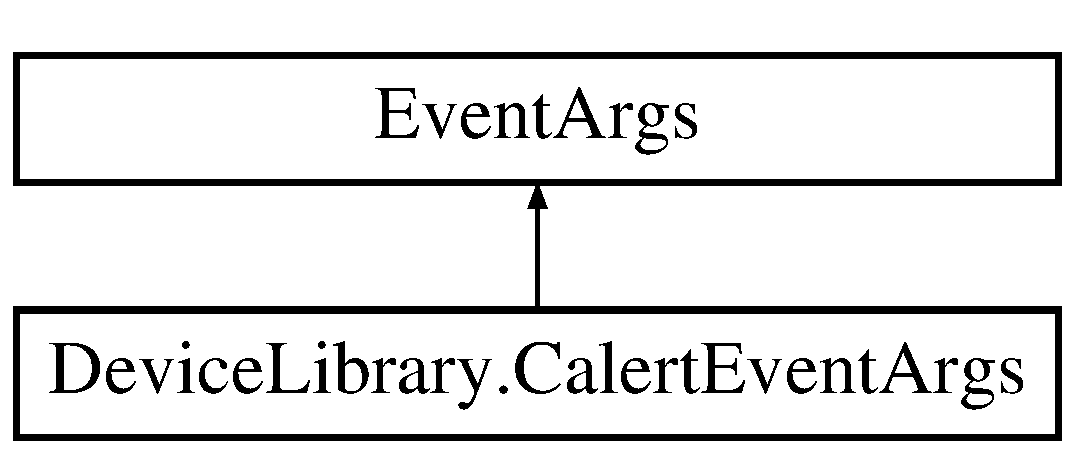
\includegraphics[height=2.000000cm]{class_device_library_1_1_calert_event_args}
\end{center}
\end{figure}
\subsection*{Public Attributes}
\begin{DoxyCompactItemize}
\item 
\mbox{\hyperlink{namespace_device_library_aecf5c8419c6482aed0b21decb1663754}{Reason}} \mbox{\hyperlink{class_device_library_1_1_calert_event_args_aefae78e9a96d2a95656c21c6e27fe2e6}{reason}}
\begin{DoxyCompactList}\small\item\em Cause de l\textquotesingle{}événement. \end{DoxyCompactList}\item 
object \mbox{\hyperlink{class_device_library_1_1_calert_event_args_a8af6a2546770e991696afd97029e57ff}{donnee}}
\begin{DoxyCompactList}\small\item\em Objet contenant les infomations concernant l\textquotesingle{}événement. \end{DoxyCompactList}\end{DoxyCompactItemize}


\subsection{Detailed Description}
Class d\textquotesingle{}évenement 



\subsection{Member Data Documentation}
\mbox{\Hypertarget{class_device_library_1_1_calert_event_args_a8af6a2546770e991696afd97029e57ff}\label{class_device_library_1_1_calert_event_args_a8af6a2546770e991696afd97029e57ff}} 
\index{Device\+Library\+::\+Calert\+Event\+Args@{Device\+Library\+::\+Calert\+Event\+Args}!donnee@{donnee}}
\index{donnee@{donnee}!Device\+Library\+::\+Calert\+Event\+Args@{Device\+Library\+::\+Calert\+Event\+Args}}
\subsubsection{\texorpdfstring{donnee}{donnee}}
{\footnotesize\ttfamily object Device\+Library.\+Calert\+Event\+Args.\+donnee}



Objet contenant les infomations concernant l\textquotesingle{}événement. 

\mbox{\Hypertarget{class_device_library_1_1_calert_event_args_aefae78e9a96d2a95656c21c6e27fe2e6}\label{class_device_library_1_1_calert_event_args_aefae78e9a96d2a95656c21c6e27fe2e6}} 
\index{Device\+Library\+::\+Calert\+Event\+Args@{Device\+Library\+::\+Calert\+Event\+Args}!reason@{reason}}
\index{reason@{reason}!Device\+Library\+::\+Calert\+Event\+Args@{Device\+Library\+::\+Calert\+Event\+Args}}
\subsubsection{\texorpdfstring{reason}{reason}}
{\footnotesize\ttfamily \mbox{\hyperlink{namespace_device_library_aecf5c8419c6482aed0b21decb1663754}{Reason}} Device\+Library.\+Calert\+Event\+Args.\+reason}



Cause de l\textquotesingle{}événement. 



The documentation for this class was generated from the following file\+:\begin{DoxyCompactItemize}
\item 
D\+:/\+Projets/\+A\+T\+M\+B/\+S\+O\+F\+T/\+Atmb\+Devices/\+Device\+Library/C\+Devices\+Manage.\+cs\end{DoxyCompactItemize}

\hypertarget{class_device_library_1_1_c_canal}{}\section{Device\+Library.\+C\+Canal Class Reference}
\label{class_device_library_1_1_c_canal}\index{Device\+Library.\+C\+Canal@{Device\+Library.\+C\+Canal}}


Class d\textquotesingle{}un canal d\textquotesingle{}un périphérique de paiement  


\subsection*{Classes}
\begin{DoxyCompactItemize}
\item 
class \mbox{\hyperlink{class_device_library_1_1_c_canal_1_1_c_coind_i_d}{C\+Coind\+ID}}
\begin{DoxyCompactList}\small\item\em Class gérant l\textquotesingle{}identification des pièces \end{DoxyCompactList}\item 
class \mbox{\hyperlink{class_device_library_1_1_c_canal_1_1_c_sorter}{C\+Sorter}}
\begin{DoxyCompactList}\small\item\em Class gérant les informations concernant un chemin de triage d\textquotesingle{}un canal \end{DoxyCompactList}\end{DoxyCompactItemize}
\subsection*{Public Member Functions}
\begin{DoxyCompactItemize}
\item 
\mbox{\hyperlink{class_device_library_1_1_c_canal_a31af2f08cfb27d40798116fdc0cfb372}{C\+Canal}} (byte number, \mbox{\hyperlink{class_device_library_1_1_c_coin_validator}{C\+Coin\+Validator}} owner)
\begin{DoxyCompactList}\small\item\em Constructeur \end{DoxyCompactList}\end{DoxyCompactItemize}
\subsection*{Public Attributes}
\begin{DoxyCompactItemize}
\item 
\mbox{\hyperlink{class_device_library_1_1_c_canal_1_1_c_coind_i_d}{C\+Coind\+ID}} \mbox{\hyperlink{class_device_library_1_1_c_canal_a5b9fc2885e84a372334c45007f8b5cf8}{coin\+Id}}
\begin{DoxyCompactList}\small\item\em Identification de la pièce reconnue dans le canal \end{DoxyCompactList}\item 
\mbox{\hyperlink{class_device_library_1_1_c_canal_1_1_c_sorter}{C\+Sorter}} \mbox{\hyperlink{class_device_library_1_1_c_canal_a15c9982533901ed86fcc0562a03d67df}{sorter}}
\begin{DoxyCompactList}\small\item\em Instance des chemins utilisés pour trier la pièce reconnue dans le canal \end{DoxyCompactList}\item 
byte \mbox{\hyperlink{class_device_library_1_1_c_canal_a5cb0d553ef6f6edc5a7268b1a427767b}{Number}}
\begin{DoxyCompactList}\small\item\em Numéro du canal \end{DoxyCompactList}\end{DoxyCompactItemize}
\subsection*{Properties}
\begin{DoxyCompactItemize}
\item 
byte \mbox{\hyperlink{class_device_library_1_1_c_canal_a4b920e01736bd1a067401c6cc76e2e4e}{Hopper\+To\+Load}}\hspace{0.3cm}{\ttfamily  \mbox{[}get, set\mbox{]}}
\begin{DoxyCompactList}\small\item\em Hopper vers lequel sera dirigé la pièce reconnue \end{DoxyCompactList}\item 
long \mbox{\hyperlink{class_device_library_1_1_c_canal_a01b652a04377f5daeb275adbad9ae1c2}{Coin\+In}}\hspace{0.3cm}{\ttfamily  \mbox{[}get, set\mbox{]}}
\begin{DoxyCompactList}\small\item\em Nombre de pièces reconnues par le canal. \end{DoxyCompactList}\item 
long \mbox{\hyperlink{class_device_library_1_1_c_canal_ac80e273e29e18b3f2b598aaf9f04506f}{Montant\+In}}\hspace{0.3cm}{\ttfamily  \mbox{[}get, set\mbox{]}}
\begin{DoxyCompactList}\small\item\em Montant introduit dans le canal \end{DoxyCompactList}\end{DoxyCompactItemize}


\subsection{Detailed Description}
Class d\textquotesingle{}un canal d\textquotesingle{}un périphérique de paiement 



\subsection{Constructor \& Destructor Documentation}
\mbox{\Hypertarget{class_device_library_1_1_c_canal_a31af2f08cfb27d40798116fdc0cfb372}\label{class_device_library_1_1_c_canal_a31af2f08cfb27d40798116fdc0cfb372}} 
\index{Device\+Library\+::\+C\+Canal@{Device\+Library\+::\+C\+Canal}!C\+Canal@{C\+Canal}}
\index{C\+Canal@{C\+Canal}!Device\+Library\+::\+C\+Canal@{Device\+Library\+::\+C\+Canal}}
\subsubsection{\texorpdfstring{C\+Canal()}{CCanal()}}
{\footnotesize\ttfamily Device\+Library.\+C\+Canal.\+C\+Canal (\begin{DoxyParamCaption}\item[{byte}]{number,  }\item[{\mbox{\hyperlink{class_device_library_1_1_c_coin_validator}{C\+Coin\+Validator}}}]{owner }\end{DoxyParamCaption})\hspace{0.3cm}{\ttfamily [inline]}}



Constructeur 


\begin{DoxyParams}{Parameters}
{\em number} & Numéro du canal\\
\hline
{\em owner} & Nécessaire pour effectuer les commandes\\
\hline
\end{DoxyParams}


\subsection{Member Data Documentation}
\mbox{\Hypertarget{class_device_library_1_1_c_canal_a5b9fc2885e84a372334c45007f8b5cf8}\label{class_device_library_1_1_c_canal_a5b9fc2885e84a372334c45007f8b5cf8}} 
\index{Device\+Library\+::\+C\+Canal@{Device\+Library\+::\+C\+Canal}!coin\+Id@{coin\+Id}}
\index{coin\+Id@{coin\+Id}!Device\+Library\+::\+C\+Canal@{Device\+Library\+::\+C\+Canal}}
\subsubsection{\texorpdfstring{coin\+Id}{coinId}}
{\footnotesize\ttfamily \mbox{\hyperlink{class_device_library_1_1_c_canal_1_1_c_coind_i_d}{C\+Coind\+ID}} Device\+Library.\+C\+Canal.\+coin\+Id}



Identification de la pièce reconnue dans le canal 

\mbox{\Hypertarget{class_device_library_1_1_c_canal_a5cb0d553ef6f6edc5a7268b1a427767b}\label{class_device_library_1_1_c_canal_a5cb0d553ef6f6edc5a7268b1a427767b}} 
\index{Device\+Library\+::\+C\+Canal@{Device\+Library\+::\+C\+Canal}!Number@{Number}}
\index{Number@{Number}!Device\+Library\+::\+C\+Canal@{Device\+Library\+::\+C\+Canal}}
\subsubsection{\texorpdfstring{Number}{Number}}
{\footnotesize\ttfamily byte Device\+Library.\+C\+Canal.\+Number}



Numéro du canal 

\mbox{\Hypertarget{class_device_library_1_1_c_canal_a15c9982533901ed86fcc0562a03d67df}\label{class_device_library_1_1_c_canal_a15c9982533901ed86fcc0562a03d67df}} 
\index{Device\+Library\+::\+C\+Canal@{Device\+Library\+::\+C\+Canal}!sorter@{sorter}}
\index{sorter@{sorter}!Device\+Library\+::\+C\+Canal@{Device\+Library\+::\+C\+Canal}}
\subsubsection{\texorpdfstring{sorter}{sorter}}
{\footnotesize\ttfamily \mbox{\hyperlink{class_device_library_1_1_c_canal_1_1_c_sorter}{C\+Sorter}} Device\+Library.\+C\+Canal.\+sorter}



Instance des chemins utilisés pour trier la pièce reconnue dans le canal 



\subsection{Property Documentation}
\mbox{\Hypertarget{class_device_library_1_1_c_canal_a01b652a04377f5daeb275adbad9ae1c2}\label{class_device_library_1_1_c_canal_a01b652a04377f5daeb275adbad9ae1c2}} 
\index{Device\+Library\+::\+C\+Canal@{Device\+Library\+::\+C\+Canal}!Coin\+In@{Coin\+In}}
\index{Coin\+In@{Coin\+In}!Device\+Library\+::\+C\+Canal@{Device\+Library\+::\+C\+Canal}}
\subsubsection{\texorpdfstring{Coin\+In}{CoinIn}}
{\footnotesize\ttfamily long Device\+Library.\+C\+Canal.\+Coin\+In\hspace{0.3cm}{\ttfamily [get]}, {\ttfamily [set]}}



Nombre de pièces reconnues par le canal. 

\mbox{\Hypertarget{class_device_library_1_1_c_canal_a4b920e01736bd1a067401c6cc76e2e4e}\label{class_device_library_1_1_c_canal_a4b920e01736bd1a067401c6cc76e2e4e}} 
\index{Device\+Library\+::\+C\+Canal@{Device\+Library\+::\+C\+Canal}!Hopper\+To\+Load@{Hopper\+To\+Load}}
\index{Hopper\+To\+Load@{Hopper\+To\+Load}!Device\+Library\+::\+C\+Canal@{Device\+Library\+::\+C\+Canal}}
\subsubsection{\texorpdfstring{Hopper\+To\+Load}{HopperToLoad}}
{\footnotesize\ttfamily byte Device\+Library.\+C\+Canal.\+Hopper\+To\+Load\hspace{0.3cm}{\ttfamily [get]}, {\ttfamily [set]}}



Hopper vers lequel sera dirigé la pièce reconnue 

\mbox{\Hypertarget{class_device_library_1_1_c_canal_ac80e273e29e18b3f2b598aaf9f04506f}\label{class_device_library_1_1_c_canal_ac80e273e29e18b3f2b598aaf9f04506f}} 
\index{Device\+Library\+::\+C\+Canal@{Device\+Library\+::\+C\+Canal}!Montant\+In@{Montant\+In}}
\index{Montant\+In@{Montant\+In}!Device\+Library\+::\+C\+Canal@{Device\+Library\+::\+C\+Canal}}
\subsubsection{\texorpdfstring{Montant\+In}{MontantIn}}
{\footnotesize\ttfamily long Device\+Library.\+C\+Canal.\+Montant\+In\hspace{0.3cm}{\ttfamily [get]}, {\ttfamily [set]}}



Montant introduit dans le canal 



The documentation for this class was generated from the following file\+:\begin{DoxyCompactItemize}
\item 
D\+:/\+Projets/\+A\+T\+M\+B/\+S\+O\+F\+T/\+Atmb\+Devices/\+Device\+Library/C\+Canal.\+cs\end{DoxyCompactItemize}

\hypertarget{class_device_library_1_1_ccash_reader}{}\section{Device\+Library.\+Ccash\+Reader Class Reference}
\label{class_device_library_1_1_ccash_reader}\index{Device\+Library.\+Ccash\+Reader@{Device\+Library.\+Ccash\+Reader}}


Class abstraite utilisé par les moyens de paiement.  


Inheritance diagram for Device\+Library.\+Ccash\+Reader\+:\begin{figure}[H]
\begin{center}
\leavevmode
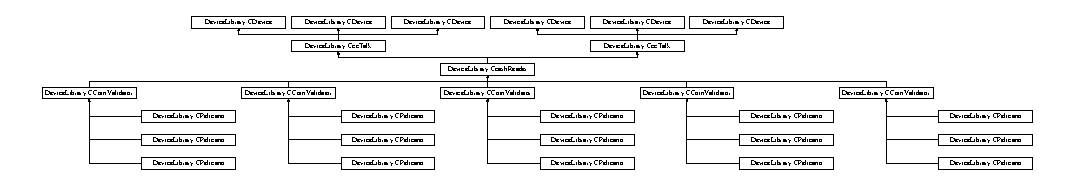
\includegraphics[height=2.052356cm]{class_device_library_1_1_ccash_reader}
\end{center}
\end{figure}
\subsection*{Public Member Functions}
\begin{DoxyCompactItemize}
\item 
void \mbox{\hyperlink{class_device_library_1_1_ccash_reader_aec351cc4aeaf3fd814808de16bbc97f7}{Master\+Enable}} ()
\begin{DoxyCompactList}\small\item\em Activation globale du moyen de paiement \end{DoxyCompactList}\item 
void \mbox{\hyperlink{class_device_library_1_1_ccash_reader_acd4d9cf6f8ee0299f5521b6ff6fabc57}{Master\+Disable}} ()
\begin{DoxyCompactList}\small\item\em Desactive globalement le moyen de paiement \end{DoxyCompactList}\item 
void \mbox{\hyperlink{class_device_library_1_1_ccash_reader_ae336729983d06e5d15b9935a5d380417}{Set\+Inhibit\+Status}} (byte\mbox{[}$\,$\mbox{]} mask)
\begin{DoxyCompactList}\small\item\em Active ou desactive les canaux du monnayeur \end{DoxyCompactList}\item 
void \mbox{\hyperlink{class_device_library_1_1_ccash_reader_a22cc54c81546b8e13ca08d5981c791cf}{Get\+Inhibit\+Mask}} (byte\mbox{[}$\,$\mbox{]} mask)
\begin{DoxyCompactList}\small\item\em Retourne le mask d\textquotesingle{}inhibition des canaux \end{DoxyCompactList}\item 
abstract void \mbox{\hyperlink{class_device_library_1_1_ccash_reader_ab2ea8031995213b54aa9801f86f15315}{Task\+Check\+Event\+CV}} ()
\begin{DoxyCompactList}\small\item\em Tâche vérifiant les activitées du monnayeur \end{DoxyCompactList}\end{DoxyCompactItemize}
\subsection*{Protected Types}
\begin{DoxyCompactItemize}
\item 
enum \mbox{\hyperlink{class_device_library_1_1_ccash_reader_a789dcffa38ad9d646e32c448632ceaff}{Inhibit\+Status}} \{ \mbox{\hyperlink{class_device_library_1_1_ccash_reader_a789dcffa38ad9d646e32c448632ceaffa055c1a591abb0e8cd86dc969727bcc0b}{Inhibit\+Status.\+D\+I\+S\+A\+B\+L\+ED}} = 0, 
\mbox{\hyperlink{class_device_library_1_1_ccash_reader_a789dcffa38ad9d646e32c448632ceaffac8cf6eea8f096ed51160b484d97c5bbd}{Inhibit\+Status.\+E\+N\+A\+B\+L\+ED}} = 1
 \}
\begin{DoxyCompactList}\small\item\em Enumération des ihnibitions. \end{DoxyCompactList}\item 
enum \mbox{\hyperlink{class_device_library_1_1_ccash_reader_af4bdeeddb7c89dd2b54f86978f5e9866}{Header}} \+: byte \{ \newline
\mbox{\hyperlink{class_device_library_1_1_ccash_reader_af4bdeeddb7c89dd2b54f86978f5e9866ae528792c78a8f0df73cb539242c9db57}{Header.\+R\+E\+Q\+U\+E\+S\+T\+P\+O\+L\+L\+I\+N\+G\+P\+R\+I\+O\+R\+I\+TY}} = 249, 
\mbox{\hyperlink{class_device_library_1_1_ccash_reader_af4bdeeddb7c89dd2b54f86978f5e9866ae268218a830fbe959f8a433163e8187a}{Header.\+P\+E\+R\+F\+O\+R\+M\+S\+E\+L\+F\+T\+E\+ST}} = 232, 
\mbox{\hyperlink{class_device_library_1_1_ccash_reader_af4bdeeddb7c89dd2b54f86978f5e9866a57fa2152134db32c8ccf2c03fd965489}{Header.\+M\+O\+D\+I\+F\+Y\+I\+N\+H\+I\+B\+I\+T\+S\+T\+A\+T\+US}} = 231, 
\mbox{\hyperlink{class_device_library_1_1_ccash_reader_af4bdeeddb7c89dd2b54f86978f5e9866a86d5eb66e4f787072c88909f8de0ee99}{Header.\+R\+E\+Q\+U\+E\+S\+T\+I\+N\+H\+I\+B\+I\+T\+S\+T\+A\+T\+US}} = 230, 
\newline
\mbox{\hyperlink{class_device_library_1_1_ccash_reader_af4bdeeddb7c89dd2b54f86978f5e9866aa932deef49f85794660b6e9b0fd2f426}{Header.\+M\+O\+D\+I\+F\+Y\+M\+A\+S\+T\+E\+R\+I\+N\+H\+I\+B\+I\+T\+S\+T\+A\+T\+US}} = 228, 
\mbox{\hyperlink{class_device_library_1_1_ccash_reader_af4bdeeddb7c89dd2b54f86978f5e9866a9feb77035916af7a4a90c7e62047cee0}{Header.\+R\+E\+Q\+U\+E\+S\+T\+M\+A\+S\+T\+E\+R\+I\+N\+H\+I\+B\+I\+T\+S\+T\+A\+T\+US}} = 227
 \}
\begin{DoxyCompactList}\small\item\em Enumeration des headers concernant les moyens de peiement \end{DoxyCompactList}\end{DoxyCompactItemize}
\subsection*{Properties}
\begin{DoxyCompactItemize}
\item 
byte \mbox{[}$\,$\mbox{]} \mbox{\hyperlink{class_device_library_1_1_ccash_reader_a566a8b5bf9b1f377c5439f06a6d58178}{Inhibit\+Mask}}\hspace{0.3cm}{\ttfamily  \mbox{[}get, set\mbox{]}}
\begin{DoxyCompactList}\small\item\em Masque d\textquotesingle{}ihnibition (2 octets pour 16 canaux) \end{DoxyCompactList}\item 
int \mbox{\hyperlink{class_device_library_1_1_ccash_reader_a5378d4373a02c46261c7f611af60a89c}{Polling\+Delay}}\hspace{0.3cm}{\ttfamily  \mbox{[}get, set\mbox{]}}
\begin{DoxyCompactList}\small\item\em Délai entre 2 interrogation du coin validator. \end{DoxyCompactList}\item 
\mbox{\hyperlink{class_device_library_1_1_ccash_reader_a789dcffa38ad9d646e32c448632ceaff}{Inhibit\+Status}} \mbox{\hyperlink{class_device_library_1_1_ccash_reader_ad6efa8899adedbb445d7f7cb4af0c159}{Master\+Inhibit\+Status}}\hspace{0.3cm}{\ttfamily  \mbox{[}get\mbox{]}}
\begin{DoxyCompactList}\small\item\em Renvoi l\textquotesingle{}activation du monnayeur \end{DoxyCompactList}\item 
int \mbox{\hyperlink{class_device_library_1_1_ccash_reader_a1768cb2711e0f8d8fd45d9d28aeb1cf6}{Polling\+Priority}}\hspace{0.3cm}{\ttfamily  \mbox{[}get\mbox{]}}
\begin{DoxyCompactList}\small\item\em Renvoi le délai maximum du polling du périphérique. \end{DoxyCompactList}\item 
\mbox{\hyperlink{group___erreur_ga179570d2d8f6f95d52ccafb98d20c790}{Self\+Test\+Result}} \mbox{\hyperlink{class_device_library_1_1_ccash_reader_a40798e7b17783bffe4d59b67ef57a430}{Self\+Test}}\hspace{0.3cm}{\ttfamily  \mbox{[}get\mbox{]}}
\begin{DoxyCompactList}\small\item\em Effectue un test interne et renvoie le résultat. \end{DoxyCompactList}\end{DoxyCompactItemize}
\subsection*{Additional Inherited Members}


\subsection{Detailed Description}
Class abstraite utilisé par les moyens de paiement. 



\subsection{Member Enumeration Documentation}
\mbox{\Hypertarget{class_device_library_1_1_ccash_reader_af4bdeeddb7c89dd2b54f86978f5e9866}\label{class_device_library_1_1_ccash_reader_af4bdeeddb7c89dd2b54f86978f5e9866}} 
\index{Device\+Library\+::\+Ccash\+Reader@{Device\+Library\+::\+Ccash\+Reader}!Header@{Header}}
\index{Header@{Header}!Device\+Library\+::\+Ccash\+Reader@{Device\+Library\+::\+Ccash\+Reader}}
\subsubsection{\texorpdfstring{Header}{Header}}
{\footnotesize\ttfamily enum \mbox{\hyperlink{class_device_library_1_1_ccash_reader_af4bdeeddb7c89dd2b54f86978f5e9866}{Device\+Library.\+Ccash\+Reader.\+Header}} \+: byte\hspace{0.3cm}{\ttfamily [strong]}, {\ttfamily [protected]}}



Enumeration des headers concernant les moyens de peiement 

\begin{DoxyEnumFields}{Enumerator}
\raisebox{\heightof{T}}[0pt][0pt]{\index{R\+E\+Q\+U\+E\+S\+T\+P\+O\+L\+L\+I\+N\+G\+P\+R\+I\+O\+R\+I\+TY@{R\+E\+Q\+U\+E\+S\+T\+P\+O\+L\+L\+I\+N\+G\+P\+R\+I\+O\+R\+I\+TY}!Device\+Library\+::\+Ccash\+Reader@{Device\+Library\+::\+Ccash\+Reader}}\index{Device\+Library\+::\+Ccash\+Reader@{Device\+Library\+::\+Ccash\+Reader}!R\+E\+Q\+U\+E\+S\+T\+P\+O\+L\+L\+I\+N\+G\+P\+R\+I\+O\+R\+I\+TY@{R\+E\+Q\+U\+E\+S\+T\+P\+O\+L\+L\+I\+N\+G\+P\+R\+I\+O\+R\+I\+TY}}}\mbox{\Hypertarget{class_device_library_1_1_ccash_reader_af4bdeeddb7c89dd2b54f86978f5e9866ae528792c78a8f0df73cb539242c9db57}\label{class_device_library_1_1_ccash_reader_af4bdeeddb7c89dd2b54f86978f5e9866ae528792c78a8f0df73cb539242c9db57}} 
R\+E\+Q\+U\+E\+S\+T\+P\+O\+L\+L\+I\+N\+G\+P\+R\+I\+O\+R\+I\+TY&Délai recommandé pour vérifier le buffer de crédits et de code d\textquotesingle{}erreur Au dela de ce délai le périphérique devrait être désactivé\\
\hline

\raisebox{\heightof{T}}[0pt][0pt]{\index{P\+E\+R\+F\+O\+R\+M\+S\+E\+L\+F\+T\+E\+ST@{P\+E\+R\+F\+O\+R\+M\+S\+E\+L\+F\+T\+E\+ST}!Device\+Library\+::\+Ccash\+Reader@{Device\+Library\+::\+Ccash\+Reader}}\index{Device\+Library\+::\+Ccash\+Reader@{Device\+Library\+::\+Ccash\+Reader}!P\+E\+R\+F\+O\+R\+M\+S\+E\+L\+F\+T\+E\+ST@{P\+E\+R\+F\+O\+R\+M\+S\+E\+L\+F\+T\+E\+ST}}}\mbox{\Hypertarget{class_device_library_1_1_ccash_reader_af4bdeeddb7c89dd2b54f86978f5e9866ae268218a830fbe959f8a433163e8187a}\label{class_device_library_1_1_ccash_reader_af4bdeeddb7c89dd2b54f86978f5e9866ae268218a830fbe959f8a433163e8187a}} 
P\+E\+R\+F\+O\+R\+M\+S\+E\+L\+F\+T\+E\+ST&Cette commande effectue un test interne. \\
\hline

\raisebox{\heightof{T}}[0pt][0pt]{\index{M\+O\+D\+I\+F\+Y\+I\+N\+H\+I\+B\+I\+T\+S\+T\+A\+T\+US@{M\+O\+D\+I\+F\+Y\+I\+N\+H\+I\+B\+I\+T\+S\+T\+A\+T\+US}!Device\+Library\+::\+Ccash\+Reader@{Device\+Library\+::\+Ccash\+Reader}}\index{Device\+Library\+::\+Ccash\+Reader@{Device\+Library\+::\+Ccash\+Reader}!M\+O\+D\+I\+F\+Y\+I\+N\+H\+I\+B\+I\+T\+S\+T\+A\+T\+US@{M\+O\+D\+I\+F\+Y\+I\+N\+H\+I\+B\+I\+T\+S\+T\+A\+T\+US}}}\mbox{\Hypertarget{class_device_library_1_1_ccash_reader_af4bdeeddb7c89dd2b54f86978f5e9866a57fa2152134db32c8ccf2c03fd965489}\label{class_device_library_1_1_ccash_reader_af4bdeeddb7c89dd2b54f86978f5e9866a57fa2152134db32c8ccf2c03fd965489}} 
M\+O\+D\+I\+F\+Y\+I\+N\+H\+I\+B\+I\+T\+S\+T\+A\+T\+US&Cette commande envoie un masque d\textquotesingle{}inhibition. Chaque bit correspondant à un canal 0 = desactivé, 1 = activé\\
\hline

\raisebox{\heightof{T}}[0pt][0pt]{\index{R\+E\+Q\+U\+E\+S\+T\+I\+N\+H\+I\+B\+I\+T\+S\+T\+A\+T\+US@{R\+E\+Q\+U\+E\+S\+T\+I\+N\+H\+I\+B\+I\+T\+S\+T\+A\+T\+US}!Device\+Library\+::\+Ccash\+Reader@{Device\+Library\+::\+Ccash\+Reader}}\index{Device\+Library\+::\+Ccash\+Reader@{Device\+Library\+::\+Ccash\+Reader}!R\+E\+Q\+U\+E\+S\+T\+I\+N\+H\+I\+B\+I\+T\+S\+T\+A\+T\+US@{R\+E\+Q\+U\+E\+S\+T\+I\+N\+H\+I\+B\+I\+T\+S\+T\+A\+T\+US}}}\mbox{\Hypertarget{class_device_library_1_1_ccash_reader_af4bdeeddb7c89dd2b54f86978f5e9866a86d5eb66e4f787072c88909f8de0ee99}\label{class_device_library_1_1_ccash_reader_af4bdeeddb7c89dd2b54f86978f5e9866a86d5eb66e4f787072c88909f8de0ee99}} 
R\+E\+Q\+U\+E\+S\+T\+I\+N\+H\+I\+B\+I\+T\+S\+T\+A\+T\+US&Demande le masque d\textquotesingle{}inhibition voir M\+O\+D\+I\+F\+Y\+I\+N\+H\+I\+B\+I\+T\+S\+T\+A\+T\+US \\
\hline

\raisebox{\heightof{T}}[0pt][0pt]{\index{M\+O\+D\+I\+F\+Y\+M\+A\+S\+T\+E\+R\+I\+N\+H\+I\+B\+I\+T\+S\+T\+A\+T\+US@{M\+O\+D\+I\+F\+Y\+M\+A\+S\+T\+E\+R\+I\+N\+H\+I\+B\+I\+T\+S\+T\+A\+T\+US}!Device\+Library\+::\+Ccash\+Reader@{Device\+Library\+::\+Ccash\+Reader}}\index{Device\+Library\+::\+Ccash\+Reader@{Device\+Library\+::\+Ccash\+Reader}!M\+O\+D\+I\+F\+Y\+M\+A\+S\+T\+E\+R\+I\+N\+H\+I\+B\+I\+T\+S\+T\+A\+T\+US@{M\+O\+D\+I\+F\+Y\+M\+A\+S\+T\+E\+R\+I\+N\+H\+I\+B\+I\+T\+S\+T\+A\+T\+US}}}\mbox{\Hypertarget{class_device_library_1_1_ccash_reader_af4bdeeddb7c89dd2b54f86978f5e9866aa932deef49f85794660b6e9b0fd2f426}\label{class_device_library_1_1_ccash_reader_af4bdeeddb7c89dd2b54f86978f5e9866aa932deef49f85794660b6e9b0fd2f426}} 
M\+O\+D\+I\+F\+Y\+M\+A\+S\+T\+E\+R\+I\+N\+H\+I\+B\+I\+T\+S\+T\+A\+T\+US&Cette commande envoie un masque d\textquotesingle{}inhibition géneral au périphérique. Seul le bit de poid faible est pris en considération\\
\hline

\raisebox{\heightof{T}}[0pt][0pt]{\index{R\+E\+Q\+U\+E\+S\+T\+M\+A\+S\+T\+E\+R\+I\+N\+H\+I\+B\+I\+T\+S\+T\+A\+T\+US@{R\+E\+Q\+U\+E\+S\+T\+M\+A\+S\+T\+E\+R\+I\+N\+H\+I\+B\+I\+T\+S\+T\+A\+T\+US}!Device\+Library\+::\+Ccash\+Reader@{Device\+Library\+::\+Ccash\+Reader}}\index{Device\+Library\+::\+Ccash\+Reader@{Device\+Library\+::\+Ccash\+Reader}!R\+E\+Q\+U\+E\+S\+T\+M\+A\+S\+T\+E\+R\+I\+N\+H\+I\+B\+I\+T\+S\+T\+A\+T\+US@{R\+E\+Q\+U\+E\+S\+T\+M\+A\+S\+T\+E\+R\+I\+N\+H\+I\+B\+I\+T\+S\+T\+A\+T\+US}}}\mbox{\Hypertarget{class_device_library_1_1_ccash_reader_af4bdeeddb7c89dd2b54f86978f5e9866a9feb77035916af7a4a90c7e62047cee0}\label{class_device_library_1_1_ccash_reader_af4bdeeddb7c89dd2b54f86978f5e9866a9feb77035916af7a4a90c7e62047cee0}} 
R\+E\+Q\+U\+E\+S\+T\+M\+A\+S\+T\+E\+R\+I\+N\+H\+I\+B\+I\+T\+S\+T\+A\+T\+US&Cette commande demande le masque d\textquotesingle{}inhibition géneral du périphérique ~\newline
 voir M\+O\+D\+I\+F\+Y\+M\+A\+S\+T\+E\+R\+I\+N\+H\+I\+B\+I\+T\+S\+T\+A\+T\+US\\
\hline

\end{DoxyEnumFields}
\mbox{\Hypertarget{class_device_library_1_1_ccash_reader_a789dcffa38ad9d646e32c448632ceaff}\label{class_device_library_1_1_ccash_reader_a789dcffa38ad9d646e32c448632ceaff}} 
\index{Device\+Library\+::\+Ccash\+Reader@{Device\+Library\+::\+Ccash\+Reader}!Inhibit\+Status@{Inhibit\+Status}}
\index{Inhibit\+Status@{Inhibit\+Status}!Device\+Library\+::\+Ccash\+Reader@{Device\+Library\+::\+Ccash\+Reader}}
\subsubsection{\texorpdfstring{Inhibit\+Status}{InhibitStatus}}
{\footnotesize\ttfamily enum \mbox{\hyperlink{class_device_library_1_1_ccash_reader_a789dcffa38ad9d646e32c448632ceaff}{Device\+Library.\+Ccash\+Reader.\+Inhibit\+Status}}\hspace{0.3cm}{\ttfamily [strong]}, {\ttfamily [protected]}}



Enumération des ihnibitions. 

\begin{DoxyEnumFields}{Enumerator}
\raisebox{\heightof{T}}[0pt][0pt]{\index{D\+I\+S\+A\+B\+L\+ED@{D\+I\+S\+A\+B\+L\+ED}!Device\+Library\+::\+Ccash\+Reader@{Device\+Library\+::\+Ccash\+Reader}}\index{Device\+Library\+::\+Ccash\+Reader@{Device\+Library\+::\+Ccash\+Reader}!D\+I\+S\+A\+B\+L\+ED@{D\+I\+S\+A\+B\+L\+ED}}}\mbox{\Hypertarget{class_device_library_1_1_ccash_reader_a789dcffa38ad9d646e32c448632ceaffa055c1a591abb0e8cd86dc969727bcc0b}\label{class_device_library_1_1_ccash_reader_a789dcffa38ad9d646e32c448632ceaffa055c1a591abb0e8cd86dc969727bcc0b}} 
D\+I\+S\+A\+B\+L\+ED&Périphérique désactivé \\
\hline

\raisebox{\heightof{T}}[0pt][0pt]{\index{E\+N\+A\+B\+L\+ED@{E\+N\+A\+B\+L\+ED}!Device\+Library\+::\+Ccash\+Reader@{Device\+Library\+::\+Ccash\+Reader}}\index{Device\+Library\+::\+Ccash\+Reader@{Device\+Library\+::\+Ccash\+Reader}!E\+N\+A\+B\+L\+ED@{E\+N\+A\+B\+L\+ED}}}\mbox{\Hypertarget{class_device_library_1_1_ccash_reader_a789dcffa38ad9d646e32c448632ceaffac8cf6eea8f096ed51160b484d97c5bbd}\label{class_device_library_1_1_ccash_reader_a789dcffa38ad9d646e32c448632ceaffac8cf6eea8f096ed51160b484d97c5bbd}} 
E\+N\+A\+B\+L\+ED&Périphérique activé \\
\hline

\end{DoxyEnumFields}


\subsection{Member Function Documentation}
\mbox{\Hypertarget{class_device_library_1_1_ccash_reader_a22cc54c81546b8e13ca08d5981c791cf}\label{class_device_library_1_1_ccash_reader_a22cc54c81546b8e13ca08d5981c791cf}} 
\index{Device\+Library\+::\+Ccash\+Reader@{Device\+Library\+::\+Ccash\+Reader}!Get\+Inhibit\+Mask@{Get\+Inhibit\+Mask}}
\index{Get\+Inhibit\+Mask@{Get\+Inhibit\+Mask}!Device\+Library\+::\+Ccash\+Reader@{Device\+Library\+::\+Ccash\+Reader}}
\subsubsection{\texorpdfstring{Get\+Inhibit\+Mask()}{GetInhibitMask()}}
{\footnotesize\ttfamily void Device\+Library.\+Ccash\+Reader.\+Get\+Inhibit\+Mask (\begin{DoxyParamCaption}\item[{byte \mbox{[}$\,$\mbox{]}}]{mask }\end{DoxyParamCaption})\hspace{0.3cm}{\ttfamily [inline]}}



Retourne le mask d\textquotesingle{}inhibition des canaux 


\begin{DoxyParams}{Parameters}
{\em mask} & Buffer contenant les masks d\textquotesingle{}inhibitions\\
\hline
\end{DoxyParams}
\mbox{\Hypertarget{class_device_library_1_1_ccash_reader_acd4d9cf6f8ee0299f5521b6ff6fabc57}\label{class_device_library_1_1_ccash_reader_acd4d9cf6f8ee0299f5521b6ff6fabc57}} 
\index{Device\+Library\+::\+Ccash\+Reader@{Device\+Library\+::\+Ccash\+Reader}!Master\+Disable@{Master\+Disable}}
\index{Master\+Disable@{Master\+Disable}!Device\+Library\+::\+Ccash\+Reader@{Device\+Library\+::\+Ccash\+Reader}}
\subsubsection{\texorpdfstring{Master\+Disable()}{MasterDisable()}}
{\footnotesize\ttfamily void Device\+Library.\+Ccash\+Reader.\+Master\+Disable (\begin{DoxyParamCaption}{ }\end{DoxyParamCaption})\hspace{0.3cm}{\ttfamily [inline]}}



Desactive globalement le moyen de paiement 

\mbox{\Hypertarget{class_device_library_1_1_ccash_reader_aec351cc4aeaf3fd814808de16bbc97f7}\label{class_device_library_1_1_ccash_reader_aec351cc4aeaf3fd814808de16bbc97f7}} 
\index{Device\+Library\+::\+Ccash\+Reader@{Device\+Library\+::\+Ccash\+Reader}!Master\+Enable@{Master\+Enable}}
\index{Master\+Enable@{Master\+Enable}!Device\+Library\+::\+Ccash\+Reader@{Device\+Library\+::\+Ccash\+Reader}}
\subsubsection{\texorpdfstring{Master\+Enable()}{MasterEnable()}}
{\footnotesize\ttfamily void Device\+Library.\+Ccash\+Reader.\+Master\+Enable (\begin{DoxyParamCaption}{ }\end{DoxyParamCaption})\hspace{0.3cm}{\ttfamily [inline]}}



Activation globale du moyen de paiement 

\mbox{\Hypertarget{class_device_library_1_1_ccash_reader_ae336729983d06e5d15b9935a5d380417}\label{class_device_library_1_1_ccash_reader_ae336729983d06e5d15b9935a5d380417}} 
\index{Device\+Library\+::\+Ccash\+Reader@{Device\+Library\+::\+Ccash\+Reader}!Set\+Inhibit\+Status@{Set\+Inhibit\+Status}}
\index{Set\+Inhibit\+Status@{Set\+Inhibit\+Status}!Device\+Library\+::\+Ccash\+Reader@{Device\+Library\+::\+Ccash\+Reader}}
\subsubsection{\texorpdfstring{Set\+Inhibit\+Status()}{SetInhibitStatus()}}
{\footnotesize\ttfamily void Device\+Library.\+Ccash\+Reader.\+Set\+Inhibit\+Status (\begin{DoxyParamCaption}\item[{byte \mbox{[}$\,$\mbox{]}}]{mask }\end{DoxyParamCaption})\hspace{0.3cm}{\ttfamily [inline]}}



Active ou desactive les canaux du monnayeur 


\begin{DoxyParams}{Parameters}
{\em mask} & masque d\textquotesingle{}inhibiton\\
\hline
\end{DoxyParams}


Header 231\mbox{\Hypertarget{class_device_library_1_1_ccash_reader_ab2ea8031995213b54aa9801f86f15315}\label{class_device_library_1_1_ccash_reader_ab2ea8031995213b54aa9801f86f15315}} 
\index{Device\+Library\+::\+Ccash\+Reader@{Device\+Library\+::\+Ccash\+Reader}!Task\+Check\+Event\+CV@{Task\+Check\+Event\+CV}}
\index{Task\+Check\+Event\+CV@{Task\+Check\+Event\+CV}!Device\+Library\+::\+Ccash\+Reader@{Device\+Library\+::\+Ccash\+Reader}}
\subsubsection{\texorpdfstring{Task\+Check\+Event\+C\+V()}{TaskCheckEventCV()}}
{\footnotesize\ttfamily abstract void Device\+Library.\+Ccash\+Reader.\+Task\+Check\+Event\+CV (\begin{DoxyParamCaption}{ }\end{DoxyParamCaption})\hspace{0.3cm}{\ttfamily [pure virtual]}}



Tâche vérifiant les activitées du monnayeur 



Implemented in \mbox{\hyperlink{class_device_library_1_1_c_coin_validator_a0e406f9e175eb8d295fe7406e6a948af}{Device\+Library.\+C\+Coin\+Validator}}, and \mbox{\hyperlink{class_device_library_1_1_c_pelicano_a38a0d7a675ff22773f5eb153fab9275a}{Device\+Library.\+C\+Pelicano}}.



\subsection{Property Documentation}
\mbox{\Hypertarget{class_device_library_1_1_ccash_reader_a566a8b5bf9b1f377c5439f06a6d58178}\label{class_device_library_1_1_ccash_reader_a566a8b5bf9b1f377c5439f06a6d58178}} 
\index{Device\+Library\+::\+Ccash\+Reader@{Device\+Library\+::\+Ccash\+Reader}!Inhibit\+Mask@{Inhibit\+Mask}}
\index{Inhibit\+Mask@{Inhibit\+Mask}!Device\+Library\+::\+Ccash\+Reader@{Device\+Library\+::\+Ccash\+Reader}}
\subsubsection{\texorpdfstring{Inhibit\+Mask}{InhibitMask}}
{\footnotesize\ttfamily byte \mbox{[}$\,$\mbox{]} Device\+Library.\+Ccash\+Reader.\+Inhibit\+Mask\hspace{0.3cm}{\ttfamily [get]}, {\ttfamily [set]}, {\ttfamily [protected]}}



Masque d\textquotesingle{}ihnibition (2 octets pour 16 canaux) 

\mbox{\Hypertarget{class_device_library_1_1_ccash_reader_ad6efa8899adedbb445d7f7cb4af0c159}\label{class_device_library_1_1_ccash_reader_ad6efa8899adedbb445d7f7cb4af0c159}} 
\index{Device\+Library\+::\+Ccash\+Reader@{Device\+Library\+::\+Ccash\+Reader}!Master\+Inhibit\+Status@{Master\+Inhibit\+Status}}
\index{Master\+Inhibit\+Status@{Master\+Inhibit\+Status}!Device\+Library\+::\+Ccash\+Reader@{Device\+Library\+::\+Ccash\+Reader}}
\subsubsection{\texorpdfstring{Master\+Inhibit\+Status}{MasterInhibitStatus}}
{\footnotesize\ttfamily \mbox{\hyperlink{class_device_library_1_1_ccash_reader_a789dcffa38ad9d646e32c448632ceaff}{Inhibit\+Status}} Device\+Library.\+Ccash\+Reader.\+Master\+Inhibit\+Status\hspace{0.3cm}{\ttfamily [get]}, {\ttfamily [protected]}}



Renvoi l\textquotesingle{}activation du monnayeur 

\begin{DoxyReturn}{Returns}
E\+N\+A\+B\+L\+ED si le monnayeur est activé D\+I\+S\+A\+B\+L\+ED si le monnayeur est désactivé 
\end{DoxyReturn}


Header 227\mbox{\Hypertarget{class_device_library_1_1_ccash_reader_a5378d4373a02c46261c7f611af60a89c}\label{class_device_library_1_1_ccash_reader_a5378d4373a02c46261c7f611af60a89c}} 
\index{Device\+Library\+::\+Ccash\+Reader@{Device\+Library\+::\+Ccash\+Reader}!Polling\+Delay@{Polling\+Delay}}
\index{Polling\+Delay@{Polling\+Delay}!Device\+Library\+::\+Ccash\+Reader@{Device\+Library\+::\+Ccash\+Reader}}
\subsubsection{\texorpdfstring{Polling\+Delay}{PollingDelay}}
{\footnotesize\ttfamily int Device\+Library.\+Ccash\+Reader.\+Polling\+Delay\hspace{0.3cm}{\ttfamily [get]}, {\ttfamily [set]}, {\ttfamily [protected]}}



Délai entre 2 interrogation du coin validator. 

\mbox{\Hypertarget{class_device_library_1_1_ccash_reader_a1768cb2711e0f8d8fd45d9d28aeb1cf6}\label{class_device_library_1_1_ccash_reader_a1768cb2711e0f8d8fd45d9d28aeb1cf6}} 
\index{Device\+Library\+::\+Ccash\+Reader@{Device\+Library\+::\+Ccash\+Reader}!Polling\+Priority@{Polling\+Priority}}
\index{Polling\+Priority@{Polling\+Priority}!Device\+Library\+::\+Ccash\+Reader@{Device\+Library\+::\+Ccash\+Reader}}
\subsubsection{\texorpdfstring{Polling\+Priority}{PollingPriority}}
{\footnotesize\ttfamily int Device\+Library.\+Ccash\+Reader.\+Polling\+Priority\hspace{0.3cm}{\ttfamily [get]}, {\ttfamily [protected]}}



Renvoi le délai maximum du polling du périphérique. 

Header 249

\begin{DoxyReturn}{Returns}
Délai du polling ou 0 en cas d\textquotesingle{}échec de traitement
\end{DoxyReturn}
\mbox{\Hypertarget{class_device_library_1_1_ccash_reader_a40798e7b17783bffe4d59b67ef57a430}\label{class_device_library_1_1_ccash_reader_a40798e7b17783bffe4d59b67ef57a430}} 
\index{Device\+Library\+::\+Ccash\+Reader@{Device\+Library\+::\+Ccash\+Reader}!Self\+Test@{Self\+Test}}
\index{Self\+Test@{Self\+Test}!Device\+Library\+::\+Ccash\+Reader@{Device\+Library\+::\+Ccash\+Reader}}
\subsubsection{\texorpdfstring{Self\+Test}{SelfTest}}
{\footnotesize\ttfamily \mbox{\hyperlink{group___erreur_ga179570d2d8f6f95d52ccafb98d20c790}{Self\+Test\+Result}} Device\+Library.\+Ccash\+Reader.\+Self\+Test\hspace{0.3cm}{\ttfamily [get]}, {\ttfamily [protected]}}



Effectue un test interne et renvoie le résultat. 

Header 232

The documentation for this class was generated from the following file\+:\begin{DoxyCompactItemize}
\item 
D\+:/\+Projets/\+A\+T\+M\+B/\+S\+O\+F\+T/\+Atmb\+Devices/\+Device\+Library/Ccash\+Reader.\+cs\end{DoxyCompactItemize}

\hypertarget{class_device_library_1_1_ccc_talk}{}\section{Device\+Library.\+Ccc\+Talk Class Reference}
\label{class_device_library_1_1_ccc_talk}\index{Device\+Library.\+Ccc\+Talk@{Device\+Library.\+Ccc\+Talk}}


Class cc\+Talk  


Inheritance diagram for Device\+Library.\+Ccc\+Talk\+:\begin{figure}[H]
\begin{center}
\leavevmode
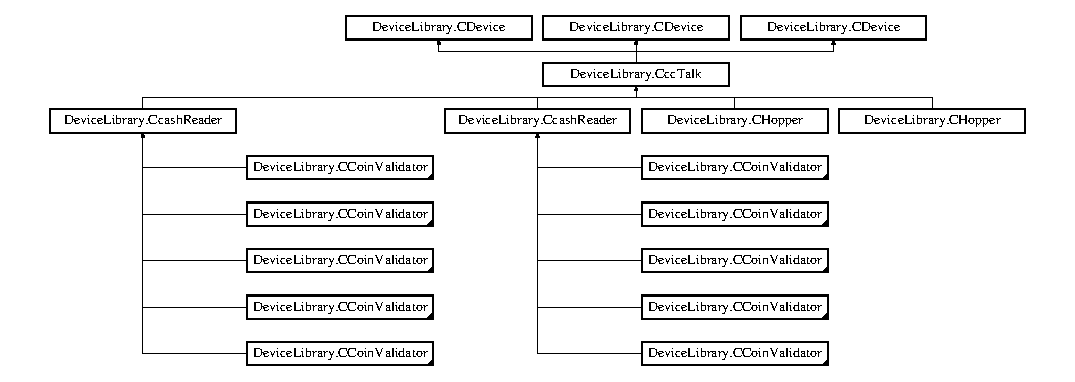
\includegraphics[height=4.691100cm]{class_device_library_1_1_ccc_talk}
\end{center}
\end{figure}
\subsection*{Public Types}
\begin{DoxyCompactItemize}
\item 
enum \mbox{\hyperlink{group___header_ga22f8eb6526627d4203e53ce7dbd3052a}{Header}} \+: byte \{ \newline
\mbox{\hyperlink{group___header_gga22f8eb6526627d4203e53ce7dbd3052aaf6daafc242a3bea0cfdf8deaac4cbdfe}{Header.\+F\+A\+C\+T\+O\+R\+Y\+S\+E\+T\+UP}} = 255, 
\mbox{\hyperlink{group___header_gga22f8eb6526627d4203e53ce7dbd3052aa28989b1e5d1316cb7695aa363f531a97}{Header.\+S\+I\+M\+P\+L\+E\+P\+O\+LL}} = 254, 
\mbox{\hyperlink{group___header_gga22f8eb6526627d4203e53ce7dbd3052aa909355816ff6e7e959619e23789f2227}{Header.\+A\+D\+D\+R\+E\+S\+S\+P\+O\+LL}} = 253, 
\mbox{\hyperlink{group___header_gga22f8eb6526627d4203e53ce7dbd3052aa44aba6ad436073d338560f89aa8f6154}{Header.\+A\+D\+D\+R\+E\+S\+S\+C\+L\+A\+SH}} = 252, 
\newline
\mbox{\hyperlink{group___header_gga22f8eb6526627d4203e53ce7dbd3052aa2dcd6749aa763943ba4b2f6b62962505}{Header.\+A\+D\+D\+R\+E\+S\+S\+C\+H\+A\+N\+GE}} = 251, 
\mbox{\hyperlink{group___header_gga22f8eb6526627d4203e53ce7dbd3052aa4ddfc0abc8dafde9a696ba71824c1f72}{Header.\+A\+D\+D\+R\+E\+S\+S\+R\+A\+N\+D\+OM}} = 250, 
\mbox{\hyperlink{group___header_gga22f8eb6526627d4203e53ce7dbd3052aa0b86a65dca9c484a7bde9fca38803f0b}{Header.\+R\+E\+Q\+U\+E\+S\+T\+V\+A\+R\+I\+A\+B\+L\+E\+S\+ET}} = 247, 
\mbox{\hyperlink{group___header_gga22f8eb6526627d4203e53ce7dbd3052aab513d3b7fc4b96e054937fb6fbbb0729}{Header.\+R\+E\+Q\+U\+E\+S\+T\+M\+A\+N\+U\+F\+A\+C\+T\+U\+R\+E\+R\+ID}} = 246, 
\newline
\mbox{\hyperlink{group___header_gga22f8eb6526627d4203e53ce7dbd3052aae7716221fdaec83804880e8765cf7d10}{Header.\+R\+E\+Q\+U\+E\+S\+T\+E\+Q\+U\+I\+P\+E\+M\+E\+N\+T\+C\+A\+T\+E\+G\+O\+R\+Y\+ID}} = 245, 
\mbox{\hyperlink{group___header_gga22f8eb6526627d4203e53ce7dbd3052aaaf384971e229ef28c276b9779bd81388}{Header.\+R\+E\+Q\+U\+E\+S\+T\+P\+R\+O\+D\+U\+C\+T\+C\+O\+DE}} = 244, 
\mbox{\hyperlink{group___header_gga22f8eb6526627d4203e53ce7dbd3052aa3227e2092fc0766e61a1a732de61062d}{Header.\+R\+E\+Q\+U\+E\+S\+T\+SN}} = 242, 
\mbox{\hyperlink{group___header_gga22f8eb6526627d4203e53ce7dbd3052aa7e17eee28297a1c7131d78d335dc3dc7}{Header.\+R\+E\+Q\+U\+E\+S\+T\+S\+W\+R\+EV}} = 241, 
\newline
\mbox{\hyperlink{group___header_gga22f8eb6526627d4203e53ce7dbd3052aa9163ec519df517704db337f07ea927d6}{Header.\+O\+P\+E\+R\+A\+T\+E\+M\+O\+T\+OR}} = 239, 
\mbox{\hyperlink{group___header_gga22f8eb6526627d4203e53ce7dbd3052aaf7401a2b001f90c26bb2be51b83799b3}{Header.\+R\+E\+A\+D\+O\+P\+T\+O\+S\+T\+A\+T\+ES}} = 236, 
\mbox{\hyperlink{group___header_gga22f8eb6526627d4203e53ce7dbd3052aa4236a0843d4f19fe52b9c493eb437802}{Header.\+E\+N\+T\+E\+R\+N\+E\+W\+P\+I\+N\+N\+U\+M\+B\+ER}} = 219, 
\mbox{\hyperlink{group___header_gga22f8eb6526627d4203e53ce7dbd3052aaf8106609f05a253f413197be056fba71}{Header.\+E\+N\+T\+E\+R\+P\+I\+N\+N\+U\+M\+B\+ER}} = 218, 
\newline
\mbox{\hyperlink{group___header_gga22f8eb6526627d4203e53ce7dbd3052aad598c36cca844abd31f22322ef8670c7}{Header.\+R\+E\+Q\+U\+E\+S\+T\+D\+A\+T\+A\+S\+T\+O\+R\+A\+G\+E\+A\+V\+A\+I\+L\+A\+B\+I\+L\+I\+TY}} = 216, 
\mbox{\hyperlink{group___header_gga22f8eb6526627d4203e53ce7dbd3052aaf4d3266005046022ff52ffa5c3f3f0c3}{Header.\+R\+E\+A\+D\+D\+A\+T\+A\+B\+L\+O\+CK}} = 215, 
\mbox{\hyperlink{group___header_gga22f8eb6526627d4203e53ce7dbd3052aaf42de9fb76d8e85f35c258b77e2ff02a}{Header.\+W\+R\+I\+T\+E\+D\+A\+T\+A\+B\+L\+O\+CK}} = 214, 
\mbox{\hyperlink{group___header_gga22f8eb6526627d4203e53ce7dbd3052aa3ea83e192f7d50bb0bd2b51a5f4883e1}{Header.\+R\+E\+Q\+U\+E\+S\+T\+B\+U\+I\+L\+D\+C\+O\+DE}} = 192, 
\newline
\mbox{\hyperlink{group___header_gga22f8eb6526627d4203e53ce7dbd3052aaaa233eaf5d8e09ef8ca6c3c120ee0388}{Header.\+R\+E\+Q\+U\+E\+S\+T\+B\+A\+S\+E\+Y\+E\+AR}} = 170, 
\mbox{\hyperlink{group___header_gga22f8eb6526627d4203e53ce7dbd3052aadd771b5014d8dfb2d691b886c0d0154c}{Header.\+R\+E\+Q\+U\+E\+S\+T\+A\+D\+D\+R\+E\+S\+S\+M\+O\+DE}} = 169, 
\mbox{\hyperlink{group___header_gga22f8eb6526627d4203e53ce7dbd3052aae924a1d3fed578124d2542b501b9d5be}{Header.\+M\+O\+D\+I\+F\+Y\+V\+A\+R\+I\+A\+B\+L\+E\+S\+ET}} = 165, 
\mbox{\hyperlink{group___header_gga22f8eb6526627d4203e53ce7dbd3052aa7179596553bfb00fe3a54fb1c4f46d2e}{Header.\+S\+W\+I\+T\+C\+H\+E\+N\+C\+R\+Y\+P\+T\+I\+O\+N\+C\+O\+DE}} = 137, 
\newline
\mbox{\hyperlink{group___header_gga22f8eb6526627d4203e53ce7dbd3052aa175f64a90ae2bf6edd145a17609268a1}{Header.\+S\+T\+O\+R\+E\+E\+N\+C\+R\+Y\+P\+T\+I\+O\+N\+C\+O\+DE}} =136, 
\mbox{\hyperlink{group___header_gga22f8eb6526627d4203e53ce7dbd3052aa802706a9238e2928077f97736854bad4}{Header.\+B\+U\+SY}} = 6, 
\mbox{\hyperlink{group___header_gga22f8eb6526627d4203e53ce7dbd3052aa3860aef5aa76641c6959d1a5de94b216}{Header.\+N\+AK}} = 5, 
\mbox{\hyperlink{group___header_gga22f8eb6526627d4203e53ce7dbd3052aa233ae98d8a18c499eb4b798360aa02ef}{Header.\+R\+E\+Q\+U\+E\+S\+T\+C\+O\+M\+M\+S\+R\+E\+V\+I\+S\+I\+ON}} = 4, 
\newline
\mbox{\hyperlink{group___header_gga22f8eb6526627d4203e53ce7dbd3052aafb4cfb0ac631109fa01bdbd70ba8e166}{Header.\+C\+L\+E\+A\+R\+C\+O\+M\+M\+S\+S\+T\+A\+T\+U\+S\+V\+A\+R\+I\+A\+B\+L\+ES}} = 3, 
\mbox{\hyperlink{group___header_gga22f8eb6526627d4203e53ce7dbd3052aaacaa18d8173ad7149b61185d29c4f3bb}{Header.\+R\+E\+Q\+U\+E\+S\+T\+C\+O\+M\+M\+S\+S\+T\+A\+T\+U\+S\+V\+A\+R\+I\+A\+B\+L\+ES}} = 2, 
\mbox{\hyperlink{group___header_gga22f8eb6526627d4203e53ce7dbd3052aab87acc3ce509b6e2b20a564607eb06d8}{Header.\+R\+E\+S\+E\+T\+D\+E\+V\+I\+CE}} = 1
 \}
\begin{DoxyCompactList}\small\item\em Enumération des headers communs à tous les périphériques cc\+Talk. \end{DoxyCompactList}\item 
enum \mbox{\hyperlink{group___erreur_ga179570d2d8f6f95d52ccafb98d20c790}{Self\+Test\+Result}} \{ \newline
\mbox{\hyperlink{group___erreur_gga179570d2d8f6f95d52ccafb98d20c790ae0aa021e21dddbd6d8cecec71e9cf564}{Self\+Test\+Result.\+OK}} = 0, 
\mbox{\hyperlink{group___erreur_gga179570d2d8f6f95d52ccafb98d20c790a82728633b7a7c49ed136d5c3aa605861}{Self\+Test\+Result.\+E\+R\+R\+O\+R\+C\+H\+E\+C\+K\+S\+UM}} = 1, 
\mbox{\hyperlink{group___erreur_gga179570d2d8f6f95d52ccafb98d20c790aa4c8c213e52281611bbc2d726f23959a}{Self\+Test\+Result.\+E\+R\+R\+O\+R\+C\+O\+I\+L\+M\+E\+A\+S\+U\+R\+E\+M\+E\+NT}} = 2, 
\mbox{\hyperlink{group___erreur_gga179570d2d8f6f95d52ccafb98d20c790a4ef2b74a0cc5d6393ce608c54b1861f0}{Self\+Test\+Result.\+E\+R\+R\+O\+R\+C\+R\+E\+D\+I\+T\+S\+E\+N\+S\+OR}} = 3, 
\newline
\mbox{\hyperlink{group___erreur_gga179570d2d8f6f95d52ccafb98d20c790a45609713be805992c730f031ff8f54ca}{Self\+Test\+Result.\+E\+R\+R\+O\+R\+P\+I\+E\+Z\+O\+S\+E\+N\+S\+OR}} =4, 
\mbox{\hyperlink{group___erreur_gga179570d2d8f6f95d52ccafb98d20c790abe71e29807fc8e2627732f98b625dd63}{Self\+Test\+Result.\+E\+R\+R\+O\+R\+R\+E\+F\+L\+E\+C\+T\+I\+V\+E\+S\+E\+N\+S\+OR}} = 5, 
\mbox{\hyperlink{group___erreur_gga179570d2d8f6f95d52ccafb98d20c790a06c7dd879850f00fcce4a46b4f0f4baf}{Self\+Test\+Result.\+E\+R\+R\+O\+R\+D\+I\+A\+M\+E\+T\+E\+R\+S\+E\+N\+S\+OR}} = 6, 
\mbox{\hyperlink{group___erreur_gga179570d2d8f6f95d52ccafb98d20c790afd502fbfb573105b14080349c146d0da}{Self\+Test\+Result.\+E\+R\+R\+O\+R\+O\+N\+W\+A\+K\+E\+U\+P\+S\+E\+N\+S\+OR}} = 7, 
\newline
\mbox{\hyperlink{group___erreur_gga179570d2d8f6f95d52ccafb98d20c790afc13d39d093e34a09c0a0314e20048ee}{Self\+Test\+Result.\+E\+R\+R\+O\+R\+E\+X\+I\+T\+S\+E\+N\+S\+OR}} = 8, 
\mbox{\hyperlink{group___erreur_gga179570d2d8f6f95d52ccafb98d20c790a0c4861a28780ce88a698758dde79d029}{Self\+Test\+Result.\+N\+V\+R\+A\+M\+C\+H\+E\+C\+K\+S\+UM}} = 9, 
\mbox{\hyperlink{group___erreur_gga179570d2d8f6f95d52ccafb98d20c790adbe12f65a0cd3985f952f395ee8ff65d}{Self\+Test\+Result.\+E\+R\+R\+O\+R\+K\+E\+Y\+P\+AD}} = 14, 
\mbox{\hyperlink{group___erreur_gga179570d2d8f6f95d52ccafb98d20c790a543b5fd5ff186ca8f13b355ac0edc446}{Self\+Test\+Result.\+E\+R\+R\+O\+R\+B\+U\+T\+T\+ON}} = 15, 
\newline
\mbox{\hyperlink{group___erreur_gga179570d2d8f6f95d52ccafb98d20c790a921d7ae7f037c6fc8b9dc65cd11562eb}{Self\+Test\+Result.\+E\+R\+R\+O\+R\+D\+I\+S\+P\+L\+AY}} = 16, 
\mbox{\hyperlink{group___erreur_gga179570d2d8f6f95d52ccafb98d20c790a07bcbb954c85682dc9897bbce2f4465c}{Self\+Test\+Result.\+C\+O\+I\+N\+A\+U\+D\+I\+T\+E\+R\+R\+OR}} = 17, 
\mbox{\hyperlink{group___erreur_gga179570d2d8f6f95d52ccafb98d20c790ad7821dc039e60525debddf85ce046024}{Self\+Test\+Result.\+E\+R\+R\+O\+R\+O\+N\+R\+E\+J\+E\+C\+T\+S\+E\+N\+S\+OR}} = 18, 
\mbox{\hyperlink{group___erreur_gga179570d2d8f6f95d52ccafb98d20c790ac83370dde56d0f3b5313682a04ad7670}{Self\+Test\+Result.\+E\+R\+R\+O\+R\+O\+N\+C\+O\+I\+N\+R\+E\+T\+U\+R\+N\+M\+E\+CH}} = 19, 
\newline
\mbox{\hyperlink{group___erreur_gga179570d2d8f6f95d52ccafb98d20c790af032d38e084b27c8bc8fc272c9b1d9ad}{Self\+Test\+Result.\+E\+R\+R\+O\+R\+C\+O\+S\+M\+E\+CH}} = 20, 
\mbox{\hyperlink{group___erreur_gga179570d2d8f6f95d52ccafb98d20c790ae1ae427e9a19c79560a4298b49ad7aad}{Self\+Test\+Result.\+E\+R\+R\+O\+R\+R\+IM}} = 21, 
\mbox{\hyperlink{group___erreur_gga179570d2d8f6f95d52ccafb98d20c790ac4c0edc9040440850d32e07b63e99e71}{Self\+Test\+Result.\+E\+R\+R\+O\+R\+T\+H\+E\+R\+M\+I\+S\+T\+OR}} = 22, 
\mbox{\hyperlink{group___erreur_gga179570d2d8f6f95d52ccafb98d20c790ae48b541e05c3de25f7c19f32e905421e}{Self\+Test\+Result.\+E\+R\+R\+O\+R\+M\+O\+T\+OR}} = 23, 
\newline
\mbox{\hyperlink{group___erreur_gga179570d2d8f6f95d52ccafb98d20c790a2b062c09a10f709598a9a3b22349fb13}{Self\+Test\+Result.\+E\+R\+R\+O\+R\+P\+A\+Y\+O\+U\+T\+S\+E\+N\+S\+OR}} = 26, 
\mbox{\hyperlink{group___erreur_gga179570d2d8f6f95d52ccafb98d20c790aeecc3076ef1f092d654d0572732d8fae}{Self\+Test\+Result.\+E\+R\+R\+O\+R\+L\+E\+V\+E\+L\+S\+E\+N\+S\+OR}} = 27, 
\mbox{\hyperlink{group___erreur_gga179570d2d8f6f95d52ccafb98d20c790a188f9098e533155473b37511e1608b41}{Self\+Test\+Result.\+E\+R\+R\+O\+R\+D\+A\+T\+A\+B\+L\+O\+C\+K\+C\+H\+E\+C\+S\+UM}} = 30, 
\mbox{\hyperlink{group___erreur_gga179570d2d8f6f95d52ccafb98d20c790a98fbededc5219d4233faf4f4dfecb8b8}{Self\+Test\+Result.\+E\+R\+R\+O\+R\+I\+N\+T\+E\+R\+N\+A\+L\+C\+OM}} = 32, 
\newline
\mbox{\hyperlink{group___erreur_gga179570d2d8f6f95d52ccafb98d20c790a5b756a3101dde017415ebfb924123352}{Self\+Test\+Result.\+E\+R\+R\+O\+R\+P\+O\+W\+E\+R\+S\+U\+P\+P\+LY}} = 33, 
\mbox{\hyperlink{group___erreur_gga179570d2d8f6f95d52ccafb98d20c790ac7f53b99909b3d23ed52c89a2c4251a1}{Self\+Test\+Result.\+E\+R\+R\+O\+R\+T\+E\+MP}} = 34, 
\mbox{\hyperlink{group___erreur_gga179570d2d8f6f95d52ccafb98d20c790a6ad548781f29d837560c33c17f76bcbf}{Self\+Test\+Result.\+E\+R\+R\+O\+R\+D\+CE}} = 35, 
\mbox{\hyperlink{group___erreur_gga179570d2d8f6f95d52ccafb98d20c790afd6e0d70f810e3936dca24e2c9e88366}{Self\+Test\+Result.\+E\+R\+R\+O\+R\+B\+V\+S\+E\+N\+S\+OR}} = 36, 
\newline
\mbox{\hyperlink{group___erreur_gga179570d2d8f6f95d52ccafb98d20c790ae2320146778712445e1bda765a3827e4}{Self\+Test\+Result.\+E\+R\+R\+O\+R\+B\+V\+T\+R\+A\+N\+S\+P\+O\+RT}} = 37, 
\mbox{\hyperlink{group___erreur_gga179570d2d8f6f95d52ccafb98d20c790a80572a1d9e446f50c294b206b8724b87}{Self\+Test\+Result.\+E\+R\+R\+O\+R\+S\+T\+A\+C\+K\+ER}} = 38, 
\mbox{\hyperlink{group___erreur_gga179570d2d8f6f95d52ccafb98d20c790a2cd8c522b6febe25beae6dd244557faa}{Self\+Test\+Result.\+B\+I\+L\+L\+J\+A\+M\+M\+ED}} = 39, 
\mbox{\hyperlink{group___erreur_gga179570d2d8f6f95d52ccafb98d20c790aae684db02df998c0503f38b901302cb3}{Self\+Test\+Result.\+E\+R\+R\+O\+R\+T\+E\+S\+T\+R\+AM}} = 40, 
\newline
\mbox{\hyperlink{group___erreur_gga179570d2d8f6f95d52ccafb98d20c790a8cc746f58e0de79fe992db40e266fc89}{Self\+Test\+Result.\+E\+R\+R\+O\+R\+S\+T\+R\+I\+N\+G\+S\+E\+N\+S\+OR}} = 41, 
\mbox{\hyperlink{group___erreur_gga179570d2d8f6f95d52ccafb98d20c790a233e99ec360a60f14d17ad4e088398ee}{Self\+Test\+Result.\+E\+R\+R\+O\+R\+A\+C\+C\+E\+P\+T\+G\+A\+T\+E\+O\+P\+EN}} = 42, 
\mbox{\hyperlink{group___erreur_gga179570d2d8f6f95d52ccafb98d20c790aef82674b077701d481db50067a39dadf}{Self\+Test\+Result.\+E\+R\+R\+O\+R\+A\+C\+C\+E\+P\+T\+G\+A\+T\+E\+C\+L\+O\+SE}} = 43, 
\mbox{\hyperlink{group___erreur_gga179570d2d8f6f95d52ccafb98d20c790a3f14cb8d189627ff94c09e37485d5e4d}{Self\+Test\+Result.\+S\+T\+A\+C\+K\+E\+R\+M\+I\+S\+S\+I\+NG}} = 44, 
\newline
\mbox{\hyperlink{group___erreur_gga179570d2d8f6f95d52ccafb98d20c790a3753cc88724c8753903f0c00fb2a70ec}{Self\+Test\+Result.\+S\+T\+A\+C\+K\+E\+R\+F\+U\+LL}} = 45, 
\mbox{\hyperlink{group___erreur_gga179570d2d8f6f95d52ccafb98d20c790a64b9b8a79fbd8e516d73d947f23789f5}{Self\+Test\+Result.\+E\+R\+R\+O\+R\+E\+R\+A\+S\+E\+F\+L\+A\+S\+H\+M\+EM}} = 46, 
\mbox{\hyperlink{group___erreur_gga179570d2d8f6f95d52ccafb98d20c790a47a8bac7b81fb8860aa60a0c27abfa9e}{Self\+Test\+Result.\+E\+R\+R\+O\+R\+W\+R\+I\+T\+E\+F\+L\+A\+S\+H\+M\+EM}} = 47, 
\mbox{\hyperlink{group___erreur_gga179570d2d8f6f95d52ccafb98d20c790a6971f8ba4fd456e6028307790060416e}{Self\+Test\+Result.\+E\+R\+R\+O\+R\+S\+L\+A\+V\+E\+D\+E\+V\+I\+CE}} = 48, 
\newline
\mbox{\hyperlink{group___erreur_gga179570d2d8f6f95d52ccafb98d20c790a5f416c3c0f2315e101772fb4afa19159}{Self\+Test\+Result.\+E\+R\+R\+O\+R\+O\+P\+T\+O\+S\+E\+N\+S\+OR}} = 49, 
\mbox{\hyperlink{group___erreur_gga179570d2d8f6f95d52ccafb98d20c790abc304fceb86fed05a9c1480ae161e105}{Self\+Test\+Result.\+E\+R\+R\+O\+R\+B\+A\+T\+T\+E\+RY}} = 50, 
\mbox{\hyperlink{group___erreur_gga179570d2d8f6f95d52ccafb98d20c790a2e7bbba7a345ba75be6d7afa5099e4b2}{Self\+Test\+Result.\+E\+R\+R\+O\+R\+D\+O\+O\+R\+O\+P\+EN}} = 51, 
\mbox{\hyperlink{group___erreur_gga179570d2d8f6f95d52ccafb98d20c790aaccb25b7024f8a8457070b5f219cc8cb}{Self\+Test\+Result.\+E\+R\+R\+O\+R\+M\+I\+C\+R\+O\+S\+W\+I\+T\+CH}} = 52, 
\newline
\mbox{\hyperlink{group___erreur_gga179570d2d8f6f95d52ccafb98d20c790a452e48f2270532eeb8a7d1a08b2bffa9}{Self\+Test\+Result.\+E\+R\+R\+O\+R\+R\+TC}} = 53, 
\mbox{\hyperlink{group___erreur_gga179570d2d8f6f95d52ccafb98d20c790a17067ea1451de42b4bf3752122768b55}{Self\+Test\+Result.\+E\+R\+R\+O\+R\+FW}} = 54, 
\mbox{\hyperlink{group___erreur_gga179570d2d8f6f95d52ccafb98d20c790a742a02b5a464f1e436fe1ce890b537a8}{Self\+Test\+Result.\+E\+R\+R\+O\+R\+I\+N\+IT}} = 55, 
\mbox{\hyperlink{group___erreur_gga179570d2d8f6f95d52ccafb98d20c790a83c9f2a51be490451be24a146c1d808b}{Self\+Test\+Result.\+E\+R\+R\+O\+R\+C\+U\+R\+R\+E\+N\+T\+S\+U\+P\+P\+LY}} = 56, 
\newline
\mbox{\hyperlink{group___erreur_gga179570d2d8f6f95d52ccafb98d20c790ad7e9c71913cffcaabd565eaee9cf52b8}{Self\+Test\+Result.\+F\+O\+R\+C\+E\+B\+O\+O\+T\+L\+O\+A\+D\+E\+R\+M\+O\+DE}} = 57, 
\mbox{\hyperlink{group___erreur_gga179570d2d8f6f95d52ccafb98d20c790a5fd22f0fcfa09dee2ad29a0653ed7963}{Self\+Test\+Result.\+C\+O\+I\+N\+J\+AM}} = 253, 
\mbox{\hyperlink{group___erreur_gga179570d2d8f6f95d52ccafb98d20c790acaf20830f50dde044b5d55b78bd4ccfe}{Self\+Test\+Result.\+D\+I\+S\+K\+B\+L\+O\+C\+K\+ED}} = 254, 
\mbox{\hyperlink{group___erreur_gga179570d2d8f6f95d52ccafb98d20c790a17871c6d9d47f1e52c2681e98a1a9143}{Self\+Test\+Result.\+E\+R\+R\+O\+R\+U\+N\+K\+N\+OW}} = 255
 \}
\begin{DoxyCompactList}\small\item\em Liste des fautes possibles retournées par un self test. \end{DoxyCompactList}\end{DoxyCompactItemize}
\subsection*{Public Member Functions}
\begin{DoxyCompactItemize}
\item 
\mbox{\hyperlink{class_device_library_1_1_ccc_talk_acb6f8e8dcdfa88d9cdc5b3ebf1ea0e90}{Ccc\+Talk}} ()
\begin{DoxyCompactList}\small\item\em Construteur de la class \end{DoxyCompactList}\item 
bool \mbox{\hyperlink{class_device_library_1_1_ccc_talk_ab986f5ca49ce60e90442b54682f34b62}{Is\+Cmdcc\+Talk\+Sended}} (\mbox{\hyperlink{namespace_device_library_a4ca177654b0e196e5a5f5275fb4ea5ee}{Default\+Devices\+Address}} Peripherique, object Commande, byte Len\+Param, byte\mbox{[}$\,$\mbox{]} Parameter, object answer)
\begin{DoxyCompactList}\small\item\em Envoie une commande et recoit la réponse \end{DoxyCompactList}\item 
bool \mbox{\hyperlink{class_device_library_1_1_ccc_talk_a9069f40563639ecc85dac7dd9c212cee}{Reset\+Device}} ()
\begin{DoxyCompactList}\small\item\em State\+Reset software du périphérique. \end{DoxyCompactList}\end{DoxyCompactItemize}
\subsection*{Static Public Member Functions}
\begin{DoxyCompactItemize}
\item 
static void \mbox{\hyperlink{class_device_library_1_1_ccc_talk_a9e6bea86795ec29fde4e6071256eff76}{Reset\+Counters}} ()
\begin{DoxyCompactList}\small\item\em Remise à zéro des compteurs \end{DoxyCompactList}\end{DoxyCompactItemize}
\subsection*{Public Attributes}
\begin{DoxyCompactItemize}
\item 
const string \mbox{\hyperlink{class_device_library_1_1_ccc_talk_ad5c6d1287d0c049bdbf4fda8cb19c1ef}{file\+Counter\+Name}} = \char`\"{}Counters.\+mtr\char`\"{}
\begin{DoxyCompactList}\small\item\em Nom du fichier contenant les compteurs. \end{DoxyCompactList}\end{DoxyCompactItemize}
\subsection*{Static Public Attributes}
\begin{DoxyCompactItemize}
\item 
static Serial\+Port \mbox{\hyperlink{class_device_library_1_1_ccc_talk_acda9f65e6498cce0d3e51ad1b587ede4}{Port\+Serie}}
\begin{DoxyCompactList}\small\item\em Port série utilisée par le bus cc\+Talk \end{DoxyCompactList}\item 
static Mutex \mbox{\hyperlink{class_device_library_1_1_ccc_talk_aabbbe46d911d826c39712d8aecd10786}{mutex\+C\+C\+Talk}} = new Mutex()
\item 
static \mbox{\hyperlink{class_device_library_1_1_ccoins_counters}{Ccoins\+Counters}} \mbox{\hyperlink{class_device_library_1_1_ccc_talk_a3810c0aa448865e19afff87a946fee5d}{counters}}
\begin{DoxyCompactList}\small\item\em Compteurs \end{DoxyCompactList}\item 
static Stream \mbox{\hyperlink{class_device_library_1_1_ccc_talk_ada638d9c9c453de40591720409ef4b54}{counters\+File}}
\begin{DoxyCompactList}\small\item\em Fichier des compteurs. \end{DoxyCompactList}\item 
static Binary\+Formatter \mbox{\hyperlink{class_device_library_1_1_ccc_talk_aa8d3dfce2d2f9f1f2c9ca524d1fbcc8f}{counter\+Serializer}}
\end{DoxyCompactItemize}
\subsection*{Protected Member Functions}
\begin{DoxyCompactItemize}
\item 
byte \mbox{\hyperlink{class_device_library_1_1_ccc_talk_a5f67f62cb03d573225712813348408ad}{Get\+Byte}} (object header)
\begin{DoxyCompactList}\small\item\em Lit un octet dans le périphérique \end{DoxyCompactList}\end{DoxyCompactItemize}
\subsection*{Static Protected Attributes}
\begin{DoxyCompactItemize}
\item 
static object \mbox{\hyperlink{class_device_library_1_1_ccc_talk_a43ca834802480b1171030f7ad063c559}{verrou}} = new object()
\begin{DoxyCompactList}\small\item\em Verrou du thread \end{DoxyCompactList}\end{DoxyCompactItemize}
\subsection*{Properties}
\begin{DoxyCompactItemize}
\item 
\mbox{\hyperlink{namespace_device_library_a4ca177654b0e196e5a5f5275fb4ea5ee}{Default\+Devices\+Address}} \mbox{\hyperlink{class_device_library_1_1_ccc_talk_aff70a9d7d6adc3e95593259d17751cb8}{Device\+Address}}\hspace{0.3cm}{\ttfamily  \mbox{[}get, set\mbox{]}}
\begin{DoxyCompactList}\small\item\em Adresse du périphérique. \end{DoxyCompactList}\item 
override string \mbox{\hyperlink{class_device_library_1_1_ccc_talk_a73a84f7534b5b9ff129897b86d483f48}{Manufacturer}}\hspace{0.3cm}{\ttfamily  \mbox{[}get\mbox{]}}
\begin{DoxyCompactList}\small\item\em Retourne l\textquotesingle{}identifiant du fabricant. \end{DoxyCompactList}\item 
string \mbox{\hyperlink{class_device_library_1_1_ccc_talk_ae73c18703dae000c9f725a44fae17f1a}{Build\+Code}}\hspace{0.3cm}{\ttfamily  \mbox{[}get\mbox{]}}
\begin{DoxyCompactList}\small\item\em Code de production du périphérique. \end{DoxyCompactList}\item 
override string \mbox{\hyperlink{class_device_library_1_1_ccc_talk_abd92229809b4474129b15e638fd56da7}{Product\+Code}}\hspace{0.3cm}{\ttfamily  \mbox{[}get\mbox{]}}
\begin{DoxyCompactList}\small\item\em Code produit du périphérique. \end{DoxyCompactList}\item 
string \mbox{\hyperlink{class_device_library_1_1_ccc_talk_a3cb80b7a82cc363e0dcefd1f31ced8a2}{Equipement\+Category}}\hspace{0.3cm}{\ttfamily  \mbox{[}get\mbox{]}}
\begin{DoxyCompactList}\small\item\em Code produit du périphérique. \end{DoxyCompactList}\item 
override int \mbox{\hyperlink{class_device_library_1_1_ccc_talk_a6b615dcccbe32e3c9166b0fdb0a74236}{Serial\+Number}}\hspace{0.3cm}{\ttfamily  \mbox{[}get\mbox{]}}
\begin{DoxyCompactList}\small\item\em Retourne le numéro de série du pelicano \end{DoxyCompactList}\item 
string \mbox{\hyperlink{class_device_library_1_1_ccc_talk_a687a695bef6d7f25f8fe7148948d04bc}{S\+W\+Rev}}\hspace{0.3cm}{\ttfamily  \mbox{[}get\mbox{]}}
\begin{DoxyCompactList}\small\item\em Retourne la révision software \end{DoxyCompactList}\item 
string \mbox{\hyperlink{class_device_library_1_1_ccc_talk_af78c9d598eaebc02a257d52353ab257c}{Comms\+Revision}}\hspace{0.3cm}{\ttfamily  \mbox{[}get\mbox{]}}
\item 
bool \mbox{\hyperlink{class_device_library_1_1_ccc_talk_a576e09f74dc509dcd7919eceae9cc7de}{Simple\+Poll}}\hspace{0.3cm}{\ttfamily  \mbox{[}get\mbox{]}}
\begin{DoxyCompactList}\small\item\em Simple poll du périphérique. \end{DoxyCompactList}\item 
virtual byte \mbox{\hyperlink{class_device_library_1_1_ccc_talk_a4ea55bd396398405345e50cb699c0ead}{Opto\+States}}\hspace{0.3cm}{\ttfamily  \mbox{[}get\mbox{]}}
\end{DoxyCompactItemize}


\subsection{Detailed Description}
Class cc\+Talk 



\subsection{Constructor \& Destructor Documentation}
\mbox{\Hypertarget{class_device_library_1_1_ccc_talk_acb6f8e8dcdfa88d9cdc5b3ebf1ea0e90}\label{class_device_library_1_1_ccc_talk_acb6f8e8dcdfa88d9cdc5b3ebf1ea0e90}} 
\index{Device\+Library\+::\+Ccc\+Talk@{Device\+Library\+::\+Ccc\+Talk}!Ccc\+Talk@{Ccc\+Talk}}
\index{Ccc\+Talk@{Ccc\+Talk}!Device\+Library\+::\+Ccc\+Talk@{Device\+Library\+::\+Ccc\+Talk}}
\subsubsection{\texorpdfstring{Ccc\+Talk()}{CccTalk()}}
{\footnotesize\ttfamily Device\+Library.\+Ccc\+Talk.\+Ccc\+Talk (\begin{DoxyParamCaption}{ }\end{DoxyParamCaption})\hspace{0.3cm}{\ttfamily [inline]}}



Construteur de la class 



\subsection{Member Function Documentation}
\mbox{\Hypertarget{class_device_library_1_1_ccc_talk_a5f67f62cb03d573225712813348408ad}\label{class_device_library_1_1_ccc_talk_a5f67f62cb03d573225712813348408ad}} 
\index{Device\+Library\+::\+Ccc\+Talk@{Device\+Library\+::\+Ccc\+Talk}!Get\+Byte@{Get\+Byte}}
\index{Get\+Byte@{Get\+Byte}!Device\+Library\+::\+Ccc\+Talk@{Device\+Library\+::\+Ccc\+Talk}}
\subsubsection{\texorpdfstring{Get\+Byte()}{GetByte()}}
{\footnotesize\ttfamily byte Device\+Library.\+Ccc\+Talk.\+Get\+Byte (\begin{DoxyParamCaption}\item[{object}]{header }\end{DoxyParamCaption})\hspace{0.3cm}{\ttfamily [inline]}, {\ttfamily [protected]}}



Lit un octet dans le périphérique 


\begin{DoxyParams}{Parameters}
{\em header} & Header de la requête\\
\hline
\end{DoxyParams}


La valeur de l\textquotesingle{}octet retourné est 255

\begin{DoxyReturn}{Returns}
la valeur de l\textquotesingle{}octet demandé
\end{DoxyReturn}
\mbox{\Hypertarget{class_device_library_1_1_ccc_talk_ab986f5ca49ce60e90442b54682f34b62}\label{class_device_library_1_1_ccc_talk_ab986f5ca49ce60e90442b54682f34b62}} 
\index{Device\+Library\+::\+Ccc\+Talk@{Device\+Library\+::\+Ccc\+Talk}!Is\+Cmdcc\+Talk\+Sended@{Is\+Cmdcc\+Talk\+Sended}}
\index{Is\+Cmdcc\+Talk\+Sended@{Is\+Cmdcc\+Talk\+Sended}!Device\+Library\+::\+Ccc\+Talk@{Device\+Library\+::\+Ccc\+Talk}}
\subsubsection{\texorpdfstring{Is\+Cmdcc\+Talk\+Sended()}{IsCmdccTalkSended()}}
{\footnotesize\ttfamily bool Device\+Library.\+Ccc\+Talk.\+Is\+Cmdcc\+Talk\+Sended (\begin{DoxyParamCaption}\item[{\mbox{\hyperlink{namespace_device_library_a4ca177654b0e196e5a5f5275fb4ea5ee}{Default\+Devices\+Address}}}]{Peripherique,  }\item[{object}]{Commande,  }\item[{byte}]{Len\+Param,  }\item[{byte \mbox{[}$\,$\mbox{]}}]{Parameter,  }\item[{object}]{answer }\end{DoxyParamCaption})\hspace{0.3cm}{\ttfamily [inline]}}



Envoie une commande et recoit la réponse 


\begin{DoxyParams}{Parameters}
{\em Peripherique} & Adresse du périphérique\\
\hline
{\em Commande} & Header de la commande envoyée\\
\hline
{\em Len\+Param} & Longeur des paramètres\\
\hline
{\em Parameter} & Buffer des paramètres\\
\hline
{\em answer} & Objet contenant les paramètres de retour le cas échéant\\
\hline
\end{DoxyParams}
\begin{DoxyReturn}{Returns}

\end{DoxyReturn}
\mbox{\Hypertarget{class_device_library_1_1_ccc_talk_a9e6bea86795ec29fde4e6071256eff76}\label{class_device_library_1_1_ccc_talk_a9e6bea86795ec29fde4e6071256eff76}} 
\index{Device\+Library\+::\+Ccc\+Talk@{Device\+Library\+::\+Ccc\+Talk}!Reset\+Counters@{Reset\+Counters}}
\index{Reset\+Counters@{Reset\+Counters}!Device\+Library\+::\+Ccc\+Talk@{Device\+Library\+::\+Ccc\+Talk}}
\subsubsection{\texorpdfstring{Reset\+Counters()}{ResetCounters()}}
{\footnotesize\ttfamily static void Device\+Library.\+Ccc\+Talk.\+Reset\+Counters (\begin{DoxyParamCaption}{ }\end{DoxyParamCaption})\hspace{0.3cm}{\ttfamily [inline]}, {\ttfamily [static]}}



Remise à zéro des compteurs 

\mbox{\Hypertarget{class_device_library_1_1_ccc_talk_a9069f40563639ecc85dac7dd9c212cee}\label{class_device_library_1_1_ccc_talk_a9069f40563639ecc85dac7dd9c212cee}} 
\index{Device\+Library\+::\+Ccc\+Talk@{Device\+Library\+::\+Ccc\+Talk}!Reset\+Device@{Reset\+Device}}
\index{Reset\+Device@{Reset\+Device}!Device\+Library\+::\+Ccc\+Talk@{Device\+Library\+::\+Ccc\+Talk}}
\subsubsection{\texorpdfstring{Reset\+Device()}{ResetDevice()}}
{\footnotesize\ttfamily bool Device\+Library.\+Ccc\+Talk.\+Reset\+Device (\begin{DoxyParamCaption}{ }\end{DoxyParamCaption})\hspace{0.3cm}{\ttfamily [inline]}}



State\+Reset software du périphérique. 



\subsection{Member Data Documentation}
\mbox{\Hypertarget{class_device_library_1_1_ccc_talk_a3810c0aa448865e19afff87a946fee5d}\label{class_device_library_1_1_ccc_talk_a3810c0aa448865e19afff87a946fee5d}} 
\index{Device\+Library\+::\+Ccc\+Talk@{Device\+Library\+::\+Ccc\+Talk}!counters@{counters}}
\index{counters@{counters}!Device\+Library\+::\+Ccc\+Talk@{Device\+Library\+::\+Ccc\+Talk}}
\subsubsection{\texorpdfstring{counters}{counters}}
{\footnotesize\ttfamily \mbox{\hyperlink{class_device_library_1_1_ccoins_counters}{Ccoins\+Counters}} Device\+Library.\+Ccc\+Talk.\+counters\hspace{0.3cm}{\ttfamily [static]}}



Compteurs 

\mbox{\Hypertarget{class_device_library_1_1_ccc_talk_aa8d3dfce2d2f9f1f2c9ca524d1fbcc8f}\label{class_device_library_1_1_ccc_talk_aa8d3dfce2d2f9f1f2c9ca524d1fbcc8f}} 
\index{Device\+Library\+::\+Ccc\+Talk@{Device\+Library\+::\+Ccc\+Talk}!counter\+Serializer@{counter\+Serializer}}
\index{counter\+Serializer@{counter\+Serializer}!Device\+Library\+::\+Ccc\+Talk@{Device\+Library\+::\+Ccc\+Talk}}
\subsubsection{\texorpdfstring{counter\+Serializer}{counterSerializer}}
{\footnotesize\ttfamily Binary\+Formatter Device\+Library.\+Ccc\+Talk.\+counter\+Serializer\hspace{0.3cm}{\ttfamily [static]}}





\mbox{\Hypertarget{class_device_library_1_1_ccc_talk_ada638d9c9c453de40591720409ef4b54}\label{class_device_library_1_1_ccc_talk_ada638d9c9c453de40591720409ef4b54}} 
\index{Device\+Library\+::\+Ccc\+Talk@{Device\+Library\+::\+Ccc\+Talk}!counters\+File@{counters\+File}}
\index{counters\+File@{counters\+File}!Device\+Library\+::\+Ccc\+Talk@{Device\+Library\+::\+Ccc\+Talk}}
\subsubsection{\texorpdfstring{counters\+File}{countersFile}}
{\footnotesize\ttfamily Stream Device\+Library.\+Ccc\+Talk.\+counters\+File\hspace{0.3cm}{\ttfamily [static]}}



Fichier des compteurs. 

\mbox{\Hypertarget{class_device_library_1_1_ccc_talk_ad5c6d1287d0c049bdbf4fda8cb19c1ef}\label{class_device_library_1_1_ccc_talk_ad5c6d1287d0c049bdbf4fda8cb19c1ef}} 
\index{Device\+Library\+::\+Ccc\+Talk@{Device\+Library\+::\+Ccc\+Talk}!file\+Counter\+Name@{file\+Counter\+Name}}
\index{file\+Counter\+Name@{file\+Counter\+Name}!Device\+Library\+::\+Ccc\+Talk@{Device\+Library\+::\+Ccc\+Talk}}
\subsubsection{\texorpdfstring{file\+Counter\+Name}{fileCounterName}}
{\footnotesize\ttfamily const string Device\+Library.\+Ccc\+Talk.\+file\+Counter\+Name = \char`\"{}Counters.\+mtr\char`\"{}}



Nom du fichier contenant les compteurs. 

\mbox{\Hypertarget{class_device_library_1_1_ccc_talk_aabbbe46d911d826c39712d8aecd10786}\label{class_device_library_1_1_ccc_talk_aabbbe46d911d826c39712d8aecd10786}} 
\index{Device\+Library\+::\+Ccc\+Talk@{Device\+Library\+::\+Ccc\+Talk}!mutex\+C\+C\+Talk@{mutex\+C\+C\+Talk}}
\index{mutex\+C\+C\+Talk@{mutex\+C\+C\+Talk}!Device\+Library\+::\+Ccc\+Talk@{Device\+Library\+::\+Ccc\+Talk}}
\subsubsection{\texorpdfstring{mutex\+C\+C\+Talk}{mutexCCTalk}}
{\footnotesize\ttfamily Mutex Device\+Library.\+Ccc\+Talk.\+mutex\+C\+C\+Talk = new Mutex()\hspace{0.3cm}{\ttfamily [static]}}





\mbox{\Hypertarget{class_device_library_1_1_ccc_talk_acda9f65e6498cce0d3e51ad1b587ede4}\label{class_device_library_1_1_ccc_talk_acda9f65e6498cce0d3e51ad1b587ede4}} 
\index{Device\+Library\+::\+Ccc\+Talk@{Device\+Library\+::\+Ccc\+Talk}!Port\+Serie@{Port\+Serie}}
\index{Port\+Serie@{Port\+Serie}!Device\+Library\+::\+Ccc\+Talk@{Device\+Library\+::\+Ccc\+Talk}}
\subsubsection{\texorpdfstring{Port\+Serie}{PortSerie}}
{\footnotesize\ttfamily Serial\+Port Device\+Library.\+Ccc\+Talk.\+Port\+Serie\hspace{0.3cm}{\ttfamily [static]}}



Port série utilisée par le bus cc\+Talk 

\mbox{\Hypertarget{class_device_library_1_1_ccc_talk_a43ca834802480b1171030f7ad063c559}\label{class_device_library_1_1_ccc_talk_a43ca834802480b1171030f7ad063c559}} 
\index{Device\+Library\+::\+Ccc\+Talk@{Device\+Library\+::\+Ccc\+Talk}!verrou@{verrou}}
\index{verrou@{verrou}!Device\+Library\+::\+Ccc\+Talk@{Device\+Library\+::\+Ccc\+Talk}}
\subsubsection{\texorpdfstring{verrou}{verrou}}
{\footnotesize\ttfamily object Device\+Library.\+Ccc\+Talk.\+verrou = new object()\hspace{0.3cm}{\ttfamily [static]}, {\ttfamily [protected]}}



Verrou du thread 



\subsection{Property Documentation}
\mbox{\Hypertarget{class_device_library_1_1_ccc_talk_ae73c18703dae000c9f725a44fae17f1a}\label{class_device_library_1_1_ccc_talk_ae73c18703dae000c9f725a44fae17f1a}} 
\index{Device\+Library\+::\+Ccc\+Talk@{Device\+Library\+::\+Ccc\+Talk}!Build\+Code@{Build\+Code}}
\index{Build\+Code@{Build\+Code}!Device\+Library\+::\+Ccc\+Talk@{Device\+Library\+::\+Ccc\+Talk}}
\subsubsection{\texorpdfstring{Build\+Code}{BuildCode}}
{\footnotesize\ttfamily string Device\+Library.\+Ccc\+Talk.\+Build\+Code\hspace{0.3cm}{\ttfamily [get]}, {\ttfamily [protected]}}



Code de production du périphérique. 

\mbox{\Hypertarget{class_device_library_1_1_ccc_talk_af78c9d598eaebc02a257d52353ab257c}\label{class_device_library_1_1_ccc_talk_af78c9d598eaebc02a257d52353ab257c}} 
\index{Device\+Library\+::\+Ccc\+Talk@{Device\+Library\+::\+Ccc\+Talk}!Comms\+Revision@{Comms\+Revision}}
\index{Comms\+Revision@{Comms\+Revision}!Device\+Library\+::\+Ccc\+Talk@{Device\+Library\+::\+Ccc\+Talk}}
\subsubsection{\texorpdfstring{Comms\+Revision}{CommsRevision}}
{\footnotesize\ttfamily string Device\+Library.\+Ccc\+Talk.\+Comms\+Revision\hspace{0.3cm}{\ttfamily [get]}, {\ttfamily [protected]}}





\mbox{\Hypertarget{class_device_library_1_1_ccc_talk_aff70a9d7d6adc3e95593259d17751cb8}\label{class_device_library_1_1_ccc_talk_aff70a9d7d6adc3e95593259d17751cb8}} 
\index{Device\+Library\+::\+Ccc\+Talk@{Device\+Library\+::\+Ccc\+Talk}!Device\+Address@{Device\+Address}}
\index{Device\+Address@{Device\+Address}!Device\+Library\+::\+Ccc\+Talk@{Device\+Library\+::\+Ccc\+Talk}}
\subsubsection{\texorpdfstring{Device\+Address}{DeviceAddress}}
{\footnotesize\ttfamily \mbox{\hyperlink{namespace_device_library_a4ca177654b0e196e5a5f5275fb4ea5ee}{Default\+Devices\+Address}} Device\+Library.\+Ccc\+Talk.\+Device\+Address\hspace{0.3cm}{\ttfamily [get]}, {\ttfamily [set]}}



Adresse du périphérique. 

\mbox{\Hypertarget{class_device_library_1_1_ccc_talk_a3cb80b7a82cc363e0dcefd1f31ced8a2}\label{class_device_library_1_1_ccc_talk_a3cb80b7a82cc363e0dcefd1f31ced8a2}} 
\index{Device\+Library\+::\+Ccc\+Talk@{Device\+Library\+::\+Ccc\+Talk}!Equipement\+Category@{Equipement\+Category}}
\index{Equipement\+Category@{Equipement\+Category}!Device\+Library\+::\+Ccc\+Talk@{Device\+Library\+::\+Ccc\+Talk}}
\subsubsection{\texorpdfstring{Equipement\+Category}{EquipementCategory}}
{\footnotesize\ttfamily string Device\+Library.\+Ccc\+Talk.\+Equipement\+Category\hspace{0.3cm}{\ttfamily [get]}, {\ttfamily [protected]}}



Code produit du périphérique. 

\mbox{\Hypertarget{class_device_library_1_1_ccc_talk_a73a84f7534b5b9ff129897b86d483f48}\label{class_device_library_1_1_ccc_talk_a73a84f7534b5b9ff129897b86d483f48}} 
\index{Device\+Library\+::\+Ccc\+Talk@{Device\+Library\+::\+Ccc\+Talk}!Manufacturer@{Manufacturer}}
\index{Manufacturer@{Manufacturer}!Device\+Library\+::\+Ccc\+Talk@{Device\+Library\+::\+Ccc\+Talk}}
\subsubsection{\texorpdfstring{Manufacturer}{Manufacturer}}
{\footnotesize\ttfamily override string Device\+Library.\+Ccc\+Talk.\+Manufacturer\hspace{0.3cm}{\ttfamily [get]}}



Retourne l\textquotesingle{}identifiant du fabricant. 

\mbox{\Hypertarget{class_device_library_1_1_ccc_talk_a4ea55bd396398405345e50cb699c0ead}\label{class_device_library_1_1_ccc_talk_a4ea55bd396398405345e50cb699c0ead}} 
\index{Device\+Library\+::\+Ccc\+Talk@{Device\+Library\+::\+Ccc\+Talk}!Opto\+States@{Opto\+States}}
\index{Opto\+States@{Opto\+States}!Device\+Library\+::\+Ccc\+Talk@{Device\+Library\+::\+Ccc\+Talk}}
\subsubsection{\texorpdfstring{Opto\+States}{OptoStates}}
{\footnotesize\ttfamily virtual byte Device\+Library.\+Ccc\+Talk.\+Opto\+States\hspace{0.3cm}{\ttfamily [get]}}





\mbox{\Hypertarget{class_device_library_1_1_ccc_talk_abd92229809b4474129b15e638fd56da7}\label{class_device_library_1_1_ccc_talk_abd92229809b4474129b15e638fd56da7}} 
\index{Device\+Library\+::\+Ccc\+Talk@{Device\+Library\+::\+Ccc\+Talk}!Product\+Code@{Product\+Code}}
\index{Product\+Code@{Product\+Code}!Device\+Library\+::\+Ccc\+Talk@{Device\+Library\+::\+Ccc\+Talk}}
\subsubsection{\texorpdfstring{Product\+Code}{ProductCode}}
{\footnotesize\ttfamily override string Device\+Library.\+Ccc\+Talk.\+Product\+Code\hspace{0.3cm}{\ttfamily [get]}}



Code produit du périphérique. 

\mbox{\Hypertarget{class_device_library_1_1_ccc_talk_a6b615dcccbe32e3c9166b0fdb0a74236}\label{class_device_library_1_1_ccc_talk_a6b615dcccbe32e3c9166b0fdb0a74236}} 
\index{Device\+Library\+::\+Ccc\+Talk@{Device\+Library\+::\+Ccc\+Talk}!Serial\+Number@{Serial\+Number}}
\index{Serial\+Number@{Serial\+Number}!Device\+Library\+::\+Ccc\+Talk@{Device\+Library\+::\+Ccc\+Talk}}
\subsubsection{\texorpdfstring{Serial\+Number}{SerialNumber}}
{\footnotesize\ttfamily override int Device\+Library.\+Ccc\+Talk.\+Serial\+Number\hspace{0.3cm}{\ttfamily [get]}}



Retourne le numéro de série du pelicano 

\mbox{\Hypertarget{class_device_library_1_1_ccc_talk_a576e09f74dc509dcd7919eceae9cc7de}\label{class_device_library_1_1_ccc_talk_a576e09f74dc509dcd7919eceae9cc7de}} 
\index{Device\+Library\+::\+Ccc\+Talk@{Device\+Library\+::\+Ccc\+Talk}!Simple\+Poll@{Simple\+Poll}}
\index{Simple\+Poll@{Simple\+Poll}!Device\+Library\+::\+Ccc\+Talk@{Device\+Library\+::\+Ccc\+Talk}}
\subsubsection{\texorpdfstring{Simple\+Poll}{SimplePoll}}
{\footnotesize\ttfamily bool Device\+Library.\+Ccc\+Talk.\+Simple\+Poll\hspace{0.3cm}{\ttfamily [get]}}



Simple poll du périphérique. 

\begin{DoxyReturn}{Returns}

\end{DoxyReturn}
\mbox{\Hypertarget{class_device_library_1_1_ccc_talk_a687a695bef6d7f25f8fe7148948d04bc}\label{class_device_library_1_1_ccc_talk_a687a695bef6d7f25f8fe7148948d04bc}} 
\index{Device\+Library\+::\+Ccc\+Talk@{Device\+Library\+::\+Ccc\+Talk}!S\+W\+Rev@{S\+W\+Rev}}
\index{S\+W\+Rev@{S\+W\+Rev}!Device\+Library\+::\+Ccc\+Talk@{Device\+Library\+::\+Ccc\+Talk}}
\subsubsection{\texorpdfstring{S\+W\+Rev}{SWRev}}
{\footnotesize\ttfamily string Device\+Library.\+Ccc\+Talk.\+S\+W\+Rev\hspace{0.3cm}{\ttfamily [get]}, {\ttfamily [protected]}}



Retourne la révision software 



The documentation for this class was generated from the following files\+:\begin{DoxyCompactItemize}
\item 
D\+:/\+Projets/\+A\+T\+M\+B/\+S\+O\+F\+T/\+Atmb\+Devices/\+Device\+Library/Ccc\+Talk.\+Header.\+cs\item 
D\+:/\+Projets/\+A\+T\+M\+B/\+S\+O\+F\+T/\+Atmb\+Devices/\+Device\+Library/C\+Ctalk.\+cs\end{DoxyCompactItemize}

\hypertarget{class_device_library_1_1_c_canal_1_1_c_coind_i_d}{}\section{Device\+Library.\+C\+Canal.\+C\+Coind\+ID Class Reference}
\label{class_device_library_1_1_c_canal_1_1_c_coind_i_d}\index{Device\+Library.\+C\+Canal.\+C\+Coind\+ID@{Device\+Library.\+C\+Canal.\+C\+Coind\+ID}}


Class gérant l\textquotesingle{}identification des pièces  


\subsection*{Public Member Functions}
\begin{DoxyCompactItemize}
\item 
void \mbox{\hyperlink{class_device_library_1_1_c_canal_1_1_c_coind_i_d_ab5613c7ed033e568c1b3963780f152b8}{Get\+Coin\+Id}} ()
\begin{DoxyCompactList}\small\item\em Lit l\textquotesingle{}identification de la pièce acceptée dans le canal passé en paramètre. \end{DoxyCompactList}\item 
\mbox{\hyperlink{class_device_library_1_1_c_canal_1_1_c_coind_i_d_ac2a7783bef16f50936b86c40cf9d6b73}{C\+Coind\+ID}} (\mbox{\hyperlink{class_device_library_1_1_c_canal}{C\+Canal}} owner)
\begin{DoxyCompactList}\small\item\em Constructeur \end{DoxyCompactList}\end{DoxyCompactItemize}
\subsection*{Properties}
\begin{DoxyCompactItemize}
\item 
string \mbox{\hyperlink{class_device_library_1_1_c_canal_1_1_c_coind_i_d_a5f6355b90eecf003b109c73dffde52e5}{Country\+Code}}\hspace{0.3cm}{\ttfamily  \mbox{[}get, set\mbox{]}}
\begin{DoxyCompactList}\small\item\em Code d\textquotesingle{}identification du pays émetteur. \end{DoxyCompactList}\item 
byte \mbox{\hyperlink{class_device_library_1_1_c_canal_1_1_c_coind_i_d_a0fdc934186beed598fe42ad82a75a3fa}{Valeur\+Cent}}\hspace{0.3cm}{\ttfamily  \mbox{[}get, set\mbox{]}}
\begin{DoxyCompactList}\small\item\em Valeur de la pièces. \end{DoxyCompactList}\item 
char \mbox{\hyperlink{class_device_library_1_1_c_canal_1_1_c_coind_i_d_aaa7709d1d94fb5d841ca1b3ef0bb47e3}{Issue}}\hspace{0.3cm}{\ttfamily  \mbox{[}get, set\mbox{]}}
\begin{DoxyCompactList}\small\item\em Version des données d\textquotesingle{}identification. \end{DoxyCompactList}\end{DoxyCompactItemize}


\subsection{Detailed Description}
Class gérant l\textquotesingle{}identification des pièces 



\subsection{Constructor \& Destructor Documentation}
\mbox{\Hypertarget{class_device_library_1_1_c_canal_1_1_c_coind_i_d_ac2a7783bef16f50936b86c40cf9d6b73}\label{class_device_library_1_1_c_canal_1_1_c_coind_i_d_ac2a7783bef16f50936b86c40cf9d6b73}} 
\index{Device\+Library\+::\+C\+Canal\+::\+C\+Coind\+ID@{Device\+Library\+::\+C\+Canal\+::\+C\+Coind\+ID}!C\+Coind\+ID@{C\+Coind\+ID}}
\index{C\+Coind\+ID@{C\+Coind\+ID}!Device\+Library\+::\+C\+Canal\+::\+C\+Coind\+ID@{Device\+Library\+::\+C\+Canal\+::\+C\+Coind\+ID}}
\subsubsection{\texorpdfstring{C\+Coind\+I\+D()}{CCoindID()}}
{\footnotesize\ttfamily Device\+Library.\+C\+Canal.\+C\+Coind\+I\+D.\+C\+Coind\+ID (\begin{DoxyParamCaption}\item[{\mbox{\hyperlink{class_device_library_1_1_c_canal}{C\+Canal}}}]{owner }\end{DoxyParamCaption})\hspace{0.3cm}{\ttfamily [inline]}}



Constructeur 


\begin{DoxyParams}{Parameters}
{\em owner} & Le canal correspondant\\
\hline
\end{DoxyParams}


\subsection{Member Function Documentation}
\mbox{\Hypertarget{class_device_library_1_1_c_canal_1_1_c_coind_i_d_ab5613c7ed033e568c1b3963780f152b8}\label{class_device_library_1_1_c_canal_1_1_c_coind_i_d_ab5613c7ed033e568c1b3963780f152b8}} 
\index{Device\+Library\+::\+C\+Canal\+::\+C\+Coind\+ID@{Device\+Library\+::\+C\+Canal\+::\+C\+Coind\+ID}!Get\+Coin\+Id@{Get\+Coin\+Id}}
\index{Get\+Coin\+Id@{Get\+Coin\+Id}!Device\+Library\+::\+C\+Canal\+::\+C\+Coind\+ID@{Device\+Library\+::\+C\+Canal\+::\+C\+Coind\+ID}}
\subsubsection{\texorpdfstring{Get\+Coin\+Id()}{GetCoinId()}}
{\footnotesize\ttfamily void Device\+Library.\+C\+Canal.\+C\+Coind\+I\+D.\+Get\+Coin\+Id (\begin{DoxyParamCaption}{ }\end{DoxyParamCaption})\hspace{0.3cm}{\ttfamily [inline]}}



Lit l\textquotesingle{}identification de la pièce acceptée dans le canal passé en paramètre. 

voir R\+E\+Q\+U\+E\+S\+T\+C\+O\+I\+N\+ID 

\subsection{Property Documentation}
\mbox{\Hypertarget{class_device_library_1_1_c_canal_1_1_c_coind_i_d_a5f6355b90eecf003b109c73dffde52e5}\label{class_device_library_1_1_c_canal_1_1_c_coind_i_d_a5f6355b90eecf003b109c73dffde52e5}} 
\index{Device\+Library\+::\+C\+Canal\+::\+C\+Coind\+ID@{Device\+Library\+::\+C\+Canal\+::\+C\+Coind\+ID}!Country\+Code@{Country\+Code}}
\index{Country\+Code@{Country\+Code}!Device\+Library\+::\+C\+Canal\+::\+C\+Coind\+ID@{Device\+Library\+::\+C\+Canal\+::\+C\+Coind\+ID}}
\subsubsection{\texorpdfstring{Country\+Code}{CountryCode}}
{\footnotesize\ttfamily string Device\+Library.\+C\+Canal.\+C\+Coind\+I\+D.\+Country\+Code\hspace{0.3cm}{\ttfamily [get]}, {\ttfamily [set]}}



Code d\textquotesingle{}identification du pays émetteur. 

\mbox{\Hypertarget{class_device_library_1_1_c_canal_1_1_c_coind_i_d_aaa7709d1d94fb5d841ca1b3ef0bb47e3}\label{class_device_library_1_1_c_canal_1_1_c_coind_i_d_aaa7709d1d94fb5d841ca1b3ef0bb47e3}} 
\index{Device\+Library\+::\+C\+Canal\+::\+C\+Coind\+ID@{Device\+Library\+::\+C\+Canal\+::\+C\+Coind\+ID}!Issue@{Issue}}
\index{Issue@{Issue}!Device\+Library\+::\+C\+Canal\+::\+C\+Coind\+ID@{Device\+Library\+::\+C\+Canal\+::\+C\+Coind\+ID}}
\subsubsection{\texorpdfstring{Issue}{Issue}}
{\footnotesize\ttfamily char Device\+Library.\+C\+Canal.\+C\+Coind\+I\+D.\+Issue\hspace{0.3cm}{\ttfamily [get]}, {\ttfamily [set]}}



Version des données d\textquotesingle{}identification. 

\mbox{\Hypertarget{class_device_library_1_1_c_canal_1_1_c_coind_i_d_a0fdc934186beed598fe42ad82a75a3fa}\label{class_device_library_1_1_c_canal_1_1_c_coind_i_d_a0fdc934186beed598fe42ad82a75a3fa}} 
\index{Device\+Library\+::\+C\+Canal\+::\+C\+Coind\+ID@{Device\+Library\+::\+C\+Canal\+::\+C\+Coind\+ID}!Valeur\+Cent@{Valeur\+Cent}}
\index{Valeur\+Cent@{Valeur\+Cent}!Device\+Library\+::\+C\+Canal\+::\+C\+Coind\+ID@{Device\+Library\+::\+C\+Canal\+::\+C\+Coind\+ID}}
\subsubsection{\texorpdfstring{Valeur\+Cent}{ValeurCent}}
{\footnotesize\ttfamily byte Device\+Library.\+C\+Canal.\+C\+Coind\+I\+D.\+Valeur\+Cent\hspace{0.3cm}{\ttfamily [get]}, {\ttfamily [set]}}



Valeur de la pièces. 



The documentation for this class was generated from the following file\+:\begin{DoxyCompactItemize}
\item 
D\+:/\+Projets/\+A\+T\+M\+B/\+S\+O\+F\+T/\+Atmb\+Devices/\+Device\+Library/C\+Coind\+I\+D.\+cs\end{DoxyCompactItemize}

\hypertarget{class_device_library_1_1_ccoins_counters}{}\section{Device\+Library.\+Ccoins\+Counters Class Reference}
\label{class_device_library_1_1_ccoins_counters}\index{Device\+Library.\+Ccoins\+Counters@{Device\+Library.\+Ccoins\+Counters}}


Class des compteurs  


\subsection*{Public Member Functions}
\begin{DoxyCompactItemize}
\item 
\mbox{\hyperlink{class_device_library_1_1_ccoins_counters_a21642915e14253235bcd1f48e065d658}{Ccoins\+Counters}} ()
\begin{DoxyCompactList}\small\item\em Constructeur \end{DoxyCompactList}\item 
void \mbox{\hyperlink{class_device_library_1_1_ccoins_counters_a0325b954f24433b990840bae5a484e6d}{Save\+Counters}} ()
\end{DoxyCompactItemize}
\subsection*{Public Attributes}
\begin{DoxyCompactItemize}
\item 
long \mbox{\hyperlink{class_device_library_1_1_ccoins_counters_a45bb315e1e87de4c64eaeb5db43fe73e}{total\+Amount\+In\+Cash\+Box}}
\begin{DoxyCompactList}\small\item\em Montant total dans la caisse \end{DoxyCompactList}\item 
long \mbox{\hyperlink{class_device_library_1_1_ccoins_counters_a2f831cbda82d6b8f7af320354d58ed2f}{total\+Amount\+Cash\+In}}
\begin{DoxyCompactList}\small\item\em Montant total accepté dans le monnayeur. \end{DoxyCompactList}\item 
long \mbox{\hyperlink{class_device_library_1_1_ccoins_counters_a94ba3ee5333d441ee3b2c3dc64191676}{total\+Amount\+Cash\+Out}}
\begin{DoxyCompactList}\small\item\em Montant total retrourné \end{DoxyCompactList}\item 
long \mbox{\hyperlink{class_device_library_1_1_ccoins_counters_a92df718cc64594753421a0d4d88750d9}{total\+Amount\+Cash}}
\begin{DoxyCompactList}\small\item\em Montant total contenu dans les hoppers et la caisse. \end{DoxyCompactList}\item 
long \mbox{\hyperlink{class_device_library_1_1_ccoins_counters_acb423a3623dd31ff5d626ded4ca63660}{amount\+Over\+Pay}}
\begin{DoxyCompactList}\small\item\em Montant des trop perçus. \end{DoxyCompactList}\item 
long \mbox{[}$\,$\mbox{]} \mbox{\hyperlink{class_device_library_1_1_ccoins_counters_ae75de715aba60bff644ebd5193c30452}{coins\+In\+Accepted}}
\begin{DoxyCompactList}\small\item\em Nombre de pièces acceptées pour chaque canal. \end{DoxyCompactList}\item 
long \mbox{[}$\,$\mbox{]} \mbox{\hyperlink{class_device_library_1_1_ccoins_counters_af660ed03f005088af19e254c486f3c70}{amount\+Coin\+In\+Accepted}}
\begin{DoxyCompactList}\small\item\em Montant accepté pour chaque canal. \end{DoxyCompactList}\item 
long \mbox{[}$\,$\mbox{]} \mbox{\hyperlink{class_device_library_1_1_ccoins_counters_ac4511e46f131ca0850740547325aef5b}{coins\+Out}}
\begin{DoxyCompactList}\small\item\em Nombre de pièces rendues pour chaque hopper. \end{DoxyCompactList}\item 
long \mbox{[}$\,$\mbox{]} \mbox{\hyperlink{class_device_library_1_1_ccoins_counters_ad67823d3af13f844edf8613c35159c0c}{amount\+Coin\+Out}}
\begin{DoxyCompactList}\small\item\em Montant rendu pour chaque hopper \end{DoxyCompactList}\item 
long \mbox{[}$\,$\mbox{]} \mbox{\hyperlink{class_device_library_1_1_ccoins_counters_a7e5058caf13293a4622949c84f6e46de}{coins\+In\+Hopper}}
\begin{DoxyCompactList}\small\item\em Nombre de pièces dans chaque hopper. \end{DoxyCompactList}\item 
long \mbox{[}$\,$\mbox{]} \mbox{\hyperlink{class_device_library_1_1_ccoins_counters_a0b3b1b972743bade9c94aa02d83ca68d}{amount\+In\+Hopper}}
\begin{DoxyCompactList}\small\item\em Montant dans chaque hopper. \end{DoxyCompactList}\item 
long \mbox{[}$\,$\mbox{]} \mbox{\hyperlink{class_device_library_1_1_ccoins_counters_a8e83e083de56931f9827ea2a818a802f}{coins\+Loaded\+In\+Hopper}}
\begin{DoxyCompactList}\small\item\em Nombre de pièces rechargées \end{DoxyCompactList}\item 
long \mbox{[}$\,$\mbox{]} \mbox{\hyperlink{class_device_library_1_1_ccoins_counters_ad0e988acb40f8280e3f5232872d88d7d}{amount\+Loaded\+In\+Hopper}}
\begin{DoxyCompactList}\small\item\em Montant des pièces chargées dans le hopper. \end{DoxyCompactList}\end{DoxyCompactItemize}


\subsection{Detailed Description}
Class des compteurs 



\subsection{Constructor \& Destructor Documentation}
\mbox{\Hypertarget{class_device_library_1_1_ccoins_counters_a21642915e14253235bcd1f48e065d658}\label{class_device_library_1_1_ccoins_counters_a21642915e14253235bcd1f48e065d658}} 
\index{Device\+Library\+::\+Ccoins\+Counters@{Device\+Library\+::\+Ccoins\+Counters}!Ccoins\+Counters@{Ccoins\+Counters}}
\index{Ccoins\+Counters@{Ccoins\+Counters}!Device\+Library\+::\+Ccoins\+Counters@{Device\+Library\+::\+Ccoins\+Counters}}
\subsubsection{\texorpdfstring{Ccoins\+Counters()}{CcoinsCounters()}}
{\footnotesize\ttfamily Device\+Library.\+Ccoins\+Counters.\+Ccoins\+Counters (\begin{DoxyParamCaption}{ }\end{DoxyParamCaption})\hspace{0.3cm}{\ttfamily [inline]}}



Constructeur 



\subsection{Member Function Documentation}
\mbox{\Hypertarget{class_device_library_1_1_ccoins_counters_a0325b954f24433b990840bae5a484e6d}\label{class_device_library_1_1_ccoins_counters_a0325b954f24433b990840bae5a484e6d}} 
\index{Device\+Library\+::\+Ccoins\+Counters@{Device\+Library\+::\+Ccoins\+Counters}!Save\+Counters@{Save\+Counters}}
\index{Save\+Counters@{Save\+Counters}!Device\+Library\+::\+Ccoins\+Counters@{Device\+Library\+::\+Ccoins\+Counters}}
\subsubsection{\texorpdfstring{Save\+Counters()}{SaveCounters()}}
{\footnotesize\ttfamily void Device\+Library.\+Ccoins\+Counters.\+Save\+Counters (\begin{DoxyParamCaption}{ }\end{DoxyParamCaption})\hspace{0.3cm}{\ttfamily [inline]}}







\subsection{Member Data Documentation}
\mbox{\Hypertarget{class_device_library_1_1_ccoins_counters_af660ed03f005088af19e254c486f3c70}\label{class_device_library_1_1_ccoins_counters_af660ed03f005088af19e254c486f3c70}} 
\index{Device\+Library\+::\+Ccoins\+Counters@{Device\+Library\+::\+Ccoins\+Counters}!amount\+Coin\+In\+Accepted@{amount\+Coin\+In\+Accepted}}
\index{amount\+Coin\+In\+Accepted@{amount\+Coin\+In\+Accepted}!Device\+Library\+::\+Ccoins\+Counters@{Device\+Library\+::\+Ccoins\+Counters}}
\subsubsection{\texorpdfstring{amount\+Coin\+In\+Accepted}{amountCoinInAccepted}}
{\footnotesize\ttfamily long \mbox{[}$\,$\mbox{]} Device\+Library.\+Ccoins\+Counters.\+amount\+Coin\+In\+Accepted}



Montant accepté pour chaque canal. 

\mbox{\Hypertarget{class_device_library_1_1_ccoins_counters_ad67823d3af13f844edf8613c35159c0c}\label{class_device_library_1_1_ccoins_counters_ad67823d3af13f844edf8613c35159c0c}} 
\index{Device\+Library\+::\+Ccoins\+Counters@{Device\+Library\+::\+Ccoins\+Counters}!amount\+Coin\+Out@{amount\+Coin\+Out}}
\index{amount\+Coin\+Out@{amount\+Coin\+Out}!Device\+Library\+::\+Ccoins\+Counters@{Device\+Library\+::\+Ccoins\+Counters}}
\subsubsection{\texorpdfstring{amount\+Coin\+Out}{amountCoinOut}}
{\footnotesize\ttfamily long \mbox{[}$\,$\mbox{]} Device\+Library.\+Ccoins\+Counters.\+amount\+Coin\+Out}



Montant rendu pour chaque hopper 

\mbox{\Hypertarget{class_device_library_1_1_ccoins_counters_a0b3b1b972743bade9c94aa02d83ca68d}\label{class_device_library_1_1_ccoins_counters_a0b3b1b972743bade9c94aa02d83ca68d}} 
\index{Device\+Library\+::\+Ccoins\+Counters@{Device\+Library\+::\+Ccoins\+Counters}!amount\+In\+Hopper@{amount\+In\+Hopper}}
\index{amount\+In\+Hopper@{amount\+In\+Hopper}!Device\+Library\+::\+Ccoins\+Counters@{Device\+Library\+::\+Ccoins\+Counters}}
\subsubsection{\texorpdfstring{amount\+In\+Hopper}{amountInHopper}}
{\footnotesize\ttfamily long \mbox{[}$\,$\mbox{]} Device\+Library.\+Ccoins\+Counters.\+amount\+In\+Hopper}



Montant dans chaque hopper. 

\mbox{\Hypertarget{class_device_library_1_1_ccoins_counters_ad0e988acb40f8280e3f5232872d88d7d}\label{class_device_library_1_1_ccoins_counters_ad0e988acb40f8280e3f5232872d88d7d}} 
\index{Device\+Library\+::\+Ccoins\+Counters@{Device\+Library\+::\+Ccoins\+Counters}!amount\+Loaded\+In\+Hopper@{amount\+Loaded\+In\+Hopper}}
\index{amount\+Loaded\+In\+Hopper@{amount\+Loaded\+In\+Hopper}!Device\+Library\+::\+Ccoins\+Counters@{Device\+Library\+::\+Ccoins\+Counters}}
\subsubsection{\texorpdfstring{amount\+Loaded\+In\+Hopper}{amountLoadedInHopper}}
{\footnotesize\ttfamily long \mbox{[}$\,$\mbox{]} Device\+Library.\+Ccoins\+Counters.\+amount\+Loaded\+In\+Hopper}



Montant des pièces chargées dans le hopper. 

\mbox{\Hypertarget{class_device_library_1_1_ccoins_counters_acb423a3623dd31ff5d626ded4ca63660}\label{class_device_library_1_1_ccoins_counters_acb423a3623dd31ff5d626ded4ca63660}} 
\index{Device\+Library\+::\+Ccoins\+Counters@{Device\+Library\+::\+Ccoins\+Counters}!amount\+Over\+Pay@{amount\+Over\+Pay}}
\index{amount\+Over\+Pay@{amount\+Over\+Pay}!Device\+Library\+::\+Ccoins\+Counters@{Device\+Library\+::\+Ccoins\+Counters}}
\subsubsection{\texorpdfstring{amount\+Over\+Pay}{amountOverPay}}
{\footnotesize\ttfamily long Device\+Library.\+Ccoins\+Counters.\+amount\+Over\+Pay}



Montant des trop perçus. 

\mbox{\Hypertarget{class_device_library_1_1_ccoins_counters_ae75de715aba60bff644ebd5193c30452}\label{class_device_library_1_1_ccoins_counters_ae75de715aba60bff644ebd5193c30452}} 
\index{Device\+Library\+::\+Ccoins\+Counters@{Device\+Library\+::\+Ccoins\+Counters}!coins\+In\+Accepted@{coins\+In\+Accepted}}
\index{coins\+In\+Accepted@{coins\+In\+Accepted}!Device\+Library\+::\+Ccoins\+Counters@{Device\+Library\+::\+Ccoins\+Counters}}
\subsubsection{\texorpdfstring{coins\+In\+Accepted}{coinsInAccepted}}
{\footnotesize\ttfamily long \mbox{[}$\,$\mbox{]} Device\+Library.\+Ccoins\+Counters.\+coins\+In\+Accepted}



Nombre de pièces acceptées pour chaque canal. 

\mbox{\Hypertarget{class_device_library_1_1_ccoins_counters_a7e5058caf13293a4622949c84f6e46de}\label{class_device_library_1_1_ccoins_counters_a7e5058caf13293a4622949c84f6e46de}} 
\index{Device\+Library\+::\+Ccoins\+Counters@{Device\+Library\+::\+Ccoins\+Counters}!coins\+In\+Hopper@{coins\+In\+Hopper}}
\index{coins\+In\+Hopper@{coins\+In\+Hopper}!Device\+Library\+::\+Ccoins\+Counters@{Device\+Library\+::\+Ccoins\+Counters}}
\subsubsection{\texorpdfstring{coins\+In\+Hopper}{coinsInHopper}}
{\footnotesize\ttfamily long \mbox{[}$\,$\mbox{]} Device\+Library.\+Ccoins\+Counters.\+coins\+In\+Hopper}



Nombre de pièces dans chaque hopper. 

\mbox{\Hypertarget{class_device_library_1_1_ccoins_counters_a8e83e083de56931f9827ea2a818a802f}\label{class_device_library_1_1_ccoins_counters_a8e83e083de56931f9827ea2a818a802f}} 
\index{Device\+Library\+::\+Ccoins\+Counters@{Device\+Library\+::\+Ccoins\+Counters}!coins\+Loaded\+In\+Hopper@{coins\+Loaded\+In\+Hopper}}
\index{coins\+Loaded\+In\+Hopper@{coins\+Loaded\+In\+Hopper}!Device\+Library\+::\+Ccoins\+Counters@{Device\+Library\+::\+Ccoins\+Counters}}
\subsubsection{\texorpdfstring{coins\+Loaded\+In\+Hopper}{coinsLoadedInHopper}}
{\footnotesize\ttfamily long \mbox{[}$\,$\mbox{]} Device\+Library.\+Ccoins\+Counters.\+coins\+Loaded\+In\+Hopper}



Nombre de pièces rechargées 

\mbox{\Hypertarget{class_device_library_1_1_ccoins_counters_ac4511e46f131ca0850740547325aef5b}\label{class_device_library_1_1_ccoins_counters_ac4511e46f131ca0850740547325aef5b}} 
\index{Device\+Library\+::\+Ccoins\+Counters@{Device\+Library\+::\+Ccoins\+Counters}!coins\+Out@{coins\+Out}}
\index{coins\+Out@{coins\+Out}!Device\+Library\+::\+Ccoins\+Counters@{Device\+Library\+::\+Ccoins\+Counters}}
\subsubsection{\texorpdfstring{coins\+Out}{coinsOut}}
{\footnotesize\ttfamily long \mbox{[}$\,$\mbox{]} Device\+Library.\+Ccoins\+Counters.\+coins\+Out}



Nombre de pièces rendues pour chaque hopper. 

\mbox{\Hypertarget{class_device_library_1_1_ccoins_counters_a92df718cc64594753421a0d4d88750d9}\label{class_device_library_1_1_ccoins_counters_a92df718cc64594753421a0d4d88750d9}} 
\index{Device\+Library\+::\+Ccoins\+Counters@{Device\+Library\+::\+Ccoins\+Counters}!total\+Amount\+Cash@{total\+Amount\+Cash}}
\index{total\+Amount\+Cash@{total\+Amount\+Cash}!Device\+Library\+::\+Ccoins\+Counters@{Device\+Library\+::\+Ccoins\+Counters}}
\subsubsection{\texorpdfstring{total\+Amount\+Cash}{totalAmountCash}}
{\footnotesize\ttfamily long Device\+Library.\+Ccoins\+Counters.\+total\+Amount\+Cash}



Montant total contenu dans les hoppers et la caisse. 

\mbox{\Hypertarget{class_device_library_1_1_ccoins_counters_a2f831cbda82d6b8f7af320354d58ed2f}\label{class_device_library_1_1_ccoins_counters_a2f831cbda82d6b8f7af320354d58ed2f}} 
\index{Device\+Library\+::\+Ccoins\+Counters@{Device\+Library\+::\+Ccoins\+Counters}!total\+Amount\+Cash\+In@{total\+Amount\+Cash\+In}}
\index{total\+Amount\+Cash\+In@{total\+Amount\+Cash\+In}!Device\+Library\+::\+Ccoins\+Counters@{Device\+Library\+::\+Ccoins\+Counters}}
\subsubsection{\texorpdfstring{total\+Amount\+Cash\+In}{totalAmountCashIn}}
{\footnotesize\ttfamily long Device\+Library.\+Ccoins\+Counters.\+total\+Amount\+Cash\+In}



Montant total accepté dans le monnayeur. 

\mbox{\Hypertarget{class_device_library_1_1_ccoins_counters_a94ba3ee5333d441ee3b2c3dc64191676}\label{class_device_library_1_1_ccoins_counters_a94ba3ee5333d441ee3b2c3dc64191676}} 
\index{Device\+Library\+::\+Ccoins\+Counters@{Device\+Library\+::\+Ccoins\+Counters}!total\+Amount\+Cash\+Out@{total\+Amount\+Cash\+Out}}
\index{total\+Amount\+Cash\+Out@{total\+Amount\+Cash\+Out}!Device\+Library\+::\+Ccoins\+Counters@{Device\+Library\+::\+Ccoins\+Counters}}
\subsubsection{\texorpdfstring{total\+Amount\+Cash\+Out}{totalAmountCashOut}}
{\footnotesize\ttfamily long Device\+Library.\+Ccoins\+Counters.\+total\+Amount\+Cash\+Out}



Montant total retrourné 

\mbox{\Hypertarget{class_device_library_1_1_ccoins_counters_a45bb315e1e87de4c64eaeb5db43fe73e}\label{class_device_library_1_1_ccoins_counters_a45bb315e1e87de4c64eaeb5db43fe73e}} 
\index{Device\+Library\+::\+Ccoins\+Counters@{Device\+Library\+::\+Ccoins\+Counters}!total\+Amount\+In\+Cash\+Box@{total\+Amount\+In\+Cash\+Box}}
\index{total\+Amount\+In\+Cash\+Box@{total\+Amount\+In\+Cash\+Box}!Device\+Library\+::\+Ccoins\+Counters@{Device\+Library\+::\+Ccoins\+Counters}}
\subsubsection{\texorpdfstring{total\+Amount\+In\+Cash\+Box}{totalAmountInCashBox}}
{\footnotesize\ttfamily long Device\+Library.\+Ccoins\+Counters.\+total\+Amount\+In\+Cash\+Box}



Montant total dans la caisse 



The documentation for this class was generated from the following file\+:\begin{DoxyCompactItemize}
\item 
D\+:/\+Projets/\+A\+T\+M\+B/\+S\+O\+F\+T/\+Atmb\+Devices/\+Device\+Library/Ccounters.\+cs\end{DoxyCompactItemize}

\hypertarget{class_device_library_1_1_c_coin_validator}{}\section{Device\+Library.\+C\+Coin\+Validator Class Reference}
\label{class_device_library_1_1_c_coin_validator}\index{Device\+Library.\+C\+Coin\+Validator@{Device\+Library.\+C\+Coin\+Validator}}


Class gérant le monnayeur.  


Inheritance diagram for Device\+Library.\+C\+Coin\+Validator\+:\begin{figure}[H]
\begin{center}
\leavevmode
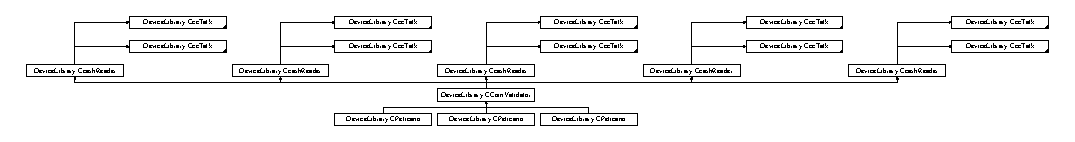
\includegraphics[height=1.465969cm]{class_device_library_1_1_c_coin_validator}
\end{center}
\end{figure}
\subsection*{Classes}
\begin{DoxyCompactItemize}
\item 
class \mbox{\hyperlink{class_device_library_1_1_c_coin_validator_1_1_c_c_vcredit_buffer}{C\+C\+Vcredit\+Buffer}}
\begin{DoxyCompactList}\small\item\em Classe du buffer des credits ou des codes erreurs. \end{DoxyCompactList}\item 
class \mbox{\hyperlink{class_device_library_1_1_c_coin_validator_1_1_c_erro_c_v}{C\+Erro\+CV}}
\end{DoxyCompactItemize}
\subsection*{Public Types}
\begin{DoxyCompactItemize}
\item 
enum \mbox{\hyperlink{class_device_library_1_1_c_coin_validator_a33c79ff59c961c2e1bbf95838e5d6871}{Etat}} \+: byte \{ \newline
\mbox{\hyperlink{class_device_library_1_1_c_coin_validator_a33c79ff59c961c2e1bbf95838e5d6871abb47b9b1d888741b1d94f3f060281299}{Etat.\+S\+T\+A\+T\+E\+\_\+\+I\+N\+IT}}, 
\mbox{\hyperlink{class_device_library_1_1_c_coin_validator_a33c79ff59c961c2e1bbf95838e5d6871aac8722b851146a23c4e0a59d1bd4b99d}{Etat.\+S\+T\+A\+T\+E\+\_\+\+R\+E\+S\+ET}}, 
\mbox{\hyperlink{class_device_library_1_1_c_coin_validator_a33c79ff59c961c2e1bbf95838e5d6871a0e7f32f0542fad5503628ce6a034fbd0}{Etat.\+S\+T\+A\+T\+E\+\_\+\+S\+I\+M\+P\+L\+E\+P\+O\+LL}}, 
\mbox{\hyperlink{class_device_library_1_1_c_coin_validator_a33c79ff59c961c2e1bbf95838e5d6871a403baa165578fb13762030b68713daca}{Etat.\+S\+T\+A\+T\+E\+\_\+\+G\+E\+T\+P\+O\+L\+L\+I\+N\+G\+P\+R\+I\+O\+R\+I\+TY}}, 
\newline
\mbox{\hyperlink{class_device_library_1_1_c_coin_validator_a33c79ff59c961c2e1bbf95838e5d6871ae5a739c65ca46caf6d8d388f3ae3f215}{Etat.\+S\+T\+A\+T\+E\+\_\+\+S\+E\+T\+P\+O\+L\+L\+I\+N\+G\+D\+E\+L\+AY}}, 
\mbox{\hyperlink{class_device_library_1_1_c_coin_validator_a33c79ff59c961c2e1bbf95838e5d6871a5fe7aa1c693d66ec83b4b57414702906}{Etat.\+S\+T\+A\+T\+E\+\_\+\+G\+E\+T\+S\+T\+A\+T\+US}}, 
\mbox{\hyperlink{class_device_library_1_1_c_coin_validator_a33c79ff59c961c2e1bbf95838e5d6871a1ef6b5f52c14078101e5e3667d47737b}{Etat.\+S\+T\+A\+T\+E\+\_\+\+G\+E\+T\+M\+A\+N\+U\+F\+A\+C\+T\+U\+R\+E\+R\+ID}}, 
\mbox{\hyperlink{class_device_library_1_1_c_coin_validator_a33c79ff59c961c2e1bbf95838e5d6871a8a6438b30205094505f9334a05dfb181}{Etat.\+S\+T\+A\+T\+E\+\_\+\+G\+E\+T\+E\+Q\+U\+I\+P\+E\+M\+E\+N\+T\+C\+A\+T\+E\+G\+O\+RY}}, 
\newline
\mbox{\hyperlink{class_device_library_1_1_c_coin_validator_a33c79ff59c961c2e1bbf95838e5d6871a265206139b5c776e496bbe0560ccfc99}{Etat.\+S\+T\+A\+T\+E\+\_\+\+G\+E\+T\+P\+R\+O\+D\+U\+C\+T\+C\+O\+DE}}, 
\mbox{\hyperlink{class_device_library_1_1_c_coin_validator_a33c79ff59c961c2e1bbf95838e5d6871a4a67b9a79581b431503084482a07723f}{Etat.\+S\+T\+A\+T\+E\+\_\+\+G\+E\+T\+B\+U\+I\+L\+D\+C\+O\+DE}}, 
\mbox{\hyperlink{class_device_library_1_1_c_coin_validator_a33c79ff59c961c2e1bbf95838e5d6871aa8ecbe1a24b3fa5a9b22c7c3d5af26f2}{Etat.\+S\+T\+A\+T\+E\+\_\+\+G\+E\+T\+D\+A\+T\+A\+B\+A\+S\+E\+V\+E\+R\+S\+I\+ON}}, 
\mbox{\hyperlink{class_device_library_1_1_c_coin_validator_a33c79ff59c961c2e1bbf95838e5d6871a247eb9a3665774bf7214dd78c11416e7}{Etat.\+S\+T\+A\+T\+E\+\_\+\+G\+E\+T\+S\+E\+R\+I\+A\+L\+N\+U\+M\+B\+ER}}, 
\newline
\mbox{\hyperlink{class_device_library_1_1_c_coin_validator_a33c79ff59c961c2e1bbf95838e5d6871a76b19450787b4b3caffafa35d8216920}{Etat.\+S\+T\+A\+T\+E\+\_\+\+G\+E\+T\+S\+O\+F\+T\+W\+A\+R\+E\+R\+E\+V\+I\+S\+I\+ON}}, 
\mbox{\hyperlink{class_device_library_1_1_c_coin_validator_a33c79ff59c961c2e1bbf95838e5d6871a705114ed45d23f5474f073c83ed34198}{Etat.\+S\+T\+A\+T\+E\+\_\+\+T\+E\+S\+T\+S\+O\+L\+E\+N\+O\+ID}}, 
\mbox{\hyperlink{class_device_library_1_1_c_coin_validator_a33c79ff59c961c2e1bbf95838e5d6871af24075f047ffa05c28715458f60f6c2e}{Etat.\+S\+T\+A\+T\+E\+\_\+\+T\+R\+A\+S\+H\+E\+M\+P\+TY}}, 
\mbox{\hyperlink{class_device_library_1_1_c_coin_validator_a33c79ff59c961c2e1bbf95838e5d6871a842db363f372d4400c74da269105c6f1}{Etat.\+S\+T\+A\+T\+E\+\_\+\+S\+E\+T\+S\+P\+E\+E\+D\+M\+O\+T\+OR}}, 
\newline
\mbox{\hyperlink{class_device_library_1_1_c_coin_validator_a33c79ff59c961c2e1bbf95838e5d6871aab26c5005c0ee5838edc28975e09a61a}{Etat.\+S\+T\+A\+T\+E\+\_\+\+G\+E\+T\+S\+P\+E\+E\+D\+M\+O\+T\+OR}}, 
\mbox{\hyperlink{class_device_library_1_1_c_coin_validator_a33c79ff59c961c2e1bbf95838e5d6871a4714312431af83bc3474f314b18fae80}{Etat.\+S\+T\+A\+T\+E\+\_\+\+G\+E\+T\+P\+O\+C\+K\+ET}}, 
\mbox{\hyperlink{class_device_library_1_1_c_coin_validator_a33c79ff59c961c2e1bbf95838e5d6871a869a56a581e853e5d15226930e13ff5d}{Etat.\+S\+T\+A\+T\+E\+\_\+\+C\+H\+E\+C\+K\+T\+R\+A\+S\+H\+D\+O\+OR}}, 
\mbox{\hyperlink{class_device_library_1_1_c_coin_validator_a33c79ff59c961c2e1bbf95838e5d6871a3a9f94ad405119ae73f2c6410d1cd9f2}{Etat.\+S\+T\+A\+T\+E\+\_\+\+C\+H\+E\+C\+K\+L\+O\+W\+E\+R\+S\+E\+N\+S\+OR}}, 
\newline
\mbox{\hyperlink{class_device_library_1_1_c_coin_validator_a33c79ff59c961c2e1bbf95838e5d6871afb0753c5cac9583b20e52e08e97b44d6}{Etat.\+S\+T\+A\+T\+E\+\_\+\+S\+E\+L\+F\+\_\+\+T\+E\+ST}}, 
\mbox{\hyperlink{class_device_library_1_1_c_coin_validator_a33c79ff59c961c2e1bbf95838e5d6871a73daf91486dd909820faca0e91882beb}{Etat.\+S\+T\+A\+T\+E\+\_\+\+S\+E\+T\+I\+N\+H\+I\+B\+I\+T\+S\+T\+A\+T\+US}}, 
\mbox{\hyperlink{class_device_library_1_1_c_coin_validator_a33c79ff59c961c2e1bbf95838e5d6871a50fe44dca28a30766a5649bf8b9afe9e}{Etat.\+S\+T\+A\+T\+E\+\_\+\+G\+E\+T\+I\+N\+H\+I\+B\+I\+T\+S\+T\+A\+T\+US}}, 
\mbox{\hyperlink{class_device_library_1_1_c_coin_validator_a33c79ff59c961c2e1bbf95838e5d6871affadcf3cb0d39b38a8f3ca88f7388901}{Etat.\+S\+T\+A\+T\+E\+\_\+\+G\+E\+T\+C\+R\+E\+D\+I\+T\+B\+U\+F\+F\+ER}}, 
\newline
\mbox{\hyperlink{class_device_library_1_1_c_coin_validator_a33c79ff59c961c2e1bbf95838e5d6871a9c1c69e1319855b5d761830ce685c96a}{Etat.\+S\+T\+A\+T\+E\+\_\+\+S\+E\+T\+M\+A\+S\+T\+E\+R\+I\+N\+H\+I\+B\+IT}}, 
\mbox{\hyperlink{class_device_library_1_1_c_coin_validator_a33c79ff59c961c2e1bbf95838e5d6871afc72fc11a904ff5f61cec6c9c34f2115}{Etat.\+S\+T\+A\+T\+E\+\_\+\+D\+I\+S\+A\+B\+L\+E\+M\+A\+S\+T\+ER}}, 
\mbox{\hyperlink{class_device_library_1_1_c_coin_validator_a33c79ff59c961c2e1bbf95838e5d6871a12de40f0f8ff40b07c2ebc106d6626dc}{Etat.\+S\+T\+A\+T\+E\+\_\+\+E\+N\+A\+B\+L\+E\+M\+A\+S\+T\+ER}}, 
\mbox{\hyperlink{class_device_library_1_1_c_coin_validator_a33c79ff59c961c2e1bbf95838e5d6871a16a0d4edbb28a34848d155e347f50d07}{Etat.\+S\+T\+A\+T\+E\+\_\+\+G\+E\+T\+M\+A\+S\+T\+E\+R\+I\+N\+H\+I\+BT}}, 
\newline
\mbox{\hyperlink{class_device_library_1_1_c_coin_validator_a33c79ff59c961c2e1bbf95838e5d6871abd893617ba11bba9f46a4e7dde1e14ba}{Etat.\+S\+T\+A\+T\+E\+\_\+\+S\+E\+T\+O\+V\+E\+R\+R\+I\+DE}}, 
\mbox{\hyperlink{class_device_library_1_1_c_coin_validator_a33c79ff59c961c2e1bbf95838e5d6871a549141cb843ccc9e63a5a27d689e4f8a}{Etat.\+S\+T\+A\+T\+E\+\_\+\+G\+E\+T\+O\+V\+E\+R\+R\+I\+DE}}, 
\mbox{\hyperlink{class_device_library_1_1_c_coin_validator_a33c79ff59c961c2e1bbf95838e5d6871a119e95d1b7ccb2fe9684fab70ff434a4}{Etat.\+S\+T\+A\+T\+E\+\_\+\+G\+E\+T\+O\+P\+T\+I\+ON}}, 
\mbox{\hyperlink{class_device_library_1_1_c_coin_validator_a33c79ff59c961c2e1bbf95838e5d6871aebb524d9d2939864e4b98146fa2eda6f}{Etat.\+S\+T\+A\+T\+E\+\_\+\+S\+E\+T\+S\+O\+R\+T\+E\+R\+P\+A\+TH}}, 
\newline
\mbox{\hyperlink{class_device_library_1_1_c_coin_validator_a33c79ff59c961c2e1bbf95838e5d6871aa9682c56a455bd2f1a9f57e32e7639fc}{Etat.\+S\+T\+A\+T\+E\+\_\+\+G\+E\+T\+S\+O\+R\+T\+E\+R\+P\+A\+TH}}, 
\mbox{\hyperlink{class_device_library_1_1_c_coin_validator_a33c79ff59c961c2e1bbf95838e5d6871aa3c6eabffd1821f7c63dc12015ca8fb1}{Etat.\+S\+T\+A\+T\+E\+\_\+\+S\+E\+T\+D\+E\+F\+A\+U\+L\+T\+S\+O\+R\+T\+E\+R\+P\+A\+TH}}, 
\mbox{\hyperlink{class_device_library_1_1_c_coin_validator_a33c79ff59c961c2e1bbf95838e5d6871a59085e963dfd65a5fbe264fccc6c6d2e}{Etat.\+S\+T\+A\+T\+E\+\_\+\+G\+E\+T\+D\+E\+F\+A\+U\+L\+T\+S\+O\+R\+T\+E\+R\+P\+A\+TH}}, 
\mbox{\hyperlink{class_device_library_1_1_c_coin_validator_a33c79ff59c961c2e1bbf95838e5d6871a3b1dbe60c4b27db6a2570d8267c81a93}{Etat.\+S\+T\+A\+T\+E\+\_\+\+G\+E\+T\+C\+O\+I\+N\+ID}}, 
\newline
\mbox{\hyperlink{class_device_library_1_1_c_coin_validator_a33c79ff59c961c2e1bbf95838e5d6871ae7d6e6ee885540e3f876a92a7e57b96c}{Etat.\+S\+T\+A\+T\+E\+\_\+\+A\+C\+C\+E\+P\+T\+L\+I\+M\+IT}}, 
\mbox{\hyperlink{class_device_library_1_1_c_coin_validator_a33c79ff59c961c2e1bbf95838e5d6871af4dadaba24e538c246b8c3dd3833ab7e}{Etat.\+S\+T\+A\+T\+E\+\_\+\+C\+O\+M\+M\+S\+R\+E\+V\+I\+S\+I\+ON}}, 
\mbox{\hyperlink{class_device_library_1_1_c_coin_validator_a33c79ff59c961c2e1bbf95838e5d6871a3f4ffd4998d3212972d11f59c018692c}{Etat.\+S\+T\+A\+T\+E\+\_\+\+C\+H\+E\+C\+K\+C\+R\+E\+D\+I\+B\+U\+F\+F\+ER}}, 
\mbox{\hyperlink{class_device_library_1_1_c_coin_validator_a33c79ff59c961c2e1bbf95838e5d6871a667adf1721ecf31975b473ea51005d04}{Etat.\+S\+T\+A\+T\+E\+\_\+\+I\+D\+LE}} = 0\+X\+FF
 \}
\begin{DoxyCompactList}\small\item\em Etat de la machine d\textquotesingle{}état du CV. \end{DoxyCompactList}\item 
enum \mbox{\hyperlink{group___erreur_ga68c5b73cc3b337502d9f92154d933591}{C\+V\+Error\+Codes}} \+: byte \{ \newline
\mbox{\hyperlink{group___erreur_gga68c5b73cc3b337502d9f92154d933591a6c3e226b4d4795d518ab341b0824ec29}{C\+V\+Error\+Codes.\+N\+U\+LL}} = 0, 
\mbox{\hyperlink{group___erreur_gga68c5b73cc3b337502d9f92154d933591a4a3172fa5d33d5089aa41cf83c8099f8}{C\+V\+Error\+Codes.\+R\+E\+J\+E\+C\+T\+C\+O\+IN}} = 1, 
\mbox{\hyperlink{group___erreur_gga68c5b73cc3b337502d9f92154d933591a236caf0a304503bf0fca29ee75e1d863}{C\+V\+Error\+Codes.\+I\+N\+H\+I\+B\+I\+T\+E\+D\+C\+O\+IN}} = 2, 
\mbox{\hyperlink{group___erreur_gga68c5b73cc3b337502d9f92154d933591ae56f4cf37b6999372dc21bb47e82d73c}{C\+V\+Error\+Codes.\+M\+U\+L\+T\+I\+P\+L\+E\+W\+I\+N\+D\+O\+WS}} = 3, 
\newline
\mbox{\hyperlink{group___erreur_gga68c5b73cc3b337502d9f92154d933591a875eb06a96859ac39b2ff14d3a5360de}{C\+V\+Error\+Codes.\+W\+A\+K\+E\+U\+P\+\_\+\+TO}} = 4, 
\mbox{\hyperlink{group___erreur_gga68c5b73cc3b337502d9f92154d933591a1de1001e85495d060e5fe77182345937}{C\+V\+Error\+Codes.\+V\+A\+L\+I\+D\+A\+T\+I\+O\+N\+\_\+\+TO}} = 5, 
\mbox{\hyperlink{group___erreur_gga68c5b73cc3b337502d9f92154d933591ae8e1da986224d6127b836dee5515b989}{C\+V\+Error\+Codes.\+C\+R\+E\+D\+I\+T\+S\+E\+N\+S\+O\+R\+\_\+\+TO}} = 6, 
\mbox{\hyperlink{group___erreur_gga68c5b73cc3b337502d9f92154d933591aad786ab20e40eca4baf577f142271223}{C\+V\+Error\+Codes.\+S\+O\+R\+T\+E\+R\+O\+P\+T\+O\+\_\+\+TO}} = 7, 
\newline
\mbox{\hyperlink{group___erreur_gga68c5b73cc3b337502d9f92154d933591a67eeaa2b6e727735860ab0fa45da5cf6}{C\+V\+Error\+Codes.\+T\+O\+O\+C\+L\+O\+S\+E\+C\+O\+IN}} = 8, 
\mbox{\hyperlink{group___erreur_gga68c5b73cc3b337502d9f92154d933591a488417ec04b13c6dcf02bdecb8597051}{C\+V\+Error\+Codes.\+A\+C\+C\+E\+P\+T\+G\+A\+T\+E\+N\+O\+T\+R\+E\+A\+DY}} = 9, 
\mbox{\hyperlink{group___erreur_gga68c5b73cc3b337502d9f92154d933591aa5c66915ba05071d42f5262814f1f154}{C\+V\+Error\+Codes.\+C\+R\+E\+D\+I\+T\+S\+E\+N\+S\+O\+R\+N\+O\+T\+R\+E\+A\+DY}} = 10, 
\mbox{\hyperlink{group___erreur_gga68c5b73cc3b337502d9f92154d933591aeb24605f73e423b795d431b13e81789d}{C\+V\+Error\+Codes.\+S\+O\+R\+T\+E\+R\+N\+O\+T\+R\+E\+A\+DY}} = 11, 
\newline
\mbox{\hyperlink{group___erreur_gga68c5b73cc3b337502d9f92154d933591a5f05f23aa23d4394442a22d01092b185}{C\+V\+Error\+Codes.\+R\+E\+J\+E\+C\+T\+C\+O\+I\+N\+N\+O\+T\+C\+L\+E\+A\+R\+ED}} = 12, 
\mbox{\hyperlink{group___erreur_gga68c5b73cc3b337502d9f92154d933591a529f5ada9f1b5031cdb17562a57bf07c}{C\+V\+Error\+Codes.\+V\+A\+L\+I\+D\+A\+T\+O\+R\+S\+E\+N\+S\+O\+R\+N\+O\+T\+R\+E\+A\+DY}} = 13, 
\mbox{\hyperlink{group___erreur_gga68c5b73cc3b337502d9f92154d933591ad9dfefcc80c822a24a0ad3380eb36cf2}{C\+V\+Error\+Codes.\+C\+R\+E\+D\+I\+T\+S\+E\+N\+S\+O\+R\+B\+L\+O\+C\+K\+ED}} = 14, 
\mbox{\hyperlink{group___erreur_gga68c5b73cc3b337502d9f92154d933591ad5ffb15a2080554273173e94ab156096}{C\+V\+Error\+Codes.\+S\+O\+R\+T\+E\+R\+O\+P\+T\+O\+B\+L\+O\+C\+K\+ED}} = 15, 
\newline
\mbox{\hyperlink{group___erreur_gga68c5b73cc3b337502d9f92154d933591afd097e798482607f42e03a4fe28a4040}{C\+V\+Error\+Codes.\+C\+R\+E\+D\+I\+T\+S\+E\+Q\+E\+R\+R\+OR}} = 16, 
\mbox{\hyperlink{group___erreur_gga68c5b73cc3b337502d9f92154d933591ad092fef941ebaf843780f10dc910af1c}{C\+V\+Error\+Codes.\+C\+O\+I\+N\+G\+O\+I\+N\+G\+B\+A\+CK}} = 17, 
\mbox{\hyperlink{group___erreur_gga68c5b73cc3b337502d9f92154d933591a561dba7292ec10b3dd57fc75609c82d8}{C\+V\+Error\+Codes.\+C\+O\+I\+N\+T\+O\+O\+F\+A\+ST}} = 18, 
\mbox{\hyperlink{group___erreur_gga68c5b73cc3b337502d9f92154d933591a44c9d0c8f952ac7cd9976e8d9cb0b5ac}{C\+V\+Error\+Codes.\+C\+O\+I\+N\+T\+O\+O\+S\+L\+OW}} = 19, 
\newline
\mbox{\hyperlink{group___erreur_gga68c5b73cc3b337502d9f92154d933591a8fe88ac7acc89aaabdb1bd870fd7ceb2}{C\+V\+Error\+Codes.\+C\+O\+S\+M\+E\+C\+H\+A\+C\+T\+I\+V\+ED}} = 20, 
\mbox{\hyperlink{group___erreur_gga68c5b73cc3b337502d9f92154d933591abcdd757e0380f69f13dff8be4d7d247f}{C\+V\+Error\+Codes.\+D\+C\+E\+O\+P\+T\+O\+\_\+\+TO}} = 21, 
\mbox{\hyperlink{group___erreur_gga68c5b73cc3b337502d9f92154d933591a31c99e9aae78a22cd697c80f35779083}{C\+V\+Error\+Codes.\+D\+C\+E\+O\+P\+T\+O\+N\+O\+T\+S\+EE}} = 22, 
\mbox{\hyperlink{group___erreur_gga68c5b73cc3b337502d9f92154d933591a6fd6e43dc5f964d3b48ad0c245d9dc50}{C\+V\+Error\+Codes.\+C\+R\+E\+D\+I\+T\+S\+E\+N\+S\+O\+R\+R\+E\+A\+C\+H\+E\+D\+E\+A\+R\+LY}} = 23, 
\newline
\mbox{\hyperlink{group___erreur_gga68c5b73cc3b337502d9f92154d933591aed7cae4a3226e4da365e7c9c5a8d347f}{C\+V\+Error\+Codes.\+R\+E\+J\+E\+C\+T\+E\+D\+C\+O\+I\+N2}} = 24, 
\mbox{\hyperlink{group___erreur_gga68c5b73cc3b337502d9f92154d933591a21aa9d7cf65b4208ae81a40097ce9d26}{C\+V\+Error\+Codes.\+R\+E\+J\+E\+C\+T\+S\+L\+UG}} = 25, 
\mbox{\hyperlink{group___erreur_gga68c5b73cc3b337502d9f92154d933591a8823666fd9f278f2700a27f91799b65d}{C\+V\+Error\+Codes.\+R\+E\+J\+E\+C\+T\+S\+E\+N\+S\+O\+R\+B\+L\+O\+C\+K\+ED}} = 26, 
\mbox{\hyperlink{group___erreur_gga68c5b73cc3b337502d9f92154d933591acd4f575618900c07705e0f3ed6a72a16}{C\+V\+Error\+Codes.\+G\+A\+M\+E\+S\+O\+V\+E\+R\+L\+O\+AD}} = 27, 
\newline
\mbox{\hyperlink{group___erreur_gga68c5b73cc3b337502d9f92154d933591acb5a7731b62453102c5cd6211bc6a6f8}{C\+V\+Error\+Codes.\+M\+A\+X\+C\+O\+I\+N\+M\+E\+T\+E\+R\+P\+U\+L\+S\+E\+S\+E\+X\+C\+E\+E\+D\+ED}} = 28, 
\mbox{\hyperlink{group___erreur_gga68c5b73cc3b337502d9f92154d933591a713b07a2ec4a9014b2fdb72c5d8d8980}{C\+V\+Error\+Codes.\+A\+C\+C\+E\+P\+T\+G\+A\+T\+E\+O\+P\+E\+N\+N\+O\+T\+C\+L\+O\+S\+ED}} = 29, 
\mbox{\hyperlink{group___erreur_gga68c5b73cc3b337502d9f92154d933591ad697f2db067ec6160ac3c98dbd7acbc3}{C\+V\+Error\+Codes.\+A\+C\+C\+E\+P\+T\+G\+A\+T\+E\+C\+L\+O\+S\+E\+D\+N\+O\+T\+O\+P\+EN}} = 30, 
\mbox{\hyperlink{group___erreur_gga68c5b73cc3b337502d9f92154d933591a1f2e8ea805df9a9e6a9128576e2f342b}{C\+V\+Error\+Codes.\+M\+A\+N\+I\+F\+O\+L\+D\+T\+I\+M\+E\+O\+UT}} = 31, 
\newline
\mbox{\hyperlink{group___erreur_gga68c5b73cc3b337502d9f92154d933591a30272f8d3111e39e72b1bea11c4a2906}{C\+V\+Error\+Codes.\+M\+A\+N\+I\+F\+O\+L\+D\+O\+P\+T\+O\+B\+L\+O\+C\+K\+ED}} = 32, 
\mbox{\hyperlink{group___erreur_gga68c5b73cc3b337502d9f92154d933591a833a2d147bee60b116f24d87b3da8b82}{C\+V\+Error\+Codes.\+M\+A\+N\+I\+F\+O\+L\+D\+N\+O\+T\+R\+E\+A\+DY}} = 33, 
\mbox{\hyperlink{group___erreur_gga68c5b73cc3b337502d9f92154d933591a3a1f7e69b7e5e5c269e0fa7e97b0bf0a}{C\+V\+Error\+Codes.\+S\+E\+C\+U\+R\+I\+T\+Y\+S\+T\+A\+T\+U\+S\+C\+H\+A\+N\+G\+ED}} = 34, 
\mbox{\hyperlink{group___erreur_gga68c5b73cc3b337502d9f92154d933591a9f9cc74325b5bb6e924cd0772df6d6a6}{C\+V\+Error\+Codes.\+M\+O\+T\+O\+R\+E\+X\+C\+E\+P\+T\+I\+ON}} = 35, 
\newline
\mbox{\hyperlink{group___erreur_gga68c5b73cc3b337502d9f92154d933591ab04c310e6eb59f7ae1eb525e552bbe4f}{C\+V\+Error\+Codes.\+S\+W\+A\+L\+L\+O\+W\+E\+D\+C\+O\+IN}} = 36, 
\mbox{\hyperlink{group___erreur_gga68c5b73cc3b337502d9f92154d933591ada03008cb56819752dd1fe201c4c1be9}{C\+V\+Error\+Codes.\+C\+O\+I\+N2\+F\+A\+ST}} = 37, 
\mbox{\hyperlink{group___erreur_gga68c5b73cc3b337502d9f92154d933591ad4f375ed800d463da94afc540bf8d22e}{C\+V\+Error\+Codes.\+C\+O\+I\+N2\+S\+L\+OW}} = 38, 
\mbox{\hyperlink{group___erreur_gga68c5b73cc3b337502d9f92154d933591aa6c8fed14ab5411a4efe88068c4a99d9}{C\+V\+Error\+Codes.\+C\+O\+I\+N\+I\+N\+C\+O\+R\+R\+E\+C\+T\+L\+Y\+S\+O\+R\+T\+ED}} = 39, 
\newline
\mbox{\hyperlink{group___erreur_gga68c5b73cc3b337502d9f92154d933591afdbe0522298a7ecd540a24a4d368442a}{C\+V\+Error\+Codes.\+E\+X\+T\+E\+R\+N\+A\+L\+L\+I\+G\+H\+T\+A\+T\+T\+A\+CK}} = 40, 
\mbox{\hyperlink{group___erreur_gga68c5b73cc3b337502d9f92154d933591a69b954ad6ad0a788c70a17bc2f280d31}{C\+V\+Error\+Codes.\+I\+N\+H\+I\+B\+I\+T\+E\+D\+C\+O\+I\+N\+\_\+1}} = 128, 
\mbox{\hyperlink{group___erreur_gga68c5b73cc3b337502d9f92154d933591a07d7f9cdabc4510272dfc11e1bdbf3b7}{C\+V\+Error\+Codes.\+I\+N\+H\+I\+B\+I\+T\+E\+D\+C\+O\+I\+N\+\_\+2}} = 129, 
\mbox{\hyperlink{group___erreur_gga68c5b73cc3b337502d9f92154d933591a0c8fb65b7cf54e6352781e7869fd5b2e}{C\+V\+Error\+Codes.\+I\+N\+H\+I\+B\+I\+T\+E\+D\+C\+O\+I\+N\+\_\+3}} = 130, 
\newline
\mbox{\hyperlink{group___erreur_gga68c5b73cc3b337502d9f92154d933591a9931e14f9728388be7cea22a76d96df9}{C\+V\+Error\+Codes.\+I\+N\+H\+I\+B\+I\+T\+E\+D\+C\+O\+I\+N\+\_\+4}} = 131, 
\mbox{\hyperlink{group___erreur_gga68c5b73cc3b337502d9f92154d933591a583bc6ef29caaddcc110fb91d70869e2}{C\+V\+Error\+Codes.\+I\+N\+H\+I\+B\+I\+T\+E\+D\+C\+O\+I\+N\+\_\+5}} = 132, 
\mbox{\hyperlink{group___erreur_gga68c5b73cc3b337502d9f92154d933591ab9f53cc85987fb6065b91f00ab23b0bb}{C\+V\+Error\+Codes.\+I\+N\+H\+I\+B\+I\+T\+E\+D\+C\+O\+I\+N\+\_\+6}} = 133, 
\mbox{\hyperlink{group___erreur_gga68c5b73cc3b337502d9f92154d933591a8af6d4f0fcb2fb94e876a61fb37d727b}{C\+V\+Error\+Codes.\+I\+N\+H\+I\+B\+I\+T\+E\+D\+C\+O\+I\+N\+\_\+7}} = 134, 
\newline
\mbox{\hyperlink{group___erreur_gga68c5b73cc3b337502d9f92154d933591a3cf9f08f6eae082afd768c3a97e841c8}{C\+V\+Error\+Codes.\+I\+N\+H\+I\+B\+I\+T\+E\+D\+C\+O\+I\+N\+\_\+8}} = 135, 
\mbox{\hyperlink{group___erreur_gga68c5b73cc3b337502d9f92154d933591aab7979ee88a0c918182eb43826f2ebee}{C\+V\+Error\+Codes.\+I\+N\+H\+I\+B\+I\+T\+E\+D\+C\+O\+I\+N\+\_\+9}} = 136, 
\mbox{\hyperlink{group___erreur_gga68c5b73cc3b337502d9f92154d933591ac609cf3e7418d787d165294c64e7f7f2}{C\+V\+Error\+Codes.\+I\+N\+H\+I\+B\+I\+T\+E\+D\+C\+O\+I\+N\+\_\+10}} = 137, 
\mbox{\hyperlink{group___erreur_gga68c5b73cc3b337502d9f92154d933591a5b0f85525816fde9150d1954f0f6a7c4}{C\+V\+Error\+Codes.\+I\+N\+H\+I\+B\+I\+T\+E\+D\+C\+O\+I\+N\+\_\+11}} = 138, 
\newline
\mbox{\hyperlink{group___erreur_gga68c5b73cc3b337502d9f92154d933591a587f525dad0c2d05cb8b00d0e2ea41ca}{C\+V\+Error\+Codes.\+I\+N\+H\+I\+B\+I\+T\+E\+D\+C\+O\+I\+N\+\_\+12}} = 139, 
\mbox{\hyperlink{group___erreur_gga68c5b73cc3b337502d9f92154d933591a2eacff30716ef2759d575926dc60fc85}{C\+V\+Error\+Codes.\+I\+N\+H\+I\+B\+I\+T\+E\+D\+C\+O\+I\+N\+\_\+13}} = 140, 
\mbox{\hyperlink{group___erreur_gga68c5b73cc3b337502d9f92154d933591a15a3c52c2473d645b8af3e70e3c3941e}{C\+V\+Error\+Codes.\+I\+N\+H\+I\+B\+I\+T\+E\+D\+C\+O\+I\+N\+\_\+14}} = 141, 
\mbox{\hyperlink{group___erreur_gga68c5b73cc3b337502d9f92154d933591a09c9109be00bc6033478fde72cd77403}{C\+V\+Error\+Codes.\+I\+N\+H\+I\+B\+I\+T\+E\+D\+C\+O\+I\+N\+\_\+15}} = 142, 
\newline
\mbox{\hyperlink{group___erreur_gga68c5b73cc3b337502d9f92154d933591a943bd83bbd39776c12e6e50a34bafb20}{C\+V\+Error\+Codes.\+I\+N\+H\+I\+B\+I\+T\+E\+D\+C\+O\+I\+N\+\_\+16}} = 143, 
\mbox{\hyperlink{group___erreur_gga68c5b73cc3b337502d9f92154d933591a78ad72ba807b0a50814dd29b3d7ea6bc}{C\+V\+Error\+Codes.\+I\+N\+H\+I\+B\+I\+T\+E\+D\+C\+O\+I\+N\+\_\+17}} = 144, 
\mbox{\hyperlink{group___erreur_gga68c5b73cc3b337502d9f92154d933591ad7108d43a2cb300a36f3cdc179eb6a47}{C\+V\+Error\+Codes.\+I\+N\+H\+I\+B\+I\+T\+E\+D\+C\+O\+I\+N\+\_\+18}} = 145, 
\mbox{\hyperlink{group___erreur_gga68c5b73cc3b337502d9f92154d933591afa829333e824a07d4a8ebcca5e1a51cb}{C\+V\+Error\+Codes.\+I\+N\+H\+I\+B\+I\+T\+E\+D\+C\+O\+I\+N\+\_\+19}} = 146, 
\newline
\mbox{\hyperlink{group___erreur_gga68c5b73cc3b337502d9f92154d933591a5f2a72bd8d3110eb145e95b2da42a9c9}{C\+V\+Error\+Codes.\+I\+N\+H\+I\+B\+I\+T\+E\+D\+C\+O\+I\+N\+\_\+20}} = 147, 
\mbox{\hyperlink{group___erreur_gga68c5b73cc3b337502d9f92154d933591a8447ec5ec7ae09fb62e8c9fae3dcb03f}{C\+V\+Error\+Codes.\+I\+N\+H\+I\+B\+I\+T\+E\+D\+C\+O\+I\+N\+\_\+21}} = 148, 
\mbox{\hyperlink{group___erreur_gga68c5b73cc3b337502d9f92154d933591a120f40242976f7da2c4375de7e738ae1}{C\+V\+Error\+Codes.\+I\+N\+H\+I\+B\+I\+T\+E\+D\+C\+O\+I\+N\+\_\+22}} = 149, 
\mbox{\hyperlink{group___erreur_gga68c5b73cc3b337502d9f92154d933591a3e9edbe8264331eee676a0f9e5f40e01}{C\+V\+Error\+Codes.\+I\+N\+H\+I\+B\+I\+T\+E\+D\+C\+O\+I\+N\+\_\+23}} = 150, 
\newline
\mbox{\hyperlink{group___erreur_gga68c5b73cc3b337502d9f92154d933591a1bcc40b7e814ef95f0781079a0fed830}{C\+V\+Error\+Codes.\+I\+N\+H\+I\+B\+I\+T\+E\+D\+C\+O\+I\+N\+\_\+24}} = 151, 
\mbox{\hyperlink{group___erreur_gga68c5b73cc3b337502d9f92154d933591a83da0b1354428b08469d611ebd7cc209}{C\+V\+Error\+Codes.\+I\+N\+H\+I\+B\+I\+T\+E\+D\+C\+O\+I\+N\+\_\+25}} = 152, 
\mbox{\hyperlink{group___erreur_gga68c5b73cc3b337502d9f92154d933591a2ee2098b225ed3267340fcb4cf8bef7f}{C\+V\+Error\+Codes.\+I\+N\+H\+I\+B\+I\+T\+E\+D\+C\+O\+I\+N\+\_\+26}} = 153, 
\mbox{\hyperlink{group___erreur_gga68c5b73cc3b337502d9f92154d933591afd42c8c1e81adbaae30e5d950d87fc91}{C\+V\+Error\+Codes.\+I\+N\+H\+I\+B\+I\+T\+E\+D\+C\+O\+I\+N\+\_\+27}} = 154, 
\newline
\mbox{\hyperlink{group___erreur_gga68c5b73cc3b337502d9f92154d933591a92bbc06e80c7891c058dd4f82f21cc84}{C\+V\+Error\+Codes.\+I\+N\+H\+I\+B\+I\+T\+E\+D\+C\+O\+I\+N\+\_\+28}} = 155, 
\mbox{\hyperlink{group___erreur_gga68c5b73cc3b337502d9f92154d933591a847a981b702782737c4d8d68ae43df96}{C\+V\+Error\+Codes.\+I\+N\+H\+I\+B\+I\+T\+E\+D\+C\+O\+I\+N\+\_\+29}} = 156, 
\mbox{\hyperlink{group___erreur_gga68c5b73cc3b337502d9f92154d933591a9eacc103c55f026c6d4c55d9145dc46c}{C\+V\+Error\+Codes.\+I\+N\+H\+I\+B\+I\+T\+E\+D\+C\+O\+I\+N\+\_\+30}} = 157, 
\mbox{\hyperlink{group___erreur_gga68c5b73cc3b337502d9f92154d933591a7650c785d588d5d802dc392398b5731a}{C\+V\+Error\+Codes.\+I\+N\+H\+I\+B\+I\+T\+E\+D\+C\+O\+I\+N\+\_\+31}} = 158, 
\newline
\mbox{\hyperlink{group___erreur_gga68c5b73cc3b337502d9f92154d933591a0e534ed5f2068211f3b791d94aada1e2}{C\+V\+Error\+Codes.\+I\+N\+H\+I\+B\+I\+T\+E\+D\+C\+O\+I\+N\+\_\+32}} = 159, 
\mbox{\hyperlink{group___erreur_gga68c5b73cc3b337502d9f92154d933591a05062f9114d515e6e34b9b781a68e042}{C\+V\+Error\+Codes.\+D\+A\+T\+A\+B\+L\+O\+C\+K\+R\+E\+Q\+U\+E\+S\+T\+ED}} = 253, 
\mbox{\hyperlink{group___erreur_gga68c5b73cc3b337502d9f92154d933591aa0d2119ea2041bc3e038f9f5f6f5f7b1}{C\+V\+Error\+Codes.\+C\+O\+I\+N\+R\+E\+T\+U\+R\+N\+M\+E\+C\+H\+A\+C\+T\+I\+V\+A\+T\+ED}} = 254, 
\mbox{\hyperlink{group___erreur_gga68c5b73cc3b337502d9f92154d933591a9993b5434242a3193a7a92cfe80b28ab}{C\+V\+Error\+Codes.\+U\+N\+S\+P\+E\+C\+I\+F\+I\+E\+D\+A\+L\+A\+RM}} = 255
 \}
\begin{DoxyCompactList}\small\item\em Enumération des codes erreur du monnayeur \end{DoxyCompactList}\end{DoxyCompactItemize}
\subsection*{Public Member Functions}
\begin{DoxyCompactItemize}
\item 
\mbox{\hyperlink{class_device_library_1_1_c_coin_validator_addb8e79d5a3377a2aadef60fc1b19a53}{C\+Coin\+Validator}} ()
\begin{DoxyCompactList}\small\item\em Constructeur de la class \mbox{\hyperlink{class_device_library_1_1_c_coin_validator}{C\+Coin\+Validator}} \end{DoxyCompactList}\item 
void \mbox{\hyperlink{class_device_library_1_1_c_coin_validator_a274bb7c7d9bfe3d07beff3e3f3553de8}{Init}} ()
\begin{DoxyCompactList}\small\item\em Initialisation du monnayeur. \end{DoxyCompactList}\item 
override void \mbox{\hyperlink{class_device_library_1_1_c_coin_validator_a0e406f9e175eb8d295fe7406e6a948af}{Task\+Check\+Event\+CV}} ()
\begin{DoxyCompactList}\small\item\em Tâche de la machine d\textquotesingle{}état du monnayeur. \end{DoxyCompactList}\end{DoxyCompactItemize}
\subsection*{Public Attributes}
\begin{DoxyCompactItemize}
\item 
\mbox{\hyperlink{class_device_library_1_1_c_coin_validator_1_1_c_erro_c_v}{C\+Erro\+CV}} \mbox{\hyperlink{class_device_library_1_1_c_coin_validator_a03b7719015059d51c015f7a95f3b9cca}{error\+CV}}
\item 
const byte \mbox{\hyperlink{class_device_library_1_1_c_coin_validator_a68f118167bcdf23f194ef02b779d4333}{num\+Channel}} = 16
\begin{DoxyCompactList}\small\item\em Nombre de canaux du monnayeur. \end{DoxyCompactList}\item 
\mbox{\hyperlink{class_device_library_1_1_c_coin_validator_1_1_c_c_vcredit_buffer}{C\+C\+Vcredit\+Buffer}} \mbox{\hyperlink{class_device_library_1_1_c_coin_validator_a0fce3a5cb9d620de02a2d6bfd89d72b1}{credit\+Buffer}}
\begin{DoxyCompactList}\small\item\em Buffer contenant les informations sur les pièces lues ou les erreurs rencontrées \end{DoxyCompactList}\item 
\mbox{\hyperlink{class_device_library_1_1_c_canal}{C\+Canal}} \mbox{[}$\,$\mbox{]} \mbox{\hyperlink{class_device_library_1_1_c_coin_validator_afdeb88b9e7e981afd51bd1322e9f89e9}{canaux}}
\begin{DoxyCompactList}\small\item\em Tableau des canaux \end{DoxyCompactList}\item 
Thread \mbox{\hyperlink{class_device_library_1_1_c_coin_validator_ada11d6936d839ad456e2bd9e66f3eb31}{C\+V\+Task}}
\begin{DoxyCompactList}\small\item\em Thread de gestion de la machine d\textquotesingle{}état du monnayeur. \end{DoxyCompactList}\item 
byte \mbox{\hyperlink{class_device_library_1_1_c_coin_validator_ab293634863b100aad9f167f189b49f19}{sorter\+Path}}
\begin{DoxyCompactList}\small\item\em Chemin utilisé dans le trieur pour le canal \end{DoxyCompactList}\end{DoxyCompactItemize}
\subsection*{Protected Types}
\begin{DoxyCompactItemize}
\item 
enum \mbox{\hyperlink{class_device_library_1_1_c_coin_validator_a62ce7ca9d0cc8ef92edb58f06a34add1}{C\+V\+Status}} \{ \mbox{\hyperlink{class_device_library_1_1_c_coin_validator_a62ce7ca9d0cc8ef92edb58f06a34add1ae0aa021e21dddbd6d8cecec71e9cf564}{C\+V\+Status.\+OK}} = 0, 
\mbox{\hyperlink{class_device_library_1_1_c_coin_validator_a62ce7ca9d0cc8ef92edb58f06a34add1a09784ba0e9f8a177ad98970e07381792}{C\+V\+Status.\+C\+O\+I\+N\+R\+E\+T\+U\+R\+N\+A\+C\+T\+I\+V\+A\+T\+ED}} = 1, 
\mbox{\hyperlink{class_device_library_1_1_c_coin_validator_a62ce7ca9d0cc8ef92edb58f06a34add1a00b18151c2f99ce38f6a179e84697b04}{C\+V\+Status.\+C\+O\+S\+A\+C\+T\+I\+V\+A\+T\+ED}} = 2
 \}
\item 
enum \mbox{\hyperlink{class_device_library_1_1_c_coin_validator_aec7d217f486dbce4458a64bc071fa19d}{Trash\+Door}} \{ \mbox{\hyperlink{class_device_library_1_1_c_coin_validator_aec7d217f486dbce4458a64bc071fa19da110ccf2f5d2ff4eda1fd1a494293467d}{Trash\+Door.\+C\+L\+O\+S\+ED}} = 0, 
\mbox{\hyperlink{class_device_library_1_1_c_coin_validator_aec7d217f486dbce4458a64bc071fa19daa38bd5138bf35514df41a1795ebbf5c3}{Trash\+Door.\+O\+P\+EN}} = 1
 \}
\begin{DoxyCompactList}\small\item\em Etats de la porte de rejet. \end{DoxyCompactList}\item 
enum \mbox{\hyperlink{class_device_library_1_1_c_coin_validator_ab4d515bda1d8e8679ed7dc4cc3f5c40c}{Lower\+Sensor}} \{ \mbox{\hyperlink{class_device_library_1_1_c_coin_validator_ab4d515bda1d8e8679ed7dc4cc3f5c40ca88c189a42c87aa49d667fc8ab76bc323}{Lower\+Sensor.\+F\+R\+EE}} = 0, 
\mbox{\hyperlink{class_device_library_1_1_c_coin_validator_ab4d515bda1d8e8679ed7dc4cc3f5c40ca802706a9238e2928077f97736854bad4}{Lower\+Sensor.\+B\+U\+SY}} = 1
 \}
\begin{DoxyCompactList}\small\item\em Etat des optos de sortie. \end{DoxyCompactList}\item 
enum \mbox{\hyperlink{group___header_ga5672baec375c16b1ec7bdb4b85cebaa9}{Header}} \+: byte \{ \newline
\mbox{\hyperlink{group___header_gga5672baec375c16b1ec7bdb4b85cebaa9a9ce2b30cbcbda60f1a4e9d2cd5526d20}{Header.\+R\+E\+Q\+U\+E\+S\+T\+S\+T\+A\+T\+US}} = 248, 
\mbox{\hyperlink{group___header_gga5672baec375c16b1ec7bdb4b85cebaa9a085cadf3ee4fec13527da4cbdb2f9e0c}{Header.\+R\+E\+Q\+U\+E\+S\+T\+D\+A\+T\+A\+B\+A\+S\+E\+V\+ER}} = 243, 
\mbox{\hyperlink{group___header_gga5672baec375c16b1ec7bdb4b85cebaa9add5d1a1bac3f18225ae7c4dd94fbbec1}{Header.\+T\+E\+S\+T\+S\+O\+L\+E\+N\+O\+ID}} = 240, 
\mbox{\hyperlink{group___header_gga5672baec375c16b1ec7bdb4b85cebaa9a684e258f63334d457d2d4c2502820a6e}{Header.\+T\+E\+S\+T\+O\+U\+T\+P\+U\+T\+L\+I\+N\+ES}} = 238, 
\newline
\mbox{\hyperlink{group___header_gga5672baec375c16b1ec7bdb4b85cebaa9aa5e7b8fd4be5bf778c447908e8d8008e}{Header.\+R\+E\+A\+D\+I\+N\+P\+U\+T\+L\+I\+N\+ES}} = 237, 
\mbox{\hyperlink{group___header_gga5672baec375c16b1ec7bdb4b85cebaa9af7401a2b001f90c26bb2be51b83799b3}{Header.\+R\+E\+A\+D\+O\+P\+T\+O\+S\+T\+A\+T\+ES}} = 236, 
\mbox{\hyperlink{group___header_gga5672baec375c16b1ec7bdb4b85cebaa9a492365d426f17a41c4cbd8a9c4846bf9}{Header.\+R\+E\+A\+D\+B\+U\+F\+F\+E\+R\+C\+R\+E\+D\+IT}} = 229, 
\mbox{\hyperlink{group___header_gga5672baec375c16b1ec7bdb4b85cebaa9ac95be1f63c78dc1b65f01227ec227359}{Header.\+M\+O\+D\+I\+F\+Y\+O\+V\+E\+R\+R\+I\+D\+E\+S\+T\+A\+T\+US}} = 222, 
\newline
\mbox{\hyperlink{group___header_gga5672baec375c16b1ec7bdb4b85cebaa9adbe07970434b8affd947c208a125a2ec}{Header.\+R\+E\+Q\+U\+E\+S\+T\+O\+V\+E\+R\+R\+I\+D\+E\+S\+T\+A\+T\+US}} = 221, 
\mbox{\hyperlink{group___header_gga5672baec375c16b1ec7bdb4b85cebaa9a33964bfc1d0f61c0365163eb22258215}{Header.\+R\+E\+Q\+U\+E\+S\+T\+O\+P\+T\+I\+O\+N\+F\+L\+AG}} = 213, 
\mbox{\hyperlink{group___header_gga5672baec375c16b1ec7bdb4b85cebaa9ad756e6025d036867d08303eb2f842430}{Header.\+M\+O\+D\+I\+F\+Y\+S\+O\+R\+T\+E\+R\+P\+A\+TH}} = 210, 
\mbox{\hyperlink{group___header_gga5672baec375c16b1ec7bdb4b85cebaa9ada6d464dd6ed1209fdad7db02f4d644c}{Header.\+M\+O\+D\+I\+F\+Y\+D\+E\+F\+A\+U\+L\+T\+S\+O\+R\+T\+E\+R\+P\+A\+TH}} = 189, 
\newline
\mbox{\hyperlink{group___header_gga5672baec375c16b1ec7bdb4b85cebaa9ad5e22c5779cc7122c156c913d6602b6a}{Header.\+R\+E\+Q\+U\+E\+S\+T\+D\+E\+F\+A\+U\+L\+T\+S\+O\+R\+T\+E\+R\+P\+A\+TH}} = 188, 
\mbox{\hyperlink{group___header_gga5672baec375c16b1ec7bdb4b85cebaa9ab6f00a60b1b3cb6b3d3bbe852a099ecc}{Header.\+S\+E\+T\+A\+C\+C\+E\+P\+T\+L\+I\+M\+IT}} = 135
 \}
\begin{DoxyCompactList}\small\item\em Liste des headers spécifiques au monnayeur \end{DoxyCompactList}\end{DoxyCompactItemize}
\subsection*{Protected Member Functions}
\begin{DoxyCompactItemize}
\item 
bool \mbox{\hyperlink{class_device_library_1_1_c_coin_validator_aca5a7f6d4805b9cd2df7b4d4fbdd0686}{Test\+Solenoid}} (byte mask=0\+X01)
\begin{DoxyCompactList}\small\item\em Active les activateurs du monnayeur \end{DoxyCompactList}\item 
void \mbox{\hyperlink{class_device_library_1_1_c_coin_validator_a941fe54c9299c2f3d78f865a3c7dc720}{Set\+Override\+Status}} (byte mask)
\begin{DoxyCompactList}\small\item\em Modifie l\textquotesingle{}override status. \end{DoxyCompactList}\item 
void \mbox{\hyperlink{class_device_library_1_1_c_coin_validator_ac3b462f2745990be15e78aef12ceb0ce}{Check\+Credit\+Buffer}} ()
\begin{DoxyCompactList}\small\item\em Cette fonction analyse le buffer des crédits et des codes erreurs \end{DoxyCompactList}\item 
virtual void \mbox{\hyperlink{class_device_library_1_1_c_coin_validator_ad5060d28baf7c2abedc788c6bcdcb02d}{Check\+State}} ()
\begin{DoxyCompactList}\small\item\em Machine d\textquotesingle{}état du monnayeur. \end{DoxyCompactList}\end{DoxyCompactItemize}
\subsection*{Properties}
\begin{DoxyCompactItemize}
\item 
byte \mbox{\hyperlink{class_device_library_1_1_c_coin_validator_a8547317bb187fe7e1fa247b64bc94ed1}{Back\+Event\+Counter}}\hspace{0.3cm}{\ttfamily  \mbox{[}get, set\mbox{]}}
\begin{DoxyCompactList}\small\item\em Sauvegarde du compteur d\textquotesingle{}événement. \end{DoxyCompactList}\item 
bool \mbox{\hyperlink{class_device_library_1_1_c_coin_validator_af41e76ebe686da650b5a12ab034309ec}{Is\+C\+V\+To\+Be\+Deactivated}}\hspace{0.3cm}{\ttfamily  \mbox{[}get, set\mbox{]}}
\begin{DoxyCompactList}\small\item\em Indique si le monnayeur doit être adtivé. \end{DoxyCompactList}\item 
bool \mbox{\hyperlink{class_device_library_1_1_c_coin_validator_a6fe7522091654bc85951ad9f234b7585}{Is\+C\+V\+To\+Be\+Activated}}\hspace{0.3cm}{\ttfamily  \mbox{[}get, set\mbox{]}}
\begin{DoxyCompactList}\small\item\em Indique si le monnayeur doit être adtivé. \end{DoxyCompactList}\item 
\mbox{\hyperlink{class_device_library_1_1_c_coin_validator_aec7d217f486dbce4458a64bc071fa19d}{Trash\+Door}} \mbox{\hyperlink{class_device_library_1_1_c_coin_validator_aec2db3e243a0eb073f5392c41ee0c354}{Trash\+Lid}}\hspace{0.3cm}{\ttfamily  \mbox{[}get, set\mbox{]}}
\begin{DoxyCompactList}\small\item\em Contient l\textquotesingle{}indicateur d\textquotesingle{}ouverture du containner. \end{DoxyCompactList}\item 
\mbox{\hyperlink{class_device_library_1_1_c_coin_validator_ab4d515bda1d8e8679ed7dc4cc3f5c40c}{Lower\+Sensor}} \mbox{\hyperlink{class_device_library_1_1_c_coin_validator_a394bb70d5bee7bb9abbe32e332a49071}{Exit\+Sensor}}\hspace{0.3cm}{\ttfamily  \mbox{[}get, set\mbox{]}}
\begin{DoxyCompactList}\small\item\em Indique si les optiques de sortie sont libre. \end{DoxyCompactList}\item 
byte \mbox{\hyperlink{class_device_library_1_1_c_coin_validator_a31cbd99fe83d5483df49f401350c8a45}{Channel\+In\+Progress}}\hspace{0.3cm}{\ttfamily  \mbox{[}get, set\mbox{]}}
\begin{DoxyCompactList}\small\item\em Numéro du canal en cours d\textquotesingle{}utilisation. \end{DoxyCompactList}\item 
byte \mbox{\hyperlink{class_device_library_1_1_c_coin_validator_a065e536f9d47a78ab3bbc5fd2990ada0}{Override\+Mask}}\hspace{0.3cm}{\ttfamily  \mbox{[}get, set\mbox{]}}
\begin{DoxyCompactList}\small\item\em Masque des chemins optionnels \end{DoxyCompactList}\item 
\mbox{\hyperlink{class_device_library_1_1_c_coin_validator_a33c79ff59c961c2e1bbf95838e5d6871}{Etat}} \mbox{\hyperlink{class_device_library_1_1_c_coin_validator_a38527f741c0cee761a37bff50bafbd20}{State}}\hspace{0.3cm}{\ttfamily  \mbox{[}get, set\mbox{]}}
\begin{DoxyCompactList}\small\item\em Etat de la machie d\textquotesingle{}état. \end{DoxyCompactList}\item 
byte \mbox{\hyperlink{class_device_library_1_1_c_coin_validator_a8e3e78f989d6549af291def41d6f2498}{Data\+Base\+Version}}\hspace{0.3cm}{\ttfamily  \mbox{[}get\mbox{]}}
\begin{DoxyCompactList}\small\item\em Renvoi la version de la data base. \end{DoxyCompactList}\item 
byte \mbox{\hyperlink{class_device_library_1_1_c_coin_validator_a6febc69e244b62d2527286c2483f5a66}{Override\+Status}}\hspace{0.3cm}{\ttfamily  \mbox{[}get\mbox{]}}
\begin{DoxyCompactList}\small\item\em Renvoie l\textquotesingle{}override status. \end{DoxyCompactList}\item 
\mbox{\hyperlink{class_device_library_1_1_c_coin_validator_a62ce7ca9d0cc8ef92edb58f06a34add1}{C\+V\+Status}} \mbox{\hyperlink{class_device_library_1_1_c_coin_validator_ac45ed64d9685ac636e48b00510c7654e}{Status}}\hspace{0.3cm}{\ttfamily  \mbox{[}get\mbox{]}}
\begin{DoxyCompactList}\small\item\em Renvoi le status du coin validator \end{DoxyCompactList}\item 
byte \mbox{[}$\,$\mbox{]} \mbox{\hyperlink{class_device_library_1_1_c_coin_validator_a538e6fc08186ba969f190503cdc828c2}{Variables\+Set}}\hspace{0.3cm}{\ttfamily  \mbox{[}get\mbox{]}}
\begin{DoxyCompactList}\small\item\em Les donnees variables du monnaayeur. \end{DoxyCompactList}\end{DoxyCompactItemize}
\subsection*{Additional Inherited Members}


\subsection{Detailed Description}
Class gérant le monnayeur. 



\subsection{Member Enumeration Documentation}
\mbox{\Hypertarget{class_device_library_1_1_c_coin_validator_a62ce7ca9d0cc8ef92edb58f06a34add1}\label{class_device_library_1_1_c_coin_validator_a62ce7ca9d0cc8ef92edb58f06a34add1}} 
\index{Device\+Library\+::\+C\+Coin\+Validator@{Device\+Library\+::\+C\+Coin\+Validator}!C\+V\+Status@{C\+V\+Status}}
\index{C\+V\+Status@{C\+V\+Status}!Device\+Library\+::\+C\+Coin\+Validator@{Device\+Library\+::\+C\+Coin\+Validator}}
\subsubsection{\texorpdfstring{C\+V\+Status}{CVStatus}}
{\footnotesize\ttfamily enum \mbox{\hyperlink{class_device_library_1_1_c_coin_validator_a62ce7ca9d0cc8ef92edb58f06a34add1}{Device\+Library.\+C\+Coin\+Validator.\+C\+V\+Status}}\hspace{0.3cm}{\ttfamily [strong]}, {\ttfamily [protected]}}





\begin{DoxyEnumFields}{Enumerator}
\raisebox{\heightof{T}}[0pt][0pt]{\index{OK@{OK}!Device\+Library\+::\+C\+Coin\+Validator@{Device\+Library\+::\+C\+Coin\+Validator}}\index{Device\+Library\+::\+C\+Coin\+Validator@{Device\+Library\+::\+C\+Coin\+Validator}!OK@{OK}}}\mbox{\Hypertarget{class_device_library_1_1_c_coin_validator_a62ce7ca9d0cc8ef92edb58f06a34add1ae0aa021e21dddbd6d8cecec71e9cf564}\label{class_device_library_1_1_c_coin_validator_a62ce7ca9d0cc8ef92edb58f06a34add1ae0aa021e21dddbd6d8cecec71e9cf564}} 
OK&\\
\hline

\raisebox{\heightof{T}}[0pt][0pt]{\index{C\+O\+I\+N\+R\+E\+T\+U\+R\+N\+A\+C\+T\+I\+V\+A\+T\+ED@{C\+O\+I\+N\+R\+E\+T\+U\+R\+N\+A\+C\+T\+I\+V\+A\+T\+ED}!Device\+Library\+::\+C\+Coin\+Validator@{Device\+Library\+::\+C\+Coin\+Validator}}\index{Device\+Library\+::\+C\+Coin\+Validator@{Device\+Library\+::\+C\+Coin\+Validator}!C\+O\+I\+N\+R\+E\+T\+U\+R\+N\+A\+C\+T\+I\+V\+A\+T\+ED@{C\+O\+I\+N\+R\+E\+T\+U\+R\+N\+A\+C\+T\+I\+V\+A\+T\+ED}}}\mbox{\Hypertarget{class_device_library_1_1_c_coin_validator_a62ce7ca9d0cc8ef92edb58f06a34add1a09784ba0e9f8a177ad98970e07381792}\label{class_device_library_1_1_c_coin_validator_a62ce7ca9d0cc8ef92edb58f06a34add1a09784ba0e9f8a177ad98970e07381792}} 
C\+O\+I\+N\+R\+E\+T\+U\+R\+N\+A\+C\+T\+I\+V\+A\+T\+ED&\\
\hline

\raisebox{\heightof{T}}[0pt][0pt]{\index{C\+O\+S\+A\+C\+T\+I\+V\+A\+T\+ED@{C\+O\+S\+A\+C\+T\+I\+V\+A\+T\+ED}!Device\+Library\+::\+C\+Coin\+Validator@{Device\+Library\+::\+C\+Coin\+Validator}}\index{Device\+Library\+::\+C\+Coin\+Validator@{Device\+Library\+::\+C\+Coin\+Validator}!C\+O\+S\+A\+C\+T\+I\+V\+A\+T\+ED@{C\+O\+S\+A\+C\+T\+I\+V\+A\+T\+ED}}}\mbox{\Hypertarget{class_device_library_1_1_c_coin_validator_a62ce7ca9d0cc8ef92edb58f06a34add1a00b18151c2f99ce38f6a179e84697b04}\label{class_device_library_1_1_c_coin_validator_a62ce7ca9d0cc8ef92edb58f06a34add1a00b18151c2f99ce38f6a179e84697b04}} 
C\+O\+S\+A\+C\+T\+I\+V\+A\+T\+ED&\\
\hline

\end{DoxyEnumFields}
\mbox{\Hypertarget{class_device_library_1_1_c_coin_validator_a33c79ff59c961c2e1bbf95838e5d6871}\label{class_device_library_1_1_c_coin_validator_a33c79ff59c961c2e1bbf95838e5d6871}} 
\index{Device\+Library\+::\+C\+Coin\+Validator@{Device\+Library\+::\+C\+Coin\+Validator}!Etat@{Etat}}
\index{Etat@{Etat}!Device\+Library\+::\+C\+Coin\+Validator@{Device\+Library\+::\+C\+Coin\+Validator}}
\subsubsection{\texorpdfstring{Etat}{Etat}}
{\footnotesize\ttfamily enum \mbox{\hyperlink{class_device_library_1_1_c_coin_validator_a33c79ff59c961c2e1bbf95838e5d6871}{Device\+Library.\+C\+Coin\+Validator.\+Etat}} \+: byte\hspace{0.3cm}{\ttfamily [strong]}}



Etat de la machine d\textquotesingle{}état du CV. 

\begin{DoxyEnumFields}{Enumerator}
\raisebox{\heightof{T}}[0pt][0pt]{\index{S\+T\+A\+T\+E\+\_\+\+I\+N\+IT@{S\+T\+A\+T\+E\+\_\+\+I\+N\+IT}!Device\+Library\+::\+C\+Coin\+Validator@{Device\+Library\+::\+C\+Coin\+Validator}}\index{Device\+Library\+::\+C\+Coin\+Validator@{Device\+Library\+::\+C\+Coin\+Validator}!S\+T\+A\+T\+E\+\_\+\+I\+N\+IT@{S\+T\+A\+T\+E\+\_\+\+I\+N\+IT}}}\mbox{\Hypertarget{class_device_library_1_1_c_coin_validator_a33c79ff59c961c2e1bbf95838e5d6871abb47b9b1d888741b1d94f3f060281299}\label{class_device_library_1_1_c_coin_validator_a33c79ff59c961c2e1bbf95838e5d6871abb47b9b1d888741b1d94f3f060281299}} 
S\+T\+A\+T\+E\+\_\+\+I\+N\+IT&Etat pour l\textquotesingle{}initialisation du monnayeur. \\
\hline

\raisebox{\heightof{T}}[0pt][0pt]{\index{S\+T\+A\+T\+E\+\_\+\+R\+E\+S\+ET@{S\+T\+A\+T\+E\+\_\+\+R\+E\+S\+ET}!Device\+Library\+::\+C\+Coin\+Validator@{Device\+Library\+::\+C\+Coin\+Validator}}\index{Device\+Library\+::\+C\+Coin\+Validator@{Device\+Library\+::\+C\+Coin\+Validator}!S\+T\+A\+T\+E\+\_\+\+R\+E\+S\+ET@{S\+T\+A\+T\+E\+\_\+\+R\+E\+S\+ET}}}\mbox{\Hypertarget{class_device_library_1_1_c_coin_validator_a33c79ff59c961c2e1bbf95838e5d6871aac8722b851146a23c4e0a59d1bd4b99d}\label{class_device_library_1_1_c_coin_validator_a33c79ff59c961c2e1bbf95838e5d6871aac8722b851146a23c4e0a59d1bd4b99d}} 
S\+T\+A\+T\+E\+\_\+\+R\+E\+S\+ET&Etat pour le reset du monnayeur. \\
\hline

\raisebox{\heightof{T}}[0pt][0pt]{\index{S\+T\+A\+T\+E\+\_\+\+S\+I\+M\+P\+L\+E\+P\+O\+LL@{S\+T\+A\+T\+E\+\_\+\+S\+I\+M\+P\+L\+E\+P\+O\+LL}!Device\+Library\+::\+C\+Coin\+Validator@{Device\+Library\+::\+C\+Coin\+Validator}}\index{Device\+Library\+::\+C\+Coin\+Validator@{Device\+Library\+::\+C\+Coin\+Validator}!S\+T\+A\+T\+E\+\_\+\+S\+I\+M\+P\+L\+E\+P\+O\+LL@{S\+T\+A\+T\+E\+\_\+\+S\+I\+M\+P\+L\+E\+P\+O\+LL}}}\mbox{\Hypertarget{class_device_library_1_1_c_coin_validator_a33c79ff59c961c2e1bbf95838e5d6871a0e7f32f0542fad5503628ce6a034fbd0}\label{class_device_library_1_1_c_coin_validator_a33c79ff59c961c2e1bbf95838e5d6871a0e7f32f0542fad5503628ce6a034fbd0}} 
S\+T\+A\+T\+E\+\_\+\+S\+I\+M\+P\+L\+E\+P\+O\+LL&\\
\hline

\raisebox{\heightof{T}}[0pt][0pt]{\index{S\+T\+A\+T\+E\+\_\+\+G\+E\+T\+P\+O\+L\+L\+I\+N\+G\+P\+R\+I\+O\+R\+I\+TY@{S\+T\+A\+T\+E\+\_\+\+G\+E\+T\+P\+O\+L\+L\+I\+N\+G\+P\+R\+I\+O\+R\+I\+TY}!Device\+Library\+::\+C\+Coin\+Validator@{Device\+Library\+::\+C\+Coin\+Validator}}\index{Device\+Library\+::\+C\+Coin\+Validator@{Device\+Library\+::\+C\+Coin\+Validator}!S\+T\+A\+T\+E\+\_\+\+G\+E\+T\+P\+O\+L\+L\+I\+N\+G\+P\+R\+I\+O\+R\+I\+TY@{S\+T\+A\+T\+E\+\_\+\+G\+E\+T\+P\+O\+L\+L\+I\+N\+G\+P\+R\+I\+O\+R\+I\+TY}}}\mbox{\Hypertarget{class_device_library_1_1_c_coin_validator_a33c79ff59c961c2e1bbf95838e5d6871a403baa165578fb13762030b68713daca}\label{class_device_library_1_1_c_coin_validator_a33c79ff59c961c2e1bbf95838e5d6871a403baa165578fb13762030b68713daca}} 
S\+T\+A\+T\+E\+\_\+\+G\+E\+T\+P\+O\+L\+L\+I\+N\+G\+P\+R\+I\+O\+R\+I\+TY&\\
\hline

\raisebox{\heightof{T}}[0pt][0pt]{\index{S\+T\+A\+T\+E\+\_\+\+S\+E\+T\+P\+O\+L\+L\+I\+N\+G\+D\+E\+L\+AY@{S\+T\+A\+T\+E\+\_\+\+S\+E\+T\+P\+O\+L\+L\+I\+N\+G\+D\+E\+L\+AY}!Device\+Library\+::\+C\+Coin\+Validator@{Device\+Library\+::\+C\+Coin\+Validator}}\index{Device\+Library\+::\+C\+Coin\+Validator@{Device\+Library\+::\+C\+Coin\+Validator}!S\+T\+A\+T\+E\+\_\+\+S\+E\+T\+P\+O\+L\+L\+I\+N\+G\+D\+E\+L\+AY@{S\+T\+A\+T\+E\+\_\+\+S\+E\+T\+P\+O\+L\+L\+I\+N\+G\+D\+E\+L\+AY}}}\mbox{\Hypertarget{class_device_library_1_1_c_coin_validator_a33c79ff59c961c2e1bbf95838e5d6871ae5a739c65ca46caf6d8d388f3ae3f215}\label{class_device_library_1_1_c_coin_validator_a33c79ff59c961c2e1bbf95838e5d6871ae5a739c65ca46caf6d8d388f3ae3f215}} 
S\+T\+A\+T\+E\+\_\+\+S\+E\+T\+P\+O\+L\+L\+I\+N\+G\+D\+E\+L\+AY&\\
\hline

\raisebox{\heightof{T}}[0pt][0pt]{\index{S\+T\+A\+T\+E\+\_\+\+G\+E\+T\+S\+T\+A\+T\+US@{S\+T\+A\+T\+E\+\_\+\+G\+E\+T\+S\+T\+A\+T\+US}!Device\+Library\+::\+C\+Coin\+Validator@{Device\+Library\+::\+C\+Coin\+Validator}}\index{Device\+Library\+::\+C\+Coin\+Validator@{Device\+Library\+::\+C\+Coin\+Validator}!S\+T\+A\+T\+E\+\_\+\+G\+E\+T\+S\+T\+A\+T\+US@{S\+T\+A\+T\+E\+\_\+\+G\+E\+T\+S\+T\+A\+T\+US}}}\mbox{\Hypertarget{class_device_library_1_1_c_coin_validator_a33c79ff59c961c2e1bbf95838e5d6871a5fe7aa1c693d66ec83b4b57414702906}\label{class_device_library_1_1_c_coin_validator_a33c79ff59c961c2e1bbf95838e5d6871a5fe7aa1c693d66ec83b4b57414702906}} 
S\+T\+A\+T\+E\+\_\+\+G\+E\+T\+S\+T\+A\+T\+US&\\
\hline

\raisebox{\heightof{T}}[0pt][0pt]{\index{S\+T\+A\+T\+E\+\_\+\+G\+E\+T\+M\+A\+N\+U\+F\+A\+C\+T\+U\+R\+E\+R\+ID@{S\+T\+A\+T\+E\+\_\+\+G\+E\+T\+M\+A\+N\+U\+F\+A\+C\+T\+U\+R\+E\+R\+ID}!Device\+Library\+::\+C\+Coin\+Validator@{Device\+Library\+::\+C\+Coin\+Validator}}\index{Device\+Library\+::\+C\+Coin\+Validator@{Device\+Library\+::\+C\+Coin\+Validator}!S\+T\+A\+T\+E\+\_\+\+G\+E\+T\+M\+A\+N\+U\+F\+A\+C\+T\+U\+R\+E\+R\+ID@{S\+T\+A\+T\+E\+\_\+\+G\+E\+T\+M\+A\+N\+U\+F\+A\+C\+T\+U\+R\+E\+R\+ID}}}\mbox{\Hypertarget{class_device_library_1_1_c_coin_validator_a33c79ff59c961c2e1bbf95838e5d6871a1ef6b5f52c14078101e5e3667d47737b}\label{class_device_library_1_1_c_coin_validator_a33c79ff59c961c2e1bbf95838e5d6871a1ef6b5f52c14078101e5e3667d47737b}} 
S\+T\+A\+T\+E\+\_\+\+G\+E\+T\+M\+A\+N\+U\+F\+A\+C\+T\+U\+R\+E\+R\+ID&\\
\hline

\raisebox{\heightof{T}}[0pt][0pt]{\index{S\+T\+A\+T\+E\+\_\+\+G\+E\+T\+E\+Q\+U\+I\+P\+E\+M\+E\+N\+T\+C\+A\+T\+E\+G\+O\+RY@{S\+T\+A\+T\+E\+\_\+\+G\+E\+T\+E\+Q\+U\+I\+P\+E\+M\+E\+N\+T\+C\+A\+T\+E\+G\+O\+RY}!Device\+Library\+::\+C\+Coin\+Validator@{Device\+Library\+::\+C\+Coin\+Validator}}\index{Device\+Library\+::\+C\+Coin\+Validator@{Device\+Library\+::\+C\+Coin\+Validator}!S\+T\+A\+T\+E\+\_\+\+G\+E\+T\+E\+Q\+U\+I\+P\+E\+M\+E\+N\+T\+C\+A\+T\+E\+G\+O\+RY@{S\+T\+A\+T\+E\+\_\+\+G\+E\+T\+E\+Q\+U\+I\+P\+E\+M\+E\+N\+T\+C\+A\+T\+E\+G\+O\+RY}}}\mbox{\Hypertarget{class_device_library_1_1_c_coin_validator_a33c79ff59c961c2e1bbf95838e5d6871a8a6438b30205094505f9334a05dfb181}\label{class_device_library_1_1_c_coin_validator_a33c79ff59c961c2e1bbf95838e5d6871a8a6438b30205094505f9334a05dfb181}} 
S\+T\+A\+T\+E\+\_\+\+G\+E\+T\+E\+Q\+U\+I\+P\+E\+M\+E\+N\+T\+C\+A\+T\+E\+G\+O\+RY&\\
\hline

\raisebox{\heightof{T}}[0pt][0pt]{\index{S\+T\+A\+T\+E\+\_\+\+G\+E\+T\+P\+R\+O\+D\+U\+C\+T\+C\+O\+DE@{S\+T\+A\+T\+E\+\_\+\+G\+E\+T\+P\+R\+O\+D\+U\+C\+T\+C\+O\+DE}!Device\+Library\+::\+C\+Coin\+Validator@{Device\+Library\+::\+C\+Coin\+Validator}}\index{Device\+Library\+::\+C\+Coin\+Validator@{Device\+Library\+::\+C\+Coin\+Validator}!S\+T\+A\+T\+E\+\_\+\+G\+E\+T\+P\+R\+O\+D\+U\+C\+T\+C\+O\+DE@{S\+T\+A\+T\+E\+\_\+\+G\+E\+T\+P\+R\+O\+D\+U\+C\+T\+C\+O\+DE}}}\mbox{\Hypertarget{class_device_library_1_1_c_coin_validator_a33c79ff59c961c2e1bbf95838e5d6871a265206139b5c776e496bbe0560ccfc99}\label{class_device_library_1_1_c_coin_validator_a33c79ff59c961c2e1bbf95838e5d6871a265206139b5c776e496bbe0560ccfc99}} 
S\+T\+A\+T\+E\+\_\+\+G\+E\+T\+P\+R\+O\+D\+U\+C\+T\+C\+O\+DE&\\
\hline

\raisebox{\heightof{T}}[0pt][0pt]{\index{S\+T\+A\+T\+E\+\_\+\+G\+E\+T\+B\+U\+I\+L\+D\+C\+O\+DE@{S\+T\+A\+T\+E\+\_\+\+G\+E\+T\+B\+U\+I\+L\+D\+C\+O\+DE}!Device\+Library\+::\+C\+Coin\+Validator@{Device\+Library\+::\+C\+Coin\+Validator}}\index{Device\+Library\+::\+C\+Coin\+Validator@{Device\+Library\+::\+C\+Coin\+Validator}!S\+T\+A\+T\+E\+\_\+\+G\+E\+T\+B\+U\+I\+L\+D\+C\+O\+DE@{S\+T\+A\+T\+E\+\_\+\+G\+E\+T\+B\+U\+I\+L\+D\+C\+O\+DE}}}\mbox{\Hypertarget{class_device_library_1_1_c_coin_validator_a33c79ff59c961c2e1bbf95838e5d6871a4a67b9a79581b431503084482a07723f}\label{class_device_library_1_1_c_coin_validator_a33c79ff59c961c2e1bbf95838e5d6871a4a67b9a79581b431503084482a07723f}} 
S\+T\+A\+T\+E\+\_\+\+G\+E\+T\+B\+U\+I\+L\+D\+C\+O\+DE&\\
\hline

\raisebox{\heightof{T}}[0pt][0pt]{\index{S\+T\+A\+T\+E\+\_\+\+G\+E\+T\+D\+A\+T\+A\+B\+A\+S\+E\+V\+E\+R\+S\+I\+ON@{S\+T\+A\+T\+E\+\_\+\+G\+E\+T\+D\+A\+T\+A\+B\+A\+S\+E\+V\+E\+R\+S\+I\+ON}!Device\+Library\+::\+C\+Coin\+Validator@{Device\+Library\+::\+C\+Coin\+Validator}}\index{Device\+Library\+::\+C\+Coin\+Validator@{Device\+Library\+::\+C\+Coin\+Validator}!S\+T\+A\+T\+E\+\_\+\+G\+E\+T\+D\+A\+T\+A\+B\+A\+S\+E\+V\+E\+R\+S\+I\+ON@{S\+T\+A\+T\+E\+\_\+\+G\+E\+T\+D\+A\+T\+A\+B\+A\+S\+E\+V\+E\+R\+S\+I\+ON}}}\mbox{\Hypertarget{class_device_library_1_1_c_coin_validator_a33c79ff59c961c2e1bbf95838e5d6871aa8ecbe1a24b3fa5a9b22c7c3d5af26f2}\label{class_device_library_1_1_c_coin_validator_a33c79ff59c961c2e1bbf95838e5d6871aa8ecbe1a24b3fa5a9b22c7c3d5af26f2}} 
S\+T\+A\+T\+E\+\_\+\+G\+E\+T\+D\+A\+T\+A\+B\+A\+S\+E\+V\+E\+R\+S\+I\+ON&\\
\hline

\raisebox{\heightof{T}}[0pt][0pt]{\index{S\+T\+A\+T\+E\+\_\+\+G\+E\+T\+S\+E\+R\+I\+A\+L\+N\+U\+M\+B\+ER@{S\+T\+A\+T\+E\+\_\+\+G\+E\+T\+S\+E\+R\+I\+A\+L\+N\+U\+M\+B\+ER}!Device\+Library\+::\+C\+Coin\+Validator@{Device\+Library\+::\+C\+Coin\+Validator}}\index{Device\+Library\+::\+C\+Coin\+Validator@{Device\+Library\+::\+C\+Coin\+Validator}!S\+T\+A\+T\+E\+\_\+\+G\+E\+T\+S\+E\+R\+I\+A\+L\+N\+U\+M\+B\+ER@{S\+T\+A\+T\+E\+\_\+\+G\+E\+T\+S\+E\+R\+I\+A\+L\+N\+U\+M\+B\+ER}}}\mbox{\Hypertarget{class_device_library_1_1_c_coin_validator_a33c79ff59c961c2e1bbf95838e5d6871a247eb9a3665774bf7214dd78c11416e7}\label{class_device_library_1_1_c_coin_validator_a33c79ff59c961c2e1bbf95838e5d6871a247eb9a3665774bf7214dd78c11416e7}} 
S\+T\+A\+T\+E\+\_\+\+G\+E\+T\+S\+E\+R\+I\+A\+L\+N\+U\+M\+B\+ER&\\
\hline

\raisebox{\heightof{T}}[0pt][0pt]{\index{S\+T\+A\+T\+E\+\_\+\+G\+E\+T\+S\+O\+F\+T\+W\+A\+R\+E\+R\+E\+V\+I\+S\+I\+ON@{S\+T\+A\+T\+E\+\_\+\+G\+E\+T\+S\+O\+F\+T\+W\+A\+R\+E\+R\+E\+V\+I\+S\+I\+ON}!Device\+Library\+::\+C\+Coin\+Validator@{Device\+Library\+::\+C\+Coin\+Validator}}\index{Device\+Library\+::\+C\+Coin\+Validator@{Device\+Library\+::\+C\+Coin\+Validator}!S\+T\+A\+T\+E\+\_\+\+G\+E\+T\+S\+O\+F\+T\+W\+A\+R\+E\+R\+E\+V\+I\+S\+I\+ON@{S\+T\+A\+T\+E\+\_\+\+G\+E\+T\+S\+O\+F\+T\+W\+A\+R\+E\+R\+E\+V\+I\+S\+I\+ON}}}\mbox{\Hypertarget{class_device_library_1_1_c_coin_validator_a33c79ff59c961c2e1bbf95838e5d6871a76b19450787b4b3caffafa35d8216920}\label{class_device_library_1_1_c_coin_validator_a33c79ff59c961c2e1bbf95838e5d6871a76b19450787b4b3caffafa35d8216920}} 
S\+T\+A\+T\+E\+\_\+\+G\+E\+T\+S\+O\+F\+T\+W\+A\+R\+E\+R\+E\+V\+I\+S\+I\+ON&\\
\hline

\raisebox{\heightof{T}}[0pt][0pt]{\index{S\+T\+A\+T\+E\+\_\+\+T\+E\+S\+T\+S\+O\+L\+E\+N\+O\+ID@{S\+T\+A\+T\+E\+\_\+\+T\+E\+S\+T\+S\+O\+L\+E\+N\+O\+ID}!Device\+Library\+::\+C\+Coin\+Validator@{Device\+Library\+::\+C\+Coin\+Validator}}\index{Device\+Library\+::\+C\+Coin\+Validator@{Device\+Library\+::\+C\+Coin\+Validator}!S\+T\+A\+T\+E\+\_\+\+T\+E\+S\+T\+S\+O\+L\+E\+N\+O\+ID@{S\+T\+A\+T\+E\+\_\+\+T\+E\+S\+T\+S\+O\+L\+E\+N\+O\+ID}}}\mbox{\Hypertarget{class_device_library_1_1_c_coin_validator_a33c79ff59c961c2e1bbf95838e5d6871a705114ed45d23f5474f073c83ed34198}\label{class_device_library_1_1_c_coin_validator_a33c79ff59c961c2e1bbf95838e5d6871a705114ed45d23f5474f073c83ed34198}} 
S\+T\+A\+T\+E\+\_\+\+T\+E\+S\+T\+S\+O\+L\+E\+N\+O\+ID&\\
\hline

\raisebox{\heightof{T}}[0pt][0pt]{\index{S\+T\+A\+T\+E\+\_\+\+T\+R\+A\+S\+H\+E\+M\+P\+TY@{S\+T\+A\+T\+E\+\_\+\+T\+R\+A\+S\+H\+E\+M\+P\+TY}!Device\+Library\+::\+C\+Coin\+Validator@{Device\+Library\+::\+C\+Coin\+Validator}}\index{Device\+Library\+::\+C\+Coin\+Validator@{Device\+Library\+::\+C\+Coin\+Validator}!S\+T\+A\+T\+E\+\_\+\+T\+R\+A\+S\+H\+E\+M\+P\+TY@{S\+T\+A\+T\+E\+\_\+\+T\+R\+A\+S\+H\+E\+M\+P\+TY}}}\mbox{\Hypertarget{class_device_library_1_1_c_coin_validator_a33c79ff59c961c2e1bbf95838e5d6871af24075f047ffa05c28715458f60f6c2e}\label{class_device_library_1_1_c_coin_validator_a33c79ff59c961c2e1bbf95838e5d6871af24075f047ffa05c28715458f60f6c2e}} 
S\+T\+A\+T\+E\+\_\+\+T\+R\+A\+S\+H\+E\+M\+P\+TY&\\
\hline

\raisebox{\heightof{T}}[0pt][0pt]{\index{S\+T\+A\+T\+E\+\_\+\+S\+E\+T\+S\+P\+E\+E\+D\+M\+O\+T\+OR@{S\+T\+A\+T\+E\+\_\+\+S\+E\+T\+S\+P\+E\+E\+D\+M\+O\+T\+OR}!Device\+Library\+::\+C\+Coin\+Validator@{Device\+Library\+::\+C\+Coin\+Validator}}\index{Device\+Library\+::\+C\+Coin\+Validator@{Device\+Library\+::\+C\+Coin\+Validator}!S\+T\+A\+T\+E\+\_\+\+S\+E\+T\+S\+P\+E\+E\+D\+M\+O\+T\+OR@{S\+T\+A\+T\+E\+\_\+\+S\+E\+T\+S\+P\+E\+E\+D\+M\+O\+T\+OR}}}\mbox{\Hypertarget{class_device_library_1_1_c_coin_validator_a33c79ff59c961c2e1bbf95838e5d6871a842db363f372d4400c74da269105c6f1}\label{class_device_library_1_1_c_coin_validator_a33c79ff59c961c2e1bbf95838e5d6871a842db363f372d4400c74da269105c6f1}} 
S\+T\+A\+T\+E\+\_\+\+S\+E\+T\+S\+P\+E\+E\+D\+M\+O\+T\+OR&\\
\hline

\raisebox{\heightof{T}}[0pt][0pt]{\index{S\+T\+A\+T\+E\+\_\+\+G\+E\+T\+S\+P\+E\+E\+D\+M\+O\+T\+OR@{S\+T\+A\+T\+E\+\_\+\+G\+E\+T\+S\+P\+E\+E\+D\+M\+O\+T\+OR}!Device\+Library\+::\+C\+Coin\+Validator@{Device\+Library\+::\+C\+Coin\+Validator}}\index{Device\+Library\+::\+C\+Coin\+Validator@{Device\+Library\+::\+C\+Coin\+Validator}!S\+T\+A\+T\+E\+\_\+\+G\+E\+T\+S\+P\+E\+E\+D\+M\+O\+T\+OR@{S\+T\+A\+T\+E\+\_\+\+G\+E\+T\+S\+P\+E\+E\+D\+M\+O\+T\+OR}}}\mbox{\Hypertarget{class_device_library_1_1_c_coin_validator_a33c79ff59c961c2e1bbf95838e5d6871aab26c5005c0ee5838edc28975e09a61a}\label{class_device_library_1_1_c_coin_validator_a33c79ff59c961c2e1bbf95838e5d6871aab26c5005c0ee5838edc28975e09a61a}} 
S\+T\+A\+T\+E\+\_\+\+G\+E\+T\+S\+P\+E\+E\+D\+M\+O\+T\+OR&\\
\hline

\raisebox{\heightof{T}}[0pt][0pt]{\index{S\+T\+A\+T\+E\+\_\+\+G\+E\+T\+P\+O\+C\+K\+ET@{S\+T\+A\+T\+E\+\_\+\+G\+E\+T\+P\+O\+C\+K\+ET}!Device\+Library\+::\+C\+Coin\+Validator@{Device\+Library\+::\+C\+Coin\+Validator}}\index{Device\+Library\+::\+C\+Coin\+Validator@{Device\+Library\+::\+C\+Coin\+Validator}!S\+T\+A\+T\+E\+\_\+\+G\+E\+T\+P\+O\+C\+K\+ET@{S\+T\+A\+T\+E\+\_\+\+G\+E\+T\+P\+O\+C\+K\+ET}}}\mbox{\Hypertarget{class_device_library_1_1_c_coin_validator_a33c79ff59c961c2e1bbf95838e5d6871a4714312431af83bc3474f314b18fae80}\label{class_device_library_1_1_c_coin_validator_a33c79ff59c961c2e1bbf95838e5d6871a4714312431af83bc3474f314b18fae80}} 
S\+T\+A\+T\+E\+\_\+\+G\+E\+T\+P\+O\+C\+K\+ET&\\
\hline

\raisebox{\heightof{T}}[0pt][0pt]{\index{S\+T\+A\+T\+E\+\_\+\+C\+H\+E\+C\+K\+T\+R\+A\+S\+H\+D\+O\+OR@{S\+T\+A\+T\+E\+\_\+\+C\+H\+E\+C\+K\+T\+R\+A\+S\+H\+D\+O\+OR}!Device\+Library\+::\+C\+Coin\+Validator@{Device\+Library\+::\+C\+Coin\+Validator}}\index{Device\+Library\+::\+C\+Coin\+Validator@{Device\+Library\+::\+C\+Coin\+Validator}!S\+T\+A\+T\+E\+\_\+\+C\+H\+E\+C\+K\+T\+R\+A\+S\+H\+D\+O\+OR@{S\+T\+A\+T\+E\+\_\+\+C\+H\+E\+C\+K\+T\+R\+A\+S\+H\+D\+O\+OR}}}\mbox{\Hypertarget{class_device_library_1_1_c_coin_validator_a33c79ff59c961c2e1bbf95838e5d6871a869a56a581e853e5d15226930e13ff5d}\label{class_device_library_1_1_c_coin_validator_a33c79ff59c961c2e1bbf95838e5d6871a869a56a581e853e5d15226930e13ff5d}} 
S\+T\+A\+T\+E\+\_\+\+C\+H\+E\+C\+K\+T\+R\+A\+S\+H\+D\+O\+OR&\\
\hline

\raisebox{\heightof{T}}[0pt][0pt]{\index{S\+T\+A\+T\+E\+\_\+\+C\+H\+E\+C\+K\+L\+O\+W\+E\+R\+S\+E\+N\+S\+OR@{S\+T\+A\+T\+E\+\_\+\+C\+H\+E\+C\+K\+L\+O\+W\+E\+R\+S\+E\+N\+S\+OR}!Device\+Library\+::\+C\+Coin\+Validator@{Device\+Library\+::\+C\+Coin\+Validator}}\index{Device\+Library\+::\+C\+Coin\+Validator@{Device\+Library\+::\+C\+Coin\+Validator}!S\+T\+A\+T\+E\+\_\+\+C\+H\+E\+C\+K\+L\+O\+W\+E\+R\+S\+E\+N\+S\+OR@{S\+T\+A\+T\+E\+\_\+\+C\+H\+E\+C\+K\+L\+O\+W\+E\+R\+S\+E\+N\+S\+OR}}}\mbox{\Hypertarget{class_device_library_1_1_c_coin_validator_a33c79ff59c961c2e1bbf95838e5d6871a3a9f94ad405119ae73f2c6410d1cd9f2}\label{class_device_library_1_1_c_coin_validator_a33c79ff59c961c2e1bbf95838e5d6871a3a9f94ad405119ae73f2c6410d1cd9f2}} 
S\+T\+A\+T\+E\+\_\+\+C\+H\+E\+C\+K\+L\+O\+W\+E\+R\+S\+E\+N\+S\+OR&\\
\hline

\raisebox{\heightof{T}}[0pt][0pt]{\index{S\+T\+A\+T\+E\+\_\+\+S\+E\+L\+F\+\_\+\+T\+E\+ST@{S\+T\+A\+T\+E\+\_\+\+S\+E\+L\+F\+\_\+\+T\+E\+ST}!Device\+Library\+::\+C\+Coin\+Validator@{Device\+Library\+::\+C\+Coin\+Validator}}\index{Device\+Library\+::\+C\+Coin\+Validator@{Device\+Library\+::\+C\+Coin\+Validator}!S\+T\+A\+T\+E\+\_\+\+S\+E\+L\+F\+\_\+\+T\+E\+ST@{S\+T\+A\+T\+E\+\_\+\+S\+E\+L\+F\+\_\+\+T\+E\+ST}}}\mbox{\Hypertarget{class_device_library_1_1_c_coin_validator_a33c79ff59c961c2e1bbf95838e5d6871afb0753c5cac9583b20e52e08e97b44d6}\label{class_device_library_1_1_c_coin_validator_a33c79ff59c961c2e1bbf95838e5d6871afb0753c5cac9583b20e52e08e97b44d6}} 
S\+T\+A\+T\+E\+\_\+\+S\+E\+L\+F\+\_\+\+T\+E\+ST&\\
\hline

\raisebox{\heightof{T}}[0pt][0pt]{\index{S\+T\+A\+T\+E\+\_\+\+S\+E\+T\+I\+N\+H\+I\+B\+I\+T\+S\+T\+A\+T\+US@{S\+T\+A\+T\+E\+\_\+\+S\+E\+T\+I\+N\+H\+I\+B\+I\+T\+S\+T\+A\+T\+US}!Device\+Library\+::\+C\+Coin\+Validator@{Device\+Library\+::\+C\+Coin\+Validator}}\index{Device\+Library\+::\+C\+Coin\+Validator@{Device\+Library\+::\+C\+Coin\+Validator}!S\+T\+A\+T\+E\+\_\+\+S\+E\+T\+I\+N\+H\+I\+B\+I\+T\+S\+T\+A\+T\+US@{S\+T\+A\+T\+E\+\_\+\+S\+E\+T\+I\+N\+H\+I\+B\+I\+T\+S\+T\+A\+T\+US}}}\mbox{\Hypertarget{class_device_library_1_1_c_coin_validator_a33c79ff59c961c2e1bbf95838e5d6871a73daf91486dd909820faca0e91882beb}\label{class_device_library_1_1_c_coin_validator_a33c79ff59c961c2e1bbf95838e5d6871a73daf91486dd909820faca0e91882beb}} 
S\+T\+A\+T\+E\+\_\+\+S\+E\+T\+I\+N\+H\+I\+B\+I\+T\+S\+T\+A\+T\+US&\\
\hline

\raisebox{\heightof{T}}[0pt][0pt]{\index{S\+T\+A\+T\+E\+\_\+\+G\+E\+T\+I\+N\+H\+I\+B\+I\+T\+S\+T\+A\+T\+US@{S\+T\+A\+T\+E\+\_\+\+G\+E\+T\+I\+N\+H\+I\+B\+I\+T\+S\+T\+A\+T\+US}!Device\+Library\+::\+C\+Coin\+Validator@{Device\+Library\+::\+C\+Coin\+Validator}}\index{Device\+Library\+::\+C\+Coin\+Validator@{Device\+Library\+::\+C\+Coin\+Validator}!S\+T\+A\+T\+E\+\_\+\+G\+E\+T\+I\+N\+H\+I\+B\+I\+T\+S\+T\+A\+T\+US@{S\+T\+A\+T\+E\+\_\+\+G\+E\+T\+I\+N\+H\+I\+B\+I\+T\+S\+T\+A\+T\+US}}}\mbox{\Hypertarget{class_device_library_1_1_c_coin_validator_a33c79ff59c961c2e1bbf95838e5d6871a50fe44dca28a30766a5649bf8b9afe9e}\label{class_device_library_1_1_c_coin_validator_a33c79ff59c961c2e1bbf95838e5d6871a50fe44dca28a30766a5649bf8b9afe9e}} 
S\+T\+A\+T\+E\+\_\+\+G\+E\+T\+I\+N\+H\+I\+B\+I\+T\+S\+T\+A\+T\+US&\\
\hline

\raisebox{\heightof{T}}[0pt][0pt]{\index{S\+T\+A\+T\+E\+\_\+\+G\+E\+T\+C\+R\+E\+D\+I\+T\+B\+U\+F\+F\+ER@{S\+T\+A\+T\+E\+\_\+\+G\+E\+T\+C\+R\+E\+D\+I\+T\+B\+U\+F\+F\+ER}!Device\+Library\+::\+C\+Coin\+Validator@{Device\+Library\+::\+C\+Coin\+Validator}}\index{Device\+Library\+::\+C\+Coin\+Validator@{Device\+Library\+::\+C\+Coin\+Validator}!S\+T\+A\+T\+E\+\_\+\+G\+E\+T\+C\+R\+E\+D\+I\+T\+B\+U\+F\+F\+ER@{S\+T\+A\+T\+E\+\_\+\+G\+E\+T\+C\+R\+E\+D\+I\+T\+B\+U\+F\+F\+ER}}}\mbox{\Hypertarget{class_device_library_1_1_c_coin_validator_a33c79ff59c961c2e1bbf95838e5d6871affadcf3cb0d39b38a8f3ca88f7388901}\label{class_device_library_1_1_c_coin_validator_a33c79ff59c961c2e1bbf95838e5d6871affadcf3cb0d39b38a8f3ca88f7388901}} 
S\+T\+A\+T\+E\+\_\+\+G\+E\+T\+C\+R\+E\+D\+I\+T\+B\+U\+F\+F\+ER&\\
\hline

\raisebox{\heightof{T}}[0pt][0pt]{\index{S\+T\+A\+T\+E\+\_\+\+S\+E\+T\+M\+A\+S\+T\+E\+R\+I\+N\+H\+I\+B\+IT@{S\+T\+A\+T\+E\+\_\+\+S\+E\+T\+M\+A\+S\+T\+E\+R\+I\+N\+H\+I\+B\+IT}!Device\+Library\+::\+C\+Coin\+Validator@{Device\+Library\+::\+C\+Coin\+Validator}}\index{Device\+Library\+::\+C\+Coin\+Validator@{Device\+Library\+::\+C\+Coin\+Validator}!S\+T\+A\+T\+E\+\_\+\+S\+E\+T\+M\+A\+S\+T\+E\+R\+I\+N\+H\+I\+B\+IT@{S\+T\+A\+T\+E\+\_\+\+S\+E\+T\+M\+A\+S\+T\+E\+R\+I\+N\+H\+I\+B\+IT}}}\mbox{\Hypertarget{class_device_library_1_1_c_coin_validator_a33c79ff59c961c2e1bbf95838e5d6871a9c1c69e1319855b5d761830ce685c96a}\label{class_device_library_1_1_c_coin_validator_a33c79ff59c961c2e1bbf95838e5d6871a9c1c69e1319855b5d761830ce685c96a}} 
S\+T\+A\+T\+E\+\_\+\+S\+E\+T\+M\+A\+S\+T\+E\+R\+I\+N\+H\+I\+B\+IT&\\
\hline

\raisebox{\heightof{T}}[0pt][0pt]{\index{S\+T\+A\+T\+E\+\_\+\+D\+I\+S\+A\+B\+L\+E\+M\+A\+S\+T\+ER@{S\+T\+A\+T\+E\+\_\+\+D\+I\+S\+A\+B\+L\+E\+M\+A\+S\+T\+ER}!Device\+Library\+::\+C\+Coin\+Validator@{Device\+Library\+::\+C\+Coin\+Validator}}\index{Device\+Library\+::\+C\+Coin\+Validator@{Device\+Library\+::\+C\+Coin\+Validator}!S\+T\+A\+T\+E\+\_\+\+D\+I\+S\+A\+B\+L\+E\+M\+A\+S\+T\+ER@{S\+T\+A\+T\+E\+\_\+\+D\+I\+S\+A\+B\+L\+E\+M\+A\+S\+T\+ER}}}\mbox{\Hypertarget{class_device_library_1_1_c_coin_validator_a33c79ff59c961c2e1bbf95838e5d6871afc72fc11a904ff5f61cec6c9c34f2115}\label{class_device_library_1_1_c_coin_validator_a33c79ff59c961c2e1bbf95838e5d6871afc72fc11a904ff5f61cec6c9c34f2115}} 
S\+T\+A\+T\+E\+\_\+\+D\+I\+S\+A\+B\+L\+E\+M\+A\+S\+T\+ER&\\
\hline

\raisebox{\heightof{T}}[0pt][0pt]{\index{S\+T\+A\+T\+E\+\_\+\+E\+N\+A\+B\+L\+E\+M\+A\+S\+T\+ER@{S\+T\+A\+T\+E\+\_\+\+E\+N\+A\+B\+L\+E\+M\+A\+S\+T\+ER}!Device\+Library\+::\+C\+Coin\+Validator@{Device\+Library\+::\+C\+Coin\+Validator}}\index{Device\+Library\+::\+C\+Coin\+Validator@{Device\+Library\+::\+C\+Coin\+Validator}!S\+T\+A\+T\+E\+\_\+\+E\+N\+A\+B\+L\+E\+M\+A\+S\+T\+ER@{S\+T\+A\+T\+E\+\_\+\+E\+N\+A\+B\+L\+E\+M\+A\+S\+T\+ER}}}\mbox{\Hypertarget{class_device_library_1_1_c_coin_validator_a33c79ff59c961c2e1bbf95838e5d6871a12de40f0f8ff40b07c2ebc106d6626dc}\label{class_device_library_1_1_c_coin_validator_a33c79ff59c961c2e1bbf95838e5d6871a12de40f0f8ff40b07c2ebc106d6626dc}} 
S\+T\+A\+T\+E\+\_\+\+E\+N\+A\+B\+L\+E\+M\+A\+S\+T\+ER&\\
\hline

\raisebox{\heightof{T}}[0pt][0pt]{\index{S\+T\+A\+T\+E\+\_\+\+G\+E\+T\+M\+A\+S\+T\+E\+R\+I\+N\+H\+I\+BT@{S\+T\+A\+T\+E\+\_\+\+G\+E\+T\+M\+A\+S\+T\+E\+R\+I\+N\+H\+I\+BT}!Device\+Library\+::\+C\+Coin\+Validator@{Device\+Library\+::\+C\+Coin\+Validator}}\index{Device\+Library\+::\+C\+Coin\+Validator@{Device\+Library\+::\+C\+Coin\+Validator}!S\+T\+A\+T\+E\+\_\+\+G\+E\+T\+M\+A\+S\+T\+E\+R\+I\+N\+H\+I\+BT@{S\+T\+A\+T\+E\+\_\+\+G\+E\+T\+M\+A\+S\+T\+E\+R\+I\+N\+H\+I\+BT}}}\mbox{\Hypertarget{class_device_library_1_1_c_coin_validator_a33c79ff59c961c2e1bbf95838e5d6871a16a0d4edbb28a34848d155e347f50d07}\label{class_device_library_1_1_c_coin_validator_a33c79ff59c961c2e1bbf95838e5d6871a16a0d4edbb28a34848d155e347f50d07}} 
S\+T\+A\+T\+E\+\_\+\+G\+E\+T\+M\+A\+S\+T\+E\+R\+I\+N\+H\+I\+BT&\\
\hline

\raisebox{\heightof{T}}[0pt][0pt]{\index{S\+T\+A\+T\+E\+\_\+\+S\+E\+T\+O\+V\+E\+R\+R\+I\+DE@{S\+T\+A\+T\+E\+\_\+\+S\+E\+T\+O\+V\+E\+R\+R\+I\+DE}!Device\+Library\+::\+C\+Coin\+Validator@{Device\+Library\+::\+C\+Coin\+Validator}}\index{Device\+Library\+::\+C\+Coin\+Validator@{Device\+Library\+::\+C\+Coin\+Validator}!S\+T\+A\+T\+E\+\_\+\+S\+E\+T\+O\+V\+E\+R\+R\+I\+DE@{S\+T\+A\+T\+E\+\_\+\+S\+E\+T\+O\+V\+E\+R\+R\+I\+DE}}}\mbox{\Hypertarget{class_device_library_1_1_c_coin_validator_a33c79ff59c961c2e1bbf95838e5d6871abd893617ba11bba9f46a4e7dde1e14ba}\label{class_device_library_1_1_c_coin_validator_a33c79ff59c961c2e1bbf95838e5d6871abd893617ba11bba9f46a4e7dde1e14ba}} 
S\+T\+A\+T\+E\+\_\+\+S\+E\+T\+O\+V\+E\+R\+R\+I\+DE&\\
\hline

\raisebox{\heightof{T}}[0pt][0pt]{\index{S\+T\+A\+T\+E\+\_\+\+G\+E\+T\+O\+V\+E\+R\+R\+I\+DE@{S\+T\+A\+T\+E\+\_\+\+G\+E\+T\+O\+V\+E\+R\+R\+I\+DE}!Device\+Library\+::\+C\+Coin\+Validator@{Device\+Library\+::\+C\+Coin\+Validator}}\index{Device\+Library\+::\+C\+Coin\+Validator@{Device\+Library\+::\+C\+Coin\+Validator}!S\+T\+A\+T\+E\+\_\+\+G\+E\+T\+O\+V\+E\+R\+R\+I\+DE@{S\+T\+A\+T\+E\+\_\+\+G\+E\+T\+O\+V\+E\+R\+R\+I\+DE}}}\mbox{\Hypertarget{class_device_library_1_1_c_coin_validator_a33c79ff59c961c2e1bbf95838e5d6871a549141cb843ccc9e63a5a27d689e4f8a}\label{class_device_library_1_1_c_coin_validator_a33c79ff59c961c2e1bbf95838e5d6871a549141cb843ccc9e63a5a27d689e4f8a}} 
S\+T\+A\+T\+E\+\_\+\+G\+E\+T\+O\+V\+E\+R\+R\+I\+DE&\\
\hline

\raisebox{\heightof{T}}[0pt][0pt]{\index{S\+T\+A\+T\+E\+\_\+\+G\+E\+T\+O\+P\+T\+I\+ON@{S\+T\+A\+T\+E\+\_\+\+G\+E\+T\+O\+P\+T\+I\+ON}!Device\+Library\+::\+C\+Coin\+Validator@{Device\+Library\+::\+C\+Coin\+Validator}}\index{Device\+Library\+::\+C\+Coin\+Validator@{Device\+Library\+::\+C\+Coin\+Validator}!S\+T\+A\+T\+E\+\_\+\+G\+E\+T\+O\+P\+T\+I\+ON@{S\+T\+A\+T\+E\+\_\+\+G\+E\+T\+O\+P\+T\+I\+ON}}}\mbox{\Hypertarget{class_device_library_1_1_c_coin_validator_a33c79ff59c961c2e1bbf95838e5d6871a119e95d1b7ccb2fe9684fab70ff434a4}\label{class_device_library_1_1_c_coin_validator_a33c79ff59c961c2e1bbf95838e5d6871a119e95d1b7ccb2fe9684fab70ff434a4}} 
S\+T\+A\+T\+E\+\_\+\+G\+E\+T\+O\+P\+T\+I\+ON&\\
\hline

\raisebox{\heightof{T}}[0pt][0pt]{\index{S\+T\+A\+T\+E\+\_\+\+S\+E\+T\+S\+O\+R\+T\+E\+R\+P\+A\+TH@{S\+T\+A\+T\+E\+\_\+\+S\+E\+T\+S\+O\+R\+T\+E\+R\+P\+A\+TH}!Device\+Library\+::\+C\+Coin\+Validator@{Device\+Library\+::\+C\+Coin\+Validator}}\index{Device\+Library\+::\+C\+Coin\+Validator@{Device\+Library\+::\+C\+Coin\+Validator}!S\+T\+A\+T\+E\+\_\+\+S\+E\+T\+S\+O\+R\+T\+E\+R\+P\+A\+TH@{S\+T\+A\+T\+E\+\_\+\+S\+E\+T\+S\+O\+R\+T\+E\+R\+P\+A\+TH}}}\mbox{\Hypertarget{class_device_library_1_1_c_coin_validator_a33c79ff59c961c2e1bbf95838e5d6871aebb524d9d2939864e4b98146fa2eda6f}\label{class_device_library_1_1_c_coin_validator_a33c79ff59c961c2e1bbf95838e5d6871aebb524d9d2939864e4b98146fa2eda6f}} 
S\+T\+A\+T\+E\+\_\+\+S\+E\+T\+S\+O\+R\+T\+E\+R\+P\+A\+TH&\\
\hline

\raisebox{\heightof{T}}[0pt][0pt]{\index{S\+T\+A\+T\+E\+\_\+\+G\+E\+T\+S\+O\+R\+T\+E\+R\+P\+A\+TH@{S\+T\+A\+T\+E\+\_\+\+G\+E\+T\+S\+O\+R\+T\+E\+R\+P\+A\+TH}!Device\+Library\+::\+C\+Coin\+Validator@{Device\+Library\+::\+C\+Coin\+Validator}}\index{Device\+Library\+::\+C\+Coin\+Validator@{Device\+Library\+::\+C\+Coin\+Validator}!S\+T\+A\+T\+E\+\_\+\+G\+E\+T\+S\+O\+R\+T\+E\+R\+P\+A\+TH@{S\+T\+A\+T\+E\+\_\+\+G\+E\+T\+S\+O\+R\+T\+E\+R\+P\+A\+TH}}}\mbox{\Hypertarget{class_device_library_1_1_c_coin_validator_a33c79ff59c961c2e1bbf95838e5d6871aa9682c56a455bd2f1a9f57e32e7639fc}\label{class_device_library_1_1_c_coin_validator_a33c79ff59c961c2e1bbf95838e5d6871aa9682c56a455bd2f1a9f57e32e7639fc}} 
S\+T\+A\+T\+E\+\_\+\+G\+E\+T\+S\+O\+R\+T\+E\+R\+P\+A\+TH&\\
\hline

\raisebox{\heightof{T}}[0pt][0pt]{\index{S\+T\+A\+T\+E\+\_\+\+S\+E\+T\+D\+E\+F\+A\+U\+L\+T\+S\+O\+R\+T\+E\+R\+P\+A\+TH@{S\+T\+A\+T\+E\+\_\+\+S\+E\+T\+D\+E\+F\+A\+U\+L\+T\+S\+O\+R\+T\+E\+R\+P\+A\+TH}!Device\+Library\+::\+C\+Coin\+Validator@{Device\+Library\+::\+C\+Coin\+Validator}}\index{Device\+Library\+::\+C\+Coin\+Validator@{Device\+Library\+::\+C\+Coin\+Validator}!S\+T\+A\+T\+E\+\_\+\+S\+E\+T\+D\+E\+F\+A\+U\+L\+T\+S\+O\+R\+T\+E\+R\+P\+A\+TH@{S\+T\+A\+T\+E\+\_\+\+S\+E\+T\+D\+E\+F\+A\+U\+L\+T\+S\+O\+R\+T\+E\+R\+P\+A\+TH}}}\mbox{\Hypertarget{class_device_library_1_1_c_coin_validator_a33c79ff59c961c2e1bbf95838e5d6871aa3c6eabffd1821f7c63dc12015ca8fb1}\label{class_device_library_1_1_c_coin_validator_a33c79ff59c961c2e1bbf95838e5d6871aa3c6eabffd1821f7c63dc12015ca8fb1}} 
S\+T\+A\+T\+E\+\_\+\+S\+E\+T\+D\+E\+F\+A\+U\+L\+T\+S\+O\+R\+T\+E\+R\+P\+A\+TH&\\
\hline

\raisebox{\heightof{T}}[0pt][0pt]{\index{S\+T\+A\+T\+E\+\_\+\+G\+E\+T\+D\+E\+F\+A\+U\+L\+T\+S\+O\+R\+T\+E\+R\+P\+A\+TH@{S\+T\+A\+T\+E\+\_\+\+G\+E\+T\+D\+E\+F\+A\+U\+L\+T\+S\+O\+R\+T\+E\+R\+P\+A\+TH}!Device\+Library\+::\+C\+Coin\+Validator@{Device\+Library\+::\+C\+Coin\+Validator}}\index{Device\+Library\+::\+C\+Coin\+Validator@{Device\+Library\+::\+C\+Coin\+Validator}!S\+T\+A\+T\+E\+\_\+\+G\+E\+T\+D\+E\+F\+A\+U\+L\+T\+S\+O\+R\+T\+E\+R\+P\+A\+TH@{S\+T\+A\+T\+E\+\_\+\+G\+E\+T\+D\+E\+F\+A\+U\+L\+T\+S\+O\+R\+T\+E\+R\+P\+A\+TH}}}\mbox{\Hypertarget{class_device_library_1_1_c_coin_validator_a33c79ff59c961c2e1bbf95838e5d6871a59085e963dfd65a5fbe264fccc6c6d2e}\label{class_device_library_1_1_c_coin_validator_a33c79ff59c961c2e1bbf95838e5d6871a59085e963dfd65a5fbe264fccc6c6d2e}} 
S\+T\+A\+T\+E\+\_\+\+G\+E\+T\+D\+E\+F\+A\+U\+L\+T\+S\+O\+R\+T\+E\+R\+P\+A\+TH&\\
\hline

\raisebox{\heightof{T}}[0pt][0pt]{\index{S\+T\+A\+T\+E\+\_\+\+G\+E\+T\+C\+O\+I\+N\+ID@{S\+T\+A\+T\+E\+\_\+\+G\+E\+T\+C\+O\+I\+N\+ID}!Device\+Library\+::\+C\+Coin\+Validator@{Device\+Library\+::\+C\+Coin\+Validator}}\index{Device\+Library\+::\+C\+Coin\+Validator@{Device\+Library\+::\+C\+Coin\+Validator}!S\+T\+A\+T\+E\+\_\+\+G\+E\+T\+C\+O\+I\+N\+ID@{S\+T\+A\+T\+E\+\_\+\+G\+E\+T\+C\+O\+I\+N\+ID}}}\mbox{\Hypertarget{class_device_library_1_1_c_coin_validator_a33c79ff59c961c2e1bbf95838e5d6871a3b1dbe60c4b27db6a2570d8267c81a93}\label{class_device_library_1_1_c_coin_validator_a33c79ff59c961c2e1bbf95838e5d6871a3b1dbe60c4b27db6a2570d8267c81a93}} 
S\+T\+A\+T\+E\+\_\+\+G\+E\+T\+C\+O\+I\+N\+ID&\\
\hline

\raisebox{\heightof{T}}[0pt][0pt]{\index{S\+T\+A\+T\+E\+\_\+\+A\+C\+C\+E\+P\+T\+L\+I\+M\+IT@{S\+T\+A\+T\+E\+\_\+\+A\+C\+C\+E\+P\+T\+L\+I\+M\+IT}!Device\+Library\+::\+C\+Coin\+Validator@{Device\+Library\+::\+C\+Coin\+Validator}}\index{Device\+Library\+::\+C\+Coin\+Validator@{Device\+Library\+::\+C\+Coin\+Validator}!S\+T\+A\+T\+E\+\_\+\+A\+C\+C\+E\+P\+T\+L\+I\+M\+IT@{S\+T\+A\+T\+E\+\_\+\+A\+C\+C\+E\+P\+T\+L\+I\+M\+IT}}}\mbox{\Hypertarget{class_device_library_1_1_c_coin_validator_a33c79ff59c961c2e1bbf95838e5d6871ae7d6e6ee885540e3f876a92a7e57b96c}\label{class_device_library_1_1_c_coin_validator_a33c79ff59c961c2e1bbf95838e5d6871ae7d6e6ee885540e3f876a92a7e57b96c}} 
S\+T\+A\+T\+E\+\_\+\+A\+C\+C\+E\+P\+T\+L\+I\+M\+IT&\\
\hline

\raisebox{\heightof{T}}[0pt][0pt]{\index{S\+T\+A\+T\+E\+\_\+\+C\+O\+M\+M\+S\+R\+E\+V\+I\+S\+I\+ON@{S\+T\+A\+T\+E\+\_\+\+C\+O\+M\+M\+S\+R\+E\+V\+I\+S\+I\+ON}!Device\+Library\+::\+C\+Coin\+Validator@{Device\+Library\+::\+C\+Coin\+Validator}}\index{Device\+Library\+::\+C\+Coin\+Validator@{Device\+Library\+::\+C\+Coin\+Validator}!S\+T\+A\+T\+E\+\_\+\+C\+O\+M\+M\+S\+R\+E\+V\+I\+S\+I\+ON@{S\+T\+A\+T\+E\+\_\+\+C\+O\+M\+M\+S\+R\+E\+V\+I\+S\+I\+ON}}}\mbox{\Hypertarget{class_device_library_1_1_c_coin_validator_a33c79ff59c961c2e1bbf95838e5d6871af4dadaba24e538c246b8c3dd3833ab7e}\label{class_device_library_1_1_c_coin_validator_a33c79ff59c961c2e1bbf95838e5d6871af4dadaba24e538c246b8c3dd3833ab7e}} 
S\+T\+A\+T\+E\+\_\+\+C\+O\+M\+M\+S\+R\+E\+V\+I\+S\+I\+ON&\\
\hline

\raisebox{\heightof{T}}[0pt][0pt]{\index{S\+T\+A\+T\+E\+\_\+\+C\+H\+E\+C\+K\+C\+R\+E\+D\+I\+B\+U\+F\+F\+ER@{S\+T\+A\+T\+E\+\_\+\+C\+H\+E\+C\+K\+C\+R\+E\+D\+I\+B\+U\+F\+F\+ER}!Device\+Library\+::\+C\+Coin\+Validator@{Device\+Library\+::\+C\+Coin\+Validator}}\index{Device\+Library\+::\+C\+Coin\+Validator@{Device\+Library\+::\+C\+Coin\+Validator}!S\+T\+A\+T\+E\+\_\+\+C\+H\+E\+C\+K\+C\+R\+E\+D\+I\+B\+U\+F\+F\+ER@{S\+T\+A\+T\+E\+\_\+\+C\+H\+E\+C\+K\+C\+R\+E\+D\+I\+B\+U\+F\+F\+ER}}}\mbox{\Hypertarget{class_device_library_1_1_c_coin_validator_a33c79ff59c961c2e1bbf95838e5d6871a3f4ffd4998d3212972d11f59c018692c}\label{class_device_library_1_1_c_coin_validator_a33c79ff59c961c2e1bbf95838e5d6871a3f4ffd4998d3212972d11f59c018692c}} 
S\+T\+A\+T\+E\+\_\+\+C\+H\+E\+C\+K\+C\+R\+E\+D\+I\+B\+U\+F\+F\+ER&\\
\hline

\raisebox{\heightof{T}}[0pt][0pt]{\index{S\+T\+A\+T\+E\+\_\+\+I\+D\+LE@{S\+T\+A\+T\+E\+\_\+\+I\+D\+LE}!Device\+Library\+::\+C\+Coin\+Validator@{Device\+Library\+::\+C\+Coin\+Validator}}\index{Device\+Library\+::\+C\+Coin\+Validator@{Device\+Library\+::\+C\+Coin\+Validator}!S\+T\+A\+T\+E\+\_\+\+I\+D\+LE@{S\+T\+A\+T\+E\+\_\+\+I\+D\+LE}}}\mbox{\Hypertarget{class_device_library_1_1_c_coin_validator_a33c79ff59c961c2e1bbf95838e5d6871a667adf1721ecf31975b473ea51005d04}\label{class_device_library_1_1_c_coin_validator_a33c79ff59c961c2e1bbf95838e5d6871a667adf1721ecf31975b473ea51005d04}} 
S\+T\+A\+T\+E\+\_\+\+I\+D\+LE&\\
\hline

\end{DoxyEnumFields}
\mbox{\Hypertarget{class_device_library_1_1_c_coin_validator_ab4d515bda1d8e8679ed7dc4cc3f5c40c}\label{class_device_library_1_1_c_coin_validator_ab4d515bda1d8e8679ed7dc4cc3f5c40c}} 
\index{Device\+Library\+::\+C\+Coin\+Validator@{Device\+Library\+::\+C\+Coin\+Validator}!Lower\+Sensor@{Lower\+Sensor}}
\index{Lower\+Sensor@{Lower\+Sensor}!Device\+Library\+::\+C\+Coin\+Validator@{Device\+Library\+::\+C\+Coin\+Validator}}
\subsubsection{\texorpdfstring{Lower\+Sensor}{LowerSensor}}
{\footnotesize\ttfamily enum \mbox{\hyperlink{class_device_library_1_1_c_coin_validator_ab4d515bda1d8e8679ed7dc4cc3f5c40c}{Device\+Library.\+C\+Coin\+Validator.\+Lower\+Sensor}}\hspace{0.3cm}{\ttfamily [strong]}, {\ttfamily [protected]}}



Etat des optos de sortie. 

\begin{DoxyEnumFields}{Enumerator}
\raisebox{\heightof{T}}[0pt][0pt]{\index{F\+R\+EE@{F\+R\+EE}!Device\+Library\+::\+C\+Coin\+Validator@{Device\+Library\+::\+C\+Coin\+Validator}}\index{Device\+Library\+::\+C\+Coin\+Validator@{Device\+Library\+::\+C\+Coin\+Validator}!F\+R\+EE@{F\+R\+EE}}}\mbox{\Hypertarget{class_device_library_1_1_c_coin_validator_ab4d515bda1d8e8679ed7dc4cc3f5c40ca88c189a42c87aa49d667fc8ab76bc323}\label{class_device_library_1_1_c_coin_validator_ab4d515bda1d8e8679ed7dc4cc3f5c40ca88c189a42c87aa49d667fc8ab76bc323}} 
F\+R\+EE&\\
\hline

\raisebox{\heightof{T}}[0pt][0pt]{\index{B\+U\+SY@{B\+U\+SY}!Device\+Library\+::\+C\+Coin\+Validator@{Device\+Library\+::\+C\+Coin\+Validator}}\index{Device\+Library\+::\+C\+Coin\+Validator@{Device\+Library\+::\+C\+Coin\+Validator}!B\+U\+SY@{B\+U\+SY}}}\mbox{\Hypertarget{class_device_library_1_1_c_coin_validator_ab4d515bda1d8e8679ed7dc4cc3f5c40ca802706a9238e2928077f97736854bad4}\label{class_device_library_1_1_c_coin_validator_ab4d515bda1d8e8679ed7dc4cc3f5c40ca802706a9238e2928077f97736854bad4}} 
B\+U\+SY&\\
\hline

\end{DoxyEnumFields}
\mbox{\Hypertarget{class_device_library_1_1_c_coin_validator_aec7d217f486dbce4458a64bc071fa19d}\label{class_device_library_1_1_c_coin_validator_aec7d217f486dbce4458a64bc071fa19d}} 
\index{Device\+Library\+::\+C\+Coin\+Validator@{Device\+Library\+::\+C\+Coin\+Validator}!Trash\+Door@{Trash\+Door}}
\index{Trash\+Door@{Trash\+Door}!Device\+Library\+::\+C\+Coin\+Validator@{Device\+Library\+::\+C\+Coin\+Validator}}
\subsubsection{\texorpdfstring{Trash\+Door}{TrashDoor}}
{\footnotesize\ttfamily enum \mbox{\hyperlink{class_device_library_1_1_c_coin_validator_aec7d217f486dbce4458a64bc071fa19d}{Device\+Library.\+C\+Coin\+Validator.\+Trash\+Door}}\hspace{0.3cm}{\ttfamily [strong]}, {\ttfamily [protected]}}



Etats de la porte de rejet. 

\begin{DoxyEnumFields}{Enumerator}
\raisebox{\heightof{T}}[0pt][0pt]{\index{C\+L\+O\+S\+ED@{C\+L\+O\+S\+ED}!Device\+Library\+::\+C\+Coin\+Validator@{Device\+Library\+::\+C\+Coin\+Validator}}\index{Device\+Library\+::\+C\+Coin\+Validator@{Device\+Library\+::\+C\+Coin\+Validator}!C\+L\+O\+S\+ED@{C\+L\+O\+S\+ED}}}\mbox{\Hypertarget{class_device_library_1_1_c_coin_validator_aec7d217f486dbce4458a64bc071fa19da110ccf2f5d2ff4eda1fd1a494293467d}\label{class_device_library_1_1_c_coin_validator_aec7d217f486dbce4458a64bc071fa19da110ccf2f5d2ff4eda1fd1a494293467d}} 
C\+L\+O\+S\+ED&\\
\hline

\raisebox{\heightof{T}}[0pt][0pt]{\index{O\+P\+EN@{O\+P\+EN}!Device\+Library\+::\+C\+Coin\+Validator@{Device\+Library\+::\+C\+Coin\+Validator}}\index{Device\+Library\+::\+C\+Coin\+Validator@{Device\+Library\+::\+C\+Coin\+Validator}!O\+P\+EN@{O\+P\+EN}}}\mbox{\Hypertarget{class_device_library_1_1_c_coin_validator_aec7d217f486dbce4458a64bc071fa19daa38bd5138bf35514df41a1795ebbf5c3}\label{class_device_library_1_1_c_coin_validator_aec7d217f486dbce4458a64bc071fa19daa38bd5138bf35514df41a1795ebbf5c3}} 
O\+P\+EN&\\
\hline

\end{DoxyEnumFields}


\subsection{Constructor \& Destructor Documentation}
\mbox{\Hypertarget{class_device_library_1_1_c_coin_validator_addb8e79d5a3377a2aadef60fc1b19a53}\label{class_device_library_1_1_c_coin_validator_addb8e79d5a3377a2aadef60fc1b19a53}} 
\index{Device\+Library\+::\+C\+Coin\+Validator@{Device\+Library\+::\+C\+Coin\+Validator}!C\+Coin\+Validator@{C\+Coin\+Validator}}
\index{C\+Coin\+Validator@{C\+Coin\+Validator}!Device\+Library\+::\+C\+Coin\+Validator@{Device\+Library\+::\+C\+Coin\+Validator}}
\subsubsection{\texorpdfstring{C\+Coin\+Validator()}{CCoinValidator()}}
{\footnotesize\ttfamily Device\+Library.\+C\+Coin\+Validator.\+C\+Coin\+Validator (\begin{DoxyParamCaption}{ }\end{DoxyParamCaption})\hspace{0.3cm}{\ttfamily [inline]}}



Constructeur de la class \mbox{\hyperlink{class_device_library_1_1_c_coin_validator}{C\+Coin\+Validator}} 



\subsection{Member Function Documentation}
\mbox{\Hypertarget{class_device_library_1_1_c_coin_validator_ac3b462f2745990be15e78aef12ceb0ce}\label{class_device_library_1_1_c_coin_validator_ac3b462f2745990be15e78aef12ceb0ce}} 
\index{Device\+Library\+::\+C\+Coin\+Validator@{Device\+Library\+::\+C\+Coin\+Validator}!Check\+Credit\+Buffer@{Check\+Credit\+Buffer}}
\index{Check\+Credit\+Buffer@{Check\+Credit\+Buffer}!Device\+Library\+::\+C\+Coin\+Validator@{Device\+Library\+::\+C\+Coin\+Validator}}
\subsubsection{\texorpdfstring{Check\+Credit\+Buffer()}{CheckCreditBuffer()}}
{\footnotesize\ttfamily void Device\+Library.\+C\+Coin\+Validator.\+Check\+Credit\+Buffer (\begin{DoxyParamCaption}{ }\end{DoxyParamCaption})\hspace{0.3cm}{\ttfamily [inline]}, {\ttfamily [protected]}}



Cette fonction analyse le buffer des crédits et des codes erreurs 

\mbox{\Hypertarget{class_device_library_1_1_c_coin_validator_ad5060d28baf7c2abedc788c6bcdcb02d}\label{class_device_library_1_1_c_coin_validator_ad5060d28baf7c2abedc788c6bcdcb02d}} 
\index{Device\+Library\+::\+C\+Coin\+Validator@{Device\+Library\+::\+C\+Coin\+Validator}!Check\+State@{Check\+State}}
\index{Check\+State@{Check\+State}!Device\+Library\+::\+C\+Coin\+Validator@{Device\+Library\+::\+C\+Coin\+Validator}}
\subsubsection{\texorpdfstring{Check\+State()}{CheckState()}}
{\footnotesize\ttfamily virtual void Device\+Library.\+C\+Coin\+Validator.\+Check\+State (\begin{DoxyParamCaption}{ }\end{DoxyParamCaption})\hspace{0.3cm}{\ttfamily [inline]}, {\ttfamily [protected]}, {\ttfamily [virtual]}}



Machine d\textquotesingle{}état du monnayeur. 



Reimplemented in \mbox{\hyperlink{class_device_library_1_1_c_pelicano_a148ad12b2f11e1d9e6248b10a91d51df}{Device\+Library.\+C\+Pelicano}}.

\mbox{\Hypertarget{class_device_library_1_1_c_coin_validator_a274bb7c7d9bfe3d07beff3e3f3553de8}\label{class_device_library_1_1_c_coin_validator_a274bb7c7d9bfe3d07beff3e3f3553de8}} 
\index{Device\+Library\+::\+C\+Coin\+Validator@{Device\+Library\+::\+C\+Coin\+Validator}!Init@{Init}}
\index{Init@{Init}!Device\+Library\+::\+C\+Coin\+Validator@{Device\+Library\+::\+C\+Coin\+Validator}}
\subsubsection{\texorpdfstring{Init()}{Init()}}
{\footnotesize\ttfamily void Device\+Library.\+C\+Coin\+Validator.\+Init (\begin{DoxyParamCaption}{ }\end{DoxyParamCaption})\hspace{0.3cm}{\ttfamily [inline]}}



Initialisation du monnayeur. 

\mbox{\Hypertarget{class_device_library_1_1_c_coin_validator_a941fe54c9299c2f3d78f865a3c7dc720}\label{class_device_library_1_1_c_coin_validator_a941fe54c9299c2f3d78f865a3c7dc720}} 
\index{Device\+Library\+::\+C\+Coin\+Validator@{Device\+Library\+::\+C\+Coin\+Validator}!Set\+Override\+Status@{Set\+Override\+Status}}
\index{Set\+Override\+Status@{Set\+Override\+Status}!Device\+Library\+::\+C\+Coin\+Validator@{Device\+Library\+::\+C\+Coin\+Validator}}
\subsubsection{\texorpdfstring{Set\+Override\+Status()}{SetOverrideStatus()}}
{\footnotesize\ttfamily void Device\+Library.\+C\+Coin\+Validator.\+Set\+Override\+Status (\begin{DoxyParamCaption}\item[{byte}]{mask }\end{DoxyParamCaption})\hspace{0.3cm}{\ttfamily [inline]}, {\ttfamily [protected]}}



Modifie l\textquotesingle{}override status. 

Header 222\mbox{\Hypertarget{class_device_library_1_1_c_coin_validator_a0e406f9e175eb8d295fe7406e6a948af}\label{class_device_library_1_1_c_coin_validator_a0e406f9e175eb8d295fe7406e6a948af}} 
\index{Device\+Library\+::\+C\+Coin\+Validator@{Device\+Library\+::\+C\+Coin\+Validator}!Task\+Check\+Event\+CV@{Task\+Check\+Event\+CV}}
\index{Task\+Check\+Event\+CV@{Task\+Check\+Event\+CV}!Device\+Library\+::\+C\+Coin\+Validator@{Device\+Library\+::\+C\+Coin\+Validator}}
\subsubsection{\texorpdfstring{Task\+Check\+Event\+C\+V()}{TaskCheckEventCV()}}
{\footnotesize\ttfamily override void Device\+Library.\+C\+Coin\+Validator.\+Task\+Check\+Event\+CV (\begin{DoxyParamCaption}{ }\end{DoxyParamCaption})\hspace{0.3cm}{\ttfamily [inline]}, {\ttfamily [virtual]}}



Tâche de la machine d\textquotesingle{}état du monnayeur. 



Implements \mbox{\hyperlink{class_device_library_1_1_ccash_reader_ab2ea8031995213b54aa9801f86f15315}{Device\+Library.\+Ccash\+Reader}}.



Reimplemented in \mbox{\hyperlink{class_device_library_1_1_c_pelicano_a38a0d7a675ff22773f5eb153fab9275a}{Device\+Library.\+C\+Pelicano}}.

\mbox{\Hypertarget{class_device_library_1_1_c_coin_validator_aca5a7f6d4805b9cd2df7b4d4fbdd0686}\label{class_device_library_1_1_c_coin_validator_aca5a7f6d4805b9cd2df7b4d4fbdd0686}} 
\index{Device\+Library\+::\+C\+Coin\+Validator@{Device\+Library\+::\+C\+Coin\+Validator}!Test\+Solenoid@{Test\+Solenoid}}
\index{Test\+Solenoid@{Test\+Solenoid}!Device\+Library\+::\+C\+Coin\+Validator@{Device\+Library\+::\+C\+Coin\+Validator}}
\subsubsection{\texorpdfstring{Test\+Solenoid()}{TestSolenoid()}}
{\footnotesize\ttfamily bool Device\+Library.\+C\+Coin\+Validator.\+Test\+Solenoid (\begin{DoxyParamCaption}\item[{byte}]{mask = {\ttfamily 0X01} }\end{DoxyParamCaption})\hspace{0.3cm}{\ttfamily [inline]}, {\ttfamily [protected]}}



Active les activateurs du monnayeur 


\begin{DoxyParams}{Parameters}
{\em mask} & Masque correspondant aux bobines\\
\hline
\end{DoxyParams}
\begin{DoxyReturn}{Returns}

\end{DoxyReturn}


\subsection{Member Data Documentation}
\mbox{\Hypertarget{class_device_library_1_1_c_coin_validator_afdeb88b9e7e981afd51bd1322e9f89e9}\label{class_device_library_1_1_c_coin_validator_afdeb88b9e7e981afd51bd1322e9f89e9}} 
\index{Device\+Library\+::\+C\+Coin\+Validator@{Device\+Library\+::\+C\+Coin\+Validator}!canaux@{canaux}}
\index{canaux@{canaux}!Device\+Library\+::\+C\+Coin\+Validator@{Device\+Library\+::\+C\+Coin\+Validator}}
\subsubsection{\texorpdfstring{canaux}{canaux}}
{\footnotesize\ttfamily \mbox{\hyperlink{class_device_library_1_1_c_canal}{C\+Canal}} \mbox{[}$\,$\mbox{]} Device\+Library.\+C\+Coin\+Validator.\+canaux}



Tableau des canaux 

\mbox{\Hypertarget{class_device_library_1_1_c_coin_validator_a0fce3a5cb9d620de02a2d6bfd89d72b1}\label{class_device_library_1_1_c_coin_validator_a0fce3a5cb9d620de02a2d6bfd89d72b1}} 
\index{Device\+Library\+::\+C\+Coin\+Validator@{Device\+Library\+::\+C\+Coin\+Validator}!credit\+Buffer@{credit\+Buffer}}
\index{credit\+Buffer@{credit\+Buffer}!Device\+Library\+::\+C\+Coin\+Validator@{Device\+Library\+::\+C\+Coin\+Validator}}
\subsubsection{\texorpdfstring{credit\+Buffer}{creditBuffer}}
{\footnotesize\ttfamily \mbox{\hyperlink{class_device_library_1_1_c_coin_validator_1_1_c_c_vcredit_buffer}{C\+C\+Vcredit\+Buffer}} Device\+Library.\+C\+Coin\+Validator.\+credit\+Buffer}



Buffer contenant les informations sur les pièces lues ou les erreurs rencontrées 

\mbox{\Hypertarget{class_device_library_1_1_c_coin_validator_ada11d6936d839ad456e2bd9e66f3eb31}\label{class_device_library_1_1_c_coin_validator_ada11d6936d839ad456e2bd9e66f3eb31}} 
\index{Device\+Library\+::\+C\+Coin\+Validator@{Device\+Library\+::\+C\+Coin\+Validator}!C\+V\+Task@{C\+V\+Task}}
\index{C\+V\+Task@{C\+V\+Task}!Device\+Library\+::\+C\+Coin\+Validator@{Device\+Library\+::\+C\+Coin\+Validator}}
\subsubsection{\texorpdfstring{C\+V\+Task}{CVTask}}
{\footnotesize\ttfamily Thread Device\+Library.\+C\+Coin\+Validator.\+C\+V\+Task}



Thread de gestion de la machine d\textquotesingle{}état du monnayeur. 

\mbox{\Hypertarget{class_device_library_1_1_c_coin_validator_a03b7719015059d51c015f7a95f3b9cca}\label{class_device_library_1_1_c_coin_validator_a03b7719015059d51c015f7a95f3b9cca}} 
\index{Device\+Library\+::\+C\+Coin\+Validator@{Device\+Library\+::\+C\+Coin\+Validator}!error\+CV@{error\+CV}}
\index{error\+CV@{error\+CV}!Device\+Library\+::\+C\+Coin\+Validator@{Device\+Library\+::\+C\+Coin\+Validator}}
\subsubsection{\texorpdfstring{error\+CV}{errorCV}}
{\footnotesize\ttfamily \mbox{\hyperlink{class_device_library_1_1_c_coin_validator_1_1_c_erro_c_v}{C\+Erro\+CV}} Device\+Library.\+C\+Coin\+Validator.\+error\+CV}





\mbox{\Hypertarget{class_device_library_1_1_c_coin_validator_a68f118167bcdf23f194ef02b779d4333}\label{class_device_library_1_1_c_coin_validator_a68f118167bcdf23f194ef02b779d4333}} 
\index{Device\+Library\+::\+C\+Coin\+Validator@{Device\+Library\+::\+C\+Coin\+Validator}!num\+Channel@{num\+Channel}}
\index{num\+Channel@{num\+Channel}!Device\+Library\+::\+C\+Coin\+Validator@{Device\+Library\+::\+C\+Coin\+Validator}}
\subsubsection{\texorpdfstring{num\+Channel}{numChannel}}
{\footnotesize\ttfamily const byte Device\+Library.\+C\+Coin\+Validator.\+num\+Channel = 16}



Nombre de canaux du monnayeur. 

\mbox{\Hypertarget{class_device_library_1_1_c_coin_validator_ab293634863b100aad9f167f189b49f19}\label{class_device_library_1_1_c_coin_validator_ab293634863b100aad9f167f189b49f19}} 
\index{Device\+Library\+::\+C\+Coin\+Validator@{Device\+Library\+::\+C\+Coin\+Validator}!sorter\+Path@{sorter\+Path}}
\index{sorter\+Path@{sorter\+Path}!Device\+Library\+::\+C\+Coin\+Validator@{Device\+Library\+::\+C\+Coin\+Validator}}
\subsubsection{\texorpdfstring{sorter\+Path}{sorterPath}}
{\footnotesize\ttfamily byte Device\+Library.\+C\+Coin\+Validator.\+sorter\+Path}



Chemin utilisé dans le trieur pour le canal 



\subsection{Property Documentation}
\mbox{\Hypertarget{class_device_library_1_1_c_coin_validator_a8547317bb187fe7e1fa247b64bc94ed1}\label{class_device_library_1_1_c_coin_validator_a8547317bb187fe7e1fa247b64bc94ed1}} 
\index{Device\+Library\+::\+C\+Coin\+Validator@{Device\+Library\+::\+C\+Coin\+Validator}!Back\+Event\+Counter@{Back\+Event\+Counter}}
\index{Back\+Event\+Counter@{Back\+Event\+Counter}!Device\+Library\+::\+C\+Coin\+Validator@{Device\+Library\+::\+C\+Coin\+Validator}}
\subsubsection{\texorpdfstring{Back\+Event\+Counter}{BackEventCounter}}
{\footnotesize\ttfamily byte Device\+Library.\+C\+Coin\+Validator.\+Back\+Event\+Counter\hspace{0.3cm}{\ttfamily [get]}, {\ttfamily [set]}, {\ttfamily [protected]}}



Sauvegarde du compteur d\textquotesingle{}événement. 

\mbox{\Hypertarget{class_device_library_1_1_c_coin_validator_a31cbd99fe83d5483df49f401350c8a45}\label{class_device_library_1_1_c_coin_validator_a31cbd99fe83d5483df49f401350c8a45}} 
\index{Device\+Library\+::\+C\+Coin\+Validator@{Device\+Library\+::\+C\+Coin\+Validator}!Channel\+In\+Progress@{Channel\+In\+Progress}}
\index{Channel\+In\+Progress@{Channel\+In\+Progress}!Device\+Library\+::\+C\+Coin\+Validator@{Device\+Library\+::\+C\+Coin\+Validator}}
\subsubsection{\texorpdfstring{Channel\+In\+Progress}{ChannelInProgress}}
{\footnotesize\ttfamily byte Device\+Library.\+C\+Coin\+Validator.\+Channel\+In\+Progress\hspace{0.3cm}{\ttfamily [get]}, {\ttfamily [set]}, {\ttfamily [protected]}}



Numéro du canal en cours d\textquotesingle{}utilisation. 

\mbox{\Hypertarget{class_device_library_1_1_c_coin_validator_a8e3e78f989d6549af291def41d6f2498}\label{class_device_library_1_1_c_coin_validator_a8e3e78f989d6549af291def41d6f2498}} 
\index{Device\+Library\+::\+C\+Coin\+Validator@{Device\+Library\+::\+C\+Coin\+Validator}!Data\+Base\+Version@{Data\+Base\+Version}}
\index{Data\+Base\+Version@{Data\+Base\+Version}!Device\+Library\+::\+C\+Coin\+Validator@{Device\+Library\+::\+C\+Coin\+Validator}}
\subsubsection{\texorpdfstring{Data\+Base\+Version}{DataBaseVersion}}
{\footnotesize\ttfamily byte Device\+Library.\+C\+Coin\+Validator.\+Data\+Base\+Version\hspace{0.3cm}{\ttfamily [get]}, {\ttfamily [protected]}}



Renvoi la version de la data base. 

Header 243\mbox{\Hypertarget{class_device_library_1_1_c_coin_validator_a394bb70d5bee7bb9abbe32e332a49071}\label{class_device_library_1_1_c_coin_validator_a394bb70d5bee7bb9abbe32e332a49071}} 
\index{Device\+Library\+::\+C\+Coin\+Validator@{Device\+Library\+::\+C\+Coin\+Validator}!Exit\+Sensor@{Exit\+Sensor}}
\index{Exit\+Sensor@{Exit\+Sensor}!Device\+Library\+::\+C\+Coin\+Validator@{Device\+Library\+::\+C\+Coin\+Validator}}
\subsubsection{\texorpdfstring{Exit\+Sensor}{ExitSensor}}
{\footnotesize\ttfamily \mbox{\hyperlink{class_device_library_1_1_c_coin_validator_ab4d515bda1d8e8679ed7dc4cc3f5c40c}{Lower\+Sensor}} Device\+Library.\+C\+Coin\+Validator.\+Exit\+Sensor\hspace{0.3cm}{\ttfamily [get]}, {\ttfamily [set]}, {\ttfamily [protected]}}



Indique si les optiques de sortie sont libre. 

\mbox{\Hypertarget{class_device_library_1_1_c_coin_validator_a6fe7522091654bc85951ad9f234b7585}\label{class_device_library_1_1_c_coin_validator_a6fe7522091654bc85951ad9f234b7585}} 
\index{Device\+Library\+::\+C\+Coin\+Validator@{Device\+Library\+::\+C\+Coin\+Validator}!Is\+C\+V\+To\+Be\+Activated@{Is\+C\+V\+To\+Be\+Activated}}
\index{Is\+C\+V\+To\+Be\+Activated@{Is\+C\+V\+To\+Be\+Activated}!Device\+Library\+::\+C\+Coin\+Validator@{Device\+Library\+::\+C\+Coin\+Validator}}
\subsubsection{\texorpdfstring{Is\+C\+V\+To\+Be\+Activated}{IsCVToBeActivated}}
{\footnotesize\ttfamily bool Device\+Library.\+C\+Coin\+Validator.\+Is\+C\+V\+To\+Be\+Activated\hspace{0.3cm}{\ttfamily [get]}, {\ttfamily [set]}}



Indique si le monnayeur doit être adtivé. 

\mbox{\Hypertarget{class_device_library_1_1_c_coin_validator_af41e76ebe686da650b5a12ab034309ec}\label{class_device_library_1_1_c_coin_validator_af41e76ebe686da650b5a12ab034309ec}} 
\index{Device\+Library\+::\+C\+Coin\+Validator@{Device\+Library\+::\+C\+Coin\+Validator}!Is\+C\+V\+To\+Be\+Deactivated@{Is\+C\+V\+To\+Be\+Deactivated}}
\index{Is\+C\+V\+To\+Be\+Deactivated@{Is\+C\+V\+To\+Be\+Deactivated}!Device\+Library\+::\+C\+Coin\+Validator@{Device\+Library\+::\+C\+Coin\+Validator}}
\subsubsection{\texorpdfstring{Is\+C\+V\+To\+Be\+Deactivated}{IsCVToBeDeactivated}}
{\footnotesize\ttfamily bool Device\+Library.\+C\+Coin\+Validator.\+Is\+C\+V\+To\+Be\+Deactivated\hspace{0.3cm}{\ttfamily [get]}, {\ttfamily [set]}}



Indique si le monnayeur doit être adtivé. 

\mbox{\Hypertarget{class_device_library_1_1_c_coin_validator_a065e536f9d47a78ab3bbc5fd2990ada0}\label{class_device_library_1_1_c_coin_validator_a065e536f9d47a78ab3bbc5fd2990ada0}} 
\index{Device\+Library\+::\+C\+Coin\+Validator@{Device\+Library\+::\+C\+Coin\+Validator}!Override\+Mask@{Override\+Mask}}
\index{Override\+Mask@{Override\+Mask}!Device\+Library\+::\+C\+Coin\+Validator@{Device\+Library\+::\+C\+Coin\+Validator}}
\subsubsection{\texorpdfstring{Override\+Mask}{OverrideMask}}
{\footnotesize\ttfamily byte Device\+Library.\+C\+Coin\+Validator.\+Override\+Mask\hspace{0.3cm}{\ttfamily [get]}, {\ttfamily [set]}, {\ttfamily [protected]}}



Masque des chemins optionnels 

\mbox{\Hypertarget{class_device_library_1_1_c_coin_validator_a6febc69e244b62d2527286c2483f5a66}\label{class_device_library_1_1_c_coin_validator_a6febc69e244b62d2527286c2483f5a66}} 
\index{Device\+Library\+::\+C\+Coin\+Validator@{Device\+Library\+::\+C\+Coin\+Validator}!Override\+Status@{Override\+Status}}
\index{Override\+Status@{Override\+Status}!Device\+Library\+::\+C\+Coin\+Validator@{Device\+Library\+::\+C\+Coin\+Validator}}
\subsubsection{\texorpdfstring{Override\+Status}{OverrideStatus}}
{\footnotesize\ttfamily byte Device\+Library.\+C\+Coin\+Validator.\+Override\+Status\hspace{0.3cm}{\ttfamily [get]}, {\ttfamily [protected]}}



Renvoie l\textquotesingle{}override status. 

\begin{DoxyReturn}{Returns}
L\textquotesingle{}octet de l\textquotesingle{}override
\end{DoxyReturn}


Header 221\mbox{\Hypertarget{class_device_library_1_1_c_coin_validator_a38527f741c0cee761a37bff50bafbd20}\label{class_device_library_1_1_c_coin_validator_a38527f741c0cee761a37bff50bafbd20}} 
\index{Device\+Library\+::\+C\+Coin\+Validator@{Device\+Library\+::\+C\+Coin\+Validator}!State@{State}}
\index{State@{State}!Device\+Library\+::\+C\+Coin\+Validator@{Device\+Library\+::\+C\+Coin\+Validator}}
\subsubsection{\texorpdfstring{State}{State}}
{\footnotesize\ttfamily \mbox{\hyperlink{class_device_library_1_1_c_coin_validator_a33c79ff59c961c2e1bbf95838e5d6871}{Etat}} Device\+Library.\+C\+Coin\+Validator.\+State\hspace{0.3cm}{\ttfamily [get]}, {\ttfamily [set]}, {\ttfamily [protected]}}



Etat de la machie d\textquotesingle{}état. 

\mbox{\Hypertarget{class_device_library_1_1_c_coin_validator_ac45ed64d9685ac636e48b00510c7654e}\label{class_device_library_1_1_c_coin_validator_ac45ed64d9685ac636e48b00510c7654e}} 
\index{Device\+Library\+::\+C\+Coin\+Validator@{Device\+Library\+::\+C\+Coin\+Validator}!Status@{Status}}
\index{Status@{Status}!Device\+Library\+::\+C\+Coin\+Validator@{Device\+Library\+::\+C\+Coin\+Validator}}
\subsubsection{\texorpdfstring{Status}{Status}}
{\footnotesize\ttfamily \mbox{\hyperlink{class_device_library_1_1_c_coin_validator_a62ce7ca9d0cc8ef92edb58f06a34add1}{C\+V\+Status}} Device\+Library.\+C\+Coin\+Validator.\+Status\hspace{0.3cm}{\ttfamily [get]}, {\ttfamily [protected]}}



Renvoi le status du coin validator 

\begin{DoxyReturn}{Returns}
status
\end{DoxyReturn}
\mbox{\Hypertarget{class_device_library_1_1_c_coin_validator_aec2db3e243a0eb073f5392c41ee0c354}\label{class_device_library_1_1_c_coin_validator_aec2db3e243a0eb073f5392c41ee0c354}} 
\index{Device\+Library\+::\+C\+Coin\+Validator@{Device\+Library\+::\+C\+Coin\+Validator}!Trash\+Lid@{Trash\+Lid}}
\index{Trash\+Lid@{Trash\+Lid}!Device\+Library\+::\+C\+Coin\+Validator@{Device\+Library\+::\+C\+Coin\+Validator}}
\subsubsection{\texorpdfstring{Trash\+Lid}{TrashLid}}
{\footnotesize\ttfamily \mbox{\hyperlink{class_device_library_1_1_c_coin_validator_aec7d217f486dbce4458a64bc071fa19d}{Trash\+Door}} Device\+Library.\+C\+Coin\+Validator.\+Trash\+Lid\hspace{0.3cm}{\ttfamily [get]}, {\ttfamily [set]}, {\ttfamily [protected]}}



Contient l\textquotesingle{}indicateur d\textquotesingle{}ouverture du containner. 

\mbox{\Hypertarget{class_device_library_1_1_c_coin_validator_a538e6fc08186ba969f190503cdc828c2}\label{class_device_library_1_1_c_coin_validator_a538e6fc08186ba969f190503cdc828c2}} 
\index{Device\+Library\+::\+C\+Coin\+Validator@{Device\+Library\+::\+C\+Coin\+Validator}!Variables\+Set@{Variables\+Set}}
\index{Variables\+Set@{Variables\+Set}!Device\+Library\+::\+C\+Coin\+Validator@{Device\+Library\+::\+C\+Coin\+Validator}}
\subsubsection{\texorpdfstring{Variables\+Set}{VariablesSet}}
{\footnotesize\ttfamily byte \mbox{[}$\,$\mbox{]} Device\+Library.\+C\+Coin\+Validator.\+Variables\+Set\hspace{0.3cm}{\ttfamily [get]}}



Les donnees variables du monnaayeur. 

\begin{DoxyReturn}{Returns}

\end{DoxyReturn}


The documentation for this class was generated from the following file\+:\begin{DoxyCompactItemize}
\item 
D\+:/\+Projets/\+A\+T\+M\+B/\+S\+O\+F\+T/\+Atmb\+Devices/\+Device\+Library/C\+Coin\+Validator.\+cs\end{DoxyCompactItemize}

\hypertarget{class_device_library_1_1_c_coin_validator_1_1_c_c_vcredit_buffer}{}\section{Device\+Library.\+C\+Coin\+Validator.\+C\+C\+Vcredit\+Buffer Class Reference}
\label{class_device_library_1_1_c_coin_validator_1_1_c_c_vcredit_buffer}\index{Device\+Library.\+C\+Coin\+Validator.\+C\+C\+Vcredit\+Buffer@{Device\+Library.\+C\+Coin\+Validator.\+C\+C\+Vcredit\+Buffer}}


Classe du buffer des credits ou des codes erreurs.  


\subsection*{Public Member Functions}
\begin{DoxyCompactItemize}
\item 
\mbox{\hyperlink{class_device_library_1_1_c_coin_validator_1_1_c_c_vcredit_buffer_afe2f20c8e3af5841dbde8b6b7ec769c7}{C\+C\+Vcredit\+Buffer}} (\mbox{\hyperlink{class_device_library_1_1_c_coin_validator}{C\+Coin\+Validator}} Owner)
\begin{DoxyCompactList}\small\item\em Contructeur \end{DoxyCompactList}\item 
void \mbox{\hyperlink{class_device_library_1_1_c_coin_validator_1_1_c_c_vcredit_buffer_aefd4b396be72cd71df3589250525b1a4}{Get\+Buffer\+Credit}} ()
\begin{DoxyCompactList}\small\item\em Lit le buffer de credit ou de code erreur. \end{DoxyCompactList}\end{DoxyCompactItemize}
\subsection*{Properties}
\begin{DoxyCompactItemize}
\item 
byte \mbox{\hyperlink{class_device_library_1_1_c_coin_validator_1_1_c_c_vcredit_buffer_a54e1fef4fc72a0f5eed0cc4843db9573}{Event\+Counter}}\hspace{0.3cm}{\ttfamily  \mbox{[}get, set\mbox{]}}
\begin{DoxyCompactList}\small\item\em Compteur d\textquotesingle{}évenements crédits ou erreurs \end{DoxyCompactList}\item 
byte \mbox{[},\mbox{]} \mbox{\hyperlink{class_device_library_1_1_c_coin_validator_1_1_c_c_vcredit_buffer_a78845c21ba07dfdf73e85b1992ee94c0}{Result}}\hspace{0.3cm}{\ttfamily  \mbox{[}get, set\mbox{]}}
\begin{DoxyCompactList}\small\item\em Buffer contenant les informations sur les évenements. \end{DoxyCompactList}\end{DoxyCompactItemize}


\subsection{Detailed Description}
Classe du buffer des credits ou des codes erreurs. 



\subsection{Constructor \& Destructor Documentation}
\mbox{\Hypertarget{class_device_library_1_1_c_coin_validator_1_1_c_c_vcredit_buffer_afe2f20c8e3af5841dbde8b6b7ec769c7}\label{class_device_library_1_1_c_coin_validator_1_1_c_c_vcredit_buffer_afe2f20c8e3af5841dbde8b6b7ec769c7}} 
\index{Device\+Library\+::\+C\+Coin\+Validator\+::\+C\+C\+Vcredit\+Buffer@{Device\+Library\+::\+C\+Coin\+Validator\+::\+C\+C\+Vcredit\+Buffer}!C\+C\+Vcredit\+Buffer@{C\+C\+Vcredit\+Buffer}}
\index{C\+C\+Vcredit\+Buffer@{C\+C\+Vcredit\+Buffer}!Device\+Library\+::\+C\+Coin\+Validator\+::\+C\+C\+Vcredit\+Buffer@{Device\+Library\+::\+C\+Coin\+Validator\+::\+C\+C\+Vcredit\+Buffer}}
\subsubsection{\texorpdfstring{C\+C\+Vcredit\+Buffer()}{CCVcreditBuffer()}}
{\footnotesize\ttfamily Device\+Library.\+C\+Coin\+Validator.\+C\+C\+Vcredit\+Buffer.\+C\+C\+Vcredit\+Buffer (\begin{DoxyParamCaption}\item[{\mbox{\hyperlink{class_device_library_1_1_c_coin_validator}{C\+Coin\+Validator}}}]{Owner }\end{DoxyParamCaption})\hspace{0.3cm}{\ttfamily [inline]}}



Contructeur 



\subsection{Member Function Documentation}
\mbox{\Hypertarget{class_device_library_1_1_c_coin_validator_1_1_c_c_vcredit_buffer_aefd4b396be72cd71df3589250525b1a4}\label{class_device_library_1_1_c_coin_validator_1_1_c_c_vcredit_buffer_aefd4b396be72cd71df3589250525b1a4}} 
\index{Device\+Library\+::\+C\+Coin\+Validator\+::\+C\+C\+Vcredit\+Buffer@{Device\+Library\+::\+C\+Coin\+Validator\+::\+C\+C\+Vcredit\+Buffer}!Get\+Buffer\+Credit@{Get\+Buffer\+Credit}}
\index{Get\+Buffer\+Credit@{Get\+Buffer\+Credit}!Device\+Library\+::\+C\+Coin\+Validator\+::\+C\+C\+Vcredit\+Buffer@{Device\+Library\+::\+C\+Coin\+Validator\+::\+C\+C\+Vcredit\+Buffer}}
\subsubsection{\texorpdfstring{Get\+Buffer\+Credit()}{GetBufferCredit()}}
{\footnotesize\ttfamily void Device\+Library.\+C\+Coin\+Validator.\+C\+C\+Vcredit\+Buffer.\+Get\+Buffer\+Credit (\begin{DoxyParamCaption}{ }\end{DoxyParamCaption})\hspace{0.3cm}{\ttfamily [inline]}}



Lit le buffer de credit ou de code erreur. 

Header 229

\subsection{Property Documentation}
\mbox{\Hypertarget{class_device_library_1_1_c_coin_validator_1_1_c_c_vcredit_buffer_a54e1fef4fc72a0f5eed0cc4843db9573}\label{class_device_library_1_1_c_coin_validator_1_1_c_c_vcredit_buffer_a54e1fef4fc72a0f5eed0cc4843db9573}} 
\index{Device\+Library\+::\+C\+Coin\+Validator\+::\+C\+C\+Vcredit\+Buffer@{Device\+Library\+::\+C\+Coin\+Validator\+::\+C\+C\+Vcredit\+Buffer}!Event\+Counter@{Event\+Counter}}
\index{Event\+Counter@{Event\+Counter}!Device\+Library\+::\+C\+Coin\+Validator\+::\+C\+C\+Vcredit\+Buffer@{Device\+Library\+::\+C\+Coin\+Validator\+::\+C\+C\+Vcredit\+Buffer}}
\subsubsection{\texorpdfstring{Event\+Counter}{EventCounter}}
{\footnotesize\ttfamily byte Device\+Library.\+C\+Coin\+Validator.\+C\+C\+Vcredit\+Buffer.\+Event\+Counter\hspace{0.3cm}{\ttfamily [get]}, {\ttfamily [set]}}



Compteur d\textquotesingle{}évenements crédits ou erreurs 

\mbox{\Hypertarget{class_device_library_1_1_c_coin_validator_1_1_c_c_vcredit_buffer_a78845c21ba07dfdf73e85b1992ee94c0}\label{class_device_library_1_1_c_coin_validator_1_1_c_c_vcredit_buffer_a78845c21ba07dfdf73e85b1992ee94c0}} 
\index{Device\+Library\+::\+C\+Coin\+Validator\+::\+C\+C\+Vcredit\+Buffer@{Device\+Library\+::\+C\+Coin\+Validator\+::\+C\+C\+Vcredit\+Buffer}!Result@{Result}}
\index{Result@{Result}!Device\+Library\+::\+C\+Coin\+Validator\+::\+C\+C\+Vcredit\+Buffer@{Device\+Library\+::\+C\+Coin\+Validator\+::\+C\+C\+Vcredit\+Buffer}}
\subsubsection{\texorpdfstring{Result}{Result}}
{\footnotesize\ttfamily byte \mbox{[},\mbox{]} Device\+Library.\+C\+Coin\+Validator.\+C\+C\+Vcredit\+Buffer.\+Result\hspace{0.3cm}{\ttfamily [get]}, {\ttfamily [set]}}



Buffer contenant les informations sur les évenements. 



The documentation for this class was generated from the following file\+:\begin{DoxyCompactItemize}
\item 
D\+:/\+Projets/\+A\+T\+M\+B/\+S\+O\+F\+T/\+Atmb\+Devices/\+Device\+Library/Credit\+Buffer.\+cs\end{DoxyCompactItemize}

\hypertarget{class_device_library_1_1_c_device}{}\section{Device\+Library.\+C\+Device Class Reference}
\label{class_device_library_1_1_c_device}\index{Device\+Library.\+C\+Device@{Device\+Library.\+C\+Device}}


Classe abstraite parent de tous les périphériques  


Inheritance diagram for Device\+Library.\+C\+Device\+:\begin{figure}[H]
\begin{center}
\leavevmode
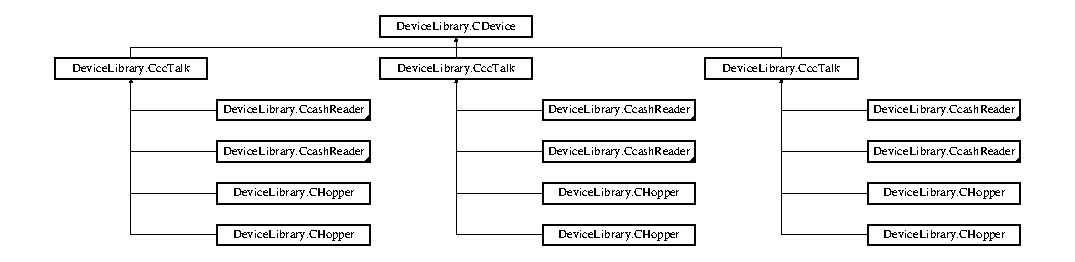
\includegraphics[height=3.076923cm]{class_device_library_1_1_c_device}
\end{center}
\end{figure}
\subsection*{Classes}
\begin{DoxyCompactItemize}
\item 
class \mbox{\hyperlink{class_device_library_1_1_c_device_1_1_c_inserted}{C\+Inserted}}
\begin{DoxyCompactList}\small\item\em Classe des pièces insérées \end{DoxyCompactList}\item 
class \mbox{\hyperlink{class_device_library_1_1_c_device_1_1_c_level}{C\+Level}}
\end{DoxyCompactItemize}
\subsection*{Public Member Functions}
\begin{DoxyCompactItemize}
\item 
\mbox{\hyperlink{class_device_library_1_1_c_device_a1ea11e47275e8d7baaa1f60a64c41d83}{C\+Device}} ()
\end{DoxyCompactItemize}
\subsection*{Public Attributes}
\begin{DoxyCompactItemize}
\item 
\mbox{\hyperlink{class_device_library_1_1_c_device_1_1_c_level}{C\+Level}} \mbox{\hyperlink{class_device_library_1_1_c_device_ae70218e48d761e45c66226ab7ea40e48}{device\+Level}}
\end{DoxyCompactItemize}
\subsection*{Static Public Attributes}
\begin{DoxyCompactItemize}
\item 
static \mbox{\hyperlink{class_device_library_1_1_c_device_1_1_c_inserted}{C\+Inserted}} \mbox{\hyperlink{class_device_library_1_1_c_device_aa37ddd8fa2c4edfc974ce0865e20d37a}{denomination\+Inserted}}
\end{DoxyCompactItemize}
\subsection*{Properties}
\begin{DoxyCompactItemize}
\item 
virtual int \mbox{\hyperlink{class_device_library_1_1_c_device_a5d542b0634e0024751d1e6df6975e0b8}{Serial\+Number}}\hspace{0.3cm}{\ttfamily  \mbox{[}get\mbox{]}}
\begin{DoxyCompactList}\small\item\em Numéro de série du périphérique \end{DoxyCompactList}\item 
abstract string \mbox{\hyperlink{class_device_library_1_1_c_device_a15613af54894a9dd673f76ac539741b1}{Manufacturer}}\hspace{0.3cm}{\ttfamily  \mbox{[}get\mbox{]}}
\begin{DoxyCompactList}\small\item\em Identifiant du fabricant \end{DoxyCompactList}\item 
abstract string \mbox{\hyperlink{class_device_library_1_1_c_device_adb37480555a37555da8fc17c73196fda}{Product\+Code}}\hspace{0.3cm}{\ttfamily  \mbox{[}get\mbox{]}}
\begin{DoxyCompactList}\small\item\em Fonction demandant le code produit \end{DoxyCompactList}\item 
bool \mbox{\hyperlink{class_device_library_1_1_c_device_a72aa72778cf6f58e44f7048f8f86fe2f}{Is\+Present}}\hspace{0.3cm}{\ttfamily  \mbox{[}get, set\mbox{]}}
\begin{DoxyCompactList}\small\item\em Flag indiquant si le hopper est detecté. \end{DoxyCompactList}\end{DoxyCompactItemize}


\subsection{Detailed Description}
Classe abstraite parent de tous les périphériques 



\subsection{Constructor \& Destructor Documentation}
\mbox{\Hypertarget{class_device_library_1_1_c_device_a1ea11e47275e8d7baaa1f60a64c41d83}\label{class_device_library_1_1_c_device_a1ea11e47275e8d7baaa1f60a64c41d83}} 
\index{Device\+Library\+::\+C\+Device@{Device\+Library\+::\+C\+Device}!C\+Device@{C\+Device}}
\index{C\+Device@{C\+Device}!Device\+Library\+::\+C\+Device@{Device\+Library\+::\+C\+Device}}
\subsubsection{\texorpdfstring{C\+Device()}{CDevice()}}
{\footnotesize\ttfamily Device\+Library.\+C\+Device.\+C\+Device (\begin{DoxyParamCaption}{ }\end{DoxyParamCaption})\hspace{0.3cm}{\ttfamily [inline]}}







\subsection{Member Data Documentation}
\mbox{\Hypertarget{class_device_library_1_1_c_device_aa37ddd8fa2c4edfc974ce0865e20d37a}\label{class_device_library_1_1_c_device_aa37ddd8fa2c4edfc974ce0865e20d37a}} 
\index{Device\+Library\+::\+C\+Device@{Device\+Library\+::\+C\+Device}!denomination\+Inserted@{denomination\+Inserted}}
\index{denomination\+Inserted@{denomination\+Inserted}!Device\+Library\+::\+C\+Device@{Device\+Library\+::\+C\+Device}}
\subsubsection{\texorpdfstring{denomination\+Inserted}{denominationInserted}}
{\footnotesize\ttfamily \mbox{\hyperlink{class_device_library_1_1_c_device_1_1_c_inserted}{C\+Inserted}} Device\+Library.\+C\+Device.\+denomination\+Inserted\hspace{0.3cm}{\ttfamily [static]}}





\mbox{\Hypertarget{class_device_library_1_1_c_device_ae70218e48d761e45c66226ab7ea40e48}\label{class_device_library_1_1_c_device_ae70218e48d761e45c66226ab7ea40e48}} 
\index{Device\+Library\+::\+C\+Device@{Device\+Library\+::\+C\+Device}!device\+Level@{device\+Level}}
\index{device\+Level@{device\+Level}!Device\+Library\+::\+C\+Device@{Device\+Library\+::\+C\+Device}}
\subsubsection{\texorpdfstring{device\+Level}{deviceLevel}}
{\footnotesize\ttfamily \mbox{\hyperlink{class_device_library_1_1_c_device_1_1_c_level}{C\+Level}} Device\+Library.\+C\+Device.\+device\+Level}







\subsection{Property Documentation}
\mbox{\Hypertarget{class_device_library_1_1_c_device_a72aa72778cf6f58e44f7048f8f86fe2f}\label{class_device_library_1_1_c_device_a72aa72778cf6f58e44f7048f8f86fe2f}} 
\index{Device\+Library\+::\+C\+Device@{Device\+Library\+::\+C\+Device}!Is\+Present@{Is\+Present}}
\index{Is\+Present@{Is\+Present}!Device\+Library\+::\+C\+Device@{Device\+Library\+::\+C\+Device}}
\subsubsection{\texorpdfstring{Is\+Present}{IsPresent}}
{\footnotesize\ttfamily bool Device\+Library.\+C\+Device.\+Is\+Present\hspace{0.3cm}{\ttfamily [get]}, {\ttfamily [set]}}



Flag indiquant si le hopper est detecté. 

\mbox{\Hypertarget{class_device_library_1_1_c_device_a15613af54894a9dd673f76ac539741b1}\label{class_device_library_1_1_c_device_a15613af54894a9dd673f76ac539741b1}} 
\index{Device\+Library\+::\+C\+Device@{Device\+Library\+::\+C\+Device}!Manufacturer@{Manufacturer}}
\index{Manufacturer@{Manufacturer}!Device\+Library\+::\+C\+Device@{Device\+Library\+::\+C\+Device}}
\subsubsection{\texorpdfstring{Manufacturer}{Manufacturer}}
{\footnotesize\ttfamily abstract string Device\+Library.\+C\+Device.\+Manufacturer\hspace{0.3cm}{\ttfamily [get]}}



Identifiant du fabricant 

\mbox{\Hypertarget{class_device_library_1_1_c_device_adb37480555a37555da8fc17c73196fda}\label{class_device_library_1_1_c_device_adb37480555a37555da8fc17c73196fda}} 
\index{Device\+Library\+::\+C\+Device@{Device\+Library\+::\+C\+Device}!Product\+Code@{Product\+Code}}
\index{Product\+Code@{Product\+Code}!Device\+Library\+::\+C\+Device@{Device\+Library\+::\+C\+Device}}
\subsubsection{\texorpdfstring{Product\+Code}{ProductCode}}
{\footnotesize\ttfamily abstract string Device\+Library.\+C\+Device.\+Product\+Code\hspace{0.3cm}{\ttfamily [get]}}



Fonction demandant le code produit 

\begin{DoxyReturn}{Returns}
Une chaîne de caractères contenant le code produit
\end{DoxyReturn}
\mbox{\Hypertarget{class_device_library_1_1_c_device_a5d542b0634e0024751d1e6df6975e0b8}\label{class_device_library_1_1_c_device_a5d542b0634e0024751d1e6df6975e0b8}} 
\index{Device\+Library\+::\+C\+Device@{Device\+Library\+::\+C\+Device}!Serial\+Number@{Serial\+Number}}
\index{Serial\+Number@{Serial\+Number}!Device\+Library\+::\+C\+Device@{Device\+Library\+::\+C\+Device}}
\subsubsection{\texorpdfstring{Serial\+Number}{SerialNumber}}
{\footnotesize\ttfamily virtual int Device\+Library.\+C\+Device.\+Serial\+Number\hspace{0.3cm}{\ttfamily [get]}}



Numéro de série du périphérique 



The documentation for this class was generated from the following file\+:\begin{DoxyCompactItemize}
\item 
D\+:/\+Projets/\+A\+T\+M\+B/\+S\+O\+F\+T/\+Atmb\+Devices/\+Device\+Library/C\+Device.\+cs\end{DoxyCompactItemize}

\hypertarget{class_device_library_1_1_c_devices_manage}{}\section{Device\+Library.\+C\+Devices\+Manage Class Reference}
\label{class_device_library_1_1_c_devices_manage}\index{Device\+Library.\+C\+Devices\+Manage@{Device\+Library.\+C\+Devices\+Manage}}


Class principale  


\subsection*{Public Member Functions}
\begin{DoxyCompactItemize}
\item 
delegate void \mbox{\hyperlink{class_device_library_1_1_c_devices_manage_a76f84b8a18500338f67d33123aa3332a}{Alert\+Event\+Handler}} (object sender, \mbox{\hyperlink{class_device_library_1_1_calert_event_args}{Calert\+Event\+Args}} e)
\item 
void \mbox{\hyperlink{class_device_library_1_1_c_devices_manage_a207100abcf87d3e21768d5284d84a100}{Open\+Transaction}} (int value)
\begin{DoxyCompactList}\small\item\em Ouvre une transaction le montant à payer. \end{DoxyCompactList}\item 
void \mbox{\hyperlink{class_device_library_1_1_c_devices_manage_a4bf7edbc6a2147169527ffa5b8233fc3}{Close\+Transaction}} ()
\begin{DoxyCompactList}\small\item\em Cloture la transaction en cours \end{DoxyCompactList}\item 
string \mbox{\hyperlink{class_device_library_1_1_c_devices_manage_a6b10aa601256c13d54c8c4642b029e10}{Get\+Serial\+Port}} ()
\begin{DoxyCompactList}\small\item\em Renvoi le nom du port série utilisé par le bus cc\+Talk \end{DoxyCompactList}\item 
\mbox{\hyperlink{class_device_library_1_1_c_devices_manage_a56177d99576c5d63e3233458a2a70ae1}{C\+Devices\+Manage}} ()
\begin{DoxyCompactList}\small\item\em Constructeur de la classe principale \end{DoxyCompactList}\item 
void \mbox{\hyperlink{class_device_library_1_1_c_devices_manage_a369960a1c585a85b637c7c217f927e1f}{Dispose}} ()
\begin{DoxyCompactList}\small\item\em Fonction libérant les ressources \end{DoxyCompactList}\end{DoxyCompactItemize}
\subsection*{Public Attributes}
\begin{DoxyCompactItemize}
\item 
\mbox{\hyperlink{class_device_library_1_1_c_coin_validator}{C\+Coin\+Validator}} \mbox{\hyperlink{class_device_library_1_1_c_devices_manage_a0a0fd3a37a1a8c01b2227b3cd0029b11}{monnayeur}}
\begin{DoxyCompactList}\small\item\em Instance du monnayeur \end{DoxyCompactList}\item 
List$<$ \mbox{\hyperlink{class_device_library_1_1_c_hopper}{C\+Hopper}} $>$ \mbox{\hyperlink{class_device_library_1_1_c_devices_manage_ae9d4323b152f0a1767c004668d2ab3ea}{Hoppers}}
\begin{DoxyCompactList}\small\item\em Liste des hoppers \end{DoxyCompactList}\end{DoxyCompactItemize}
\subsection*{Properties}
\begin{DoxyCompactItemize}
\item 
static byte \mbox{[}$\,$\mbox{]} \mbox{\hyperlink{class_device_library_1_1_c_devices_manage_a881da4fa7a164664f6342669ca532b7b}{Enable\+Channels}}\hspace{0.3cm}{\ttfamily  \mbox{[}get\mbox{]}}
\begin{DoxyCompactList}\small\item\em Masque des canaux activés. \end{DoxyCompactList}\end{DoxyCompactItemize}
\subsection*{Events}
\begin{DoxyCompactItemize}
\item 
\mbox{\hyperlink{class_device_library_1_1_c_devices_manage_a76f84b8a18500338f67d33123aa3332a}{Alert\+Event\+Handler}} \mbox{\hyperlink{class_device_library_1_1_c_devices_manage_a6813f81d6f606f0aa66fb6613af6bbe8}{Call\+Alert}}
\begin{DoxyCompactList}\small\item\em Evenement levant un appel à la fonction déléguée. \end{DoxyCompactList}\end{DoxyCompactItemize}


\subsection{Detailed Description}
Class principale 



\subsection{Constructor \& Destructor Documentation}
\mbox{\Hypertarget{class_device_library_1_1_c_devices_manage_a56177d99576c5d63e3233458a2a70ae1}\label{class_device_library_1_1_c_devices_manage_a56177d99576c5d63e3233458a2a70ae1}} 
\index{Device\+Library\+::\+C\+Devices\+Manage@{Device\+Library\+::\+C\+Devices\+Manage}!C\+Devices\+Manage@{C\+Devices\+Manage}}
\index{C\+Devices\+Manage@{C\+Devices\+Manage}!Device\+Library\+::\+C\+Devices\+Manage@{Device\+Library\+::\+C\+Devices\+Manage}}
\subsubsection{\texorpdfstring{C\+Devices\+Manage()}{CDevicesManage()}}
{\footnotesize\ttfamily Device\+Library.\+C\+Devices\+Manage.\+C\+Devices\+Manage (\begin{DoxyParamCaption}{ }\end{DoxyParamCaption})\hspace{0.3cm}{\ttfamily [inline]}}



Constructeur de la classe principale 



\subsection{Member Function Documentation}
\mbox{\Hypertarget{class_device_library_1_1_c_devices_manage_a76f84b8a18500338f67d33123aa3332a}\label{class_device_library_1_1_c_devices_manage_a76f84b8a18500338f67d33123aa3332a}} 
\index{Device\+Library\+::\+C\+Devices\+Manage@{Device\+Library\+::\+C\+Devices\+Manage}!Alert\+Event\+Handler@{Alert\+Event\+Handler}}
\index{Alert\+Event\+Handler@{Alert\+Event\+Handler}!Device\+Library\+::\+C\+Devices\+Manage@{Device\+Library\+::\+C\+Devices\+Manage}}
\subsubsection{\texorpdfstring{Alert\+Event\+Handler()}{AlertEventHandler()}}
{\footnotesize\ttfamily delegate void Device\+Library.\+C\+Devices\+Manage.\+Alert\+Event\+Handler (\begin{DoxyParamCaption}\item[{object}]{sender,  }\item[{\mbox{\hyperlink{class_device_library_1_1_calert_event_args}{Calert\+Event\+Args}}}]{e }\end{DoxyParamCaption})}






\begin{DoxyParams}{Parameters}
{\em sender} & \\
\hline
{\em e} & \\
\hline
\end{DoxyParams}
\mbox{\Hypertarget{class_device_library_1_1_c_devices_manage_a4bf7edbc6a2147169527ffa5b8233fc3}\label{class_device_library_1_1_c_devices_manage_a4bf7edbc6a2147169527ffa5b8233fc3}} 
\index{Device\+Library\+::\+C\+Devices\+Manage@{Device\+Library\+::\+C\+Devices\+Manage}!Close\+Transaction@{Close\+Transaction}}
\index{Close\+Transaction@{Close\+Transaction}!Device\+Library\+::\+C\+Devices\+Manage@{Device\+Library\+::\+C\+Devices\+Manage}}
\subsubsection{\texorpdfstring{Close\+Transaction()}{CloseTransaction()}}
{\footnotesize\ttfamily void Device\+Library.\+C\+Devices\+Manage.\+Close\+Transaction (\begin{DoxyParamCaption}{ }\end{DoxyParamCaption})\hspace{0.3cm}{\ttfamily [inline]}}



Cloture la transaction en cours 

\mbox{\Hypertarget{class_device_library_1_1_c_devices_manage_a369960a1c585a85b637c7c217f927e1f}\label{class_device_library_1_1_c_devices_manage_a369960a1c585a85b637c7c217f927e1f}} 
\index{Device\+Library\+::\+C\+Devices\+Manage@{Device\+Library\+::\+C\+Devices\+Manage}!Dispose@{Dispose}}
\index{Dispose@{Dispose}!Device\+Library\+::\+C\+Devices\+Manage@{Device\+Library\+::\+C\+Devices\+Manage}}
\subsubsection{\texorpdfstring{Dispose()}{Dispose()}}
{\footnotesize\ttfamily void Device\+Library.\+C\+Devices\+Manage.\+Dispose (\begin{DoxyParamCaption}{ }\end{DoxyParamCaption})\hspace{0.3cm}{\ttfamily [inline]}}



Fonction libérant les ressources 

\mbox{\Hypertarget{class_device_library_1_1_c_devices_manage_a6b10aa601256c13d54c8c4642b029e10}\label{class_device_library_1_1_c_devices_manage_a6b10aa601256c13d54c8c4642b029e10}} 
\index{Device\+Library\+::\+C\+Devices\+Manage@{Device\+Library\+::\+C\+Devices\+Manage}!Get\+Serial\+Port@{Get\+Serial\+Port}}
\index{Get\+Serial\+Port@{Get\+Serial\+Port}!Device\+Library\+::\+C\+Devices\+Manage@{Device\+Library\+::\+C\+Devices\+Manage}}
\subsubsection{\texorpdfstring{Get\+Serial\+Port()}{GetSerialPort()}}
{\footnotesize\ttfamily string Device\+Library.\+C\+Devices\+Manage.\+Get\+Serial\+Port (\begin{DoxyParamCaption}{ }\end{DoxyParamCaption})\hspace{0.3cm}{\ttfamily [inline]}}



Renvoi le nom du port série utilisé par le bus cc\+Talk 

\mbox{\Hypertarget{class_device_library_1_1_c_devices_manage_a207100abcf87d3e21768d5284d84a100}\label{class_device_library_1_1_c_devices_manage_a207100abcf87d3e21768d5284d84a100}} 
\index{Device\+Library\+::\+C\+Devices\+Manage@{Device\+Library\+::\+C\+Devices\+Manage}!Open\+Transaction@{Open\+Transaction}}
\index{Open\+Transaction@{Open\+Transaction}!Device\+Library\+::\+C\+Devices\+Manage@{Device\+Library\+::\+C\+Devices\+Manage}}
\subsubsection{\texorpdfstring{Open\+Transaction()}{OpenTransaction()}}
{\footnotesize\ttfamily void Device\+Library.\+C\+Devices\+Manage.\+Open\+Transaction (\begin{DoxyParamCaption}\item[{int}]{value }\end{DoxyParamCaption})\hspace{0.3cm}{\ttfamily [inline]}}



Ouvre une transaction le montant à payer. 


\begin{DoxyParams}{Parameters}
{\em value} & montant en centimes à payer\\
\hline
\end{DoxyParams}


Provoque l\textquotesingle{}ouverture des moyens de paiement.

\subsection{Member Data Documentation}
\mbox{\Hypertarget{class_device_library_1_1_c_devices_manage_ae9d4323b152f0a1767c004668d2ab3ea}\label{class_device_library_1_1_c_devices_manage_ae9d4323b152f0a1767c004668d2ab3ea}} 
\index{Device\+Library\+::\+C\+Devices\+Manage@{Device\+Library\+::\+C\+Devices\+Manage}!Hoppers@{Hoppers}}
\index{Hoppers@{Hoppers}!Device\+Library\+::\+C\+Devices\+Manage@{Device\+Library\+::\+C\+Devices\+Manage}}
\subsubsection{\texorpdfstring{Hoppers}{Hoppers}}
{\footnotesize\ttfamily List$<$\mbox{\hyperlink{class_device_library_1_1_c_hopper}{C\+Hopper}}$>$ Device\+Library.\+C\+Devices\+Manage.\+Hoppers}



Liste des hoppers 

\mbox{\Hypertarget{class_device_library_1_1_c_devices_manage_a0a0fd3a37a1a8c01b2227b3cd0029b11}\label{class_device_library_1_1_c_devices_manage_a0a0fd3a37a1a8c01b2227b3cd0029b11}} 
\index{Device\+Library\+::\+C\+Devices\+Manage@{Device\+Library\+::\+C\+Devices\+Manage}!monnayeur@{monnayeur}}
\index{monnayeur@{monnayeur}!Device\+Library\+::\+C\+Devices\+Manage@{Device\+Library\+::\+C\+Devices\+Manage}}
\subsubsection{\texorpdfstring{monnayeur}{monnayeur}}
{\footnotesize\ttfamily \mbox{\hyperlink{class_device_library_1_1_c_coin_validator}{C\+Coin\+Validator}} Device\+Library.\+C\+Devices\+Manage.\+monnayeur}



Instance du monnayeur 



\subsection{Property Documentation}
\mbox{\Hypertarget{class_device_library_1_1_c_devices_manage_a881da4fa7a164664f6342669ca532b7b}\label{class_device_library_1_1_c_devices_manage_a881da4fa7a164664f6342669ca532b7b}} 
\index{Device\+Library\+::\+C\+Devices\+Manage@{Device\+Library\+::\+C\+Devices\+Manage}!Enable\+Channels@{Enable\+Channels}}
\index{Enable\+Channels@{Enable\+Channels}!Device\+Library\+::\+C\+Devices\+Manage@{Device\+Library\+::\+C\+Devices\+Manage}}
\subsubsection{\texorpdfstring{Enable\+Channels}{EnableChannels}}
{\footnotesize\ttfamily byte \mbox{[}$\,$\mbox{]} Device\+Library.\+C\+Devices\+Manage.\+Enable\+Channels\hspace{0.3cm}{\ttfamily [static]}, {\ttfamily [get]}}



Masque des canaux activés. 



\subsection{Event Documentation}
\mbox{\Hypertarget{class_device_library_1_1_c_devices_manage_a6813f81d6f606f0aa66fb6613af6bbe8}\label{class_device_library_1_1_c_devices_manage_a6813f81d6f606f0aa66fb6613af6bbe8}} 
\index{Device\+Library\+::\+C\+Devices\+Manage@{Device\+Library\+::\+C\+Devices\+Manage}!Call\+Alert@{Call\+Alert}}
\index{Call\+Alert@{Call\+Alert}!Device\+Library\+::\+C\+Devices\+Manage@{Device\+Library\+::\+C\+Devices\+Manage}}
\subsubsection{\texorpdfstring{Call\+Alert}{CallAlert}}
{\footnotesize\ttfamily \mbox{\hyperlink{class_device_library_1_1_c_devices_manage_a76f84b8a18500338f67d33123aa3332a}{Alert\+Event\+Handler}} Device\+Library.\+C\+Devices\+Manage.\+Call\+Alert}



Evenement levant un appel à la fonction déléguée. 



The documentation for this class was generated from the following file\+:\begin{DoxyCompactItemize}
\item 
D\+:/\+Projets/\+A\+T\+M\+B/\+S\+O\+F\+T/\+Atmb\+Devices/\+Device\+Library/C\+Devices\+Manage.\+cs\end{DoxyCompactItemize}

\hypertarget{class_device_library_1_1_c_hopper_1_1_c_hopper_status_1_1_c_dispensed_result}{}\section{Device\+Library.\+C\+Hopper.\+C\+Hopper\+Status.\+C\+Dispensed\+Result Class Reference}
\label{class_device_library_1_1_c_hopper_1_1_c_hopper_status_1_1_c_dispensed_result}\index{Device\+Library.\+C\+Hopper.\+C\+Hopper\+Status.\+C\+Dispensed\+Result@{Device\+Library.\+C\+Hopper.\+C\+Hopper\+Status.\+C\+Dispensed\+Result}}


Classe des resultats d\textquotesingle{}une distribution.  


\subsection*{Public Member Functions}
\begin{DoxyCompactItemize}
\item 
\mbox{\hyperlink{class_device_library_1_1_c_hopper_1_1_c_hopper_status_1_1_c_dispensed_result_afe0fb651efeaf2009052a6f45f64dbbe}{C\+Dispensed\+Result}} (byte hopper\+Number)
\begin{DoxyCompactList}\small\item\em Constructeur \end{DoxyCompactList}\end{DoxyCompactItemize}
\subsection*{Public Attributes}
\begin{DoxyCompactItemize}
\item 
byte \mbox{\hyperlink{class_device_library_1_1_c_hopper_1_1_c_hopper_status_1_1_c_dispensed_result_aea7d1e629abb83dbd02478d04547278d}{Hopper\+Number}}
\begin{DoxyCompactList}\small\item\em Numéro du hopper. \end{DoxyCompactList}\item 
byte \mbox{\hyperlink{class_device_library_1_1_c_hopper_1_1_c_hopper_status_1_1_c_dispensed_result_a2eac4efe6ef793ea361f0f2c5baf5326}{Coins\+Remaining}}
\begin{DoxyCompactList}\small\item\em Nombre de pièce restant à payer. \end{DoxyCompactList}\item 
byte \mbox{\hyperlink{class_device_library_1_1_c_hopper_1_1_c_hopper_status_1_1_c_dispensed_result_a8266bc3a0c5a4c268d57f5ed83d0882f}{Coins\+Paid}}
\begin{DoxyCompactList}\small\item\em Nombre de pièces distribuées. \end{DoxyCompactList}\item 
byte \mbox{\hyperlink{class_device_library_1_1_c_hopper_1_1_c_hopper_status_1_1_c_dispensed_result_a2a472fae256a38b6fa595a8a2047a4c6}{Coins\+Unpaid}}
\begin{DoxyCompactList}\small\item\em Nombre de pièces non distribuées \end{DoxyCompactList}\item 
int \mbox{\hyperlink{class_device_library_1_1_c_hopper_1_1_c_hopper_status_1_1_c_dispensed_result_a575da9fcadfa091789d482ce63a10d6f}{Montant\+Paid}}
\begin{DoxyCompactList}\small\item\em Montant distribué \end{DoxyCompactList}\item 
int \mbox{\hyperlink{class_device_library_1_1_c_hopper_1_1_c_hopper_status_1_1_c_dispensed_result_a0c4e306c0e2bfd89d578c4de56978f70}{Montant\+Unpaid}}
\begin{DoxyCompactList}\small\item\em Montant non distribué \end{DoxyCompactList}\item 
byte \mbox{\hyperlink{class_device_library_1_1_c_hopper_1_1_c_hopper_status_1_1_c_dispensed_result_a6aae05e36efc56b7879b36cae19836fd}{Coin\+To\+Dispense}}
\begin{DoxyCompactList}\small\item\em Nombre de pièces devant être distribuées \end{DoxyCompactList}\item 
int \mbox{\hyperlink{class_device_library_1_1_c_hopper_1_1_c_hopper_status_1_1_c_dispensed_result_a50cf9d9c803868a3d5df1a5359c4efd4}{Amount\+To\+Dispense}}
\begin{DoxyCompactList}\small\item\em Montant \end{DoxyCompactList}\end{DoxyCompactItemize}


\subsection{Detailed Description}
Classe des resultats d\textquotesingle{}une distribution. 



\subsection{Constructor \& Destructor Documentation}
\mbox{\Hypertarget{class_device_library_1_1_c_hopper_1_1_c_hopper_status_1_1_c_dispensed_result_afe0fb651efeaf2009052a6f45f64dbbe}\label{class_device_library_1_1_c_hopper_1_1_c_hopper_status_1_1_c_dispensed_result_afe0fb651efeaf2009052a6f45f64dbbe}} 
\index{Device\+Library\+::\+C\+Hopper\+::\+C\+Hopper\+Status\+::\+C\+Dispensed\+Result@{Device\+Library\+::\+C\+Hopper\+::\+C\+Hopper\+Status\+::\+C\+Dispensed\+Result}!C\+Dispensed\+Result@{C\+Dispensed\+Result}}
\index{C\+Dispensed\+Result@{C\+Dispensed\+Result}!Device\+Library\+::\+C\+Hopper\+::\+C\+Hopper\+Status\+::\+C\+Dispensed\+Result@{Device\+Library\+::\+C\+Hopper\+::\+C\+Hopper\+Status\+::\+C\+Dispensed\+Result}}
\subsubsection{\texorpdfstring{C\+Dispensed\+Result()}{CDispensedResult()}}
{\footnotesize\ttfamily Device\+Library.\+C\+Hopper.\+C\+Hopper\+Status.\+C\+Dispensed\+Result.\+C\+Dispensed\+Result (\begin{DoxyParamCaption}\item[{byte}]{hopper\+Number }\end{DoxyParamCaption})\hspace{0.3cm}{\ttfamily [inline]}}



Constructeur 


\begin{DoxyParams}{Parameters}
{\em hopper\+Number} & \\
\hline
\end{DoxyParams}


\subsection{Member Data Documentation}
\mbox{\Hypertarget{class_device_library_1_1_c_hopper_1_1_c_hopper_status_1_1_c_dispensed_result_a50cf9d9c803868a3d5df1a5359c4efd4}\label{class_device_library_1_1_c_hopper_1_1_c_hopper_status_1_1_c_dispensed_result_a50cf9d9c803868a3d5df1a5359c4efd4}} 
\index{Device\+Library\+::\+C\+Hopper\+::\+C\+Hopper\+Status\+::\+C\+Dispensed\+Result@{Device\+Library\+::\+C\+Hopper\+::\+C\+Hopper\+Status\+::\+C\+Dispensed\+Result}!Amount\+To\+Dispense@{Amount\+To\+Dispense}}
\index{Amount\+To\+Dispense@{Amount\+To\+Dispense}!Device\+Library\+::\+C\+Hopper\+::\+C\+Hopper\+Status\+::\+C\+Dispensed\+Result@{Device\+Library\+::\+C\+Hopper\+::\+C\+Hopper\+Status\+::\+C\+Dispensed\+Result}}
\subsubsection{\texorpdfstring{Amount\+To\+Dispense}{AmountToDispense}}
{\footnotesize\ttfamily int Device\+Library.\+C\+Hopper.\+C\+Hopper\+Status.\+C\+Dispensed\+Result.\+Amount\+To\+Dispense}



Montant 

\mbox{\Hypertarget{class_device_library_1_1_c_hopper_1_1_c_hopper_status_1_1_c_dispensed_result_a8266bc3a0c5a4c268d57f5ed83d0882f}\label{class_device_library_1_1_c_hopper_1_1_c_hopper_status_1_1_c_dispensed_result_a8266bc3a0c5a4c268d57f5ed83d0882f}} 
\index{Device\+Library\+::\+C\+Hopper\+::\+C\+Hopper\+Status\+::\+C\+Dispensed\+Result@{Device\+Library\+::\+C\+Hopper\+::\+C\+Hopper\+Status\+::\+C\+Dispensed\+Result}!Coins\+Paid@{Coins\+Paid}}
\index{Coins\+Paid@{Coins\+Paid}!Device\+Library\+::\+C\+Hopper\+::\+C\+Hopper\+Status\+::\+C\+Dispensed\+Result@{Device\+Library\+::\+C\+Hopper\+::\+C\+Hopper\+Status\+::\+C\+Dispensed\+Result}}
\subsubsection{\texorpdfstring{Coins\+Paid}{CoinsPaid}}
{\footnotesize\ttfamily byte Device\+Library.\+C\+Hopper.\+C\+Hopper\+Status.\+C\+Dispensed\+Result.\+Coins\+Paid}



Nombre de pièces distribuées. 

\mbox{\Hypertarget{class_device_library_1_1_c_hopper_1_1_c_hopper_status_1_1_c_dispensed_result_a2eac4efe6ef793ea361f0f2c5baf5326}\label{class_device_library_1_1_c_hopper_1_1_c_hopper_status_1_1_c_dispensed_result_a2eac4efe6ef793ea361f0f2c5baf5326}} 
\index{Device\+Library\+::\+C\+Hopper\+::\+C\+Hopper\+Status\+::\+C\+Dispensed\+Result@{Device\+Library\+::\+C\+Hopper\+::\+C\+Hopper\+Status\+::\+C\+Dispensed\+Result}!Coins\+Remaining@{Coins\+Remaining}}
\index{Coins\+Remaining@{Coins\+Remaining}!Device\+Library\+::\+C\+Hopper\+::\+C\+Hopper\+Status\+::\+C\+Dispensed\+Result@{Device\+Library\+::\+C\+Hopper\+::\+C\+Hopper\+Status\+::\+C\+Dispensed\+Result}}
\subsubsection{\texorpdfstring{Coins\+Remaining}{CoinsRemaining}}
{\footnotesize\ttfamily byte Device\+Library.\+C\+Hopper.\+C\+Hopper\+Status.\+C\+Dispensed\+Result.\+Coins\+Remaining}



Nombre de pièce restant à payer. 

remarks$>$Passe à zéro à la fin de la distribtion quelque soit la raison.\mbox{\Hypertarget{class_device_library_1_1_c_hopper_1_1_c_hopper_status_1_1_c_dispensed_result_a2a472fae256a38b6fa595a8a2047a4c6}\label{class_device_library_1_1_c_hopper_1_1_c_hopper_status_1_1_c_dispensed_result_a2a472fae256a38b6fa595a8a2047a4c6}} 
\index{Device\+Library\+::\+C\+Hopper\+::\+C\+Hopper\+Status\+::\+C\+Dispensed\+Result@{Device\+Library\+::\+C\+Hopper\+::\+C\+Hopper\+Status\+::\+C\+Dispensed\+Result}!Coins\+Unpaid@{Coins\+Unpaid}}
\index{Coins\+Unpaid@{Coins\+Unpaid}!Device\+Library\+::\+C\+Hopper\+::\+C\+Hopper\+Status\+::\+C\+Dispensed\+Result@{Device\+Library\+::\+C\+Hopper\+::\+C\+Hopper\+Status\+::\+C\+Dispensed\+Result}}
\subsubsection{\texorpdfstring{Coins\+Unpaid}{CoinsUnpaid}}
{\footnotesize\ttfamily byte Device\+Library.\+C\+Hopper.\+C\+Hopper\+Status.\+C\+Dispensed\+Result.\+Coins\+Unpaid}



Nombre de pièces non distribuées 

\mbox{\Hypertarget{class_device_library_1_1_c_hopper_1_1_c_hopper_status_1_1_c_dispensed_result_a6aae05e36efc56b7879b36cae19836fd}\label{class_device_library_1_1_c_hopper_1_1_c_hopper_status_1_1_c_dispensed_result_a6aae05e36efc56b7879b36cae19836fd}} 
\index{Device\+Library\+::\+C\+Hopper\+::\+C\+Hopper\+Status\+::\+C\+Dispensed\+Result@{Device\+Library\+::\+C\+Hopper\+::\+C\+Hopper\+Status\+::\+C\+Dispensed\+Result}!Coin\+To\+Dispense@{Coin\+To\+Dispense}}
\index{Coin\+To\+Dispense@{Coin\+To\+Dispense}!Device\+Library\+::\+C\+Hopper\+::\+C\+Hopper\+Status\+::\+C\+Dispensed\+Result@{Device\+Library\+::\+C\+Hopper\+::\+C\+Hopper\+Status\+::\+C\+Dispensed\+Result}}
\subsubsection{\texorpdfstring{Coin\+To\+Dispense}{CoinToDispense}}
{\footnotesize\ttfamily byte Device\+Library.\+C\+Hopper.\+C\+Hopper\+Status.\+C\+Dispensed\+Result.\+Coin\+To\+Dispense}



Nombre de pièces devant être distribuées 

\mbox{\Hypertarget{class_device_library_1_1_c_hopper_1_1_c_hopper_status_1_1_c_dispensed_result_aea7d1e629abb83dbd02478d04547278d}\label{class_device_library_1_1_c_hopper_1_1_c_hopper_status_1_1_c_dispensed_result_aea7d1e629abb83dbd02478d04547278d}} 
\index{Device\+Library\+::\+C\+Hopper\+::\+C\+Hopper\+Status\+::\+C\+Dispensed\+Result@{Device\+Library\+::\+C\+Hopper\+::\+C\+Hopper\+Status\+::\+C\+Dispensed\+Result}!Hopper\+Number@{Hopper\+Number}}
\index{Hopper\+Number@{Hopper\+Number}!Device\+Library\+::\+C\+Hopper\+::\+C\+Hopper\+Status\+::\+C\+Dispensed\+Result@{Device\+Library\+::\+C\+Hopper\+::\+C\+Hopper\+Status\+::\+C\+Dispensed\+Result}}
\subsubsection{\texorpdfstring{Hopper\+Number}{HopperNumber}}
{\footnotesize\ttfamily byte Device\+Library.\+C\+Hopper.\+C\+Hopper\+Status.\+C\+Dispensed\+Result.\+Hopper\+Number}



Numéro du hopper. 

\mbox{\Hypertarget{class_device_library_1_1_c_hopper_1_1_c_hopper_status_1_1_c_dispensed_result_a575da9fcadfa091789d482ce63a10d6f}\label{class_device_library_1_1_c_hopper_1_1_c_hopper_status_1_1_c_dispensed_result_a575da9fcadfa091789d482ce63a10d6f}} 
\index{Device\+Library\+::\+C\+Hopper\+::\+C\+Hopper\+Status\+::\+C\+Dispensed\+Result@{Device\+Library\+::\+C\+Hopper\+::\+C\+Hopper\+Status\+::\+C\+Dispensed\+Result}!Montant\+Paid@{Montant\+Paid}}
\index{Montant\+Paid@{Montant\+Paid}!Device\+Library\+::\+C\+Hopper\+::\+C\+Hopper\+Status\+::\+C\+Dispensed\+Result@{Device\+Library\+::\+C\+Hopper\+::\+C\+Hopper\+Status\+::\+C\+Dispensed\+Result}}
\subsubsection{\texorpdfstring{Montant\+Paid}{MontantPaid}}
{\footnotesize\ttfamily int Device\+Library.\+C\+Hopper.\+C\+Hopper\+Status.\+C\+Dispensed\+Result.\+Montant\+Paid}



Montant distribué 

\mbox{\Hypertarget{class_device_library_1_1_c_hopper_1_1_c_hopper_status_1_1_c_dispensed_result_a0c4e306c0e2bfd89d578c4de56978f70}\label{class_device_library_1_1_c_hopper_1_1_c_hopper_status_1_1_c_dispensed_result_a0c4e306c0e2bfd89d578c4de56978f70}} 
\index{Device\+Library\+::\+C\+Hopper\+::\+C\+Hopper\+Status\+::\+C\+Dispensed\+Result@{Device\+Library\+::\+C\+Hopper\+::\+C\+Hopper\+Status\+::\+C\+Dispensed\+Result}!Montant\+Unpaid@{Montant\+Unpaid}}
\index{Montant\+Unpaid@{Montant\+Unpaid}!Device\+Library\+::\+C\+Hopper\+::\+C\+Hopper\+Status\+::\+C\+Dispensed\+Result@{Device\+Library\+::\+C\+Hopper\+::\+C\+Hopper\+Status\+::\+C\+Dispensed\+Result}}
\subsubsection{\texorpdfstring{Montant\+Unpaid}{MontantUnpaid}}
{\footnotesize\ttfamily int Device\+Library.\+C\+Hopper.\+C\+Hopper\+Status.\+C\+Dispensed\+Result.\+Montant\+Unpaid}



Montant non distribué 



The documentation for this class was generated from the following file\+:\begin{DoxyCompactItemize}
\item 
D\+:/\+Projets/\+A\+T\+M\+B/\+S\+O\+F\+T/\+Atmb\+Devices/\+Device\+Library/C\+Hopper\+Status.\+cs\end{DoxyCompactItemize}

\hypertarget{class_device_library_1_1_c_hopper_1_1_c_empty_count}{}\section{Device\+Library.\+C\+Hopper.\+C\+Empty\+Count Class Reference}
\label{class_device_library_1_1_c_hopper_1_1_c_empty_count}\index{Device\+Library.\+C\+Hopper.\+C\+Empty\+Count@{Device\+Library.\+C\+Hopper.\+C\+Empty\+Count}}


Class contenant les résultats du vidage du hopper.  


\subsection*{Public Attributes}
\begin{DoxyCompactItemize}
\item 
long \mbox{\hyperlink{class_device_library_1_1_c_hopper_1_1_c_empty_count_a8ccb96ba708ceb8206e3ba99ebb201da}{counter}}
\begin{DoxyCompactList}\small\item\em Nombre de pièces comptées durant le vidage \end{DoxyCompactList}\item 
long \mbox{\hyperlink{class_device_library_1_1_c_hopper_1_1_c_empty_count_aa9438d053793ad17dfaaba410dff2af1}{amount\+Counter}}
\begin{DoxyCompactList}\small\item\em Montant distribué pendant le vidage. \end{DoxyCompactList}\item 
long \mbox{\hyperlink{class_device_library_1_1_c_hopper_1_1_c_empty_count_adf61aa1680a4934d9e2e6ebc47734e5a}{delta}}
\begin{DoxyCompactList}\small\item\em Différence entre le nombre de pièces dans les compteurs et le nombre de pièces distribuées pendant le vidage. \end{DoxyCompactList}\item 
long \mbox{\hyperlink{class_device_library_1_1_c_hopper_1_1_c_empty_count_a30e4ea7873f253cbaa362dac6985043b}{amount\+Delta}}
\begin{DoxyCompactList}\small\item\em Différence entre le montant distribué et le montant dans les compteurs. \end{DoxyCompactList}\end{DoxyCompactItemize}


\subsection{Detailed Description}
Class contenant les résultats du vidage du hopper. 



\subsection{Member Data Documentation}
\mbox{\Hypertarget{class_device_library_1_1_c_hopper_1_1_c_empty_count_aa9438d053793ad17dfaaba410dff2af1}\label{class_device_library_1_1_c_hopper_1_1_c_empty_count_aa9438d053793ad17dfaaba410dff2af1}} 
\index{Device\+Library\+::\+C\+Hopper\+::\+C\+Empty\+Count@{Device\+Library\+::\+C\+Hopper\+::\+C\+Empty\+Count}!amount\+Counter@{amount\+Counter}}
\index{amount\+Counter@{amount\+Counter}!Device\+Library\+::\+C\+Hopper\+::\+C\+Empty\+Count@{Device\+Library\+::\+C\+Hopper\+::\+C\+Empty\+Count}}
\subsubsection{\texorpdfstring{amount\+Counter}{amountCounter}}
{\footnotesize\ttfamily long Device\+Library.\+C\+Hopper.\+C\+Empty\+Count.\+amount\+Counter}



Montant distribué pendant le vidage. 

\mbox{\Hypertarget{class_device_library_1_1_c_hopper_1_1_c_empty_count_a30e4ea7873f253cbaa362dac6985043b}\label{class_device_library_1_1_c_hopper_1_1_c_empty_count_a30e4ea7873f253cbaa362dac6985043b}} 
\index{Device\+Library\+::\+C\+Hopper\+::\+C\+Empty\+Count@{Device\+Library\+::\+C\+Hopper\+::\+C\+Empty\+Count}!amount\+Delta@{amount\+Delta}}
\index{amount\+Delta@{amount\+Delta}!Device\+Library\+::\+C\+Hopper\+::\+C\+Empty\+Count@{Device\+Library\+::\+C\+Hopper\+::\+C\+Empty\+Count}}
\subsubsection{\texorpdfstring{amount\+Delta}{amountDelta}}
{\footnotesize\ttfamily long Device\+Library.\+C\+Hopper.\+C\+Empty\+Count.\+amount\+Delta}



Différence entre le montant distribué et le montant dans les compteurs. 

\mbox{\Hypertarget{class_device_library_1_1_c_hopper_1_1_c_empty_count_a8ccb96ba708ceb8206e3ba99ebb201da}\label{class_device_library_1_1_c_hopper_1_1_c_empty_count_a8ccb96ba708ceb8206e3ba99ebb201da}} 
\index{Device\+Library\+::\+C\+Hopper\+::\+C\+Empty\+Count@{Device\+Library\+::\+C\+Hopper\+::\+C\+Empty\+Count}!counter@{counter}}
\index{counter@{counter}!Device\+Library\+::\+C\+Hopper\+::\+C\+Empty\+Count@{Device\+Library\+::\+C\+Hopper\+::\+C\+Empty\+Count}}
\subsubsection{\texorpdfstring{counter}{counter}}
{\footnotesize\ttfamily long Device\+Library.\+C\+Hopper.\+C\+Empty\+Count.\+counter}



Nombre de pièces comptées durant le vidage 

\mbox{\Hypertarget{class_device_library_1_1_c_hopper_1_1_c_empty_count_adf61aa1680a4934d9e2e6ebc47734e5a}\label{class_device_library_1_1_c_hopper_1_1_c_empty_count_adf61aa1680a4934d9e2e6ebc47734e5a}} 
\index{Device\+Library\+::\+C\+Hopper\+::\+C\+Empty\+Count@{Device\+Library\+::\+C\+Hopper\+::\+C\+Empty\+Count}!delta@{delta}}
\index{delta@{delta}!Device\+Library\+::\+C\+Hopper\+::\+C\+Empty\+Count@{Device\+Library\+::\+C\+Hopper\+::\+C\+Empty\+Count}}
\subsubsection{\texorpdfstring{delta}{delta}}
{\footnotesize\ttfamily long Device\+Library.\+C\+Hopper.\+C\+Empty\+Count.\+delta}



Différence entre le nombre de pièces dans les compteurs et le nombre de pièces distribuées pendant le vidage. 



The documentation for this class was generated from the following file\+:\begin{DoxyCompactItemize}
\item 
D\+:/\+Projets/\+A\+T\+M\+B/\+S\+O\+F\+T/\+Atmb\+Devices/\+Device\+Library/C\+Hopper.\+cs\end{DoxyCompactItemize}

\hypertarget{class_device_library_1_1_c_coin_validator_1_1_c_erro_c_v}{}\section{Device\+Library.\+C\+Coin\+Validator.\+C\+Erro\+CV Class Reference}
\label{class_device_library_1_1_c_coin_validator_1_1_c_erro_c_v}\index{Device\+Library.\+C\+Coin\+Validator.\+C\+Erro\+CV@{Device\+Library.\+C\+Coin\+Validator.\+C\+Erro\+CV}}


 


\subsection*{Public Attributes}
\begin{DoxyCompactItemize}
\item 
byte \mbox{\hyperlink{class_device_library_1_1_c_coin_validator_1_1_c_erro_c_v_a645b37f5a1414ee05ef237a4afbd8e43}{code}}
\item 
\mbox{\hyperlink{group___erreur_ga68c5b73cc3b337502d9f92154d933591}{C\+V\+Error\+Codes}} \mbox{\hyperlink{class_device_library_1_1_c_coin_validator_1_1_c_erro_c_v_a0d512c6ac4b9a6e46c8161b4e9cf9828}{error\+Text}}
\end{DoxyCompactItemize}


\subsection{Detailed Description}




\subsection{Member Data Documentation}
\mbox{\Hypertarget{class_device_library_1_1_c_coin_validator_1_1_c_erro_c_v_a645b37f5a1414ee05ef237a4afbd8e43}\label{class_device_library_1_1_c_coin_validator_1_1_c_erro_c_v_a645b37f5a1414ee05ef237a4afbd8e43}} 
\index{Device\+Library\+::\+C\+Coin\+Validator\+::\+C\+Erro\+CV@{Device\+Library\+::\+C\+Coin\+Validator\+::\+C\+Erro\+CV}!code@{code}}
\index{code@{code}!Device\+Library\+::\+C\+Coin\+Validator\+::\+C\+Erro\+CV@{Device\+Library\+::\+C\+Coin\+Validator\+::\+C\+Erro\+CV}}
\subsubsection{\texorpdfstring{code}{code}}
{\footnotesize\ttfamily byte Device\+Library.\+C\+Coin\+Validator.\+C\+Erro\+C\+V.\+code}





\mbox{\Hypertarget{class_device_library_1_1_c_coin_validator_1_1_c_erro_c_v_a0d512c6ac4b9a6e46c8161b4e9cf9828}\label{class_device_library_1_1_c_coin_validator_1_1_c_erro_c_v_a0d512c6ac4b9a6e46c8161b4e9cf9828}} 
\index{Device\+Library\+::\+C\+Coin\+Validator\+::\+C\+Erro\+CV@{Device\+Library\+::\+C\+Coin\+Validator\+::\+C\+Erro\+CV}!error\+Text@{error\+Text}}
\index{error\+Text@{error\+Text}!Device\+Library\+::\+C\+Coin\+Validator\+::\+C\+Erro\+CV@{Device\+Library\+::\+C\+Coin\+Validator\+::\+C\+Erro\+CV}}
\subsubsection{\texorpdfstring{error\+Text}{errorText}}
{\footnotesize\ttfamily \mbox{\hyperlink{group___erreur_ga68c5b73cc3b337502d9f92154d933591}{C\+V\+Error\+Codes}} Device\+Library.\+C\+Coin\+Validator.\+C\+Erro\+C\+V.\+error\+Text}







The documentation for this class was generated from the following file\+:\begin{DoxyCompactItemize}
\item 
D\+:/\+Projets/\+A\+T\+M\+B/\+S\+O\+F\+T/\+Atmb\+Devices/\+Device\+Library/C\+Coin\+Validator.\+cs\end{DoxyCompactItemize}

\hypertarget{class_device_library_1_1_c_hopper}{}\section{Device\+Library.\+C\+Hopper Class Reference}
\label{class_device_library_1_1_c_hopper}\index{Device\+Library.\+C\+Hopper@{Device\+Library.\+C\+Hopper}}


Classe des hoppers  


Inheritance diagram for Device\+Library.\+C\+Hopper\+:\begin{figure}[H]
\begin{center}
\leavevmode
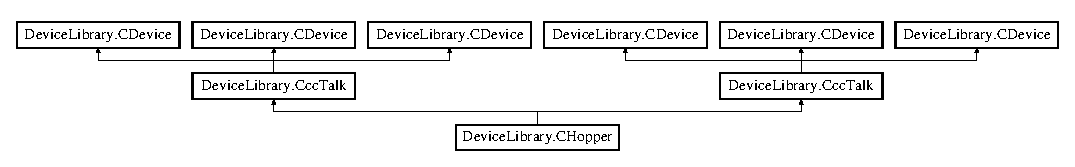
\includegraphics[height=1.794872cm]{class_device_library_1_1_c_hopper}
\end{center}
\end{figure}
\subsection*{Classes}
\begin{DoxyCompactItemize}
\item 
class \mbox{\hyperlink{class_device_library_1_1_c_hopper_1_1_c_empty_count}{C\+Empty\+Count}}
\begin{DoxyCompactList}\small\item\em Class contenant les résultats du vidage du hopper. \end{DoxyCompactList}\item 
class \mbox{\hyperlink{class_device_library_1_1_c_hopper_1_1_c_hopper_coin_id}{C\+Hopper\+Coin\+Id}}
\begin{DoxyCompactList}\small\item\em Identification de la dénomination de la pièce gerée par le hopper \end{DoxyCompactList}\item 
class \mbox{\hyperlink{class_device_library_1_1_c_hopper_1_1_c_hopper_error}{C\+Hopper\+Error}}
\begin{DoxyCompactList}\small\item\em Classe contenant les informations sur une erreur survenue dans le hopper \end{DoxyCompactList}\item 
class \mbox{\hyperlink{class_device_library_1_1_c_hopper_1_1_c_hopper_status}{C\+Hopper\+Status}}
\begin{DoxyCompactList}\small\item\em Classe des status des hoppers \end{DoxyCompactList}\end{DoxyCompactItemize}
\subsection*{Public Types}
\begin{DoxyCompactItemize}
\item 
enum \mbox{\hyperlink{class_device_library_1_1_c_hopper_a5f54d84c3b2a93420c8ff69b1351c77a}{Etat}} \+: byte \{ \newline
\mbox{\hyperlink{class_device_library_1_1_c_hopper_a5f54d84c3b2a93420c8ff69b1351c77aab5859d8721cfdc0312b2838b9c985bc1}{Etat.\+R\+E\+S\+ET}}, 
\mbox{\hyperlink{class_device_library_1_1_c_hopper_a5f54d84c3b2a93420c8ff69b1351c77aaf55af7d8c1565860959f0a29bb0b1c68}{Etat.\+D\+I\+S\+P\+E\+N\+SE}}, 
\mbox{\hyperlink{class_device_library_1_1_c_hopper_a5f54d84c3b2a93420c8ff69b1351c77aa2694f660e3aace318710c802c4026c41}{Etat.\+D\+I\+S\+P\+E\+N\+S\+E\+I\+N\+P\+R\+O\+G\+R\+E\+SS}}, 
\mbox{\hyperlink{class_device_library_1_1_c_hopper_a5f54d84c3b2a93420c8ff69b1351c77aa8116fffa8cbfef37beeb326b739da585}{Etat.\+E\+N\+D\+D\+I\+S\+P\+E\+N\+SE}}, 
\newline
\mbox{\hyperlink{class_device_library_1_1_c_hopper_a5f54d84c3b2a93420c8ff69b1351c77aaa5daf7f2ebbba4975d61dab1c40188c7}{Etat.\+I\+D\+LE}} = 0\+X\+FF
 \}
\begin{DoxyCompactList}\small\item\em Etat de la machine d\textquotesingle{}état des hoppers \end{DoxyCompactList}\item 
enum \mbox{\hyperlink{class_device_library_1_1_c_hopper_afce8f2089a688f1d3fdf9db91242fb01}{Registre\+Pos}} \+: byte \{ \newline
\mbox{\hyperlink{class_device_library_1_1_c_hopper_afce8f2089a688f1d3fdf9db91242fb01a6c3e226b4d4795d518ab341b0824ec29}{Registre\+Pos.\+N\+U\+LL}} = 0, 
\mbox{\hyperlink{class_device_library_1_1_c_hopper_afce8f2089a688f1d3fdf9db91242fb01a2c6dbfb7f793fa40620ac62174479d61}{Registre\+Pos.\+S\+I\+N\+G\+L\+E\+P\+A\+Y\+O\+UT}} = 0\+X02, 
\mbox{\hyperlink{class_device_library_1_1_c_hopper_afce8f2089a688f1d3fdf9db91242fb01a6f836722e3e4f3c3a219159530d2e965}{Registre\+Pos.\+M\+O\+T\+O\+R\+R\+E\+V\+E\+R\+S\+ED}} = 0\+X04, 
\mbox{\hyperlink{class_device_library_1_1_c_hopper_afce8f2089a688f1d3fdf9db91242fb01a055c1a591abb0e8cd86dc969727bcc0b}{Registre\+Pos.\+D\+I\+S\+A\+B\+L\+ED}} = 0\+X80, 
\newline
\mbox{\hyperlink{class_device_library_1_1_c_hopper_afce8f2089a688f1d3fdf9db91242fb01a9cb9d4ef7914bee6cdedcf7524b6d5ef}{Registre\+Pos.\+P\+I\+N\+N\+U\+M\+B\+ER}} = 0\+X80, 
{\bfseries Erreur}, 
\mbox{\hyperlink{class_device_library_1_1_c_hopper_afce8f2089a688f1d3fdf9db91242fb01a352f5cd9841dc6e7e999caee1c876c11}{Registre\+Pos.\+M\+A\+X\+C\+U\+R\+R\+E\+N\+T\+E\+X\+C\+E\+E\+D\+ED}} = 0\+X01, 
\mbox{\hyperlink{class_device_library_1_1_c_hopper_afce8f2089a688f1d3fdf9db91242fb01ad8dffe032a7fbd1f7291f20a1d24fff9}{Registre\+Pos.\+O\+P\+T\+O\+S\+H\+O\+R\+T\+C\+I\+R\+C\+U\+IT}} = 0\+X01, 
\newline
\mbox{\hyperlink{class_device_library_1_1_c_hopper_afce8f2089a688f1d3fdf9db91242fb01a89249c979952ff149dff1f387f78fe0c}{Registre\+Pos.\+T\+O\+O\+C\+C\+U\+R\+ED}} = 0\+X02, 
\mbox{\hyperlink{class_device_library_1_1_c_hopper_afce8f2089a688f1d3fdf9db91242fb01ae24020ff08165f92b4d9649daecd0842}{Registre\+Pos.\+C\+H\+E\+C\+K\+S\+U\+MA}} = 0\+X04, 
\mbox{\hyperlink{class_device_library_1_1_c_hopper_afce8f2089a688f1d3fdf9db91242fb01a84c9b37d0d3499483dae26abd03c62d3}{Registre\+Pos.\+O\+P\+T\+O\+P\+A\+T\+H\+B\+L\+O\+C\+K\+ED}} = 0\+X08, 
\mbox{\hyperlink{class_device_library_1_1_c_hopper_afce8f2089a688f1d3fdf9db91242fb01a61592fb0b332b2fcc7d57d8efade7246}{Registre\+Pos.\+C\+H\+E\+C\+K\+S\+U\+MB}} = 0\+X08, 
\newline
\mbox{\hyperlink{class_device_library_1_1_c_hopper_afce8f2089a688f1d3fdf9db91242fb01aced9f2887aace32933e6db874aa8d6e5}{Registre\+Pos.\+O\+P\+T\+O\+S\+H\+O\+R\+T\+C\+I\+R\+C\+U\+I\+T\+I\+D\+LE}} = 0\+X10, 
\mbox{\hyperlink{class_device_library_1_1_c_hopper_afce8f2089a688f1d3fdf9db91242fb01a18179929e477a9f8fd21d888e8f7a326}{Registre\+Pos.\+C\+H\+E\+C\+K\+S\+U\+MC}} = 0\+X10, 
\mbox{\hyperlink{class_device_library_1_1_c_hopper_afce8f2089a688f1d3fdf9db91242fb01a3597b58c77eec0e7e44fa0f3be8c8e65}{Registre\+Pos.\+O\+P\+T\+O\+B\+L\+O\+C\+K\+E\+D\+P\+E\+R\+M\+A\+N\+E\+N\+T\+LY}} = 0\+X20, 
\mbox{\hyperlink{class_device_library_1_1_c_hopper_afce8f2089a688f1d3fdf9db91242fb01a51a993adb4ff5f07953ff92ac1fa14a9}{Registre\+Pos.\+C\+H\+E\+C\+K\+S\+U\+MD}} = 0\+X20, 
\newline
\mbox{\hyperlink{class_device_library_1_1_c_hopper_afce8f2089a688f1d3fdf9db91242fb01ab3e172b7afeb285bddcec5aee2be298e}{Registre\+Pos.\+P\+O\+W\+E\+R\+UP}} = 0\+X40, 
\mbox{\hyperlink{class_device_library_1_1_c_hopper_afce8f2089a688f1d3fdf9db91242fb01ab77007e73cc2dd997f4ab2846a075e01}{Registre\+Pos.\+P\+O\+W\+E\+R\+F\+A\+IL}} = 0\+X40, 
{\bfseries }
 \}
\item 
enum \mbox{\hyperlink{group___header_gab8e15517b29b9562c7d7e8616d61c855}{Header}} \+: byte \{ \newline
\mbox{\hyperlink{group___header_ggab8e15517b29b9562c7d7e8616d61c855a4825c2517fdde4d526de02666fd27c5c}{Header.\+R\+E\+Q\+U\+E\+S\+T\+H\+I\+G\+H\+L\+O\+W\+S\+T\+A\+T\+US}} = 217, 
\mbox{\hyperlink{group___header_ggab8e15517b29b9562c7d7e8616d61c855a2443533d40c7fd63fffb95385894bf77}{Header.\+M\+O\+D\+I\+F\+Y\+P\+A\+Y\+O\+U\+T\+A\+B\+S\+O\+L\+U\+T\+E\+C\+O\+U\+NT}} = 208, 
\mbox{\hyperlink{group___header_ggab8e15517b29b9562c7d7e8616d61c855aed33fd598b7b9183cf33f46a57889b2a}{Header.\+R\+E\+Q\+U\+E\+S\+T\+P\+A\+Y\+O\+U\+T\+A\+B\+S\+O\+L\+U\+T\+E\+C\+O\+U\+NT}} = 207, 
\mbox{\hyperlink{group___header_ggab8e15517b29b9562c7d7e8616d61c855a7b21bd88ed5c233104fe92303501113c}{Header.\+M\+O\+D\+I\+F\+Y\+P\+A\+Y\+O\+U\+T\+C\+A\+P\+A\+C\+I\+TY}} = 187, 
\newline
\mbox{\hyperlink{group___header_ggab8e15517b29b9562c7d7e8616d61c855a7ba5c462ff3d7dcf46912956b29def0c}{Header.\+R\+E\+Q\+U\+E\+S\+T\+P\+A\+Y\+O\+U\+T\+C\+A\+P\+A\+C\+I\+TY}} = 186, 
\mbox{\hyperlink{group___header_ggab8e15517b29b9562c7d7e8616d61c855ac2ddb98fb918c6472784f387bfc739c0}{Header.\+M\+O\+D\+I\+F\+Y\+P\+A\+Y\+O\+U\+T\+F\+L\+O\+AT}} = 175, 
\mbox{\hyperlink{group___header_ggab8e15517b29b9562c7d7e8616d61c855a86ec4dd896616de2522b741b3ee3c983}{Header.\+R\+E\+Q\+U\+E\+S\+T\+P\+A\+Y\+O\+U\+T\+F\+L\+O\+AT}} = 174, 
\mbox{\hyperlink{group___header_ggab8e15517b29b9562c7d7e8616d61c855afccebf5298d1c1e7db4e5c4ea96a8a76}{Header.\+E\+M\+E\+R\+G\+E\+N\+C\+Y\+S\+T\+OP}} = 172, 
\newline
\mbox{\hyperlink{group___header_ggab8e15517b29b9562c7d7e8616d61c855a2751d29dc0030efbf6bb9434ec9ba968}{Header.\+R\+E\+Q\+U\+E\+S\+T\+H\+O\+P\+P\+E\+R\+C\+O\+IN}} = 171, 
\mbox{\hyperlink{group___header_ggab8e15517b29b9562c7d7e8616d61c855a74205479553e32f9c1896d8eee4ef6bd}{Header.\+R\+E\+Q\+U\+E\+S\+T\+H\+O\+P\+P\+E\+R\+D\+I\+S\+P\+E\+N\+S\+E\+C\+O\+U\+NT}} = 168, 
\mbox{\hyperlink{group___header_ggab8e15517b29b9562c7d7e8616d61c855ab539a90bcfde6ce366c0723b0d0163a8}{Header.\+D\+I\+S\+P\+E\+N\+S\+E\+H\+O\+P\+P\+E\+R\+C\+O\+I\+NS}} = 167, 
\mbox{\hyperlink{group___header_ggab8e15517b29b9562c7d7e8616d61c855ac873dcc3fe0f16c7e169b542a5ce9121}{Header.\+R\+E\+Q\+U\+E\+S\+T\+H\+O\+P\+P\+E\+R\+S\+T\+A\+T\+US}} = 166, 
\newline
\mbox{\hyperlink{group___header_ggab8e15517b29b9562c7d7e8616d61c855ae924a1d3fed578124d2542b501b9d5be}{Header.\+M\+O\+D\+I\+F\+Y\+V\+A\+R\+I\+A\+B\+L\+E\+S\+ET}} = 165, 
\mbox{\hyperlink{group___header_ggab8e15517b29b9562c7d7e8616d61c855a1c7e15da01d0f3d0d6c3699f4428ae19}{Header.\+E\+N\+A\+B\+L\+E\+H\+O\+P\+P\+ER}} = 164, 
\mbox{\hyperlink{group___header_ggab8e15517b29b9562c7d7e8616d61c855a94aba60ee791b51c24268564d6d4db34}{Header.\+T\+E\+S\+T\+H\+O\+P\+P\+ER}} = 163, 
\mbox{\hyperlink{group___header_ggab8e15517b29b9562c7d7e8616d61c855ab3b80d8e35f9bf8fd78fbb4ebf2e065d}{Header.\+P\+U\+M\+P\+R\+NG}} = 161, 
\newline
\mbox{\hyperlink{group___header_ggab8e15517b29b9562c7d7e8616d61c855aaa3f8f4acd8572ce7e9f4fe87954b6c0}{Header.\+R\+E\+Q\+U\+E\+S\+T\+C\+I\+P\+H\+E\+R\+K\+EY}} = 160, 
\mbox{\hyperlink{group___header_ggab8e15517b29b9562c7d7e8616d61c855a3f0803c91adce917551e3653ce6ab02b}{Header.\+D\+I\+S\+P\+E\+N\+S\+E\+H\+O\+P\+P\+E\+R\+V\+A\+L\+UE}} = 134, 
\mbox{\hyperlink{group___header_ggab8e15517b29b9562c7d7e8616d61c855af4cf967e4b4c084bb9148099781b3a49}{Header.\+R\+E\+Q\+U\+E\+S\+T\+H\+O\+P\+P\+E\+R\+P\+O\+L\+L\+I\+N\+G\+V\+A\+L\+UE}} = 133, 
\mbox{\hyperlink{group___header_ggab8e15517b29b9562c7d7e8616d61c855ab7f6a886cf52347442b934ad59273c7d}{Header.\+E\+M\+E\+R\+G\+E\+N\+C\+Y\+S\+T\+O\+P\+V\+A\+L\+UE}} = 132, 
\newline
\mbox{\hyperlink{group___header_ggab8e15517b29b9562c7d7e8616d61c855a6ad8e7feb8e305d7b549b257c70d3ddf}{Header.\+R\+E\+Q\+U\+E\+S\+T\+H\+O\+P\+P\+E\+R\+C\+O\+I\+N\+V\+A\+L\+UE}} = 131, 
\mbox{\hyperlink{group___header_ggab8e15517b29b9562c7d7e8616d61c855a954b2d7e92fb3c676e4246f551a03871}{Header.\+R\+E\+Q\+U\+E\+S\+T\+I\+N\+D\+E\+X\+E\+D\+D\+H\+O\+P\+P\+E\+R\+D\+I\+S\+P\+E\+N\+S\+E\+C\+O\+U\+NT}} = 130, 
\mbox{\hyperlink{group___header_ggab8e15517b29b9562c7d7e8616d61c855aa0d004c8327a3e8b0ae5165246991c25}{Header.\+R\+E\+Q\+U\+E\+S\+T\+E\+N\+C\+R\+Y\+P\+T\+E\+D\+H\+O\+P\+P\+E\+R\+S\+T\+A\+T\+US}} = 109
 \}
\begin{DoxyCompactList}\small\item\em Liste des commandes cc\+Talk spécifiques aux hoppers \end{DoxyCompactList}\end{DoxyCompactItemize}
\subsection*{Public Member Functions}
\begin{DoxyCompactItemize}
\item 
\mbox{\hyperlink{class_device_library_1_1_c_hopper_a25c0ba824eb783ecdec6c6f53f90f243}{C\+Hopper}} (byte hopper\+Number)
\begin{DoxyCompactList}\small\item\em Constructeur \end{DoxyCompactList}\item 
int \mbox{\hyperlink{class_device_library_1_1_c_hopper_a6c3cbf56cd236d0867a96e5345f6b881}{Get\+Resetable\+Counter}} ()
\begin{DoxyCompactList}\small\item\em Lit les informations du compteur interne du hopper \end{DoxyCompactList}\item 
void \mbox{\hyperlink{class_device_library_1_1_c_hopper_ad4e3e04686c9cabd002597ebd8fa3712}{Pump\+R\+NG}} ()
\begin{DoxyCompactList}\small\item\em Envoie un nombre aléatoire qui sera utilisé pour le chiffrement. \end{DoxyCompactList}\item 
bool \mbox{\hyperlink{class_device_library_1_1_c_hopper_adc0fd478490e3ef5e255f7bc2f64f506}{Dispense\+Coins}} (byte number)
\begin{DoxyCompactList}\small\item\em Commande demandant la distribution des pièces. \end{DoxyCompactList}\item 
void \mbox{\hyperlink{class_device_library_1_1_c_hopper_aa47c51849127934ffa8b0fd19a46344a}{Init}} ()
\begin{DoxyCompactList}\small\item\em Initialisation du hopper \end{DoxyCompactList}\item 
void \mbox{\hyperlink{class_device_library_1_1_c_hopper_aa46a9adf83ee5e25c9d6c6f3e315501a}{Check\+Level}} (object state=null)
\begin{DoxyCompactList}\small\item\em Véfication des niveaux du hopper. \end{DoxyCompactList}\item 
void \mbox{\hyperlink{class_device_library_1_1_c_hopper_ae47327ae35305769239ffd9922081d57}{Empty}} ()
\begin{DoxyCompactList}\small\item\em Demande le vidage du hopper; \end{DoxyCompactList}\item 
void \mbox{\hyperlink{class_device_library_1_1_c_hopper_a43760bb1d6cac2e875eb6ddb7615a90a}{Check\+State}} ()
\begin{DoxyCompactList}\small\item\em Polling de la machine d\textquotesingle{}état des hoppers. \end{DoxyCompactList}\item 
override string \mbox{\hyperlink{class_device_library_1_1_c_hopper_a25b43f1aafc2b92432077743ce07b39c}{To\+String}} ()
\begin{DoxyCompactList}\small\item\em Ìdentification du hopper. \end{DoxyCompactList}\item 
void \mbox{\hyperlink{class_device_library_1_1_c_hopper_a1161f40b938189953cede1eb8a844672}{Distribute}} (byte number\+To\+Dispense)
\begin{DoxyCompactList}\small\item\em Provoque la distribution par le hopper en utilisant la machine d\textquotesingle{}état \end{DoxyCompactList}\item 
void \mbox{\hyperlink{class_device_library_1_1_c_hopper_a2fa0700c53416b25e7cad3dd626a1753}{Sub\+Counters}} (long Coins\+Number)
\begin{DoxyCompactList}\small\item\em Mise à jour des compteurs après une distribution. \end{DoxyCompactList}\item 
void \mbox{\hyperlink{class_device_library_1_1_c_hopper_aa36d7fe76437086718eee22bc8189d3b}{Load\+Hopper}} (long Coins\+Number)
\begin{DoxyCompactList}\small\item\em Recharge les compteurs du hopper \end{DoxyCompactList}\item 
void \mbox{\hyperlink{class_device_library_1_1_c_hopper_a254a7cbf891dec96caf087ab56512bc8}{Task\+Hopper}} ()
\begin{DoxyCompactList}\small\item\em Tâche de la machine d\textquotesingle{}état du hopper. \end{DoxyCompactList}\end{DoxyCompactItemize}
\subsection*{Public Attributes}
\begin{DoxyCompactItemize}
\item 
const byte \mbox{\hyperlink{class_device_library_1_1_c_hopper_a109908437c130d0e5f081f13ab48c98c}{max\+Hopper}} = 8
\begin{DoxyCompactList}\small\item\em Nombre maximum de hoppers \end{DoxyCompactList}\item 
\mbox{\hyperlink{class_device_library_1_1_c_hopper_1_1_c_hopper_error}{C\+Hopper\+Error}} \mbox{\hyperlink{class_device_library_1_1_c_hopper_ad9d867e3315d21fea58b64b696fa8d17}{error\+Hopper}}
\begin{DoxyCompactList}\small\item\em Instance de la class Cerror\+Hopper \end{DoxyCompactList}\item 
bool \mbox{\hyperlink{class_device_library_1_1_c_hopper_a2489ae3898da396040859ec4c86bd3e0}{is\+Hopper\+Error}}
\begin{DoxyCompactList}\small\item\em Indique la présence d\textquotesingle{}une erreur sur le hopper \end{DoxyCompactList}\item 
bool \mbox{\hyperlink{class_device_library_1_1_c_hopper_aa78b1d599715ada39ff0a032db1703a0}{is\+Emptying\+In\+Progress}}
\begin{DoxyCompactList}\small\item\em Flag indiquant qu\textquotesingle{}un vidage est en cours. \end{DoxyCompactList}\item 
bool \mbox{\hyperlink{class_device_library_1_1_c_hopper_a13463c888437b418637de1d7e2cd4231}{is\+Emptied}}
\begin{DoxyCompactList}\small\item\em Indique si le hopper a été vidé \end{DoxyCompactList}\item 
const byte \mbox{\hyperlink{class_device_library_1_1_c_hopper_a8d069f368b3dd2356d76b8244181168b}{Address\+Base\+Hoper}} = 2
\begin{DoxyCompactList}\small\item\em Adresse de base des hoppers. \end{DoxyCompactList}\item 
\mbox{\hyperlink{class_device_library_1_1_c_hopper_variable_set}{C\+Hopper\+Variable\+Set}} \mbox{\hyperlink{class_device_library_1_1_c_hopper_ab4e4002ee1d9863f6eaf3e67526d4c9a}{variables}}
\begin{DoxyCompactList}\small\item\em Objet contenant l\textquotesingle{}ensemble des variables du hopper \end{DoxyCompactList}\item 
\mbox{\hyperlink{class_device_library_1_1_c_hopper_1_1_c_hopper_status}{C\+Hopper\+Status}} \mbox{\hyperlink{class_device_library_1_1_c_hopper_ab1706fc6c299ceacbbc2d16a11229f41}{dispense\+Status}}
\begin{DoxyCompactList}\small\item\em Objet contenant le status de la distribution en cours. \end{DoxyCompactList}\item 
byte \mbox{\hyperlink{class_device_library_1_1_c_hopper_af41c804396bf26e0d2275a1d90f763e2}{Number}}
\begin{DoxyCompactList}\small\item\em Numéro d\textquotesingle{}ordre du hopper \end{DoxyCompactList}\item 
\mbox{\hyperlink{class_device_library_1_1_c_memory_storage}{C\+Memory\+Storage}} \mbox{\hyperlink{class_device_library_1_1_c_hopper_a3896efcc3ac63f3c01d3871d8f74881d}{memory\+Storage}}
\begin{DoxyCompactList}\small\item\em Informations sur le maintien des donneés en mémoires \end{DoxyCompactList}\item 
\mbox{\hyperlink{class_device_library_1_1_c_hopper_1_1_c_empty_count}{C\+Empty\+Count}} \mbox{\hyperlink{class_device_library_1_1_c_hopper_aa38216ffa60bf350c59c59af0de3fa7b}{empty\+Count}}
\begin{DoxyCompactList}\small\item\em Compteur de vidage; \end{DoxyCompactList}\item 
Thread \mbox{\hyperlink{class_device_library_1_1_c_hopper_acfcffc972c7e842f7bf34140fd320a27}{H\+Task}}
\begin{DoxyCompactList}\small\item\em Thread de la machine d\textquotesingle{}état du hopper. \end{DoxyCompactList}\end{DoxyCompactItemize}
\subsection*{Properties}
\begin{DoxyCompactItemize}
\item 
uint \mbox{\hyperlink{class_device_library_1_1_c_hopper_a78903783271cadf2c222e983c46009f5}{Coin\+Value}}\hspace{0.3cm}{\ttfamily  \mbox{[}get, set\mbox{]}}
\begin{DoxyCompactList}\small\item\em Valeur de la pièce distribuée par le hopper. \end{DoxyCompactList}\item 
long \mbox{\hyperlink{class_device_library_1_1_c_hopper_a3c755d041eabd52ba997d42822658f91}{Coins\+In\+Hopper}}\hspace{0.3cm}{\ttfamily  \mbox{[}get, set\mbox{]}}
\begin{DoxyCompactList}\small\item\em Compteur du nombre de pièce dans le hopper \end{DoxyCompactList}\item 
long \mbox{\hyperlink{class_device_library_1_1_c_hopper_a0a7c83ec2bf3e3ac22e6585e6c0ff4ae}{Amount\+In\+Hopper}}\hspace{0.3cm}{\ttfamily  \mbox{[}get, set\mbox{]}}
\begin{DoxyCompactList}\small\item\em Montant contenu dans le hopper. \end{DoxyCompactList}\item 
long \mbox{\hyperlink{class_device_library_1_1_c_hopper_ab6a5f0c6c2bfb253f65d75d0f7006e5f}{Coins\+Out}}\hspace{0.3cm}{\ttfamily  \mbox{[}get, set\mbox{]}}
\begin{DoxyCompactList}\small\item\em Compteur de pièces distribuées \end{DoxyCompactList}\item 
long \mbox{\hyperlink{class_device_library_1_1_c_hopper_a341c4cee94631414e512d7edf2d3b2fc}{Amount\+Out}}\hspace{0.3cm}{\ttfamily  \mbox{[}get, set\mbox{]}}
\begin{DoxyCompactList}\small\item\em Montant distribués \end{DoxyCompactList}\item 
long \mbox{\hyperlink{class_device_library_1_1_c_hopper_a5ace9c8caf38ba82416201a92908d426}{Coins\+Loaded\+In\+Hopper}}\hspace{0.3cm}{\ttfamily  \mbox{[}get, set\mbox{]}}
\begin{DoxyCompactList}\small\item\em Nombre de pièces chargées dans le hopper \end{DoxyCompactList}\item 
long \mbox{\hyperlink{class_device_library_1_1_c_hopper_a9a68e629bcbc3cfc2c6828516e2a152d}{Amount\+Loaded\+In\+Hopper}}\hspace{0.3cm}{\ttfamily  \mbox{[}get, set\mbox{]}}
\begin{DoxyCompactList}\small\item\em Montant chargé dans le hopper. \end{DoxyCompactList}\item 
\mbox{\hyperlink{class_device_library_1_1_c_hopper_a5f54d84c3b2a93420c8ff69b1351c77a}{Etat}} \mbox{\hyperlink{class_device_library_1_1_c_hopper_aa9f1e8689d187df5894527e7c02dc875}{State}}\hspace{0.3cm}{\ttfamily  \mbox{[}get, set\mbox{]}}
\begin{DoxyCompactList}\small\item\em Etat de la machine d\textquotesingle{}état des hoppers \end{DoxyCompactList}\item 
bool \mbox{\hyperlink{class_device_library_1_1_c_hopper_a045b85a17c558f578649aca5d387561b}{Is\+Max\+Current\+Exceeded}}\hspace{0.3cm}{\ttfamily  \mbox{[}get\mbox{]}}
\begin{DoxyCompactList}\small\item\em Bolean indiquant qu\textquotesingle{}un dépassement du courant maximun a été atteint. \end{DoxyCompactList}\item 
bool \mbox{\hyperlink{class_device_library_1_1_c_hopper_adf2e0f18bd630e28e89aea2f45ef6a19}{Is\+T\+O\+Occured}}\hspace{0.3cm}{\ttfamily  \mbox{[}get\mbox{]}}
\begin{DoxyCompactList}\small\item\em Bolean indiquant qu\textquotesingle{}un dépassement du temps alloué pour l\textquotesingle{}éjection d\textquotesingle{}une pièce est survenu. \end{DoxyCompactList}\item 
bool \mbox{\hyperlink{class_device_library_1_1_c_hopper_a9e9bbbee8c2ec524e36442a66482d41f}{Is\+Motor\+Reversed}}\hspace{0.3cm}{\ttfamily  \mbox{[}get\mbox{]}}
\begin{DoxyCompactList}\small\item\em Bolean indiquant que suite à une surconsomation la rotation du moteur a été inversée pour corriger un bourrage. \end{DoxyCompactList}\item 
bool \mbox{\hyperlink{class_device_library_1_1_c_hopper_aba941b8ab4317792660483f287171363}{Is\+Opto\+Path\+Blocked}}\hspace{0.3cm}{\ttfamily  \mbox{[}get\mbox{]}}
\begin{DoxyCompactList}\small\item\em Bolean indiquant que la sortie est bloquée. \end{DoxyCompactList}\item 
bool \mbox{\hyperlink{class_device_library_1_1_c_hopper_aa52f0af92ae272576ec14a79c6356e96}{Is\+Short\+Circuit}}\hspace{0.3cm}{\ttfamily  \mbox{[}get\mbox{]}}
\begin{DoxyCompactList}\small\item\em Bolean indiquant que la sortie est en court-\/circuit. \end{DoxyCompactList}\item 
bool \mbox{\hyperlink{class_device_library_1_1_c_hopper_ad7168dd39fa5f937164d357c3236321d}{Is\+Opto\+Permanently\+Blocked}}\hspace{0.3cm}{\ttfamily  \mbox{[}get\mbox{]}}
\begin{DoxyCompactList}\small\item\em Bolean indiquant qu\textquotesingle{}un optocloupleur est bloqué en permanence. \end{DoxyCompactList}\item 
bool \mbox{\hyperlink{class_device_library_1_1_c_hopper_a5a9d29bab15e199a614d991b6b860c5a}{Is\+Power\+Up\+Detected}}\hspace{0.3cm}{\ttfamily  \mbox{[}get\mbox{]}}
\begin{DoxyCompactList}\small\item\em Bolean indiquant que le hopper est alimenté et un reset n\textquotesingle{}est pas encore effectué \end{DoxyCompactList}\item 
bool \mbox{\hyperlink{class_device_library_1_1_c_hopper_a5f728eaab6f916a56b0927cfef1c836f}{Is\+Payout\+Disabled}}\hspace{0.3cm}{\ttfamily  \mbox{[}get\mbox{]}}
\begin{DoxyCompactList}\small\item\em Bolean indiquant que le hopper n\textquotesingle{}est pas activé \end{DoxyCompactList}\item 
bool \mbox{\hyperlink{class_device_library_1_1_c_hopper_afca797bea58cb663b8b3784df7c9dc65}{Is\+Opto\+Shor\+Circuit}}\hspace{0.3cm}{\ttfamily  \mbox{[}get\mbox{]}}
\begin{DoxyCompactList}\small\item\em Bolean indiquant qu\textquotesingle{}un optocoupleur est en court-\/circuit \end{DoxyCompactList}\item 
bool \mbox{\hyperlink{class_device_library_1_1_c_hopper_ac8bdea555bab297e4533885935005ad9}{Is\+Single\+Coin\+Mode}}\hspace{0.3cm}{\ttfamily  \mbox{[}get\mbox{]}}
\begin{DoxyCompactList}\small\item\em Bolean indiquant que le hopper est en mode pièce par pièce. \end{DoxyCompactList}\item 
bool \mbox{\hyperlink{class_device_library_1_1_c_hopper_ab6b53cde806c99f06e7ab4e51044c68c}{Is\+Check\+Sum\+A\+Error}}\hspace{0.3cm}{\ttfamily  \mbox{[}get\mbox{]}}
\begin{DoxyCompactList}\small\item\em Bolean indiquant qu\textquotesingle{}une erreur de checksum dans le bloc de données A est survenue. \end{DoxyCompactList}\item 
bool \mbox{\hyperlink{class_device_library_1_1_c_hopper_a97fc7f01be900cd25941c1cc0d1ff053}{Is\+Check\+Sum\+B\+Error}}\hspace{0.3cm}{\ttfamily  \mbox{[}get\mbox{]}}
\begin{DoxyCompactList}\small\item\em Bolean indiquant qu\textquotesingle{}une erreur de checksum dans le bloc de données B est survenue. \end{DoxyCompactList}\item 
bool \mbox{\hyperlink{class_device_library_1_1_c_hopper_abcd01eec19d5cefaaf8f7a8a748777c1}{Is\+Check\+Sum\+C\+Error}}\hspace{0.3cm}{\ttfamily  \mbox{[}get\mbox{]}}
\begin{DoxyCompactList}\small\item\em Bolean indiquant qu\textquotesingle{}une erreur de checksum dans le bloc de données B est survenue. \end{DoxyCompactList}\item 
bool \mbox{\hyperlink{class_device_library_1_1_c_hopper_af21105cacff9feef51796a71f1066d6c}{Is\+Check\+Sum\+D\+Error}}\hspace{0.3cm}{\ttfamily  \mbox{[}get\mbox{]}}
\begin{DoxyCompactList}\small\item\em Bolean indiquant qu\textquotesingle{}une erreur de checksum dans le bloc de données D est survenue. \end{DoxyCompactList}\item 
bool \mbox{\hyperlink{class_device_library_1_1_c_hopper_ab6ddbdf218466891ec4df5b618f22b57}{Is\+Power\+Fail\+Memory\+Write}}\hspace{0.3cm}{\ttfamily  \mbox{[}get\mbox{]}}
\begin{DoxyCompactList}\small\item\em Bolean indiquant qu\textquotesingle{}une chute de tension a eu lieu pendant une écriture mémoire. \end{DoxyCompactList}\item 
bool \mbox{\hyperlink{class_device_library_1_1_c_hopper_a6cba5628502ed179dc886abe0e553879}{Is\+P\+I\+N\+Enabled}}\hspace{0.3cm}{\ttfamily  \mbox{[}get\mbox{]}}
\begin{DoxyCompactList}\small\item\em Bolean indiquant qu\textquotesingle{}un code pin est utilisé par le hopper \end{DoxyCompactList}\item 
byte \mbox{\hyperlink{class_device_library_1_1_c_hopper_a11dafc48a8a680909486f10a61b80de1}{Coins\+To\+Distribute}}\hspace{0.3cm}{\ttfamily  \mbox{[}get, set\mbox{]}}
\begin{DoxyCompactList}\small\item\em Nombre de pièce à distribuer \end{DoxyCompactList}\item 
uint \mbox{\hyperlink{class_device_library_1_1_c_hopper_ade03b189fd3b60ae0be1b0ecc4b58177}{Level\+Full\+Soft}}\hspace{0.3cm}{\ttfamily  \mbox{[}get, set\mbox{]}}
\begin{DoxyCompactList}\small\item\em Nombre maximum de pièces autorisées \end{DoxyCompactList}\item 
uint \mbox{\hyperlink{class_device_library_1_1_c_hopper_add0b0bb819e03109708b70ceecc31106}{Level\+H\+I\+Soft}}\hspace{0.3cm}{\ttfamily  \mbox{[}get, set\mbox{]}}
\begin{DoxyCompactList}\small\item\em Nombre de pièce pour le niveau d\textquotesingle{}alerte haut \end{DoxyCompactList}\item 
uint \mbox{\hyperlink{class_device_library_1_1_c_hopper_a27713aed4b5a8f43ec2998ddec6ad5f2}{Level\+L\+O\+Soft}}\hspace{0.3cm}{\ttfamily  \mbox{[}get, set\mbox{]}}
\begin{DoxyCompactList}\small\item\em Nombre de pièce pour le niveau d\textquotesingle{}alerte bas \end{DoxyCompactList}\item 
uint \mbox{\hyperlink{class_device_library_1_1_c_hopper_aa319784d7be6861029637485981d5bc8}{Level\+Empty\+Soft}}\hspace{0.3cm}{\ttfamily  \mbox{[}get, set\mbox{]}}
\begin{DoxyCompactList}\small\item\em Nombre minimum de pièces autorisées \end{DoxyCompactList}\item 
uint \mbox{\hyperlink{class_device_library_1_1_c_hopper_ad75b00a2bcc10f3340ffb6b3735bea7a}{Default\+Filling}}\hspace{0.3cm}{\ttfamily  \mbox{[}get, set\mbox{]}}
\begin{DoxyCompactList}\small\item\em Nombre de pièces par défaut pour un remplissage. \end{DoxyCompactList}\item 
bool \mbox{\hyperlink{class_device_library_1_1_c_hopper_a1cb25d14b95a28dcd510b354b784a4ab}{Is\+Dispensed}}\hspace{0.3cm}{\ttfamily  \mbox{[}get, set\mbox{]}}
\begin{DoxyCompactList}\small\item\em Boolean indiquant la fin d\textquotesingle{}une distribution \end{DoxyCompactList}\item 
bool \mbox{\hyperlink{class_device_library_1_1_c_hopper_a08a82f43af4ac242d87e2a73734d9159}{Is\+Critical}}\hspace{0.3cm}{\ttfamily  \mbox{[}get, set\mbox{]}}
\begin{DoxyCompactList}\small\item\em Boolean indiquant si le hopper est indispensable au fonctionnement de la borne. \end{DoxyCompactList}\item 
bool \mbox{\hyperlink{class_device_library_1_1_c_hopper_a621e84f9419e3b7fd1c35f3f0a336a31}{Is\+High\+Level\+Implemented}}\hspace{0.3cm}{\ttfamily  \mbox{[}get\mbox{]}}
\begin{DoxyCompactList}\small\item\em Boolean indiquant si la détection du niveau haut est implémentée. \end{DoxyCompactList}\item 
bool \mbox{\hyperlink{class_device_library_1_1_c_hopper_a15324622637cfb57c9a24f321d55a496}{Is\+Low\+Level\+Implemented}}\hspace{0.3cm}{\ttfamily  \mbox{[}get\mbox{]}}
\begin{DoxyCompactList}\small\item\em Indique si la détection du niveau haut est implémentée. \end{DoxyCompactList}\item 
bool \mbox{\hyperlink{class_device_library_1_1_c_hopper_a4f4d3bcff66d7377ab203313ab1778f8}{Is\+High\+Level\+Reached}}\hspace{0.3cm}{\ttfamily  \mbox{[}get\mbox{]}}
\begin{DoxyCompactList}\small\item\em Boolean indiquant si le niveau hardware haut est atteint \end{DoxyCompactList}\item 
bool \mbox{\hyperlink{class_device_library_1_1_c_hopper_a04e41e117c79e3ac0c3cd3dc38d3931e}{Is\+Low\+Level\+Reached}}\hspace{0.3cm}{\ttfamily  \mbox{[}get\mbox{]}}
\begin{DoxyCompactList}\small\item\em Boolean indiquant si le niveau hardware bas est atteint \end{DoxyCompactList}\item 
byte \mbox{\hyperlink{class_device_library_1_1_c_hopper_a1a49cc5d1094fa17df2b465c2c53f658}{Emergecy\+Stop}}\hspace{0.3cm}{\ttfamily  \mbox{[}get\mbox{]}}
\begin{DoxyCompactList}\small\item\em Nombre de byte restant à payer lorsque l\textquotesingle{}arrêt d\textquotesingle{}urgence du hopper est activé. \end{DoxyCompactList}\item 
\mbox{\hyperlink{class_device_library_1_1_c_hopper_1_1_c_hopper_coin_id}{C\+Hopper\+Coin\+Id}} \mbox{\hyperlink{class_device_library_1_1_c_hopper_ac3540ffaafc86345d05281840157f5ad}{Coin\+Id}}\hspace{0.3cm}{\ttfamily  \mbox{[}get\mbox{]}}
\begin{DoxyCompactList}\small\item\em Lecture des informations concernant la pièce gérée par le hopper \end{DoxyCompactList}\end{DoxyCompactItemize}
\subsection*{Additional Inherited Members}


\subsection{Detailed Description}
Classe des hoppers 



\subsection{Member Enumeration Documentation}
\mbox{\Hypertarget{class_device_library_1_1_c_hopper_a5f54d84c3b2a93420c8ff69b1351c77a}\label{class_device_library_1_1_c_hopper_a5f54d84c3b2a93420c8ff69b1351c77a}} 
\index{Device\+Library\+::\+C\+Hopper@{Device\+Library\+::\+C\+Hopper}!Etat@{Etat}}
\index{Etat@{Etat}!Device\+Library\+::\+C\+Hopper@{Device\+Library\+::\+C\+Hopper}}
\subsubsection{\texorpdfstring{Etat}{Etat}}
{\footnotesize\ttfamily enum \mbox{\hyperlink{class_device_library_1_1_c_hopper_a5f54d84c3b2a93420c8ff69b1351c77a}{Device\+Library.\+C\+Hopper.\+Etat}} \+: byte\hspace{0.3cm}{\ttfamily [strong]}}



Etat de la machine d\textquotesingle{}état des hoppers 

\begin{DoxyEnumFields}{Enumerator}
\raisebox{\heightof{T}}[0pt][0pt]{\index{R\+E\+S\+ET@{R\+E\+S\+ET}!Device\+Library\+::\+C\+Hopper@{Device\+Library\+::\+C\+Hopper}}\index{Device\+Library\+::\+C\+Hopper@{Device\+Library\+::\+C\+Hopper}!R\+E\+S\+ET@{R\+E\+S\+ET}}}\mbox{\Hypertarget{class_device_library_1_1_c_hopper_a5f54d84c3b2a93420c8ff69b1351c77aab5859d8721cfdc0312b2838b9c985bc1}\label{class_device_library_1_1_c_hopper_a5f54d84c3b2a93420c8ff69b1351c77aab5859d8721cfdc0312b2838b9c985bc1}} 
R\+E\+S\+ET&Etat initial \\
\hline

\raisebox{\heightof{T}}[0pt][0pt]{\index{D\+I\+S\+P\+E\+N\+SE@{D\+I\+S\+P\+E\+N\+SE}!Device\+Library\+::\+C\+Hopper@{Device\+Library\+::\+C\+Hopper}}\index{Device\+Library\+::\+C\+Hopper@{Device\+Library\+::\+C\+Hopper}!D\+I\+S\+P\+E\+N\+SE@{D\+I\+S\+P\+E\+N\+SE}}}\mbox{\Hypertarget{class_device_library_1_1_c_hopper_a5f54d84c3b2a93420c8ff69b1351c77aaf55af7d8c1565860959f0a29bb0b1c68}\label{class_device_library_1_1_c_hopper_a5f54d84c3b2a93420c8ff69b1351c77aaf55af7d8c1565860959f0a29bb0b1c68}} 
D\+I\+S\+P\+E\+N\+SE&Traitement d\textquotesingle{}une demande de distribution \\
\hline

\raisebox{\heightof{T}}[0pt][0pt]{\index{D\+I\+S\+P\+E\+N\+S\+E\+I\+N\+P\+R\+O\+G\+R\+E\+SS@{D\+I\+S\+P\+E\+N\+S\+E\+I\+N\+P\+R\+O\+G\+R\+E\+SS}!Device\+Library\+::\+C\+Hopper@{Device\+Library\+::\+C\+Hopper}}\index{Device\+Library\+::\+C\+Hopper@{Device\+Library\+::\+C\+Hopper}!D\+I\+S\+P\+E\+N\+S\+E\+I\+N\+P\+R\+O\+G\+R\+E\+SS@{D\+I\+S\+P\+E\+N\+S\+E\+I\+N\+P\+R\+O\+G\+R\+E\+SS}}}\mbox{\Hypertarget{class_device_library_1_1_c_hopper_a5f54d84c3b2a93420c8ff69b1351c77aa2694f660e3aace318710c802c4026c41}\label{class_device_library_1_1_c_hopper_a5f54d84c3b2a93420c8ff69b1351c77aa2694f660e3aace318710c802c4026c41}} 
D\+I\+S\+P\+E\+N\+S\+E\+I\+N\+P\+R\+O\+G\+R\+E\+SS&Distribution en cours \\
\hline

\raisebox{\heightof{T}}[0pt][0pt]{\index{E\+N\+D\+D\+I\+S\+P\+E\+N\+SE@{E\+N\+D\+D\+I\+S\+P\+E\+N\+SE}!Device\+Library\+::\+C\+Hopper@{Device\+Library\+::\+C\+Hopper}}\index{Device\+Library\+::\+C\+Hopper@{Device\+Library\+::\+C\+Hopper}!E\+N\+D\+D\+I\+S\+P\+E\+N\+SE@{E\+N\+D\+D\+I\+S\+P\+E\+N\+SE}}}\mbox{\Hypertarget{class_device_library_1_1_c_hopper_a5f54d84c3b2a93420c8ff69b1351c77aa8116fffa8cbfef37beeb326b739da585}\label{class_device_library_1_1_c_hopper_a5f54d84c3b2a93420c8ff69b1351c77aa8116fffa8cbfef37beeb326b739da585}} 
E\+N\+D\+D\+I\+S\+P\+E\+N\+SE&Traitement fin de distribution \\
\hline

\raisebox{\heightof{T}}[0pt][0pt]{\index{I\+D\+LE@{I\+D\+LE}!Device\+Library\+::\+C\+Hopper@{Device\+Library\+::\+C\+Hopper}}\index{Device\+Library\+::\+C\+Hopper@{Device\+Library\+::\+C\+Hopper}!I\+D\+LE@{I\+D\+LE}}}\mbox{\Hypertarget{class_device_library_1_1_c_hopper_a5f54d84c3b2a93420c8ff69b1351c77aaa5daf7f2ebbba4975d61dab1c40188c7}\label{class_device_library_1_1_c_hopper_a5f54d84c3b2a93420c8ff69b1351c77aaa5daf7f2ebbba4975d61dab1c40188c7}} 
I\+D\+LE&Inactif \\
\hline

\end{DoxyEnumFields}
\mbox{\Hypertarget{class_device_library_1_1_c_hopper_afce8f2089a688f1d3fdf9db91242fb01}\label{class_device_library_1_1_c_hopper_afce8f2089a688f1d3fdf9db91242fb01}} 
\index{Device\+Library\+::\+C\+Hopper@{Device\+Library\+::\+C\+Hopper}!Registre\+Pos@{Registre\+Pos}}
\index{Registre\+Pos@{Registre\+Pos}!Device\+Library\+::\+C\+Hopper@{Device\+Library\+::\+C\+Hopper}}
\subsubsection{\texorpdfstring{Registre\+Pos}{RegistrePos}}
{\footnotesize\ttfamily enum \mbox{\hyperlink{class_device_library_1_1_c_hopper_afce8f2089a688f1d3fdf9db91242fb01}{Device\+Library.\+C\+Hopper.\+Registre\+Pos}} \+: byte\hspace{0.3cm}{\ttfamily [strong]}}





\begin{DoxyEnumFields}{Enumerator}
\raisebox{\heightof{T}}[0pt][0pt]{\index{N\+U\+LL@{N\+U\+LL}!Device\+Library\+::\+C\+Hopper@{Device\+Library\+::\+C\+Hopper}}\index{Device\+Library\+::\+C\+Hopper@{Device\+Library\+::\+C\+Hopper}!N\+U\+LL@{N\+U\+LL}}}\mbox{\Hypertarget{class_device_library_1_1_c_hopper_afce8f2089a688f1d3fdf9db91242fb01a6c3e226b4d4795d518ab341b0824ec29}\label{class_device_library_1_1_c_hopper_afce8f2089a688f1d3fdf9db91242fb01a6c3e226b4d4795d518ab341b0824ec29}} 
N\+U\+LL&summary$>$ Pas d\textquotesingle{}erreur. /summary$>$ \\
\hline

\raisebox{\heightof{T}}[0pt][0pt]{\index{S\+I\+N\+G\+L\+E\+P\+A\+Y\+O\+UT@{S\+I\+N\+G\+L\+E\+P\+A\+Y\+O\+UT}!Device\+Library\+::\+C\+Hopper@{Device\+Library\+::\+C\+Hopper}}\index{Device\+Library\+::\+C\+Hopper@{Device\+Library\+::\+C\+Hopper}!S\+I\+N\+G\+L\+E\+P\+A\+Y\+O\+UT@{S\+I\+N\+G\+L\+E\+P\+A\+Y\+O\+UT}}}\mbox{\Hypertarget{class_device_library_1_1_c_hopper_afce8f2089a688f1d3fdf9db91242fb01a2c6dbfb7f793fa40620ac62174479d61}\label{class_device_library_1_1_c_hopper_afce8f2089a688f1d3fdf9db91242fb01a2c6dbfb7f793fa40620ac62174479d61}} 
S\+I\+N\+G\+L\+E\+P\+A\+Y\+O\+UT&Le pièce par pièce est activé. \\
\hline

\raisebox{\heightof{T}}[0pt][0pt]{\index{M\+O\+T\+O\+R\+R\+E\+V\+E\+R\+S\+ED@{M\+O\+T\+O\+R\+R\+E\+V\+E\+R\+S\+ED}!Device\+Library\+::\+C\+Hopper@{Device\+Library\+::\+C\+Hopper}}\index{Device\+Library\+::\+C\+Hopper@{Device\+Library\+::\+C\+Hopper}!M\+O\+T\+O\+R\+R\+E\+V\+E\+R\+S\+ED@{M\+O\+T\+O\+R\+R\+E\+V\+E\+R\+S\+ED}}}\mbox{\Hypertarget{class_device_library_1_1_c_hopper_afce8f2089a688f1d3fdf9db91242fb01a6f836722e3e4f3c3a219159530d2e965}\label{class_device_library_1_1_c_hopper_afce8f2089a688f1d3fdf9db91242fb01a6f836722e3e4f3c3a219159530d2e965}} 
M\+O\+T\+O\+R\+R\+E\+V\+E\+R\+S\+ED&La rotation du moteur a été inversée lors de la dernière distribution pour corriger un bourrage \\
\hline

\raisebox{\heightof{T}}[0pt][0pt]{\index{D\+I\+S\+A\+B\+L\+ED@{D\+I\+S\+A\+B\+L\+ED}!Device\+Library\+::\+C\+Hopper@{Device\+Library\+::\+C\+Hopper}}\index{Device\+Library\+::\+C\+Hopper@{Device\+Library\+::\+C\+Hopper}!D\+I\+S\+A\+B\+L\+ED@{D\+I\+S\+A\+B\+L\+ED}}}\mbox{\Hypertarget{class_device_library_1_1_c_hopper_afce8f2089a688f1d3fdf9db91242fb01a055c1a591abb0e8cd86dc969727bcc0b}\label{class_device_library_1_1_c_hopper_afce8f2089a688f1d3fdf9db91242fb01a055c1a591abb0e8cd86dc969727bcc0b}} 
D\+I\+S\+A\+B\+L\+ED&Le hopper n\textquotesingle{}est pas activé. \\
\hline

\raisebox{\heightof{T}}[0pt][0pt]{\index{P\+I\+N\+N\+U\+M\+B\+ER@{P\+I\+N\+N\+U\+M\+B\+ER}!Device\+Library\+::\+C\+Hopper@{Device\+Library\+::\+C\+Hopper}}\index{Device\+Library\+::\+C\+Hopper@{Device\+Library\+::\+C\+Hopper}!P\+I\+N\+N\+U\+M\+B\+ER@{P\+I\+N\+N\+U\+M\+B\+ER}}}\mbox{\Hypertarget{class_device_library_1_1_c_hopper_afce8f2089a688f1d3fdf9db91242fb01a9cb9d4ef7914bee6cdedcf7524b6d5ef}\label{class_device_library_1_1_c_hopper_afce8f2089a688f1d3fdf9db91242fb01a9cb9d4ef7914bee6cdedcf7524b6d5ef}} 
P\+I\+N\+N\+U\+M\+B\+ER&Le hopper est protéger par un code P\+IN \\
\hline

\raisebox{\heightof{T}}[0pt][0pt]{\index{M\+A\+X\+C\+U\+R\+R\+E\+N\+T\+E\+X\+C\+E\+E\+D\+ED@{M\+A\+X\+C\+U\+R\+R\+E\+N\+T\+E\+X\+C\+E\+E\+D\+ED}!Device\+Library\+::\+C\+Hopper@{Device\+Library\+::\+C\+Hopper}}\index{Device\+Library\+::\+C\+Hopper@{Device\+Library\+::\+C\+Hopper}!M\+A\+X\+C\+U\+R\+R\+E\+N\+T\+E\+X\+C\+E\+E\+D\+ED@{M\+A\+X\+C\+U\+R\+R\+E\+N\+T\+E\+X\+C\+E\+E\+D\+ED}}}\mbox{\Hypertarget{class_device_library_1_1_c_hopper_afce8f2089a688f1d3fdf9db91242fb01a352f5cd9841dc6e7e999caee1c876c11}\label{class_device_library_1_1_c_hopper_afce8f2089a688f1d3fdf9db91242fb01a352f5cd9841dc6e7e999caee1c876c11}} 
M\+A\+X\+C\+U\+R\+R\+E\+N\+T\+E\+X\+C\+E\+E\+D\+ED&La consommation de courant a dépassée celle autorisée. \\
\hline

\raisebox{\heightof{T}}[0pt][0pt]{\index{O\+P\+T\+O\+S\+H\+O\+R\+T\+C\+I\+R\+C\+U\+IT@{O\+P\+T\+O\+S\+H\+O\+R\+T\+C\+I\+R\+C\+U\+IT}!Device\+Library\+::\+C\+Hopper@{Device\+Library\+::\+C\+Hopper}}\index{Device\+Library\+::\+C\+Hopper@{Device\+Library\+::\+C\+Hopper}!O\+P\+T\+O\+S\+H\+O\+R\+T\+C\+I\+R\+C\+U\+IT@{O\+P\+T\+O\+S\+H\+O\+R\+T\+C\+I\+R\+C\+U\+IT}}}\mbox{\Hypertarget{class_device_library_1_1_c_hopper_afce8f2089a688f1d3fdf9db91242fb01ad8dffe032a7fbd1f7291f20a1d24fff9}\label{class_device_library_1_1_c_hopper_afce8f2089a688f1d3fdf9db91242fb01ad8dffe032a7fbd1f7291f20a1d24fff9}} 
O\+P\+T\+O\+S\+H\+O\+R\+T\+C\+I\+R\+C\+U\+IT&Un opto est est activé en permanence \\
\hline

\raisebox{\heightof{T}}[0pt][0pt]{\index{T\+O\+O\+C\+C\+U\+R\+ED@{T\+O\+O\+C\+C\+U\+R\+ED}!Device\+Library\+::\+C\+Hopper@{Device\+Library\+::\+C\+Hopper}}\index{Device\+Library\+::\+C\+Hopper@{Device\+Library\+::\+C\+Hopper}!T\+O\+O\+C\+C\+U\+R\+ED@{T\+O\+O\+C\+C\+U\+R\+ED}}}\mbox{\Hypertarget{class_device_library_1_1_c_hopper_afce8f2089a688f1d3fdf9db91242fb01a89249c979952ff149dff1f387f78fe0c}\label{class_device_library_1_1_c_hopper_afce8f2089a688f1d3fdf9db91242fb01a89249c979952ff149dff1f387f78fe0c}} 
T\+O\+O\+C\+C\+U\+R\+ED&Le temps alloué pour l\textquotesingle{}éjection d\textquotesingle{}une pièce a été depassé. Utilisé pour detecté le hopper vide lors du vidage.\\
\hline

\raisebox{\heightof{T}}[0pt][0pt]{\index{C\+H\+E\+C\+K\+S\+U\+MA@{C\+H\+E\+C\+K\+S\+U\+MA}!Device\+Library\+::\+C\+Hopper@{Device\+Library\+::\+C\+Hopper}}\index{Device\+Library\+::\+C\+Hopper@{Device\+Library\+::\+C\+Hopper}!C\+H\+E\+C\+K\+S\+U\+MA@{C\+H\+E\+C\+K\+S\+U\+MA}}}\mbox{\Hypertarget{class_device_library_1_1_c_hopper_afce8f2089a688f1d3fdf9db91242fb01ae24020ff08165f92b4d9649daecd0842}\label{class_device_library_1_1_c_hopper_afce8f2089a688f1d3fdf9db91242fb01ae24020ff08165f92b4d9649daecd0842}} 
C\+H\+E\+C\+K\+S\+U\+MA&Le checksum du bloc A de la mémoire non-\/volatile est erroné. \\
\hline

\raisebox{\heightof{T}}[0pt][0pt]{\index{O\+P\+T\+O\+P\+A\+T\+H\+B\+L\+O\+C\+K\+ED@{O\+P\+T\+O\+P\+A\+T\+H\+B\+L\+O\+C\+K\+ED}!Device\+Library\+::\+C\+Hopper@{Device\+Library\+::\+C\+Hopper}}\index{Device\+Library\+::\+C\+Hopper@{Device\+Library\+::\+C\+Hopper}!O\+P\+T\+O\+P\+A\+T\+H\+B\+L\+O\+C\+K\+ED@{O\+P\+T\+O\+P\+A\+T\+H\+B\+L\+O\+C\+K\+ED}}}\mbox{\Hypertarget{class_device_library_1_1_c_hopper_afce8f2089a688f1d3fdf9db91242fb01a84c9b37d0d3499483dae26abd03c62d3}\label{class_device_library_1_1_c_hopper_afce8f2089a688f1d3fdf9db91242fb01a84c9b37d0d3499483dae26abd03c62d3}} 
O\+P\+T\+O\+P\+A\+T\+H\+B\+L\+O\+C\+K\+ED&L\textquotesingle{}opto coupleur de sortie est bloqué \\
\hline

\raisebox{\heightof{T}}[0pt][0pt]{\index{C\+H\+E\+C\+K\+S\+U\+MB@{C\+H\+E\+C\+K\+S\+U\+MB}!Device\+Library\+::\+C\+Hopper@{Device\+Library\+::\+C\+Hopper}}\index{Device\+Library\+::\+C\+Hopper@{Device\+Library\+::\+C\+Hopper}!C\+H\+E\+C\+K\+S\+U\+MB@{C\+H\+E\+C\+K\+S\+U\+MB}}}\mbox{\Hypertarget{class_device_library_1_1_c_hopper_afce8f2089a688f1d3fdf9db91242fb01a61592fb0b332b2fcc7d57d8efade7246}\label{class_device_library_1_1_c_hopper_afce8f2089a688f1d3fdf9db91242fb01a61592fb0b332b2fcc7d57d8efade7246}} 
C\+H\+E\+C\+K\+S\+U\+MB&Le checksum du bloc A de la mémoire non-\/volatile est erroné. \\
\hline

\raisebox{\heightof{T}}[0pt][0pt]{\index{O\+P\+T\+O\+S\+H\+O\+R\+T\+C\+I\+R\+C\+U\+I\+T\+I\+D\+LE@{O\+P\+T\+O\+S\+H\+O\+R\+T\+C\+I\+R\+C\+U\+I\+T\+I\+D\+LE}!Device\+Library\+::\+C\+Hopper@{Device\+Library\+::\+C\+Hopper}}\index{Device\+Library\+::\+C\+Hopper@{Device\+Library\+::\+C\+Hopper}!O\+P\+T\+O\+S\+H\+O\+R\+T\+C\+I\+R\+C\+U\+I\+T\+I\+D\+LE@{O\+P\+T\+O\+S\+H\+O\+R\+T\+C\+I\+R\+C\+U\+I\+T\+I\+D\+LE}}}\mbox{\Hypertarget{class_device_library_1_1_c_hopper_afce8f2089a688f1d3fdf9db91242fb01aced9f2887aace32933e6db874aa8d6e5}\label{class_device_library_1_1_c_hopper_afce8f2089a688f1d3fdf9db91242fb01aced9f2887aace32933e6db874aa8d6e5}} 
O\+P\+T\+O\+S\+H\+O\+R\+T\+C\+I\+R\+C\+U\+I\+T\+I\+D\+LE&L\textquotesingle{}optocoupleur est en court-\/circuit au repos \\
\hline

\raisebox{\heightof{T}}[0pt][0pt]{\index{C\+H\+E\+C\+K\+S\+U\+MC@{C\+H\+E\+C\+K\+S\+U\+MC}!Device\+Library\+::\+C\+Hopper@{Device\+Library\+::\+C\+Hopper}}\index{Device\+Library\+::\+C\+Hopper@{Device\+Library\+::\+C\+Hopper}!C\+H\+E\+C\+K\+S\+U\+MC@{C\+H\+E\+C\+K\+S\+U\+MC}}}\mbox{\Hypertarget{class_device_library_1_1_c_hopper_afce8f2089a688f1d3fdf9db91242fb01a18179929e477a9f8fd21d888e8f7a326}\label{class_device_library_1_1_c_hopper_afce8f2089a688f1d3fdf9db91242fb01a18179929e477a9f8fd21d888e8f7a326}} 
C\+H\+E\+C\+K\+S\+U\+MC&Le checksum du bloc A de la mémoire non-\/volatile est erroné. \\
\hline

\raisebox{\heightof{T}}[0pt][0pt]{\index{O\+P\+T\+O\+B\+L\+O\+C\+K\+E\+D\+P\+E\+R\+M\+A\+N\+E\+N\+T\+LY@{O\+P\+T\+O\+B\+L\+O\+C\+K\+E\+D\+P\+E\+R\+M\+A\+N\+E\+N\+T\+LY}!Device\+Library\+::\+C\+Hopper@{Device\+Library\+::\+C\+Hopper}}\index{Device\+Library\+::\+C\+Hopper@{Device\+Library\+::\+C\+Hopper}!O\+P\+T\+O\+B\+L\+O\+C\+K\+E\+D\+P\+E\+R\+M\+A\+N\+E\+N\+T\+LY@{O\+P\+T\+O\+B\+L\+O\+C\+K\+E\+D\+P\+E\+R\+M\+A\+N\+E\+N\+T\+LY}}}\mbox{\Hypertarget{class_device_library_1_1_c_hopper_afce8f2089a688f1d3fdf9db91242fb01a3597b58c77eec0e7e44fa0f3be8c8e65}\label{class_device_library_1_1_c_hopper_afce8f2089a688f1d3fdf9db91242fb01a3597b58c77eec0e7e44fa0f3be8c8e65}} 
O\+P\+T\+O\+B\+L\+O\+C\+K\+E\+D\+P\+E\+R\+M\+A\+N\+E\+N\+T\+LY&Un optocoupleur est bloqué en permanence \\
\hline

\raisebox{\heightof{T}}[0pt][0pt]{\index{C\+H\+E\+C\+K\+S\+U\+MD@{C\+H\+E\+C\+K\+S\+U\+MD}!Device\+Library\+::\+C\+Hopper@{Device\+Library\+::\+C\+Hopper}}\index{Device\+Library\+::\+C\+Hopper@{Device\+Library\+::\+C\+Hopper}!C\+H\+E\+C\+K\+S\+U\+MD@{C\+H\+E\+C\+K\+S\+U\+MD}}}\mbox{\Hypertarget{class_device_library_1_1_c_hopper_afce8f2089a688f1d3fdf9db91242fb01a51a993adb4ff5f07953ff92ac1fa14a9}\label{class_device_library_1_1_c_hopper_afce8f2089a688f1d3fdf9db91242fb01a51a993adb4ff5f07953ff92ac1fa14a9}} 
C\+H\+E\+C\+K\+S\+U\+MD&Le checksum du bloc A de la mémoire non-\/volatile est erroné. \\
\hline

\raisebox{\heightof{T}}[0pt][0pt]{\index{P\+O\+W\+E\+R\+UP@{P\+O\+W\+E\+R\+UP}!Device\+Library\+::\+C\+Hopper@{Device\+Library\+::\+C\+Hopper}}\index{Device\+Library\+::\+C\+Hopper@{Device\+Library\+::\+C\+Hopper}!P\+O\+W\+E\+R\+UP@{P\+O\+W\+E\+R\+UP}}}\mbox{\Hypertarget{class_device_library_1_1_c_hopper_afce8f2089a688f1d3fdf9db91242fb01ab3e172b7afeb285bddcec5aee2be298e}\label{class_device_library_1_1_c_hopper_afce8f2089a688f1d3fdf9db91242fb01ab3e172b7afeb285bddcec5aee2be298e}} 
P\+O\+W\+E\+R\+UP&Le hopper a été alimenté et le reset n\textquotesingle{}a pas encore été effectué. \\
\hline

\raisebox{\heightof{T}}[0pt][0pt]{\index{P\+O\+W\+E\+R\+F\+A\+IL@{P\+O\+W\+E\+R\+F\+A\+IL}!Device\+Library\+::\+C\+Hopper@{Device\+Library\+::\+C\+Hopper}}\index{Device\+Library\+::\+C\+Hopper@{Device\+Library\+::\+C\+Hopper}!P\+O\+W\+E\+R\+F\+A\+IL@{P\+O\+W\+E\+R\+F\+A\+IL}}}\mbox{\Hypertarget{class_device_library_1_1_c_hopper_afce8f2089a688f1d3fdf9db91242fb01ab77007e73cc2dd997f4ab2846a075e01}\label{class_device_library_1_1_c_hopper_afce8f2089a688f1d3fdf9db91242fb01ab77007e73cc2dd997f4ab2846a075e01}} 
P\+O\+W\+E\+R\+F\+A\+IL&L\textquotesingle{}alimentation a été coupée pendant une distribution \\
\hline

\end{DoxyEnumFields}


\subsection{Constructor \& Destructor Documentation}
\mbox{\Hypertarget{class_device_library_1_1_c_hopper_a25c0ba824eb783ecdec6c6f53f90f243}\label{class_device_library_1_1_c_hopper_a25c0ba824eb783ecdec6c6f53f90f243}} 
\index{Device\+Library\+::\+C\+Hopper@{Device\+Library\+::\+C\+Hopper}!C\+Hopper@{C\+Hopper}}
\index{C\+Hopper@{C\+Hopper}!Device\+Library\+::\+C\+Hopper@{Device\+Library\+::\+C\+Hopper}}
\subsubsection{\texorpdfstring{C\+Hopper()}{CHopper()}}
{\footnotesize\ttfamily Device\+Library.\+C\+Hopper.\+C\+Hopper (\begin{DoxyParamCaption}\item[{byte}]{hopper\+Number }\end{DoxyParamCaption})\hspace{0.3cm}{\ttfamily [inline]}}



Constructeur 


\begin{DoxyParams}{Parameters}
{\em hopper\+Number} & Numéro du hopper\\
\hline
\end{DoxyParams}


\subsection{Member Function Documentation}
\mbox{\Hypertarget{class_device_library_1_1_c_hopper_aa46a9adf83ee5e25c9d6c6f3e315501a}\label{class_device_library_1_1_c_hopper_aa46a9adf83ee5e25c9d6c6f3e315501a}} 
\index{Device\+Library\+::\+C\+Hopper@{Device\+Library\+::\+C\+Hopper}!Check\+Level@{Check\+Level}}
\index{Check\+Level@{Check\+Level}!Device\+Library\+::\+C\+Hopper@{Device\+Library\+::\+C\+Hopper}}
\subsubsection{\texorpdfstring{Check\+Level()}{CheckLevel()}}
{\footnotesize\ttfamily void Device\+Library.\+C\+Hopper.\+Check\+Level (\begin{DoxyParamCaption}\item[{object}]{state = {\ttfamily null} }\end{DoxyParamCaption})\hspace{0.3cm}{\ttfamily [inline]}}



Véfication des niveaux du hopper. 

\mbox{\Hypertarget{class_device_library_1_1_c_hopper_a43760bb1d6cac2e875eb6ddb7615a90a}\label{class_device_library_1_1_c_hopper_a43760bb1d6cac2e875eb6ddb7615a90a}} 
\index{Device\+Library\+::\+C\+Hopper@{Device\+Library\+::\+C\+Hopper}!Check\+State@{Check\+State}}
\index{Check\+State@{Check\+State}!Device\+Library\+::\+C\+Hopper@{Device\+Library\+::\+C\+Hopper}}
\subsubsection{\texorpdfstring{Check\+State()}{CheckState()}}
{\footnotesize\ttfamily void Device\+Library.\+C\+Hopper.\+Check\+State (\begin{DoxyParamCaption}{ }\end{DoxyParamCaption})\hspace{0.3cm}{\ttfamily [inline]}}



Polling de la machine d\textquotesingle{}état des hoppers. 

\mbox{\Hypertarget{class_device_library_1_1_c_hopper_adc0fd478490e3ef5e255f7bc2f64f506}\label{class_device_library_1_1_c_hopper_adc0fd478490e3ef5e255f7bc2f64f506}} 
\index{Device\+Library\+::\+C\+Hopper@{Device\+Library\+::\+C\+Hopper}!Dispense\+Coins@{Dispense\+Coins}}
\index{Dispense\+Coins@{Dispense\+Coins}!Device\+Library\+::\+C\+Hopper@{Device\+Library\+::\+C\+Hopper}}
\subsubsection{\texorpdfstring{Dispense\+Coins()}{DispenseCoins()}}
{\footnotesize\ttfamily bool Device\+Library.\+C\+Hopper.\+Dispense\+Coins (\begin{DoxyParamCaption}\item[{byte}]{number }\end{DoxyParamCaption})\hspace{0.3cm}{\ttfamily [inline]}}



Commande demandant la distribution des pièces. 


\begin{DoxyParams}{Parameters}
{\em number} & Nombre de pièces à distribuer\\
\hline
\end{DoxyParams}
\begin{DoxyReturn}{Returns}
true si la commande a été envoyée et comprise
\end{DoxyReturn}


En cas d\textquotesingle{}échec vérifier la procédure de validation précédent la commande.\mbox{\Hypertarget{class_device_library_1_1_c_hopper_a1161f40b938189953cede1eb8a844672}\label{class_device_library_1_1_c_hopper_a1161f40b938189953cede1eb8a844672}} 
\index{Device\+Library\+::\+C\+Hopper@{Device\+Library\+::\+C\+Hopper}!Distribute@{Distribute}}
\index{Distribute@{Distribute}!Device\+Library\+::\+C\+Hopper@{Device\+Library\+::\+C\+Hopper}}
\subsubsection{\texorpdfstring{Distribute()}{Distribute()}}
{\footnotesize\ttfamily void Device\+Library.\+C\+Hopper.\+Distribute (\begin{DoxyParamCaption}\item[{byte}]{number\+To\+Dispense }\end{DoxyParamCaption})\hspace{0.3cm}{\ttfamily [inline]}}



Provoque la distribution par le hopper en utilisant la machine d\textquotesingle{}état 


\begin{DoxyParams}{Parameters}
{\em number\+To\+Dispense} & Nombre de token à distribuer\\
\hline
\end{DoxyParams}
\mbox{\Hypertarget{class_device_library_1_1_c_hopper_ae47327ae35305769239ffd9922081d57}\label{class_device_library_1_1_c_hopper_ae47327ae35305769239ffd9922081d57}} 
\index{Device\+Library\+::\+C\+Hopper@{Device\+Library\+::\+C\+Hopper}!Empty@{Empty}}
\index{Empty@{Empty}!Device\+Library\+::\+C\+Hopper@{Device\+Library\+::\+C\+Hopper}}
\subsubsection{\texorpdfstring{Empty()}{Empty()}}
{\footnotesize\ttfamily void Device\+Library.\+C\+Hopper.\+Empty (\begin{DoxyParamCaption}{ }\end{DoxyParamCaption})\hspace{0.3cm}{\ttfamily [inline]}}



Demande le vidage du hopper; 

\mbox{\Hypertarget{class_device_library_1_1_c_hopper_a6c3cbf56cd236d0867a96e5345f6b881}\label{class_device_library_1_1_c_hopper_a6c3cbf56cd236d0867a96e5345f6b881}} 
\index{Device\+Library\+::\+C\+Hopper@{Device\+Library\+::\+C\+Hopper}!Get\+Resetable\+Counter@{Get\+Resetable\+Counter}}
\index{Get\+Resetable\+Counter@{Get\+Resetable\+Counter}!Device\+Library\+::\+C\+Hopper@{Device\+Library\+::\+C\+Hopper}}
\subsubsection{\texorpdfstring{Get\+Resetable\+Counter()}{GetResetableCounter()}}
{\footnotesize\ttfamily int Device\+Library.\+C\+Hopper.\+Get\+Resetable\+Counter (\begin{DoxyParamCaption}{ }\end{DoxyParamCaption})\hspace{0.3cm}{\ttfamily [inline]}}



Lit les informations du compteur interne du hopper 

\begin{DoxyReturn}{Returns}
Nombre de pièces distribuées par le hopper
\end{DoxyReturn}
\mbox{\Hypertarget{class_device_library_1_1_c_hopper_aa47c51849127934ffa8b0fd19a46344a}\label{class_device_library_1_1_c_hopper_aa47c51849127934ffa8b0fd19a46344a}} 
\index{Device\+Library\+::\+C\+Hopper@{Device\+Library\+::\+C\+Hopper}!Init@{Init}}
\index{Init@{Init}!Device\+Library\+::\+C\+Hopper@{Device\+Library\+::\+C\+Hopper}}
\subsubsection{\texorpdfstring{Init()}{Init()}}
{\footnotesize\ttfamily void Device\+Library.\+C\+Hopper.\+Init (\begin{DoxyParamCaption}{ }\end{DoxyParamCaption})\hspace{0.3cm}{\ttfamily [inline]}}



Initialisation du hopper 

\mbox{\Hypertarget{class_device_library_1_1_c_hopper_aa36d7fe76437086718eee22bc8189d3b}\label{class_device_library_1_1_c_hopper_aa36d7fe76437086718eee22bc8189d3b}} 
\index{Device\+Library\+::\+C\+Hopper@{Device\+Library\+::\+C\+Hopper}!Load\+Hopper@{Load\+Hopper}}
\index{Load\+Hopper@{Load\+Hopper}!Device\+Library\+::\+C\+Hopper@{Device\+Library\+::\+C\+Hopper}}
\subsubsection{\texorpdfstring{Load\+Hopper()}{LoadHopper()}}
{\footnotesize\ttfamily void Device\+Library.\+C\+Hopper.\+Load\+Hopper (\begin{DoxyParamCaption}\item[{long}]{Coins\+Number }\end{DoxyParamCaption})\hspace{0.3cm}{\ttfamily [inline]}}



Recharge les compteurs du hopper 


\begin{DoxyParams}{Parameters}
{\em Coins\+Number} & \\
\hline
\end{DoxyParams}
\mbox{\Hypertarget{class_device_library_1_1_c_hopper_ad4e3e04686c9cabd002597ebd8fa3712}\label{class_device_library_1_1_c_hopper_ad4e3e04686c9cabd002597ebd8fa3712}} 
\index{Device\+Library\+::\+C\+Hopper@{Device\+Library\+::\+C\+Hopper}!Pump\+R\+NG@{Pump\+R\+NG}}
\index{Pump\+R\+NG@{Pump\+R\+NG}!Device\+Library\+::\+C\+Hopper@{Device\+Library\+::\+C\+Hopper}}
\subsubsection{\texorpdfstring{Pump\+R\+N\+G()}{PumpRNG()}}
{\footnotesize\ttfamily void Device\+Library.\+C\+Hopper.\+Pump\+R\+NG (\begin{DoxyParamCaption}{ }\end{DoxyParamCaption})\hspace{0.3cm}{\ttfamily [inline]}}



Envoie un nombre aléatoire qui sera utilisé pour le chiffrement. 

\mbox{\Hypertarget{class_device_library_1_1_c_hopper_a2fa0700c53416b25e7cad3dd626a1753}\label{class_device_library_1_1_c_hopper_a2fa0700c53416b25e7cad3dd626a1753}} 
\index{Device\+Library\+::\+C\+Hopper@{Device\+Library\+::\+C\+Hopper}!Sub\+Counters@{Sub\+Counters}}
\index{Sub\+Counters@{Sub\+Counters}!Device\+Library\+::\+C\+Hopper@{Device\+Library\+::\+C\+Hopper}}
\subsubsection{\texorpdfstring{Sub\+Counters()}{SubCounters()}}
{\footnotesize\ttfamily void Device\+Library.\+C\+Hopper.\+Sub\+Counters (\begin{DoxyParamCaption}\item[{long}]{Coins\+Number }\end{DoxyParamCaption})\hspace{0.3cm}{\ttfamily [inline]}}



Mise à jour des compteurs après une distribution. 


\begin{DoxyParams}{Parameters}
{\em Coins\+Number} & \\
\hline
\end{DoxyParams}
\mbox{\Hypertarget{class_device_library_1_1_c_hopper_a254a7cbf891dec96caf087ab56512bc8}\label{class_device_library_1_1_c_hopper_a254a7cbf891dec96caf087ab56512bc8}} 
\index{Device\+Library\+::\+C\+Hopper@{Device\+Library\+::\+C\+Hopper}!Task\+Hopper@{Task\+Hopper}}
\index{Task\+Hopper@{Task\+Hopper}!Device\+Library\+::\+C\+Hopper@{Device\+Library\+::\+C\+Hopper}}
\subsubsection{\texorpdfstring{Task\+Hopper()}{TaskHopper()}}
{\footnotesize\ttfamily void Device\+Library.\+C\+Hopper.\+Task\+Hopper (\begin{DoxyParamCaption}{ }\end{DoxyParamCaption})\hspace{0.3cm}{\ttfamily [inline]}}



Tâche de la machine d\textquotesingle{}état du hopper. 

\mbox{\Hypertarget{class_device_library_1_1_c_hopper_a25b43f1aafc2b92432077743ce07b39c}\label{class_device_library_1_1_c_hopper_a25b43f1aafc2b92432077743ce07b39c}} 
\index{Device\+Library\+::\+C\+Hopper@{Device\+Library\+::\+C\+Hopper}!To\+String@{To\+String}}
\index{To\+String@{To\+String}!Device\+Library\+::\+C\+Hopper@{Device\+Library\+::\+C\+Hopper}}
\subsubsection{\texorpdfstring{To\+String()}{ToString()}}
{\footnotesize\ttfamily override string Device\+Library.\+C\+Hopper.\+To\+String (\begin{DoxyParamCaption}{ }\end{DoxyParamCaption})\hspace{0.3cm}{\ttfamily [inline]}}



Ìdentification du hopper. 

\begin{DoxyReturn}{Returns}
Chaine de caractères identifiant le hopper.
\end{DoxyReturn}


\subsection{Member Data Documentation}
\mbox{\Hypertarget{class_device_library_1_1_c_hopper_a8d069f368b3dd2356d76b8244181168b}\label{class_device_library_1_1_c_hopper_a8d069f368b3dd2356d76b8244181168b}} 
\index{Device\+Library\+::\+C\+Hopper@{Device\+Library\+::\+C\+Hopper}!Address\+Base\+Hoper@{Address\+Base\+Hoper}}
\index{Address\+Base\+Hoper@{Address\+Base\+Hoper}!Device\+Library\+::\+C\+Hopper@{Device\+Library\+::\+C\+Hopper}}
\subsubsection{\texorpdfstring{Address\+Base\+Hoper}{AddressBaseHoper}}
{\footnotesize\ttfamily const byte Device\+Library.\+C\+Hopper.\+Address\+Base\+Hoper = 2}



Adresse de base des hoppers. 

Les numéros des hoppers commencent à 1 et la première adresse est 3 donc l\textquotesingle{}adresse d\textquotesingle{}un hopper s\textquotesingle{}obtient par \+: Numéro du Hopper + (première adresse(3) -\/ 1) \+: (Adresse de base \+: 2) \mbox{\Hypertarget{class_device_library_1_1_c_hopper_ab1706fc6c299ceacbbc2d16a11229f41}\label{class_device_library_1_1_c_hopper_ab1706fc6c299ceacbbc2d16a11229f41}} 
\index{Device\+Library\+::\+C\+Hopper@{Device\+Library\+::\+C\+Hopper}!dispense\+Status@{dispense\+Status}}
\index{dispense\+Status@{dispense\+Status}!Device\+Library\+::\+C\+Hopper@{Device\+Library\+::\+C\+Hopper}}
\subsubsection{\texorpdfstring{dispense\+Status}{dispenseStatus}}
{\footnotesize\ttfamily \mbox{\hyperlink{class_device_library_1_1_c_hopper_1_1_c_hopper_status}{C\+Hopper\+Status}} Device\+Library.\+C\+Hopper.\+dispense\+Status}



Objet contenant le status de la distribution en cours. 

\mbox{\Hypertarget{class_device_library_1_1_c_hopper_aa38216ffa60bf350c59c59af0de3fa7b}\label{class_device_library_1_1_c_hopper_aa38216ffa60bf350c59c59af0de3fa7b}} 
\index{Device\+Library\+::\+C\+Hopper@{Device\+Library\+::\+C\+Hopper}!empty\+Count@{empty\+Count}}
\index{empty\+Count@{empty\+Count}!Device\+Library\+::\+C\+Hopper@{Device\+Library\+::\+C\+Hopper}}
\subsubsection{\texorpdfstring{empty\+Count}{emptyCount}}
{\footnotesize\ttfamily \mbox{\hyperlink{class_device_library_1_1_c_hopper_1_1_c_empty_count}{C\+Empty\+Count}} Device\+Library.\+C\+Hopper.\+empty\+Count}



Compteur de vidage; 

\mbox{\Hypertarget{class_device_library_1_1_c_hopper_ad9d867e3315d21fea58b64b696fa8d17}\label{class_device_library_1_1_c_hopper_ad9d867e3315d21fea58b64b696fa8d17}} 
\index{Device\+Library\+::\+C\+Hopper@{Device\+Library\+::\+C\+Hopper}!error\+Hopper@{error\+Hopper}}
\index{error\+Hopper@{error\+Hopper}!Device\+Library\+::\+C\+Hopper@{Device\+Library\+::\+C\+Hopper}}
\subsubsection{\texorpdfstring{error\+Hopper}{errorHopper}}
{\footnotesize\ttfamily \mbox{\hyperlink{class_device_library_1_1_c_hopper_1_1_c_hopper_error}{C\+Hopper\+Error}} Device\+Library.\+C\+Hopper.\+error\+Hopper}



Instance de la class Cerror\+Hopper 

\mbox{\Hypertarget{class_device_library_1_1_c_hopper_acfcffc972c7e842f7bf34140fd320a27}\label{class_device_library_1_1_c_hopper_acfcffc972c7e842f7bf34140fd320a27}} 
\index{Device\+Library\+::\+C\+Hopper@{Device\+Library\+::\+C\+Hopper}!H\+Task@{H\+Task}}
\index{H\+Task@{H\+Task}!Device\+Library\+::\+C\+Hopper@{Device\+Library\+::\+C\+Hopper}}
\subsubsection{\texorpdfstring{H\+Task}{HTask}}
{\footnotesize\ttfamily Thread Device\+Library.\+C\+Hopper.\+H\+Task}



Thread de la machine d\textquotesingle{}état du hopper. 

\mbox{\Hypertarget{class_device_library_1_1_c_hopper_a13463c888437b418637de1d7e2cd4231}\label{class_device_library_1_1_c_hopper_a13463c888437b418637de1d7e2cd4231}} 
\index{Device\+Library\+::\+C\+Hopper@{Device\+Library\+::\+C\+Hopper}!is\+Emptied@{is\+Emptied}}
\index{is\+Emptied@{is\+Emptied}!Device\+Library\+::\+C\+Hopper@{Device\+Library\+::\+C\+Hopper}}
\subsubsection{\texorpdfstring{is\+Emptied}{isEmptied}}
{\footnotesize\ttfamily bool Device\+Library.\+C\+Hopper.\+is\+Emptied}



Indique si le hopper a été vidé 

\mbox{\Hypertarget{class_device_library_1_1_c_hopper_aa78b1d599715ada39ff0a032db1703a0}\label{class_device_library_1_1_c_hopper_aa78b1d599715ada39ff0a032db1703a0}} 
\index{Device\+Library\+::\+C\+Hopper@{Device\+Library\+::\+C\+Hopper}!is\+Emptying\+In\+Progress@{is\+Emptying\+In\+Progress}}
\index{is\+Emptying\+In\+Progress@{is\+Emptying\+In\+Progress}!Device\+Library\+::\+C\+Hopper@{Device\+Library\+::\+C\+Hopper}}
\subsubsection{\texorpdfstring{is\+Emptying\+In\+Progress}{isEmptyingInProgress}}
{\footnotesize\ttfamily bool Device\+Library.\+C\+Hopper.\+is\+Emptying\+In\+Progress}



Flag indiquant qu\textquotesingle{}un vidage est en cours. 

\mbox{\Hypertarget{class_device_library_1_1_c_hopper_a2489ae3898da396040859ec4c86bd3e0}\label{class_device_library_1_1_c_hopper_a2489ae3898da396040859ec4c86bd3e0}} 
\index{Device\+Library\+::\+C\+Hopper@{Device\+Library\+::\+C\+Hopper}!is\+Hopper\+Error@{is\+Hopper\+Error}}
\index{is\+Hopper\+Error@{is\+Hopper\+Error}!Device\+Library\+::\+C\+Hopper@{Device\+Library\+::\+C\+Hopper}}
\subsubsection{\texorpdfstring{is\+Hopper\+Error}{isHopperError}}
{\footnotesize\ttfamily bool Device\+Library.\+C\+Hopper.\+is\+Hopper\+Error}



Indique la présence d\textquotesingle{}une erreur sur le hopper 

\mbox{\Hypertarget{class_device_library_1_1_c_hopper_a109908437c130d0e5f081f13ab48c98c}\label{class_device_library_1_1_c_hopper_a109908437c130d0e5f081f13ab48c98c}} 
\index{Device\+Library\+::\+C\+Hopper@{Device\+Library\+::\+C\+Hopper}!max\+Hopper@{max\+Hopper}}
\index{max\+Hopper@{max\+Hopper}!Device\+Library\+::\+C\+Hopper@{Device\+Library\+::\+C\+Hopper}}
\subsubsection{\texorpdfstring{max\+Hopper}{maxHopper}}
{\footnotesize\ttfamily const byte Device\+Library.\+C\+Hopper.\+max\+Hopper = 8}



Nombre maximum de hoppers 

\mbox{\Hypertarget{class_device_library_1_1_c_hopper_a3896efcc3ac63f3c01d3871d8f74881d}\label{class_device_library_1_1_c_hopper_a3896efcc3ac63f3c01d3871d8f74881d}} 
\index{Device\+Library\+::\+C\+Hopper@{Device\+Library\+::\+C\+Hopper}!memory\+Storage@{memory\+Storage}}
\index{memory\+Storage@{memory\+Storage}!Device\+Library\+::\+C\+Hopper@{Device\+Library\+::\+C\+Hopper}}
\subsubsection{\texorpdfstring{memory\+Storage}{memoryStorage}}
{\footnotesize\ttfamily \mbox{\hyperlink{class_device_library_1_1_c_memory_storage}{C\+Memory\+Storage}} Device\+Library.\+C\+Hopper.\+memory\+Storage}



Informations sur le maintien des donneés en mémoires 

\mbox{\Hypertarget{class_device_library_1_1_c_hopper_af41c804396bf26e0d2275a1d90f763e2}\label{class_device_library_1_1_c_hopper_af41c804396bf26e0d2275a1d90f763e2}} 
\index{Device\+Library\+::\+C\+Hopper@{Device\+Library\+::\+C\+Hopper}!Number@{Number}}
\index{Number@{Number}!Device\+Library\+::\+C\+Hopper@{Device\+Library\+::\+C\+Hopper}}
\subsubsection{\texorpdfstring{Number}{Number}}
{\footnotesize\ttfamily byte Device\+Library.\+C\+Hopper.\+Number}



Numéro d\textquotesingle{}ordre du hopper 

\mbox{\Hypertarget{class_device_library_1_1_c_hopper_ab4e4002ee1d9863f6eaf3e67526d4c9a}\label{class_device_library_1_1_c_hopper_ab4e4002ee1d9863f6eaf3e67526d4c9a}} 
\index{Device\+Library\+::\+C\+Hopper@{Device\+Library\+::\+C\+Hopper}!variables@{variables}}
\index{variables@{variables}!Device\+Library\+::\+C\+Hopper@{Device\+Library\+::\+C\+Hopper}}
\subsubsection{\texorpdfstring{variables}{variables}}
{\footnotesize\ttfamily \mbox{\hyperlink{class_device_library_1_1_c_hopper_variable_set}{C\+Hopper\+Variable\+Set}} Device\+Library.\+C\+Hopper.\+variables}



Objet contenant l\textquotesingle{}ensemble des variables du hopper 



\subsection{Property Documentation}
\mbox{\Hypertarget{class_device_library_1_1_c_hopper_a0a7c83ec2bf3e3ac22e6585e6c0ff4ae}\label{class_device_library_1_1_c_hopper_a0a7c83ec2bf3e3ac22e6585e6c0ff4ae}} 
\index{Device\+Library\+::\+C\+Hopper@{Device\+Library\+::\+C\+Hopper}!Amount\+In\+Hopper@{Amount\+In\+Hopper}}
\index{Amount\+In\+Hopper@{Amount\+In\+Hopper}!Device\+Library\+::\+C\+Hopper@{Device\+Library\+::\+C\+Hopper}}
\subsubsection{\texorpdfstring{Amount\+In\+Hopper}{AmountInHopper}}
{\footnotesize\ttfamily long Device\+Library.\+C\+Hopper.\+Amount\+In\+Hopper\hspace{0.3cm}{\ttfamily [get]}, {\ttfamily [set]}}



Montant contenu dans le hopper. 

\mbox{\Hypertarget{class_device_library_1_1_c_hopper_a9a68e629bcbc3cfc2c6828516e2a152d}\label{class_device_library_1_1_c_hopper_a9a68e629bcbc3cfc2c6828516e2a152d}} 
\index{Device\+Library\+::\+C\+Hopper@{Device\+Library\+::\+C\+Hopper}!Amount\+Loaded\+In\+Hopper@{Amount\+Loaded\+In\+Hopper}}
\index{Amount\+Loaded\+In\+Hopper@{Amount\+Loaded\+In\+Hopper}!Device\+Library\+::\+C\+Hopper@{Device\+Library\+::\+C\+Hopper}}
\subsubsection{\texorpdfstring{Amount\+Loaded\+In\+Hopper}{AmountLoadedInHopper}}
{\footnotesize\ttfamily long Device\+Library.\+C\+Hopper.\+Amount\+Loaded\+In\+Hopper\hspace{0.3cm}{\ttfamily [get]}, {\ttfamily [set]}}



Montant chargé dans le hopper. 

\mbox{\Hypertarget{class_device_library_1_1_c_hopper_a341c4cee94631414e512d7edf2d3b2fc}\label{class_device_library_1_1_c_hopper_a341c4cee94631414e512d7edf2d3b2fc}} 
\index{Device\+Library\+::\+C\+Hopper@{Device\+Library\+::\+C\+Hopper}!Amount\+Out@{Amount\+Out}}
\index{Amount\+Out@{Amount\+Out}!Device\+Library\+::\+C\+Hopper@{Device\+Library\+::\+C\+Hopper}}
\subsubsection{\texorpdfstring{Amount\+Out}{AmountOut}}
{\footnotesize\ttfamily long Device\+Library.\+C\+Hopper.\+Amount\+Out\hspace{0.3cm}{\ttfamily [get]}, {\ttfamily [set]}}



Montant distribués 

\mbox{\Hypertarget{class_device_library_1_1_c_hopper_ac3540ffaafc86345d05281840157f5ad}\label{class_device_library_1_1_c_hopper_ac3540ffaafc86345d05281840157f5ad}} 
\index{Device\+Library\+::\+C\+Hopper@{Device\+Library\+::\+C\+Hopper}!Coin\+Id@{Coin\+Id}}
\index{Coin\+Id@{Coin\+Id}!Device\+Library\+::\+C\+Hopper@{Device\+Library\+::\+C\+Hopper}}
\subsubsection{\texorpdfstring{Coin\+Id}{CoinId}}
{\footnotesize\ttfamily \mbox{\hyperlink{class_device_library_1_1_c_hopper_1_1_c_hopper_coin_id}{C\+Hopper\+Coin\+Id}} Device\+Library.\+C\+Hopper.\+Coin\+Id\hspace{0.3cm}{\ttfamily [get]}}



Lecture des informations concernant la pièce gérée par le hopper 

N\textquotesingle{}est pas pris en compte par la dll\mbox{\Hypertarget{class_device_library_1_1_c_hopper_a3c755d041eabd52ba997d42822658f91}\label{class_device_library_1_1_c_hopper_a3c755d041eabd52ba997d42822658f91}} 
\index{Device\+Library\+::\+C\+Hopper@{Device\+Library\+::\+C\+Hopper}!Coins\+In\+Hopper@{Coins\+In\+Hopper}}
\index{Coins\+In\+Hopper@{Coins\+In\+Hopper}!Device\+Library\+::\+C\+Hopper@{Device\+Library\+::\+C\+Hopper}}
\subsubsection{\texorpdfstring{Coins\+In\+Hopper}{CoinsInHopper}}
{\footnotesize\ttfamily long Device\+Library.\+C\+Hopper.\+Coins\+In\+Hopper\hspace{0.3cm}{\ttfamily [get]}, {\ttfamily [set]}}



Compteur du nombre de pièce dans le hopper 

\mbox{\Hypertarget{class_device_library_1_1_c_hopper_a5ace9c8caf38ba82416201a92908d426}\label{class_device_library_1_1_c_hopper_a5ace9c8caf38ba82416201a92908d426}} 
\index{Device\+Library\+::\+C\+Hopper@{Device\+Library\+::\+C\+Hopper}!Coins\+Loaded\+In\+Hopper@{Coins\+Loaded\+In\+Hopper}}
\index{Coins\+Loaded\+In\+Hopper@{Coins\+Loaded\+In\+Hopper}!Device\+Library\+::\+C\+Hopper@{Device\+Library\+::\+C\+Hopper}}
\subsubsection{\texorpdfstring{Coins\+Loaded\+In\+Hopper}{CoinsLoadedInHopper}}
{\footnotesize\ttfamily long Device\+Library.\+C\+Hopper.\+Coins\+Loaded\+In\+Hopper\hspace{0.3cm}{\ttfamily [get]}, {\ttfamily [set]}}



Nombre de pièces chargées dans le hopper 

\mbox{\Hypertarget{class_device_library_1_1_c_hopper_ab6a5f0c6c2bfb253f65d75d0f7006e5f}\label{class_device_library_1_1_c_hopper_ab6a5f0c6c2bfb253f65d75d0f7006e5f}} 
\index{Device\+Library\+::\+C\+Hopper@{Device\+Library\+::\+C\+Hopper}!Coins\+Out@{Coins\+Out}}
\index{Coins\+Out@{Coins\+Out}!Device\+Library\+::\+C\+Hopper@{Device\+Library\+::\+C\+Hopper}}
\subsubsection{\texorpdfstring{Coins\+Out}{CoinsOut}}
{\footnotesize\ttfamily long Device\+Library.\+C\+Hopper.\+Coins\+Out\hspace{0.3cm}{\ttfamily [get]}, {\ttfamily [set]}}



Compteur de pièces distribuées 

\mbox{\Hypertarget{class_device_library_1_1_c_hopper_a11dafc48a8a680909486f10a61b80de1}\label{class_device_library_1_1_c_hopper_a11dafc48a8a680909486f10a61b80de1}} 
\index{Device\+Library\+::\+C\+Hopper@{Device\+Library\+::\+C\+Hopper}!Coins\+To\+Distribute@{Coins\+To\+Distribute}}
\index{Coins\+To\+Distribute@{Coins\+To\+Distribute}!Device\+Library\+::\+C\+Hopper@{Device\+Library\+::\+C\+Hopper}}
\subsubsection{\texorpdfstring{Coins\+To\+Distribute}{CoinsToDistribute}}
{\footnotesize\ttfamily byte Device\+Library.\+C\+Hopper.\+Coins\+To\+Distribute\hspace{0.3cm}{\ttfamily [get]}, {\ttfamily [set]}}



Nombre de pièce à distribuer 

\mbox{\Hypertarget{class_device_library_1_1_c_hopper_a78903783271cadf2c222e983c46009f5}\label{class_device_library_1_1_c_hopper_a78903783271cadf2c222e983c46009f5}} 
\index{Device\+Library\+::\+C\+Hopper@{Device\+Library\+::\+C\+Hopper}!Coin\+Value@{Coin\+Value}}
\index{Coin\+Value@{Coin\+Value}!Device\+Library\+::\+C\+Hopper@{Device\+Library\+::\+C\+Hopper}}
\subsubsection{\texorpdfstring{Coin\+Value}{CoinValue}}
{\footnotesize\ttfamily uint Device\+Library.\+C\+Hopper.\+Coin\+Value\hspace{0.3cm}{\ttfamily [get]}, {\ttfamily [set]}}



Valeur de la pièce distribuée par le hopper. 

\mbox{\Hypertarget{class_device_library_1_1_c_hopper_ad75b00a2bcc10f3340ffb6b3735bea7a}\label{class_device_library_1_1_c_hopper_ad75b00a2bcc10f3340ffb6b3735bea7a}} 
\index{Device\+Library\+::\+C\+Hopper@{Device\+Library\+::\+C\+Hopper}!Default\+Filling@{Default\+Filling}}
\index{Default\+Filling@{Default\+Filling}!Device\+Library\+::\+C\+Hopper@{Device\+Library\+::\+C\+Hopper}}
\subsubsection{\texorpdfstring{Default\+Filling}{DefaultFilling}}
{\footnotesize\ttfamily uint Device\+Library.\+C\+Hopper.\+Default\+Filling\hspace{0.3cm}{\ttfamily [get]}, {\ttfamily [set]}}



Nombre de pièces par défaut pour un remplissage. 

\mbox{\Hypertarget{class_device_library_1_1_c_hopper_a1a49cc5d1094fa17df2b465c2c53f658}\label{class_device_library_1_1_c_hopper_a1a49cc5d1094fa17df2b465c2c53f658}} 
\index{Device\+Library\+::\+C\+Hopper@{Device\+Library\+::\+C\+Hopper}!Emergecy\+Stop@{Emergecy\+Stop}}
\index{Emergecy\+Stop@{Emergecy\+Stop}!Device\+Library\+::\+C\+Hopper@{Device\+Library\+::\+C\+Hopper}}
\subsubsection{\texorpdfstring{Emergecy\+Stop}{EmergecyStop}}
{\footnotesize\ttfamily byte Device\+Library.\+C\+Hopper.\+Emergecy\+Stop\hspace{0.3cm}{\ttfamily [get]}}



Nombre de byte restant à payer lorsque l\textquotesingle{}arrêt d\textquotesingle{}urgence du hopper est activé. 

\mbox{\Hypertarget{class_device_library_1_1_c_hopper_ab6b53cde806c99f06e7ab4e51044c68c}\label{class_device_library_1_1_c_hopper_ab6b53cde806c99f06e7ab4e51044c68c}} 
\index{Device\+Library\+::\+C\+Hopper@{Device\+Library\+::\+C\+Hopper}!Is\+Check\+Sum\+A\+Error@{Is\+Check\+Sum\+A\+Error}}
\index{Is\+Check\+Sum\+A\+Error@{Is\+Check\+Sum\+A\+Error}!Device\+Library\+::\+C\+Hopper@{Device\+Library\+::\+C\+Hopper}}
\subsubsection{\texorpdfstring{Is\+Check\+Sum\+A\+Error}{IsCheckSumAError}}
{\footnotesize\ttfamily bool Device\+Library.\+C\+Hopper.\+Is\+Check\+Sum\+A\+Error\hspace{0.3cm}{\ttfamily [get]}}



Bolean indiquant qu\textquotesingle{}une erreur de checksum dans le bloc de données A est survenue. 

\mbox{\Hypertarget{class_device_library_1_1_c_hopper_a97fc7f01be900cd25941c1cc0d1ff053}\label{class_device_library_1_1_c_hopper_a97fc7f01be900cd25941c1cc0d1ff053}} 
\index{Device\+Library\+::\+C\+Hopper@{Device\+Library\+::\+C\+Hopper}!Is\+Check\+Sum\+B\+Error@{Is\+Check\+Sum\+B\+Error}}
\index{Is\+Check\+Sum\+B\+Error@{Is\+Check\+Sum\+B\+Error}!Device\+Library\+::\+C\+Hopper@{Device\+Library\+::\+C\+Hopper}}
\subsubsection{\texorpdfstring{Is\+Check\+Sum\+B\+Error}{IsCheckSumBError}}
{\footnotesize\ttfamily bool Device\+Library.\+C\+Hopper.\+Is\+Check\+Sum\+B\+Error\hspace{0.3cm}{\ttfamily [get]}}



Bolean indiquant qu\textquotesingle{}une erreur de checksum dans le bloc de données B est survenue. 

\mbox{\Hypertarget{class_device_library_1_1_c_hopper_abcd01eec19d5cefaaf8f7a8a748777c1}\label{class_device_library_1_1_c_hopper_abcd01eec19d5cefaaf8f7a8a748777c1}} 
\index{Device\+Library\+::\+C\+Hopper@{Device\+Library\+::\+C\+Hopper}!Is\+Check\+Sum\+C\+Error@{Is\+Check\+Sum\+C\+Error}}
\index{Is\+Check\+Sum\+C\+Error@{Is\+Check\+Sum\+C\+Error}!Device\+Library\+::\+C\+Hopper@{Device\+Library\+::\+C\+Hopper}}
\subsubsection{\texorpdfstring{Is\+Check\+Sum\+C\+Error}{IsCheckSumCError}}
{\footnotesize\ttfamily bool Device\+Library.\+C\+Hopper.\+Is\+Check\+Sum\+C\+Error\hspace{0.3cm}{\ttfamily [get]}}



Bolean indiquant qu\textquotesingle{}une erreur de checksum dans le bloc de données B est survenue. 

\mbox{\Hypertarget{class_device_library_1_1_c_hopper_af21105cacff9feef51796a71f1066d6c}\label{class_device_library_1_1_c_hopper_af21105cacff9feef51796a71f1066d6c}} 
\index{Device\+Library\+::\+C\+Hopper@{Device\+Library\+::\+C\+Hopper}!Is\+Check\+Sum\+D\+Error@{Is\+Check\+Sum\+D\+Error}}
\index{Is\+Check\+Sum\+D\+Error@{Is\+Check\+Sum\+D\+Error}!Device\+Library\+::\+C\+Hopper@{Device\+Library\+::\+C\+Hopper}}
\subsubsection{\texorpdfstring{Is\+Check\+Sum\+D\+Error}{IsCheckSumDError}}
{\footnotesize\ttfamily bool Device\+Library.\+C\+Hopper.\+Is\+Check\+Sum\+D\+Error\hspace{0.3cm}{\ttfamily [get]}}



Bolean indiquant qu\textquotesingle{}une erreur de checksum dans le bloc de données D est survenue. 

\mbox{\Hypertarget{class_device_library_1_1_c_hopper_a08a82f43af4ac242d87e2a73734d9159}\label{class_device_library_1_1_c_hopper_a08a82f43af4ac242d87e2a73734d9159}} 
\index{Device\+Library\+::\+C\+Hopper@{Device\+Library\+::\+C\+Hopper}!Is\+Critical@{Is\+Critical}}
\index{Is\+Critical@{Is\+Critical}!Device\+Library\+::\+C\+Hopper@{Device\+Library\+::\+C\+Hopper}}
\subsubsection{\texorpdfstring{Is\+Critical}{IsCritical}}
{\footnotesize\ttfamily bool Device\+Library.\+C\+Hopper.\+Is\+Critical\hspace{0.3cm}{\ttfamily [get]}, {\ttfamily [set]}}



Boolean indiquant si le hopper est indispensable au fonctionnement de la borne. 

\mbox{\Hypertarget{class_device_library_1_1_c_hopper_a1cb25d14b95a28dcd510b354b784a4ab}\label{class_device_library_1_1_c_hopper_a1cb25d14b95a28dcd510b354b784a4ab}} 
\index{Device\+Library\+::\+C\+Hopper@{Device\+Library\+::\+C\+Hopper}!Is\+Dispensed@{Is\+Dispensed}}
\index{Is\+Dispensed@{Is\+Dispensed}!Device\+Library\+::\+C\+Hopper@{Device\+Library\+::\+C\+Hopper}}
\subsubsection{\texorpdfstring{Is\+Dispensed}{IsDispensed}}
{\footnotesize\ttfamily bool Device\+Library.\+C\+Hopper.\+Is\+Dispensed\hspace{0.3cm}{\ttfamily [get]}, {\ttfamily [set]}}



Boolean indiquant la fin d\textquotesingle{}une distribution 

\mbox{\Hypertarget{class_device_library_1_1_c_hopper_a621e84f9419e3b7fd1c35f3f0a336a31}\label{class_device_library_1_1_c_hopper_a621e84f9419e3b7fd1c35f3f0a336a31}} 
\index{Device\+Library\+::\+C\+Hopper@{Device\+Library\+::\+C\+Hopper}!Is\+High\+Level\+Implemented@{Is\+High\+Level\+Implemented}}
\index{Is\+High\+Level\+Implemented@{Is\+High\+Level\+Implemented}!Device\+Library\+::\+C\+Hopper@{Device\+Library\+::\+C\+Hopper}}
\subsubsection{\texorpdfstring{Is\+High\+Level\+Implemented}{IsHighLevelImplemented}}
{\footnotesize\ttfamily bool Device\+Library.\+C\+Hopper.\+Is\+High\+Level\+Implemented\hspace{0.3cm}{\ttfamily [get]}}



Boolean indiquant si la détection du niveau haut est implémentée. 

\mbox{\Hypertarget{class_device_library_1_1_c_hopper_a4f4d3bcff66d7377ab203313ab1778f8}\label{class_device_library_1_1_c_hopper_a4f4d3bcff66d7377ab203313ab1778f8}} 
\index{Device\+Library\+::\+C\+Hopper@{Device\+Library\+::\+C\+Hopper}!Is\+High\+Level\+Reached@{Is\+High\+Level\+Reached}}
\index{Is\+High\+Level\+Reached@{Is\+High\+Level\+Reached}!Device\+Library\+::\+C\+Hopper@{Device\+Library\+::\+C\+Hopper}}
\subsubsection{\texorpdfstring{Is\+High\+Level\+Reached}{IsHighLevelReached}}
{\footnotesize\ttfamily bool Device\+Library.\+C\+Hopper.\+Is\+High\+Level\+Reached\hspace{0.3cm}{\ttfamily [get]}}



Boolean indiquant si le niveau hardware haut est atteint 

\mbox{\Hypertarget{class_device_library_1_1_c_hopper_a15324622637cfb57c9a24f321d55a496}\label{class_device_library_1_1_c_hopper_a15324622637cfb57c9a24f321d55a496}} 
\index{Device\+Library\+::\+C\+Hopper@{Device\+Library\+::\+C\+Hopper}!Is\+Low\+Level\+Implemented@{Is\+Low\+Level\+Implemented}}
\index{Is\+Low\+Level\+Implemented@{Is\+Low\+Level\+Implemented}!Device\+Library\+::\+C\+Hopper@{Device\+Library\+::\+C\+Hopper}}
\subsubsection{\texorpdfstring{Is\+Low\+Level\+Implemented}{IsLowLevelImplemented}}
{\footnotesize\ttfamily bool Device\+Library.\+C\+Hopper.\+Is\+Low\+Level\+Implemented\hspace{0.3cm}{\ttfamily [get]}}



Indique si la détection du niveau haut est implémentée. 

\begin{DoxyReturn}{Returns}

\end{DoxyReturn}
\mbox{\Hypertarget{class_device_library_1_1_c_hopper_a04e41e117c79e3ac0c3cd3dc38d3931e}\label{class_device_library_1_1_c_hopper_a04e41e117c79e3ac0c3cd3dc38d3931e}} 
\index{Device\+Library\+::\+C\+Hopper@{Device\+Library\+::\+C\+Hopper}!Is\+Low\+Level\+Reached@{Is\+Low\+Level\+Reached}}
\index{Is\+Low\+Level\+Reached@{Is\+Low\+Level\+Reached}!Device\+Library\+::\+C\+Hopper@{Device\+Library\+::\+C\+Hopper}}
\subsubsection{\texorpdfstring{Is\+Low\+Level\+Reached}{IsLowLevelReached}}
{\footnotesize\ttfamily bool Device\+Library.\+C\+Hopper.\+Is\+Low\+Level\+Reached\hspace{0.3cm}{\ttfamily [get]}}



Boolean indiquant si le niveau hardware bas est atteint 

\mbox{\Hypertarget{class_device_library_1_1_c_hopper_a045b85a17c558f578649aca5d387561b}\label{class_device_library_1_1_c_hopper_a045b85a17c558f578649aca5d387561b}} 
\index{Device\+Library\+::\+C\+Hopper@{Device\+Library\+::\+C\+Hopper}!Is\+Max\+Current\+Exceeded@{Is\+Max\+Current\+Exceeded}}
\index{Is\+Max\+Current\+Exceeded@{Is\+Max\+Current\+Exceeded}!Device\+Library\+::\+C\+Hopper@{Device\+Library\+::\+C\+Hopper}}
\subsubsection{\texorpdfstring{Is\+Max\+Current\+Exceeded}{IsMaxCurrentExceeded}}
{\footnotesize\ttfamily bool Device\+Library.\+C\+Hopper.\+Is\+Max\+Current\+Exceeded\hspace{0.3cm}{\ttfamily [get]}}



Bolean indiquant qu\textquotesingle{}un dépassement du courant maximun a été atteint. 

\mbox{\Hypertarget{class_device_library_1_1_c_hopper_a9e9bbbee8c2ec524e36442a66482d41f}\label{class_device_library_1_1_c_hopper_a9e9bbbee8c2ec524e36442a66482d41f}} 
\index{Device\+Library\+::\+C\+Hopper@{Device\+Library\+::\+C\+Hopper}!Is\+Motor\+Reversed@{Is\+Motor\+Reversed}}
\index{Is\+Motor\+Reversed@{Is\+Motor\+Reversed}!Device\+Library\+::\+C\+Hopper@{Device\+Library\+::\+C\+Hopper}}
\subsubsection{\texorpdfstring{Is\+Motor\+Reversed}{IsMotorReversed}}
{\footnotesize\ttfamily bool Device\+Library.\+C\+Hopper.\+Is\+Motor\+Reversed\hspace{0.3cm}{\ttfamily [get]}}



Bolean indiquant que suite à une surconsomation la rotation du moteur a été inversée pour corriger un bourrage. 

\mbox{\Hypertarget{class_device_library_1_1_c_hopper_aba941b8ab4317792660483f287171363}\label{class_device_library_1_1_c_hopper_aba941b8ab4317792660483f287171363}} 
\index{Device\+Library\+::\+C\+Hopper@{Device\+Library\+::\+C\+Hopper}!Is\+Opto\+Path\+Blocked@{Is\+Opto\+Path\+Blocked}}
\index{Is\+Opto\+Path\+Blocked@{Is\+Opto\+Path\+Blocked}!Device\+Library\+::\+C\+Hopper@{Device\+Library\+::\+C\+Hopper}}
\subsubsection{\texorpdfstring{Is\+Opto\+Path\+Blocked}{IsOptoPathBlocked}}
{\footnotesize\ttfamily bool Device\+Library.\+C\+Hopper.\+Is\+Opto\+Path\+Blocked\hspace{0.3cm}{\ttfamily [get]}}



Bolean indiquant que la sortie est bloquée. 

\mbox{\Hypertarget{class_device_library_1_1_c_hopper_ad7168dd39fa5f937164d357c3236321d}\label{class_device_library_1_1_c_hopper_ad7168dd39fa5f937164d357c3236321d}} 
\index{Device\+Library\+::\+C\+Hopper@{Device\+Library\+::\+C\+Hopper}!Is\+Opto\+Permanently\+Blocked@{Is\+Opto\+Permanently\+Blocked}}
\index{Is\+Opto\+Permanently\+Blocked@{Is\+Opto\+Permanently\+Blocked}!Device\+Library\+::\+C\+Hopper@{Device\+Library\+::\+C\+Hopper}}
\subsubsection{\texorpdfstring{Is\+Opto\+Permanently\+Blocked}{IsOptoPermanentlyBlocked}}
{\footnotesize\ttfamily bool Device\+Library.\+C\+Hopper.\+Is\+Opto\+Permanently\+Blocked\hspace{0.3cm}{\ttfamily [get]}}



Bolean indiquant qu\textquotesingle{}un optocloupleur est bloqué en permanence. 

\mbox{\Hypertarget{class_device_library_1_1_c_hopper_afca797bea58cb663b8b3784df7c9dc65}\label{class_device_library_1_1_c_hopper_afca797bea58cb663b8b3784df7c9dc65}} 
\index{Device\+Library\+::\+C\+Hopper@{Device\+Library\+::\+C\+Hopper}!Is\+Opto\+Shor\+Circuit@{Is\+Opto\+Shor\+Circuit}}
\index{Is\+Opto\+Shor\+Circuit@{Is\+Opto\+Shor\+Circuit}!Device\+Library\+::\+C\+Hopper@{Device\+Library\+::\+C\+Hopper}}
\subsubsection{\texorpdfstring{Is\+Opto\+Shor\+Circuit}{IsOptoShorCircuit}}
{\footnotesize\ttfamily bool Device\+Library.\+C\+Hopper.\+Is\+Opto\+Shor\+Circuit\hspace{0.3cm}{\ttfamily [get]}}



Bolean indiquant qu\textquotesingle{}un optocoupleur est en court-\/circuit 

\mbox{\Hypertarget{class_device_library_1_1_c_hopper_a5f728eaab6f916a56b0927cfef1c836f}\label{class_device_library_1_1_c_hopper_a5f728eaab6f916a56b0927cfef1c836f}} 
\index{Device\+Library\+::\+C\+Hopper@{Device\+Library\+::\+C\+Hopper}!Is\+Payout\+Disabled@{Is\+Payout\+Disabled}}
\index{Is\+Payout\+Disabled@{Is\+Payout\+Disabled}!Device\+Library\+::\+C\+Hopper@{Device\+Library\+::\+C\+Hopper}}
\subsubsection{\texorpdfstring{Is\+Payout\+Disabled}{IsPayoutDisabled}}
{\footnotesize\ttfamily bool Device\+Library.\+C\+Hopper.\+Is\+Payout\+Disabled\hspace{0.3cm}{\ttfamily [get]}}



Bolean indiquant que le hopper n\textquotesingle{}est pas activé 

\mbox{\Hypertarget{class_device_library_1_1_c_hopper_a6cba5628502ed179dc886abe0e553879}\label{class_device_library_1_1_c_hopper_a6cba5628502ed179dc886abe0e553879}} 
\index{Device\+Library\+::\+C\+Hopper@{Device\+Library\+::\+C\+Hopper}!Is\+P\+I\+N\+Enabled@{Is\+P\+I\+N\+Enabled}}
\index{Is\+P\+I\+N\+Enabled@{Is\+P\+I\+N\+Enabled}!Device\+Library\+::\+C\+Hopper@{Device\+Library\+::\+C\+Hopper}}
\subsubsection{\texorpdfstring{Is\+P\+I\+N\+Enabled}{IsPINEnabled}}
{\footnotesize\ttfamily bool Device\+Library.\+C\+Hopper.\+Is\+P\+I\+N\+Enabled\hspace{0.3cm}{\ttfamily [get]}}



Bolean indiquant qu\textquotesingle{}un code pin est utilisé par le hopper 

\mbox{\Hypertarget{class_device_library_1_1_c_hopper_ab6ddbdf218466891ec4df5b618f22b57}\label{class_device_library_1_1_c_hopper_ab6ddbdf218466891ec4df5b618f22b57}} 
\index{Device\+Library\+::\+C\+Hopper@{Device\+Library\+::\+C\+Hopper}!Is\+Power\+Fail\+Memory\+Write@{Is\+Power\+Fail\+Memory\+Write}}
\index{Is\+Power\+Fail\+Memory\+Write@{Is\+Power\+Fail\+Memory\+Write}!Device\+Library\+::\+C\+Hopper@{Device\+Library\+::\+C\+Hopper}}
\subsubsection{\texorpdfstring{Is\+Power\+Fail\+Memory\+Write}{IsPowerFailMemoryWrite}}
{\footnotesize\ttfamily bool Device\+Library.\+C\+Hopper.\+Is\+Power\+Fail\+Memory\+Write\hspace{0.3cm}{\ttfamily [get]}}



Bolean indiquant qu\textquotesingle{}une chute de tension a eu lieu pendant une écriture mémoire. 

\mbox{\Hypertarget{class_device_library_1_1_c_hopper_a5a9d29bab15e199a614d991b6b860c5a}\label{class_device_library_1_1_c_hopper_a5a9d29bab15e199a614d991b6b860c5a}} 
\index{Device\+Library\+::\+C\+Hopper@{Device\+Library\+::\+C\+Hopper}!Is\+Power\+Up\+Detected@{Is\+Power\+Up\+Detected}}
\index{Is\+Power\+Up\+Detected@{Is\+Power\+Up\+Detected}!Device\+Library\+::\+C\+Hopper@{Device\+Library\+::\+C\+Hopper}}
\subsubsection{\texorpdfstring{Is\+Power\+Up\+Detected}{IsPowerUpDetected}}
{\footnotesize\ttfamily bool Device\+Library.\+C\+Hopper.\+Is\+Power\+Up\+Detected\hspace{0.3cm}{\ttfamily [get]}}



Bolean indiquant que le hopper est alimenté et un reset n\textquotesingle{}est pas encore effectué 

\mbox{\Hypertarget{class_device_library_1_1_c_hopper_aa52f0af92ae272576ec14a79c6356e96}\label{class_device_library_1_1_c_hopper_aa52f0af92ae272576ec14a79c6356e96}} 
\index{Device\+Library\+::\+C\+Hopper@{Device\+Library\+::\+C\+Hopper}!Is\+Short\+Circuit@{Is\+Short\+Circuit}}
\index{Is\+Short\+Circuit@{Is\+Short\+Circuit}!Device\+Library\+::\+C\+Hopper@{Device\+Library\+::\+C\+Hopper}}
\subsubsection{\texorpdfstring{Is\+Short\+Circuit}{IsShortCircuit}}
{\footnotesize\ttfamily bool Device\+Library.\+C\+Hopper.\+Is\+Short\+Circuit\hspace{0.3cm}{\ttfamily [get]}}



Bolean indiquant que la sortie est en court-\/circuit. 

\mbox{\Hypertarget{class_device_library_1_1_c_hopper_ac8bdea555bab297e4533885935005ad9}\label{class_device_library_1_1_c_hopper_ac8bdea555bab297e4533885935005ad9}} 
\index{Device\+Library\+::\+C\+Hopper@{Device\+Library\+::\+C\+Hopper}!Is\+Single\+Coin\+Mode@{Is\+Single\+Coin\+Mode}}
\index{Is\+Single\+Coin\+Mode@{Is\+Single\+Coin\+Mode}!Device\+Library\+::\+C\+Hopper@{Device\+Library\+::\+C\+Hopper}}
\subsubsection{\texorpdfstring{Is\+Single\+Coin\+Mode}{IsSingleCoinMode}}
{\footnotesize\ttfamily bool Device\+Library.\+C\+Hopper.\+Is\+Single\+Coin\+Mode\hspace{0.3cm}{\ttfamily [get]}}



Bolean indiquant que le hopper est en mode pièce par pièce. 

\mbox{\Hypertarget{class_device_library_1_1_c_hopper_adf2e0f18bd630e28e89aea2f45ef6a19}\label{class_device_library_1_1_c_hopper_adf2e0f18bd630e28e89aea2f45ef6a19}} 
\index{Device\+Library\+::\+C\+Hopper@{Device\+Library\+::\+C\+Hopper}!Is\+T\+O\+Occured@{Is\+T\+O\+Occured}}
\index{Is\+T\+O\+Occured@{Is\+T\+O\+Occured}!Device\+Library\+::\+C\+Hopper@{Device\+Library\+::\+C\+Hopper}}
\subsubsection{\texorpdfstring{Is\+T\+O\+Occured}{IsTOOccured}}
{\footnotesize\ttfamily bool Device\+Library.\+C\+Hopper.\+Is\+T\+O\+Occured\hspace{0.3cm}{\ttfamily [get]}}



Bolean indiquant qu\textquotesingle{}un dépassement du temps alloué pour l\textquotesingle{}éjection d\textquotesingle{}une pièce est survenu. 

\mbox{\Hypertarget{class_device_library_1_1_c_hopper_aa319784d7be6861029637485981d5bc8}\label{class_device_library_1_1_c_hopper_aa319784d7be6861029637485981d5bc8}} 
\index{Device\+Library\+::\+C\+Hopper@{Device\+Library\+::\+C\+Hopper}!Level\+Empty\+Soft@{Level\+Empty\+Soft}}
\index{Level\+Empty\+Soft@{Level\+Empty\+Soft}!Device\+Library\+::\+C\+Hopper@{Device\+Library\+::\+C\+Hopper}}
\subsubsection{\texorpdfstring{Level\+Empty\+Soft}{LevelEmptySoft}}
{\footnotesize\ttfamily uint Device\+Library.\+C\+Hopper.\+Level\+Empty\+Soft\hspace{0.3cm}{\ttfamily [get]}, {\ttfamily [set]}}



Nombre minimum de pièces autorisées 

\mbox{\Hypertarget{class_device_library_1_1_c_hopper_ade03b189fd3b60ae0be1b0ecc4b58177}\label{class_device_library_1_1_c_hopper_ade03b189fd3b60ae0be1b0ecc4b58177}} 
\index{Device\+Library\+::\+C\+Hopper@{Device\+Library\+::\+C\+Hopper}!Level\+Full\+Soft@{Level\+Full\+Soft}}
\index{Level\+Full\+Soft@{Level\+Full\+Soft}!Device\+Library\+::\+C\+Hopper@{Device\+Library\+::\+C\+Hopper}}
\subsubsection{\texorpdfstring{Level\+Full\+Soft}{LevelFullSoft}}
{\footnotesize\ttfamily uint Device\+Library.\+C\+Hopper.\+Level\+Full\+Soft\hspace{0.3cm}{\ttfamily [get]}, {\ttfamily [set]}}



Nombre maximum de pièces autorisées 

\mbox{\Hypertarget{class_device_library_1_1_c_hopper_add0b0bb819e03109708b70ceecc31106}\label{class_device_library_1_1_c_hopper_add0b0bb819e03109708b70ceecc31106}} 
\index{Device\+Library\+::\+C\+Hopper@{Device\+Library\+::\+C\+Hopper}!Level\+H\+I\+Soft@{Level\+H\+I\+Soft}}
\index{Level\+H\+I\+Soft@{Level\+H\+I\+Soft}!Device\+Library\+::\+C\+Hopper@{Device\+Library\+::\+C\+Hopper}}
\subsubsection{\texorpdfstring{Level\+H\+I\+Soft}{LevelHISoft}}
{\footnotesize\ttfamily uint Device\+Library.\+C\+Hopper.\+Level\+H\+I\+Soft\hspace{0.3cm}{\ttfamily [get]}, {\ttfamily [set]}}



Nombre de pièce pour le niveau d\textquotesingle{}alerte haut 

\mbox{\Hypertarget{class_device_library_1_1_c_hopper_a27713aed4b5a8f43ec2998ddec6ad5f2}\label{class_device_library_1_1_c_hopper_a27713aed4b5a8f43ec2998ddec6ad5f2}} 
\index{Device\+Library\+::\+C\+Hopper@{Device\+Library\+::\+C\+Hopper}!Level\+L\+O\+Soft@{Level\+L\+O\+Soft}}
\index{Level\+L\+O\+Soft@{Level\+L\+O\+Soft}!Device\+Library\+::\+C\+Hopper@{Device\+Library\+::\+C\+Hopper}}
\subsubsection{\texorpdfstring{Level\+L\+O\+Soft}{LevelLOSoft}}
{\footnotesize\ttfamily uint Device\+Library.\+C\+Hopper.\+Level\+L\+O\+Soft\hspace{0.3cm}{\ttfamily [get]}, {\ttfamily [set]}}



Nombre de pièce pour le niveau d\textquotesingle{}alerte bas 

\mbox{\Hypertarget{class_device_library_1_1_c_hopper_aa9f1e8689d187df5894527e7c02dc875}\label{class_device_library_1_1_c_hopper_aa9f1e8689d187df5894527e7c02dc875}} 
\index{Device\+Library\+::\+C\+Hopper@{Device\+Library\+::\+C\+Hopper}!State@{State}}
\index{State@{State}!Device\+Library\+::\+C\+Hopper@{Device\+Library\+::\+C\+Hopper}}
\subsubsection{\texorpdfstring{State}{State}}
{\footnotesize\ttfamily \mbox{\hyperlink{class_device_library_1_1_c_hopper_a5f54d84c3b2a93420c8ff69b1351c77a}{Etat}} Device\+Library.\+C\+Hopper.\+State\hspace{0.3cm}{\ttfamily [get]}, {\ttfamily [set]}}



Etat de la machine d\textquotesingle{}état des hoppers 



The documentation for this class was generated from the following file\+:\begin{DoxyCompactItemize}
\item 
D\+:/\+Projets/\+A\+T\+M\+B/\+S\+O\+F\+T/\+Atmb\+Devices/\+Device\+Library/C\+Hopper.\+cs\end{DoxyCompactItemize}

\hypertarget{class_device_library_1_1_c_hopper_1_1_c_hopper_coin_id}{}\section{Device\+Library.\+C\+Hopper.\+C\+Hopper\+Coin\+Id Class Reference}
\label{class_device_library_1_1_c_hopper_1_1_c_hopper_coin_id}\index{Device\+Library.\+C\+Hopper.\+C\+Hopper\+Coin\+Id@{Device\+Library.\+C\+Hopper.\+C\+Hopper\+Coin\+Id}}


Identification de la dénomination de la pièce gerée par le hopper  


\subsection*{Public Attributes}
\begin{DoxyCompactItemize}
\item 
string \mbox{\hyperlink{class_device_library_1_1_c_hopper_1_1_c_hopper_coin_id_a2539177528efbfaf371d5854f21a2bc3}{Country\+Code}}
\begin{DoxyCompactList}\small\item\em Région sur 2 caractères \end{DoxyCompactList}\item 
long \mbox{\hyperlink{class_device_library_1_1_c_hopper_1_1_c_hopper_coin_id_a0f682ecabc038f13d5f18db721c55cc8}{Valeur\+Cent}}
\begin{DoxyCompactList}\small\item\em Valeur en centimes. \end{DoxyCompactList}\item 
char \mbox{\hyperlink{class_device_library_1_1_c_hopper_1_1_c_hopper_coin_id_a7a0db9cd285047301297d776c0f97975}{Issue}}
\begin{DoxyCompactList}\small\item\em Révision du data set \end{DoxyCompactList}\end{DoxyCompactItemize}


\subsection{Detailed Description}
Identification de la dénomination de la pièce gerée par le hopper 



\subsection{Member Data Documentation}
\mbox{\Hypertarget{class_device_library_1_1_c_hopper_1_1_c_hopper_coin_id_a2539177528efbfaf371d5854f21a2bc3}\label{class_device_library_1_1_c_hopper_1_1_c_hopper_coin_id_a2539177528efbfaf371d5854f21a2bc3}} 
\index{Device\+Library\+::\+C\+Hopper\+::\+C\+Hopper\+Coin\+Id@{Device\+Library\+::\+C\+Hopper\+::\+C\+Hopper\+Coin\+Id}!Country\+Code@{Country\+Code}}
\index{Country\+Code@{Country\+Code}!Device\+Library\+::\+C\+Hopper\+::\+C\+Hopper\+Coin\+Id@{Device\+Library\+::\+C\+Hopper\+::\+C\+Hopper\+Coin\+Id}}
\subsubsection{\texorpdfstring{Country\+Code}{CountryCode}}
{\footnotesize\ttfamily string Device\+Library.\+C\+Hopper.\+C\+Hopper\+Coin\+Id.\+Country\+Code}



Région sur 2 caractères 

\mbox{\Hypertarget{class_device_library_1_1_c_hopper_1_1_c_hopper_coin_id_a7a0db9cd285047301297d776c0f97975}\label{class_device_library_1_1_c_hopper_1_1_c_hopper_coin_id_a7a0db9cd285047301297d776c0f97975}} 
\index{Device\+Library\+::\+C\+Hopper\+::\+C\+Hopper\+Coin\+Id@{Device\+Library\+::\+C\+Hopper\+::\+C\+Hopper\+Coin\+Id}!Issue@{Issue}}
\index{Issue@{Issue}!Device\+Library\+::\+C\+Hopper\+::\+C\+Hopper\+Coin\+Id@{Device\+Library\+::\+C\+Hopper\+::\+C\+Hopper\+Coin\+Id}}
\subsubsection{\texorpdfstring{Issue}{Issue}}
{\footnotesize\ttfamily char Device\+Library.\+C\+Hopper.\+C\+Hopper\+Coin\+Id.\+Issue}



Révision du data set 

\mbox{\Hypertarget{class_device_library_1_1_c_hopper_1_1_c_hopper_coin_id_a0f682ecabc038f13d5f18db721c55cc8}\label{class_device_library_1_1_c_hopper_1_1_c_hopper_coin_id_a0f682ecabc038f13d5f18db721c55cc8}} 
\index{Device\+Library\+::\+C\+Hopper\+::\+C\+Hopper\+Coin\+Id@{Device\+Library\+::\+C\+Hopper\+::\+C\+Hopper\+Coin\+Id}!Valeur\+Cent@{Valeur\+Cent}}
\index{Valeur\+Cent@{Valeur\+Cent}!Device\+Library\+::\+C\+Hopper\+::\+C\+Hopper\+Coin\+Id@{Device\+Library\+::\+C\+Hopper\+::\+C\+Hopper\+Coin\+Id}}
\subsubsection{\texorpdfstring{Valeur\+Cent}{ValeurCent}}
{\footnotesize\ttfamily long Device\+Library.\+C\+Hopper.\+C\+Hopper\+Coin\+Id.\+Valeur\+Cent}



Valeur en centimes. 



The documentation for this class was generated from the following file\+:\begin{DoxyCompactItemize}
\item 
D\+:/\+Projets/\+A\+T\+M\+B/\+S\+O\+F\+T/\+Atmb\+Devices/\+Device\+Library/C\+Hopper.\+cs\end{DoxyCompactItemize}

\hypertarget{class_device_library_1_1_c_hopper_1_1_c_hopper_error}{}\section{Device\+Library.\+C\+Hopper.\+C\+Hopper\+Error Class Reference}
\label{class_device_library_1_1_c_hopper_1_1_c_hopper_error}\index{Device\+Library.\+C\+Hopper.\+C\+Hopper\+Error@{Device\+Library.\+C\+Hopper.\+C\+Hopper\+Error}}


Classe contenant les informations sur une erreur survenue dans le hopper  


\subsection*{Public Member Functions}
\begin{DoxyCompactItemize}
\item 
\mbox{\hyperlink{class_device_library_1_1_c_hopper_1_1_c_hopper_error_a0603880c146f9101b3a4b94b817eba09}{C\+Hopper\+Error}} (string Name\+Hopper)
\begin{DoxyCompactList}\small\item\em Constructeur de la class \mbox{\hyperlink{class_device_library_1_1_c_hopper_1_1_c_hopper_error}{C\+Hopper\+Error}}. \end{DoxyCompactList}\end{DoxyCompactItemize}
\subsection*{Public Attributes}
\begin{DoxyCompactItemize}
\item 
string \mbox{\hyperlink{class_device_library_1_1_c_hopper_1_1_c_hopper_error_a0b9f9b66126ab5bb7d8fab1cb6a74370}{name\+Hopper}}
\begin{DoxyCompactList}\small\item\em Numéro du hopper \end{DoxyCompactList}\item 
\mbox{\hyperlink{class_device_library_1_1_c_hopper_afce8f2089a688f1d3fdf9db91242fb01}{Registre\+Pos}} \mbox{\hyperlink{class_device_library_1_1_c_hopper_1_1_c_hopper_error_a90797e7b2066041378d0febf2e3337d5}{code\+Error}}
\begin{DoxyCompactList}\small\item\em Code d\textquotesingle{}erreur du hopper \end{DoxyCompactList}\item 
bool \mbox{\hyperlink{class_device_library_1_1_c_hopper_1_1_c_hopper_error_a3807ac7aa4c86af85a302c53d4c515de}{is\+Hopper\+Critical}}
\begin{DoxyCompactList}\small\item\em Indique si le hopper est nécessaire pour le fonctionnement du système. \end{DoxyCompactList}\end{DoxyCompactItemize}


\subsection{Detailed Description}
Classe contenant les informations sur une erreur survenue dans le hopper 



\subsection{Constructor \& Destructor Documentation}
\mbox{\Hypertarget{class_device_library_1_1_c_hopper_1_1_c_hopper_error_a0603880c146f9101b3a4b94b817eba09}\label{class_device_library_1_1_c_hopper_1_1_c_hopper_error_a0603880c146f9101b3a4b94b817eba09}} 
\index{Device\+Library\+::\+C\+Hopper\+::\+C\+Hopper\+Error@{Device\+Library\+::\+C\+Hopper\+::\+C\+Hopper\+Error}!C\+Hopper\+Error@{C\+Hopper\+Error}}
\index{C\+Hopper\+Error@{C\+Hopper\+Error}!Device\+Library\+::\+C\+Hopper\+::\+C\+Hopper\+Error@{Device\+Library\+::\+C\+Hopper\+::\+C\+Hopper\+Error}}
\subsubsection{\texorpdfstring{C\+Hopper\+Error()}{CHopperError()}}
{\footnotesize\ttfamily Device\+Library.\+C\+Hopper.\+C\+Hopper\+Error.\+C\+Hopper\+Error (\begin{DoxyParamCaption}\item[{string}]{Name\+Hopper }\end{DoxyParamCaption})\hspace{0.3cm}{\ttfamily [inline]}}



Constructeur de la class \mbox{\hyperlink{class_device_library_1_1_c_hopper_1_1_c_hopper_error}{C\+Hopper\+Error}}. 


\begin{DoxyParams}{Parameters}
{\em Name\+Hopper} & Identification du hopper.\\
\hline
\end{DoxyParams}


\subsection{Member Data Documentation}
\mbox{\Hypertarget{class_device_library_1_1_c_hopper_1_1_c_hopper_error_a90797e7b2066041378d0febf2e3337d5}\label{class_device_library_1_1_c_hopper_1_1_c_hopper_error_a90797e7b2066041378d0febf2e3337d5}} 
\index{Device\+Library\+::\+C\+Hopper\+::\+C\+Hopper\+Error@{Device\+Library\+::\+C\+Hopper\+::\+C\+Hopper\+Error}!code\+Error@{code\+Error}}
\index{code\+Error@{code\+Error}!Device\+Library\+::\+C\+Hopper\+::\+C\+Hopper\+Error@{Device\+Library\+::\+C\+Hopper\+::\+C\+Hopper\+Error}}
\subsubsection{\texorpdfstring{code\+Error}{codeError}}
{\footnotesize\ttfamily \mbox{\hyperlink{class_device_library_1_1_c_hopper_afce8f2089a688f1d3fdf9db91242fb01}{Registre\+Pos}} Device\+Library.\+C\+Hopper.\+C\+Hopper\+Error.\+code\+Error}



Code d\textquotesingle{}erreur du hopper 

\mbox{\Hypertarget{class_device_library_1_1_c_hopper_1_1_c_hopper_error_a3807ac7aa4c86af85a302c53d4c515de}\label{class_device_library_1_1_c_hopper_1_1_c_hopper_error_a3807ac7aa4c86af85a302c53d4c515de}} 
\index{Device\+Library\+::\+C\+Hopper\+::\+C\+Hopper\+Error@{Device\+Library\+::\+C\+Hopper\+::\+C\+Hopper\+Error}!is\+Hopper\+Critical@{is\+Hopper\+Critical}}
\index{is\+Hopper\+Critical@{is\+Hopper\+Critical}!Device\+Library\+::\+C\+Hopper\+::\+C\+Hopper\+Error@{Device\+Library\+::\+C\+Hopper\+::\+C\+Hopper\+Error}}
\subsubsection{\texorpdfstring{is\+Hopper\+Critical}{isHopperCritical}}
{\footnotesize\ttfamily bool Device\+Library.\+C\+Hopper.\+C\+Hopper\+Error.\+is\+Hopper\+Critical}



Indique si le hopper est nécessaire pour le fonctionnement du système. 

\mbox{\Hypertarget{class_device_library_1_1_c_hopper_1_1_c_hopper_error_a0b9f9b66126ab5bb7d8fab1cb6a74370}\label{class_device_library_1_1_c_hopper_1_1_c_hopper_error_a0b9f9b66126ab5bb7d8fab1cb6a74370}} 
\index{Device\+Library\+::\+C\+Hopper\+::\+C\+Hopper\+Error@{Device\+Library\+::\+C\+Hopper\+::\+C\+Hopper\+Error}!name\+Hopper@{name\+Hopper}}
\index{name\+Hopper@{name\+Hopper}!Device\+Library\+::\+C\+Hopper\+::\+C\+Hopper\+Error@{Device\+Library\+::\+C\+Hopper\+::\+C\+Hopper\+Error}}
\subsubsection{\texorpdfstring{name\+Hopper}{nameHopper}}
{\footnotesize\ttfamily string Device\+Library.\+C\+Hopper.\+C\+Hopper\+Error.\+name\+Hopper}



Numéro du hopper 



The documentation for this class was generated from the following file\+:\begin{DoxyCompactItemize}
\item 
D\+:/\+Projets/\+A\+T\+M\+B/\+S\+O\+F\+T/\+Atmb\+Devices/\+Device\+Library/C\+Hopper.\+cs\end{DoxyCompactItemize}

\hypertarget{class_device_library_1_1_c_hopper_1_1_c_hopper_status}{}\section{Device\+Library.\+C\+Hopper.\+C\+Hopper\+Status Class Reference}
\label{class_device_library_1_1_c_hopper_1_1_c_hopper_status}\index{Device\+Library.\+C\+Hopper.\+C\+Hopper\+Status@{Device\+Library.\+C\+Hopper.\+C\+Hopper\+Status}}


Classe des status des hoppers  


\subsection*{Classes}
\begin{DoxyCompactItemize}
\item 
class \mbox{\hyperlink{class_device_library_1_1_c_hopper_1_1_c_hopper_status_1_1_c_dispensed_result}{C\+Dispensed\+Result}}
\begin{DoxyCompactList}\small\item\em Classe des resultats d\textquotesingle{}une distribution. \end{DoxyCompactList}\end{DoxyCompactItemize}
\subsection*{Public Member Functions}
\begin{DoxyCompactItemize}
\item 
\mbox{\hyperlink{class_device_library_1_1_c_hopper_1_1_c_hopper_status_a4c22d7f49dade95cb88e239e94db7200}{C\+Hopper\+Status}} (\mbox{\hyperlink{class_device_library_1_1_c_hopper}{C\+Hopper}} owner)
\begin{DoxyCompactList}\small\item\em Contructeur; \end{DoxyCompactList}\end{DoxyCompactItemize}
\subsection*{Public Attributes}
\begin{DoxyCompactItemize}
\item 
\mbox{\hyperlink{class_device_library_1_1_c_hopper_1_1_c_hopper_status_1_1_c_dispensed_result}{C\+Dispensed\+Result}} \mbox{\hyperlink{class_device_library_1_1_c_hopper_1_1_c_hopper_status_adccf8888101528fac1719c6ca6bb65a3}{dispensed\+Result}}
\begin{DoxyCompactList}\small\item\em Instance de la classe C\+Dispense\+Result. \end{DoxyCompactList}\end{DoxyCompactItemize}
\subsection*{Properties}
\begin{DoxyCompactItemize}
\item 
byte \mbox{\hyperlink{class_device_library_1_1_c_hopper_1_1_c_hopper_status_ac1a6a71f2f93c75586758b64294f0576}{Event\+Counter}}\hspace{0.3cm}{\ttfamily  \mbox{[}get, set\mbox{]}}
\begin{DoxyCompactList}\small\item\em Nombre de distribution effectuée. \end{DoxyCompactList}\item 
byte \mbox{\hyperlink{class_device_library_1_1_c_hopper_1_1_c_hopper_status_ad5afd36f67df7e3028b4d6482ef06fe5}{Coins\+Remaining}}\hspace{0.3cm}{\ttfamily  \mbox{[}get, set\mbox{]}}
\begin{DoxyCompactList}\small\item\em Nombre de pièces restant à distribuer dans l\textquotesingle{}opération en cours. \end{DoxyCompactList}\item 
byte \mbox{\hyperlink{class_device_library_1_1_c_hopper_1_1_c_hopper_status_a278b112ef6343808aed31d807aed4e18}{Coins\+Paid}}\hspace{0.3cm}{\ttfamily  \mbox{[}get, set\mbox{]}}
\begin{DoxyCompactList}\small\item\em Nombre de pièces distribuées dans l\textquotesingle{}opération en cours. \end{DoxyCompactList}\item 
byte \mbox{\hyperlink{class_device_library_1_1_c_hopper_1_1_c_hopper_status_ab29cd451630d154cc498f86bc2147c48}{Coins\+Unpaid}}\hspace{0.3cm}{\ttfamily  \mbox{[}get, set\mbox{]}}
\begin{DoxyCompactList}\small\item\em Nombre de pièces distribuées dans l\textquotesingle{}opération en cours. \end{DoxyCompactList}\end{DoxyCompactItemize}


\subsection{Detailed Description}
Classe des status des hoppers 



\subsection{Constructor \& Destructor Documentation}
\mbox{\Hypertarget{class_device_library_1_1_c_hopper_1_1_c_hopper_status_a4c22d7f49dade95cb88e239e94db7200}\label{class_device_library_1_1_c_hopper_1_1_c_hopper_status_a4c22d7f49dade95cb88e239e94db7200}} 
\index{Device\+Library\+::\+C\+Hopper\+::\+C\+Hopper\+Status@{Device\+Library\+::\+C\+Hopper\+::\+C\+Hopper\+Status}!C\+Hopper\+Status@{C\+Hopper\+Status}}
\index{C\+Hopper\+Status@{C\+Hopper\+Status}!Device\+Library\+::\+C\+Hopper\+::\+C\+Hopper\+Status@{Device\+Library\+::\+C\+Hopper\+::\+C\+Hopper\+Status}}
\subsubsection{\texorpdfstring{C\+Hopper\+Status()}{CHopperStatus()}}
{\footnotesize\ttfamily Device\+Library.\+C\+Hopper.\+C\+Hopper\+Status.\+C\+Hopper\+Status (\begin{DoxyParamCaption}\item[{\mbox{\hyperlink{class_device_library_1_1_c_hopper}{C\+Hopper}}}]{owner }\end{DoxyParamCaption})\hspace{0.3cm}{\ttfamily [inline]}}



Contructeur; 


\begin{DoxyParams}{Parameters}
{\em owner} & \\
\hline
\end{DoxyParams}


\subsection{Member Data Documentation}
\mbox{\Hypertarget{class_device_library_1_1_c_hopper_1_1_c_hopper_status_adccf8888101528fac1719c6ca6bb65a3}\label{class_device_library_1_1_c_hopper_1_1_c_hopper_status_adccf8888101528fac1719c6ca6bb65a3}} 
\index{Device\+Library\+::\+C\+Hopper\+::\+C\+Hopper\+Status@{Device\+Library\+::\+C\+Hopper\+::\+C\+Hopper\+Status}!dispensed\+Result@{dispensed\+Result}}
\index{dispensed\+Result@{dispensed\+Result}!Device\+Library\+::\+C\+Hopper\+::\+C\+Hopper\+Status@{Device\+Library\+::\+C\+Hopper\+::\+C\+Hopper\+Status}}
\subsubsection{\texorpdfstring{dispensed\+Result}{dispensedResult}}
{\footnotesize\ttfamily \mbox{\hyperlink{class_device_library_1_1_c_hopper_1_1_c_hopper_status_1_1_c_dispensed_result}{C\+Dispensed\+Result}} Device\+Library.\+C\+Hopper.\+C\+Hopper\+Status.\+dispensed\+Result}



Instance de la classe C\+Dispense\+Result. 



\subsection{Property Documentation}
\mbox{\Hypertarget{class_device_library_1_1_c_hopper_1_1_c_hopper_status_a278b112ef6343808aed31d807aed4e18}\label{class_device_library_1_1_c_hopper_1_1_c_hopper_status_a278b112ef6343808aed31d807aed4e18}} 
\index{Device\+Library\+::\+C\+Hopper\+::\+C\+Hopper\+Status@{Device\+Library\+::\+C\+Hopper\+::\+C\+Hopper\+Status}!Coins\+Paid@{Coins\+Paid}}
\index{Coins\+Paid@{Coins\+Paid}!Device\+Library\+::\+C\+Hopper\+::\+C\+Hopper\+Status@{Device\+Library\+::\+C\+Hopper\+::\+C\+Hopper\+Status}}
\subsubsection{\texorpdfstring{Coins\+Paid}{CoinsPaid}}
{\footnotesize\ttfamily byte Device\+Library.\+C\+Hopper.\+C\+Hopper\+Status.\+Coins\+Paid\hspace{0.3cm}{\ttfamily [get]}, {\ttfamily [set]}}



Nombre de pièces distribuées dans l\textquotesingle{}opération en cours. 

\mbox{\Hypertarget{class_device_library_1_1_c_hopper_1_1_c_hopper_status_ad5afd36f67df7e3028b4d6482ef06fe5}\label{class_device_library_1_1_c_hopper_1_1_c_hopper_status_ad5afd36f67df7e3028b4d6482ef06fe5}} 
\index{Device\+Library\+::\+C\+Hopper\+::\+C\+Hopper\+Status@{Device\+Library\+::\+C\+Hopper\+::\+C\+Hopper\+Status}!Coins\+Remaining@{Coins\+Remaining}}
\index{Coins\+Remaining@{Coins\+Remaining}!Device\+Library\+::\+C\+Hopper\+::\+C\+Hopper\+Status@{Device\+Library\+::\+C\+Hopper\+::\+C\+Hopper\+Status}}
\subsubsection{\texorpdfstring{Coins\+Remaining}{CoinsRemaining}}
{\footnotesize\ttfamily byte Device\+Library.\+C\+Hopper.\+C\+Hopper\+Status.\+Coins\+Remaining\hspace{0.3cm}{\ttfamily [get]}, {\ttfamily [set]}}



Nombre de pièces restant à distribuer dans l\textquotesingle{}opération en cours. 

\mbox{\Hypertarget{class_device_library_1_1_c_hopper_1_1_c_hopper_status_ab29cd451630d154cc498f86bc2147c48}\label{class_device_library_1_1_c_hopper_1_1_c_hopper_status_ab29cd451630d154cc498f86bc2147c48}} 
\index{Device\+Library\+::\+C\+Hopper\+::\+C\+Hopper\+Status@{Device\+Library\+::\+C\+Hopper\+::\+C\+Hopper\+Status}!Coins\+Unpaid@{Coins\+Unpaid}}
\index{Coins\+Unpaid@{Coins\+Unpaid}!Device\+Library\+::\+C\+Hopper\+::\+C\+Hopper\+Status@{Device\+Library\+::\+C\+Hopper\+::\+C\+Hopper\+Status}}
\subsubsection{\texorpdfstring{Coins\+Unpaid}{CoinsUnpaid}}
{\footnotesize\ttfamily byte Device\+Library.\+C\+Hopper.\+C\+Hopper\+Status.\+Coins\+Unpaid\hspace{0.3cm}{\ttfamily [get]}, {\ttfamily [set]}}



Nombre de pièces distribuées dans l\textquotesingle{}opération en cours. 

\mbox{\Hypertarget{class_device_library_1_1_c_hopper_1_1_c_hopper_status_ac1a6a71f2f93c75586758b64294f0576}\label{class_device_library_1_1_c_hopper_1_1_c_hopper_status_ac1a6a71f2f93c75586758b64294f0576}} 
\index{Device\+Library\+::\+C\+Hopper\+::\+C\+Hopper\+Status@{Device\+Library\+::\+C\+Hopper\+::\+C\+Hopper\+Status}!Event\+Counter@{Event\+Counter}}
\index{Event\+Counter@{Event\+Counter}!Device\+Library\+::\+C\+Hopper\+::\+C\+Hopper\+Status@{Device\+Library\+::\+C\+Hopper\+::\+C\+Hopper\+Status}}
\subsubsection{\texorpdfstring{Event\+Counter}{EventCounter}}
{\footnotesize\ttfamily byte Device\+Library.\+C\+Hopper.\+C\+Hopper\+Status.\+Event\+Counter\hspace{0.3cm}{\ttfamily [get]}, {\ttfamily [set]}}



Nombre de distribution effectuée. 



The documentation for this class was generated from the following file\+:\begin{DoxyCompactItemize}
\item 
D\+:/\+Projets/\+A\+T\+M\+B/\+S\+O\+F\+T/\+Atmb\+Devices/\+Device\+Library/C\+Hopper\+Status.\+cs\end{DoxyCompactItemize}

\hypertarget{class_device_library_1_1_c_hopper_variable_set}{}\section{Device\+Library.\+C\+Hopper\+Variable\+Set Class Reference}
\label{class_device_library_1_1_c_hopper_variable_set}\index{Device\+Library.\+C\+Hopper\+Variable\+Set@{Device\+Library.\+C\+Hopper\+Variable\+Set}}


Classe des variables du hopper  


\subsection*{Public Types}
\begin{DoxyCompactItemize}
\item 
enum \mbox{\hyperlink{class_device_library_1_1_c_hopper_variable_set_a6d46e753370657ed1e4f4ab7bea0dacf}{Coin\+Mode}} \+: byte \{ \mbox{\hyperlink{class_device_library_1_1_c_hopper_variable_set_a6d46e753370657ed1e4f4ab7bea0dacfa5dd17b223b1713eff15e96575133d991}{Coin\+Mode.\+M\+U\+L\+T\+I\+C\+O\+I\+N\+S\+M\+O\+DE}} = 0, 
\mbox{\hyperlink{class_device_library_1_1_c_hopper_variable_set_a6d46e753370657ed1e4f4ab7bea0dacfad989518c433e0f8cd3d13553971ae26d}{Coin\+Mode.\+S\+I\+N\+G\+L\+E\+C\+O\+I\+N\+M\+O\+DE}} = 1
 \}
\begin{DoxyCompactList}\small\item\em Enumération des modes de distribution. \end{DoxyCompactList}\item 
enum \mbox{\hyperlink{class_device_library_1_1_c_hopper_variable_set_a3b79d051f89692abb5d34ae3f4e946be}{Variable}} \+: byte \{ \newline
\mbox{\hyperlink{class_device_library_1_1_c_hopper_variable_set_a3b79d051f89692abb5d34ae3f4e946bea4813867da2e7cbfd225e950893f2063b}{Variable.\+C\+U\+R\+R\+E\+N\+T\+L\+I\+M\+IT}} = 0, 
\mbox{\hyperlink{class_device_library_1_1_c_hopper_variable_set_a3b79d051f89692abb5d34ae3f4e946bea07f83719bd6b4fbe57de5df0adcd6040}{Variable.\+M\+O\+T\+O\+R\+S\+T\+O\+P\+D\+E\+L\+AY}} = 1, 
\mbox{\hyperlink{class_device_library_1_1_c_hopper_variable_set_a3b79d051f89692abb5d34ae3f4e946bea2ce47c5981a3b2d40b2dea2bcc857dfe}{Variable.\+P\+A\+Y\+O\+U\+T\+T\+I\+M\+E\+O\+UT}} = 2, 
\mbox{\hyperlink{class_device_library_1_1_c_hopper_variable_set_a3b79d051f89692abb5d34ae3f4e946bea07eaaced542a660738d0b539a58d1b51}{Variable.\+M\+A\+X\+C\+U\+R\+R\+E\+NT}} = 3, 
\newline
\mbox{\hyperlink{class_device_library_1_1_c_hopper_variable_set_a3b79d051f89692abb5d34ae3f4e946bead989518c433e0f8cd3d13553971ae26d}{Variable.\+S\+I\+N\+G\+L\+E\+C\+O\+I\+N\+M\+O\+DE}} = 3, 
\mbox{\hyperlink{class_device_library_1_1_c_hopper_variable_set_a3b79d051f89692abb5d34ae3f4e946bea7040277bb149f1bd783b3f78ad856099}{Variable.\+S\+U\+P\+P\+L\+Y\+V\+O\+L\+T\+A\+GE}} = 4, 
\mbox{\hyperlink{class_device_library_1_1_c_hopper_variable_set_a3b79d051f89692abb5d34ae3f4e946beaf12ce2bca6832b6bcb08478fb3d50026}{Variable.\+C\+O\+N\+N\+E\+C\+T\+O\+R\+A\+D\+D\+R\+E\+SS}} = 5
 \}
\begin{DoxyCompactList}\small\item\em Enumération des index des variables \end{DoxyCompactList}\end{DoxyCompactItemize}
\subsection*{Public Member Functions}
\begin{DoxyCompactItemize}
\item 
void \mbox{\hyperlink{class_device_library_1_1_c_hopper_variable_set_a1567005412479877bf1b888e5dc2290b}{Get\+Variable\+Set}} ()
\begin{DoxyCompactList}\small\item\em Lecture des variables. \end{DoxyCompactList}\item 
void \mbox{\hyperlink{class_device_library_1_1_c_hopper_variable_set_a1286acc7b9df9309ed0577bfb80366f7}{Set\+Variable}} (double current\+Limit, byte motor\+Stop\+Delay, byte payout\+TO, \mbox{\hyperlink{class_device_library_1_1_c_hopper_variable_set_a6d46e753370657ed1e4f4ab7bea0dacf}{Coin\+Mode}} single\+Coin\+Mode)
\begin{DoxyCompactList}\small\item\em Enregistrement des variables \end{DoxyCompactList}\item 
\mbox{\hyperlink{class_device_library_1_1_c_hopper_variable_set_ac41108d80eb84d8f3c4a17b7823eb267}{C\+Hopper\+Variable\+Set}} (\mbox{\hyperlink{class_device_library_1_1_c_hopper}{C\+Hopper}} owner)
\begin{DoxyCompactList}\small\item\em Consructeur \end{DoxyCompactList}\end{DoxyCompactItemize}
\subsection*{Public Attributes}
\begin{DoxyCompactItemize}
\item 
double \mbox{\hyperlink{class_device_library_1_1_c_hopper_variable_set_a878c99ad40cf59721df6cbb6eca89c4a}{Current\+Limit}} =$>$ Math.\+Round(Get\+Variable(\mbox{\hyperlink{class_device_library_1_1_c_hopper_variable_set_a3b79d051f89692abb5d34ae3f4e946bea4813867da2e7cbfd225e950893f2063b}{Variable.\+C\+U\+R\+R\+E\+N\+T\+L\+I\+M\+IT}}) / 17.\+1, 2)
\begin{DoxyCompactList}\small\item\em Lecture et conversion de la limite de courant \end{DoxyCompactList}\item 
byte \mbox{\hyperlink{class_device_library_1_1_c_hopper_variable_set_a2543100f16a6382ce5e3a8836d5dcd6e}{Motor\+Stop\+Delay}} =$>$ Get\+Variable(\mbox{\hyperlink{class_device_library_1_1_c_hopper_variable_set_a3b79d051f89692abb5d34ae3f4e946bea07f83719bd6b4fbe57de5df0adcd6040}{Variable.\+M\+O\+T\+O\+R\+S\+T\+O\+P\+D\+E\+L\+AY}})
\begin{DoxyCompactList}\small\item\em Lecture du delai pour arrêter le moteur. \end{DoxyCompactList}\item 
byte \mbox{\hyperlink{class_device_library_1_1_c_hopper_variable_set_a45d7b128b6601b10c94103e94413da7e}{Payout\+Delay\+TO}} =$>$ (byte)(Get\+Variable(\mbox{\hyperlink{class_device_library_1_1_c_hopper_variable_set_a3b79d051f89692abb5d34ae3f4e946bea2ce47c5981a3b2d40b2dea2bcc857dfe}{Variable.\+P\+A\+Y\+O\+U\+T\+T\+I\+M\+E\+O\+UT}}) / 3)
\begin{DoxyCompactList}\small\item\em Lecture du delay pour la distribution d\textquotesingle{}un pièce. \end{DoxyCompactList}\item 
double \mbox{\hyperlink{class_device_library_1_1_c_hopper_variable_set_a028cfdeb39a1890d2d91f55717c28811}{Maxcurrent}} =$>$ Get\+Variable(\mbox{\hyperlink{class_device_library_1_1_c_hopper_variable_set_a3b79d051f89692abb5d34ae3f4e946bea07eaaced542a660738d0b539a58d1b51}{Variable.\+M\+A\+X\+C\+U\+R\+R\+E\+NT}}) / 17.\+1
\begin{DoxyCompactList}\small\item\em Lecture et conversion du courant maximum \end{DoxyCompactList}\item 
double \mbox{\hyperlink{class_device_library_1_1_c_hopper_variable_set_a816c9c3bacbc51aa30ea4eb8ea7ae6bd}{Tension}} =$>$ Math.\+Round((0.\+2 + Get\+Variable(\mbox{\hyperlink{class_device_library_1_1_c_hopper_variable_set_a3b79d051f89692abb5d34ae3f4e946bea7040277bb149f1bd783b3f78ad856099}{Variable.\+S\+U\+P\+P\+L\+Y\+V\+O\+L\+T\+A\+GE}}) $\ast$ 0.\+127), 2)
\begin{DoxyCompactList}\small\item\em Lecture et conversion de la tension maximum. \end{DoxyCompactList}\item 
byte \mbox{\hyperlink{class_device_library_1_1_c_hopper_variable_set_ad10cd1f59fe7737b96eadfa251b88df9}{Connector\+Address}} =$>$ Get\+Variable(\mbox{\hyperlink{class_device_library_1_1_c_hopper_variable_set_a3b79d051f89692abb5d34ae3f4e946beaf12ce2bca6832b6bcb08478fb3d50026}{Variable.\+C\+O\+N\+N\+E\+C\+T\+O\+R\+A\+D\+D\+R\+E\+SS}})
\begin{DoxyCompactList}\small\item\em Lecture de l\textquotesingle{}adresse physique du hopper \end{DoxyCompactList}\end{DoxyCompactItemize}
\subsection*{Properties}
\begin{DoxyCompactItemize}
\item 
byte \mbox{[}$\,$\mbox{]} \mbox{\hyperlink{class_device_library_1_1_c_hopper_variable_set_a4ab954fb5d79fdaa7d4cebc7922b3c78}{Variable\+Set\+To\+Read}}\hspace{0.3cm}{\ttfamily  \mbox{[}get, set\mbox{]}}
\begin{DoxyCompactList}\small\item\em Buffer du résultat de la commande de lecture des variables du hopper. \end{DoxyCompactList}\end{DoxyCompactItemize}


\subsection{Detailed Description}
Classe des variables du hopper 



\subsection{Member Enumeration Documentation}
\mbox{\Hypertarget{class_device_library_1_1_c_hopper_variable_set_a6d46e753370657ed1e4f4ab7bea0dacf}\label{class_device_library_1_1_c_hopper_variable_set_a6d46e753370657ed1e4f4ab7bea0dacf}} 
\index{Device\+Library\+::\+C\+Hopper\+Variable\+Set@{Device\+Library\+::\+C\+Hopper\+Variable\+Set}!Coin\+Mode@{Coin\+Mode}}
\index{Coin\+Mode@{Coin\+Mode}!Device\+Library\+::\+C\+Hopper\+Variable\+Set@{Device\+Library\+::\+C\+Hopper\+Variable\+Set}}
\subsubsection{\texorpdfstring{Coin\+Mode}{CoinMode}}
{\footnotesize\ttfamily enum \mbox{\hyperlink{class_device_library_1_1_c_hopper_variable_set_a6d46e753370657ed1e4f4ab7bea0dacf}{Device\+Library.\+C\+Hopper\+Variable\+Set.\+Coin\+Mode}} \+: byte\hspace{0.3cm}{\ttfamily [strong]}}



Enumération des modes de distribution. 

\begin{DoxyEnumFields}{Enumerator}
\raisebox{\heightof{T}}[0pt][0pt]{\index{M\+U\+L\+T\+I\+C\+O\+I\+N\+S\+M\+O\+DE@{M\+U\+L\+T\+I\+C\+O\+I\+N\+S\+M\+O\+DE}!Device\+Library\+::\+C\+Hopper\+Variable\+Set@{Device\+Library\+::\+C\+Hopper\+Variable\+Set}}\index{Device\+Library\+::\+C\+Hopper\+Variable\+Set@{Device\+Library\+::\+C\+Hopper\+Variable\+Set}!M\+U\+L\+T\+I\+C\+O\+I\+N\+S\+M\+O\+DE@{M\+U\+L\+T\+I\+C\+O\+I\+N\+S\+M\+O\+DE}}}\mbox{\Hypertarget{class_device_library_1_1_c_hopper_variable_set_a6d46e753370657ed1e4f4ab7bea0dacfa5dd17b223b1713eff15e96575133d991}\label{class_device_library_1_1_c_hopper_variable_set_a6d46e753370657ed1e4f4ab7bea0dacfa5dd17b223b1713eff15e96575133d991}} 
M\+U\+L\+T\+I\+C\+O\+I\+N\+S\+M\+O\+DE&Plusieurs pièces peuvent être distribuées en 1 opération. \\
\hline

\raisebox{\heightof{T}}[0pt][0pt]{\index{S\+I\+N\+G\+L\+E\+C\+O\+I\+N\+M\+O\+DE@{S\+I\+N\+G\+L\+E\+C\+O\+I\+N\+M\+O\+DE}!Device\+Library\+::\+C\+Hopper\+Variable\+Set@{Device\+Library\+::\+C\+Hopper\+Variable\+Set}}\index{Device\+Library\+::\+C\+Hopper\+Variable\+Set@{Device\+Library\+::\+C\+Hopper\+Variable\+Set}!S\+I\+N\+G\+L\+E\+C\+O\+I\+N\+M\+O\+DE@{S\+I\+N\+G\+L\+E\+C\+O\+I\+N\+M\+O\+DE}}}\mbox{\Hypertarget{class_device_library_1_1_c_hopper_variable_set_a6d46e753370657ed1e4f4ab7bea0dacfad989518c433e0f8cd3d13553971ae26d}\label{class_device_library_1_1_c_hopper_variable_set_a6d46e753370657ed1e4f4ab7bea0dacfad989518c433e0f8cd3d13553971ae26d}} 
S\+I\+N\+G\+L\+E\+C\+O\+I\+N\+M\+O\+DE&Une seule pièce peut être distribuée par opération. \\
\hline

\end{DoxyEnumFields}
\mbox{\Hypertarget{class_device_library_1_1_c_hopper_variable_set_a3b79d051f89692abb5d34ae3f4e946be}\label{class_device_library_1_1_c_hopper_variable_set_a3b79d051f89692abb5d34ae3f4e946be}} 
\index{Device\+Library\+::\+C\+Hopper\+Variable\+Set@{Device\+Library\+::\+C\+Hopper\+Variable\+Set}!Variable@{Variable}}
\index{Variable@{Variable}!Device\+Library\+::\+C\+Hopper\+Variable\+Set@{Device\+Library\+::\+C\+Hopper\+Variable\+Set}}
\subsubsection{\texorpdfstring{Variable}{Variable}}
{\footnotesize\ttfamily enum \mbox{\hyperlink{class_device_library_1_1_c_hopper_variable_set_a3b79d051f89692abb5d34ae3f4e946be}{Device\+Library.\+C\+Hopper\+Variable\+Set.\+Variable}} \+: byte\hspace{0.3cm}{\ttfamily [strong]}}



Enumération des index des variables 

\begin{DoxyEnumFields}{Enumerator}
\raisebox{\heightof{T}}[0pt][0pt]{\index{C\+U\+R\+R\+E\+N\+T\+L\+I\+M\+IT@{C\+U\+R\+R\+E\+N\+T\+L\+I\+M\+IT}!Device\+Library\+::\+C\+Hopper\+Variable\+Set@{Device\+Library\+::\+C\+Hopper\+Variable\+Set}}\index{Device\+Library\+::\+C\+Hopper\+Variable\+Set@{Device\+Library\+::\+C\+Hopper\+Variable\+Set}!C\+U\+R\+R\+E\+N\+T\+L\+I\+M\+IT@{C\+U\+R\+R\+E\+N\+T\+L\+I\+M\+IT}}}\mbox{\Hypertarget{class_device_library_1_1_c_hopper_variable_set_a3b79d051f89692abb5d34ae3f4e946bea4813867da2e7cbfd225e950893f2063b}\label{class_device_library_1_1_c_hopper_variable_set_a3b79d051f89692abb5d34ae3f4e946bea4813867da2e7cbfd225e950893f2063b}} 
C\+U\+R\+R\+E\+N\+T\+L\+I\+M\+IT&Limit de courant avant d\textquotesingle{}inverser la rotation du moteur \\
\hline

\raisebox{\heightof{T}}[0pt][0pt]{\index{M\+O\+T\+O\+R\+S\+T\+O\+P\+D\+E\+L\+AY@{M\+O\+T\+O\+R\+S\+T\+O\+P\+D\+E\+L\+AY}!Device\+Library\+::\+C\+Hopper\+Variable\+Set@{Device\+Library\+::\+C\+Hopper\+Variable\+Set}}\index{Device\+Library\+::\+C\+Hopper\+Variable\+Set@{Device\+Library\+::\+C\+Hopper\+Variable\+Set}!M\+O\+T\+O\+R\+S\+T\+O\+P\+D\+E\+L\+AY@{M\+O\+T\+O\+R\+S\+T\+O\+P\+D\+E\+L\+AY}}}\mbox{\Hypertarget{class_device_library_1_1_c_hopper_variable_set_a3b79d051f89692abb5d34ae3f4e946bea07f83719bd6b4fbe57de5df0adcd6040}\label{class_device_library_1_1_c_hopper_variable_set_a3b79d051f89692abb5d34ae3f4e946bea07f83719bd6b4fbe57de5df0adcd6040}} 
M\+O\+T\+O\+R\+S\+T\+O\+P\+D\+E\+L\+AY&Délai pour arrêter le moteur après distribution. \\
\hline

\raisebox{\heightof{T}}[0pt][0pt]{\index{P\+A\+Y\+O\+U\+T\+T\+I\+M\+E\+O\+UT@{P\+A\+Y\+O\+U\+T\+T\+I\+M\+E\+O\+UT}!Device\+Library\+::\+C\+Hopper\+Variable\+Set@{Device\+Library\+::\+C\+Hopper\+Variable\+Set}}\index{Device\+Library\+::\+C\+Hopper\+Variable\+Set@{Device\+Library\+::\+C\+Hopper\+Variable\+Set}!P\+A\+Y\+O\+U\+T\+T\+I\+M\+E\+O\+UT@{P\+A\+Y\+O\+U\+T\+T\+I\+M\+E\+O\+UT}}}\mbox{\Hypertarget{class_device_library_1_1_c_hopper_variable_set_a3b79d051f89692abb5d34ae3f4e946bea2ce47c5981a3b2d40b2dea2bcc857dfe}\label{class_device_library_1_1_c_hopper_variable_set_a3b79d051f89692abb5d34ae3f4e946bea2ce47c5981a3b2d40b2dea2bcc857dfe}} 
P\+A\+Y\+O\+U\+T\+T\+I\+M\+E\+O\+UT&Temps sans distribution pour arrêter le moteur si une pièce doit être distribuée. \\
\hline

\raisebox{\heightof{T}}[0pt][0pt]{\index{M\+A\+X\+C\+U\+R\+R\+E\+NT@{M\+A\+X\+C\+U\+R\+R\+E\+NT}!Device\+Library\+::\+C\+Hopper\+Variable\+Set@{Device\+Library\+::\+C\+Hopper\+Variable\+Set}}\index{Device\+Library\+::\+C\+Hopper\+Variable\+Set@{Device\+Library\+::\+C\+Hopper\+Variable\+Set}!M\+A\+X\+C\+U\+R\+R\+E\+NT@{M\+A\+X\+C\+U\+R\+R\+E\+NT}}}\mbox{\Hypertarget{class_device_library_1_1_c_hopper_variable_set_a3b79d051f89692abb5d34ae3f4e946bea07eaaced542a660738d0b539a58d1b51}\label{class_device_library_1_1_c_hopper_variable_set_a3b79d051f89692abb5d34ae3f4e946bea07eaaced542a660738d0b539a58d1b51}} 
M\+A\+X\+C\+U\+R\+R\+E\+NT&Maximum de consomation de courant accepté. \\
\hline

\raisebox{\heightof{T}}[0pt][0pt]{\index{S\+I\+N\+G\+L\+E\+C\+O\+I\+N\+M\+O\+DE@{S\+I\+N\+G\+L\+E\+C\+O\+I\+N\+M\+O\+DE}!Device\+Library\+::\+C\+Hopper\+Variable\+Set@{Device\+Library\+::\+C\+Hopper\+Variable\+Set}}\index{Device\+Library\+::\+C\+Hopper\+Variable\+Set@{Device\+Library\+::\+C\+Hopper\+Variable\+Set}!S\+I\+N\+G\+L\+E\+C\+O\+I\+N\+M\+O\+DE@{S\+I\+N\+G\+L\+E\+C\+O\+I\+N\+M\+O\+DE}}}\mbox{\Hypertarget{class_device_library_1_1_c_hopper_variable_set_a3b79d051f89692abb5d34ae3f4e946bead989518c433e0f8cd3d13553971ae26d}\label{class_device_library_1_1_c_hopper_variable_set_a3b79d051f89692abb5d34ae3f4e946bead989518c433e0f8cd3d13553971ae26d}} 
S\+I\+N\+G\+L\+E\+C\+O\+I\+N\+M\+O\+DE&Mode pièce par pièce. \\
\hline

\raisebox{\heightof{T}}[0pt][0pt]{\index{S\+U\+P\+P\+L\+Y\+V\+O\+L\+T\+A\+GE@{S\+U\+P\+P\+L\+Y\+V\+O\+L\+T\+A\+GE}!Device\+Library\+::\+C\+Hopper\+Variable\+Set@{Device\+Library\+::\+C\+Hopper\+Variable\+Set}}\index{Device\+Library\+::\+C\+Hopper\+Variable\+Set@{Device\+Library\+::\+C\+Hopper\+Variable\+Set}!S\+U\+P\+P\+L\+Y\+V\+O\+L\+T\+A\+GE@{S\+U\+P\+P\+L\+Y\+V\+O\+L\+T\+A\+GE}}}\mbox{\Hypertarget{class_device_library_1_1_c_hopper_variable_set_a3b79d051f89692abb5d34ae3f4e946bea7040277bb149f1bd783b3f78ad856099}\label{class_device_library_1_1_c_hopper_variable_set_a3b79d051f89692abb5d34ae3f4e946bea7040277bb149f1bd783b3f78ad856099}} 
S\+U\+P\+P\+L\+Y\+V\+O\+L\+T\+A\+GE&Tension actuelle d\textquotesingle{}alimentation. \\
\hline

\raisebox{\heightof{T}}[0pt][0pt]{\index{C\+O\+N\+N\+E\+C\+T\+O\+R\+A\+D\+D\+R\+E\+SS@{C\+O\+N\+N\+E\+C\+T\+O\+R\+A\+D\+D\+R\+E\+SS}!Device\+Library\+::\+C\+Hopper\+Variable\+Set@{Device\+Library\+::\+C\+Hopper\+Variable\+Set}}\index{Device\+Library\+::\+C\+Hopper\+Variable\+Set@{Device\+Library\+::\+C\+Hopper\+Variable\+Set}!C\+O\+N\+N\+E\+C\+T\+O\+R\+A\+D\+D\+R\+E\+SS@{C\+O\+N\+N\+E\+C\+T\+O\+R\+A\+D\+D\+R\+E\+SS}}}\mbox{\Hypertarget{class_device_library_1_1_c_hopper_variable_set_a3b79d051f89692abb5d34ae3f4e946beaf12ce2bca6832b6bcb08478fb3d50026}\label{class_device_library_1_1_c_hopper_variable_set_a3b79d051f89692abb5d34ae3f4e946beaf12ce2bca6832b6bcb08478fb3d50026}} 
C\+O\+N\+N\+E\+C\+T\+O\+R\+A\+D\+D\+R\+E\+SS&Adresse physique du hopper \\
\hline

\end{DoxyEnumFields}


\subsection{Constructor \& Destructor Documentation}
\mbox{\Hypertarget{class_device_library_1_1_c_hopper_variable_set_ac41108d80eb84d8f3c4a17b7823eb267}\label{class_device_library_1_1_c_hopper_variable_set_ac41108d80eb84d8f3c4a17b7823eb267}} 
\index{Device\+Library\+::\+C\+Hopper\+Variable\+Set@{Device\+Library\+::\+C\+Hopper\+Variable\+Set}!C\+Hopper\+Variable\+Set@{C\+Hopper\+Variable\+Set}}
\index{C\+Hopper\+Variable\+Set@{C\+Hopper\+Variable\+Set}!Device\+Library\+::\+C\+Hopper\+Variable\+Set@{Device\+Library\+::\+C\+Hopper\+Variable\+Set}}
\subsubsection{\texorpdfstring{C\+Hopper\+Variable\+Set()}{CHopperVariableSet()}}
{\footnotesize\ttfamily Device\+Library.\+C\+Hopper\+Variable\+Set.\+C\+Hopper\+Variable\+Set (\begin{DoxyParamCaption}\item[{\mbox{\hyperlink{class_device_library_1_1_c_hopper}{C\+Hopper}}}]{owner }\end{DoxyParamCaption})\hspace{0.3cm}{\ttfamily [inline]}}



Consructeur 



\subsection{Member Function Documentation}
\mbox{\Hypertarget{class_device_library_1_1_c_hopper_variable_set_a1567005412479877bf1b888e5dc2290b}\label{class_device_library_1_1_c_hopper_variable_set_a1567005412479877bf1b888e5dc2290b}} 
\index{Device\+Library\+::\+C\+Hopper\+Variable\+Set@{Device\+Library\+::\+C\+Hopper\+Variable\+Set}!Get\+Variable\+Set@{Get\+Variable\+Set}}
\index{Get\+Variable\+Set@{Get\+Variable\+Set}!Device\+Library\+::\+C\+Hopper\+Variable\+Set@{Device\+Library\+::\+C\+Hopper\+Variable\+Set}}
\subsubsection{\texorpdfstring{Get\+Variable\+Set()}{GetVariableSet()}}
{\footnotesize\ttfamily void Device\+Library.\+C\+Hopper\+Variable\+Set.\+Get\+Variable\+Set (\begin{DoxyParamCaption}{ }\end{DoxyParamCaption})\hspace{0.3cm}{\ttfamily [inline]}}



Lecture des variables. 

\mbox{\Hypertarget{class_device_library_1_1_c_hopper_variable_set_a1286acc7b9df9309ed0577bfb80366f7}\label{class_device_library_1_1_c_hopper_variable_set_a1286acc7b9df9309ed0577bfb80366f7}} 
\index{Device\+Library\+::\+C\+Hopper\+Variable\+Set@{Device\+Library\+::\+C\+Hopper\+Variable\+Set}!Set\+Variable@{Set\+Variable}}
\index{Set\+Variable@{Set\+Variable}!Device\+Library\+::\+C\+Hopper\+Variable\+Set@{Device\+Library\+::\+C\+Hopper\+Variable\+Set}}
\subsubsection{\texorpdfstring{Set\+Variable()}{SetVariable()}}
{\footnotesize\ttfamily void Device\+Library.\+C\+Hopper\+Variable\+Set.\+Set\+Variable (\begin{DoxyParamCaption}\item[{double}]{current\+Limit,  }\item[{byte}]{motor\+Stop\+Delay,  }\item[{byte}]{payout\+TO,  }\item[{\mbox{\hyperlink{class_device_library_1_1_c_hopper_variable_set_a6d46e753370657ed1e4f4ab7bea0dacf}{Coin\+Mode}}}]{single\+Coin\+Mode }\end{DoxyParamCaption})\hspace{0.3cm}{\ttfamily [inline]}}



Enregistrement des variables 


\begin{DoxyParams}{Parameters}
{\em current\+Limit} & Limit de courant avant l\textquotesingle{}inversion de la rotaiton\\
\hline
{\em motor\+Stop\+Delay} & Delai pour arrêter le moteur après la distribution.\\
\hline
{\em payout\+TO} & Le délai maximum pour la distribution d\textquotesingle{}une pièce.\\
\hline
{\em single\+Coin\+Mode} & Single coin ou non.\\
\hline
\end{DoxyParams}


\subsection{Member Data Documentation}
\mbox{\Hypertarget{class_device_library_1_1_c_hopper_variable_set_ad10cd1f59fe7737b96eadfa251b88df9}\label{class_device_library_1_1_c_hopper_variable_set_ad10cd1f59fe7737b96eadfa251b88df9}} 
\index{Device\+Library\+::\+C\+Hopper\+Variable\+Set@{Device\+Library\+::\+C\+Hopper\+Variable\+Set}!Connector\+Address@{Connector\+Address}}
\index{Connector\+Address@{Connector\+Address}!Device\+Library\+::\+C\+Hopper\+Variable\+Set@{Device\+Library\+::\+C\+Hopper\+Variable\+Set}}
\subsubsection{\texorpdfstring{Connector\+Address}{ConnectorAddress}}
{\footnotesize\ttfamily byte Device\+Library.\+C\+Hopper\+Variable\+Set.\+Connector\+Address =$>$ Get\+Variable(\mbox{\hyperlink{class_device_library_1_1_c_hopper_variable_set_a3b79d051f89692abb5d34ae3f4e946beaf12ce2bca6832b6bcb08478fb3d50026}{Variable.\+C\+O\+N\+N\+E\+C\+T\+O\+R\+A\+D\+D\+R\+E\+SS}})}



Lecture de l\textquotesingle{}adresse physique du hopper 

\mbox{\Hypertarget{class_device_library_1_1_c_hopper_variable_set_a878c99ad40cf59721df6cbb6eca89c4a}\label{class_device_library_1_1_c_hopper_variable_set_a878c99ad40cf59721df6cbb6eca89c4a}} 
\index{Device\+Library\+::\+C\+Hopper\+Variable\+Set@{Device\+Library\+::\+C\+Hopper\+Variable\+Set}!Current\+Limit@{Current\+Limit}}
\index{Current\+Limit@{Current\+Limit}!Device\+Library\+::\+C\+Hopper\+Variable\+Set@{Device\+Library\+::\+C\+Hopper\+Variable\+Set}}
\subsubsection{\texorpdfstring{Current\+Limit}{CurrentLimit}}
{\footnotesize\ttfamily double Device\+Library.\+C\+Hopper\+Variable\+Set.\+Current\+Limit =$>$ Math.\+Round(Get\+Variable(\mbox{\hyperlink{class_device_library_1_1_c_hopper_variable_set_a3b79d051f89692abb5d34ae3f4e946bea4813867da2e7cbfd225e950893f2063b}{Variable.\+C\+U\+R\+R\+E\+N\+T\+L\+I\+M\+IT}}) / 17.\+1, 2)}



Lecture et conversion de la limite de courant 

\mbox{\Hypertarget{class_device_library_1_1_c_hopper_variable_set_a028cfdeb39a1890d2d91f55717c28811}\label{class_device_library_1_1_c_hopper_variable_set_a028cfdeb39a1890d2d91f55717c28811}} 
\index{Device\+Library\+::\+C\+Hopper\+Variable\+Set@{Device\+Library\+::\+C\+Hopper\+Variable\+Set}!Maxcurrent@{Maxcurrent}}
\index{Maxcurrent@{Maxcurrent}!Device\+Library\+::\+C\+Hopper\+Variable\+Set@{Device\+Library\+::\+C\+Hopper\+Variable\+Set}}
\subsubsection{\texorpdfstring{Maxcurrent}{Maxcurrent}}
{\footnotesize\ttfamily double Device\+Library.\+C\+Hopper\+Variable\+Set.\+Maxcurrent =$>$ Get\+Variable(\mbox{\hyperlink{class_device_library_1_1_c_hopper_variable_set_a3b79d051f89692abb5d34ae3f4e946bea07eaaced542a660738d0b539a58d1b51}{Variable.\+M\+A\+X\+C\+U\+R\+R\+E\+NT}}) / 17.\+1}



Lecture et conversion du courant maximum 

\mbox{\Hypertarget{class_device_library_1_1_c_hopper_variable_set_a2543100f16a6382ce5e3a8836d5dcd6e}\label{class_device_library_1_1_c_hopper_variable_set_a2543100f16a6382ce5e3a8836d5dcd6e}} 
\index{Device\+Library\+::\+C\+Hopper\+Variable\+Set@{Device\+Library\+::\+C\+Hopper\+Variable\+Set}!Motor\+Stop\+Delay@{Motor\+Stop\+Delay}}
\index{Motor\+Stop\+Delay@{Motor\+Stop\+Delay}!Device\+Library\+::\+C\+Hopper\+Variable\+Set@{Device\+Library\+::\+C\+Hopper\+Variable\+Set}}
\subsubsection{\texorpdfstring{Motor\+Stop\+Delay}{MotorStopDelay}}
{\footnotesize\ttfamily byte Device\+Library.\+C\+Hopper\+Variable\+Set.\+Motor\+Stop\+Delay =$>$ Get\+Variable(\mbox{\hyperlink{class_device_library_1_1_c_hopper_variable_set_a3b79d051f89692abb5d34ae3f4e946bea07f83719bd6b4fbe57de5df0adcd6040}{Variable.\+M\+O\+T\+O\+R\+S\+T\+O\+P\+D\+E\+L\+AY}})}



Lecture du delai pour arrêter le moteur. 

\mbox{\Hypertarget{class_device_library_1_1_c_hopper_variable_set_a45d7b128b6601b10c94103e94413da7e}\label{class_device_library_1_1_c_hopper_variable_set_a45d7b128b6601b10c94103e94413da7e}} 
\index{Device\+Library\+::\+C\+Hopper\+Variable\+Set@{Device\+Library\+::\+C\+Hopper\+Variable\+Set}!Payout\+Delay\+TO@{Payout\+Delay\+TO}}
\index{Payout\+Delay\+TO@{Payout\+Delay\+TO}!Device\+Library\+::\+C\+Hopper\+Variable\+Set@{Device\+Library\+::\+C\+Hopper\+Variable\+Set}}
\subsubsection{\texorpdfstring{Payout\+Delay\+TO}{PayoutDelayTO}}
{\footnotesize\ttfamily byte Device\+Library.\+C\+Hopper\+Variable\+Set.\+Payout\+Delay\+TO =$>$ (byte)(Get\+Variable(\mbox{\hyperlink{class_device_library_1_1_c_hopper_variable_set_a3b79d051f89692abb5d34ae3f4e946bea2ce47c5981a3b2d40b2dea2bcc857dfe}{Variable.\+P\+A\+Y\+O\+U\+T\+T\+I\+M\+E\+O\+UT}}) / 3)}



Lecture du delay pour la distribution d\textquotesingle{}un pièce. 

\mbox{\Hypertarget{class_device_library_1_1_c_hopper_variable_set_a816c9c3bacbc51aa30ea4eb8ea7ae6bd}\label{class_device_library_1_1_c_hopper_variable_set_a816c9c3bacbc51aa30ea4eb8ea7ae6bd}} 
\index{Device\+Library\+::\+C\+Hopper\+Variable\+Set@{Device\+Library\+::\+C\+Hopper\+Variable\+Set}!Tension@{Tension}}
\index{Tension@{Tension}!Device\+Library\+::\+C\+Hopper\+Variable\+Set@{Device\+Library\+::\+C\+Hopper\+Variable\+Set}}
\subsubsection{\texorpdfstring{Tension}{Tension}}
{\footnotesize\ttfamily double Device\+Library.\+C\+Hopper\+Variable\+Set.\+Tension =$>$ Math.\+Round((0.\+2 + Get\+Variable(\mbox{\hyperlink{class_device_library_1_1_c_hopper_variable_set_a3b79d051f89692abb5d34ae3f4e946bea7040277bb149f1bd783b3f78ad856099}{Variable.\+S\+U\+P\+P\+L\+Y\+V\+O\+L\+T\+A\+GE}}) $\ast$ 0.\+127), 2)}



Lecture et conversion de la tension maximum. 



\subsection{Property Documentation}
\mbox{\Hypertarget{class_device_library_1_1_c_hopper_variable_set_a4ab954fb5d79fdaa7d4cebc7922b3c78}\label{class_device_library_1_1_c_hopper_variable_set_a4ab954fb5d79fdaa7d4cebc7922b3c78}} 
\index{Device\+Library\+::\+C\+Hopper\+Variable\+Set@{Device\+Library\+::\+C\+Hopper\+Variable\+Set}!Variable\+Set\+To\+Read@{Variable\+Set\+To\+Read}}
\index{Variable\+Set\+To\+Read@{Variable\+Set\+To\+Read}!Device\+Library\+::\+C\+Hopper\+Variable\+Set@{Device\+Library\+::\+C\+Hopper\+Variable\+Set}}
\subsubsection{\texorpdfstring{Variable\+Set\+To\+Read}{VariableSetToRead}}
{\footnotesize\ttfamily byte \mbox{[}$\,$\mbox{]} Device\+Library.\+C\+Hopper\+Variable\+Set.\+Variable\+Set\+To\+Read\hspace{0.3cm}{\ttfamily [get]}, {\ttfamily [set]}}



Buffer du résultat de la commande de lecture des variables du hopper. 



The documentation for this class was generated from the following file\+:\begin{DoxyCompactItemize}
\item 
D\+:/\+Projets/\+A\+T\+M\+B/\+S\+O\+F\+T/\+Atmb\+Devices/\+Device\+Library/C\+Variable\+Set.\+cs\end{DoxyCompactItemize}

\hypertarget{class_device_library_1_1_c_device_1_1_c_inserted}{}\section{Device\+Library.\+C\+Device.\+C\+Inserted Class Reference}
\label{class_device_library_1_1_c_device_1_1_c_inserted}\index{Device\+Library.\+C\+Device.\+C\+Inserted@{Device\+Library.\+C\+Device.\+C\+Inserted}}


Classe des pièces insérées  


\subsection*{Public Attributes}
\begin{DoxyCompactItemize}
\item 
int \mbox{\hyperlink{class_device_library_1_1_c_device_1_1_c_inserted_ab9c8961b8a31a68caeb666da2763b167}{Valeur\+Cent}}
\begin{DoxyCompactList}\small\item\em Montant nominal en centimes de la pièce insérée \end{DoxyCompactList}\item 
byte \mbox{\hyperlink{class_device_library_1_1_c_device_1_1_c_inserted_a16ccb19a7c0e506b326db99edcb09e01}{C\+V\+Channel}}
\begin{DoxyCompactList}\small\item\em Canal correpsondant à la pièce insérée \end{DoxyCompactList}\item 
byte \mbox{\hyperlink{class_device_library_1_1_c_device_1_1_c_inserted_a66163183a1fdfe890af777cb3560b288}{C\+V\+Path}}
\begin{DoxyCompactList}\small\item\em Chemin de tri utilisé \end{DoxyCompactList}\item 
int \mbox{\hyperlink{class_device_library_1_1_c_device_1_1_c_inserted_af8489940b66b948f63c38c86051416be}{Total\+Amount}}
\begin{DoxyCompactList}\small\item\em Montant inséré depuis le début de la transaction. \end{DoxyCompactList}\item 
int \mbox{\hyperlink{class_device_library_1_1_c_device_1_1_c_inserted_abf2e8e8167ae9f39731fc7d74f48db48}{Back\+Total\+Amount}}
\begin{DoxyCompactList}\small\item\em Sauvegarde du montant total inséré depuis le début de la transaction. \end{DoxyCompactList}\end{DoxyCompactItemize}


\subsection{Detailed Description}
Classe des pièces insérées 



\subsection{Member Data Documentation}
\mbox{\Hypertarget{class_device_library_1_1_c_device_1_1_c_inserted_abf2e8e8167ae9f39731fc7d74f48db48}\label{class_device_library_1_1_c_device_1_1_c_inserted_abf2e8e8167ae9f39731fc7d74f48db48}} 
\index{Device\+Library\+::\+C\+Device\+::\+C\+Inserted@{Device\+Library\+::\+C\+Device\+::\+C\+Inserted}!Back\+Total\+Amount@{Back\+Total\+Amount}}
\index{Back\+Total\+Amount@{Back\+Total\+Amount}!Device\+Library\+::\+C\+Device\+::\+C\+Inserted@{Device\+Library\+::\+C\+Device\+::\+C\+Inserted}}
\subsubsection{\texorpdfstring{Back\+Total\+Amount}{BackTotalAmount}}
{\footnotesize\ttfamily int Device\+Library.\+C\+Device.\+C\+Inserted.\+Back\+Total\+Amount}



Sauvegarde du montant total inséré depuis le début de la transaction. 

\mbox{\Hypertarget{class_device_library_1_1_c_device_1_1_c_inserted_a16ccb19a7c0e506b326db99edcb09e01}\label{class_device_library_1_1_c_device_1_1_c_inserted_a16ccb19a7c0e506b326db99edcb09e01}} 
\index{Device\+Library\+::\+C\+Device\+::\+C\+Inserted@{Device\+Library\+::\+C\+Device\+::\+C\+Inserted}!C\+V\+Channel@{C\+V\+Channel}}
\index{C\+V\+Channel@{C\+V\+Channel}!Device\+Library\+::\+C\+Device\+::\+C\+Inserted@{Device\+Library\+::\+C\+Device\+::\+C\+Inserted}}
\subsubsection{\texorpdfstring{C\+V\+Channel}{CVChannel}}
{\footnotesize\ttfamily byte Device\+Library.\+C\+Device.\+C\+Inserted.\+C\+V\+Channel}



Canal correpsondant à la pièce insérée 

\mbox{\Hypertarget{class_device_library_1_1_c_device_1_1_c_inserted_a66163183a1fdfe890af777cb3560b288}\label{class_device_library_1_1_c_device_1_1_c_inserted_a66163183a1fdfe890af777cb3560b288}} 
\index{Device\+Library\+::\+C\+Device\+::\+C\+Inserted@{Device\+Library\+::\+C\+Device\+::\+C\+Inserted}!C\+V\+Path@{C\+V\+Path}}
\index{C\+V\+Path@{C\+V\+Path}!Device\+Library\+::\+C\+Device\+::\+C\+Inserted@{Device\+Library\+::\+C\+Device\+::\+C\+Inserted}}
\subsubsection{\texorpdfstring{C\+V\+Path}{CVPath}}
{\footnotesize\ttfamily byte Device\+Library.\+C\+Device.\+C\+Inserted.\+C\+V\+Path}



Chemin de tri utilisé 

\mbox{\Hypertarget{class_device_library_1_1_c_device_1_1_c_inserted_af8489940b66b948f63c38c86051416be}\label{class_device_library_1_1_c_device_1_1_c_inserted_af8489940b66b948f63c38c86051416be}} 
\index{Device\+Library\+::\+C\+Device\+::\+C\+Inserted@{Device\+Library\+::\+C\+Device\+::\+C\+Inserted}!Total\+Amount@{Total\+Amount}}
\index{Total\+Amount@{Total\+Amount}!Device\+Library\+::\+C\+Device\+::\+C\+Inserted@{Device\+Library\+::\+C\+Device\+::\+C\+Inserted}}
\subsubsection{\texorpdfstring{Total\+Amount}{TotalAmount}}
{\footnotesize\ttfamily int Device\+Library.\+C\+Device.\+C\+Inserted.\+Total\+Amount}



Montant inséré depuis le début de la transaction. 

\mbox{\Hypertarget{class_device_library_1_1_c_device_1_1_c_inserted_ab9c8961b8a31a68caeb666da2763b167}\label{class_device_library_1_1_c_device_1_1_c_inserted_ab9c8961b8a31a68caeb666da2763b167}} 
\index{Device\+Library\+::\+C\+Device\+::\+C\+Inserted@{Device\+Library\+::\+C\+Device\+::\+C\+Inserted}!Valeur\+Cent@{Valeur\+Cent}}
\index{Valeur\+Cent@{Valeur\+Cent}!Device\+Library\+::\+C\+Device\+::\+C\+Inserted@{Device\+Library\+::\+C\+Device\+::\+C\+Inserted}}
\subsubsection{\texorpdfstring{Valeur\+Cent}{ValeurCent}}
{\footnotesize\ttfamily int Device\+Library.\+C\+Device.\+C\+Inserted.\+Valeur\+Cent}



Montant nominal en centimes de la pièce insérée 



The documentation for this class was generated from the following file\+:\begin{DoxyCompactItemize}
\item 
D\+:/\+Projets/\+A\+T\+M\+B/\+S\+O\+F\+T/\+Atmb\+Devices/\+Device\+Library/C\+Inserted.\+cs\end{DoxyCompactItemize}

\hypertarget{class_device_library_1_1_c_device_1_1_c_level}{}\section{Device\+Library.\+C\+Device.\+C\+Level Class Reference}
\label{class_device_library_1_1_c_device_1_1_c_level}\index{Device\+Library.\+C\+Device.\+C\+Level@{Device\+Library.\+C\+Device.\+C\+Level}}


 


\subsection*{Public Types}
\begin{DoxyCompactItemize}
\item 
enum \mbox{\hyperlink{class_device_library_1_1_c_device_1_1_c_level_a83c2976bc299331f1c355e806299bb1f}{Soft\+Level}} \+: byte \{ \newline
\mbox{\hyperlink{class_device_library_1_1_c_device_1_1_c_level_a83c2976bc299331f1c355e806299bb1fa4c67bb3d8f85b3a1570dd8a5a8a26338}{Soft\+Level.\+V\+I\+DE}}, 
\mbox{\hyperlink{class_device_library_1_1_c_device_1_1_c_level_a83c2976bc299331f1c355e806299bb1fa366115ee6f4bf971e887e0fa4cd7d235}{Soft\+Level.\+B\+AS}}, 
\mbox{\hyperlink{class_device_library_1_1_c_device_1_1_c_level_a83c2976bc299331f1c355e806299bb1fae0aa021e21dddbd6d8cecec71e9cf564}{Soft\+Level.\+OK}}, 
\mbox{\hyperlink{class_device_library_1_1_c_device_1_1_c_level_a83c2976bc299331f1c355e806299bb1fa3e446a07216685e75b27a788840b51f5}{Soft\+Level.\+H\+A\+UT}}, 
\newline
\mbox{\hyperlink{class_device_library_1_1_c_device_1_1_c_level_a83c2976bc299331f1c355e806299bb1fa7ec21e24df39ba83c2d56f47d4932957}{Soft\+Level.\+P\+L\+E\+IN}}, 
\mbox{\hyperlink{class_device_library_1_1_c_device_1_1_c_level_a83c2976bc299331f1c355e806299bb1fab741d43a8209dcfcf03bb781061689a8}{Soft\+Level.\+I\+N\+C\+O\+N\+NU}}
 \}
\begin{DoxyCompactList}\small\item\em Enumération des niveaux soft \end{DoxyCompactList}\item 
enum \mbox{\hyperlink{class_device_library_1_1_c_device_1_1_c_level_a3f3169da53d5beebdac25e401982101a}{Hard\+Level}} \+: byte \{ \mbox{\hyperlink{class_device_library_1_1_c_device_1_1_c_level_a3f3169da53d5beebdac25e401982101aa4c67bb3d8f85b3a1570dd8a5a8a26338}{Hard\+Level.\+V\+I\+DE}}, 
\mbox{\hyperlink{class_device_library_1_1_c_device_1_1_c_level_a3f3169da53d5beebdac25e401982101aae0aa021e21dddbd6d8cecec71e9cf564}{Hard\+Level.\+OK}}, 
\mbox{\hyperlink{class_device_library_1_1_c_device_1_1_c_level_a3f3169da53d5beebdac25e401982101aa7ec21e24df39ba83c2d56f47d4932957}{Hard\+Level.\+P\+L\+E\+IN}}, 
\mbox{\hyperlink{class_device_library_1_1_c_device_1_1_c_level_a3f3169da53d5beebdac25e401982101aab741d43a8209dcfcf03bb781061689a8}{Hard\+Level.\+I\+N\+C\+O\+N\+NU}}
 \}
\begin{DoxyCompactList}\small\item\em Enumération des niveaux Hard \end{DoxyCompactList}\end{DoxyCompactItemize}
\subsection*{Public Member Functions}
\begin{DoxyCompactItemize}
\item 
\mbox{\hyperlink{class_device_library_1_1_c_device_1_1_c_level_af8d6eec343773bf4581ecfc85fa2ff45}{C\+Level}} (\mbox{\hyperlink{class_device_library_1_1_c_device_1_1_c_level_a83c2976bc299331f1c355e806299bb1f}{Soft\+Level}} softlevel=\mbox{\hyperlink{class_device_library_1_1_c_device_1_1_c_level_a83c2976bc299331f1c355e806299bb1fab741d43a8209dcfcf03bb781061689a8}{Soft\+Level.\+I\+N\+C\+O\+N\+NU}}, \mbox{\hyperlink{class_device_library_1_1_c_device_1_1_c_level_a3f3169da53d5beebdac25e401982101a}{Hard\+Level}} \mbox{\hyperlink{class_device_library_1_1_c_device_1_1_c_level_ad1e4887c141b007c70d3dd0faa3a2d17}{hard\+Level}}=\mbox{\hyperlink{class_device_library_1_1_c_device_1_1_c_level_a3f3169da53d5beebdac25e401982101aab741d43a8209dcfcf03bb781061689a8}{Hard\+Level.\+I\+N\+C\+O\+N\+NU}})
\begin{DoxyCompactList}\small\item\em Constructeur \end{DoxyCompactList}\end{DoxyCompactItemize}
\subsection*{Public Attributes}
\begin{DoxyCompactItemize}
\item 
string \mbox{\hyperlink{class_device_library_1_1_c_device_1_1_c_level_ab6b7169c06236f3fa61759868d710d60}{ID}}
\begin{DoxyCompactList}\small\item\em Nom du périphérique \end{DoxyCompactList}\item 
\mbox{\hyperlink{class_device_library_1_1_c_device_1_1_c_level_a83c2976bc299331f1c355e806299bb1f}{Soft\+Level}} \mbox{\hyperlink{class_device_library_1_1_c_device_1_1_c_level_ab128a2dee79a09876ed3564ac6e67ad8}{soft\+Level}}
\begin{DoxyCompactList}\small\item\em Variable contenant le niveau du périphérique par rapport aux paramètres et au compteurs. \end{DoxyCompactList}\item 
\mbox{\hyperlink{class_device_library_1_1_c_device_1_1_c_level_a3f3169da53d5beebdac25e401982101a}{Hard\+Level}} \mbox{\hyperlink{class_device_library_1_1_c_device_1_1_c_level_ad1e4887c141b007c70d3dd0faa3a2d17}{hard\+Level}}
\begin{DoxyCompactList}\small\item\em Variable contenant le niveau du périphérique par rapport à ses sondes hardware. \end{DoxyCompactList}\item 
bool \mbox{\hyperlink{class_device_library_1_1_c_device_1_1_c_level_adf6dfbab08598ddbd0c0c104f611a967}{is\+Soft\+Level\+Changed}}
\begin{DoxyCompactList}\small\item\em Boolean indiquant qu\textquotesingle{}un changement de niveau soft est intervenu. \end{DoxyCompactList}\item 
bool \mbox{\hyperlink{class_device_library_1_1_c_device_1_1_c_level_ae97fdf02d066a9a755d964e708e996c6}{is\+Hard\+Level\+Changed}}
\begin{DoxyCompactList}\small\item\em Boolean indiquant qu\textquotesingle{}un changement de niveau hard est intervenu. \end{DoxyCompactList}\end{DoxyCompactItemize}


\subsection{Detailed Description}




\subsection{Member Enumeration Documentation}
\mbox{\Hypertarget{class_device_library_1_1_c_device_1_1_c_level_a3f3169da53d5beebdac25e401982101a}\label{class_device_library_1_1_c_device_1_1_c_level_a3f3169da53d5beebdac25e401982101a}} 
\index{Device\+Library\+::\+C\+Device\+::\+C\+Level@{Device\+Library\+::\+C\+Device\+::\+C\+Level}!Hard\+Level@{Hard\+Level}}
\index{Hard\+Level@{Hard\+Level}!Device\+Library\+::\+C\+Device\+::\+C\+Level@{Device\+Library\+::\+C\+Device\+::\+C\+Level}}
\subsubsection{\texorpdfstring{Hard\+Level}{HardLevel}}
{\footnotesize\ttfamily enum \mbox{\hyperlink{class_device_library_1_1_c_device_1_1_c_level_a3f3169da53d5beebdac25e401982101a}{Device\+Library.\+C\+Device.\+C\+Level.\+Hard\+Level}} \+: byte\hspace{0.3cm}{\ttfamily [strong]}}



Enumération des niveaux Hard 

Determinés par la lecture des sondes de niveau du périphérique\begin{DoxyEnumFields}{Enumerator}
\raisebox{\heightof{T}}[0pt][0pt]{\index{V\+I\+DE@{V\+I\+DE}!Device\+Library\+::\+C\+Device\+::\+C\+Level@{Device\+Library\+::\+C\+Device\+::\+C\+Level}}\index{Device\+Library\+::\+C\+Device\+::\+C\+Level@{Device\+Library\+::\+C\+Device\+::\+C\+Level}!V\+I\+DE@{V\+I\+DE}}}\mbox{\Hypertarget{class_device_library_1_1_c_device_1_1_c_level_a3f3169da53d5beebdac25e401982101aa4c67bb3d8f85b3a1570dd8a5a8a26338}\label{class_device_library_1_1_c_device_1_1_c_level_a3f3169da53d5beebdac25e401982101aa4c67bb3d8f85b3a1570dd8a5a8a26338}} 
V\+I\+DE&Le périphérique est vide. \\
\hline

\raisebox{\heightof{T}}[0pt][0pt]{\index{OK@{OK}!Device\+Library\+::\+C\+Device\+::\+C\+Level@{Device\+Library\+::\+C\+Device\+::\+C\+Level}}\index{Device\+Library\+::\+C\+Device\+::\+C\+Level@{Device\+Library\+::\+C\+Device\+::\+C\+Level}!OK@{OK}}}\mbox{\Hypertarget{class_device_library_1_1_c_device_1_1_c_level_a3f3169da53d5beebdac25e401982101aae0aa021e21dddbd6d8cecec71e9cf564}\label{class_device_library_1_1_c_device_1_1_c_level_a3f3169da53d5beebdac25e401982101aae0aa021e21dddbd6d8cecec71e9cf564}} 
OK&Aucune sonde n\textquotesingle{}est activée. \\
\hline

\raisebox{\heightof{T}}[0pt][0pt]{\index{P\+L\+E\+IN@{P\+L\+E\+IN}!Device\+Library\+::\+C\+Device\+::\+C\+Level@{Device\+Library\+::\+C\+Device\+::\+C\+Level}}\index{Device\+Library\+::\+C\+Device\+::\+C\+Level@{Device\+Library\+::\+C\+Device\+::\+C\+Level}!P\+L\+E\+IN@{P\+L\+E\+IN}}}\mbox{\Hypertarget{class_device_library_1_1_c_device_1_1_c_level_a3f3169da53d5beebdac25e401982101aa7ec21e24df39ba83c2d56f47d4932957}\label{class_device_library_1_1_c_device_1_1_c_level_a3f3169da53d5beebdac25e401982101aa7ec21e24df39ba83c2d56f47d4932957}} 
P\+L\+E\+IN&Le périphérique est plein \\
\hline

\raisebox{\heightof{T}}[0pt][0pt]{\index{I\+N\+C\+O\+N\+NU@{I\+N\+C\+O\+N\+NU}!Device\+Library\+::\+C\+Device\+::\+C\+Level@{Device\+Library\+::\+C\+Device\+::\+C\+Level}}\index{Device\+Library\+::\+C\+Device\+::\+C\+Level@{Device\+Library\+::\+C\+Device\+::\+C\+Level}!I\+N\+C\+O\+N\+NU@{I\+N\+C\+O\+N\+NU}}}\mbox{\Hypertarget{class_device_library_1_1_c_device_1_1_c_level_a3f3169da53d5beebdac25e401982101aab741d43a8209dcfcf03bb781061689a8}\label{class_device_library_1_1_c_device_1_1_c_level_a3f3169da53d5beebdac25e401982101aab741d43a8209dcfcf03bb781061689a8}} 
I\+N\+C\+O\+N\+NU&Les sondes n\textquotesingle{}ont pas été encore interrogées. \\
\hline

\end{DoxyEnumFields}
\mbox{\Hypertarget{class_device_library_1_1_c_device_1_1_c_level_a83c2976bc299331f1c355e806299bb1f}\label{class_device_library_1_1_c_device_1_1_c_level_a83c2976bc299331f1c355e806299bb1f}} 
\index{Device\+Library\+::\+C\+Device\+::\+C\+Level@{Device\+Library\+::\+C\+Device\+::\+C\+Level}!Soft\+Level@{Soft\+Level}}
\index{Soft\+Level@{Soft\+Level}!Device\+Library\+::\+C\+Device\+::\+C\+Level@{Device\+Library\+::\+C\+Device\+::\+C\+Level}}
\subsubsection{\texorpdfstring{Soft\+Level}{SoftLevel}}
{\footnotesize\ttfamily enum \mbox{\hyperlink{class_device_library_1_1_c_device_1_1_c_level_a83c2976bc299331f1c355e806299bb1f}{Device\+Library.\+C\+Device.\+C\+Level.\+Soft\+Level}} \+: byte\hspace{0.3cm}{\ttfamily [strong]}}



Enumération des niveaux soft 

\begin{DoxyEnumFields}{Enumerator}
\raisebox{\heightof{T}}[0pt][0pt]{\index{V\+I\+DE@{V\+I\+DE}!Device\+Library\+::\+C\+Device\+::\+C\+Level@{Device\+Library\+::\+C\+Device\+::\+C\+Level}}\index{Device\+Library\+::\+C\+Device\+::\+C\+Level@{Device\+Library\+::\+C\+Device\+::\+C\+Level}!V\+I\+DE@{V\+I\+DE}}}\mbox{\Hypertarget{class_device_library_1_1_c_device_1_1_c_level_a83c2976bc299331f1c355e806299bb1fa4c67bb3d8f85b3a1570dd8a5a8a26338}\label{class_device_library_1_1_c_device_1_1_c_level_a83c2976bc299331f1c355e806299bb1fa4c67bb3d8f85b3a1570dd8a5a8a26338}} 
V\+I\+DE&Le nombre de pièces dans périphérique est au dessous ou égal au niveau vide indiqué dans le fichier paramètres. \\
\hline

\raisebox{\heightof{T}}[0pt][0pt]{\index{B\+AS@{B\+AS}!Device\+Library\+::\+C\+Device\+::\+C\+Level@{Device\+Library\+::\+C\+Device\+::\+C\+Level}}\index{Device\+Library\+::\+C\+Device\+::\+C\+Level@{Device\+Library\+::\+C\+Device\+::\+C\+Level}!B\+AS@{B\+AS}}}\mbox{\Hypertarget{class_device_library_1_1_c_device_1_1_c_level_a83c2976bc299331f1c355e806299bb1fa366115ee6f4bf971e887e0fa4cd7d235}\label{class_device_library_1_1_c_device_1_1_c_level_a83c2976bc299331f1c355e806299bb1fa366115ee6f4bf971e887e0fa4cd7d235}} 
B\+AS&Le nombre de pièces dans périphérique est au dessous ou égal au niveau d\textquotesingle{}alerte bas indiqué dans le fichier paramètres. \\
\hline

\raisebox{\heightof{T}}[0pt][0pt]{\index{OK@{OK}!Device\+Library\+::\+C\+Device\+::\+C\+Level@{Device\+Library\+::\+C\+Device\+::\+C\+Level}}\index{Device\+Library\+::\+C\+Device\+::\+C\+Level@{Device\+Library\+::\+C\+Device\+::\+C\+Level}!OK@{OK}}}\mbox{\Hypertarget{class_device_library_1_1_c_device_1_1_c_level_a83c2976bc299331f1c355e806299bb1fae0aa021e21dddbd6d8cecec71e9cf564}\label{class_device_library_1_1_c_device_1_1_c_level_a83c2976bc299331f1c355e806299bb1fae0aa021e21dddbd6d8cecec71e9cf564}} 
OK&Le nombre de pièces dans périphérique est compris entre le niveau d\textquotesingle{}alerte bas et le niveau d\textquotesingle{}alerte au indiqués dans le fichier paramètres. \\
\hline

\raisebox{\heightof{T}}[0pt][0pt]{\index{H\+A\+UT@{H\+A\+UT}!Device\+Library\+::\+C\+Device\+::\+C\+Level@{Device\+Library\+::\+C\+Device\+::\+C\+Level}}\index{Device\+Library\+::\+C\+Device\+::\+C\+Level@{Device\+Library\+::\+C\+Device\+::\+C\+Level}!H\+A\+UT@{H\+A\+UT}}}\mbox{\Hypertarget{class_device_library_1_1_c_device_1_1_c_level_a83c2976bc299331f1c355e806299bb1fa3e446a07216685e75b27a788840b51f5}\label{class_device_library_1_1_c_device_1_1_c_level_a83c2976bc299331f1c355e806299bb1fa3e446a07216685e75b27a788840b51f5}} 
H\+A\+UT&Le nombre de pièces dans périphérique est au dessus ou égal au niveau d\textquotesingle{}alerte haut indiqué dans le fichier paramètres. \\
\hline

\raisebox{\heightof{T}}[0pt][0pt]{\index{P\+L\+E\+IN@{P\+L\+E\+IN}!Device\+Library\+::\+C\+Device\+::\+C\+Level@{Device\+Library\+::\+C\+Device\+::\+C\+Level}}\index{Device\+Library\+::\+C\+Device\+::\+C\+Level@{Device\+Library\+::\+C\+Device\+::\+C\+Level}!P\+L\+E\+IN@{P\+L\+E\+IN}}}\mbox{\Hypertarget{class_device_library_1_1_c_device_1_1_c_level_a83c2976bc299331f1c355e806299bb1fa7ec21e24df39ba83c2d56f47d4932957}\label{class_device_library_1_1_c_device_1_1_c_level_a83c2976bc299331f1c355e806299bb1fa7ec21e24df39ba83c2d56f47d4932957}} 
P\+L\+E\+IN&Le nombre de pièces dans périphérique est au dessus ou égal au niveau plein indiqué dans le fichier paramètres. \\
\hline

\raisebox{\heightof{T}}[0pt][0pt]{\index{I\+N\+C\+O\+N\+NU@{I\+N\+C\+O\+N\+NU}!Device\+Library\+::\+C\+Device\+::\+C\+Level@{Device\+Library\+::\+C\+Device\+::\+C\+Level}}\index{Device\+Library\+::\+C\+Device\+::\+C\+Level@{Device\+Library\+::\+C\+Device\+::\+C\+Level}!I\+N\+C\+O\+N\+NU@{I\+N\+C\+O\+N\+NU}}}\mbox{\Hypertarget{class_device_library_1_1_c_device_1_1_c_level_a83c2976bc299331f1c355e806299bb1fab741d43a8209dcfcf03bb781061689a8}\label{class_device_library_1_1_c_device_1_1_c_level_a83c2976bc299331f1c355e806299bb1fab741d43a8209dcfcf03bb781061689a8}} 
I\+N\+C\+O\+N\+NU&Le nombre de pièces dans périphérique ou le fichier paramètre n\textquotesingle{}ont pas été encore lus. \\
\hline

\end{DoxyEnumFields}


\subsection{Constructor \& Destructor Documentation}
\mbox{\Hypertarget{class_device_library_1_1_c_device_1_1_c_level_af8d6eec343773bf4581ecfc85fa2ff45}\label{class_device_library_1_1_c_device_1_1_c_level_af8d6eec343773bf4581ecfc85fa2ff45}} 
\index{Device\+Library\+::\+C\+Device\+::\+C\+Level@{Device\+Library\+::\+C\+Device\+::\+C\+Level}!C\+Level@{C\+Level}}
\index{C\+Level@{C\+Level}!Device\+Library\+::\+C\+Device\+::\+C\+Level@{Device\+Library\+::\+C\+Device\+::\+C\+Level}}
\subsubsection{\texorpdfstring{C\+Level()}{CLevel()}}
{\footnotesize\ttfamily Device\+Library.\+C\+Device.\+C\+Level.\+C\+Level (\begin{DoxyParamCaption}\item[{\mbox{\hyperlink{class_device_library_1_1_c_device_1_1_c_level_a83c2976bc299331f1c355e806299bb1f}{Soft\+Level}}}]{softlevel = {\ttfamily \mbox{\hyperlink{class_device_library_1_1_c_device_1_1_c_level_a83c2976bc299331f1c355e806299bb1fab741d43a8209dcfcf03bb781061689a8}{Soft\+Level.\+I\+N\+C\+O\+N\+NU}}},  }\item[{\mbox{\hyperlink{class_device_library_1_1_c_device_1_1_c_level_a3f3169da53d5beebdac25e401982101a}{Hard\+Level}}}]{hard\+Level = {\ttfamily \mbox{\hyperlink{class_device_library_1_1_c_device_1_1_c_level_a3f3169da53d5beebdac25e401982101aab741d43a8209dcfcf03bb781061689a8}{Hard\+Level.\+I\+N\+C\+O\+N\+NU}}} }\end{DoxyParamCaption})\hspace{0.3cm}{\ttfamily [inline]}}



Constructeur 


\begin{DoxyParams}{Parameters}
{\em softlevel} & Niveau soft, par défaut inconnu\\
\hline
{\em hard\+Level} & Niveau hard, par défaut inconnu\\
\hline
\end{DoxyParams}


Le fait d\textquotesingle{}avoir les niveaux à l\textquotesingle{}état inconnu permet de provoqué un évenement permettant de déterminé le niveau actuel.

\subsection{Member Data Documentation}
\mbox{\Hypertarget{class_device_library_1_1_c_device_1_1_c_level_ad1e4887c141b007c70d3dd0faa3a2d17}\label{class_device_library_1_1_c_device_1_1_c_level_ad1e4887c141b007c70d3dd0faa3a2d17}} 
\index{Device\+Library\+::\+C\+Device\+::\+C\+Level@{Device\+Library\+::\+C\+Device\+::\+C\+Level}!hard\+Level@{hard\+Level}}
\index{hard\+Level@{hard\+Level}!Device\+Library\+::\+C\+Device\+::\+C\+Level@{Device\+Library\+::\+C\+Device\+::\+C\+Level}}
\subsubsection{\texorpdfstring{hard\+Level}{hardLevel}}
{\footnotesize\ttfamily \mbox{\hyperlink{class_device_library_1_1_c_device_1_1_c_level_a3f3169da53d5beebdac25e401982101a}{Hard\+Level}} Device\+Library.\+C\+Device.\+C\+Level.\+hard\+Level}



Variable contenant le niveau du périphérique par rapport à ses sondes hardware. 

\mbox{\Hypertarget{class_device_library_1_1_c_device_1_1_c_level_ab6b7169c06236f3fa61759868d710d60}\label{class_device_library_1_1_c_device_1_1_c_level_ab6b7169c06236f3fa61759868d710d60}} 
\index{Device\+Library\+::\+C\+Device\+::\+C\+Level@{Device\+Library\+::\+C\+Device\+::\+C\+Level}!ID@{ID}}
\index{ID@{ID}!Device\+Library\+::\+C\+Device\+::\+C\+Level@{Device\+Library\+::\+C\+Device\+::\+C\+Level}}
\subsubsection{\texorpdfstring{ID}{ID}}
{\footnotesize\ttfamily string Device\+Library.\+C\+Device.\+C\+Level.\+ID}



Nom du périphérique 

\mbox{\Hypertarget{class_device_library_1_1_c_device_1_1_c_level_ae97fdf02d066a9a755d964e708e996c6}\label{class_device_library_1_1_c_device_1_1_c_level_ae97fdf02d066a9a755d964e708e996c6}} 
\index{Device\+Library\+::\+C\+Device\+::\+C\+Level@{Device\+Library\+::\+C\+Device\+::\+C\+Level}!is\+Hard\+Level\+Changed@{is\+Hard\+Level\+Changed}}
\index{is\+Hard\+Level\+Changed@{is\+Hard\+Level\+Changed}!Device\+Library\+::\+C\+Device\+::\+C\+Level@{Device\+Library\+::\+C\+Device\+::\+C\+Level}}
\subsubsection{\texorpdfstring{is\+Hard\+Level\+Changed}{isHardLevelChanged}}
{\footnotesize\ttfamily bool Device\+Library.\+C\+Device.\+C\+Level.\+is\+Hard\+Level\+Changed}



Boolean indiquant qu\textquotesingle{}un changement de niveau hard est intervenu. 

\mbox{\Hypertarget{class_device_library_1_1_c_device_1_1_c_level_adf6dfbab08598ddbd0c0c104f611a967}\label{class_device_library_1_1_c_device_1_1_c_level_adf6dfbab08598ddbd0c0c104f611a967}} 
\index{Device\+Library\+::\+C\+Device\+::\+C\+Level@{Device\+Library\+::\+C\+Device\+::\+C\+Level}!is\+Soft\+Level\+Changed@{is\+Soft\+Level\+Changed}}
\index{is\+Soft\+Level\+Changed@{is\+Soft\+Level\+Changed}!Device\+Library\+::\+C\+Device\+::\+C\+Level@{Device\+Library\+::\+C\+Device\+::\+C\+Level}}
\subsubsection{\texorpdfstring{is\+Soft\+Level\+Changed}{isSoftLevelChanged}}
{\footnotesize\ttfamily bool Device\+Library.\+C\+Device.\+C\+Level.\+is\+Soft\+Level\+Changed}



Boolean indiquant qu\textquotesingle{}un changement de niveau soft est intervenu. 

\mbox{\Hypertarget{class_device_library_1_1_c_device_1_1_c_level_ab128a2dee79a09876ed3564ac6e67ad8}\label{class_device_library_1_1_c_device_1_1_c_level_ab128a2dee79a09876ed3564ac6e67ad8}} 
\index{Device\+Library\+::\+C\+Device\+::\+C\+Level@{Device\+Library\+::\+C\+Device\+::\+C\+Level}!soft\+Level@{soft\+Level}}
\index{soft\+Level@{soft\+Level}!Device\+Library\+::\+C\+Device\+::\+C\+Level@{Device\+Library\+::\+C\+Device\+::\+C\+Level}}
\subsubsection{\texorpdfstring{soft\+Level}{softLevel}}
{\footnotesize\ttfamily \mbox{\hyperlink{class_device_library_1_1_c_device_1_1_c_level_a83c2976bc299331f1c355e806299bb1f}{Soft\+Level}} Device\+Library.\+C\+Device.\+C\+Level.\+soft\+Level}



Variable contenant le niveau du périphérique par rapport aux paramètres et au compteurs. 



The documentation for this class was generated from the following file\+:\begin{DoxyCompactItemize}
\item 
D\+:/\+Projets/\+A\+T\+M\+B/\+S\+O\+F\+T/\+Atmb\+Devices/\+Device\+Library/C\+Level.\+cs\end{DoxyCompactItemize}

\hypertarget{class_device_library_1_1_c_memory_storage}{}\section{Device\+Library.\+C\+Memory\+Storage Class Reference}
\label{class_device_library_1_1_c_memory_storage}\index{Device\+Library.\+C\+Memory\+Storage@{Device\+Library.\+C\+Memory\+Storage}}


Classe des paramètres de stockage des variables en mémoire.  


\subsection*{Public Types}
\begin{DoxyCompactItemize}
\item 
enum \mbox{\hyperlink{class_device_library_1_1_c_memory_storage_a212a4301a9ee4074c52046fc8b36fb7a}{Memory\+Keep\+Type}} \+: byte \{ \mbox{\hyperlink{class_device_library_1_1_c_memory_storage_a212a4301a9ee4074c52046fc8b36fb7aa963ae5bd1a56f051a5218b3a8b3f7e2a}{Memory\+Keep\+Type.\+V\+O\+L\+A\+T\+I\+L\+L\+O\+S\+T\+O\+N\+R\+E\+S\+ET}} = 0, 
\mbox{\hyperlink{class_device_library_1_1_c_memory_storage_a212a4301a9ee4074c52046fc8b36fb7aa6ca056f5fe86139cd47875ac8d244a3e}{Memory\+Keep\+Type.\+V\+O\+L\+A\+T\+I\+L\+L\+O\+S\+T\+O\+N\+P\+O\+W\+E\+R\+D\+O\+WN}} = 1, 
\mbox{\hyperlink{class_device_library_1_1_c_memory_storage_a212a4301a9ee4074c52046fc8b36fb7aaab49f8e53c5270f77a021603d479de15}{Memory\+Keep\+Type.\+P\+E\+R\+M\+A\+N\+E\+N\+T\+L\+I\+M\+I\+T\+ED}} = 2, 
\mbox{\hyperlink{class_device_library_1_1_c_memory_storage_a212a4301a9ee4074c52046fc8b36fb7aa5aa3ba7df83ac7f584293cb274ae3fa9}{Memory\+Keep\+Type.\+P\+E\+R\+M\+A\+N\+E\+N\+T\+U\+N\+L\+I\+M\+I\+T\+ED}} = 3
 \}
\begin{DoxyCompactList}\small\item\em Mode de gestion du maintien des informations en mémoire \end{DoxyCompactList}\end{DoxyCompactItemize}
\subsection*{Public Member Functions}
\begin{DoxyCompactItemize}
\item 
\mbox{\hyperlink{class_device_library_1_1_c_memory_storage_a1f469e7acead36a0223f798f5a2d9de9}{C\+Memory\+Storage}} (\mbox{\hyperlink{class_device_library_1_1_ccc_talk}{Ccc\+Talk}} owner)
\begin{DoxyCompactList}\small\item\em Constructeur \end{DoxyCompactList}\item 
void \mbox{\hyperlink{class_device_library_1_1_c_memory_storage_af329c7962b7095cc2f15dd5a22d0fcfd}{Get\+Data\+Storage\+Availability}} ()
\begin{DoxyCompactList}\small\item\em Lit les informations sur la gestion de la mémoire de sauvegarde \end{DoxyCompactList}\item 
void \mbox{\hyperlink{class_device_library_1_1_c_memory_storage_a7517e6ae450e6c26be181fa187d98ed0}{Get\+Data\+Block}} (byte Block\+Number, ref object data)
\begin{DoxyCompactList}\small\item\em Lecture d\textquotesingle{}un bloc de données. \end{DoxyCompactList}\item 
void \mbox{\hyperlink{class_device_library_1_1_c_memory_storage_a8220a45c5b071e142269665113554702}{Set\+Data\+Block}} (byte Block\+Number, object data)
\begin{DoxyCompactList}\small\item\em Enregistrement d\textquotesingle{}un bloc de données. \end{DoxyCompactList}\end{DoxyCompactItemize}
\subsection*{Properties}
\begin{DoxyCompactItemize}
\item 
\mbox{\hyperlink{class_device_library_1_1_c_memory_storage_a212a4301a9ee4074c52046fc8b36fb7a}{Memory\+Keep\+Type}} \mbox{\hyperlink{class_device_library_1_1_c_memory_storage_a2c8371a87602ea9abac9191c69ba0c8e}{Memory\+Type}}\hspace{0.3cm}{\ttfamily  \mbox{[}get\mbox{]}}
\begin{DoxyCompactList}\small\item\em Type de maintien de la mémoire \end{DoxyCompactList}\item 
byte \mbox{\hyperlink{class_device_library_1_1_c_memory_storage_a5149e18293f087e168b57cec9278357b}{Read\+Blocks}}\hspace{0.3cm}{\ttfamily  \mbox{[}get\mbox{]}}
\begin{DoxyCompactList}\small\item\em Nombre de blocs en lecture \end{DoxyCompactList}\item 
byte \mbox{\hyperlink{class_device_library_1_1_c_memory_storage_ae098f13e143c3bcc40d3c68ee7d93297}{Read\+Bytes\+Per\+Block}}\hspace{0.3cm}{\ttfamily  \mbox{[}get\mbox{]}}
\begin{DoxyCompactList}\small\item\em Nombre d\textquotesingle{}octets par bloc en lecture \end{DoxyCompactList}\item 
byte \mbox{\hyperlink{class_device_library_1_1_c_memory_storage_aad3f07ff5ba905a568178e1418adbccf}{Write\+Blocks}}\hspace{0.3cm}{\ttfamily  \mbox{[}get\mbox{]}}
\begin{DoxyCompactList}\small\item\em Nombre de blocs en lectures. \end{DoxyCompactList}\item 
byte \mbox{\hyperlink{class_device_library_1_1_c_memory_storage_a4a4f80a523648f2987095bd16740816f}{Write\+Bytes\+Per\+Block}}\hspace{0.3cm}{\ttfamily  \mbox{[}get\mbox{]}}
\begin{DoxyCompactList}\small\item\em Nombre d\textquotesingle{}octets par bloc en lectures \end{DoxyCompactList}\end{DoxyCompactItemize}


\subsection{Detailed Description}
Classe des paramètres de stockage des variables en mémoire. 



\subsection{Member Enumeration Documentation}
\mbox{\Hypertarget{class_device_library_1_1_c_memory_storage_a212a4301a9ee4074c52046fc8b36fb7a}\label{class_device_library_1_1_c_memory_storage_a212a4301a9ee4074c52046fc8b36fb7a}} 
\index{Device\+Library\+::\+C\+Memory\+Storage@{Device\+Library\+::\+C\+Memory\+Storage}!Memory\+Keep\+Type@{Memory\+Keep\+Type}}
\index{Memory\+Keep\+Type@{Memory\+Keep\+Type}!Device\+Library\+::\+C\+Memory\+Storage@{Device\+Library\+::\+C\+Memory\+Storage}}
\subsubsection{\texorpdfstring{Memory\+Keep\+Type}{MemoryKeepType}}
{\footnotesize\ttfamily enum \mbox{\hyperlink{class_device_library_1_1_c_memory_storage_a212a4301a9ee4074c52046fc8b36fb7a}{Device\+Library.\+C\+Memory\+Storage.\+Memory\+Keep\+Type}} \+: byte\hspace{0.3cm}{\ttfamily [strong]}}



Mode de gestion du maintien des informations en mémoire 

\begin{DoxyEnumFields}{Enumerator}
\raisebox{\heightof{T}}[0pt][0pt]{\index{V\+O\+L\+A\+T\+I\+L\+L\+O\+S\+T\+O\+N\+R\+E\+S\+ET@{V\+O\+L\+A\+T\+I\+L\+L\+O\+S\+T\+O\+N\+R\+E\+S\+ET}!Device\+Library\+::\+C\+Memory\+Storage@{Device\+Library\+::\+C\+Memory\+Storage}}\index{Device\+Library\+::\+C\+Memory\+Storage@{Device\+Library\+::\+C\+Memory\+Storage}!V\+O\+L\+A\+T\+I\+L\+L\+O\+S\+T\+O\+N\+R\+E\+S\+ET@{V\+O\+L\+A\+T\+I\+L\+L\+O\+S\+T\+O\+N\+R\+E\+S\+ET}}}\mbox{\Hypertarget{class_device_library_1_1_c_memory_storage_a212a4301a9ee4074c52046fc8b36fb7aa963ae5bd1a56f051a5218b3a8b3f7e2a}\label{class_device_library_1_1_c_memory_storage_a212a4301a9ee4074c52046fc8b36fb7aa963ae5bd1a56f051a5218b3a8b3f7e2a}} 
V\+O\+L\+A\+T\+I\+L\+L\+O\+S\+T\+O\+N\+R\+E\+S\+ET&Volatiles effacées par un reset. \\
\hline

\raisebox{\heightof{T}}[0pt][0pt]{\index{V\+O\+L\+A\+T\+I\+L\+L\+O\+S\+T\+O\+N\+P\+O\+W\+E\+R\+D\+O\+WN@{V\+O\+L\+A\+T\+I\+L\+L\+O\+S\+T\+O\+N\+P\+O\+W\+E\+R\+D\+O\+WN}!Device\+Library\+::\+C\+Memory\+Storage@{Device\+Library\+::\+C\+Memory\+Storage}}\index{Device\+Library\+::\+C\+Memory\+Storage@{Device\+Library\+::\+C\+Memory\+Storage}!V\+O\+L\+A\+T\+I\+L\+L\+O\+S\+T\+O\+N\+P\+O\+W\+E\+R\+D\+O\+WN@{V\+O\+L\+A\+T\+I\+L\+L\+O\+S\+T\+O\+N\+P\+O\+W\+E\+R\+D\+O\+WN}}}\mbox{\Hypertarget{class_device_library_1_1_c_memory_storage_a212a4301a9ee4074c52046fc8b36fb7aa6ca056f5fe86139cd47875ac8d244a3e}\label{class_device_library_1_1_c_memory_storage_a212a4301a9ee4074c52046fc8b36fb7aa6ca056f5fe86139cd47875ac8d244a3e}} 
V\+O\+L\+A\+T\+I\+L\+L\+O\+S\+T\+O\+N\+P\+O\+W\+E\+R\+D\+O\+WN&Volatiles effacées lors de la coupure de l\textquotesingle{}alimentation \\
\hline

\raisebox{\heightof{T}}[0pt][0pt]{\index{P\+E\+R\+M\+A\+N\+E\+N\+T\+L\+I\+M\+I\+T\+ED@{P\+E\+R\+M\+A\+N\+E\+N\+T\+L\+I\+M\+I\+T\+ED}!Device\+Library\+::\+C\+Memory\+Storage@{Device\+Library\+::\+C\+Memory\+Storage}}\index{Device\+Library\+::\+C\+Memory\+Storage@{Device\+Library\+::\+C\+Memory\+Storage}!P\+E\+R\+M\+A\+N\+E\+N\+T\+L\+I\+M\+I\+T\+ED@{P\+E\+R\+M\+A\+N\+E\+N\+T\+L\+I\+M\+I\+T\+ED}}}\mbox{\Hypertarget{class_device_library_1_1_c_memory_storage_a212a4301a9ee4074c52046fc8b36fb7aaab49f8e53c5270f77a021603d479de15}\label{class_device_library_1_1_c_memory_storage_a212a4301a9ee4074c52046fc8b36fb7aaab49f8e53c5270f77a021603d479de15}} 
P\+E\+R\+M\+A\+N\+E\+N\+T\+L\+I\+M\+I\+T\+ED&Permanent usage limité \\
\hline

\raisebox{\heightof{T}}[0pt][0pt]{\index{P\+E\+R\+M\+A\+N\+E\+N\+T\+U\+N\+L\+I\+M\+I\+T\+ED@{P\+E\+R\+M\+A\+N\+E\+N\+T\+U\+N\+L\+I\+M\+I\+T\+ED}!Device\+Library\+::\+C\+Memory\+Storage@{Device\+Library\+::\+C\+Memory\+Storage}}\index{Device\+Library\+::\+C\+Memory\+Storage@{Device\+Library\+::\+C\+Memory\+Storage}!P\+E\+R\+M\+A\+N\+E\+N\+T\+U\+N\+L\+I\+M\+I\+T\+ED@{P\+E\+R\+M\+A\+N\+E\+N\+T\+U\+N\+L\+I\+M\+I\+T\+ED}}}\mbox{\Hypertarget{class_device_library_1_1_c_memory_storage_a212a4301a9ee4074c52046fc8b36fb7aa5aa3ba7df83ac7f584293cb274ae3fa9}\label{class_device_library_1_1_c_memory_storage_a212a4301a9ee4074c52046fc8b36fb7aa5aa3ba7df83ac7f584293cb274ae3fa9}} 
P\+E\+R\+M\+A\+N\+E\+N\+T\+U\+N\+L\+I\+M\+I\+T\+ED&Permanent sans limite \\
\hline

\end{DoxyEnumFields}


\subsection{Constructor \& Destructor Documentation}
\mbox{\Hypertarget{class_device_library_1_1_c_memory_storage_a1f469e7acead36a0223f798f5a2d9de9}\label{class_device_library_1_1_c_memory_storage_a1f469e7acead36a0223f798f5a2d9de9}} 
\index{Device\+Library\+::\+C\+Memory\+Storage@{Device\+Library\+::\+C\+Memory\+Storage}!C\+Memory\+Storage@{C\+Memory\+Storage}}
\index{C\+Memory\+Storage@{C\+Memory\+Storage}!Device\+Library\+::\+C\+Memory\+Storage@{Device\+Library\+::\+C\+Memory\+Storage}}
\subsubsection{\texorpdfstring{C\+Memory\+Storage()}{CMemoryStorage()}}
{\footnotesize\ttfamily Device\+Library.\+C\+Memory\+Storage.\+C\+Memory\+Storage (\begin{DoxyParamCaption}\item[{\mbox{\hyperlink{class_device_library_1_1_ccc_talk}{Ccc\+Talk}}}]{owner }\end{DoxyParamCaption})\hspace{0.3cm}{\ttfamily [inline]}}



Constructeur 



\subsection{Member Function Documentation}
\mbox{\Hypertarget{class_device_library_1_1_c_memory_storage_a7517e6ae450e6c26be181fa187d98ed0}\label{class_device_library_1_1_c_memory_storage_a7517e6ae450e6c26be181fa187d98ed0}} 
\index{Device\+Library\+::\+C\+Memory\+Storage@{Device\+Library\+::\+C\+Memory\+Storage}!Get\+Data\+Block@{Get\+Data\+Block}}
\index{Get\+Data\+Block@{Get\+Data\+Block}!Device\+Library\+::\+C\+Memory\+Storage@{Device\+Library\+::\+C\+Memory\+Storage}}
\subsubsection{\texorpdfstring{Get\+Data\+Block()}{GetDataBlock()}}
{\footnotesize\ttfamily void Device\+Library.\+C\+Memory\+Storage.\+Get\+Data\+Block (\begin{DoxyParamCaption}\item[{byte}]{Block\+Number,  }\item[{ref object}]{data }\end{DoxyParamCaption})\hspace{0.3cm}{\ttfamily [inline]}}



Lecture d\textquotesingle{}un bloc de données. 


\begin{DoxyParams}{Parameters}
{\em Block\+Number} & \\
\hline
{\em data} & \\
\hline
\end{DoxyParams}
\mbox{\Hypertarget{class_device_library_1_1_c_memory_storage_af329c7962b7095cc2f15dd5a22d0fcfd}\label{class_device_library_1_1_c_memory_storage_af329c7962b7095cc2f15dd5a22d0fcfd}} 
\index{Device\+Library\+::\+C\+Memory\+Storage@{Device\+Library\+::\+C\+Memory\+Storage}!Get\+Data\+Storage\+Availability@{Get\+Data\+Storage\+Availability}}
\index{Get\+Data\+Storage\+Availability@{Get\+Data\+Storage\+Availability}!Device\+Library\+::\+C\+Memory\+Storage@{Device\+Library\+::\+C\+Memory\+Storage}}
\subsubsection{\texorpdfstring{Get\+Data\+Storage\+Availability()}{GetDataStorageAvailability()}}
{\footnotesize\ttfamily void Device\+Library.\+C\+Memory\+Storage.\+Get\+Data\+Storage\+Availability (\begin{DoxyParamCaption}{ }\end{DoxyParamCaption})\hspace{0.3cm}{\ttfamily [inline]}}



Lit les informations sur la gestion de la mémoire de sauvegarde 

\mbox{\Hypertarget{class_device_library_1_1_c_memory_storage_a8220a45c5b071e142269665113554702}\label{class_device_library_1_1_c_memory_storage_a8220a45c5b071e142269665113554702}} 
\index{Device\+Library\+::\+C\+Memory\+Storage@{Device\+Library\+::\+C\+Memory\+Storage}!Set\+Data\+Block@{Set\+Data\+Block}}
\index{Set\+Data\+Block@{Set\+Data\+Block}!Device\+Library\+::\+C\+Memory\+Storage@{Device\+Library\+::\+C\+Memory\+Storage}}
\subsubsection{\texorpdfstring{Set\+Data\+Block()}{SetDataBlock()}}
{\footnotesize\ttfamily void Device\+Library.\+C\+Memory\+Storage.\+Set\+Data\+Block (\begin{DoxyParamCaption}\item[{byte}]{Block\+Number,  }\item[{object}]{data }\end{DoxyParamCaption})\hspace{0.3cm}{\ttfamily [inline]}}



Enregistrement d\textquotesingle{}un bloc de données. 


\begin{DoxyParams}{Parameters}
{\em Block\+Number} & \\
\hline
{\em data} & \\
\hline
\end{DoxyParams}


\subsection{Property Documentation}
\mbox{\Hypertarget{class_device_library_1_1_c_memory_storage_a2c8371a87602ea9abac9191c69ba0c8e}\label{class_device_library_1_1_c_memory_storage_a2c8371a87602ea9abac9191c69ba0c8e}} 
\index{Device\+Library\+::\+C\+Memory\+Storage@{Device\+Library\+::\+C\+Memory\+Storage}!Memory\+Type@{Memory\+Type}}
\index{Memory\+Type@{Memory\+Type}!Device\+Library\+::\+C\+Memory\+Storage@{Device\+Library\+::\+C\+Memory\+Storage}}
\subsubsection{\texorpdfstring{Memory\+Type}{MemoryType}}
{\footnotesize\ttfamily \mbox{\hyperlink{class_device_library_1_1_c_memory_storage_a212a4301a9ee4074c52046fc8b36fb7a}{Memory\+Keep\+Type}} Device\+Library.\+C\+Memory\+Storage.\+Memory\+Type\hspace{0.3cm}{\ttfamily [get]}}



Type de maintien de la mémoire 

\begin{DoxyReturn}{Returns}

\end{DoxyReturn}
\mbox{\Hypertarget{class_device_library_1_1_c_memory_storage_a5149e18293f087e168b57cec9278357b}\label{class_device_library_1_1_c_memory_storage_a5149e18293f087e168b57cec9278357b}} 
\index{Device\+Library\+::\+C\+Memory\+Storage@{Device\+Library\+::\+C\+Memory\+Storage}!Read\+Blocks@{Read\+Blocks}}
\index{Read\+Blocks@{Read\+Blocks}!Device\+Library\+::\+C\+Memory\+Storage@{Device\+Library\+::\+C\+Memory\+Storage}}
\subsubsection{\texorpdfstring{Read\+Blocks}{ReadBlocks}}
{\footnotesize\ttfamily byte Device\+Library.\+C\+Memory\+Storage.\+Read\+Blocks\hspace{0.3cm}{\ttfamily [get]}}



Nombre de blocs en lecture 

\mbox{\Hypertarget{class_device_library_1_1_c_memory_storage_ae098f13e143c3bcc40d3c68ee7d93297}\label{class_device_library_1_1_c_memory_storage_ae098f13e143c3bcc40d3c68ee7d93297}} 
\index{Device\+Library\+::\+C\+Memory\+Storage@{Device\+Library\+::\+C\+Memory\+Storage}!Read\+Bytes\+Per\+Block@{Read\+Bytes\+Per\+Block}}
\index{Read\+Bytes\+Per\+Block@{Read\+Bytes\+Per\+Block}!Device\+Library\+::\+C\+Memory\+Storage@{Device\+Library\+::\+C\+Memory\+Storage}}
\subsubsection{\texorpdfstring{Read\+Bytes\+Per\+Block}{ReadBytesPerBlock}}
{\footnotesize\ttfamily byte Device\+Library.\+C\+Memory\+Storage.\+Read\+Bytes\+Per\+Block\hspace{0.3cm}{\ttfamily [get]}}



Nombre d\textquotesingle{}octets par bloc en lecture 

\mbox{\Hypertarget{class_device_library_1_1_c_memory_storage_aad3f07ff5ba905a568178e1418adbccf}\label{class_device_library_1_1_c_memory_storage_aad3f07ff5ba905a568178e1418adbccf}} 
\index{Device\+Library\+::\+C\+Memory\+Storage@{Device\+Library\+::\+C\+Memory\+Storage}!Write\+Blocks@{Write\+Blocks}}
\index{Write\+Blocks@{Write\+Blocks}!Device\+Library\+::\+C\+Memory\+Storage@{Device\+Library\+::\+C\+Memory\+Storage}}
\subsubsection{\texorpdfstring{Write\+Blocks}{WriteBlocks}}
{\footnotesize\ttfamily byte Device\+Library.\+C\+Memory\+Storage.\+Write\+Blocks\hspace{0.3cm}{\ttfamily [get]}}



Nombre de blocs en lectures. 

\mbox{\Hypertarget{class_device_library_1_1_c_memory_storage_a4a4f80a523648f2987095bd16740816f}\label{class_device_library_1_1_c_memory_storage_a4a4f80a523648f2987095bd16740816f}} 
\index{Device\+Library\+::\+C\+Memory\+Storage@{Device\+Library\+::\+C\+Memory\+Storage}!Write\+Bytes\+Per\+Block@{Write\+Bytes\+Per\+Block}}
\index{Write\+Bytes\+Per\+Block@{Write\+Bytes\+Per\+Block}!Device\+Library\+::\+C\+Memory\+Storage@{Device\+Library\+::\+C\+Memory\+Storage}}
\subsubsection{\texorpdfstring{Write\+Bytes\+Per\+Block}{WriteBytesPerBlock}}
{\footnotesize\ttfamily byte Device\+Library.\+C\+Memory\+Storage.\+Write\+Bytes\+Per\+Block\hspace{0.3cm}{\ttfamily [get]}}



Nombre d\textquotesingle{}octets par bloc en lectures 



The documentation for this class was generated from the following file\+:\begin{DoxyCompactItemize}
\item 
D\+:/\+Projets/\+A\+T\+M\+B/\+S\+O\+F\+T/\+Atmb\+Devices/\+Device\+Library/C\+Memory\+Storage.\+cs\end{DoxyCompactItemize}

\hypertarget{class_device_library_1_1_c_pelicano}{}\section{Device\+Library.\+C\+Pelicano Class Reference}
\label{class_device_library_1_1_c_pelicano}\index{Device\+Library.\+C\+Pelicano@{Device\+Library.\+C\+Pelicano}}


Class du Pelicano  


Inheritance diagram for Device\+Library.\+C\+Pelicano\+:\begin{figure}[H]
\begin{center}
\leavevmode
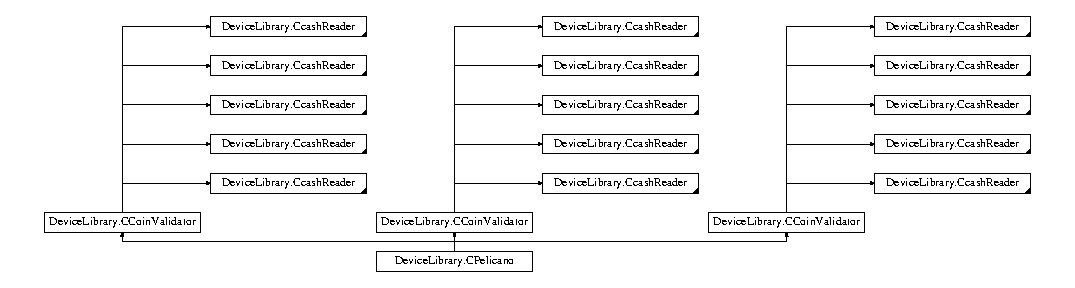
\includegraphics[height=3.420593cm]{class_device_library_1_1_c_pelicano}
\end{center}
\end{figure}
\subsection*{Public Member Functions}
\begin{DoxyCompactItemize}
\item 
bool \mbox{\hyperlink{class_device_library_1_1_c_pelicano_a8858d106bae3622a44e9ba49f5a4b98a}{Get\+Is\+Coin\+Present}} ()
\begin{DoxyCompactList}\small\item\em Vérifie si une pièce est présente dans le cointainer. \end{DoxyCompactList}\item 
override void \mbox{\hyperlink{class_device_library_1_1_c_pelicano_a38a0d7a675ff22773f5eb153fab9275a}{Task\+Check\+Event\+CV}} ()
\begin{DoxyCompactList}\small\item\em Tâche de la machine d\textquotesingle{}état du Pelicano \end{DoxyCompactList}\item 
\mbox{\hyperlink{class_device_library_1_1_c_pelicano_aef2cd2553815e501b455b7304e3b80fe}{C\+Pelicano}} ()
\begin{DoxyCompactList}\small\item\em Constructeur \end{DoxyCompactList}\end{DoxyCompactItemize}
\subsection*{Protected Types}
\begin{DoxyCompactItemize}
\item 
enum \mbox{\hyperlink{class_device_library_1_1_c_pelicano_a87743bbef8551b7349239f48892309c5}{Coin\+Present}} \{ \mbox{\hyperlink{class_device_library_1_1_c_pelicano_a87743bbef8551b7349239f48892309c5adee032dd5e2484a63525689d39d84689}{Coin\+Present.\+N\+O\+C\+O\+IN}} = 0, 
\mbox{\hyperlink{class_device_library_1_1_c_pelicano_a87743bbef8551b7349239f48892309c5a83c62b7383233ba727dc0f29fa198e22}{Coin\+Present.\+C\+O\+I\+N\+P\+R\+E\+S\+E\+NT}} = 1
 \}
\begin{DoxyCompactList}\small\item\em Enumération des présences de pièces dans le bac. \end{DoxyCompactList}\end{DoxyCompactItemize}
\subsection*{Protected Member Functions}
\begin{DoxyCompactItemize}
\item 
override void \mbox{\hyperlink{class_device_library_1_1_c_pelicano_a148ad12b2f11e1d9e6248b10a91d51df}{Check\+State}} ()
\begin{DoxyCompactList}\small\item\em Machine d\textquotesingle{}état du pelicano \end{DoxyCompactList}\end{DoxyCompactItemize}
\subsection*{Properties}
\begin{DoxyCompactItemize}
\item 
\mbox{\hyperlink{class_device_library_1_1_c_pelicano_a87743bbef8551b7349239f48892309c5}{Coin\+Present}} \mbox{\hyperlink{class_device_library_1_1_c_pelicano_ab713ffb697fd137013a1e2ade48406e2}{Coin\+In\+Container}}\hspace{0.3cm}{\ttfamily  \mbox{[}get, set\mbox{]}}
\begin{DoxyCompactList}\small\item\em Contient l\textquotesingle{}indicateur de présence de pièce dans le container. \end{DoxyCompactList}\item 
override byte \mbox{\hyperlink{class_device_library_1_1_c_pelicano_a4c21a4fe99ac28fed816dc5cb07fc794}{Opto\+States}}\hspace{0.3cm}{\ttfamily  \mbox{[}get\mbox{]}}
\begin{DoxyCompactList}\small\item\em Verification des opto-\/coupleurs \end{DoxyCompactList}\item 
override int \mbox{\hyperlink{class_device_library_1_1_c_pelicano_a74a1a52309b0331bb2f6510c698a7183}{Serial\+Number}}\hspace{0.3cm}{\ttfamily  \mbox{[}get\mbox{]}}
\begin{DoxyCompactList}\small\item\em Lecture du numéro de série du Pelicano \end{DoxyCompactList}\item 
byte \mbox{\hyperlink{class_device_library_1_1_c_pelicano_a7f5c785d7c8107df1bc22912700438bc}{Speed\+Motor}}\hspace{0.3cm}{\ttfamily  \mbox{[}get, set\mbox{]}}
\begin{DoxyCompactList}\small\item\em Renvoie la vitesse du moteur. \end{DoxyCompactList}\end{DoxyCompactItemize}
\subsection*{Additional Inherited Members}


\subsection{Detailed Description}
Class du Pelicano 



\subsection{Member Enumeration Documentation}
\mbox{\Hypertarget{class_device_library_1_1_c_pelicano_a87743bbef8551b7349239f48892309c5}\label{class_device_library_1_1_c_pelicano_a87743bbef8551b7349239f48892309c5}} 
\index{Device\+Library\+::\+C\+Pelicano@{Device\+Library\+::\+C\+Pelicano}!Coin\+Present@{Coin\+Present}}
\index{Coin\+Present@{Coin\+Present}!Device\+Library\+::\+C\+Pelicano@{Device\+Library\+::\+C\+Pelicano}}
\subsubsection{\texorpdfstring{Coin\+Present}{CoinPresent}}
{\footnotesize\ttfamily enum \mbox{\hyperlink{class_device_library_1_1_c_pelicano_a87743bbef8551b7349239f48892309c5}{Device\+Library.\+C\+Pelicano.\+Coin\+Present}}\hspace{0.3cm}{\ttfamily [strong]}, {\ttfamily [protected]}}



Enumération des présences de pièces dans le bac. 

\begin{DoxyEnumFields}{Enumerator}
\raisebox{\heightof{T}}[0pt][0pt]{\index{N\+O\+C\+O\+IN@{N\+O\+C\+O\+IN}!Device\+Library\+::\+C\+Pelicano@{Device\+Library\+::\+C\+Pelicano}}\index{Device\+Library\+::\+C\+Pelicano@{Device\+Library\+::\+C\+Pelicano}!N\+O\+C\+O\+IN@{N\+O\+C\+O\+IN}}}\mbox{\Hypertarget{class_device_library_1_1_c_pelicano_a87743bbef8551b7349239f48892309c5adee032dd5e2484a63525689d39d84689}\label{class_device_library_1_1_c_pelicano_a87743bbef8551b7349239f48892309c5adee032dd5e2484a63525689d39d84689}} 
N\+O\+C\+O\+IN&Pas de pièce dans le container. \\
\hline

\raisebox{\heightof{T}}[0pt][0pt]{\index{C\+O\+I\+N\+P\+R\+E\+S\+E\+NT@{C\+O\+I\+N\+P\+R\+E\+S\+E\+NT}!Device\+Library\+::\+C\+Pelicano@{Device\+Library\+::\+C\+Pelicano}}\index{Device\+Library\+::\+C\+Pelicano@{Device\+Library\+::\+C\+Pelicano}!C\+O\+I\+N\+P\+R\+E\+S\+E\+NT@{C\+O\+I\+N\+P\+R\+E\+S\+E\+NT}}}\mbox{\Hypertarget{class_device_library_1_1_c_pelicano_a87743bbef8551b7349239f48892309c5a83c62b7383233ba727dc0f29fa198e22}\label{class_device_library_1_1_c_pelicano_a87743bbef8551b7349239f48892309c5a83c62b7383233ba727dc0f29fa198e22}} 
C\+O\+I\+N\+P\+R\+E\+S\+E\+NT&Au monis une pièce présent dans le container. \\
\hline

\end{DoxyEnumFields}


\subsection{Constructor \& Destructor Documentation}
\mbox{\Hypertarget{class_device_library_1_1_c_pelicano_aef2cd2553815e501b455b7304e3b80fe}\label{class_device_library_1_1_c_pelicano_aef2cd2553815e501b455b7304e3b80fe}} 
\index{Device\+Library\+::\+C\+Pelicano@{Device\+Library\+::\+C\+Pelicano}!C\+Pelicano@{C\+Pelicano}}
\index{C\+Pelicano@{C\+Pelicano}!Device\+Library\+::\+C\+Pelicano@{Device\+Library\+::\+C\+Pelicano}}
\subsubsection{\texorpdfstring{C\+Pelicano()}{CPelicano()}}
{\footnotesize\ttfamily Device\+Library.\+C\+Pelicano.\+C\+Pelicano (\begin{DoxyParamCaption}{ }\end{DoxyParamCaption})\hspace{0.3cm}{\ttfamily [inline]}}



Constructeur 



\subsection{Member Function Documentation}
\mbox{\Hypertarget{class_device_library_1_1_c_pelicano_a148ad12b2f11e1d9e6248b10a91d51df}\label{class_device_library_1_1_c_pelicano_a148ad12b2f11e1d9e6248b10a91d51df}} 
\index{Device\+Library\+::\+C\+Pelicano@{Device\+Library\+::\+C\+Pelicano}!Check\+State@{Check\+State}}
\index{Check\+State@{Check\+State}!Device\+Library\+::\+C\+Pelicano@{Device\+Library\+::\+C\+Pelicano}}
\subsubsection{\texorpdfstring{Check\+State()}{CheckState()}}
{\footnotesize\ttfamily override void Device\+Library.\+C\+Pelicano.\+Check\+State (\begin{DoxyParamCaption}{ }\end{DoxyParamCaption})\hspace{0.3cm}{\ttfamily [inline]}, {\ttfamily [protected]}, {\ttfamily [virtual]}}



Machine d\textquotesingle{}état du pelicano 



Reimplemented from \mbox{\hyperlink{class_device_library_1_1_c_coin_validator_ad5060d28baf7c2abedc788c6bcdcb02d}{Device\+Library.\+C\+Coin\+Validator}}.

\mbox{\Hypertarget{class_device_library_1_1_c_pelicano_a8858d106bae3622a44e9ba49f5a4b98a}\label{class_device_library_1_1_c_pelicano_a8858d106bae3622a44e9ba49f5a4b98a}} 
\index{Device\+Library\+::\+C\+Pelicano@{Device\+Library\+::\+C\+Pelicano}!Get\+Is\+Coin\+Present@{Get\+Is\+Coin\+Present}}
\index{Get\+Is\+Coin\+Present@{Get\+Is\+Coin\+Present}!Device\+Library\+::\+C\+Pelicano@{Device\+Library\+::\+C\+Pelicano}}
\subsubsection{\texorpdfstring{Get\+Is\+Coin\+Present()}{GetIsCoinPresent()}}
{\footnotesize\ttfamily bool Device\+Library.\+C\+Pelicano.\+Get\+Is\+Coin\+Present (\begin{DoxyParamCaption}{ }\end{DoxyParamCaption})\hspace{0.3cm}{\ttfamily [inline]}}



Vérifie si une pièce est présente dans le cointainer. 

\begin{DoxyReturn}{Returns}
true si au moins une pièce est présente dans le bol~\newline
false s\textquotesingle{}il n\textquotesingle{}y a pas de pièce 
\end{DoxyReturn}
\mbox{\Hypertarget{class_device_library_1_1_c_pelicano_a38a0d7a675ff22773f5eb153fab9275a}\label{class_device_library_1_1_c_pelicano_a38a0d7a675ff22773f5eb153fab9275a}} 
\index{Device\+Library\+::\+C\+Pelicano@{Device\+Library\+::\+C\+Pelicano}!Task\+Check\+Event\+CV@{Task\+Check\+Event\+CV}}
\index{Task\+Check\+Event\+CV@{Task\+Check\+Event\+CV}!Device\+Library\+::\+C\+Pelicano@{Device\+Library\+::\+C\+Pelicano}}
\subsubsection{\texorpdfstring{Task\+Check\+Event\+C\+V()}{TaskCheckEventCV()}}
{\footnotesize\ttfamily override void Device\+Library.\+C\+Pelicano.\+Task\+Check\+Event\+CV (\begin{DoxyParamCaption}{ }\end{DoxyParamCaption})\hspace{0.3cm}{\ttfamily [inline]}, {\ttfamily [virtual]}}



Tâche de la machine d\textquotesingle{}état du Pelicano 



Reimplemented from \mbox{\hyperlink{class_device_library_1_1_c_coin_validator_a0e406f9e175eb8d295fe7406e6a948af}{Device\+Library.\+C\+Coin\+Validator}}.



\subsection{Property Documentation}
\mbox{\Hypertarget{class_device_library_1_1_c_pelicano_ab713ffb697fd137013a1e2ade48406e2}\label{class_device_library_1_1_c_pelicano_ab713ffb697fd137013a1e2ade48406e2}} 
\index{Device\+Library\+::\+C\+Pelicano@{Device\+Library\+::\+C\+Pelicano}!Coin\+In\+Container@{Coin\+In\+Container}}
\index{Coin\+In\+Container@{Coin\+In\+Container}!Device\+Library\+::\+C\+Pelicano@{Device\+Library\+::\+C\+Pelicano}}
\subsubsection{\texorpdfstring{Coin\+In\+Container}{CoinInContainer}}
{\footnotesize\ttfamily \mbox{\hyperlink{class_device_library_1_1_c_pelicano_a87743bbef8551b7349239f48892309c5}{Coin\+Present}} Device\+Library.\+C\+Pelicano.\+Coin\+In\+Container\hspace{0.3cm}{\ttfamily [get]}, {\ttfamily [set]}, {\ttfamily [protected]}}



Contient l\textquotesingle{}indicateur de présence de pièce dans le container. 

\mbox{\Hypertarget{class_device_library_1_1_c_pelicano_a4c21a4fe99ac28fed816dc5cb07fc794}\label{class_device_library_1_1_c_pelicano_a4c21a4fe99ac28fed816dc5cb07fc794}} 
\index{Device\+Library\+::\+C\+Pelicano@{Device\+Library\+::\+C\+Pelicano}!Opto\+States@{Opto\+States}}
\index{Opto\+States@{Opto\+States}!Device\+Library\+::\+C\+Pelicano@{Device\+Library\+::\+C\+Pelicano}}
\subsubsection{\texorpdfstring{Opto\+States}{OptoStates}}
{\footnotesize\ttfamily override byte Device\+Library.\+C\+Pelicano.\+Opto\+States\hspace{0.3cm}{\ttfamily [get]}}



Verification des opto-\/coupleurs 

Header 236\mbox{\Hypertarget{class_device_library_1_1_c_pelicano_a74a1a52309b0331bb2f6510c698a7183}\label{class_device_library_1_1_c_pelicano_a74a1a52309b0331bb2f6510c698a7183}} 
\index{Device\+Library\+::\+C\+Pelicano@{Device\+Library\+::\+C\+Pelicano}!Serial\+Number@{Serial\+Number}}
\index{Serial\+Number@{Serial\+Number}!Device\+Library\+::\+C\+Pelicano@{Device\+Library\+::\+C\+Pelicano}}
\subsubsection{\texorpdfstring{Serial\+Number}{SerialNumber}}
{\footnotesize\ttfamily override int Device\+Library.\+C\+Pelicano.\+Serial\+Number\hspace{0.3cm}{\ttfamily [get]}}



Lecture du numéro de série du Pelicano 

\begin{DoxyReturn}{Returns}
Le numéro de série
\end{DoxyReturn}
\mbox{\Hypertarget{class_device_library_1_1_c_pelicano_a7f5c785d7c8107df1bc22912700438bc}\label{class_device_library_1_1_c_pelicano_a7f5c785d7c8107df1bc22912700438bc}} 
\index{Device\+Library\+::\+C\+Pelicano@{Device\+Library\+::\+C\+Pelicano}!Speed\+Motor@{Speed\+Motor}}
\index{Speed\+Motor@{Speed\+Motor}!Device\+Library\+::\+C\+Pelicano@{Device\+Library\+::\+C\+Pelicano}}
\subsubsection{\texorpdfstring{Speed\+Motor}{SpeedMotor}}
{\footnotesize\ttfamily byte Device\+Library.\+C\+Pelicano.\+Speed\+Motor\hspace{0.3cm}{\ttfamily [get]}, {\ttfamily [set]}}



Renvoie la vitesse du moteur. 

\begin{DoxyReturn}{Returns}
La vitesse du moteur en pourcentage.~\newline
0 si la command ne renvoit rien. 
\end{DoxyReturn}


The documentation for this class was generated from the following files\+:\begin{DoxyCompactItemize}
\item 
D\+:/\+Projets/\+A\+T\+M\+B/\+S\+O\+F\+T/\+Atmb\+Devices/\+Device\+Library/C\+Pelicano.\+Cmd\+Motors.\+cs\item 
D\+:/\+Projets/\+A\+T\+M\+B/\+S\+O\+F\+T/\+Atmb\+Devices/\+Device\+Library/C\+Pelicano.\+cs\end{DoxyCompactItemize}

\hypertarget{class_device_library_1_1_c_canal_1_1_c_sorter}{}\section{Device\+Library.\+C\+Canal.\+C\+Sorter Class Reference}
\label{class_device_library_1_1_c_canal_1_1_c_sorter}\index{Device\+Library.\+C\+Canal.\+C\+Sorter@{Device\+Library.\+C\+Canal.\+C\+Sorter}}


Class gérant les informations concernant un chemin de triage d\textquotesingle{}un canal  


\subsection*{Public Member Functions}
\begin{DoxyCompactItemize}
\item 
void \mbox{\hyperlink{class_device_library_1_1_c_canal_1_1_c_sorter_a3e3bd854bcc07374dbf12baefe6afea4}{Set\+Sorter\+Path}} (byte path\+Sorter)
\begin{DoxyCompactList}\small\item\em Definie le chemin utilisé par le trieur pour ce canal. \end{DoxyCompactList}\item 
\mbox{\hyperlink{class_device_library_1_1_c_canal_1_1_c_sorter_a45e0fa5899f6d78de268976c1a9f1887}{C\+Sorter}} (\mbox{\hyperlink{class_device_library_1_1_c_canal}{C\+Canal}} owner)
\begin{DoxyCompactList}\small\item\em Constructeur \end{DoxyCompactList}\end{DoxyCompactItemize}
\subsection*{Public Attributes}
\begin{DoxyCompactItemize}
\item 
byte \mbox{[}$\,$\mbox{]} \mbox{\hyperlink{class_device_library_1_1_c_canal_1_1_c_sorter_af92b28db721034603d820227b5b544fe}{Over\+Path}}
\begin{DoxyCompactList}\small\item\em Chemin de substitusion. \end{DoxyCompactList}\end{DoxyCompactItemize}
\subsection*{Properties}
\begin{DoxyCompactItemize}
\item 
byte \mbox{\hyperlink{class_device_library_1_1_c_canal_1_1_c_sorter_a9fefa95f8e5231ef8361faffe80c50a1}{Path\+Sorter}}\hspace{0.3cm}{\ttfamily  \mbox{[}get, set\mbox{]}}
\begin{DoxyCompactList}\small\item\em Chemin utilisé dans le trieur (de 1 à 8) \end{DoxyCompactList}\end{DoxyCompactItemize}


\subsection{Detailed Description}
Class gérant les informations concernant un chemin de triage d\textquotesingle{}un canal 



\subsection{Constructor \& Destructor Documentation}
\mbox{\Hypertarget{class_device_library_1_1_c_canal_1_1_c_sorter_a45e0fa5899f6d78de268976c1a9f1887}\label{class_device_library_1_1_c_canal_1_1_c_sorter_a45e0fa5899f6d78de268976c1a9f1887}} 
\index{Device\+Library\+::\+C\+Canal\+::\+C\+Sorter@{Device\+Library\+::\+C\+Canal\+::\+C\+Sorter}!C\+Sorter@{C\+Sorter}}
\index{C\+Sorter@{C\+Sorter}!Device\+Library\+::\+C\+Canal\+::\+C\+Sorter@{Device\+Library\+::\+C\+Canal\+::\+C\+Sorter}}
\subsubsection{\texorpdfstring{C\+Sorter()}{CSorter()}}
{\footnotesize\ttfamily Device\+Library.\+C\+Canal.\+C\+Sorter.\+C\+Sorter (\begin{DoxyParamCaption}\item[{\mbox{\hyperlink{class_device_library_1_1_c_canal}{C\+Canal}}}]{owner }\end{DoxyParamCaption})\hspace{0.3cm}{\ttfamily [inline]}}



Constructeur 


\begin{DoxyParams}{Parameters}
{\em owner} & Canal correspondant\\
\hline
\end{DoxyParams}


\subsection{Member Function Documentation}
\mbox{\Hypertarget{class_device_library_1_1_c_canal_1_1_c_sorter_a3e3bd854bcc07374dbf12baefe6afea4}\label{class_device_library_1_1_c_canal_1_1_c_sorter_a3e3bd854bcc07374dbf12baefe6afea4}} 
\index{Device\+Library\+::\+C\+Canal\+::\+C\+Sorter@{Device\+Library\+::\+C\+Canal\+::\+C\+Sorter}!Set\+Sorter\+Path@{Set\+Sorter\+Path}}
\index{Set\+Sorter\+Path@{Set\+Sorter\+Path}!Device\+Library\+::\+C\+Canal\+::\+C\+Sorter@{Device\+Library\+::\+C\+Canal\+::\+C\+Sorter}}
\subsubsection{\texorpdfstring{Set\+Sorter\+Path()}{SetSorterPath()}}
{\footnotesize\ttfamily void Device\+Library.\+C\+Canal.\+C\+Sorter.\+Set\+Sorter\+Path (\begin{DoxyParamCaption}\item[{byte}]{path\+Sorter }\end{DoxyParamCaption})\hspace{0.3cm}{\ttfamily [inline]}}



Definie le chemin utilisé par le trieur pour ce canal. 


\begin{DoxyParams}{Parameters}
{\em path\+Sorter} & Chemin dans le trieur\\
\hline
\end{DoxyParams}


\subsection{Member Data Documentation}
\mbox{\Hypertarget{class_device_library_1_1_c_canal_1_1_c_sorter_af92b28db721034603d820227b5b544fe}\label{class_device_library_1_1_c_canal_1_1_c_sorter_af92b28db721034603d820227b5b544fe}} 
\index{Device\+Library\+::\+C\+Canal\+::\+C\+Sorter@{Device\+Library\+::\+C\+Canal\+::\+C\+Sorter}!Over\+Path@{Over\+Path}}
\index{Over\+Path@{Over\+Path}!Device\+Library\+::\+C\+Canal\+::\+C\+Sorter@{Device\+Library\+::\+C\+Canal\+::\+C\+Sorter}}
\subsubsection{\texorpdfstring{Over\+Path}{OverPath}}
{\footnotesize\ttfamily byte \mbox{[}$\,$\mbox{]} Device\+Library.\+C\+Canal.\+C\+Sorter.\+Over\+Path}



Chemin de substitusion. 



\subsection{Property Documentation}
\mbox{\Hypertarget{class_device_library_1_1_c_canal_1_1_c_sorter_a9fefa95f8e5231ef8361faffe80c50a1}\label{class_device_library_1_1_c_canal_1_1_c_sorter_a9fefa95f8e5231ef8361faffe80c50a1}} 
\index{Device\+Library\+::\+C\+Canal\+::\+C\+Sorter@{Device\+Library\+::\+C\+Canal\+::\+C\+Sorter}!Path\+Sorter@{Path\+Sorter}}
\index{Path\+Sorter@{Path\+Sorter}!Device\+Library\+::\+C\+Canal\+::\+C\+Sorter@{Device\+Library\+::\+C\+Canal\+::\+C\+Sorter}}
\subsubsection{\texorpdfstring{Path\+Sorter}{PathSorter}}
{\footnotesize\ttfamily byte Device\+Library.\+C\+Canal.\+C\+Sorter.\+Path\+Sorter\hspace{0.3cm}{\ttfamily [get]}, {\ttfamily [set]}}



Chemin utilisé dans le trieur (de 1 à 8) 



The documentation for this class was generated from the following file\+:\begin{DoxyCompactItemize}
\item 
D\+:/\+Projets/\+A\+T\+M\+B/\+S\+O\+F\+T/\+Atmb\+Devices/\+Device\+Library/C\+Sorter.\+cs\end{DoxyCompactItemize}

\hypertarget{class_device_library_1_1messages_text}{}\section{Device\+Library.\+messages\+Text Class Reference}
\label{class_device_library_1_1messages_text}\index{Device\+Library.\+messages\+Text@{Device\+Library.\+messages\+Text}}


Une classe de ressource fortement typée destinée, entre autres, à la consultation des chaînes localisées.  


\subsection*{Properties}
\begin{DoxyCompactItemize}
\item 
static global\+::\+System.\+Resources.\+Resource\+Manager \mbox{\hyperlink{class_device_library_1_1messages_text_a031636cf4621ff551aa62648e5c08b4b}{Resource\+Manager}}\hspace{0.3cm}{\ttfamily  \mbox{[}get\mbox{]}}
\begin{DoxyCompactList}\small\item\em Retourne l\textquotesingle{}instance Resource\+Manager mise en cache utilisée par cette classe. \end{DoxyCompactList}\item 
static global\+::\+System.\+Globalization.\+Culture\+Info \mbox{\hyperlink{class_device_library_1_1messages_text_abcb12fd4a215b678e9b5abda167ce8f6}{Culture}}\hspace{0.3cm}{\ttfamily  \mbox{[}get, set\mbox{]}}
\begin{DoxyCompactList}\small\item\em Remplace la propriété Current\+U\+I\+Culture du thread actuel pour toutes les recherches de ressources à l\textquotesingle{}aide de cette classe de ressource fortement typée. \end{DoxyCompactList}\item 
static string \mbox{\hyperlink{class_device_library_1_1messages_text_a1b8c8f4de98cd13953372dac6cf288da}{activation\+CV}}\hspace{0.3cm}{\ttfamily  \mbox{[}get\mbox{]}}
\begin{DoxyCompactList}\small\item\em Recherche une chaîne localisée semblable à Activation du \{0\}. \end{DoxyCompactList}\item 
static string \mbox{\hyperlink{class_device_library_1_1messages_text_a755549427f23616566b9993e8ea52a22}{build\+Code}}\hspace{0.3cm}{\ttfamily  \mbox{[}get\mbox{]}}
\begin{DoxyCompactList}\small\item\em Recherche une chaîne localisée semblable à Le build code du \{0\} est "\{1\}". \end{DoxyCompactList}\item 
static string \mbox{\hyperlink{class_device_library_1_1messages_text_aae08998942f40ad4e17d68f70572f27b}{bus\+O\+Kfinded}}\hspace{0.3cm}{\ttfamily  \mbox{[}get\mbox{]}}
\begin{DoxyCompactList}\small\item\em Recherche une chaîne localisée semblable à Bus cc\+Talk trouvé sur le port C\+OM\{0\}.. \end{DoxyCompactList}\item 
static string \mbox{\hyperlink{class_device_library_1_1messages_text_a5aba326853a8c8f79f70053306ee819c}{call\+Dll}}\hspace{0.3cm}{\ttfamily  \mbox{[}get\mbox{]}}
\begin{DoxyCompactList}\small\item\em Recherche une chaîne localisée semblable à Appel de la dll. \end{DoxyCompactList}\item 
static string \mbox{\hyperlink{class_device_library_1_1messages_text_adc962171c994c63312d316f13b046d2c}{cc\+Talk\+Instance}}\hspace{0.3cm}{\ttfamily  \mbox{[}get\mbox{]}}
\begin{DoxyCompactList}\small\item\em Recherche une chaîne localisée semblable à Instanciation cc\+Talk.. \end{DoxyCompactList}\item 
static string \mbox{\hyperlink{class_device_library_1_1messages_text_ac961f592dd67ea083a505482617c823b}{cmd\+Motor\+Pelicano}}\hspace{0.3cm}{\ttfamily  \mbox{[}get\mbox{]}}
\begin{DoxyCompactList}\small\item\em Recherche une chaîne localisée semblable à Commande \{0\} moteur du pelicano . \end{DoxyCompactList}\item 
static string \mbox{\hyperlink{class_device_library_1_1messages_text_aa5a99445dd360fad1b310b74d9be7bf6}{cmd\+Motor\+Pelicano\+In\+Progress}}\hspace{0.3cm}{\ttfamily  \mbox{[}get\mbox{]}}
\begin{DoxyCompactList}\small\item\em Recherche une chaîne localisée semblable à Le moteur du pelicano est activé.. \end{DoxyCompactList}\item 
static string \mbox{\hyperlink{class_device_library_1_1messages_text_a5ae581131aa224503a54e4a29aa82916}{cmd\+Motor\+Pelicano\+Mode}}\hspace{0.3cm}{\ttfamily  \mbox{[}get\mbox{]}}
\begin{DoxyCompactList}\small\item\em Recherche une chaîne localisée semblable à Activation du moteur du pelicano commande \{0\}. \end{DoxyCompactList}\item 
static string \mbox{\hyperlink{class_device_library_1_1messages_text_a11e70bc1bf9a2de56400fbab90cb153f}{cmd\+Self\+Test}}\hspace{0.3cm}{\ttfamily  \mbox{[}get\mbox{]}}
\begin{DoxyCompactList}\small\item\em Recherche une chaîne localisée semblable à Effectue un self test du \{0\}. \end{DoxyCompactList}\item 
static string \mbox{\hyperlink{class_device_library_1_1messages_text_ada1347a59a5832cbebb4ed1fe62a76d4}{data\+Base\+Version}}\hspace{0.3cm}{\ttfamily  \mbox{[}get\mbox{]}}
\begin{DoxyCompactList}\small\item\em Recherche une chaîne localisée semblable à La version de la data base du \{0\} est "\{1\}". \end{DoxyCompactList}\item 
static string \mbox{\hyperlink{class_device_library_1_1messages_text_ab25fcc8955786b9eb2cc6a0eeb512a0e}{deactivation\+CV}}\hspace{0.3cm}{\ttfamily  \mbox{[}get\mbox{]}}
\begin{DoxyCompactList}\small\item\em Recherche une chaîne localisée semblable à Desactivation du \{0\}. \end{DoxyCompactList}\item 
static string \mbox{\hyperlink{class_device_library_1_1messages_text_ab9931d675639d2f20b12a5b9d7247d76}{delay\+Polling}}\hspace{0.3cm}{\ttfamily  \mbox{[}get\mbox{]}}
\begin{DoxyCompactList}\small\item\em Recherche une chaîne localisée semblable à Delai maximum entre 2 commande pour le \{0\} est de \{1\} ms. \end{DoxyCompactList}\item 
static string \mbox{\hyperlink{class_device_library_1_1messages_text_a616c0d5ff9f3a4f77f95b8402e3d17b5}{echo}}\hspace{0.3cm}{\ttfamily  \mbox{[}get\mbox{]}}
\begin{DoxyCompactList}\small\item\em Recherche une chaîne localisée semblable à Echo \+: . \end{DoxyCompactList}\item 
static string \mbox{\hyperlink{class_device_library_1_1messages_text_a2f05f0441e8bb2a403b65e2ed0839e2d}{equipement\+ID}}\hspace{0.3cm}{\ttfamily  \mbox{[}get\mbox{]}}
\begin{DoxyCompactList}\small\item\em Recherche une chaîne localisée semblable à L\textquotesingle{}identitification de l\textquotesingle{}equipement est "\{0\}". \end{DoxyCompactList}\item 
static string \mbox{\hyperlink{class_device_library_1_1messages_text_a692ddbde572309d1f80363365fd514e9}{erreur}}\hspace{0.3cm}{\ttfamily  \mbox{[}get\mbox{]}}
\begin{DoxyCompactList}\small\item\em Recherche une chaîne localisée semblable à E\+R\+R\+E\+UR \{0\} \{1\} \{2\}.. \end{DoxyCompactList}\item 
static string \mbox{\hyperlink{class_device_library_1_1messages_text_a9b8554d38ab9c2799d5405e2f894cf82}{erreur\+Cmd}}\hspace{0.3cm}{\ttfamily  \mbox{[}get\mbox{]}}
\begin{DoxyCompactList}\small\item\em Recherche une chaîne localisée semblable à Impossible d\textquotesingle{}effectuer la commande \{0\} sur le \{1\}. \end{DoxyCompactList}\item 
static string \mbox{\hyperlink{class_device_library_1_1messages_text_a9bd55afe4b9caa13b0d861fc4c3ff24f}{erreur\+Polling\+Priority}}\hspace{0.3cm}{\ttfamily  \mbox{[}get\mbox{]}}
\begin{DoxyCompactList}\small\item\em Recherche une chaîne localisée semblable à Impossible de lire la délai du polling \{0\}. \end{DoxyCompactList}\item 
static string \mbox{\hyperlink{class_device_library_1_1messages_text_a54b35fb372930fed5dc13a77e060396c}{erreur\+Port}}\hspace{0.3cm}{\ttfamily  \mbox{[}get\mbox{]}}
\begin{DoxyCompactList}\small\item\em Recherche une chaîne localisée semblable à Erreur de conversion du numero de port \{0\}.. \end{DoxyCompactList}\item 
static string \mbox{\hyperlink{class_device_library_1_1messages_text_aa59ba4427bc96cde7bd3f125a279f09c}{err\+Get\+Inhibit\+Status}}\hspace{0.3cm}{\ttfamily  \mbox{[}get\mbox{]}}
\begin{DoxyCompactList}\small\item\em Recherche une chaîne localisée semblable à Impossible de lire le masque d\textquotesingle{}inhibition des canaux du \{0\}. \end{DoxyCompactList}\item 
static string \mbox{\hyperlink{class_device_library_1_1messages_text_a56487b103b700f2efc304a3ab0a75d1a}{err\+Inhibit\+Status}}\hspace{0.3cm}{\ttfamily  \mbox{[}get\mbox{]}}
\begin{DoxyCompactList}\small\item\em Recherche une chaîne localisée semblable à Impossible de modifier l\textquotesingle{}habitation des canaux du \{0\}. \end{DoxyCompactList}\item 
static string \mbox{\hyperlink{class_device_library_1_1messages_text_ad9c4ce7df2d9a97fb037a6b2fe1a01fe}{err\+Master\+Inhibit\+Status}}\hspace{0.3cm}{\ttfamily  \mbox{[}get\mbox{]}}
\begin{DoxyCompactList}\small\item\em Recherche une chaîne localisée semblable à Impossible d\textquotesingle{}enregistrer le master inhibit status du \{0\}. \end{DoxyCompactList}\item 
static string \mbox{\hyperlink{class_device_library_1_1messages_text_a457477e9ee134856647bf051d74293ea}{err\+Motor\+Pelicano}}\hspace{0.3cm}{\ttfamily  \mbox{[}get\mbox{]}}
\begin{DoxyCompactList}\small\item\em Recherche une chaîne localisée semblable à Impossible d\textquotesingle{}executer la commande sur le moteur du pelicano. \end{DoxyCompactList}\item 
static string \mbox{\hyperlink{class_device_library_1_1messages_text_a2ff352411ad8af876fe7fb650e091aa5}{get\+Build\+Code}}\hspace{0.3cm}{\ttfamily  \mbox{[}get\mbox{]}}
\begin{DoxyCompactList}\small\item\em Recherche une chaîne localisée semblable à Demande du code de fabrication du \{0\}. \end{DoxyCompactList}\item 
static string \mbox{\hyperlink{class_device_library_1_1messages_text_a76120e98024c293607801a782c164899}{get\+Byte}}\hspace{0.3cm}{\ttfamily  \mbox{[}get\mbox{]}}
\begin{DoxyCompactList}\small\item\em Recherche une chaîne localisée semblable à Lecture de l\textquotesingle{}octet dans le \{0\}. \end{DoxyCompactList}\item 
static string \mbox{\hyperlink{class_device_library_1_1messages_text_ab9e7a38bdab6ee7cce1c2f701e1e5fa1}{get\+Data\+Base\+Version}}\hspace{0.3cm}{\ttfamily  \mbox{[}get\mbox{]}}
\begin{DoxyCompactList}\small\item\em Recherche une chaîne localisée semblable à Demande de la version de la data base du \{0\}. \end{DoxyCompactList}\item 
static string \mbox{\hyperlink{class_device_library_1_1messages_text_afd4b16d2d28ef8fc8e9152e92ee3875f}{get\+Equipement\+ID}}\hspace{0.3cm}{\ttfamily  \mbox{[}get\mbox{]}}
\begin{DoxyCompactList}\small\item\em Recherche une chaîne localisée semblable à Le périphérique est un \{0\}. \end{DoxyCompactList}\item 
static string \mbox{\hyperlink{class_device_library_1_1messages_text_ae354123829e86b8cf6e13deaa2cda560}{get\+Inhibit\+Status}}\hspace{0.3cm}{\ttfamily  \mbox{[}get\mbox{]}}
\begin{DoxyCompactList}\small\item\em Recherche une chaîne localisée semblable à Lecture du masque d\textquotesingle{}inhibitiion des canaux du \{0\}. \end{DoxyCompactList}\item 
static string \mbox{\hyperlink{class_device_library_1_1messages_text_a98d96d1497375fafe0595cd8b05cfd35}{get\+Manufacturer}}\hspace{0.3cm}{\ttfamily  \mbox{[}get\mbox{]}}
\begin{DoxyCompactList}\small\item\em Recherche une chaîne localisée semblable à Demande de l\textquotesingle{}identifiant du fabricant du \{0\}. \end{DoxyCompactList}\item 
static string \mbox{\hyperlink{class_device_library_1_1messages_text_ab90f77c2226516821994a2f6c1618ba9}{get\+Master\+Inhibt}}\hspace{0.3cm}{\ttfamily  \mbox{[}get\mbox{]}}
\begin{DoxyCompactList}\small\item\em Recherche une chaîne localisée semblable à Lecture de l\textquotesingle{}inhibition du \{0\}. \end{DoxyCompactList}\item 
static string \mbox{\hyperlink{class_device_library_1_1messages_text_ad09a1b8efb45bbb4d1f9724decdb84d9}{get\+Polling}}\hspace{0.3cm}{\ttfamily  \mbox{[}get\mbox{]}}
\begin{DoxyCompactList}\small\item\em Recherche une chaîne localisée semblable à Demande du délai de polling pour le \{0\}. \end{DoxyCompactList}\item 
static string \mbox{\hyperlink{class_device_library_1_1messages_text_a38c36d19079298c6c9dbd63befe471bc}{get\+Product\+Code}}\hspace{0.3cm}{\ttfamily  \mbox{[}get\mbox{]}}
\begin{DoxyCompactList}\small\item\em Recherche une chaîne localisée semblable à Demande du code produit du \{0\}. \end{DoxyCompactList}\item 
static string \mbox{\hyperlink{class_device_library_1_1messages_text_adf25abdc6ae9b774a1acf5ca9c3e774c}{get\+SN}}\hspace{0.3cm}{\ttfamily  \mbox{[}get\mbox{]}}
\begin{DoxyCompactList}\small\item\em Recherche une chaîne localisée semblable à Demande du numéro de série du \{0\}. \end{DoxyCompactList}\item 
static string \mbox{\hyperlink{class_device_library_1_1messages_text_a57d987d8f74d2176c72e5f6e29b42fc2}{get\+S\+W\+Rev}}\hspace{0.3cm}{\ttfamily  \mbox{[}get\mbox{]}}
\begin{DoxyCompactList}\small\item\em Recherche une chaîne localisée semblable à Demande de la vérivision software du \{0\}. \end{DoxyCompactList}\item 
static string \mbox{\hyperlink{class_device_library_1_1messages_text_a41967611d2c8b9d237599dd156a13dd8}{get\+Text}}\hspace{0.3cm}{\ttfamily  \mbox{[}get\mbox{]}}
\begin{DoxyCompactList}\small\item\em Recherche une chaîne localisée semblable à Lecture de la chaine A\+S\+C\+II dans le \{0\}. \end{DoxyCompactList}\item 
static string \mbox{\hyperlink{class_device_library_1_1messages_text_a4e9189c04771bbd6e96ba7f9d5d515fc}{hello}}\hspace{0.3cm}{\ttfamily  \mbox{[}get\mbox{]}}
\begin{DoxyCompactList}\small\item\em Recherche une chaîne localisée semblable à H\+E\+L\+LO. \end{DoxyCompactList}\item 
static string \mbox{\hyperlink{class_device_library_1_1messages_text_a4beee20720447145e0de98bb1cf44e66}{inhibit\+Status}}\hspace{0.3cm}{\ttfamily  \mbox{[}get\mbox{]}}
\begin{DoxyCompactList}\small\item\em Recherche une chaîne localisée semblable à Modifie l\textquotesingle{}habilitation des canaux du \{0\} \{1\} \{2\}. \end{DoxyCompactList}\item 
static string \mbox{\hyperlink{class_device_library_1_1messages_text_ac37e35f9f795175e6dca7d0b49b33637}{inhibit\+Status\+Result}}\hspace{0.3cm}{\ttfamily  \mbox{[}get\mbox{]}}
\begin{DoxyCompactList}\small\item\em Recherche une chaîne localisée semblable à le \{0\} est \{1\}. \end{DoxyCompactList}\item 
static string \mbox{\hyperlink{class_device_library_1_1messages_text_a2f62050bea514c3f25710deb511535dc}{manufacturer}}\hspace{0.3cm}{\ttfamily  \mbox{[}get\mbox{]}}
\begin{DoxyCompactList}\small\item\em Recherche une chaîne localisée semblable à L\textquotesingle{}identifiant du fabricant du \{0\} est "\{1\}". \end{DoxyCompactList}\item 
static string \mbox{\hyperlink{class_device_library_1_1messages_text_af19cd4177e26f024d4d1a709f51c63b9}{nocc\+Talk\+Device}}\hspace{0.3cm}{\ttfamily  \mbox{[}get\mbox{]}}
\begin{DoxyCompactList}\small\item\em Recherche une chaîne localisée semblable à \{0\} Lecture impossible, pas de bus cc\+Talk ou pas de periphérique cc\+Talk reconnu ou periphérique HS sur le port \{1\}.. \end{DoxyCompactList}\item 
static string \mbox{\hyperlink{class_device_library_1_1messages_text_ac150c27572b319dde35b8ac2b76e5801}{polling}}\hspace{0.3cm}{\ttfamily  \mbox{[}get\mbox{]}}
\begin{DoxyCompactList}\small\item\em Recherche une chaîne localisée semblable à Lecture du délai de polling. \end{DoxyCompactList}\item 
static string \mbox{\hyperlink{class_device_library_1_1messages_text_af981c9675348c68009065abaf1a00b28}{product\+Code}}\hspace{0.3cm}{\ttfamily  \mbox{[}get\mbox{]}}
\begin{DoxyCompactList}\small\item\em Recherche une chaîne localisée semblable à Le code produit du \{0\} est "\{1\}". \end{DoxyCompactList}\item 
static string \mbox{\hyperlink{class_device_library_1_1messages_text_a639a4669a24e5f9579bdd3815268d806}{read\+Answer\+Device}}\hspace{0.3cm}{\ttfamily  \mbox{[}get\mbox{]}}
\begin{DoxyCompactList}\small\item\em Recherche une chaîne localisée semblable à Lecture de la réponse du périphérique.. \end{DoxyCompactList}\item 
static string \mbox{\hyperlink{class_device_library_1_1messages_text_aac828c24757eef357df7ede8980d5f5d}{read\+Echo}}\hspace{0.3cm}{\ttfamily  \mbox{[}get\mbox{]}}
\begin{DoxyCompactList}\small\item\em Recherche une chaîne localisée semblable à Lecture de l\textquotesingle{}écho.. \end{DoxyCompactList}\item 
static string \mbox{\hyperlink{class_device_library_1_1messages_text_a3bce2e18d1b8dbc3d29446f4c1fc7cc7}{search\+\_\+cc\+Talk}}\hspace{0.3cm}{\ttfamily  \mbox{[}get\mbox{]}}
\begin{DoxyCompactList}\small\item\em Recherche une chaîne localisée semblable à Recherche du port série cc\+Talk.. \end{DoxyCompactList}\item 
static string \mbox{\hyperlink{class_device_library_1_1messages_text_a848d1437acc274997c7e914263ed490a}{self\+Test}}\hspace{0.3cm}{\ttfamily  \mbox{[}get\mbox{]}}
\begin{DoxyCompactList}\small\item\em Recherche une chaîne localisée semblable à Le résultat du self test du \{0\} est \{1\}. \end{DoxyCompactList}\item 
static string \mbox{\hyperlink{class_device_library_1_1messages_text_a6cdf49693beb3766d1b9a2ca4c582a43}{send\+Cmd}}\hspace{0.3cm}{\ttfamily  \mbox{[}get\mbox{]}}
\begin{DoxyCompactList}\small\item\em Recherche une chaîne localisée semblable à Envoi de la commande "\{0\}" au \{1\}.. \end{DoxyCompactList}\item 
static string \mbox{\hyperlink{class_device_library_1_1messages_text_a36eee29e70368828dc0fb2ff7ec98ac0}{send\+Master\+Inhibit\+Status}}\hspace{0.3cm}{\ttfamily  \mbox{[}get\mbox{]}}
\begin{DoxyCompactList}\small\item\em Recherche une chaîne localisée semblable à Envoie la commande master inhibit \{0\} au \{1\}. \end{DoxyCompactList}\item 
static string \mbox{\hyperlink{class_device_library_1_1messages_text_a3e4012cb4d076ab167356a3e9319aa36}{serial\+Number}}\hspace{0.3cm}{\ttfamily  \mbox{[}get\mbox{]}}
\begin{DoxyCompactList}\small\item\em Recherche une chaîne localisée semblable à Le numéro de série du \{0\} est \{1\}. \end{DoxyCompactList}\item 
static string \mbox{\hyperlink{class_device_library_1_1messages_text_a8290edf9a6414b63b8276cb192fd2975}{star\+Line}}\hspace{0.3cm}{\ttfamily  \mbox{[}get\mbox{]}}
\begin{DoxyCompactList}\small\item\em Recherche une chaîne localisée semblable à $\ast$$\ast$$\ast$$\ast$$\ast$$\ast$$\ast$$\ast$$\ast$$\ast$$\ast$$\ast$$\ast$$\ast$$\ast$$\ast$$\ast$$\ast$$\ast$$\ast$$\ast$$\ast$$\ast$$\ast$$\ast$$\ast$$\ast$$\ast$$\ast$$\ast$$\ast$$\ast$$\ast$$\ast$$\ast$$\ast$$\ast$$\ast$$\ast$$\ast$$\ast$$\ast$$\ast$$\ast$$\ast$$\ast$$\ast$$\ast$$\ast$. \end{DoxyCompactList}\item 
static string \mbox{\hyperlink{class_device_library_1_1messages_text_aba7fce2b30af5a62fecfce3f6920ac80}{sw\+Rev}}\hspace{0.3cm}{\ttfamily  \mbox{[}get\mbox{]}}
\begin{DoxyCompactList}\small\item\em Recherche une chaîne localisée semblable à La revision software du \{0\} est \{1\}. \end{DoxyCompactList}\item 
static string \mbox{\hyperlink{class_device_library_1_1messages_text_a93f4723ab6c2e8f342ace9d99b302555}{test\+Motor}}\hspace{0.3cm}{\ttfamily  \mbox{[}get\mbox{]}}
\begin{DoxyCompactList}\small\item\em Recherche une chaîne localisée semblable à Test moteur \{0\}. \end{DoxyCompactList}\item 
static string \mbox{\hyperlink{class_device_library_1_1messages_text_a19dcdd2a0c76cdbc8f4c7179da6c9b3d}{test\+Solenoid}}\hspace{0.3cm}{\ttfamily  \mbox{[}get\mbox{]}}
\begin{DoxyCompactList}\small\item\em Recherche une chaîne localisée semblable à Test des bobines du \{0\}. \end{DoxyCompactList}\item 
static string \mbox{\hyperlink{class_device_library_1_1messages_text_a419304b9107134f10dc4b155581aa087}{txt\+Answer}}\hspace{0.3cm}{\ttfamily  \mbox{[}get\mbox{]}}
\begin{DoxyCompactList}\small\item\em Recherche une chaîne localisée semblable à Réponse \+: . \end{DoxyCompactList}\item 
static string \mbox{\hyperlink{class_device_library_1_1messages_text_aec4481f3887107f375c6a9d5644a3d2e}{txt\+Message\+Sended}}\hspace{0.3cm}{\ttfamily  \mbox{[}get\mbox{]}}
\begin{DoxyCompactList}\small\item\em Recherche une chaîne localisée semblable à Message envoyé \+: . \end{DoxyCompactList}\item 
static string \mbox{\hyperlink{class_device_library_1_1messages_text_aa2c6c9e22c64621ad6e50951e6233abd}{verif\+Serial\+Port}}\hspace{0.3cm}{\ttfamily  \mbox{[}get\mbox{]}}
\begin{DoxyCompactList}\small\item\em Recherche une chaîne localisée semblable à Vérification sur le port série \{0\}.. \end{DoxyCompactList}\end{DoxyCompactItemize}


\subsection{Detailed Description}
Une classe de ressource fortement typée destinée, entre autres, à la consultation des chaînes localisées. 



\subsection{Property Documentation}
\mbox{\Hypertarget{class_device_library_1_1messages_text_a1b8c8f4de98cd13953372dac6cf288da}\label{class_device_library_1_1messages_text_a1b8c8f4de98cd13953372dac6cf288da}} 
\index{Device\+Library\+::messages\+Text@{Device\+Library\+::messages\+Text}!activation\+CV@{activation\+CV}}
\index{activation\+CV@{activation\+CV}!Device\+Library\+::messages\+Text@{Device\+Library\+::messages\+Text}}
\subsubsection{\texorpdfstring{activation\+CV}{activationCV}}
{\footnotesize\ttfamily string Device\+Library.\+messages\+Text.\+activation\+CV\hspace{0.3cm}{\ttfamily [static]}, {\ttfamily [get]}}



Recherche une chaîne localisée semblable à Activation du \{0\}. 

\mbox{\Hypertarget{class_device_library_1_1messages_text_a755549427f23616566b9993e8ea52a22}\label{class_device_library_1_1messages_text_a755549427f23616566b9993e8ea52a22}} 
\index{Device\+Library\+::messages\+Text@{Device\+Library\+::messages\+Text}!build\+Code@{build\+Code}}
\index{build\+Code@{build\+Code}!Device\+Library\+::messages\+Text@{Device\+Library\+::messages\+Text}}
\subsubsection{\texorpdfstring{build\+Code}{buildCode}}
{\footnotesize\ttfamily string Device\+Library.\+messages\+Text.\+build\+Code\hspace{0.3cm}{\ttfamily [static]}, {\ttfamily [get]}}



Recherche une chaîne localisée semblable à Le build code du \{0\} est "\{1\}". 

\mbox{\Hypertarget{class_device_library_1_1messages_text_aae08998942f40ad4e17d68f70572f27b}\label{class_device_library_1_1messages_text_aae08998942f40ad4e17d68f70572f27b}} 
\index{Device\+Library\+::messages\+Text@{Device\+Library\+::messages\+Text}!bus\+O\+Kfinded@{bus\+O\+Kfinded}}
\index{bus\+O\+Kfinded@{bus\+O\+Kfinded}!Device\+Library\+::messages\+Text@{Device\+Library\+::messages\+Text}}
\subsubsection{\texorpdfstring{bus\+O\+Kfinded}{busOKfinded}}
{\footnotesize\ttfamily string Device\+Library.\+messages\+Text.\+bus\+O\+Kfinded\hspace{0.3cm}{\ttfamily [static]}, {\ttfamily [get]}}



Recherche une chaîne localisée semblable à Bus cc\+Talk trouvé sur le port C\+OM\{0\}.. 

\mbox{\Hypertarget{class_device_library_1_1messages_text_a5aba326853a8c8f79f70053306ee819c}\label{class_device_library_1_1messages_text_a5aba326853a8c8f79f70053306ee819c}} 
\index{Device\+Library\+::messages\+Text@{Device\+Library\+::messages\+Text}!call\+Dll@{call\+Dll}}
\index{call\+Dll@{call\+Dll}!Device\+Library\+::messages\+Text@{Device\+Library\+::messages\+Text}}
\subsubsection{\texorpdfstring{call\+Dll}{callDll}}
{\footnotesize\ttfamily string Device\+Library.\+messages\+Text.\+call\+Dll\hspace{0.3cm}{\ttfamily [static]}, {\ttfamily [get]}}



Recherche une chaîne localisée semblable à Appel de la dll. 

\mbox{\Hypertarget{class_device_library_1_1messages_text_adc962171c994c63312d316f13b046d2c}\label{class_device_library_1_1messages_text_adc962171c994c63312d316f13b046d2c}} 
\index{Device\+Library\+::messages\+Text@{Device\+Library\+::messages\+Text}!cc\+Talk\+Instance@{cc\+Talk\+Instance}}
\index{cc\+Talk\+Instance@{cc\+Talk\+Instance}!Device\+Library\+::messages\+Text@{Device\+Library\+::messages\+Text}}
\subsubsection{\texorpdfstring{cc\+Talk\+Instance}{ccTalkInstance}}
{\footnotesize\ttfamily string Device\+Library.\+messages\+Text.\+cc\+Talk\+Instance\hspace{0.3cm}{\ttfamily [static]}, {\ttfamily [get]}}



Recherche une chaîne localisée semblable à Instanciation cc\+Talk.. 

\mbox{\Hypertarget{class_device_library_1_1messages_text_ac961f592dd67ea083a505482617c823b}\label{class_device_library_1_1messages_text_ac961f592dd67ea083a505482617c823b}} 
\index{Device\+Library\+::messages\+Text@{Device\+Library\+::messages\+Text}!cmd\+Motor\+Pelicano@{cmd\+Motor\+Pelicano}}
\index{cmd\+Motor\+Pelicano@{cmd\+Motor\+Pelicano}!Device\+Library\+::messages\+Text@{Device\+Library\+::messages\+Text}}
\subsubsection{\texorpdfstring{cmd\+Motor\+Pelicano}{cmdMotorPelicano}}
{\footnotesize\ttfamily string Device\+Library.\+messages\+Text.\+cmd\+Motor\+Pelicano\hspace{0.3cm}{\ttfamily [static]}, {\ttfamily [get]}}



Recherche une chaîne localisée semblable à Commande \{0\} moteur du pelicano . 

\mbox{\Hypertarget{class_device_library_1_1messages_text_aa5a99445dd360fad1b310b74d9be7bf6}\label{class_device_library_1_1messages_text_aa5a99445dd360fad1b310b74d9be7bf6}} 
\index{Device\+Library\+::messages\+Text@{Device\+Library\+::messages\+Text}!cmd\+Motor\+Pelicano\+In\+Progress@{cmd\+Motor\+Pelicano\+In\+Progress}}
\index{cmd\+Motor\+Pelicano\+In\+Progress@{cmd\+Motor\+Pelicano\+In\+Progress}!Device\+Library\+::messages\+Text@{Device\+Library\+::messages\+Text}}
\subsubsection{\texorpdfstring{cmd\+Motor\+Pelicano\+In\+Progress}{cmdMotorPelicanoInProgress}}
{\footnotesize\ttfamily string Device\+Library.\+messages\+Text.\+cmd\+Motor\+Pelicano\+In\+Progress\hspace{0.3cm}{\ttfamily [static]}, {\ttfamily [get]}}



Recherche une chaîne localisée semblable à Le moteur du pelicano est activé.. 

\mbox{\Hypertarget{class_device_library_1_1messages_text_a5ae581131aa224503a54e4a29aa82916}\label{class_device_library_1_1messages_text_a5ae581131aa224503a54e4a29aa82916}} 
\index{Device\+Library\+::messages\+Text@{Device\+Library\+::messages\+Text}!cmd\+Motor\+Pelicano\+Mode@{cmd\+Motor\+Pelicano\+Mode}}
\index{cmd\+Motor\+Pelicano\+Mode@{cmd\+Motor\+Pelicano\+Mode}!Device\+Library\+::messages\+Text@{Device\+Library\+::messages\+Text}}
\subsubsection{\texorpdfstring{cmd\+Motor\+Pelicano\+Mode}{cmdMotorPelicanoMode}}
{\footnotesize\ttfamily string Device\+Library.\+messages\+Text.\+cmd\+Motor\+Pelicano\+Mode\hspace{0.3cm}{\ttfamily [static]}, {\ttfamily [get]}}



Recherche une chaîne localisée semblable à Activation du moteur du pelicano commande \{0\}. 

\mbox{\Hypertarget{class_device_library_1_1messages_text_a11e70bc1bf9a2de56400fbab90cb153f}\label{class_device_library_1_1messages_text_a11e70bc1bf9a2de56400fbab90cb153f}} 
\index{Device\+Library\+::messages\+Text@{Device\+Library\+::messages\+Text}!cmd\+Self\+Test@{cmd\+Self\+Test}}
\index{cmd\+Self\+Test@{cmd\+Self\+Test}!Device\+Library\+::messages\+Text@{Device\+Library\+::messages\+Text}}
\subsubsection{\texorpdfstring{cmd\+Self\+Test}{cmdSelfTest}}
{\footnotesize\ttfamily string Device\+Library.\+messages\+Text.\+cmd\+Self\+Test\hspace{0.3cm}{\ttfamily [static]}, {\ttfamily [get]}}



Recherche une chaîne localisée semblable à Effectue un self test du \{0\}. 

\mbox{\Hypertarget{class_device_library_1_1messages_text_abcb12fd4a215b678e9b5abda167ce8f6}\label{class_device_library_1_1messages_text_abcb12fd4a215b678e9b5abda167ce8f6}} 
\index{Device\+Library\+::messages\+Text@{Device\+Library\+::messages\+Text}!Culture@{Culture}}
\index{Culture@{Culture}!Device\+Library\+::messages\+Text@{Device\+Library\+::messages\+Text}}
\subsubsection{\texorpdfstring{Culture}{Culture}}
{\footnotesize\ttfamily global.\+System.\+Globalization.\+Culture\+Info Device\+Library.\+messages\+Text.\+Culture\hspace{0.3cm}{\ttfamily [static]}, {\ttfamily [get]}, {\ttfamily [set]}}



Remplace la propriété Current\+U\+I\+Culture du thread actuel pour toutes les recherches de ressources à l\textquotesingle{}aide de cette classe de ressource fortement typée. 

\mbox{\Hypertarget{class_device_library_1_1messages_text_ada1347a59a5832cbebb4ed1fe62a76d4}\label{class_device_library_1_1messages_text_ada1347a59a5832cbebb4ed1fe62a76d4}} 
\index{Device\+Library\+::messages\+Text@{Device\+Library\+::messages\+Text}!data\+Base\+Version@{data\+Base\+Version}}
\index{data\+Base\+Version@{data\+Base\+Version}!Device\+Library\+::messages\+Text@{Device\+Library\+::messages\+Text}}
\subsubsection{\texorpdfstring{data\+Base\+Version}{dataBaseVersion}}
{\footnotesize\ttfamily string Device\+Library.\+messages\+Text.\+data\+Base\+Version\hspace{0.3cm}{\ttfamily [static]}, {\ttfamily [get]}}



Recherche une chaîne localisée semblable à La version de la data base du \{0\} est "\{1\}". 

\mbox{\Hypertarget{class_device_library_1_1messages_text_ab25fcc8955786b9eb2cc6a0eeb512a0e}\label{class_device_library_1_1messages_text_ab25fcc8955786b9eb2cc6a0eeb512a0e}} 
\index{Device\+Library\+::messages\+Text@{Device\+Library\+::messages\+Text}!deactivation\+CV@{deactivation\+CV}}
\index{deactivation\+CV@{deactivation\+CV}!Device\+Library\+::messages\+Text@{Device\+Library\+::messages\+Text}}
\subsubsection{\texorpdfstring{deactivation\+CV}{deactivationCV}}
{\footnotesize\ttfamily string Device\+Library.\+messages\+Text.\+deactivation\+CV\hspace{0.3cm}{\ttfamily [static]}, {\ttfamily [get]}}



Recherche une chaîne localisée semblable à Desactivation du \{0\}. 

\mbox{\Hypertarget{class_device_library_1_1messages_text_ab9931d675639d2f20b12a5b9d7247d76}\label{class_device_library_1_1messages_text_ab9931d675639d2f20b12a5b9d7247d76}} 
\index{Device\+Library\+::messages\+Text@{Device\+Library\+::messages\+Text}!delay\+Polling@{delay\+Polling}}
\index{delay\+Polling@{delay\+Polling}!Device\+Library\+::messages\+Text@{Device\+Library\+::messages\+Text}}
\subsubsection{\texorpdfstring{delay\+Polling}{delayPolling}}
{\footnotesize\ttfamily string Device\+Library.\+messages\+Text.\+delay\+Polling\hspace{0.3cm}{\ttfamily [static]}, {\ttfamily [get]}}



Recherche une chaîne localisée semblable à Delai maximum entre 2 commande pour le \{0\} est de \{1\} ms. 

\mbox{\Hypertarget{class_device_library_1_1messages_text_a616c0d5ff9f3a4f77f95b8402e3d17b5}\label{class_device_library_1_1messages_text_a616c0d5ff9f3a4f77f95b8402e3d17b5}} 
\index{Device\+Library\+::messages\+Text@{Device\+Library\+::messages\+Text}!echo@{echo}}
\index{echo@{echo}!Device\+Library\+::messages\+Text@{Device\+Library\+::messages\+Text}}
\subsubsection{\texorpdfstring{echo}{echo}}
{\footnotesize\ttfamily string Device\+Library.\+messages\+Text.\+echo\hspace{0.3cm}{\ttfamily [static]}, {\ttfamily [get]}}



Recherche une chaîne localisée semblable à Echo \+: . 

\mbox{\Hypertarget{class_device_library_1_1messages_text_a2f05f0441e8bb2a403b65e2ed0839e2d}\label{class_device_library_1_1messages_text_a2f05f0441e8bb2a403b65e2ed0839e2d}} 
\index{Device\+Library\+::messages\+Text@{Device\+Library\+::messages\+Text}!equipement\+ID@{equipement\+ID}}
\index{equipement\+ID@{equipement\+ID}!Device\+Library\+::messages\+Text@{Device\+Library\+::messages\+Text}}
\subsubsection{\texorpdfstring{equipement\+ID}{equipementID}}
{\footnotesize\ttfamily string Device\+Library.\+messages\+Text.\+equipement\+ID\hspace{0.3cm}{\ttfamily [static]}, {\ttfamily [get]}}



Recherche une chaîne localisée semblable à L\textquotesingle{}identitification de l\textquotesingle{}equipement est "\{0\}". 

\mbox{\Hypertarget{class_device_library_1_1messages_text_a692ddbde572309d1f80363365fd514e9}\label{class_device_library_1_1messages_text_a692ddbde572309d1f80363365fd514e9}} 
\index{Device\+Library\+::messages\+Text@{Device\+Library\+::messages\+Text}!erreur@{erreur}}
\index{erreur@{erreur}!Device\+Library\+::messages\+Text@{Device\+Library\+::messages\+Text}}
\subsubsection{\texorpdfstring{erreur}{erreur}}
{\footnotesize\ttfamily string Device\+Library.\+messages\+Text.\+erreur\hspace{0.3cm}{\ttfamily [static]}, {\ttfamily [get]}}



Recherche une chaîne localisée semblable à E\+R\+R\+E\+UR \{0\} \{1\} \{2\}.. 

\mbox{\Hypertarget{class_device_library_1_1messages_text_a9b8554d38ab9c2799d5405e2f894cf82}\label{class_device_library_1_1messages_text_a9b8554d38ab9c2799d5405e2f894cf82}} 
\index{Device\+Library\+::messages\+Text@{Device\+Library\+::messages\+Text}!erreur\+Cmd@{erreur\+Cmd}}
\index{erreur\+Cmd@{erreur\+Cmd}!Device\+Library\+::messages\+Text@{Device\+Library\+::messages\+Text}}
\subsubsection{\texorpdfstring{erreur\+Cmd}{erreurCmd}}
{\footnotesize\ttfamily string Device\+Library.\+messages\+Text.\+erreur\+Cmd\hspace{0.3cm}{\ttfamily [static]}, {\ttfamily [get]}}



Recherche une chaîne localisée semblable à Impossible d\textquotesingle{}effectuer la commande \{0\} sur le \{1\}. 

\mbox{\Hypertarget{class_device_library_1_1messages_text_a9bd55afe4b9caa13b0d861fc4c3ff24f}\label{class_device_library_1_1messages_text_a9bd55afe4b9caa13b0d861fc4c3ff24f}} 
\index{Device\+Library\+::messages\+Text@{Device\+Library\+::messages\+Text}!erreur\+Polling\+Priority@{erreur\+Polling\+Priority}}
\index{erreur\+Polling\+Priority@{erreur\+Polling\+Priority}!Device\+Library\+::messages\+Text@{Device\+Library\+::messages\+Text}}
\subsubsection{\texorpdfstring{erreur\+Polling\+Priority}{erreurPollingPriority}}
{\footnotesize\ttfamily string Device\+Library.\+messages\+Text.\+erreur\+Polling\+Priority\hspace{0.3cm}{\ttfamily [static]}, {\ttfamily [get]}}



Recherche une chaîne localisée semblable à Impossible de lire la délai du polling \{0\}. 

\mbox{\Hypertarget{class_device_library_1_1messages_text_a54b35fb372930fed5dc13a77e060396c}\label{class_device_library_1_1messages_text_a54b35fb372930fed5dc13a77e060396c}} 
\index{Device\+Library\+::messages\+Text@{Device\+Library\+::messages\+Text}!erreur\+Port@{erreur\+Port}}
\index{erreur\+Port@{erreur\+Port}!Device\+Library\+::messages\+Text@{Device\+Library\+::messages\+Text}}
\subsubsection{\texorpdfstring{erreur\+Port}{erreurPort}}
{\footnotesize\ttfamily string Device\+Library.\+messages\+Text.\+erreur\+Port\hspace{0.3cm}{\ttfamily [static]}, {\ttfamily [get]}}



Recherche une chaîne localisée semblable à Erreur de conversion du numero de port \{0\}.. 

\mbox{\Hypertarget{class_device_library_1_1messages_text_aa59ba4427bc96cde7bd3f125a279f09c}\label{class_device_library_1_1messages_text_aa59ba4427bc96cde7bd3f125a279f09c}} 
\index{Device\+Library\+::messages\+Text@{Device\+Library\+::messages\+Text}!err\+Get\+Inhibit\+Status@{err\+Get\+Inhibit\+Status}}
\index{err\+Get\+Inhibit\+Status@{err\+Get\+Inhibit\+Status}!Device\+Library\+::messages\+Text@{Device\+Library\+::messages\+Text}}
\subsubsection{\texorpdfstring{err\+Get\+Inhibit\+Status}{errGetInhibitStatus}}
{\footnotesize\ttfamily string Device\+Library.\+messages\+Text.\+err\+Get\+Inhibit\+Status\hspace{0.3cm}{\ttfamily [static]}, {\ttfamily [get]}}



Recherche une chaîne localisée semblable à Impossible de lire le masque d\textquotesingle{}inhibition des canaux du \{0\}. 

\mbox{\Hypertarget{class_device_library_1_1messages_text_a56487b103b700f2efc304a3ab0a75d1a}\label{class_device_library_1_1messages_text_a56487b103b700f2efc304a3ab0a75d1a}} 
\index{Device\+Library\+::messages\+Text@{Device\+Library\+::messages\+Text}!err\+Inhibit\+Status@{err\+Inhibit\+Status}}
\index{err\+Inhibit\+Status@{err\+Inhibit\+Status}!Device\+Library\+::messages\+Text@{Device\+Library\+::messages\+Text}}
\subsubsection{\texorpdfstring{err\+Inhibit\+Status}{errInhibitStatus}}
{\footnotesize\ttfamily string Device\+Library.\+messages\+Text.\+err\+Inhibit\+Status\hspace{0.3cm}{\ttfamily [static]}, {\ttfamily [get]}}



Recherche une chaîne localisée semblable à Impossible de modifier l\textquotesingle{}habitation des canaux du \{0\}. 

\mbox{\Hypertarget{class_device_library_1_1messages_text_ad9c4ce7df2d9a97fb037a6b2fe1a01fe}\label{class_device_library_1_1messages_text_ad9c4ce7df2d9a97fb037a6b2fe1a01fe}} 
\index{Device\+Library\+::messages\+Text@{Device\+Library\+::messages\+Text}!err\+Master\+Inhibit\+Status@{err\+Master\+Inhibit\+Status}}
\index{err\+Master\+Inhibit\+Status@{err\+Master\+Inhibit\+Status}!Device\+Library\+::messages\+Text@{Device\+Library\+::messages\+Text}}
\subsubsection{\texorpdfstring{err\+Master\+Inhibit\+Status}{errMasterInhibitStatus}}
{\footnotesize\ttfamily string Device\+Library.\+messages\+Text.\+err\+Master\+Inhibit\+Status\hspace{0.3cm}{\ttfamily [static]}, {\ttfamily [get]}}



Recherche une chaîne localisée semblable à Impossible d\textquotesingle{}enregistrer le master inhibit status du \{0\}. 

\mbox{\Hypertarget{class_device_library_1_1messages_text_a457477e9ee134856647bf051d74293ea}\label{class_device_library_1_1messages_text_a457477e9ee134856647bf051d74293ea}} 
\index{Device\+Library\+::messages\+Text@{Device\+Library\+::messages\+Text}!err\+Motor\+Pelicano@{err\+Motor\+Pelicano}}
\index{err\+Motor\+Pelicano@{err\+Motor\+Pelicano}!Device\+Library\+::messages\+Text@{Device\+Library\+::messages\+Text}}
\subsubsection{\texorpdfstring{err\+Motor\+Pelicano}{errMotorPelicano}}
{\footnotesize\ttfamily string Device\+Library.\+messages\+Text.\+err\+Motor\+Pelicano\hspace{0.3cm}{\ttfamily [static]}, {\ttfamily [get]}}



Recherche une chaîne localisée semblable à Impossible d\textquotesingle{}executer la commande sur le moteur du pelicano. 

\mbox{\Hypertarget{class_device_library_1_1messages_text_a2ff352411ad8af876fe7fb650e091aa5}\label{class_device_library_1_1messages_text_a2ff352411ad8af876fe7fb650e091aa5}} 
\index{Device\+Library\+::messages\+Text@{Device\+Library\+::messages\+Text}!get\+Build\+Code@{get\+Build\+Code}}
\index{get\+Build\+Code@{get\+Build\+Code}!Device\+Library\+::messages\+Text@{Device\+Library\+::messages\+Text}}
\subsubsection{\texorpdfstring{get\+Build\+Code}{getBuildCode}}
{\footnotesize\ttfamily string Device\+Library.\+messages\+Text.\+get\+Build\+Code\hspace{0.3cm}{\ttfamily [static]}, {\ttfamily [get]}}



Recherche une chaîne localisée semblable à Demande du code de fabrication du \{0\}. 

\mbox{\Hypertarget{class_device_library_1_1messages_text_a76120e98024c293607801a782c164899}\label{class_device_library_1_1messages_text_a76120e98024c293607801a782c164899}} 
\index{Device\+Library\+::messages\+Text@{Device\+Library\+::messages\+Text}!get\+Byte@{get\+Byte}}
\index{get\+Byte@{get\+Byte}!Device\+Library\+::messages\+Text@{Device\+Library\+::messages\+Text}}
\subsubsection{\texorpdfstring{get\+Byte}{getByte}}
{\footnotesize\ttfamily string Device\+Library.\+messages\+Text.\+get\+Byte\hspace{0.3cm}{\ttfamily [static]}, {\ttfamily [get]}}



Recherche une chaîne localisée semblable à Lecture de l\textquotesingle{}octet dans le \{0\}. 

\mbox{\Hypertarget{class_device_library_1_1messages_text_ab9e7a38bdab6ee7cce1c2f701e1e5fa1}\label{class_device_library_1_1messages_text_ab9e7a38bdab6ee7cce1c2f701e1e5fa1}} 
\index{Device\+Library\+::messages\+Text@{Device\+Library\+::messages\+Text}!get\+Data\+Base\+Version@{get\+Data\+Base\+Version}}
\index{get\+Data\+Base\+Version@{get\+Data\+Base\+Version}!Device\+Library\+::messages\+Text@{Device\+Library\+::messages\+Text}}
\subsubsection{\texorpdfstring{get\+Data\+Base\+Version}{getDataBaseVersion}}
{\footnotesize\ttfamily string Device\+Library.\+messages\+Text.\+get\+Data\+Base\+Version\hspace{0.3cm}{\ttfamily [static]}, {\ttfamily [get]}}



Recherche une chaîne localisée semblable à Demande de la version de la data base du \{0\}. 

\mbox{\Hypertarget{class_device_library_1_1messages_text_afd4b16d2d28ef8fc8e9152e92ee3875f}\label{class_device_library_1_1messages_text_afd4b16d2d28ef8fc8e9152e92ee3875f}} 
\index{Device\+Library\+::messages\+Text@{Device\+Library\+::messages\+Text}!get\+Equipement\+ID@{get\+Equipement\+ID}}
\index{get\+Equipement\+ID@{get\+Equipement\+ID}!Device\+Library\+::messages\+Text@{Device\+Library\+::messages\+Text}}
\subsubsection{\texorpdfstring{get\+Equipement\+ID}{getEquipementID}}
{\footnotesize\ttfamily string Device\+Library.\+messages\+Text.\+get\+Equipement\+ID\hspace{0.3cm}{\ttfamily [static]}, {\ttfamily [get]}}



Recherche une chaîne localisée semblable à Le périphérique est un \{0\}. 

\mbox{\Hypertarget{class_device_library_1_1messages_text_ae354123829e86b8cf6e13deaa2cda560}\label{class_device_library_1_1messages_text_ae354123829e86b8cf6e13deaa2cda560}} 
\index{Device\+Library\+::messages\+Text@{Device\+Library\+::messages\+Text}!get\+Inhibit\+Status@{get\+Inhibit\+Status}}
\index{get\+Inhibit\+Status@{get\+Inhibit\+Status}!Device\+Library\+::messages\+Text@{Device\+Library\+::messages\+Text}}
\subsubsection{\texorpdfstring{get\+Inhibit\+Status}{getInhibitStatus}}
{\footnotesize\ttfamily string Device\+Library.\+messages\+Text.\+get\+Inhibit\+Status\hspace{0.3cm}{\ttfamily [static]}, {\ttfamily [get]}}



Recherche une chaîne localisée semblable à Lecture du masque d\textquotesingle{}inhibitiion des canaux du \{0\}. 

\mbox{\Hypertarget{class_device_library_1_1messages_text_a98d96d1497375fafe0595cd8b05cfd35}\label{class_device_library_1_1messages_text_a98d96d1497375fafe0595cd8b05cfd35}} 
\index{Device\+Library\+::messages\+Text@{Device\+Library\+::messages\+Text}!get\+Manufacturer@{get\+Manufacturer}}
\index{get\+Manufacturer@{get\+Manufacturer}!Device\+Library\+::messages\+Text@{Device\+Library\+::messages\+Text}}
\subsubsection{\texorpdfstring{get\+Manufacturer}{getManufacturer}}
{\footnotesize\ttfamily string Device\+Library.\+messages\+Text.\+get\+Manufacturer\hspace{0.3cm}{\ttfamily [static]}, {\ttfamily [get]}}



Recherche une chaîne localisée semblable à Demande de l\textquotesingle{}identifiant du fabricant du \{0\}. 

\mbox{\Hypertarget{class_device_library_1_1messages_text_ab90f77c2226516821994a2f6c1618ba9}\label{class_device_library_1_1messages_text_ab90f77c2226516821994a2f6c1618ba9}} 
\index{Device\+Library\+::messages\+Text@{Device\+Library\+::messages\+Text}!get\+Master\+Inhibt@{get\+Master\+Inhibt}}
\index{get\+Master\+Inhibt@{get\+Master\+Inhibt}!Device\+Library\+::messages\+Text@{Device\+Library\+::messages\+Text}}
\subsubsection{\texorpdfstring{get\+Master\+Inhibt}{getMasterInhibt}}
{\footnotesize\ttfamily string Device\+Library.\+messages\+Text.\+get\+Master\+Inhibt\hspace{0.3cm}{\ttfamily [static]}, {\ttfamily [get]}}



Recherche une chaîne localisée semblable à Lecture de l\textquotesingle{}inhibition du \{0\}. 

\mbox{\Hypertarget{class_device_library_1_1messages_text_ad09a1b8efb45bbb4d1f9724decdb84d9}\label{class_device_library_1_1messages_text_ad09a1b8efb45bbb4d1f9724decdb84d9}} 
\index{Device\+Library\+::messages\+Text@{Device\+Library\+::messages\+Text}!get\+Polling@{get\+Polling}}
\index{get\+Polling@{get\+Polling}!Device\+Library\+::messages\+Text@{Device\+Library\+::messages\+Text}}
\subsubsection{\texorpdfstring{get\+Polling}{getPolling}}
{\footnotesize\ttfamily string Device\+Library.\+messages\+Text.\+get\+Polling\hspace{0.3cm}{\ttfamily [static]}, {\ttfamily [get]}}



Recherche une chaîne localisée semblable à Demande du délai de polling pour le \{0\}. 

\mbox{\Hypertarget{class_device_library_1_1messages_text_a38c36d19079298c6c9dbd63befe471bc}\label{class_device_library_1_1messages_text_a38c36d19079298c6c9dbd63befe471bc}} 
\index{Device\+Library\+::messages\+Text@{Device\+Library\+::messages\+Text}!get\+Product\+Code@{get\+Product\+Code}}
\index{get\+Product\+Code@{get\+Product\+Code}!Device\+Library\+::messages\+Text@{Device\+Library\+::messages\+Text}}
\subsubsection{\texorpdfstring{get\+Product\+Code}{getProductCode}}
{\footnotesize\ttfamily string Device\+Library.\+messages\+Text.\+get\+Product\+Code\hspace{0.3cm}{\ttfamily [static]}, {\ttfamily [get]}}



Recherche une chaîne localisée semblable à Demande du code produit du \{0\}. 

\mbox{\Hypertarget{class_device_library_1_1messages_text_adf25abdc6ae9b774a1acf5ca9c3e774c}\label{class_device_library_1_1messages_text_adf25abdc6ae9b774a1acf5ca9c3e774c}} 
\index{Device\+Library\+::messages\+Text@{Device\+Library\+::messages\+Text}!get\+SN@{get\+SN}}
\index{get\+SN@{get\+SN}!Device\+Library\+::messages\+Text@{Device\+Library\+::messages\+Text}}
\subsubsection{\texorpdfstring{get\+SN}{getSN}}
{\footnotesize\ttfamily string Device\+Library.\+messages\+Text.\+get\+SN\hspace{0.3cm}{\ttfamily [static]}, {\ttfamily [get]}}



Recherche une chaîne localisée semblable à Demande du numéro de série du \{0\}. 

\mbox{\Hypertarget{class_device_library_1_1messages_text_a57d987d8f74d2176c72e5f6e29b42fc2}\label{class_device_library_1_1messages_text_a57d987d8f74d2176c72e5f6e29b42fc2}} 
\index{Device\+Library\+::messages\+Text@{Device\+Library\+::messages\+Text}!get\+S\+W\+Rev@{get\+S\+W\+Rev}}
\index{get\+S\+W\+Rev@{get\+S\+W\+Rev}!Device\+Library\+::messages\+Text@{Device\+Library\+::messages\+Text}}
\subsubsection{\texorpdfstring{get\+S\+W\+Rev}{getSWRev}}
{\footnotesize\ttfamily string Device\+Library.\+messages\+Text.\+get\+S\+W\+Rev\hspace{0.3cm}{\ttfamily [static]}, {\ttfamily [get]}}



Recherche une chaîne localisée semblable à Demande de la vérivision software du \{0\}. 

\mbox{\Hypertarget{class_device_library_1_1messages_text_a41967611d2c8b9d237599dd156a13dd8}\label{class_device_library_1_1messages_text_a41967611d2c8b9d237599dd156a13dd8}} 
\index{Device\+Library\+::messages\+Text@{Device\+Library\+::messages\+Text}!get\+Text@{get\+Text}}
\index{get\+Text@{get\+Text}!Device\+Library\+::messages\+Text@{Device\+Library\+::messages\+Text}}
\subsubsection{\texorpdfstring{get\+Text}{getText}}
{\footnotesize\ttfamily string Device\+Library.\+messages\+Text.\+get\+Text\hspace{0.3cm}{\ttfamily [static]}, {\ttfamily [get]}}



Recherche une chaîne localisée semblable à Lecture de la chaine A\+S\+C\+II dans le \{0\}. 

\mbox{\Hypertarget{class_device_library_1_1messages_text_a4e9189c04771bbd6e96ba7f9d5d515fc}\label{class_device_library_1_1messages_text_a4e9189c04771bbd6e96ba7f9d5d515fc}} 
\index{Device\+Library\+::messages\+Text@{Device\+Library\+::messages\+Text}!hello@{hello}}
\index{hello@{hello}!Device\+Library\+::messages\+Text@{Device\+Library\+::messages\+Text}}
\subsubsection{\texorpdfstring{hello}{hello}}
{\footnotesize\ttfamily string Device\+Library.\+messages\+Text.\+hello\hspace{0.3cm}{\ttfamily [static]}, {\ttfamily [get]}}



Recherche une chaîne localisée semblable à H\+E\+L\+LO. 

\mbox{\Hypertarget{class_device_library_1_1messages_text_a4beee20720447145e0de98bb1cf44e66}\label{class_device_library_1_1messages_text_a4beee20720447145e0de98bb1cf44e66}} 
\index{Device\+Library\+::messages\+Text@{Device\+Library\+::messages\+Text}!inhibit\+Status@{inhibit\+Status}}
\index{inhibit\+Status@{inhibit\+Status}!Device\+Library\+::messages\+Text@{Device\+Library\+::messages\+Text}}
\subsubsection{\texorpdfstring{inhibit\+Status}{inhibitStatus}}
{\footnotesize\ttfamily string Device\+Library.\+messages\+Text.\+inhibit\+Status\hspace{0.3cm}{\ttfamily [static]}, {\ttfamily [get]}}



Recherche une chaîne localisée semblable à Modifie l\textquotesingle{}habilitation des canaux du \{0\} \{1\} \{2\}. 

\mbox{\Hypertarget{class_device_library_1_1messages_text_ac37e35f9f795175e6dca7d0b49b33637}\label{class_device_library_1_1messages_text_ac37e35f9f795175e6dca7d0b49b33637}} 
\index{Device\+Library\+::messages\+Text@{Device\+Library\+::messages\+Text}!inhibit\+Status\+Result@{inhibit\+Status\+Result}}
\index{inhibit\+Status\+Result@{inhibit\+Status\+Result}!Device\+Library\+::messages\+Text@{Device\+Library\+::messages\+Text}}
\subsubsection{\texorpdfstring{inhibit\+Status\+Result}{inhibitStatusResult}}
{\footnotesize\ttfamily string Device\+Library.\+messages\+Text.\+inhibit\+Status\+Result\hspace{0.3cm}{\ttfamily [static]}, {\ttfamily [get]}}



Recherche une chaîne localisée semblable à le \{0\} est \{1\}. 

\mbox{\Hypertarget{class_device_library_1_1messages_text_a2f62050bea514c3f25710deb511535dc}\label{class_device_library_1_1messages_text_a2f62050bea514c3f25710deb511535dc}} 
\index{Device\+Library\+::messages\+Text@{Device\+Library\+::messages\+Text}!manufacturer@{manufacturer}}
\index{manufacturer@{manufacturer}!Device\+Library\+::messages\+Text@{Device\+Library\+::messages\+Text}}
\subsubsection{\texorpdfstring{manufacturer}{manufacturer}}
{\footnotesize\ttfamily string Device\+Library.\+messages\+Text.\+manufacturer\hspace{0.3cm}{\ttfamily [static]}, {\ttfamily [get]}}



Recherche une chaîne localisée semblable à L\textquotesingle{}identifiant du fabricant du \{0\} est "\{1\}". 

\mbox{\Hypertarget{class_device_library_1_1messages_text_af19cd4177e26f024d4d1a709f51c63b9}\label{class_device_library_1_1messages_text_af19cd4177e26f024d4d1a709f51c63b9}} 
\index{Device\+Library\+::messages\+Text@{Device\+Library\+::messages\+Text}!nocc\+Talk\+Device@{nocc\+Talk\+Device}}
\index{nocc\+Talk\+Device@{nocc\+Talk\+Device}!Device\+Library\+::messages\+Text@{Device\+Library\+::messages\+Text}}
\subsubsection{\texorpdfstring{nocc\+Talk\+Device}{noccTalkDevice}}
{\footnotesize\ttfamily string Device\+Library.\+messages\+Text.\+nocc\+Talk\+Device\hspace{0.3cm}{\ttfamily [static]}, {\ttfamily [get]}}



Recherche une chaîne localisée semblable à \{0\} Lecture impossible, pas de bus cc\+Talk ou pas de periphérique cc\+Talk reconnu ou periphérique HS sur le port \{1\}.. 

\mbox{\Hypertarget{class_device_library_1_1messages_text_ac150c27572b319dde35b8ac2b76e5801}\label{class_device_library_1_1messages_text_ac150c27572b319dde35b8ac2b76e5801}} 
\index{Device\+Library\+::messages\+Text@{Device\+Library\+::messages\+Text}!polling@{polling}}
\index{polling@{polling}!Device\+Library\+::messages\+Text@{Device\+Library\+::messages\+Text}}
\subsubsection{\texorpdfstring{polling}{polling}}
{\footnotesize\ttfamily string Device\+Library.\+messages\+Text.\+polling\hspace{0.3cm}{\ttfamily [static]}, {\ttfamily [get]}}



Recherche une chaîne localisée semblable à Lecture du délai de polling. 

\mbox{\Hypertarget{class_device_library_1_1messages_text_af981c9675348c68009065abaf1a00b28}\label{class_device_library_1_1messages_text_af981c9675348c68009065abaf1a00b28}} 
\index{Device\+Library\+::messages\+Text@{Device\+Library\+::messages\+Text}!product\+Code@{product\+Code}}
\index{product\+Code@{product\+Code}!Device\+Library\+::messages\+Text@{Device\+Library\+::messages\+Text}}
\subsubsection{\texorpdfstring{product\+Code}{productCode}}
{\footnotesize\ttfamily string Device\+Library.\+messages\+Text.\+product\+Code\hspace{0.3cm}{\ttfamily [static]}, {\ttfamily [get]}}



Recherche une chaîne localisée semblable à Le code produit du \{0\} est "\{1\}". 

\mbox{\Hypertarget{class_device_library_1_1messages_text_a639a4669a24e5f9579bdd3815268d806}\label{class_device_library_1_1messages_text_a639a4669a24e5f9579bdd3815268d806}} 
\index{Device\+Library\+::messages\+Text@{Device\+Library\+::messages\+Text}!read\+Answer\+Device@{read\+Answer\+Device}}
\index{read\+Answer\+Device@{read\+Answer\+Device}!Device\+Library\+::messages\+Text@{Device\+Library\+::messages\+Text}}
\subsubsection{\texorpdfstring{read\+Answer\+Device}{readAnswerDevice}}
{\footnotesize\ttfamily string Device\+Library.\+messages\+Text.\+read\+Answer\+Device\hspace{0.3cm}{\ttfamily [static]}, {\ttfamily [get]}}



Recherche une chaîne localisée semblable à Lecture de la réponse du périphérique.. 

\mbox{\Hypertarget{class_device_library_1_1messages_text_aac828c24757eef357df7ede8980d5f5d}\label{class_device_library_1_1messages_text_aac828c24757eef357df7ede8980d5f5d}} 
\index{Device\+Library\+::messages\+Text@{Device\+Library\+::messages\+Text}!read\+Echo@{read\+Echo}}
\index{read\+Echo@{read\+Echo}!Device\+Library\+::messages\+Text@{Device\+Library\+::messages\+Text}}
\subsubsection{\texorpdfstring{read\+Echo}{readEcho}}
{\footnotesize\ttfamily string Device\+Library.\+messages\+Text.\+read\+Echo\hspace{0.3cm}{\ttfamily [static]}, {\ttfamily [get]}}



Recherche une chaîne localisée semblable à Lecture de l\textquotesingle{}écho.. 

\mbox{\Hypertarget{class_device_library_1_1messages_text_a031636cf4621ff551aa62648e5c08b4b}\label{class_device_library_1_1messages_text_a031636cf4621ff551aa62648e5c08b4b}} 
\index{Device\+Library\+::messages\+Text@{Device\+Library\+::messages\+Text}!Resource\+Manager@{Resource\+Manager}}
\index{Resource\+Manager@{Resource\+Manager}!Device\+Library\+::messages\+Text@{Device\+Library\+::messages\+Text}}
\subsubsection{\texorpdfstring{Resource\+Manager}{ResourceManager}}
{\footnotesize\ttfamily global.\+System.\+Resources.\+Resource\+Manager Device\+Library.\+messages\+Text.\+Resource\+Manager\hspace{0.3cm}{\ttfamily [static]}, {\ttfamily [get]}}



Retourne l\textquotesingle{}instance Resource\+Manager mise en cache utilisée par cette classe. 

\mbox{\Hypertarget{class_device_library_1_1messages_text_a3bce2e18d1b8dbc3d29446f4c1fc7cc7}\label{class_device_library_1_1messages_text_a3bce2e18d1b8dbc3d29446f4c1fc7cc7}} 
\index{Device\+Library\+::messages\+Text@{Device\+Library\+::messages\+Text}!search\+\_\+cc\+Talk@{search\+\_\+cc\+Talk}}
\index{search\+\_\+cc\+Talk@{search\+\_\+cc\+Talk}!Device\+Library\+::messages\+Text@{Device\+Library\+::messages\+Text}}
\subsubsection{\texorpdfstring{search\+\_\+cc\+Talk}{search\_ccTalk}}
{\footnotesize\ttfamily string Device\+Library.\+messages\+Text.\+search\+\_\+cc\+Talk\hspace{0.3cm}{\ttfamily [static]}, {\ttfamily [get]}}



Recherche une chaîne localisée semblable à Recherche du port série cc\+Talk.. 

\mbox{\Hypertarget{class_device_library_1_1messages_text_a848d1437acc274997c7e914263ed490a}\label{class_device_library_1_1messages_text_a848d1437acc274997c7e914263ed490a}} 
\index{Device\+Library\+::messages\+Text@{Device\+Library\+::messages\+Text}!self\+Test@{self\+Test}}
\index{self\+Test@{self\+Test}!Device\+Library\+::messages\+Text@{Device\+Library\+::messages\+Text}}
\subsubsection{\texorpdfstring{self\+Test}{selfTest}}
{\footnotesize\ttfamily string Device\+Library.\+messages\+Text.\+self\+Test\hspace{0.3cm}{\ttfamily [static]}, {\ttfamily [get]}}



Recherche une chaîne localisée semblable à Le résultat du self test du \{0\} est \{1\}. 

\mbox{\Hypertarget{class_device_library_1_1messages_text_a6cdf49693beb3766d1b9a2ca4c582a43}\label{class_device_library_1_1messages_text_a6cdf49693beb3766d1b9a2ca4c582a43}} 
\index{Device\+Library\+::messages\+Text@{Device\+Library\+::messages\+Text}!send\+Cmd@{send\+Cmd}}
\index{send\+Cmd@{send\+Cmd}!Device\+Library\+::messages\+Text@{Device\+Library\+::messages\+Text}}
\subsubsection{\texorpdfstring{send\+Cmd}{sendCmd}}
{\footnotesize\ttfamily string Device\+Library.\+messages\+Text.\+send\+Cmd\hspace{0.3cm}{\ttfamily [static]}, {\ttfamily [get]}}



Recherche une chaîne localisée semblable à Envoi de la commande "\{0\}" au \{1\}.. 

\mbox{\Hypertarget{class_device_library_1_1messages_text_a36eee29e70368828dc0fb2ff7ec98ac0}\label{class_device_library_1_1messages_text_a36eee29e70368828dc0fb2ff7ec98ac0}} 
\index{Device\+Library\+::messages\+Text@{Device\+Library\+::messages\+Text}!send\+Master\+Inhibit\+Status@{send\+Master\+Inhibit\+Status}}
\index{send\+Master\+Inhibit\+Status@{send\+Master\+Inhibit\+Status}!Device\+Library\+::messages\+Text@{Device\+Library\+::messages\+Text}}
\subsubsection{\texorpdfstring{send\+Master\+Inhibit\+Status}{sendMasterInhibitStatus}}
{\footnotesize\ttfamily string Device\+Library.\+messages\+Text.\+send\+Master\+Inhibit\+Status\hspace{0.3cm}{\ttfamily [static]}, {\ttfamily [get]}}



Recherche une chaîne localisée semblable à Envoie la commande master inhibit \{0\} au \{1\}. 

\mbox{\Hypertarget{class_device_library_1_1messages_text_a3e4012cb4d076ab167356a3e9319aa36}\label{class_device_library_1_1messages_text_a3e4012cb4d076ab167356a3e9319aa36}} 
\index{Device\+Library\+::messages\+Text@{Device\+Library\+::messages\+Text}!serial\+Number@{serial\+Number}}
\index{serial\+Number@{serial\+Number}!Device\+Library\+::messages\+Text@{Device\+Library\+::messages\+Text}}
\subsubsection{\texorpdfstring{serial\+Number}{serialNumber}}
{\footnotesize\ttfamily string Device\+Library.\+messages\+Text.\+serial\+Number\hspace{0.3cm}{\ttfamily [static]}, {\ttfamily [get]}}



Recherche une chaîne localisée semblable à Le numéro de série du \{0\} est \{1\}. 

\mbox{\Hypertarget{class_device_library_1_1messages_text_a8290edf9a6414b63b8276cb192fd2975}\label{class_device_library_1_1messages_text_a8290edf9a6414b63b8276cb192fd2975}} 
\index{Device\+Library\+::messages\+Text@{Device\+Library\+::messages\+Text}!star\+Line@{star\+Line}}
\index{star\+Line@{star\+Line}!Device\+Library\+::messages\+Text@{Device\+Library\+::messages\+Text}}
\subsubsection{\texorpdfstring{star\+Line}{starLine}}
{\footnotesize\ttfamily string Device\+Library.\+messages\+Text.\+star\+Line\hspace{0.3cm}{\ttfamily [static]}, {\ttfamily [get]}}



Recherche une chaîne localisée semblable à $\ast$$\ast$$\ast$$\ast$$\ast$$\ast$$\ast$$\ast$$\ast$$\ast$$\ast$$\ast$$\ast$$\ast$$\ast$$\ast$$\ast$$\ast$$\ast$$\ast$$\ast$$\ast$$\ast$$\ast$$\ast$$\ast$$\ast$$\ast$$\ast$$\ast$$\ast$$\ast$$\ast$$\ast$$\ast$$\ast$$\ast$$\ast$$\ast$$\ast$$\ast$$\ast$$\ast$$\ast$$\ast$$\ast$$\ast$$\ast$$\ast$. 

\mbox{\Hypertarget{class_device_library_1_1messages_text_aba7fce2b30af5a62fecfce3f6920ac80}\label{class_device_library_1_1messages_text_aba7fce2b30af5a62fecfce3f6920ac80}} 
\index{Device\+Library\+::messages\+Text@{Device\+Library\+::messages\+Text}!sw\+Rev@{sw\+Rev}}
\index{sw\+Rev@{sw\+Rev}!Device\+Library\+::messages\+Text@{Device\+Library\+::messages\+Text}}
\subsubsection{\texorpdfstring{sw\+Rev}{swRev}}
{\footnotesize\ttfamily string Device\+Library.\+messages\+Text.\+sw\+Rev\hspace{0.3cm}{\ttfamily [static]}, {\ttfamily [get]}}



Recherche une chaîne localisée semblable à La revision software du \{0\} est \{1\}. 

\mbox{\Hypertarget{class_device_library_1_1messages_text_a93f4723ab6c2e8f342ace9d99b302555}\label{class_device_library_1_1messages_text_a93f4723ab6c2e8f342ace9d99b302555}} 
\index{Device\+Library\+::messages\+Text@{Device\+Library\+::messages\+Text}!test\+Motor@{test\+Motor}}
\index{test\+Motor@{test\+Motor}!Device\+Library\+::messages\+Text@{Device\+Library\+::messages\+Text}}
\subsubsection{\texorpdfstring{test\+Motor}{testMotor}}
{\footnotesize\ttfamily string Device\+Library.\+messages\+Text.\+test\+Motor\hspace{0.3cm}{\ttfamily [static]}, {\ttfamily [get]}}



Recherche une chaîne localisée semblable à Test moteur \{0\}. 

\mbox{\Hypertarget{class_device_library_1_1messages_text_a19dcdd2a0c76cdbc8f4c7179da6c9b3d}\label{class_device_library_1_1messages_text_a19dcdd2a0c76cdbc8f4c7179da6c9b3d}} 
\index{Device\+Library\+::messages\+Text@{Device\+Library\+::messages\+Text}!test\+Solenoid@{test\+Solenoid}}
\index{test\+Solenoid@{test\+Solenoid}!Device\+Library\+::messages\+Text@{Device\+Library\+::messages\+Text}}
\subsubsection{\texorpdfstring{test\+Solenoid}{testSolenoid}}
{\footnotesize\ttfamily string Device\+Library.\+messages\+Text.\+test\+Solenoid\hspace{0.3cm}{\ttfamily [static]}, {\ttfamily [get]}}



Recherche une chaîne localisée semblable à Test des bobines du \{0\}. 

\mbox{\Hypertarget{class_device_library_1_1messages_text_a419304b9107134f10dc4b155581aa087}\label{class_device_library_1_1messages_text_a419304b9107134f10dc4b155581aa087}} 
\index{Device\+Library\+::messages\+Text@{Device\+Library\+::messages\+Text}!txt\+Answer@{txt\+Answer}}
\index{txt\+Answer@{txt\+Answer}!Device\+Library\+::messages\+Text@{Device\+Library\+::messages\+Text}}
\subsubsection{\texorpdfstring{txt\+Answer}{txtAnswer}}
{\footnotesize\ttfamily string Device\+Library.\+messages\+Text.\+txt\+Answer\hspace{0.3cm}{\ttfamily [static]}, {\ttfamily [get]}}



Recherche une chaîne localisée semblable à Réponse \+: . 

\mbox{\Hypertarget{class_device_library_1_1messages_text_aec4481f3887107f375c6a9d5644a3d2e}\label{class_device_library_1_1messages_text_aec4481f3887107f375c6a9d5644a3d2e}} 
\index{Device\+Library\+::messages\+Text@{Device\+Library\+::messages\+Text}!txt\+Message\+Sended@{txt\+Message\+Sended}}
\index{txt\+Message\+Sended@{txt\+Message\+Sended}!Device\+Library\+::messages\+Text@{Device\+Library\+::messages\+Text}}
\subsubsection{\texorpdfstring{txt\+Message\+Sended}{txtMessageSended}}
{\footnotesize\ttfamily string Device\+Library.\+messages\+Text.\+txt\+Message\+Sended\hspace{0.3cm}{\ttfamily [static]}, {\ttfamily [get]}}



Recherche une chaîne localisée semblable à Message envoyé \+: . 

\mbox{\Hypertarget{class_device_library_1_1messages_text_aa2c6c9e22c64621ad6e50951e6233abd}\label{class_device_library_1_1messages_text_aa2c6c9e22c64621ad6e50951e6233abd}} 
\index{Device\+Library\+::messages\+Text@{Device\+Library\+::messages\+Text}!verif\+Serial\+Port@{verif\+Serial\+Port}}
\index{verif\+Serial\+Port@{verif\+Serial\+Port}!Device\+Library\+::messages\+Text@{Device\+Library\+::messages\+Text}}
\subsubsection{\texorpdfstring{verif\+Serial\+Port}{verifSerialPort}}
{\footnotesize\ttfamily string Device\+Library.\+messages\+Text.\+verif\+Serial\+Port\hspace{0.3cm}{\ttfamily [static]}, {\ttfamily [get]}}



Recherche une chaîne localisée semblable à Vérification sur le port série \{0\}.. 



The documentation for this class was generated from the following file\+:\begin{DoxyCompactItemize}
\item 
D\+:/\+Projets/\+A\+T\+M\+B/\+S\+O\+F\+T/\+Atmb\+Devices/\+Device\+Library/messages\+Text.\+Designer.\+cs\end{DoxyCompactItemize}

%--- End generated contents ---

% Index
\backmatter
\newpage
\phantomsection
\clearemptydoublepage
\addcontentsline{toc}{chapter}{Index}
\printindex

\end{document}
